% Options for packages loaded elsewhere
\PassOptionsToPackage{unicode}{hyperref}
\PassOptionsToPackage{hyphens}{url}
%
\documentclass[
]{book}
\usepackage{amsmath,amssymb}
\usepackage{lmodern}
\usepackage{iftex}
\ifPDFTeX
  \usepackage[T1]{fontenc}
  \usepackage[utf8]{inputenc}
  \usepackage{textcomp} % provide euro and other symbols
\else % if luatex or xetex
  \usepackage{unicode-math}
  \defaultfontfeatures{Scale=MatchLowercase}
  \defaultfontfeatures[\rmfamily]{Ligatures=TeX,Scale=1}
\fi
% Use upquote if available, for straight quotes in verbatim environments
\IfFileExists{upquote.sty}{\usepackage{upquote}}{}
\IfFileExists{microtype.sty}{% use microtype if available
  \usepackage[]{microtype}
  \UseMicrotypeSet[protrusion]{basicmath} % disable protrusion for tt fonts
}{}
\makeatletter
\@ifundefined{KOMAClassName}{% if non-KOMA class
  \IfFileExists{parskip.sty}{%
    \usepackage{parskip}
  }{% else
    \setlength{\parindent}{0pt}
    \setlength{\parskip}{6pt plus 2pt minus 1pt}}
}{% if KOMA class
  \KOMAoptions{parskip=half}}
\makeatother
\usepackage{xcolor}
\usepackage{longtable,booktabs,array}
\usepackage{calc} % for calculating minipage widths
% Correct order of tables after \paragraph or \subparagraph
\usepackage{etoolbox}
\makeatletter
\patchcmd\longtable{\par}{\if@noskipsec\mbox{}\fi\par}{}{}
\makeatother
% Allow footnotes in longtable head/foot
\IfFileExists{footnotehyper.sty}{\usepackage{footnotehyper}}{\usepackage{footnote}}
\makesavenoteenv{longtable}
\usepackage{graphicx}
\makeatletter
\def\maxwidth{\ifdim\Gin@nat@width>\linewidth\linewidth\else\Gin@nat@width\fi}
\def\maxheight{\ifdim\Gin@nat@height>\textheight\textheight\else\Gin@nat@height\fi}
\makeatother
% Scale images if necessary, so that they will not overflow the page
% margins by default, and it is still possible to overwrite the defaults
% using explicit options in \includegraphics[width, height, ...]{}
\setkeys{Gin}{width=\maxwidth,height=\maxheight,keepaspectratio}
% Set default figure placement to htbp
\makeatletter
\def\fps@figure{htbp}
\makeatother
\setlength{\emergencystretch}{3em} % prevent overfull lines
\providecommand{\tightlist}{%
  \setlength{\itemsep}{0pt}\setlength{\parskip}{0pt}}
\setcounter{secnumdepth}{5}
\newlength{\cslhangindent}
\setlength{\cslhangindent}{1.5em}
\newlength{\csllabelwidth}
\setlength{\csllabelwidth}{3em}
\newlength{\cslentryspacingunit} % times entry-spacing
\setlength{\cslentryspacingunit}{\parskip}
\newenvironment{CSLReferences}[2] % #1 hanging-ident, #2 entry spacing
 {% don't indent paragraphs
  \setlength{\parindent}{0pt}
  % turn on hanging indent if param 1 is 1
  \ifodd #1
  \let\oldpar\par
  \def\par{\hangindent=\cslhangindent\oldpar}
  \fi
  % set entry spacing
  \setlength{\parskip}{#2\cslentryspacingunit}
 }%
 {}
\usepackage{calc}
\newcommand{\CSLBlock}[1]{#1\hfill\break}
\newcommand{\CSLLeftMargin}[1]{\parbox[t]{\csllabelwidth}{#1}}
\newcommand{\CSLRightInline}[1]{\parbox[t]{\linewidth - \csllabelwidth}{#1}\break}
\newcommand{\CSLIndent}[1]{\hspace{\cslhangindent}#1}
\usepackage{titling}
\pretitle{%
  \begin{center}
  \LARGE
  \includegraphics[width=8cm,height=11.3cm]{"images/bookcover_original.png"}\\[\bigskipamount]
}
\posttitle{\end{center}}
\usepackage{array}
\usepackage{caption}
\usepackage{graphicx}
\usepackage{siunitx}
\usepackage[normalem]{ulem}
\usepackage{colortbl}
\usepackage{multirow}
\usepackage{hhline}
\usepackage{calc}
\usepackage{tabularx}
\usepackage{threeparttable}
\usepackage{wrapfig}
\usepackage{adjustbox}
\usepackage{hyperref}
\ifLuaTeX
  \usepackage{selnolig}  % disable illegal ligatures
\fi
\IfFileExists{bookmark.sty}{\usepackage{bookmark}}{\usepackage{hyperref}}
\IfFileExists{xurl.sty}{\usepackage{xurl}}{} % add URL line breaks if available
\urlstyle{same} % disable monospaced font for URLs
\hypersetup{
  pdftitle={learning statistics with jamovi},
  pdfauthor={Danielle J. Navarro \& David R. Foxcroft},
  hidelinks,
  pdfcreator={LaTeX via pandoc}}

\title{{learning statistics with jamovi}}
\author{Danielle J. Navarro \& David R. Foxcroft}
\date{16 June 2022 (version 0.75)}

\begin{document}
\maketitle

{
\setcounter{tocdepth}{1}
\tableofcontents
}
\hypertarget{section}{%
\chapter*{}\label{section}}
\addcontentsline{toc}{chapter}{}

{learning statistics with jamovi} covers the contents of an introductory statistics class, as typically taught to undergraduate psychology, health or social science students. The book covers how to get started in jamovi as well as giving an introduction to data manipulation. From a statistical perspective, the book discusses descriptive statistics and graphing first, followed by chapters on probability theory, sampling and estimation, and null hypothesis testing. After introducing the theory, the book covers the analysis of contingency tables, correlation, \emph{t}-tests, regression, ANOVA and factor analysis. Bayesian statistics are touched on at the end of the book.

This book is an adaptation of DJ Navarro (2018). Learning statistics with R: A tutorial for psychology students and other beginners. (Version 0.6). \url{https://learningstatisticswithr.com/}.

The book is released under a creative commons CC BY-SA 4.0 licence. This means that this book can be reused, remixed, retained, revised and redistributed (including commercially) as long as appropriate credit is given to the authors. If you remix, or modify the original version of this open textbook, you must redistribute all versions of this open textbook under the same license - CC BY-SA.

Citation: Navarro DJ and Foxcroft DR (2022). learning statistics with jamovi: a tutorial for psychology students and other beginners. (Version 0.75). \href{DOI:\%2010.24384/hgc3-7p15}{https://dx.doi.org/10.24384/hgc3-7p15}

\hypertarget{preface}{%
\chapter*{Preface}\label{preface}}
\addcontentsline{toc}{chapter}{Preface}

\hypertarget{preface-to-version-0.75}{%
\section*{Preface to Version 0.75}\label{preface-to-version-0.75}}

In this version we have updated the figures, images and text to maintain
compatibility with latest versions of jamovi (2.2); many thanks to Peter
Fisk for his help with this. Also tweaked and corrected are a few
sections where improvements have been suggested by readers. This has
mainly included fixing typos but also in places correcting conceptual
detail, for example we have updated the information on kurtosis to
reflect that it isn't really about distribution ``pointiness'' and instead
kurtosis is about whether data distributions have thin or fat tails.
Thanks to all the readers who made suggestions, either through
contacting me by email, or raising an issue on github.

\emph{David Foxcroft\\
February 9th, 2022}

\hypertarget{preface-to-version-0.70}{%
\section*{Preface to Version 0.70}\label{preface-to-version-0.70}}

This update from version 0.65 introduces some new analyses. In the ANOVA
chapters we have added sections on repeated measures ANOVA and analysis
of covariance (ANCOVA). In a new chapter we have introduced Factor
Analysis and related techniques. Hopefully the style of this new
material is consistent with the rest of the book, though eagle-eyed
readers might spot a bit more of an emphasis on conceptual and practical
explanations, and a bit less algebra. I'm not sure this is a good thing,
and might add the algebra in a bit later. But it reflects both my
approach to understanding and teaching statistics, and also some
feedback I have received from students on a course I teach. In line with
this, I have also been through the rest of the book and tried to
separate out some of the algebra by putting it into a box or frame. It's
not that this stuff is not important or useful, but for some students
they may wish to skip over it and therefore the boxing of these parts
should help some readers.

With this version I am very grateful to comments and feedback received
from my students and colleagues, notably Wakefield Morys-Carter, and
also to numerous people all over the world who have sent in small
suggestions and corrections - much appreciated, and keep them coming!
One pretty neat new feature is that the example data files for the book
can now be loaded into jamovi as an add-on module - thanks to Jonathon
Love for helping with that.

\emph{David Foxcroft\\
February 1st, 2019}

\hypertarget{preface-to-version-0.65}{%
\section*{Preface to Version 0.65}\label{preface-to-version-0.65}}

In this adaptation of the excellent `Learning statistics with R', by
Danielle Navarro, we have replaced the statistical software used for the
analyses and examples with jamovi. Although R is a powerful statistical
programming language, it is not the first choice for every instructor
and student at the beginning of their statistical learning. Some
instructors and students tend to prefer the point-and-click style of
software, and that's where jamovi comes in. jamovi is software that aims
to simplify two aspects of using R. It offers a point-and-click
graphical user interface (GUI), and it also provides functions that
combine the capabilities of many others, bringing a more SPSS- or
SAS-like method of programming to R. Importantly, jamovi will always be
free and open - that's one of its core values - because jamovi is made
by the scientific community, for the scientific community.

With this version I am very grateful for the help of others who have
read through drafts and provided excellent suggestions and corrections,
particularly Dr David Emery and Kirsty Walter.

\emph{David Foxcroft\\
July 1st, 2018}

\hypertarget{preface-to-version-0.6}{%
\section*{Preface to Version 0.6}\label{preface-to-version-0.6}}

The book hasn't changed much since 2015 when I released Version 0.5 --
it's probably fair to say that I've changed more than it has. I moved
from Adelaide to Sydney in 2016 and my teaching profile at UNSW is
different to what it was at Adelaide, and I haven't really had a chance
to work on it since arriving here! It's a little strange looking back at
this actually. A few quick comments\ldots{}

\begin{itemize}
\tightlist
\item
  Weirdly, the book consistently misgenders me, but I suppose I have
  only myself to blame for that one :-) There's now a brief footnote
  on page 12 that mentions this issue; in real life I've been working
  through a gender affirmation process for the last two years and
  mostly go by she/her pronouns. I am, however, just as lazy as I ever
  was so I haven't bothered updating the text in the book.
\item
  For Version 0.6 I haven't changed much I've made a few minor changes
  when people have pointed out typos or other errors. In particular
  it's worth noting the issue associated with the etaSquared function
  in the lsr package (which isn't really being maintained any more) in
  Section 14.4. The function works fine for the simple examples in the
  book, but there are definitely bugs in there that I haven't found
  time to check! So please take care with that one.
\item
  The biggest change really is the licensing! I've released it under a
  Creative Commons licence (CC BY-SA 4.0, specifically), and placed
  all the source files to the associated GitHub repository, if anyone
  wants to adapt it.
\end{itemize}

Maybe someone would like to write a version that makes use of the
tidyverse\ldots{} I hear that's become rather important to R these days :-)

Best,\\
\emph{Danielle Navarro}

\hypertarget{preface-to-version-0.5}{%
\section*{Preface to Version 0.5}\label{preface-to-version-0.5}}

Another year, another update. This time around, the update has focused
almost entirely on the theory sections of the book. Chapters 9, 10 and
11 have been rewritten, hopefully for the better. Along the same lines,
Chapter 17 is entirely new, and focuses on Bayesian statistics. I think
the changes have improved the book a great deal. I've always felt
uncomfortable about the fact that all the inferential statistics in the
book are presented from an orthodox perspective, even though I almost
always present Bayesian data analyses in my own work. Now that I've
managed to squeeze Bayesian methods into the book somewhere, I'm
starting to feel better about the book as a whole. I wanted to get a few
other things done in this update, but as usual I'm running into teaching
deadlines, so the update has to go out the way it is!

\emph{Danielle Navarro\\
February 16, 2015}

\hypertarget{preface-to-version-0.4}{%
\section*{Preface to Version 0.4}\label{preface-to-version-0.4}}

A year has gone by since I wrote the last preface. The book has changed
in a few important ways: Chapters 3 and 4 do a better job of documenting
some of the time saving features of Rstudio, Chapters 12 and 13 now make
use of new functions in the lsr package for running chi-square tests and
t tests, and the discussion of correlations has been adapted to refer to
the new functions in the lsr package. The soft copy of 0.4 now has
better internal referencing (i.e., actual hyperlinks between sections),
though that was introduced in 0.3.1. There's a few tweaks here and
there, and many typo corrections (thank you to everyone who pointed out
typos!), but overall 0.4 isn't massively different from 0.3.

I wish I'd had more time over the last 12 months to add more content.
The absence of any discussion of repeated measures ANOVA and mixed
models more generally really does annoy me. My excuse for this lack of
progress is that my second child was born at the start of 2013, and so I
spent most of last year just trying to keep my head above water. As a
consequence, unpaid side projects like this book got sidelined in favour
of things that actually pay my salary! Things are a little calmer now,
so with any luck version 0.5 will be a bigger step forward.

One thing that has surprised me is the number of downloads the book
gets. I finally got some basic tracking information from the website a
couple of months ago, and (after excluding obvious robots) the book has
been averaging about 90 downloads per day. That's encouraging: there's
at least a few people who find the book useful!

\emph{Danielle Navarro\\
February 4, 2014}

\hypertarget{preface-to-version-0.3}{%
\section*{Preface to Version 0.3}\label{preface-to-version-0.3}}

There's a part of me that really doesn't want to publish this book. It's
not finished.

And when I say that, I mean it. The referencing is spotty at best, the
chapter summaries are just lists of section titles, there's no index,
there are no exercises for the reader, the organisation is suboptimal,
and the coverage of topics is just not comprehensive enough for my
liking. Additionally, there are sections with content that I'm not happy
with, figures that really need to be redrawn, and I've had almost no
time to hunt down inconsistencies, typos, or errors. In other words,
this book is not finished. If I didn't have a looming teaching deadline
and a baby due in a few weeks, I really wouldn't be making this
available at all.

What this means is that if you are an academic looking for teaching
materials, a Ph.D.~student looking to learn R, or just a member of the
general public interested in statistics, I would advise you to be
cautious. What you're looking at is a first draft, and it may not serve
your purposes. If we were living in the days when publishing was
expensive and the internet wasn't around, I would never consider
releasing a book in this form. The thought of someone shelling out \$80
for this (which is what a commercial publisher told me it would retail
for when they offered to distribute it) makes me feel more than a little
uncomfortable. However, it's the 21st century, so I can post the pdf on
my website for free, and I can distribute hard copies via a
print-on-demand service for less than half what a textbook publisher
would charge. And so my guilt is assuaged, and I'm willing to share!
With that in mind, you can obtain free soft copies and cheap hard copies
online, from the following webpages:

Soft copy:
\href{https://www.compcogscisydney.com/learning-statistics-with-r.html}{www.compcogscisydney.com/learning-statistics-with-r.html}\\
Hard copy:
\href{https://www.lulu.com/content/13570633}{www.lulu.com/content/13570633}\\
{[}\textbf{\emph{Ed: these links are defunct, try this instead:
\href{https://learningstatisticswithr.com}{learningstatisticswithr.com}}}{]}

Even so, the warning still stands: what you are looking at is Version
0.3 of a work in progress. If and when it hits Version 1.0, I would be
willing to stand behind the work and say, yes, this is a textbook that I
would encourage other people to use. At that point, I'll probably start
shamelessly flogging the thing on the internet and generally acting like
a tool. But until that day comes, I'd like it to be made clear that I'm
really ambivalent about the work as it stands.

All of the above being said, there is one group of people that I can
enthusiastically endorse this book to: the psychology students taking
our undergraduate research methods classes (DRIP and DRIP:A) in 2013.
For you, this book is ideal, because it was written to accompany your
stats lectures. If a problem arises due to a shortcoming of these notes,
I can and will adapt content on the fly to fix that problem.
Effectively, you've got a textbook written specifically for your
classes, distributed for free (electronic copy) or at near-cost prices
(hard copy). Better yet, the notes have been tested: Version 0.1 of
these notes was used in the 2011 class, Version 0.2 was used in the 2012
class, and now you're looking at the new and improved Version 0.3. I'm
not saying these notes are titanium plated awesomeness on a stick --
though if you wanted to say so on the student evaluation forms, then
you're totally welcome to -- because they're not. But I am saying that
they've been tried out in previous years and they seem to work okay.
Besides, there's a group of us around to troubleshoot if any problems
come up, and you can guarantee that at least one of your lecturers has
read the whole thing cover to cover!

Okay, with all that out of the way, I should say something about what
the book aims to be. At its core, it is an introductory statistics
textbook pitched primarily at psychology students. As such, it covers
the standard topics that you'd expect of such a book: study design,
descriptive statistics, the theory of hypothesis testing, t-tests, χ 2
tests, ANOVA and regression. However, there are also several chapters
devoted to the R statistical package, including a chapter on data
manipulation and another one on scripts and programming. Moreover, when
you look at the content presented in the book, you'll notice a lot of
topics that are traditionally swept under the carpet when teaching
statistics to psychology students. The Bayesian/frequentist divide is
openly disussed in the probability chapter, and the disagreement between
Neyman and Fisher about hypothesis testing makes an appearance. The
difference between probability and density is discussed. A detailed
treatment of Type I, II and III sums of squares for unbalanced factorial
ANOVA is provided. And if you have a look in the Epilogue, it should be
clear that my intention is to add a lot more advanced content.

My reasons for pursuing this approach are pretty simple: the students
can handle it, and they even seem to enjoy it. Over the last few years
I've been pleasantly surprised at just how little difficulty I've had in
getting undergraduate psych students to learn R. It's certainly not easy
for them, and I've found I need to be a little charitable in setting
marking standards, but they do eventually get there. Similarly, they
don't seem to have a lot of problems tolerating ambiguity and complexity
in presentation of statistical ideas, as long as they are assured that
the assessment standards will be set in a fashion that is appropriate
for them. So if the students can handle it, why not teach it? The
potential gains are pretty enticing. If they learn R, the students get
access to CRAN, which is perhaps the largest and most comprehensive
library of statistical tools in existence. And if they learn about
probability theory in detail, it's easier for them to switch from
orthodox null hypothesis testing to Bayesian methods if they want to.
Better yet, they learn data analysis skills that they can take to an
employer without being dependent on expensive and proprietary software.

Sadly, this book isn't the silver bullet that makes all this possible.
It's a work in progress, and maybe when it is finished it will be a
useful tool. One among many, I would think. There are a number of other
books that try to provide a basic introduction to statistics using R,
and I'm not arrogant enough to believe that mine is better. Still, I
rather like the book, and maybe other people will find it useful,
incomplete though it is.

\emph{Danielle Navarro\\
January 13, 2013}

\hypertarget{why-do-we-learn-statistics}{%
\chapter{Why do we learn statistics}\label{why-do-we-learn-statistics}}

\begin{quote}
\emph{``Thou shalt not answer questionnaires}\\
\emph{Or quizzes upon World Affairs,}\\
\emph{Nor with compliance}\\
\emph{Take any test. Thou shalt not sit}\\
\emph{With statisticians nor commit}\\
\emph{A social science''}\\
- W.H. Auden\footnote{The quote comes from Auden's 1946 poem Under Which Lyre: A
  Reactionary Tract for the Times, delivered as part of a commencement
  address at Harvard University. The history of the poem is kind of
  interesting: \url{https://www.harvardmagazine.com/2007/11/a-poets-warning.html}}
\end{quote}

\hypertarget{on-the-psychology-of-statistics}{%
\section{On the psychology of statistics}\label{on-the-psychology-of-statistics}}

To the surprise of many students, statistics is a fairly significant
part of a psychological education. To the surprise of no-one, statistics
is very rarely the \emph{favourite} part of one's psychological education.
After all, if you really loved the idea of doing statistics, you'd
probably be enrolled in a statistics class right now, not a psychology
class. So, not surprisingly, there's a pretty large proportion of the
student base that isn't happy about the fact that psychology has so much
statistics in it. In view of this, I thought that the right place to
start might be to answer some of the more common questions that people
have about stats.

A big part of this issue at hand relates to the very idea of statistics.
What is it? What's it there for? And why are scientists so bloody
obsessed with it? These are all good questions, when you think about it.
So let's start with the last one. As a group, scientists seem to be
bizarrely fixated on running statistical tests on everything. In fact,
we use statistics so often that we sometimes forget to explain to people
why we do. It's a kind of article of faith among scientists -- and
especially social scientists -- that your findings can't be trusted until
you've done some stats. Undergraduate students might be forgiven for
thinking that we're all completely mad, because no-one takes the time to
answer one very simple question:

\emph{Why do you do statistics? Why don't scientists just use common
sense?}

It's a naive question in some ways, but most good questions are. There's
a lot of good answers to it,\footnote{Including the suggestion that common sense is in short supply
  among scientists.} but for my money, the best
answer is a really simple one: we don't trust ourselves enough. We worry
that we're human, and susceptible to all of the biases, temptations and
frailties that humans suffer from. Much of statistics is basically a
safeguard. Using ``common sense'' to evaluate evidence means trusting gut
instincts, relying on verbal arguments and on using the raw power of
human reason to come up with the right answer. Most scientists don't
think this approach is likely to work.

In fact, come to think of it, this sounds a lot like a psychological
question to me, and since I do work in a psychology department, it seems
like a good idea to dig a little deeper here. Is it really plausible to
think that this ``common sense'' approach is very trustworthy? Verbal
arguments have to be constructed in language, and all languages have
biases -- some things are harder to say than others, and not necessarily
because they're false (e.g., quantum electrodynamics is a good theory,
but hard to explain in words). The instincts of our ``gut'' aren't
designed to solve scientific problems, they're designed to handle day to
day inferences -- and given that biological evolution is slower than
cultural change, we should say that they're designed to solve the day to
day problems for a \emph{different world} than the one we live in. Most
fundamentally, reasoning sensibly requires people to engage in
``induction'', making wise guesses and going beyond the immediate evidence
of the senses to make generalisations about the world. If you think that
you can do that without being influenced by various distractors, well, I
have a bridge in London I'd like to sell you. Heck, as the next section
shows, we can't even solve ``deductive'' problems (ones where no guessing
is required) without being influenced by our pre-existing biases.

\hypertarget{the-curse-of-belief-bias}{%
\subsection{The curse of belief bias}\label{the-curse-of-belief-bias}}

People are mostly pretty smart. We're certainly smarter than the other
species that we share the planet with (though many people might
disagree). Our minds are quite amazing things, and we seem to be capable
of the most incredible feats of thought and reason. That doesn't make us
perfect though. And among the many things that psychologists have shown
over the years is that we really do find it hard to be neutral, to
evaluate evidence impartially and without being swayed by pre-existing
biases. A good example of this is the \textbf{belief bias effect} in logical
reasoning: if you ask people to decide whether a particular argument is
logically valid (i.e., conclusion would be true if the premises were
true), we tend to be influenced by the believability of the conclusion,
even when we shouldn't. For instance, here's a valid argument where the
conclusion is believable:

\begin{quote}
All cigarettes are expensive (Premise 1)\\
Some addictive things are inexpensive (Premise 2)\\
Therefore, some addictive things are not cigarettes (Conclusion)
\end{quote}

And here's a valid argument where the conclusion is not believable:

\begin{quote}
All addictive things are expensive (Premise 1)\\
Some cigarettes are inexpensive (Premise 2)\\
Therefore, some cigarettes are not addictive (Conclusion)
\end{quote}

The logical \emph{structure} of argument \#2 is identical to the structure of
argument \#1, and they're both valid. However, in the second argument,
there are good reasons to think that premise 1 is incorrect, and as a
result it's probably the case that the conclusion is also incorrect. But
that's entirely irrelevant to the topic at hand; an argument is
deductively valid if the conclusion is a logical consequence of the
premises. That is, a valid argument doesn't have to involve true
statements.

On the other hand, here's an invalid argument that has a believable
conclusion:

\begin{quote}
All addictive things are expensive (Premise 1)\\
Some cigarettes are inexpensive (Premise 2)\\
Therefore, some addictive things are not cigarettes (Conclusion)
\end{quote}

And finally, an invalid argument with an unbelievable conclusion:

\begin{quote}
All cigarettes are expensive (Premise 1)\\
Some addictive things are inexpensive (Premise 2)\\
Therefore, some cigarettes are not addictive (Conclusion)
\end{quote}

Now, suppose that people really are perfectly able to set aside their
pre-existing biases about what is true and what isn't, and purely
evaluate an argument on its logical merits. We'd expect 100\% of people
to say that the valid arguments are valid, and 0\% of people to say that
the invalid arguments are valid. So if you ran an experiment looking at
this, you'd expect to see data as in Table \ref{tab:tab1-1}.

 
  \providecommand{\huxb}[2]{\arrayrulecolor[RGB]{#1}\global\arrayrulewidth=#2pt}
  \providecommand{\huxvb}[2]{\color[RGB]{#1}\vrule width #2pt}
  \providecommand{\huxtpad}[1]{\rule{0pt}{#1}}
  \providecommand{\huxbpad}[1]{\rule[-#1]{0pt}{#1}}

\begin{table}[ht]
\begin{centerbox}
\begin{threeparttable}
\setlength{\tabcolsep}{0pt}
\begin{tabular}{l l l}


\hhline{>{\huxb{0, 0, 0}{0.4}}->{\huxb{0, 0, 0}{0.4}}->{\huxb{0, 0, 0}{0.4}}-}
\arrayrulecolor{black}

\multicolumn{1}{!{\huxvb{0, 0, 0}{0}}c!{\huxvb{0, 0, 0}{0}}}{\cellcolor[RGB]{242, 242, 242}\huxtpad{6pt + 1em}\centering \hspace{0pt} \textbf{} \hspace{6pt}\huxbpad{6pt}} &
\multicolumn{1}{c!{\huxvb{0, 0, 0}{0}}}{\cellcolor[RGB]{242, 242, 242}\huxtpad{6pt + 1em}\centering \hspace{6pt} \textbf{conclusion feels true} \hspace{6pt}\huxbpad{6pt}} &
\multicolumn{1}{c!{\huxvb{0, 0, 0}{0}}}{\cellcolor[RGB]{242, 242, 242}\huxtpad{6pt + 1em}\centering \hspace{6pt} \textbf{conclusion feels false} \hspace{0pt}\huxbpad{6pt}} \tabularnewline[-0.5pt]


\hhline{>{\huxb{0, 0, 0}{0.4}}->{\huxb{0, 0, 0}{0.4}}->{\huxb{0, 0, 0}{0.4}}-}
\arrayrulecolor{black}

\multicolumn{1}{!{\huxvb{0, 0, 0}{0}}c!{\huxvb{0, 0, 0}{0}}}{\huxtpad{6pt + 1em}\centering \hspace{0pt} argument  is valid \hspace{6pt}\huxbpad{6pt}} &
\multicolumn{1}{c!{\huxvb{0, 0, 0}{0}}}{\huxtpad{6pt + 1em}\centering \hspace{6pt} 100\% say "valid" \hspace{6pt}\huxbpad{6pt}} &
\multicolumn{1}{c!{\huxvb{0, 0, 0}{0}}}{\huxtpad{6pt + 1em}\centering \hspace{6pt} 100\% say "valid” \hspace{0pt}\huxbpad{6pt}} \tabularnewline[-0.5pt]


\hhline{}
\arrayrulecolor{black}

\multicolumn{1}{!{\huxvb{0, 0, 0}{0}}c!{\huxvb{0, 0, 0}{0}}}{\cellcolor[RGB]{242, 242, 242}\huxtpad{6pt + 1em}\centering \hspace{0pt} argument  is invalid \hspace{6pt}\huxbpad{6pt}} &
\multicolumn{1}{c!{\huxvb{0, 0, 0}{0}}}{\cellcolor[RGB]{242, 242, 242}\huxtpad{6pt + 1em}\centering \hspace{6pt} 0\% say "valid” \hspace{6pt}\huxbpad{6pt}} &
\multicolumn{1}{c!{\huxvb{0, 0, 0}{0}}}{\cellcolor[RGB]{242, 242, 242}\huxtpad{6pt + 1em}\centering \hspace{6pt} 0\% say "valid” \hspace{0pt}\huxbpad{6pt}} \tabularnewline[-0.5pt]


\hhline{>{\huxb{0, 0, 0}{0.4}}->{\huxb{0, 0, 0}{0.4}}->{\huxb{0, 0, 0}{0.4}}-}
\arrayrulecolor{black}
\end{tabular}\captionsetup{justification=raggedright,singlelinecheck=off}
\caption{\label{tab:tab1-1} Validity of arguments}
 
\end{threeparttable}\par\end{centerbox}

\end{table}
 

If the psychological data looked like this (or even a good approximation
to this), we might feel safe in just trusting our gut instincts. That
is, it'd be perfectly okay just to let scientists evaluate data based on
their common sense, and not bother with all this murky statistics stuff.
However, you guys have taken psych classes, and by now you probably know
where this is going.

In a classic study, J. St. B. T. Evans, Barston, and Pollard (\protect\hyperlink{ref-Evans1983}{1983}) ran an experiment looking at exactly this. What they found is that when
pre-existing biases (i.e., beliefs) were in agreement with the structure
of the data, everything went the way you'd hope (Table \ref{tab:tab1-2}).

 
  \providecommand{\huxb}[2]{\arrayrulecolor[RGB]{#1}\global\arrayrulewidth=#2pt}
  \providecommand{\huxvb}[2]{\color[RGB]{#1}\vrule width #2pt}
  \providecommand{\huxtpad}[1]{\rule{0pt}{#1}}
  \providecommand{\huxbpad}[1]{\rule[-#1]{0pt}{#1}}

\begin{table}[ht]
\begin{centerbox}
\begin{threeparttable}
\setlength{\tabcolsep}{0pt}
\begin{tabular}{l l l}


\hhline{>{\huxb{0, 0, 0}{0.4}}->{\huxb{0, 0, 0}{0.4}}->{\huxb{0, 0, 0}{0.4}}-}
\arrayrulecolor{black}

\multicolumn{1}{!{\huxvb{0, 0, 0}{0}}c!{\huxvb{0, 0, 0}{0}}}{\cellcolor[RGB]{242, 242, 242}\huxtpad{6pt + 1em}\centering \hspace{0pt} \textbf{} \hspace{6pt}\huxbpad{6pt}} &
\multicolumn{1}{c!{\huxvb{0, 0, 0}{0}}}{\cellcolor[RGB]{242, 242, 242}\huxtpad{6pt + 1em}\centering \hspace{6pt} \textbf{conclusion feels true} \hspace{6pt}\huxbpad{6pt}} &
\multicolumn{1}{c!{\huxvb{0, 0, 0}{0}}}{\cellcolor[RGB]{242, 242, 242}\huxtpad{6pt + 1em}\centering \hspace{6pt} \textbf{conclusion feels false} \hspace{0pt}\huxbpad{6pt}} \tabularnewline[-0.5pt]


\hhline{>{\huxb{0, 0, 0}{0.4}}->{\huxb{0, 0, 0}{0.4}}->{\huxb{0, 0, 0}{0.4}}-}
\arrayrulecolor{black}

\multicolumn{1}{!{\huxvb{0, 0, 0}{0}}c!{\huxvb{0, 0, 0}{0}}}{\huxtpad{6pt + 1em}\centering \hspace{0pt} argument  is valid \hspace{6pt}\huxbpad{6pt}} &
\multicolumn{1}{c!{\huxvb{0, 0, 0}{0}}}{\huxtpad{6pt + 1em}\centering \hspace{6pt} 92\% say "valid” \hspace{6pt}\huxbpad{6pt}} &
\multicolumn{1}{c!{\huxvb{0, 0, 0}{0}}}{\huxtpad{6pt + 1em}\centering \hspace{6pt}  \hspace{0pt}\huxbpad{6pt}} \tabularnewline[-0.5pt]


\hhline{}
\arrayrulecolor{black}

\multicolumn{1}{!{\huxvb{0, 0, 0}{0}}c!{\huxvb{0, 0, 0}{0}}}{\cellcolor[RGB]{242, 242, 242}\huxtpad{6pt + 1em}\centering \hspace{0pt} argument  is invalid \hspace{6pt}\huxbpad{6pt}} &
\multicolumn{1}{c!{\huxvb{0, 0, 0}{0}}}{\cellcolor[RGB]{242, 242, 242}\huxtpad{6pt + 1em}\centering \hspace{6pt}  \hspace{6pt}\huxbpad{6pt}} &
\multicolumn{1}{c!{\huxvb{0, 0, 0}{0}}}{\cellcolor[RGB]{242, 242, 242}\huxtpad{6pt + 1em}\centering \hspace{6pt} 8\% say "valid” \hspace{0pt}\huxbpad{6pt}} \tabularnewline[-0.5pt]


\hhline{>{\huxb{0, 0, 0}{0.4}}->{\huxb{0, 0, 0}{0.4}}->{\huxb{0, 0, 0}{0.4}}-}
\arrayrulecolor{black}
\end{tabular}\captionsetup{justification=raggedright,singlelinecheck=off}
\caption{\label{tab:tab1-2} Pre-existing biases and argument validity}
 
\end{threeparttable}\par\end{centerbox}

\end{table}
 

Not perfect, but that's pretty good. But look what happens when our
intuitive feelings about the truth of the conclusion run against the
logical structure of the argument (Table \ref{tab:tab1-3}):

 
  \providecommand{\huxb}[2]{\arrayrulecolor[RGB]{#1}\global\arrayrulewidth=#2pt}
  \providecommand{\huxvb}[2]{\color[RGB]{#1}\vrule width #2pt}
  \providecommand{\huxtpad}[1]{\rule{0pt}{#1}}
  \providecommand{\huxbpad}[1]{\rule[-#1]{0pt}{#1}}

\begin{table}[ht]
\begin{centerbox}
\begin{threeparttable}
\setlength{\tabcolsep}{0pt}
\begin{tabular}{l l l}


\hhline{>{\huxb{0, 0, 0}{0.4}}->{\huxb{0, 0, 0}{0.4}}->{\huxb{0, 0, 0}{0.4}}-}
\arrayrulecolor{black}

\multicolumn{1}{!{\huxvb{0, 0, 0}{0}}c!{\huxvb{0, 0, 0}{0}}}{\cellcolor[RGB]{242, 242, 242}\huxtpad{6pt + 1em}\centering \hspace{0pt} \textbf{} \hspace{6pt}\huxbpad{6pt}} &
\multicolumn{1}{c!{\huxvb{0, 0, 0}{0}}}{\cellcolor[RGB]{242, 242, 242}\huxtpad{6pt + 1em}\centering \hspace{6pt} \textbf{conclusion feels true} \hspace{6pt}\huxbpad{6pt}} &
\multicolumn{1}{c!{\huxvb{0, 0, 0}{0}}}{\cellcolor[RGB]{242, 242, 242}\huxtpad{6pt + 1em}\centering \hspace{6pt} \textbf{conclusion feels false} \hspace{0pt}\huxbpad{6pt}} \tabularnewline[-0.5pt]


\hhline{>{\huxb{0, 0, 0}{0.4}}->{\huxb{0, 0, 0}{0.4}}->{\huxb{0, 0, 0}{0.4}}-}
\arrayrulecolor{black}

\multicolumn{1}{!{\huxvb{0, 0, 0}{0}}c!{\huxvb{0, 0, 0}{0}}}{\huxtpad{6pt + 1em}\centering \hspace{0pt} argument  is valid \hspace{6pt}\huxbpad{6pt}} &
\multicolumn{1}{c!{\huxvb{0, 0, 0}{0}}}{\huxtpad{6pt + 1em}\centering \hspace{6pt} 92\% say "valid” \hspace{6pt}\huxbpad{6pt}} &
\multicolumn{1}{c!{\huxvb{0, 0, 0}{0}}}{\huxtpad{6pt + 1em}\centering \hspace{6pt} 46\% say "valid” \hspace{0pt}\huxbpad{6pt}} \tabularnewline[-0.5pt]


\hhline{}
\arrayrulecolor{black}

\multicolumn{1}{!{\huxvb{0, 0, 0}{0}}c!{\huxvb{0, 0, 0}{0}}}{\cellcolor[RGB]{242, 242, 242}\huxtpad{6pt + 1em}\centering \hspace{0pt} argument  is invalid \hspace{6pt}\huxbpad{6pt}} &
\multicolumn{1}{c!{\huxvb{0, 0, 0}{0}}}{\cellcolor[RGB]{242, 242, 242}\huxtpad{6pt + 1em}\centering \hspace{6pt} 92\% say "valid” \hspace{6pt}\huxbpad{6pt}} &
\multicolumn{1}{c!{\huxvb{0, 0, 0}{0}}}{\cellcolor[RGB]{242, 242, 242}\huxtpad{6pt + 1em}\centering \hspace{6pt} 8\% say "valid” \hspace{0pt}\huxbpad{6pt}} \tabularnewline[-0.5pt]


\hhline{>{\huxb{0, 0, 0}{0.4}}->{\huxb{0, 0, 0}{0.4}}->{\huxb{0, 0, 0}{0.4}}-}
\arrayrulecolor{black}
\end{tabular}\captionsetup{justification=raggedright,singlelinecheck=off}
\caption{\label{tab:tab1-3} Intuition and argument validity}
 
\end{threeparttable}\par\end{centerbox}

\end{table}
 

Oh dear, that's not as good. Apparently, when people are presented with
a strong argument that contradicts our pre-existing beliefs, we find it
pretty hard to even perceive it to be a strong argument (people only did
so 46\% of the time). Even worse, when people are presented with a weak
argument that agrees with our pre-existing biases, almost no-one can see
that the argument is weak (people got that one wrong 92\% of the
time!).\footnote{In my more cynical moments I feel like this fact alone explains
  95\% of what I read on the internet.}

If you think about it, it's not as if these data are horribly damning.
Overall, people did do better than chance at compensating for their
prior biases, since about 60\% of people's judgements were correct (you'd
expect 50\% by chance). Even so, if you were a professional ``evaluator of
evidence'', and someone came along and offered you a magic tool that
improves your chances of making the right decision from 60\% to (say)
95\%, you'd probably jump at it, right? Of course you would. Thankfully,
we actually do have a tool that can do this. But it's not magic, it's
statistics. So that's reason \#1 why scientists love statistics. It's
just too easy for us to ``believe what we want to believe''. So instead,
if we want to ``believe in the data'', we're going to need a bit of help
to keep our personal biases under control. That's what statistics does,
it helps keep us honest.

\hypertarget{the-cautionary-tale-of-simpsons-paradox}{%
\section{The cautionary tale of Simpson's paradox}\label{the-cautionary-tale-of-simpsons-paradox}}

The following is a true story (I think!). In 1973, the University of
California, Berkeley had some worries about the admissions of students
into their postgraduate courses. Specifically, the thing that caused the
problem was that the gender breakdown of their admissions (Table \ref{tab:tab1-4}).

 
  \providecommand{\huxb}[2]{\arrayrulecolor[RGB]{#1}\global\arrayrulewidth=#2pt}
  \providecommand{\huxvb}[2]{\color[RGB]{#1}\vrule width #2pt}
  \providecommand{\huxtpad}[1]{\rule{0pt}{#1}}
  \providecommand{\huxbpad}[1]{\rule[-#1]{0pt}{#1}}

\begin{table}[ht]
\begin{centerbox}
\begin{threeparttable}
\setlength{\tabcolsep}{0pt}
\begin{tabular}{l l l}


\hhline{>{\huxb{0, 0, 0}{0.4}}->{\huxb{0, 0, 0}{0.4}}->{\huxb{0, 0, 0}{0.4}}-}
\arrayrulecolor{black}

\multicolumn{1}{!{\huxvb{0, 0, 0}{0}}c!{\huxvb{0, 0, 0}{0}}}{\cellcolor[RGB]{242, 242, 242}\huxtpad{6pt + 1em}\centering \hspace{0pt} \textbf{} \hspace{6pt}\huxbpad{6pt}} &
\multicolumn{1}{c!{\huxvb{0, 0, 0}{0}}}{\cellcolor[RGB]{242, 242, 242}\huxtpad{6pt + 1em}\centering \hspace{6pt} \textbf{Number of applicants} \hspace{6pt}\huxbpad{6pt}} &
\multicolumn{1}{c!{\huxvb{0, 0, 0}{0}}}{\cellcolor[RGB]{242, 242, 242}\huxtpad{6pt + 1em}\centering \hspace{6pt} \textbf{Percent admitted} \hspace{0pt}\huxbpad{6pt}} \tabularnewline[-0.5pt]


\hhline{>{\huxb{0, 0, 0}{0.4}}->{\huxb{0, 0, 0}{0.4}}->{\huxb{0, 0, 0}{0.4}}-}
\arrayrulecolor{black}

\multicolumn{1}{!{\huxvb{0, 0, 0}{0}}c!{\huxvb{0, 0, 0}{0}}}{\huxtpad{6pt + 1em}\centering \hspace{0pt} Males \hspace{6pt}\huxbpad{6pt}} &
\multicolumn{1}{c!{\huxvb{0, 0, 0}{0}}}{\huxtpad{6pt + 1em}\centering \hspace{6pt} 8442 \hspace{6pt}\huxbpad{6pt}} &
\multicolumn{1}{c!{\huxvb{0, 0, 0}{0}}}{\huxtpad{6pt + 1em}\centering \hspace{6pt} 44\% \hspace{0pt}\huxbpad{6pt}} \tabularnewline[-0.5pt]


\hhline{}
\arrayrulecolor{black}

\multicolumn{1}{!{\huxvb{0, 0, 0}{0}}c!{\huxvb{0, 0, 0}{0}}}{\cellcolor[RGB]{242, 242, 242}\huxtpad{6pt + 1em}\centering \hspace{0pt} Females \hspace{6pt}\huxbpad{6pt}} &
\multicolumn{1}{c!{\huxvb{0, 0, 0}{0}}}{\cellcolor[RGB]{242, 242, 242}\huxtpad{6pt + 1em}\centering \hspace{6pt} 4321 \hspace{6pt}\huxbpad{6pt}} &
\multicolumn{1}{c!{\huxvb{0, 0, 0}{0}}}{\cellcolor[RGB]{242, 242, 242}\huxtpad{6pt + 1em}\centering \hspace{6pt} 35\% \hspace{0pt}\huxbpad{6pt}} \tabularnewline[-0.5pt]


\hhline{>{\huxb{0, 0, 0}{0.4}}->{\huxb{0, 0, 0}{0.4}}->{\huxb{0, 0, 0}{0.4}}-}
\arrayrulecolor{black}
\end{tabular}\captionsetup{justification=raggedright,singlelinecheck=off}
\caption{\label{tab:tab1-4} Berkeley students by gender}
 
\end{threeparttable}\par\end{centerbox}

\end{table}
 

Given this, they were worried about being sued!\footnote{Earlier versions of these notes incorrectly suggested that they
  actually were sued. But that's not true. There's a nice commentary on
  this here:
  \href{https://www.refsmmat.com/posts/2016-05-08-simpsons-paradox-berkeley}{https://www.refsmmat.com/posts/2016-05-08-simpsons-paradox-berkeley.
  html.} A
  big thank you to Wilfried Van Hirtum for pointing this out to me.} Given
that there were nearly 13,000 applicants, a difference of 9\% in
admission rates between males and females is just way too big to be a
coincidence. Pretty compelling data, right? And if I were to say to you
that these data \emph{actually} reflect a weak bias in favour of women (sort
of!), you'd probably think that I was either crazy or sexist.

Oddly, it's actually sort of true. When people started looking more
carefully at the admissions data they told a rather different story
(\protect\hyperlink{ref-Bickel1975}{Bickel, Hammel, and O'Connell 1975}). Specifically, when they looked at it on a department by department
basis, it turned out that most of the departments actually had a
slightly \emph{higher} success rate for female applicants than for male
applicants. Table \ref{tab:tab1-5} shows the admission figures for the six
largest departments (with the names of the departments removed for
privacy reasons):

 
  \providecommand{\huxb}[2]{\arrayrulecolor[RGB]{#1}\global\arrayrulewidth=#2pt}
  \providecommand{\huxvb}[2]{\color[RGB]{#1}\vrule width #2pt}
  \providecommand{\huxtpad}[1]{\rule{0pt}{#1}}
  \providecommand{\huxbpad}[1]{\rule[-#1]{0pt}{#1}}

\begin{table}[ht]
\begin{centerbox}
\begin{threeparttable}
\setlength{\tabcolsep}{0pt}
\begin{tabular}{l l l l l}


\hhline{>{\huxb{0, 0, 0}{0.4}}->{\huxb{0, 0, 0}{0.4}}->{\huxb{0, 0, 0}{0.4}}->{\huxb{0, 0, 0}{0.4}}->{\huxb{0, 0, 0}{0.4}}-}
\arrayrulecolor{black}

\multicolumn{1}{!{\huxvb{0, 0, 0}{0}}c!{\huxvb{0, 0, 0}{0}}}{\cellcolor[RGB]{242, 242, 242}\huxtpad{6pt + 1em}\centering \hspace{0pt} \textbf{} \hspace{6pt}\huxbpad{6pt}} &
\multicolumn{2}{c!{\huxvb{0, 0, 0}{0}}}{\cellcolor[RGB]{242, 242, 242}\huxtpad{6pt + 1em}\centering \hspace{6pt} \textbf{Males} \hspace{6pt}\huxbpad{6pt}} &
\multicolumn{2}{c!{\huxvb{0, 0, 0}{0}}}{\cellcolor[RGB]{242, 242, 242}\huxtpad{6pt + 1em}\centering \hspace{6pt} \textbf{Females} \hspace{6pt}\huxbpad{6pt}} \tabularnewline[-0.5pt]


\hhline{>{\huxb{0, 0, 0}{0.4}}->{\huxb{0, 0, 0}{0.4}}->{\huxb{0, 0, 0}{0.4}}->{\huxb{0, 0, 0}{0.4}}->{\huxb{0, 0, 0}{0.4}}-}
\arrayrulecolor{black}

\multicolumn{1}{!{\huxvb{0, 0, 0}{0}}c!{\huxvb{0, 0, 0}{0}}}{\huxtpad{6pt + 1em}\centering \hspace{0pt} Department \hspace{6pt}\huxbpad{6pt}} &
\multicolumn{1}{c!{\huxvb{0, 0, 0}{0}}}{\huxtpad{6pt + 1em}\centering \hspace{6pt} Applicants \hspace{6pt}\huxbpad{6pt}} &
\multicolumn{1}{c!{\huxvb{0, 0, 0}{0}}}{\huxtpad{6pt + 1em}\centering \hspace{6pt} Percent admitted \hspace{6pt}\huxbpad{6pt}} &
\multicolumn{1}{c!{\huxvb{0, 0, 0}{0}}}{\huxtpad{6pt + 1em}\centering \hspace{6pt} Applicants \hspace{6pt}\huxbpad{6pt}} &
\multicolumn{1}{c!{\huxvb{0, 0, 0}{0}}}{\huxtpad{6pt + 1em}\centering \hspace{6pt} Percent admitted \hspace{0pt}\huxbpad{6pt}} \tabularnewline[-0.5pt]


\hhline{}
\arrayrulecolor{black}

\multicolumn{1}{!{\huxvb{0, 0, 0}{0}}c!{\huxvb{0, 0, 0}{0}}}{\cellcolor[RGB]{242, 242, 242}\huxtpad{6pt + 1em}\centering \hspace{0pt} A \hspace{6pt}\huxbpad{6pt}} &
\multicolumn{1}{c!{\huxvb{0, 0, 0}{0}}}{\cellcolor[RGB]{242, 242, 242}\huxtpad{6pt + 1em}\centering \hspace{6pt} 825 \hspace{6pt}\huxbpad{6pt}} &
\multicolumn{1}{c!{\huxvb{0, 0, 0}{0}}}{\cellcolor[RGB]{242, 242, 242}\huxtpad{6pt + 1em}\centering \hspace{6pt} 62\% \hspace{6pt}\huxbpad{6pt}} &
\multicolumn{1}{c!{\huxvb{0, 0, 0}{0}}}{\cellcolor[RGB]{242, 242, 242}\huxtpad{6pt + 1em}\centering \hspace{6pt} 108 \hspace{6pt}\huxbpad{6pt}} &
\multicolumn{1}{c!{\huxvb{0, 0, 0}{0}}}{\cellcolor[RGB]{242, 242, 242}\huxtpad{6pt + 1em}\centering \hspace{6pt} 82\% \hspace{0pt}\huxbpad{6pt}} \tabularnewline[-0.5pt]


\hhline{}
\arrayrulecolor{black}

\multicolumn{1}{!{\huxvb{0, 0, 0}{0}}c!{\huxvb{0, 0, 0}{0}}}{\huxtpad{6pt + 1em}\centering \hspace{0pt} B \hspace{6pt}\huxbpad{6pt}} &
\multicolumn{1}{c!{\huxvb{0, 0, 0}{0}}}{\huxtpad{6pt + 1em}\centering \hspace{6pt} 560 \hspace{6pt}\huxbpad{6pt}} &
\multicolumn{1}{c!{\huxvb{0, 0, 0}{0}}}{\huxtpad{6pt + 1em}\centering \hspace{6pt} 63\% \hspace{6pt}\huxbpad{6pt}} &
\multicolumn{1}{c!{\huxvb{0, 0, 0}{0}}}{\huxtpad{6pt + 1em}\centering \hspace{6pt} 25 \hspace{6pt}\huxbpad{6pt}} &
\multicolumn{1}{c!{\huxvb{0, 0, 0}{0}}}{\huxtpad{6pt + 1em}\centering \hspace{6pt} 68\% \hspace{0pt}\huxbpad{6pt}} \tabularnewline[-0.5pt]


\hhline{}
\arrayrulecolor{black}

\multicolumn{1}{!{\huxvb{0, 0, 0}{0}}c!{\huxvb{0, 0, 0}{0}}}{\cellcolor[RGB]{242, 242, 242}\huxtpad{6pt + 1em}\centering \hspace{0pt} C \hspace{6pt}\huxbpad{6pt}} &
\multicolumn{1}{c!{\huxvb{0, 0, 0}{0}}}{\cellcolor[RGB]{242, 242, 242}\huxtpad{6pt + 1em}\centering \hspace{6pt} 325 \hspace{6pt}\huxbpad{6pt}} &
\multicolumn{1}{c!{\huxvb{0, 0, 0}{0}}}{\cellcolor[RGB]{242, 242, 242}\huxtpad{6pt + 1em}\centering \hspace{6pt} 37\% \hspace{6pt}\huxbpad{6pt}} &
\multicolumn{1}{c!{\huxvb{0, 0, 0}{0}}}{\cellcolor[RGB]{242, 242, 242}\huxtpad{6pt + 1em}\centering \hspace{6pt} 593 \hspace{6pt}\huxbpad{6pt}} &
\multicolumn{1}{c!{\huxvb{0, 0, 0}{0}}}{\cellcolor[RGB]{242, 242, 242}\huxtpad{6pt + 1em}\centering \hspace{6pt} 34\% \hspace{0pt}\huxbpad{6pt}} \tabularnewline[-0.5pt]


\hhline{}
\arrayrulecolor{black}

\multicolumn{1}{!{\huxvb{0, 0, 0}{0}}c!{\huxvb{0, 0, 0}{0}}}{\huxtpad{6pt + 1em}\centering \hspace{0pt} D \hspace{6pt}\huxbpad{6pt}} &
\multicolumn{1}{c!{\huxvb{0, 0, 0}{0}}}{\huxtpad{6pt + 1em}\centering \hspace{6pt} 417 \hspace{6pt}\huxbpad{6pt}} &
\multicolumn{1}{c!{\huxvb{0, 0, 0}{0}}}{\huxtpad{6pt + 1em}\centering \hspace{6pt} 33\% \hspace{6pt}\huxbpad{6pt}} &
\multicolumn{1}{c!{\huxvb{0, 0, 0}{0}}}{\huxtpad{6pt + 1em}\centering \hspace{6pt} 375 \hspace{6pt}\huxbpad{6pt}} &
\multicolumn{1}{c!{\huxvb{0, 0, 0}{0}}}{\huxtpad{6pt + 1em}\centering \hspace{6pt} 35\% \hspace{0pt}\huxbpad{6pt}} \tabularnewline[-0.5pt]


\hhline{}
\arrayrulecolor{black}

\multicolumn{1}{!{\huxvb{0, 0, 0}{0}}c!{\huxvb{0, 0, 0}{0}}}{\cellcolor[RGB]{242, 242, 242}\huxtpad{6pt + 1em}\centering \hspace{0pt} E \hspace{6pt}\huxbpad{6pt}} &
\multicolumn{1}{c!{\huxvb{0, 0, 0}{0}}}{\cellcolor[RGB]{242, 242, 242}\huxtpad{6pt + 1em}\centering \hspace{6pt} 191 \hspace{6pt}\huxbpad{6pt}} &
\multicolumn{1}{c!{\huxvb{0, 0, 0}{0}}}{\cellcolor[RGB]{242, 242, 242}\huxtpad{6pt + 1em}\centering \hspace{6pt} 28\% \hspace{6pt}\huxbpad{6pt}} &
\multicolumn{1}{c!{\huxvb{0, 0, 0}{0}}}{\cellcolor[RGB]{242, 242, 242}\huxtpad{6pt + 1em}\centering \hspace{6pt} 393 \hspace{6pt}\huxbpad{6pt}} &
\multicolumn{1}{c!{\huxvb{0, 0, 0}{0}}}{\cellcolor[RGB]{242, 242, 242}\huxtpad{6pt + 1em}\centering \hspace{6pt} 24\% \hspace{0pt}\huxbpad{6pt}} \tabularnewline[-0.5pt]


\hhline{}
\arrayrulecolor{black}

\multicolumn{1}{!{\huxvb{0, 0, 0}{0}}c!{\huxvb{0, 0, 0}{0}}}{\huxtpad{6pt + 1em}\centering \hspace{0pt} F \hspace{6pt}\huxbpad{6pt}} &
\multicolumn{1}{c!{\huxvb{0, 0, 0}{0}}}{\huxtpad{6pt + 1em}\centering \hspace{6pt} 272 \hspace{6pt}\huxbpad{6pt}} &
\multicolumn{1}{c!{\huxvb{0, 0, 0}{0}}}{\huxtpad{6pt + 1em}\centering \hspace{6pt} 6\% \hspace{6pt}\huxbpad{6pt}} &
\multicolumn{1}{c!{\huxvb{0, 0, 0}{0}}}{\huxtpad{6pt + 1em}\centering \hspace{6pt} 341 \hspace{6pt}\huxbpad{6pt}} &
\multicolumn{1}{c!{\huxvb{0, 0, 0}{0}}}{\huxtpad{6pt + 1em}\centering \hspace{6pt} 7\% \hspace{0pt}\huxbpad{6pt}} \tabularnewline[-0.5pt]


\hhline{>{\huxb{0, 0, 0}{0.4}}->{\huxb{0, 0, 0}{0.4}}->{\huxb{0, 0, 0}{0.4}}->{\huxb{0, 0, 0}{0.4}}->{\huxb{0, 0, 0}{0.4}}-}
\arrayrulecolor{black}
\end{tabular}\captionsetup{justification=raggedright,singlelinecheck=off}
\caption{\label{tab:tab1-5} Berkeley students by gender for six largest Departments}
 
\end{threeparttable}\par\end{centerbox}

\end{table}
 

Remarkably, most departments had a \emph{higher} rate of admissions for
females than for males! Yet the overall rate of admission across the
university for females was lower than for males. How can this be? How
can both of these statements be true at the same time?

Here's what's going on. Firstly, notice that the departments are not
equal to one another in terms of their admission percentages: some
departments (e.g., A, B) tended to admit a high percentage of the
qualified applicants, whereas others (e.g., F) tended to reject most of
the candidates, even if they were high quality. So, among the six
departments shown above, notice that department A is the most generous,
followed by B, C, D, E and F in that order. Next, notice that males and
females tended to apply to different departments. If we rank the
departments in terms of the total number of male applicants, we get
\textbf{A}\textgreater{}\textbf{B}\textgreater D\textgreater C\textgreater F\textgreater E (the ``easy'' departments are in bold). On the
whole, males tended to apply to the departments that had high admission
rates. Now compare this to how the female applicants distributed
themselves. Ranking the departments in terms of the total number of
female applicants produces a quite different ordering
C\textgreater E\textgreater D\textgreater F\textgreater{}\textbf{A}\textgreater{}\textbf{B}. In other words, what these data seem to be
suggesting is that the female applicants tended to apply to ``harder''
departments. And in fact, if we look at Figure \ref{fig:fig1-1} we see that this
trend is systematic, and quite striking. This effect is known as
\textbf{Simpson's paradox}. It's not common, but it does happen in real life,
and most people are very surprised by it when they first encounter it,
and many people refuse to even believe that it's real. It is very real.
And while there are lots of very subtle statistical lessons buried in
there, I want to use it to make a much more important point: doing
research is hard, and there are lots of subtle, counter-intuitive traps
lying in wait for the unwary. That's reason \#2 why scientists love
statistics, and why we teach research methods. Because science is hard,
and the truth is sometimes cunningly hidden in the nooks and crannies of
complicated data.

Before leaving this topic entirely, I want to point out something else
really critical that is often overlooked in a research methods class.
Statistics only solves \emph{part} of the problem. Remember that we started
all this with the concern that Berkeley's admissions processes might be
unfairly biased against female applicants. When we looked at the
``aggregated'' data, it did seem like the university was discriminating
against women, but when we ``disaggregate'' and looked at the individual
behaviour of all the departments, it turned out that the actual
departments were, if anything, slightly biased in favour of women. The
gender bias in total admissions was caused by the fact that women tended
to self-select for harder departments. From a legal perspective, that
would probably put the university in the clear. Postgraduate admissions
are determined at the level of the individual department, and there are
good reasons to do that. At the level of individual departments the
decisions are more or less unbiased (the weak bias in favour of females
at that level is small, and not consistent across departments). Since
the university can't dictate which departments people choose to apply
to, and the decision making takes place at the level of the department
it can hardly be held accountable for any biases that those choices
produce.

\begin{figure}
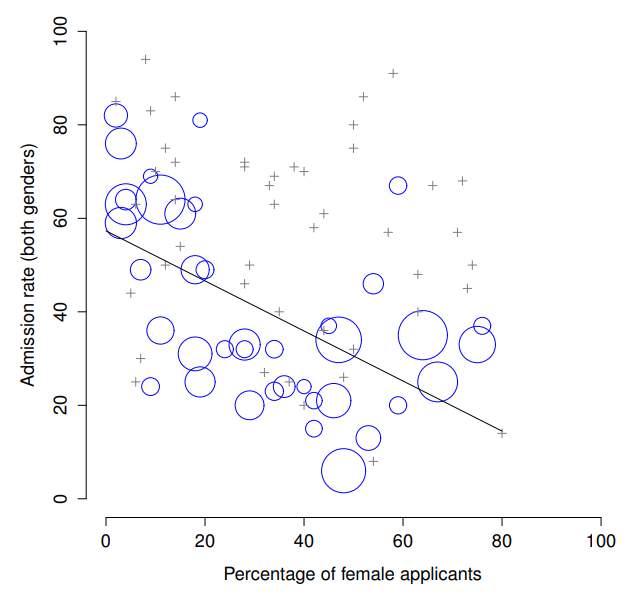
\includegraphics[width=0.9\linewidth]{images/Figure1} \caption{The Berkeley 1973 college admissions data. This figure plots the admission rate for the 85 departments that had at least one female applicant, as a function of the percentage of applicants that were female. The plot is a redrawing of Figure 1 from @Bickel1975. Circles plot departments with more than 40 applicants; the area of the circle is proportional to the total number of applicants. The crosses plot departments with fewer than 40 applicants}\label{fig:fig1-1}
\end{figure}

That was the basis for my somewhat glib remarks earlier, but that's not
exactly the whole story, is it? After all, if we're interested in this
from a more sociological and psychological perspective, we might want to
ask \emph{why} there are such strong gender differences in applications. Why
do males tend to apply to engineering more often than females, and why
is this reversed for the English department? And why is it the case that
the departments that tend to have a female-application bias tend to have
lower overall admission rates than those departments that have a
male-application bias? Might this not still reflect a gender bias, even
though every single department is itself unbiased? It might. Suppose,
hypothetically, that males preferred to apply to ``hard sciences'' and
females prefer ``humanities''. And suppose further that the reason for why
the humanities departments have low admission rates is because the
government doesn't want to fund the humanities (Ph.D.~places, for
instance, are often tied to government funded research projects). Does
that constitute a gender bias? Or just an unenlightened view of the
value of the humanities? What if someone at a high level in the
government cut the humanities funds because they felt that the
humanities are ``useless chick stuff''. That seems pretty blatantly gender
biased. None of this falls within the purview of statistics, but it
matters to the research project. If you're interested in the overall
structural effects of subtle gender biases, then you probably want to
look at both the aggregated and disaggregated data. If you're interested
in the decision making process at Berkeley itself then you're probably
only interested in the disaggregated data.That was the basis for my
somewhat glib remarks earlier, but that's not exactly the whole story,
is it? After all, if we're interested in this from a more sociological
and psychological perspective, we might want to ask why there are such
strong gender differences in applications. Why do males tend to apply to
engineering more often than females, and why is this reversed for the
English department? And why is it the case that the departments that
tend to have a female-application bias tend to have lower overall
admission rates than those departments that have a male-application
bias? Might this not still reflect a gender bias, even though every
single department is itself unbiased? It might. Suppose, hypothetically,
that males preferred to apply to ``hard sciences'' and females prefer
``humanities''. And suppose further that the reason for why the humanities
departments have low admission rates is because the government doesn't
want to fund the humanities (Ph.D.~places, for instance, are often tied
to government funded research projects). Does that constitute a gender
bias? Or just an unenlightened view of the value of the humanities? What
if someone at a high level in the government cut the humanities funds
because they felt that the humanities are ``useless chick stuff''. That
seems pretty \emph{blatantly} gender biased. None of this falls within the
purview of statistics, but it matters to the research project. If you're
interested in the overall structural effects of subtle gender biases,
then you probably want to look at \emph{both} the aggregated and
disaggregated data. If you're interested in the decision making process
at Berkeley itself then you're probably only interested in the
disaggregated data.

In short there are a lot of critical questions that you can't answer
with statistics, but the answers to those questions will have a huge
impact on how you analyse and interpret data. And this is the reason why
you should always think of statistics as a tool to help you learn about
your data. No more and no less. It's a powerful tool to that end, but
there's no substitute for careful thought.

\hypertarget{statistics-in-psychology}{%
\section{Statistics in psychology}\label{statistics-in-psychology}}

I hope that the discussion above helped explain why science in general
is so focused on statistics. But I'm guessing that you have a lot more
questions about what role statistics plays in psychology, and
specifically why psychology classes always devote so many lectures to
stats. So here's my attempt to answer a few of them\ldots{}

\textbf{Why does psychology have so much statistics?}

To be perfectly honest, there's a few different reasons, some of which
are better than others. The most important reason is that psychology is
a statistical science. What I mean by that is that the ``things'' that we
study are \emph{people}. Real, complicated, gloriously messy, infuriatingly
perverse people. The ``things'' of physics include objects like electrons,
and while there are all sorts of complexities that arise in physics,
electrons don't have minds of their own. They don't have opinions, they
don't differ from each other in weird and arbitrary ways, they don't get
bored in the middle of an experiment, and they don't get angry at the
experimenter and then deliberately try to sabotage the data set (not
that I've ever done that!). At a fundamental level psychology is harder
than physics.\footnote{Which might explain why physics is just a teensy bit further
  advanced as a science than we are.} Basically, we teach statistics to you as
psychologists because you need to be better at stats than physicists.
There's actually a saying used sometimes in physics, to the effect that
``if your experiment needs statistics, you should have done a better
experiment''. They have the luxury of being able to say that because
their objects of study are pathetically simple in comparison to the vast
mess that confronts social scientists. And it's not just psychology.
Most social sciences are desperately reliant on statistics. Not because
we're bad experimenters, but because we've picked a harder problem to
solve. We teach you stats because you really, really need it.

\textbf{Can't someone else do the statistics?}

To some extent, but not completely. It's true that you don't need to
become a fully trained statistician just to do psychology, but you do
need to reach a certain level of statistical competence. In my view,
there's three reasons that every psychological researcher ought to be
able to do basic statistics:

\begin{itemize}
\tightlist
\item
  Firstly, there's the fundamental reason: statistics is deeply
  intertwined with research design. If you want to be good at designing
  psychological studies, you need to at the very least understand the
  basics of stats.
\item
  Secondly, if you want to be good at the psychological side of the
  research, then you need to be able to understand the psychological
  literature, right? But almost every paper in the psychological
  literature reports the results of statistical analyses. So if you really
  want to understand the psychology, you need to be able to understand
  what other people did with their data. And that means understanding a
  certain amount of statistics.
\item
  Thirdly, there's a big practical problem with being dependent on
  other people to do all your statistics: statistical analysis is
  \emph{expensive}. If you ever get bored and want to look up how much the
  Australian government charges for university fees, you'll notice
  something interesting: statistics is designated as a ``national priority''
  category, and so the fees are much, much lower than for any other area
  of study. This is because there's a massive shortage of statisticians
  out there. So, from your perspective as a psychological researcher, the
  laws of supply and demand aren't exactly on your side here! As a result,
  in almost any real life situation where you want to do psychological
  research, the cruel facts will be that you don't have enough money to
  afford a statistician. So the economics of the situation mean that you
  have to be pretty self-sufficient.
\end{itemize}

Note that a lot of these reasons generalise beyond researchers. If you
want to be a practicing psychologist and stay on top of the field, it
helps to be able to read the scientific literature, which relies pretty
heavily on statistics.

\textbf{I don't care about jobs, research, or clinical work. Do I need
statistics?}

Okay, now you're just messing with me. Still, I think it should matter
to you too. Statistics should matter to you in the same way that
statistics should matter to \emph{everyone}. We live in the 21st century, and
data are \emph{everywhere}. Frankly, given the world in which we live these
days, a basic knowledge of statistics is pretty damn close to a survival
tool! Which is the topic of the next section.

\hypertarget{statistics-in-everyday-life}{%
\section{Statistics in everyday life}\label{statistics-in-everyday-life}}

\begin{quote}
\emph{``We are drowning in information,}\\
\emph{but we are starved for knowledge''}\\
- Various authors, original probably John Naisbitt
\end{quote}

When I started writing up my lecture notes I took the 20 most recent
news articles posted to the ABC news website. Of those 20 articles, it
turned out that 8 of them involved a discussion of something that I
would call a statistical topic and 6 of those made a mistake. The most
common error, if you're curious, was failing to report baseline data
(e.g., the article mentions that 5\% of people in situation X have some
characteristic Y, but doesn't say how common the characteristic is for
everyone else!). The point I'm trying to make here isn't that
journalists are bad at statistics (though they almost always are), it's
that a basic knowledge of statistics is very helpful for trying to
figure out when someone else is either making a mistake or even lying to
you. In fact, one of the biggest things that a knowledge of statistics
does to you is cause you to get angry at the newspaper or the internet
on a far more frequent basis. You can find a good example of this in the
section \protect\hyperlink{a-real-life-example}{A real life example} in the chapter on \protect\hyperlink{descriptive-statistics}{Descriptive statistics}.
In later versions of this book I'll try to include more anecdotes along
those lines.

\hypertarget{theres-more-to-research-methods-than-statistics}{%
\section{There's more to research methods than statistics}\label{theres-more-to-research-methods-than-statistics}}

So far, most of what I've talked about is statistics, and so you'd be
forgiven for thinking that statistics is all I care about in life. To be
fair, you wouldn't be far wrong, but research methodology is a broader
concept than statistics. So most research methods courses will cover a
lot of topics that relate much more to the pragmatics of research
design, and in particular the issues that you encounter when trying to
do research with humans. However, about 99\% of student fears relate to
the statistics part of the course, so I've focused on the stats in this
discussion, and hopefully I've convinced you that statistics matters,
and more importantly, that it's not to be feared. That being said, it's
pretty typical for introductory research methods classes to be very
stats-heavy. This is not (usually) because the lecturers are evil
people. Quite the contrary, in fact. Introductory classes focus a lot on
the statistics because you almost always find yourself needing
statistics before you need the other research methods training. Why?
Because almost all of your assignments in other classes will rely on
statistical training, to a much greater extent than they rely on other
methodological tools. It's not common for undergraduate assignments to
require you to design your own study from the ground up (in which case
you would need to know a lot about research design), but it \emph{is} common
for assignments to ask you to analyse and interpret data that were
collected in a study that someone else designed (in which case you need
statistics). In that sense, from the perspective of allowing you to do
well in all your other classes, the statistics is more urgent.

But note that ``urgent'' is different from ``important'' -- they both matter.
I really do want to stress that research design is just as important as
data analysis, and this book does spend a fair amount of time on it.
However, while statistics has a kind of universality, and provides a set
of core tools that are useful for most types of psychological research,
the research methods side isn't quite so universal. There are some
general principles that everyone should think about, but a lot of
research design is very idiosyncratic, and is specific to the area of
research that you want to engage in. To the extent that it's the details
that matter, those details don't usually show up in an introductory
stats and research methods class.

\begin{center}\rule{0.5\linewidth}{0.5pt}\end{center}

\hypertarget{a-brief-introduction-to-research-design}{%
\chapter{A brief introduction to research design}\label{a-brief-introduction-to-research-design}}

\begin{quote}
\emph{``To consult the statistician after an experiment is finished is often merely to ask him to conduct a post mortem examination. He can perhaps say what the experiment died of.''}\\
- Sir Ronald Fisher\footnote{Presidential Address to the First Indian Statistical Congress, 1938. Source: \href{http://en.wikiquote.org/wik\%0Ai/Ronald\%20Fisher}{http://en.wikiquote.org/wiki/Ronald Fisher}}
\end{quote}

In this chapter, we're going to start thinking about the basic ideas that go into designing a study, collecting data, checking whether your data collection works, and so on. It won't give you enough information to allow you to design studies of your own, but it will give you a lot of the basic tools that you need to assess the studies done by other people. However, since the focus of this book is much more on data analysis than on data collection, I'm only giving a very brief overview. Note that this chapter is ``special'' in two ways. Firstly, it's much more psychology specific than the later chapters. Secondly, it focuses much more heavily on the scientific problem of research methodology, and much less on the statistical problem of data analysis. Nevertheless, the two problems are related to one another, so it's traditional for stats textbooks to discuss the problem in a little detail. This chapter relies heavily on Campbell and Stanley (\protect\hyperlink{ref-Campbell1963}{1963}) and Stevens (\protect\hyperlink{ref-Stevens1946}{1946}) for the discussion of scales of measurement.

\hypertarget{introduction-to-psychological-measurement}{%
\section{Introduction to psychological measurement}\label{introduction-to-psychological-measurement}}

The first thing to understand is data collection can be thought of as a kind of \textbf{measurement}. That is, what we're trying to do here is measure something about human behaviour or the human mind. What do I mean by ``measurement''?

\hypertarget{some-thoughts-about-psychological-measurement}{%
\subsection{Some thoughts about psychological measurement}\label{some-thoughts-about-psychological-measurement}}

Measurement itself is a subtle concept, but basically it comes down to finding some way of assigning numbers, or labels, or some other kind of well-defined descriptions, to ``stuff''. So, any of the following would count as a psychological measurement:

\begin{itemize}
\tightlist
\item
  My \textbf{age} is 33 years.
\item
  I do not \textbf{like anchovies.}
\item
  My \textbf{chromosomal gender} is male.
\item
  My \textbf{self-identified gender} is female.
\end{itemize}

In the short list above, the \textbf{bolded part} is ``the thing to be measured'', and the \emph{italicised part} is ``the measurement itself''. In fact, we can expand on this a little bit, by thinking about the set of possible measurements that could have arisen in each case:

\begin{itemize}
\tightlist
\item
  My \textbf{age} (in years) could have been \emph{0, 1, 2, 3} \ldots, etc. The upper bound on what my age could possibly be is a bit fuzzy, but in practice you'd be safe in saying that the largest possible age is \emph{150}, since no human has ever lived that long.
\item
  When asked if I \textbf{like anchovies}, I might have said that \emph{I do, or I do not, or I have no opinion, or I sometimes do.}
\item
  My \textbf{chromosomal gender} is almost certainly going to be \emph{male (}\(XY\)) or \emph{female (}\(XX\)), but there are a few other possibilities. I could also have \emph{Klinfelter's syndrome} (\(XXY\)), which is more similar to male than to female. And I imagine there are other possibilities too.
\item
  My \textbf{self-identified} gender is also very likely to be male or female, but it doesn't have to agree with my chromosomal gender. I may also choose to identify with \emph{neither}, or to explicitly call myself \emph{transgender}.
\end{itemize}

As you can see, for some things (like age) it seems fairly obvious what the set of possible measurements should be, whereas for other things it gets a bit tricky. But I want to point out that even in the case of someone's age it's much more subtle than this. For instance, in the example above I assumed that it was okay to measure age in years. But if you're a developmental psychologist, that's way too crude, and so you often measure age in \emph{years and months} (if a child is 2 years and 11 months this is usually written as ``2;11''). If you're interested in newborns you might want to measure age in \emph{days since birth}, maybe even \emph{hours since birth}. In other words, the way in which you specify the allowable measurement values is important.

Looking at this a bit more closely, you might also realise that the concept of ``age'' isn't actually all that precise. In general, when we say ``age'' we implicitly mean ``the length of time since birth''. But that's not always the right way to do it. Suppose you're interested in how newborn babies control their eye movements. If you're interested in kids that young, you might also start to worry that ``birth'' is not the only meaningful point in time to care about. If Baby Alice is born 3 weeks premature and Baby Bianca is born 1 week late, would it really make sense to say that they are the ``same age'' if we encountered them ``2 hours after birth''? In one sense, yes. By social convention we use birth as our reference point for talking about age in everyday life, since it defines the amount of time the person has been operating as an independent entity in the world. But from a scientific perspective that's not the only thing we care about. When we think about the biology of human beings, it's often useful to think of ourselves as organisms that have been growing and maturing since conception, and from that perspective Alice and Bianca aren't the same age at all. So you might want to define the concept of ``age'' in two different ways: the length of time since conception and the length of time since birth. When dealing with adults it won't make much difference, but when dealing with newborns it might.

Moving beyond these issues, there's the question of methodology. What specific ``measurement method'' are you going to use to find out someone's age? As before, there are lots of different possibilities:

\begin{itemize}
\tightlist
\item
  You could just ask people ``how old are you?'' The method of self-report is fast, cheap and easy. But it only works with people old enough to understand the question, and some people lie about their age.
\item
  You could ask an authority (e.g., a parent) ``how old is your child?'' This method is fast, and when dealing with kids it's not all that hard since the parent is almost always around. It doesn't work as well if you want to know ``age since conception'', since a lot of parents can't say for sure when conception took place. For that, you might need a different authority (e.g., an obstetrician).
\item
  You could look up official records, for example birth or death certificates. This is a time consuming and frustrating endeavour, but it has its uses (e.g., if the person is now dead).
\end{itemize}

\hypertarget{operationalisation-defining-your-measurement}{%
\subsection{Operationalisation: defining your measurement}\label{operationalisation-defining-your-measurement}}

All of the ideas discussed in the previous section relate to the concept of \textbf{operationalisation}. To be a bit more precise about the idea, operationalisation is the process by which we take a meaningful but somewhat vague concept and turn it into a precise measurement. The process of operationalisation can involve several different things:

\begin{itemize}
\item
  Being precise about what you are trying to measure. For instance, does ``age'' mean ``time since birth'' or ``time since conception'' in the context of your research?
\item
  Determining what method you will use to measure it. Will you use self-report to measure age, ask a parent, or look up an official record? If you're using self-report, how will you phrase the question?
\item
  Defining the set of allowable values that the measurement can take. Note that these values don't always have to be numerical, though they often are. When measuring age the values are numerical, but we still need to think carefully about what numbers are allowed. Do we want age in years, years and months, days, or hours? For other types of measurements (e.g., gender) the values aren't numerical. But, just as before, we need to think about what values are allowed. If we're asking people to self-report their gender, what options to we allow them to choose between? Is it enough to allow only ``male'' or ``female''? Do you need an ``other'' option? Or should we not give people specific options and instead let them answer in their own words? And if you open up the set of possible values to include all verbal response, how will you interpret their answers?
\end{itemize}

Operationalisation is a tricky business, and there's no ``one, true way'' to do it. The way in which you choose to operationalise the informal concept of ``age'' or ``gender'' into a formal measurement depends on what you need to use the measurement for. Often you'll find that the community of scientists who work in your area have some fairly well-established ideas for how to go about it. In other words, operationalisation needs to be thought through on a case by case basis. Nevertheless, while there a lot of issues that are specific to each individual research project, there are some aspects to it that are pretty general.

Before moving on I want to take a moment to clear up our terminology, and in the process introduce one more term. Here are four different things that are closely related to each other:

\begin{itemize}
\tightlist
\item
  \textbf{A theoretical construct.} This is the thing that you're trying to take a measurement of, like ``age'', ``gender'' or an ``opinion''. A theoretical construct can't be directly observed, and often they're actually a bit vague.
\item
  \textbf{A measure.} The measure refers to the method or the tool that you use to make your observations. A question in a survey, a behavioural observation or a brain scan could all count as a measure.
\item
  \textbf{An operationalisation.} The term ``operationalisation'' refers to the logical connection between the measure and the theoretical construct, or to the process by which we try to derive a measure from a theoretical construct.
\item
  \textbf{A variable.} Finally, a new term. A variable is what we end up with when we apply our measure to something in the world. That is, variables are the actual ``data'' that we end up with in our data sets.
\end{itemize}

In practice, even scientists tend to blur the distinction between these things, but it's very helpful to try to understand the differences.

\hypertarget{scales-of-measurement}{%
\section{Scales of measurement}\label{scales-of-measurement}}

As the previous section indicates, the outcome of a psychological measurement is called a variable. But not all variables are of the same qualitative type and so it's useful to understand what types there are. A very useful concept for distinguishing between different types of variables is what's known as \textbf{scales of measurement}.

\hypertarget{nominal-scale}{%
\subsection{Nominal scale}\label{nominal-scale}}

A \textbf{nominal scale} variable (also referred to as a \textbf{categorical} variable) is one in which there is no particular relationship between the different possibilities. For these kinds of variables it doesn't make any sense to say that one of them is ``bigger' or''better'' than any other one, and it absolutely doesn't make any sense to average them. The classic example for this is ``eye colour''. Eyes can be blue, green or brown, amongst other possibilities, but none of them is any ``bigger'' than any other one. As a result, it would feel really weird to talk about an ``average eye colour''. Similarly, gender is nominal too: male isn't better or worse than female. Neither does it make sense to try to talk about an ``average gender''. In short, nominal scale variables are those for which the only thing you can say about the different possibilities is that they are different. That's it.

Let's take a slightly closer look at this. Suppose I was doing research on how people commute to and from work. One variable I would have to measure would be what kind of transportation people use to get to work. This ``transport type'' variable could have quite a few possible values, including: ``train'', ``bus'', ``car'', ``bicycle''. For now, let's suppose that these four are the only possibilities. Then imagine that I ask 100 people how they got to work today, with this result (Table \ref{tab:tab2-1}).

 
  \providecommand{\huxb}[2]{\arrayrulecolor[RGB]{#1}\global\arrayrulewidth=#2pt}
  \providecommand{\huxvb}[2]{\color[RGB]{#1}\vrule width #2pt}
  \providecommand{\huxtpad}[1]{\rule{0pt}{#1}}
  \providecommand{\huxbpad}[1]{\rule[-#1]{0pt}{#1}}

\begin{table}[ht]
\begin{centerbox}
\begin{threeparttable}
\setlength{\tabcolsep}{0pt}
\begin{tabular}{l l}


\hhline{>{\huxb{0, 0, 0}{0.4}}->{\huxb{0, 0, 0}{0.4}}-}
\arrayrulecolor{black}

\multicolumn{1}{!{\huxvb{0, 0, 0}{0}}c!{\huxvb{0, 0, 0}{0}}}{\cellcolor[RGB]{242, 242, 242}\huxtpad{6pt + 1em}\centering \hspace{0pt} \textbf{Transportation} \hspace{6pt}\huxbpad{6pt}} &
\multicolumn{1}{c!{\huxvb{0, 0, 0}{0}}}{\cellcolor[RGB]{242, 242, 242}\huxtpad{6pt + 1em}\centering \hspace{6pt} \textbf{Number of people} \hspace{0pt}\huxbpad{6pt}} \tabularnewline[-0.5pt]


\hhline{>{\huxb{0, 0, 0}{0.4}}->{\huxb{0, 0, 0}{0.4}}-}
\arrayrulecolor{black}

\multicolumn{1}{!{\huxvb{0, 0, 0}{0}}c!{\huxvb{0, 0, 0}{0}}}{\huxtpad{6pt + 1em}\centering \hspace{0pt} (1) Train \hspace{6pt}\huxbpad{6pt}} &
\multicolumn{1}{c!{\huxvb{0, 0, 0}{0}}}{\huxtpad{6pt + 1em}\centering \hspace{6pt} 12 \hspace{0pt}\huxbpad{6pt}} \tabularnewline[-0.5pt]


\hhline{}
\arrayrulecolor{black}

\multicolumn{1}{!{\huxvb{0, 0, 0}{0}}c!{\huxvb{0, 0, 0}{0}}}{\cellcolor[RGB]{242, 242, 242}\huxtpad{6pt + 1em}\centering \hspace{0pt} (2) Bus \hspace{6pt}\huxbpad{6pt}} &
\multicolumn{1}{c!{\huxvb{0, 0, 0}{0}}}{\cellcolor[RGB]{242, 242, 242}\huxtpad{6pt + 1em}\centering \hspace{6pt} 30 \hspace{0pt}\huxbpad{6pt}} \tabularnewline[-0.5pt]


\hhline{}
\arrayrulecolor{black}

\multicolumn{1}{!{\huxvb{0, 0, 0}{0}}c!{\huxvb{0, 0, 0}{0}}}{\huxtpad{6pt + 1em}\centering \hspace{0pt} (3) Car \hspace{6pt}\huxbpad{6pt}} &
\multicolumn{1}{c!{\huxvb{0, 0, 0}{0}}}{\huxtpad{6pt + 1em}\centering \hspace{6pt} 48 \hspace{0pt}\huxbpad{6pt}} \tabularnewline[-0.5pt]


\hhline{}
\arrayrulecolor{black}

\multicolumn{1}{!{\huxvb{0, 0, 0}{0}}c!{\huxvb{0, 0, 0}{0}}}{\cellcolor[RGB]{242, 242, 242}\huxtpad{6pt + 1em}\centering \hspace{0pt} (4) Bicycle \hspace{6pt}\huxbpad{6pt}} &
\multicolumn{1}{c!{\huxvb{0, 0, 0}{0}}}{\cellcolor[RGB]{242, 242, 242}\huxtpad{6pt + 1em}\centering \hspace{6pt} 10 \hspace{0pt}\huxbpad{6pt}} \tabularnewline[-0.5pt]


\hhline{>{\huxb{0, 0, 0}{0.4}}->{\huxb{0, 0, 0}{0.4}}-}
\arrayrulecolor{black}
\end{tabular}\captionsetup{justification=raggedright,singlelinecheck=off}
\caption{\label{tab:tab2-1} How did 100 people get to work today}
 
\end{threeparttable}\par\end{centerbox}

\end{table}
 

So, what's the average transportation type? Obviously, the answer here is that there isn't one. It's a silly question to ask. You can say that travel by car is the most popular method, and travel by train is the least popular method, but that's about all. Similarly, notice that the order in which I list the options isn't very interesting. I could have chosen to display the data like in Table \ref{tab:tab2-2}.

 
  \providecommand{\huxb}[2]{\arrayrulecolor[RGB]{#1}\global\arrayrulewidth=#2pt}
  \providecommand{\huxvb}[2]{\color[RGB]{#1}\vrule width #2pt}
  \providecommand{\huxtpad}[1]{\rule{0pt}{#1}}
  \providecommand{\huxbpad}[1]{\rule[-#1]{0pt}{#1}}

\begin{table}[ht]
\begin{centerbox}
\begin{threeparttable}
\setlength{\tabcolsep}{0pt}
\begin{tabular}{l l}


\hhline{>{\huxb{0, 0, 0}{0.4}}->{\huxb{0, 0, 0}{0.4}}-}
\arrayrulecolor{black}

\multicolumn{1}{!{\huxvb{0, 0, 0}{0}}c!{\huxvb{0, 0, 0}{0}}}{\cellcolor[RGB]{242, 242, 242}\huxtpad{6pt + 1em}\centering \hspace{0pt} \textbf{Transportation} \hspace{6pt}\huxbpad{6pt}} &
\multicolumn{1}{c!{\huxvb{0, 0, 0}{0}}}{\cellcolor[RGB]{242, 242, 242}\huxtpad{6pt + 1em}\centering \hspace{6pt} \textbf{Number of people} \hspace{0pt}\huxbpad{6pt}} \tabularnewline[-0.5pt]


\hhline{>{\huxb{0, 0, 0}{0.4}}->{\huxb{0, 0, 0}{0.4}}-}
\arrayrulecolor{black}

\multicolumn{1}{!{\huxvb{0, 0, 0}{0}}c!{\huxvb{0, 0, 0}{0}}}{\huxtpad{6pt + 1em}\centering \hspace{0pt} (3) Car \hspace{6pt}\huxbpad{6pt}} &
\multicolumn{1}{c!{\huxvb{0, 0, 0}{0}}}{\huxtpad{6pt + 1em}\centering \hspace{6pt} 48 \hspace{0pt}\huxbpad{6pt}} \tabularnewline[-0.5pt]


\hhline{}
\arrayrulecolor{black}

\multicolumn{1}{!{\huxvb{0, 0, 0}{0}}c!{\huxvb{0, 0, 0}{0}}}{\cellcolor[RGB]{242, 242, 242}\huxtpad{6pt + 1em}\centering \hspace{0pt} (1) Train \hspace{6pt}\huxbpad{6pt}} &
\multicolumn{1}{c!{\huxvb{0, 0, 0}{0}}}{\cellcolor[RGB]{242, 242, 242}\huxtpad{6pt + 1em}\centering \hspace{6pt} 12 \hspace{0pt}\huxbpad{6pt}} \tabularnewline[-0.5pt]


\hhline{}
\arrayrulecolor{black}

\multicolumn{1}{!{\huxvb{0, 0, 0}{0}}c!{\huxvb{0, 0, 0}{0}}}{\huxtpad{6pt + 1em}\centering \hspace{0pt} (4) Bicycle \hspace{6pt}\huxbpad{6pt}} &
\multicolumn{1}{c!{\huxvb{0, 0, 0}{0}}}{\huxtpad{6pt + 1em}\centering \hspace{6pt} 10 \hspace{0pt}\huxbpad{6pt}} \tabularnewline[-0.5pt]


\hhline{}
\arrayrulecolor{black}

\multicolumn{1}{!{\huxvb{0, 0, 0}{0}}c!{\huxvb{0, 0, 0}{0}}}{\cellcolor[RGB]{242, 242, 242}\huxtpad{6pt + 1em}\centering \hspace{0pt} (2) Bus \hspace{6pt}\huxbpad{6pt}} &
\multicolumn{1}{c!{\huxvb{0, 0, 0}{0}}}{\cellcolor[RGB]{242, 242, 242}\huxtpad{6pt + 1em}\centering \hspace{6pt} 30 \hspace{0pt}\huxbpad{6pt}} \tabularnewline[-0.5pt]


\hhline{>{\huxb{0, 0, 0}{0.4}}->{\huxb{0, 0, 0}{0.4}}-}
\arrayrulecolor{black}
\end{tabular}\captionsetup{justification=raggedright,singlelinecheck=off}
\caption{\label{tab:tab2-2} How did 100 people get to work today, a different view}
 
\end{threeparttable}\par\end{centerbox}

\end{table}
 

\ldots and nothing really changes.

\hypertarget{ordinal-scale}{%
\subsection{Ordinal scale}\label{ordinal-scale}}

\textbf{Ordinal scale} variables have a bit more structure than nominal scale variables, but not by a lot. An ordinal scale variable is one in which there is a natural, meaningful way to order the different possibilities, but you can't do anything else. The usual example given of an ordinal variable is ``finishing position in a race''. You \emph{can} say that the person who finished first was faster than the person who finished second, but you \emph{don't} know how much faster. As a consequence we know that 1st \(>\) 2nd, and we know that 2nd \(>\) 3rd, but the difference between 1st and 2nd might be much larger than the difference between 2nd and 3rd.

Here's a more psychologically interesting example. Suppose I'm interested in people's attitudes to climate change. I then go and ask some people to pick the statement (from four listed statements) that most closely matches their beliefs:

\begin{enumerate}
\def\labelenumi{\arabic{enumi}.}
\tightlist
\item
  Temperatures are rising because of human activity
\item
  Temperatures are rising but we don't know why
\item
  Temperatures are rising but not because of humans
\item
  Temperatures are not rising
\end{enumerate}

Notice that these four statements actually do have a natural ordering, in terms of ``the extent to which they agree with the current science''. Statement 1 is a close match, statement 2 is a reasonable match, statement 3 isn't a very good match, and statement 4 is in strong opposition to current science. So, in terms of the thing I'm interested in (the extent to which people endorse the science), I can order the items as 1 \(>\) 2 \(>\) 3 \(>\) 4. Since this ordering exists, it would be very weird to list the options like this\ldots{}

\begin{enumerate}
\def\labelenumi{\arabic{enumi}.}
\tightlist
\item
  Temperatures are rising but not because of humans
\item
  Temperatures are rising because of human activity
\item
  Temperatures are not rising
\item
  Temperatures are rising but we don't know why
\end{enumerate}

\ldots because it seems to violate the natural ``structure'' to the question.

So, let's suppose I asked 100 people these questions, and got the answers shown in Table \ref{tab:tab2-3}.

 
  \providecommand{\huxb}[2]{\arrayrulecolor[RGB]{#1}\global\arrayrulewidth=#2pt}
  \providecommand{\huxvb}[2]{\color[RGB]{#1}\vrule width #2pt}
  \providecommand{\huxtpad}[1]{\rule{0pt}{#1}}
  \providecommand{\huxbpad}[1]{\rule[-#1]{0pt}{#1}}

\begin{table}[ht]
\begin{centerbox}
\begin{threeparttable}
\setlength{\tabcolsep}{0pt}
\begin{tabular}{l l}


\hhline{>{\huxb{0, 0, 0}{0.4}}->{\huxb{0, 0, 0}{0.4}}-}
\arrayrulecolor{black}

\multicolumn{1}{!{\huxvb{0, 0, 0}{0}}c!{\huxvb{0, 0, 0}{0}}}{\cellcolor[RGB]{242, 242, 242}\huxtpad{6pt + 1em}\centering \hspace{0pt} \textbf{Response} \hspace{6pt}\huxbpad{6pt}} &
\multicolumn{1}{c!{\huxvb{0, 0, 0}{0}}}{\cellcolor[RGB]{242, 242, 242}\huxtpad{6pt + 1em}\centering \hspace{6pt} \textbf{Number} \hspace{0pt}\huxbpad{6pt}} \tabularnewline[-0.5pt]


\hhline{>{\huxb{0, 0, 0}{0.4}}->{\huxb{0, 0, 0}{0.4}}-}
\arrayrulecolor{black}

\multicolumn{1}{!{\huxvb{0, 0, 0}{0}}c!{\huxvb{0, 0, 0}{0}}}{\huxtpad{6pt + 1em}\centering \hspace{0pt} (1) Temperatures are rising because of human activity \hspace{6pt}\huxbpad{6pt}} &
\multicolumn{1}{c!{\huxvb{0, 0, 0}{0}}}{\huxtpad{6pt + 1em}\centering \hspace{6pt} 51 \hspace{0pt}\huxbpad{6pt}} \tabularnewline[-0.5pt]


\hhline{}
\arrayrulecolor{black}

\multicolumn{1}{!{\huxvb{0, 0, 0}{0}}c!{\huxvb{0, 0, 0}{0}}}{\cellcolor[RGB]{242, 242, 242}\huxtpad{6pt + 1em}\centering \hspace{0pt} (2) Temperatures are rising but we don’t know why \hspace{6pt}\huxbpad{6pt}} &
\multicolumn{1}{c!{\huxvb{0, 0, 0}{0}}}{\cellcolor[RGB]{242, 242, 242}\huxtpad{6pt + 1em}\centering \hspace{6pt} 20 \hspace{0pt}\huxbpad{6pt}} \tabularnewline[-0.5pt]


\hhline{}
\arrayrulecolor{black}

\multicolumn{1}{!{\huxvb{0, 0, 0}{0}}c!{\huxvb{0, 0, 0}{0}}}{\huxtpad{6pt + 1em}\centering \hspace{0pt} (3) Temperatures are rising but not because of humans \hspace{6pt}\huxbpad{6pt}} &
\multicolumn{1}{c!{\huxvb{0, 0, 0}{0}}}{\huxtpad{6pt + 1em}\centering \hspace{6pt} 10 \hspace{0pt}\huxbpad{6pt}} \tabularnewline[-0.5pt]


\hhline{}
\arrayrulecolor{black}

\multicolumn{1}{!{\huxvb{0, 0, 0}{0}}c!{\huxvb{0, 0, 0}{0}}}{\cellcolor[RGB]{242, 242, 242}\huxtpad{6pt + 1em}\centering \hspace{0pt} (4) Temperatures are not rising \hspace{6pt}\huxbpad{6pt}} &
\multicolumn{1}{c!{\huxvb{0, 0, 0}{0}}}{\cellcolor[RGB]{242, 242, 242}\huxtpad{6pt + 1em}\centering \hspace{6pt} 19 \hspace{0pt}\huxbpad{6pt}} \tabularnewline[-0.5pt]


\hhline{>{\huxb{0, 0, 0}{0.4}}->{\huxb{0, 0, 0}{0.4}}-}
\arrayrulecolor{black}
\end{tabular}\captionsetup{justification=raggedright,singlelinecheck=off}
\caption{\label{tab:tab2-3} Attitudes to climate change}
 
\end{threeparttable}\par\end{centerbox}

\end{table}
 

When analysing these data it seems quite reasonable to try to group (1), (2) and (3) together, and say that 81 out of 100 people were willing to at \emph{least partially} endorse the science. And it's also quite reasonable to group (2), (3) and (4) together and say that 49 out of 100 people registered \emph{at least some disagreement} with the dominant scientific view. However, it would be entirely bizarre to try to group (1), (2) and (4) together and say that 90 out of 100 people said\ldots{} what? There's nothing sensible that allows you to group those responses together at all.

That said, notice that while we \emph{can} use the natural ordering of these items to construct sensible groupings, what we can't do is average them. For instance, in my simple example here, the ``average'' response to the question is 1.97. If you can tell me what that means I'd love to know, because it seems like gibberish to me!

\hypertarget{interval-scale}{%
\subsection{Interval scale}\label{interval-scale}}

In contrast to nominal and ordinal scale variables, \textbf{interval scale} and ratio scale variables are variables for which the numerical value is genuinely meaningful. In the case of interval scale variables the \emph{differences} between the numbers are interpretable, but the variable doesn't have a ``natural'' zero value. A good example of an interval scale variable is measuring temperature in degrees celsius. For instance, if it was 15\(^{\circ}\) yesterday and 18\(^{\circ}\) today, then the 3\(^{\circ}\) difference between the two is genuinely meaningful. Moreover, that 3\(^{\circ}\) difference is \emph{exactly the same} as the 3\(^{\circ}\) difference between 7\(^{\circ}\) and 10\(^{\circ}\). In short, addition and subtraction are meaningful for interval scale variables.\footnote{Actually, I've been informed by readers with greater physics knowledge than I that temperature isn't strictly an interval scale, in the sense that the amount of energy required to heat something up by 3° depends on it's current temperature. So in the sense that physicists care about, temperature isn't actually an interval scale. But it still makes a cute example so I'm going to ignore this little inconvenient truth.}

However, notice that the 0\(^{\circ}\) does not mean ``no temperature at all''. It actually means ``the temperature at which water freezes'', which is pretty arbitrary. As a consequence it becomes pointless to try to multiply and divide temperatures. It is wrong to say that 20\(^{\circ}\) is twice as hot as 10\(^{\circ}\), just as it is weird and meaningless to try to claim that 20\(^{\circ}\) is negative two times as hot as -10\(^{\circ}\).

Again, lets look at a more psychological example. Suppose I'm interested in looking at how the attitudes of first-year university students have changed over time. Obviously, I'm going to want to record the year in which each student started. This is an interval scale variable. A student who started in 2003 did arrive 5 years before a student who started in 2008. However, it would be completely daft for me to divide 2008 by 2003 and say that the second student started ``1.0024 times later'' than the first one. That doesn't make any sense at all.

\hypertarget{ratio-scale}{%
\subsection{Ratio scale}\label{ratio-scale}}

The fourth and final type of variable to consider is a \textbf{ratio scale} variable, in which zero really means zero, and it's okay to multiply and divide. A good psychological example of a ratio scale variable is response time (RT). In a lot of tasks it's very common to record the amount of time somebody takes to solve a problem or answer a question, because it's an indicator of how difficult the task is. Suppose that Alan takes 2.3 seconds to respond to a question, whereas Ben takes 3.1 seconds. As with an interval scale variable, addition and subtraction are both meaningful here. Ben really did take 3.1 - 2.3 = 0.8 seconds longer than Alan did. However, notice that multiplication and division also make sense here too: Ben took 3.1/2.3 = 1.35 times as long as Alan did to answer the question. And the reason why you can do this is that for a ratio scale variable such as RT ``zero seconds'' really does mean ``no time at all''.

\hypertarget{continuous-versus-discrete-variables}{%
\subsection{Continuous versus discrete variables}\label{continuous-versus-discrete-variables}}

There's a second kind of distinction that you need to be aware of, regarding what types of variables you can run into. This is the distinction between continuous variables and discrete variables (Table \ref{tab:tab2-4}). The difference between these is as follows:

\begin{itemize}
\tightlist
\item
  A \textbf{continuous variable} is one in which, for any two values that you can think of, it's always logically possible to have another value in between.
\item
  A \textbf{discrete variable} is, in effect, a variable that isn't continuous. For a discrete variable it's sometimes the case that there's nothing in the middle.
\end{itemize}

 
  \providecommand{\huxb}[2]{\arrayrulecolor[RGB]{#1}\global\arrayrulewidth=#2pt}
  \providecommand{\huxvb}[2]{\color[RGB]{#1}\vrule width #2pt}
  \providecommand{\huxtpad}[1]{\rule{0pt}{#1}}
  \providecommand{\huxbpad}[1]{\rule[-#1]{0pt}{#1}}

\begin{table}[ht]
\begin{centerbox}
\begin{threeparttable}
\setlength{\tabcolsep}{0pt}
\begin{tabular}{l l l}


\hhline{>{\huxb{0, 0, 0}{0.4}}->{\huxb{0, 0, 0}{0.4}}->{\huxb{0, 0, 0}{0.4}}-}
\arrayrulecolor{black}

\multicolumn{1}{!{\huxvb{0, 0, 0}{0}}c!{\huxvb{0, 0, 0}{0}}}{\cellcolor[RGB]{242, 242, 242}\huxtpad{6pt + 1em}\centering \hspace{0pt} \textbf{} \hspace{6pt}\huxbpad{6pt}} &
\multicolumn{1}{c!{\huxvb{0, 0, 0}{0}}}{\cellcolor[RGB]{242, 242, 242}\huxtpad{6pt + 1em}\centering \hspace{6pt} \textbf{continuous} \hspace{6pt}\huxbpad{6pt}} &
\multicolumn{1}{c!{\huxvb{0, 0, 0}{0}}}{\cellcolor[RGB]{242, 242, 242}\huxtpad{6pt + 1em}\centering \hspace{6pt} \textbf{discrete} \hspace{0pt}\huxbpad{6pt}} \tabularnewline[-0.5pt]


\hhline{>{\huxb{0, 0, 0}{0.4}}->{\huxb{0, 0, 0}{0.4}}->{\huxb{0, 0, 0}{0.4}}-}
\arrayrulecolor{black}

\multicolumn{1}{!{\huxvb{0, 0, 0}{0}}c!{\huxvb{0, 0, 0}{0}}}{\huxtpad{6pt + 1em}\centering \hspace{0pt} nominal \hspace{6pt}\huxbpad{6pt}} &
\multicolumn{1}{c!{\huxvb{0, 0, 0}{0}}}{\huxtpad{6pt + 1em}\centering \hspace{6pt}  \hspace{6pt}\huxbpad{6pt}} &
\multicolumn{1}{c!{\huxvb{0, 0, 0}{0}}}{\huxtpad{6pt + 1em}\centering \hspace{6pt} ✓ \hspace{0pt}\huxbpad{6pt}} \tabularnewline[-0.5pt]


\hhline{}
\arrayrulecolor{black}

\multicolumn{1}{!{\huxvb{0, 0, 0}{0}}c!{\huxvb{0, 0, 0}{0}}}{\cellcolor[RGB]{242, 242, 242}\huxtpad{6pt + 1em}\centering \hspace{0pt} ordinal \hspace{6pt}\huxbpad{6pt}} &
\multicolumn{1}{c!{\huxvb{0, 0, 0}{0}}}{\cellcolor[RGB]{242, 242, 242}\huxtpad{6pt + 1em}\centering \hspace{6pt}  \hspace{6pt}\huxbpad{6pt}} &
\multicolumn{1}{c!{\huxvb{0, 0, 0}{0}}}{\cellcolor[RGB]{242, 242, 242}\huxtpad{6pt + 1em}\centering \hspace{6pt} ✓ \hspace{0pt}\huxbpad{6pt}} \tabularnewline[-0.5pt]


\hhline{}
\arrayrulecolor{black}

\multicolumn{1}{!{\huxvb{0, 0, 0}{0}}c!{\huxvb{0, 0, 0}{0}}}{\huxtpad{6pt + 1em}\centering \hspace{0pt} interval \hspace{6pt}\huxbpad{6pt}} &
\multicolumn{1}{c!{\huxvb{0, 0, 0}{0}}}{\huxtpad{6pt + 1em}\centering \hspace{6pt} ✓ \hspace{6pt}\huxbpad{6pt}} &
\multicolumn{1}{c!{\huxvb{0, 0, 0}{0}}}{\huxtpad{6pt + 1em}\centering \hspace{6pt} ✓ \hspace{0pt}\huxbpad{6pt}} \tabularnewline[-0.5pt]


\hhline{}
\arrayrulecolor{black}

\multicolumn{1}{!{\huxvb{0, 0, 0}{0}}c!{\huxvb{0, 0, 0}{0}}}{\cellcolor[RGB]{242, 242, 242}\huxtpad{6pt + 1em}\centering \hspace{0pt} ratio \hspace{6pt}\huxbpad{6pt}} &
\multicolumn{1}{c!{\huxvb{0, 0, 0}{0}}}{\cellcolor[RGB]{242, 242, 242}\huxtpad{6pt + 1em}\centering \hspace{6pt} ✓ \hspace{6pt}\huxbpad{6pt}} &
\multicolumn{1}{c!{\huxvb{0, 0, 0}{0}}}{\cellcolor[RGB]{242, 242, 242}\huxtpad{6pt + 1em}\centering \hspace{6pt} ✓ \hspace{0pt}\huxbpad{6pt}} \tabularnewline[-0.5pt]


\hhline{>{\huxb{0, 0, 0}{0.4}}->{\huxb{0, 0, 0}{0.4}}->{\huxb{0, 0, 0}{0.4}}-}
\arrayrulecolor{black}
\end{tabular}\captionsetup{justification=raggedright,singlelinecheck=off}
\caption{\label{tab:tab2-4} The relationship between the scales of measurement and the discrete/continuity distinction. Cells with a tick mark correspond to things that are possible}
 
\end{threeparttable}\par\end{centerbox}

\end{table}
 

These definitions probably seem a bit abstract, but they're pretty simple once you see some examples. For instance, response time is continuous. If Alan takes 3.1 seconds and Ben takes 2.3 seconds to respond to a question, then Cameron's response time will lie in between if he took 3.0 seconds. And of course it would also be possible for David to take 3.031 seconds to respond, meaning that his RT would lie in between Cameron's and Alan's. And while in practice it might be impossible to measure RT that precisely, it's certainly possible in principle. Because we can always find a new value for RT in between any two other ones we regard RT as a continuous measure.

Discrete variables occur when this rule is violated. For example, nominal scale variables are always discrete. There isn't a type of transportation that falls ``in between'' trains and bicycles, not in the strict mathematical way that 2.3 falls in between 2 and 3. So transportation type is discrete. Similarly, ordinal scale variables are always discrete. Although ``2nd place'' does fall between ``1st place'' and ``3rd place'', there's nothing that can logically fall in between ``1st place'' and ``2nd place''. Interval scale and ratio scale variables can go either way. As we saw above, response time (a ratio scale variable) is continuous. Temperature in degrees celsius (an interval scale variable) is also continuous. However, the year you went to school (an interval scale variable) is discrete. There's no year in between 2002 and 2003. The number of questions you get right on a true-or-false test (a ratio scale variable) is also discrete. Since a true-or-false question doesn't allow you to be ``partially correct'', there's nothing in between 5/10 and 6/10. Table \textbf{2.4} summarises the relationship between the scales of measurement and the discrete/continuity distinction. Cells with a tick mark correspond to things that are possible. I'm trying to hammer this point home, because (a) some textbooks get this wrong, and (b) people very often say things like ``discrete variable'' when they mean ``nominal scale variable''. It's very unfortunate.

\hypertarget{some-complexities}{%
\subsection{Some complexities}\label{some-complexities}}

Okay, I know you're going to be shocked to hear this, but the real world is much messier than this little classification scheme suggests. Very few variables in real life actually fall into these nice neat categories, so you need to be kind of careful not to treat the scales of measurement as if they were hard and fast rules. It doesn't work like that. They're guidelines, intended to help you think about the situations in which you should treat different variables differently. Nothing more.

So let's take a classic example, maybe \emph{the} classic example, of a psychological measurement tool: the \textbf{Likert scale}. The humble Likert scale is the bread and butter tool of all survey design. You yourself have filled out hundreds, maybe thousands, of them and odds are you've even used one yourself. Suppose we have a survey question that looks like this:

Which of the following best describes your opinion of the statement that ``all pirates are freaking awesome''?

and then the options presented to the participant are these:

\begin{enumerate}
\def\labelenumi{\arabic{enumi}.}
\tightlist
\item
  Strongly disagree
\item
  Disagree
\item
  Neither agree nor disagree
\item
  Agree
\item
  Strongly agree
\end{enumerate}

This set of items is an example of a 5-point Likert scale, in which people are asked to choose among one of several (in this case 5) clearly ordered possibilities, generally with a verbal descriptor given in each case. However, it's not necessary that all items are explicitly described. This is a perfectly good example of a 5-point Likert scale too:

\begin{enumerate}
\def\labelenumi{\arabic{enumi}.}
\tightlist
\item
  Strongly disagree
\item
\item
\item
\item
  Strongly agree
\end{enumerate}

Likert scales are very handy, if somewhat limited, tools. The question is what kind of variable are they? They're obviously discrete, since you can't give a response of 2.5. They're obviously not nominal scale, since the items are ordered; and they're not ratio scale either, since there's no natural zero.

But are they ordinal scale or interval scale? One argument says that we can't really prove that the difference between ``strongly agree'' and ``agree'' is of the same size as the difference between ``agree'' and ``neither agree nor disagree''. In fact, in everyday life it's pretty obvious that they're not the same at all. So this suggests that we ought to treat Likert scales as ordinal variables. On the other hand, in practice most participants do seem to take the whole ``on a scale from 1 to 5'' part fairly seriously, and they tend to act as if the differences between the five response options were fairly similar to one another. As a consequence, a lot of researchers treat Likert scale data as interval scale.\footnote{Ah, psychology\ldots{} never an easy answer to anything!} It's not interval scale, but in practice it's close enough that we usually think of it as being \textbf{quasi-interval scale}.

\hypertarget{assessing-the-reliability-of-a-measurement}{%
\section{Assessing the reliability of a measurement}\label{assessing-the-reliability-of-a-measurement}}

At this point we've thought a little bit about how to operationalise a theoretical construct and thereby create a psychological measure. And we've seen that by applying psychological measures we end up with variables, which can come in many different types. At this point, we should start discussing the obvious question: is the measurement any good? We'll do this in terms of two related ideas: \emph{reliability} and \emph{validity}. Put simply, the \textbf{reliability} of a measure tells you how precisely you are measuring something, whereas the validity of a measure tells you how accurate the measure is. In this section I'll talk about reliability; we'll talk about validity in section 2.6.

Reliability is actually a very simple concept. It refers to the repeatability or consistency of your measurement. The measurement of my weight by means of a ``bathroom scale'' is very reliable. If I step on and off the scales over and over again, it'll keep giving me the same answer. Measuring my intelligence by means of ``asking my mum'' is very unreliable. Some days she tells me I'm a bit thick, and other days she tells me I'm a complete idiot. Notice that this concept of reliability is different to the question of whether the measurements are correct (the correctness of a measurement relates to it's validity). If I'm holding a sack of potatos when I step on and off the bathroom scales the measurement will still be reliable: it will always give me the same answer. However, this highly reliable answer doesn't match up to my true weight at all, therefore it's wrong. In technical terms, this is a reliable but invalid measurement. Similarly, whilst my mum's estimate of my intelligence is a bit unreliable, she might be right. Maybe I'm just not too bright, and so while her estimate of my intelligence fluctuates pretty wildly from day to day, it's basically right. That would be an unreliable but valid measure. Of course, if my mum's estimates are too unreliable it's going to be very hard to figure out which one of her many claims about my intelligence is actually the right one. To some extent, then, a very unreliable measure tends to end up being invalid for practical purposes; so much so that many people would say that reliability is necessary (but not sufficient) to ensure validity.

Okay, now that we're clear on the distinction between reliability and validity, let's have a think about the different ways in which we might measure reliability:

\begin{itemize}
\tightlist
\item
  \textbf{Test-retest reliability}. This relates to consistency over time. If we repeat the measurement at a later date do we get a the same answer?
\item
  \textbf{Inter-rater reliability}. This relates to consistency across people. If someone else repeats the measurement (e.g., someone else rates my intelligence) will they produce the same answer?
\item
  \textbf{Parallel forms reliability}. This relates to consistency across theoretically-equivalent measurements. If I use a different set of bathroom scales to measure my weight does it give the same answer?
\item
  \textbf{Internal consistency reliability}. If a measurement is constructed from lots of different parts that perform similar functions (e.g., a personality questionnaire result is added up across several questions) do the individual parts tend to give similar answers. We'll look at this particular form of reliability later in the book, in Section 15.5.
\end{itemize}

Not all measurements need to possess all forms of reliability. For instance, educational assessment can be thought of as a form of measurement. One of the subjects that I teach, \emph{Computational Cognitive Science}, has an assessment structure that has a research component and an exam component (plus other things). The exam component is \emph{intended} to measure something different from the research component, so the assessment as a whole has low internal consistency. However, within the exam there are several questions that are intended to (approximately) measure the same things, and those tend to produce similar outcomes. So the exam on its own has a fairly high internal consistency. Which is as it should be. You should only demand reliability in those situations where you want to be measuring the same thing!

\hypertarget{the-role-of-variables-predictors-and-outcomes}{%
\section{The ``role'' of variables: predictors and outcomes}\label{the-role-of-variables-predictors-and-outcomes}}

I've got one last piece of terminology that I need to explain to you before moving away from variables. Normally, when we do some research we end up with lots of different variables. Then, when we analyse our data, we usually try to explain some of the variables in terms of some of the other variables. It's important to keep the two roles ``thing doing the explaining'' and ``thing being explained'' distinct. So let's be clear about this now. First, we might as well get used to the idea of using mathematical symbols to describe variables, since it's going to happen over and over again. Let's denote the ``to be explained'' variable \(Y\), and denote the variables ``doing the explaining'' as \(X_1 , X_2\), etc.

When we are doing an analysis we have different names for \(X\) and \(Y\), since they play different roles in the analysis. The classical names for these roles are \textbf{independent variable} (IV) and \textbf{dependent variable} (DV). The IV is the variable that you use to do the explaining (i.e., \(X\)) and the DV is the variable being explained (i.e.,\$Y \$). The logic behind these names goes like this: if there really is a relationship between \(X\) and \(Y\) then we can say that \(Y\)depends on \(X\), and if we have designed our study ``properly'' then \(X\) isn't dependent on anything else. However, I personally find those names horrible. They're hard to remember and they're highly misleading because (a) the IV is never actually ``independent of everything else'', and (b) if there's no relationship then the DV doesn't actually depend on the IV. And in fact, because I'm not the only person who thinks that IV and DV are just awful names, there are a number of alternatives that I find more appealing. The terms that I'll use in this book are \textbf{predictors} and \textbf{outcomes}. The idea here is that what you're trying to do is use \(X\) (the predictors) to make guesses about \(Y\) (the outcomes).\footnote{Annoyingly though, there's a lot of different names used out there. I won't list all of them -- there would be no point in doing that -- other than to note that ``response variable'' is sometimes used where I've used ``outcome''. Sigh. This sort of terminological confusion is very common, I'm afraid.} This is summarised in Table \ref{tab:tab2-5}.

 
  \providecommand{\huxb}[2]{\arrayrulecolor[RGB]{#1}\global\arrayrulewidth=#2pt}
  \providecommand{\huxvb}[2]{\color[RGB]{#1}\vrule width #2pt}
  \providecommand{\huxtpad}[1]{\rule{0pt}{#1}}
  \providecommand{\huxbpad}[1]{\rule[-#1]{0pt}{#1}}

\begin{table}[ht]
\begin{centerbox}
\begin{threeparttable}
\setlength{\tabcolsep}{0pt}
\begin{tabular}{l l l}


\hhline{>{\huxb{0, 0, 0}{0.4}}->{\huxb{0, 0, 0}{0.4}}->{\huxb{0, 0, 0}{0.4}}-}
\arrayrulecolor{black}

\multicolumn{1}{!{\huxvb{0, 0, 0}{0}}c!{\huxvb{0, 0, 0}{0}}}{\cellcolor[RGB]{242, 242, 242}\huxtpad{6pt + 1em}\centering \hspace{0pt} \textbf{role of the variable} \hspace{6pt}\huxbpad{6pt}} &
\multicolumn{1}{c!{\huxvb{0, 0, 0}{0}}}{\cellcolor[RGB]{242, 242, 242}\huxtpad{6pt + 1em}\centering \hspace{6pt} \textbf{classical name} \hspace{6pt}\huxbpad{6pt}} &
\multicolumn{1}{c!{\huxvb{0, 0, 0}{0}}}{\cellcolor[RGB]{242, 242, 242}\huxtpad{6pt + 1em}\centering \hspace{6pt} \textbf{modern name} \hspace{0pt}\huxbpad{6pt}} \tabularnewline[-0.5pt]


\hhline{>{\huxb{0, 0, 0}{0.4}}->{\huxb{0, 0, 0}{0.4}}->{\huxb{0, 0, 0}{0.4}}-}
\arrayrulecolor{black}

\multicolumn{1}{!{\huxvb{0, 0, 0}{0}}c!{\huxvb{0, 0, 0}{0}}}{\huxtpad{6pt + 1em}\centering \hspace{0pt} “to be explained” \hspace{6pt}\huxbpad{6pt}} &
\multicolumn{1}{c!{\huxvb{0, 0, 0}{0}}}{\huxtpad{6pt + 1em}\centering \hspace{6pt} dependent variable (DV) \hspace{6pt}\huxbpad{6pt}} &
\multicolumn{1}{c!{\huxvb{0, 0, 0}{0}}}{\huxtpad{6pt + 1em}\centering \hspace{6pt} outcome \hspace{0pt}\huxbpad{6pt}} \tabularnewline[-0.5pt]


\hhline{}
\arrayrulecolor{black}

\multicolumn{1}{!{\huxvb{0, 0, 0}{0}}c!{\huxvb{0, 0, 0}{0}}}{\cellcolor[RGB]{242, 242, 242}\huxtpad{6pt + 1em}\centering \hspace{0pt} “to do the explaining” \hspace{6pt}\huxbpad{6pt}} &
\multicolumn{1}{c!{\huxvb{0, 0, 0}{0}}}{\cellcolor[RGB]{242, 242, 242}\huxtpad{6pt + 1em}\centering \hspace{6pt} independent variable (IV) \hspace{6pt}\huxbpad{6pt}} &
\multicolumn{1}{c!{\huxvb{0, 0, 0}{0}}}{\cellcolor[RGB]{242, 242, 242}\huxtpad{6pt + 1em}\centering \hspace{6pt} predictor \hspace{0pt}\huxbpad{6pt}} \tabularnewline[-0.5pt]


\hhline{>{\huxb{0, 0, 0}{0.4}}->{\huxb{0, 0, 0}{0.4}}->{\huxb{0, 0, 0}{0.4}}-}
\arrayrulecolor{black}
\end{tabular}\captionsetup{justification=raggedright,singlelinecheck=off}
\caption{\label{tab:tab2-5} Variable distinctions}
 
\end{threeparttable}\par\end{centerbox}

\end{table}
 

\hypertarget{experimental-and-non-experimental-research}{%
\section{Experimental and non-experimental research}\label{experimental-and-non-experimental-research}}

One of the big distinctions that you should be aware of is the distinction between ``experimental research'' and ``non-experimental research''. When we make this distinction, what we're really talking about is the degree of control that the researcher exercises over the people and events in the study.

\hypertarget{experimental-research}{%
\subsection{Experimental research}\label{experimental-research}}

The key feature of \textbf{experimental research} is that the researcher controls all aspects of the study, especially what participants experience during the study. In particular, the researcher manipulates or varies the predictor variables (IVs) but allows the outcome variable (DV) to vary naturally. The idea here is to deliberately vary the predictors (IVs) to see if they have any causal effects on the outcomes. Moreover, in order to ensure that there's no possibility that something other than the predictor variables is causing the outcomes, everything else is kept constant or is in some other way ``balanced'', to ensure that they have no effect on the results. In practice, it's almost impossible to \emph{think} of everything else that might have an influence on the outcome of an experiment, much less keep it constant. The standard solution to this is \textbf{randomisation}. That is, we randomly assign people to different groups, and then give each group a different treatment (i.e., assign them different values of the predictor variables). We'll talk more about randomisation later, but for now it's enough to say that what randomisation does is minimise (but not eliminate) the possibility that there are any systematic difference between groups.

Let's consider a very simple, completely unrealistic and grossly unethical example. Suppose you wanted to find out if smoking causes lung cancer. One way to do this would be to find people who smoke and people who don't smoke and look to see if smokers have a higher rate of lung cancer. This is \emph{not} a proper experiment, since the researcher doesn't have a lot of control over who is and isn't a smoker. And this really matters. For instance, it might be that people who choose to smoke cigarettes also tend to have poor diets, or maybe they tend to work in asbestos mines, or whatever. The point here is that the groups (smokers and non-smokers) actually differ on lots of things, not just smoking. So it might be that the higher incidence of lung cancer among smokers is caused by something else, and not by smoking per se. In technical terms these other things (e.g.~diet) are called ``confounders'', and we'll talk about those in just a moment.

In the meantime, let's consider what a proper experiment might look like. Recall that our concern was that smokers and non-smokers might differ in lots of ways. The solution, as long as you have no ethics, is to control who smokes and who doesn't. Specifically, if we randomly divide young non-smokers into two groups and force half of them to become smokers, then it's very unlikely that the groups will differ in any respect other than the fact that half of them smoke. That way, if our smoking group gets cancer at a higher rate than the non-smoking group, we can feel pretty confident that (a) smoking does cause cancer and (b) we're murderers.

\hypertarget{non-experimental-research}{%
\subsection{Non-experimental research}\label{non-experimental-research}}

\textbf{Non-experimental research} is a broad term that covers ``any study in which the researcher doesn't have as much control as they do in an experiment''. Obviously, control is something that scientists like to have, but as the previous example illustrates there are lots of situations in which you can't or shouldn't try to obtain that control. Since it's grossly unethical (and almost certainly criminal) to force people to smoke in order to find out if they get cancer, this is a good example of a situation in which you really shouldn't try to obtain experimental control. But there are other reasons too. Even leaving aside the ethical issues, our ``smoking experiment'' does have a few other issues. For instance, when I suggested that we ``force'' half of the people to become smokers, I was talking about \emph{starting} with a sample of non-smokers, and then forcing them to become smokers. While this sounds like the kind of solid, evil experimental design that a mad scientist would love, it might not be a very sound way of investigating the effect in the real world. For instance, suppose that smoking only causes lung cancer when people have poor diets, and suppose also that people who normally smoke do tend to have poor diets. However, since the ``smokers'' in our experiment aren't ``natural'' smokers (i.e., we forced non-smokers to become smokers, but they didn't take on all of the other normal, real life characteristics that smokers might tend to possess) they probably have better diets. As such, in this silly example they wouldn't get lung cancer and our experiment will fail, because it violates the structure of the ``natural'' world (the technical name for this is an ``artefactual'' result).

One distinction worth making between two types of non-experimental research is the difference between \textbf{quasi-experimental research} and \textbf{case studies}. The example I discussed earlier, in which we wanted to examine incidence of lung cancer among smokers and non-smokers without trying to control who smokes and who doesn't, is a quasi-experimental design. That is, it's the same as an experiment but we don't control the predictors (IVs). We can still use statistics to analyse the results, but we have to be a lot more careful and circumspect.

The alternative approach, case studies, aims to provide a very detailed description of one or a few instances. In general, you can't use statistics to analyse the results of case studies and it's usually very hard to draw any general conclusions about ``people in general'' from a few isolated examples. However, case studies are very useful in some situations. Firstly, there are situations where you don't have any alternative. Neuropsychology has this issue a lot. Sometimes, you just can't find a lot of people with brain damage in a specific brain area, so the only thing you can do is describe those cases that you do have in as much detail and with as much care as you can. However, there's also some genuine advantages to case studies. Because you don't have as many people to study you have the ability to invest lots of time and effort trying to understand the specific factors at play in each case. This is a very valuable thing to do. As a consequence, case studies can complement the more statistically-oriented approaches that you see in experimental and quasi-experimental designs. We won't talk much about case studies in this book, but they are nevertheless very valuable tools!

\hypertarget{assessing-the-validity-of-a-study}{%
\section{Assessing the validity of a study}\label{assessing-the-validity-of-a-study}}

More than any other thing, a scientist wants their research to be ``valid''. The conceptual idea behind \textbf{validity} is very simple. Can you trust the results of your study? If not, the study is invalid. However, whilst it's easy to state, in practice it's much harder to check validity than it is to check reliability. And in all honesty, there's no precise, clearly agreed upon notion of what validity actually is. In fact, there are lots of different kinds of validity, each of which raises it's own issues. And not all forms of validity are relevant to all studies. I'm going to talk about five different types of validity:

\begin{itemize}
\tightlist
\item
  Internal validity
\item
  External validity
\item
  Construct validity
\item
  Face validity
\item
  Ecological validity
\end{itemize}

First, a quick guide as to what matters here. (1) Internal and external validity are the most important, since they tie directly to the fundamental question of whether your study really works. (2) Construct validity asks whether you're measuring what you think you are. (3) Face validity isn't terribly important except insofar as you care about ``appearances''. (4) Ecological validity is a special case of face validity that corresponds to a kind of appearance that you might care about a lot.

\hypertarget{internal-validity}{%
\subsection{Internal validity}\label{internal-validity}}

\textbf{Internal validity} refers to the extent to which you are able draw the correct conclusions about the causal relationships between variables. It's called ``internal'' because it refers to the relationships between things ``inside'' the study. Let's illustrate the concept with a simple example. Suppose you're interested in finding out whether a university education makes you write better. To do so, you get a group of first year students, ask them to write a 1000 word essay, and count the number of spelling and grammatical errors they make. Then you find some third-year students, who obviously have had more of a university education than the first-years, and repeat the exercise. And let's suppose it turns out that the third-year students produce fewer errors. And so you conclude that a university education improves writing skills. Right? Except that the big problem with this experiment is that the third-year students are older and they've had more experience with writing things. So it's hard to know for sure what the causal relationship is. Do older people write better? Or people who have had more writing experience? Or people who have had more education? Which of the above is the true cause of the superior performance of the third-years? Age? Experience? Education? You can't tell. This is an example of a failure of internal validity, because your study doesn't properly tease apart the causal relationships between the different variables.

\hypertarget{external-validity}{%
\subsection{External validity}\label{external-validity}}

\textbf{External validity} relates to the \textbf{generalisability} or \textbf{applicability} of your findings. That is, to what extent do you expect to see the same pattern of results in ``real life'' as you saw in your study. To put it a bit more precisely, any study that you do in psychology will involve a fairly specific set of questions or tasks, will occur in a specific environment, and will involve participants that are drawn from a particular subgroup (disappointingly often it is college students!). So, if it turns out that the results don't actually generalise or apply to people and situations beyond the ones that you studied, then what you've got is a lack of external validity.

The classic example of this issue is the fact that a very large proportion of studies in psychology will use undergraduate psychology students as the participants. Obviously, however, the researchers don't care \emph{only} about psychology students. They care about people in general. Given that, a study that uses only psychology students as participants always carries a risk of lacking external validity. That is, if there's something ``special'' about psychology students that makes them different to the general population in some relevant respect, then we may start worrying about a lack of external validity.

That said, it is absolutely critical to realise that a study that uses only psychology students does not necessarily have a problem with external validity. I'll talk about this again later, but it's such a common mistake that I'm going to mention it here. The external validity of a study is threatened by the choice of population if (a) the population from which you sample your participants is very narrow (e.g., psychology students), and (b) the narrow population that you sampled from is systematically different from the general population in some respect that is relevant to the \emph{psychological phenomenon that you intend to study}. The italicised part is the bit that lots of people forget. It is true that psychology undergraduates differ from the general population in lots of ways, and so a study that uses only psychology students may have problems with external validity. However, if those differences aren't very relevant to the phenomenon that you're studying, then there's nothing to worry about. To make this a bit more concrete here are two extreme examples:

\begin{itemize}
\tightlist
\item
  You want to measure ``attitudes of the general public towards psychotherapy'', but all of your participants are psychology students. This study would almost certainly have a problem with external validity.
\item
  You want to measure the effectiveness of a visual illusion, and your participants are all psychology students. This study is unlikely to have a problem with external validity
\end{itemize}

Having just spent the last couple of paragraphs focusing on the choice of participants, since that's a big issue that everyone tends to worry most about, it's worth remembering that external validity is a broader concept. The following are also examples of things that might pose a threat to external validity, depending on what kind of study you're doing:

\begin{itemize}
\tightlist
\item
  People might answer a ``psychology questionnaire'' in a manner that doesn't reflect what they would do in real life.
\item
  Your lab experiment on (say) ``human learning'' has a different structure to the learning problems people face in real life.
\end{itemize}

\hypertarget{construct-validity}{%
\subsection{Construct validity}\label{construct-validity}}

\textbf{Construct validity} is basically a question of whether you're measuring what you want to be measuring. A measurement has good construct validity if it is actually measuring the correct theoretical construct, and bad construct validity if it doesn't. To give a very simple (if ridiculous) example, suppose I'm trying to investigate the rates with which university students cheat on their exams. And the way I attempt to measure it is by asking the cheating students to stand up in the lecture theatre so that I can count them. When I do this with a class of 300 students 0 people claim to be cheaters. So I therefore conclude that the proportion of cheaters in my class is 0\%. Clearly this is a bit ridiculous. But the point here is not that this is a very deep methodological example, but rather to explain what construct validity is. The problem with my measure is that while I'm trying to measure ``the proportion of people who cheat'' what I'm actually measuring is ``the proportion of people stupid enough to own up to cheating, or bloody minded enough to pretend that they do''. Obviously, these aren't the same thing! So my study has gone wrong, because my measurement has very poor construct validity.

\hypertarget{face-validity}{%
\subsection{Face validity}\label{face-validity}}

\textbf{Face validity} simply refers to whether or not a measure ``looks like'' it's doing what it's supposed to, nothing more. If I design a test of intelligence, and people look at it and they say ``no, that test doesn't measure intelligence'', then the measure lacks face validity. It's as simple as that. Obviously, face validity isn't very important from a pure scientific perspective. After all, what we care about is whether or not the measure \emph{actually} does what it's supposed to do, not whether it \emph{looks like} it does what it's supposed to do. As a consequence, we generally don't care very much about face validity. That said, the concept of face validity serves three useful pragmatic purposes:

\begin{itemize}
\tightlist
\item
  Sometimes, an experienced scientist will have a ``hunch'' that a particular measure won't work. While these sorts of hunches have no strict evidentiary value, it's often worth paying attention to them. Because often times people have knowledge that they can't quite verbalise, so there might be something to worry about even if you can't quite say why. In other words, when someone you trust criticises the face validity of your study, it's worth taking the time to think more carefully about your design to see if you can think of reasons why it might go awry. Mind you, if you don't find any reason for concern, then you should probably not worry. After all, face validity really doesn't matter very much.
\item
  Often (very often), completely uninformed people will also have a ``hunch'' that your research is crap. And they'll criticise it on the internet or something. On close inspection you may notice that these criticisms are actually focused entirely on how the study ``looks'', but not on anything deeper. The concept of face validity is useful for gently explaining to people that they need to substantiate their arguments further.
\item
  Expanding on the last point, if the beliefs of untrained people are critical (e.g., this is often the case for applied research where you actually want to convince policy makers of something or other) then you have to care about face validity. Simply because, whether you like it or not, a lot of people will use face validity as a proxy for real validity. If you want the government to change a law on scientific psychological grounds, then it won't matter how good your studies ``really'' are. If they lack face validity you'll find that politicians ignore you. Of course, it's somewhat unfair that policy often depends more on appearance than fact, but that's how things go.
\end{itemize}

\hypertarget{ecological-validity}{%
\subsection{Ecological validity}\label{ecological-validity}}

\textbf{Ecological validity} is a different notion of validity, which is similar to external validity, but less important. The idea is that, in order to be ecologically valid, the entire set up of the study should closely approximate the real world scenario that is being investigated. In a sense, ecological validity is a kind of face validity. It relates mostly to whether the study ``looks'' right, but with a bit more rigour to it. To be ecologically valid the study has to look right in a fairly specific way. The idea behind it is the intuition that a study that is ecologically valid is more likely to be externally valid. It's no guarantee, of course. But the nice thing about ecological validity is that it's much easier to check whether a study is ecologically valid than it is to check whether a study is externally valid. A simple example would be eyewitness identification studies. Most of these studies tend to be done in a university setting, often with a fairly simple array of faces to look at, rather than a line up. The length of time between seeing the ``criminal'' and being asked to identify the suspect in the ``line up'' is usually shorter. The ``crime'' isn't real so there's no chance of the witness being scared, and there are no police officers present so there's not as much chance of feeling pressured. These things all mean that the study definitely lacks ecological validity. They might (but might not) mean that it also lacks external validity.

\hypertarget{confounds-artefacts-and-other-threats-to-validity}{%
\section{Confounds, artefacts and other threats to validity}\label{confounds-artefacts-and-other-threats-to-validity}}

If we look at the issue of validity in the most general fashion the two biggest worries that we have are \emph{confounders} and artefacts. These two terms are defined in the following way:

\begin{itemize}
\tightlist
\item
  \textbf{Confounder:} A confounder is an additional, often unmeasured variable\footnote{The reason why I say that it's unmeasured is that if you have measured it, then you can use some fancy statistical tricks to deal with the confounder. Because of the existence of these statistical solutions to the problem of confounders, we often refer to a confounder that we have measured and dealt with as a covariate. Dealing with covariates is a more advanced topic, but I thought I'd mention it in passing since it's kind of comforting to at least know that this stuff exists.} that turns out to be related to both the predictors and the outcome. The existence of confounders threatens the internal validity of the study because you can't tell whether the predictor causes the outcome, or if the confounding variable causes it.
\item
  \textbf{Artefact:} A result is said to be ``artefactual'' if it only holds in the special situation that you happened to test in your study. The possibility that your result is an artefact describes a threat to your external validity, because it raises the possibility that you can't generalise or apply your results to the actual population that you care about.
\end{itemize}

As a general rule confounders are a bigger concern for non-experimental studies, precisely because they're not proper experiments. By definition, you're leaving lots of things uncontrolled, so there's a lot of scope for confounders being present in your study. Experimental research tends to be much less vulnerable to confounders. The more control you have over what happens during the study, the more you can prevent confounders from affecting the results. With random allocation, for example, confounders are distributed randomly, and evenly, between different groups.

However, there are always swings and roundabouts and when we start thinking about artefacts rather than confounders the shoe is very firmly on the other foot. For the most part, artefactual results tend to be a concern for experimental studies than for non-experimental studies. To see this, it helps to realise that the reason that a lot of studies are non-experimental is precisely because what the researcher is trying to do is examine human behaviour in a more naturalistic context. By working in a more real-world context you lose experimental control (making yourself vulnerable to confounders), but because you tend to be studying human psychology ``in the wild'' you reduce the chances of getting an artefactual result. Or, to put it another way, when you take psychology out of the wild and bring it into the lab (which we usually have to do to gain our experimental control), you always run the risk of accidentally studying something different to what you wanted to study.

Be warned though. The above is a rough guide only. It's absolutely possible to have confounders in an experiment, and to get artefactual results with non-experimental studies. This can happen for all sorts of reasons, not least of which is experimenter or researcher error. In practice, it's really hard to think everything through ahead of time and even very good researchers make mistakes.

Although there's a sense in which almost any threat to validity can be characterised as a confounder or an artefact, they're pretty vague concepts. So let's have a look at some of the most common examples.

\hypertarget{history-effects}{%
\subsection{History effects}\label{history-effects}}

\textbf{History effects} refer to the possibility that specific events may occur during the study that might influence the outcome measure. For instance, something might happen in between a pretest and a post-test. Or in-between testing participant 23 and participant 24. Alternatively, it might be that you're looking at a paper from an older study that was perfectly valid for its time, but the world has changed enough since then that the conclusions are no longer trustworthy. Examples of things that would count as history effects are:

\begin{itemize}
\item
  You're interested in how people think about risk and uncertainty. You started your data collection in December 2010. But finding participants and collecting data takes time, so you're still finding new people in February 2011. Unfortunately for you (and even more unfortunately for others), the Queensland floods occurred in January 2011 causing billions of dollars of damage and killing many people. Not surprisingly, the people tested in February 2011 express quite different beliefs about handling risk than the people tested in December 2010. Which (if any) of these reflects the ``true'' beliefs of participants? I think the answer is probably both. The Queensland floods genuinely changed the beliefs of the Australian public, though possibly only temporarily. The key thing here is that the ``history'' of the people tested in February is quite different to people tested in December.
\item
  You're testing the psychological effects of a new anti-anxiety drug. So what you do is measure anxiety before administering the drug (e.g., by self-report, and taking physiological measures). Then you administer the drug, and afterwards you take the same measures. In the middle however, because your lab is in Los Angeles, there's an earthquake which increases the anxiety of the participants.
\end{itemize}

\hypertarget{maturation-effects}{%
\subsection{Maturation effects}\label{maturation-effects}}

As with history effects, \textbf{maturational effects} are fundamentally about change over time. However, maturation effects aren't in response to specific events. Rather, they relate to how people change on their own over time. We get older, we get tired, we get bored, etc. Some examples of maturation effects are:

\begin{itemize}
\tightlist
\item
  When doing developmental psychology research you need to be aware that children grow up quite rapidly. So, suppose that you want to find out whether some educational trick helps with vocabulary size among 3 year olds. One thing that you need to be aware of is that the vocabulary size of children that age is growing at an incredible rate (multiple words per day) all on its own. If you design your study without taking this maturational effect into account, then you won't be able to tell if your educational trick works.
\item
  When running a very long experiment in the lab (say, something that goes for 3 hours) it's very likely that people will begin to get bored and tired, and that this maturational effect will cause performance to decline regardless of anything else going on in the experiment
\end{itemize}

\hypertarget{repeated-testing-effects}{%
\subsection{Repeated testing effects}\label{repeated-testing-effects}}

An important type of history effect is the effect of \textbf{repeated testing}. Suppose I want to take two measurements of some psychological construct (e.g., anxiety). One thing I might be worried about is if the first measurement has an effect on the second measurement. In other words, this is a history effect in which the ``event'' that influences the second measurement is the first measurement itself! This is not at all uncommon. Examples of this include:

\begin{itemize}
\tightlist
\item
  Learning and practice: e.g., ``intelligence'' at time 2 might appear to go up relative to time 1 because participants learned the general rules of how to solve ``intelligence-test-style'' questions during the first testing session.
\item
  Familiarity with the testing situation: e.g., if people are nervous at time 1, this might make performance go down. But after sitting through the first testing situation they might calm down a lot precisely because they've seen what the testing looks like.
\item
  Auxiliary changes caused by testing: e.g., if a questionnaire assessing mood is boring then mood rating at measurement time 2 is more likely to be ``bored'' precisely because of the boring measurement made at time 1.
\end{itemize}

\hypertarget{selection-bias}{%
\subsection{Selection bias}\label{selection-bias}}

\textbf{Selection bias} is a pretty broad term. Suppose that you're running an experiment with two groups of participants where each group gets a different ``treatment'', and you want to see if the different treatments lead to different outcomes. However, suppose that, despite your best efforts, you've ended up with a gender imbalance across groups (say, group A has 80\% females and group B has 50\% females). It might sound like this could never happen but, trust me, it can. This is an example of a selection bias, in which the people ``selected into'' the two groups have different characteristics. If any of those characteristics turns out to be relevant (say, your treatment works better on females than males) then you're in a lot of trouble.

\hypertarget{differential-attrition}{%
\subsection{Differential attrition}\label{differential-attrition}}

When thinking about the effects of attrition, it is sometimes helpful to distinguish between two different types. The first is \textbf{homogeneous attrition}, in which the attrition effect is the same for all groups, treatments or conditions. In the example I gave above, the attrition would be homogeneous if (and only if) the easily bored participants are dropping out of all of the conditions in my experiment at about the same rate. In general, the main effect of homogeneous attrition is likely to be that it makes your sample unrepresentative. As such, the biggest worry that you'll have is that the generalisability of the results decreases. In other words, you lose external validity.

The second type of attrition is \textbf{heterogeneous attrition}, in which the attrition effect is different for different groups. More often called \textbf{differential attrition}, this is a kind of selection bias that is caused by the study itself. Suppose that, for the first time ever in the history of psychology, I manage to find the perfectly balanced and representative sample of people. I start running ``Dani's incredibly long and tedious experiment'' on my perfect sample but then, because my study is incredibly long and tedious, lots of people start dropping out. I can't stop this. Participants absolutely have the right to stop doing any experiment, any time, for whatever reason they feel like, and as researchers we are morally (and professionally) obliged to remind people that they do have this right. So, suppose that ``Dani's incredibly long and tedious experiment'' has a very high drop out rate. What do you suppose the odds are that this drop out is random? Answer: zero. Almost certainly the people who remain are more conscientious, more tolerant of boredom, etc., than those that leave. To the extent that (say) conscientiousness is relevant to the psychological phenomenon that I care about, this attrition can decrease the validity of my results.

Here's another example. Suppose I design my experiment with two conditions. In the ``treatment'' condition, the experimenter insults the participant and then gives them a questionnaire designed to measure obedience. In the ``control'' condition, the experimenter engages in a bit of pointless chitchat and then gives them the questionnaire. Leaving aside the questionable scientific merits and dubious ethics of such a study, let's have a think about what might go wrong here. As a general rule, when someone insults me to my face I tend to get much less co-operative. So, there's a pretty good chance that a lot more people are going to drop out of the treatment condition than the control condition. And this drop out isn't going to be random. The people most likely to drop out would probably be the people who don't care all that much about the importance of obediently sitting through the experiment. Since the most bloody minded and disobedient people all left the treatment group but not the control group, we've introduced a confound: the people who actually took the questionnaire in the treatment group were already more likely to be dutiful and obedient than the people in the control group. In short, in this study insulting people doesn't make them more obedient. It makes the more disobedient people leave the experiment! The internal validity of this experiment is completely shot.

\hypertarget{non-response-bias}{%
\subsection{Non-response bias}\label{non-response-bias}}

\textbf{Non-response bias} is closely related to selection bias and to differential attrition. The simplest version of the problem goes like this. You mail out a survey to 1000 people but only 300 of them reply. The 300 people who replied are almost certainly not a random subsample. People who respond to surveys are systematically different to people who don't. This introduces a problem when trying to generalise from those 300 people who replied to the population at large, since you now have a very non-random sample. The issue of non-response bias is more general than this, though. Among the (say) 300 people that did respond to the survey, you might find that not everyone answers every question. If (say) 80 people chose not to answer one of your questions, does this introduce problems? As always, the answer is maybe. If the question that wasn't answered was on the last page of the questionnaire, and those 80 surveys were returned with the last page missing, there's a good chance that the missing data isn't a big deal; probably the pages just fell off. However, if the question that 80 people didn't answer was the most confrontational or invasive personal question in the questionnaire, then almost certainly you've got a problem. In essence, what you're dealing with here is what's called the problem of \textbf{missing data}. If the data that is missing was ``lost'' randomly, then it's not a big problem. If it's missing systematically, then it can be a big problem.

\hypertarget{regression-to-the-mean}{%
\subsection{Regression to the mean}\label{regression-to-the-mean}}

\textbf{Regression to the mean} refers to any situation where you select data based on an extreme value on some measure. Because the variable has natural variation it almost certainly means that when you take a subsequent measurement the later measurement will be less extreme than the first one, purely by chance.

Here's an example. Suppose I'm interested in whether a psychology education has an adverse effect on very smart kids. To do this, I find the 20 psychology I students with the best high school grades and look at how well they're doing at university. It turns out that they're doing a lot better than average, but they're not topping the class at university even though they did top their classes at high school. What's going on? The natural first thought is that this must mean that the psychology classes must be having an adverse effect on those students. However, while that might very well be the explanation, it's more likely that what you're seeing is an example of ``regression to the mean''. To see how it works, let's take a moment to think about what is required to get the best mark in a class, regardless of whether that class be at high school or at university. When you've got a big class there are going to be lots of very smart people enrolled. To get the best mark you have to be very smart, work very hard, and be a bit lucky. The exam has to ask just the right questions for your idiosyncratic skills, and you have to avoid making any dumb mistakes (we all do that sometimes) when answering them. And that's the thing, whilst intelligence and hard work are transferable from one class to the next, luck isn't. The people who got lucky in high school won't be the same as the people who get lucky at university. That's the very definition of ``luck''. The consequence of this is that when you select people at the very extreme values of one measurement (the top 20 students), you're selecting for hard work, skill and luck. But because the luck doesn't transfer to the second measurement (only the skill and work), these people will all be expected to drop a little bit when you measure them a second time (at university). So their scores fall back a little bit, back towards everyone else. This is regression to the mean.

Regression to the mean is surprisingly common. For instance, if two very tall people have kids their children will tend to be taller than average but not as tall as the parents. The reverse happens with very short parents. Two very short parents will tend to have short children, but nevertheless those kids will tend to be taller than the parents. It can also be extremely subtle. For instance, there have been studies done that suggested that people learn better from negative feedback than from positive feedback. However, the way that people tried to show this was to give people positive reinforcement whenever they did good, and negative reinforcement when they did bad. And what you see is that after the positive reinforcement people tended to do worse, but after the negative reinforcement they tended to do better. But notice that there's a selection bias here! When people do very well, you're selecting for ``high'' values, and so you should expect, because of regression to the mean, that performance on the next trial should be worse regardless of whether reinforcement is given. Similarly, after a bad trial, people will tend to improve all on their own. The apparent superiority of negative feedback is an artefact caused by regression to the mean (see Kahneman and Tversky (\protect\hyperlink{ref-Kahneman1973}{1973}), for discussion).

\hypertarget{experimenter-bias}{%
\subsection{Experimenter bias}\label{experimenter-bias}}

\textbf{Experimenter bias} can come in multiple forms. The basic idea is that the experimenter, despite the best of intentions, can accidentally end up influencing the results of the experiment by subtly communicating the ``right answer'' or the ``desired behaviour'' to the participants. Typically, this occurs because the experimenter has special knowledge that the participant does not, for example the right answer to the questions being asked or knowledge of the expected pattern of performance for the condition that the participant is in. The classic example of this happening is the case study of ``Clever Hans'', which dates back to 1907 (\protect\hyperlink{ref-Pfungst1911}{Pfungst 1911}). Clever Hans was a horse that apparently was able to read and count and perform other human like feats of intelligence. After Clever Hans became famous, psychologists started examining his behaviour more closely. It turned out that, not surprisingly, Hans didn't know how to do maths. Rather, Hans was responding to the human observers around him, because the humans did know how to count and the horse had learned to change its behaviour when people changed theirs.

The general solution to the problem of experimenter bias is to engage in double blind studies, where neither the experimenter nor the participant knows which condition the participant is in or knows what the desired behaviour is. This provides a very good solution to the problem, but it's important to recognise that it's not quite ideal, and hard to pull off perfectly. For instance, the obvious way that I could try to construct a double blind study is to have one of my Ph.D.~students (one who doesn't know anything about the experiment) run the study. That feels like it should be enough. The only person (me) who knows all the details (e.g., correct answers to the questions, assignments of participants to conditions) has no interaction with the participants, and the person who does all the talking to people (the Ph.D.~student) doesn't know anything. Except for the reality that the last part is very unlikely to be true. In order for the Ph.D.~student to run the study effectively they need to have been briefed by me, the researcher. And, as it happens, the Ph.D.~student also knows me and knows a bit about my general beliefs about people and psychology (e.g., I tend to think humans are much smarter than psychologists give them credit for). As a result of all this, it's almost impossible for the experimenter to avoid knowing a little bit about what expectations I have. And even a little bit of knowledge can have an effect. Suppose the experimenter accidentally conveys the fact that the participants are expected to do well in this task. Well, there's a thing called the ``Pygmalion effect'', where if you expect great things of people they'll tend to rise to the occasion. But if you expect them to fail then they'll do that too. In other words, the expectations become a self-fulfilling prophesy.

\hypertarget{demand-effects-and-reactivity}{%
\subsection{Demand effects and reactivity}\label{demand-effects-and-reactivity}}

When talking about experimenter bias, the worry is that the experimenter's knowledge or desires for the experiment are communicated to the participants, and that these can change people's behaviour (\protect\hyperlink{ref-Rosenthal1966}{Rosenthal 1966}). However, even if you manage to stop this from happening, it's almost impossible to stop people from knowing that they're part of a psychological study. And the mere fact of knowing that someone is watching or studying you can have a pretty big effect on behaviour. This is generally referred to as \textbf{reactivity} or \textbf{demand effects}. The basic idea is captured by the Hawthorne effect: people alter their performance because of the attention that the study focuses on them. The effect takes its name from a study that took place in the ``Hawthorne Works'' factory outside of Chicago (see Adair (\protect\hyperlink{ref-Adair1984}{1984})). This study, from the 1920s, looked at the effects of factory lighting on worker productivity. But, importantly, change in worker behaviour occurred because the workers knew they were being studied, rather than any effect of factory lighting.

To get a bit more specific about some of the ways in which the mere fact of being in a study can change how people behave, it helps to think like a social psychologist and look at some of the roles that people might adopt during an experiment but might not adopt if the corresponding events were occurring in the real world:

\begin{itemize}
\tightlist
\item
  The \emph{good participant} tries to be too helpful to the researcher. He or she seeks to figure out the experimenter's hypotheses and confirm them.
\item
  The \emph{negative participant} does the exact opposite of the good participant. He or she seeks to break or destroy the study or the hypothesis in some way.
\item
  The \emph{faithful participant} is unnaturally obedient. He or she seeks to follow instructions perfectly, regardless of what might have happened in a more realistic setting.
\item
  The \emph{apprehensive participant} gets nervous about being tested or studied, so much so that his or her behaviour becomes highly unnatural, or overly socially desirable.
\end{itemize}

\hypertarget{placebo-effects}{%
\subsection{Placebo effects}\label{placebo-effects}}

The \textbf{placebo effect} is a specific type of demand effect that we worry a lot about. It refers to the situation where the mere fact of being treated causes an improvement in outcomes. The classic example comes from clinical trials. If you give people a completely chemically inert drug and tell them that it's a cure for a disease, they will tend to get better faster than people who aren't treated at all. In other words, it is people's belief that they are being treated that causes the improved outcomes, not the drug.

However, the current consensus in medicine is that true placebo effects are quite rare and most of what was previously considered placebo effect is in fact some combination of natural healing (some people just get better on their own), regression to the mean and other quirks of study design. Of interest to psychology is that the strongest evidence for at least some placebo effect is in self-reported outcomes, most notably in treatment of pain (\protect\hyperlink{ref-hrobjartsson2010}{Hróbjartsson and Gøtzsche 2010}).

\hypertarget{situation-measurement-and-sub-population-effects}{%
\subsection{Situation, measurement and sub-population effects}\label{situation-measurement-and-sub-population-effects}}

In some respects, these terms are a catch-all term for ``all other threats to external validity''. They refer to the fact that the choice of sub-population from which you draw your participants, the location, timing and manner in which you run your study (including who collects the data) and the tools that you use to make your measurements might all be influencing the results. Specifically, the worry is that these things might be influencing the results in such a way that the results won't generalise to a wider array of people, places and measures.

\hypertarget{fraud-deception-and-self-deception}{%
\subsection{Fraud, deception and self-deception}\label{fraud-deception-and-self-deception}}

\begin{quote}
\emph{It is difficult to get a man to understand something, when his salary depends on his not understanding it.}\\
- Upton Sinclair
\end{quote}

There's one final thing I feel I should mention. While reading what the textbooks often have to say about assessing the validity of a study I couldn't help but notice that they seem to make the assumption that the researcher is honest. I find this hilarious. While the vast majority of scientists are honest, in my experience at least, some are not.\footnote{Some people might argue that if you're not honest then you're not a real scientist. Which does have some truth to it I guess, but that's disingenuous (look up the ``No true Scotsman'' fallacy). The fact is that there are lots of people who are employed ostensibly as scientists, and whose work has all of the trappings of science, but who are outright fraudulent. Pretending that they don't exist by saying that they're not scientists is just muddled thinking.} Not only that, as I mentioned earlier, scientists are not immune to belief bias. It's easy for a researcher to end up deceiving themselves into believing the wrong thing, and this can lead them to conduct subtly flawed research and then hide those flaws when they write it up. So you need to consider not only the (probably unlikely) possibility of outright fraud, but also the (probably quite common) possibility that the research is unintentionally ``slanted''. I opened a few standard textbooks and didn't find much of a discussion of this problem, so here's my own attempt to list a few ways in which these issues can arise:

\begin{itemize}
\tightlist
\item
  \textbf{Data fabrication}. Sometimes, people just make up the data. This is occasionally done with ``good'' intentions. For instance, the researcher believes that the fabricated data do reflect the truth, and may actually reflect ``slightly cleaned up'' versions of actual data. On other occasions, the fraud is deliberate and malicious. Some high-profile examples where data fabrication has been alleged or shown include Cyril Burt (a psychologist who is thought to have fabricated some of his data), Andrew Wakefield (who has been accused of fabricating his data connecting the MMR vaccine to autism) and Hwang Woo-suk (who falsified a lot of his data on stem cell research).
\item
  \textbf{Hoaxes}. Hoaxes share a lot of similarities with data fabrication, but they differ in the intended purpose. A hoax is often a joke, and many of them are intended to be (eventually) discovered. Often, the point of a hoax is to discredit someone or some field. There's quite a few well known scientific hoaxes that have occurred over the years (e.g., Piltdown man) and some were deliberate attempts to discredit particular fields of research (e.g., the Sokal affair).
\item
  \textbf{Data misrepresentation}. While fraud gets most of the headlines, it's much more common in my experience to see data being misrepresented. When I say this I'm not referring to newspapers getting it wrong (which they do, almost always). I'm referring to the fact that often the data don't actually say what the researchers think they say. My guess is that, almost always, this isn't the result of deliberate dishonesty but instead is due to a lack of sophistication in the data analyses. For instance, think back to the example of Simpson's paradox that I discussed in the beginning of this book. It's very common to see people present ``aggregated'' data of some kind and sometimes, when you dig deeper and find the raw data yourself you find that the aggregated data tell a different story to the disaggregated data. Alternatively, you might find that some aspect of the data is being hidden, because it tells an inconvenient story (e.g., the researcher might choose not to refer to a particular variable). There's a lot of variants on this, many of which are very hard to detect.
\item
  \textbf{Study ``misdesign''}. Okay, this one is subtle. Basically, the issue here is that a researcher designs a study that has built-in flaws and those flaws are never reported in the paper. The data that are reported are completely real and are correctly analysed, but they are produced by a study that is actually quite wrongly put together. The researcher really wants to find a particular effect and so the study is set up in such a way as to make it ``easy'' to (artefactually) observe that effect. One sneaky way to do this, in case you're feeling like dabbling in a bit of fraud yourself, is to design an experiment in which it's obvious to the participants what they're ``supposed'' to be doing, and then let reactivity work its magic for you. If you want you can add all the trappings of double blind experimentation but it won't make a difference since the study materials themselves are subtly telling people what you want them to do. When you write up the results the fraud won't be obvious to the reader. What's obvious to the participant when they're in the experimental context isn't always obvious to the person reading the paper. Of course, the way I've described this makes it sound like it's always fraud. Probably there are cases where this is done deliberately, but in my experience the bigger concern has been with unintentional misdesign. The researcher believes and so the study just happens to end up with a built in flaw, and that flaw then magically erases itself when the study is written up for publication.
\item
  \textbf{Data mining \& post hoc hypothesising}. Another way in which the authors of a study can more or less misrepresent the data is by engaging in what's referred to as ``data mining'' (see Gelman and Loken 2014, for a broader discussion of this as part of the ``garden of forking paths'' in statistical analysis). As we'll discuss later, if you keep trying to analyse your data in lots of different ways, you'll eventually find something that ``looks'' like a real effect but isn't. This is referred to as ``data mining''. It used to be quite rare because data analysis used to take weeks, but now that everyone has very powerful statistical software on their computers it's becoming very common. Data mining per se isn't ``wrong'', but the more that you do it the bigger the risk you're taking. The thing that is wrong, and I suspect is very common, is unacknowledged data mining. That is, the researcher runs every possible analysis known to humanity, finds the one that works, and then pretends that this was the only analysis that they ever conducted. Worse yet, they often ``invent'' a hypothesis after looking at the data to cover up the data mining. To be clear. It's not wrong to change your beliefs after looking at the data, and to reanalyse your data using your new ``post hoc'' hypotheses. What is wrong (and I suspect common) is failing to acknowledge that you've done. If you acknowledge that you did it then other researchers are able to take your behaviour into account. If you don't, then they can't. And that makes your behaviour deceptive. Bad!
\item
  \textbf{Publication bias \& self-censoring}. Finally, a pervasive bias is ``non-reporting'' of negative results. This is almost impossible to prevent. Journals don't publish every article that is submitted to them. They prefer to publish articles that find ``something''. So, if 20 people run an experiment looking at whether reading Finnegans Wake causes insanity in humans, and 19 of them find that it doesn't, which one do you think is going to get published? Obviously, it's the one study that did find that Finnegans Wake causes insanity.\footnote{Clearly, the real effect is that only insane people would even try to read \emph{Finnegans Wake}} This is an example of a publication bias. Since no-one ever published the 19 studies that didn't find an effect, a naive reader would never know that they existed. Worse yet, most researchers ``internalise'' this bias and end up self-censoring their research. Knowing that negative results aren't going to be accepted for publication, they never even try to report them. As a friend of mine says ``for every experiment that you get published, you also have 10 failures''. And she's right. The catch is, while some (maybe most) of those studies are failures for boring reasons (e.g.~you stuffed something up) others might be genuine ``null'' results that you ought to acknowledge when you write up the ``good'' experiment. And telling which is which is often hard to do. A good place to start is a paper by Ioannidis (\protect\hyperlink{ref-Ioannidis2005}{2005}) with the depressing title ``Why most published research findings are false''. I'd also suggest taking a look at work by Kühberger, Fritz, and Scherndl (\protect\hyperlink{ref-Kuhberger2014}{2014}) presenting statistical evidence that this actually happens in psychology.
\end{itemize}

There's probably a lot more issues like this to think about, but that'll do to start with. What I really want to point out is the blindingly obvious truth that real world science is conducted by actual humans, and only the most gullible of people automatically assumes that everyone else is honest and impartial. Actual scientists aren't usually that naive, but for some reason the world likes to pretend that we are, and the textbooks we usually write seem to reinforce that stereotype.

\hypertarget{summary}{%
\section{Summary}\label{summary}}

This chapter isn't really meant to provide a comprehensive discussion of psychological research methods. It would require another volume just as long as this one to do justice to the topic. However, in real life statistics and study design are so tightly intertwined that it's very handy to discuss some of the key topics. In this chapter, I've briefly discussed the following topics:

\begin{itemize}
\tightlist
\item
  \protect\hyperlink{introduction-to-psychological-measurement}{Introduction to psychological measurement}. What does it mean to operationalise a theoretical construct? What does it mean to have variables and take measurements?
\item
  \protect\hyperlink{scales-of-measurement}{Scales of measurement} and types of variables. Remember that there are two different distinctions here. There's the difference between discrete and continuous data, and there's the difference between the four different scale types (nominal, ordinal, interval and ratio).
\item
  \protect\hyperlink{assessing-the-reliability-of-a-measurement}{Assessing the reliability of a measurement}. If I measure the ``same'' thing twice, should I expect to see the same result? Only if my measure is reliable. But what does it mean to talk about doing the ``same'' thing? Well, that's why we have different types of reliability. Make sure you remember what they are.
\item
  \protect\hyperlink{the-role-of-variables-predictors-and-outcomes}{The ``role'' of variables: predictors and outcomes}. What roles do variables play in an analysis? Can you remember the difference between predictors and outcomes? Dependent and independent variables? Etc.
\item
  \protect\hyperlink{experimental-and-non-experimental-research}{Experimental and non-experimental research} designs. What makes an experiment an experiment? Is it a nice white lab coat, or does it have something to do with researcher control over variables?
\item
  \protect\hyperlink{assessing-the-validity-of-a-study}{Assessing the validity of a study}. Does your study measure what you want it to? How might things go wrong? And is it my imagination, or was that a very long list of possible ways in which things can go wrong?
\end{itemize}

All this should make clear to you that study design is a critical part of research methodology. I built this chapter from the classic little book by Campbell and Stanley (\protect\hyperlink{ref-Campbell1963}{1963}), but there are of course a large number of textbooks out there on research design. Spend a few minutes with your favourite search engine and you'll find dozens.

\begin{center}\rule{0.5\linewidth}{0.5pt}\end{center}

\hypertarget{getting-started-with-jamovi}{%
\chapter{Getting started with jamovi}\label{getting-started-with-jamovi}}

\begin{quote}
\emph{Robots are nice to work with.}\\
- Roger Zelazny\footnote{Source: Dismal Light (1968).}
\end{quote}

In this chapter I'll discuss how to get started in jamovi. I'll briefly
talk about how to download and install jamovi, but most of the chapter
will be focused on getting you started with finding your way around the
jamovi GUI. Our goal in this chapter is not to learn any statistical
concepts: we're just trying to learn the basics of how jamovi works and
get comfortable interacting with the system. To do this we'll spend a
bit of time looking at datasets and variables. In doing so, you'll get a
bit of a feel for what it's like to work in jamovi.

However, before going into any of the specifics, it's worth talking a
little about why you might want to use jamovi at all. Given that you're
reading this you've probably got your own reasons. However, if those
reasons are ``because that's what my stats class uses'', it might be worth
explaining a little why your lecturer has chosen to use jamovi for the
class. Of course, I don't really know why \emph{other} people choose jamovi
so I'm really talking about why I use it.

\begin{itemize}
\tightlist
\item
  It's sort of obvious but worth saying anyway: doing your statistics
  on a computer is faster, easier and more powerful than doing
  statistics by hand. Computers excel at mindless repetitive tasks,
  and a lot of statistical calculations are both mindless and
  repetitive. For most people the only reason to ever do statistical
  calculations with pencil and paper is for learning purposes. In my
  class I do occasionally suggest doing some calculations that way,
  but the only real value to it is pedagogical. It does help you to
  get a ``feel'' for statistics to do some calculations yourself, so
  it's worth doing it once. But only once!
\item
  Doing statistics in a conventional spreadsheet (e.g., Microsoft
  Excel) is generally a bad idea in the long run. Although many people
  likely feel more familiar with them, spreadsheets are very limited
  in terms of what analyses they allow you do. If you get into the
  habit of trying to do your real life data analysis using
  spreadsheets then you've dug yourself into a very deep hole.
\item
  ``student versions'' (crippled versions of the real thing) very
  cheaply, and then they they sell full powered ``educational versions''
  at a price that makes me wince. They will also sell commercial
  licences with a staggeringly high price tag. The business model here
  is to suck you in during your student days and then leave you
  dependent on their tools when you go out into the real world. It's
  hard to blame them for trying, but personally I'm not in favour of
  shelling out thousands of dollars if I can avoid it. And you can
  avoid it. If you make use of packages like jamovi that are open
  source and free you never get trapped having to pay exorbitant
  licensing fees.
\item
  Something that you might not appreciate now, but will love later on
  if you do anything involving data analysis, is the fact that jamovi
  is basically a sophisticated front end for the free R statistical
  programming language. When you download and install R you get all
  the basic ``packages'' and those are very powerful on their own.
  However, because R is so open and so widely used, it's become
  something of a standard tool in statistics and so lots of people
  write their own packages that extend the system. And these are
  freely available too. One of the consequences of this, I've noticed,
  is that if you look at recent advanced data analysis textbooks then
  a lot of them use R.
\end{itemize}

Those are the main reasons I use jamovi. It's not without its flaws,
though. It's relatively new\footnote{As of the first writing this in August 2018. Later versions of this book
  will use later versions of jamovi.} so there is not a huge set of
textbooks and other resources to support it, and it has a few annoying
quirks that we're all pretty much stuck with, but on the whole I think
the strengths outweigh the weakness; more so than any other option I've
encountered so far.

\hypertarget{installing-jamovi}{%
\section{Installing jamovi}\label{installing-jamovi}}

Okay, enough with the sales pitch. Let's get started. Just as with any
piece of software, jamovi needs to be installed on a ``computer'', which
is a magical box that does cool things and delivers free ponies. Or
something along those lines; I may be confusing computers with the iPad
marketing campaigns. Anyway, jamovi is freely distributed online and you
can download it from the jamovi homepage, which is: \url{https://www.jamovi.org/}

At the top of the page, under the heading ``Download'', you'll see
separate links for Windows users, Mac users, and Linux users. If you
follow the relevant link you'll see that the online instructions are
pretty self-explanatory. As of this writing, the current version of
jamovi is 0.9, but they usually issue updates every few months, so
you'll probably have a newer version.\footnote{Although jamovi is updated frequently it doesn't usually make much
  of a difference for the sort of work we'll do in this book. In fact,
  during the writing of the book I upgraded several times and it didn't
  make much difference at all to what is in this book.}

\hypertarget{starting-up-jamovi}{%
\subsection{Starting up jamovi}\label{starting-up-jamovi}}

One way or another, regardless of what operating system you're using,
it's time to open jamovi and get started. When first starting jamovi you
will be presented with a user interface which looks something like Figure \ref{fig:fig3-1}.

\begin{figure}
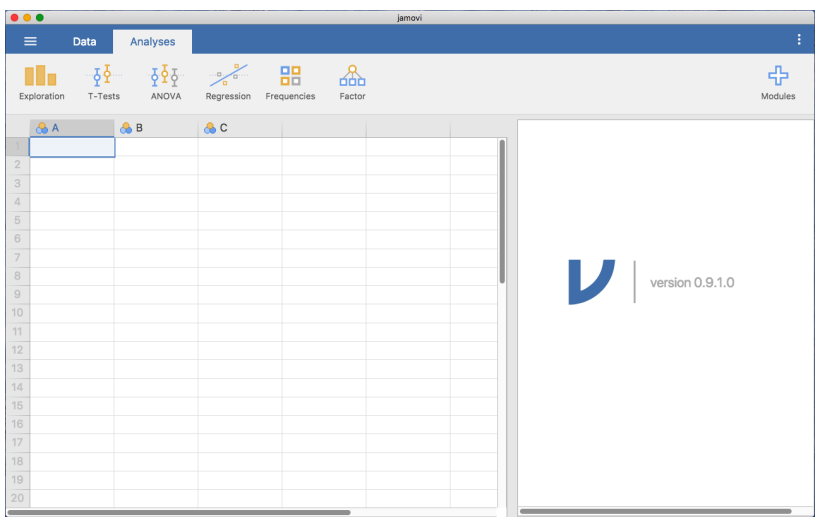
\includegraphics[width=0.9\linewidth]{images/Figure2} \caption{jamovi starts up!}\label{fig:fig3-1}
\end{figure}

To the left is the spreadsheet view, and to the right is where the
results of statistical tests appear. Down the middle is a bar separating
these two regions and this can be dragged to the left or the right to
change their sizes.

It is possible to simply begin typing values into the jamovi spreadsheet
as you would in any other spreadsheet software. Alternatively, existing
data sets in the CSV (.csv) file format can be opened in jamovi.
Additionally, you can easily import SPSS, SAS, Stata and JASP files
directly into jamovi. To open a file select the File tab (three
horizontal lines signify this tab) at the top left hand corner, select
`Open' and then choose from the files listed on 'Browse' depending on
whether you want to open an example or a file stored on your computer.

\hypertarget{analyses}{%
\section{Analyses}\label{analyses}}

Analyses can be selected from the analysis ribbon or menu along the top.
Selecting an analysis will present an `options panel' for that
particular analysis, allowing you to assign different variables to
different parts of the analysis, and select different options. At the
same time, the results for the analysis will appear in the right
`Results panel' and will update in real-time as you make changes to the
options.

When you have the analysis set up correctly you can dismiss the analysis
options by clicking the arrow to the top right of the optional panel. If
you wish to return to these options, you can click on the results that
were produced. In this way, you can return to any analysis that you (or
say, a colleague) created earlier.

If you decide you no longer need a particular analysis, you can remove
it with the results context menu. Right-clicking on the analysis results
will bring up a menu and by selecting `Analysis' and then `Remove' the
analysis can be removed. But more on this later. First, let's take a
more detailed look at the spreadsheet view.

\hypertarget{the-spreadsheet}{%
\section{The spreadsheet}\label{the-spreadsheet}}

In jamovi data is represented in a spreadsheet with each column
representing a `variable' and each row representing a `case' or
`participant'.

\hypertarget{variables}{%
\subsection{Variables}\label{variables}}

The most commonly used variables in jamovi are `Data Variables', these
variables simply contain data either loaded from a data file, or `typed
in' by the user. Data variables can be one of several measurement
levels (Figure \ref{fig:fig3-2}).

\begin{figure}
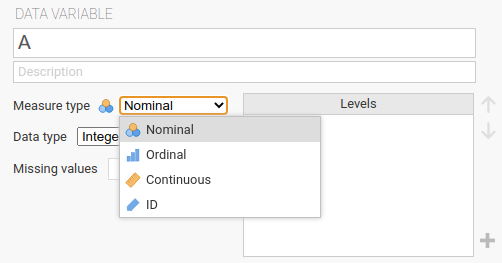
\includegraphics[width=0.9\linewidth]{images/Figure3} \caption{measurement levels}\label{fig:fig3-2}
\end{figure}

These levels are designated by the symbol in the header of the
variable's column. The ID variable type is unique to jamovi. It's
intended for variables that contain identifiers that you would almost
never want to analyse. For example, a persons name, or a participant ID.
Specifying an ID variable type can improve performance when interacting
with very large data sets.

\emph{Nominal} variables are for categorical variables which are text labels,
for example a column called Gender with the values Male and Female would
be nominal. So would a person's name. Nominal variable values can also
have a numeric value. These variables are used most often when importing
data which codes values with numbers rather than text. For example, a
column in a dataset may contain the values 1 for males, and 2 for
females. It is possible to add nice `human-readable' labels to these
values with the variable editor (more on this later).

\emph{Ordinal} variables are like Nominal variables, except the values have a
specific order. An example is a Likert scale with 3 being `strongly
agree' and -3 being `strongly disagree'.

\emph{Continuous} variables are variables which exist on a continuous scale.
Examples might be height or weight. This is also referred to as
`Interval' or `Ratio scale'.

In addition, you can also specify different data types: variables have a
data type of either `Text', `Integer' or `Decimal'.

When starting with a blank spreadsheet and typing values in the variable
type will change automatically depending on the data you enter. This is
a good way to get a feel for which variable types go with which sorts of
data. Similarly, when opening a data file jamovi will try and guess the
variable type from the data in each column. In both cases this automatic
approach may not be correct, and it may be necessary to manually specify
the variable type with the variable editor.

The variable editor can be opened by selecting `Setup' from the data tab
or by double-clicking on the variable column header. The variable editor
allows you to change the name of the variable and, for data variables,
the variable type, the order of the levels, and the label displayed for
each level. Changes can be applied by clicking the `tick' to the top
right. The variable editor can be dismissed by clicking the `Hide'
arrow.

New variables can be inserted or appended to the data set using the
`add' button from the data ribbon. The `add' button also allows the
addition of computed variables.

\hypertarget{computed-variables}{%
\subsection{Computed variables}\label{computed-variables}}

Computed Variables are those which take their value by performing a
computation on other variables. Computed Variables can be used for a
range of purposes, including log transforms, z-scores, sum-scores,
negative scoring and means.

Computed variables can be added to the data set with the `add' button
available on the data tab. This will produce a formula box where you can
specify the formula. The usual arithmetic operators are available. Some
examples of formulas are:

A + B LOG10(len) MEAN(A, B) (dose - VMEAN(dose)) / VSTDEV(dose)

In order, these are the sum of A and B, a log (base 10) transform of
len, the mean of A and B, and the z-score of the variable dose. Figure \ref{fig:fig3-3}
shows the jamovi screen for the new variable computed as the
z-score of dose (from the `Tooth Growth' example data set).

\begin{figure}
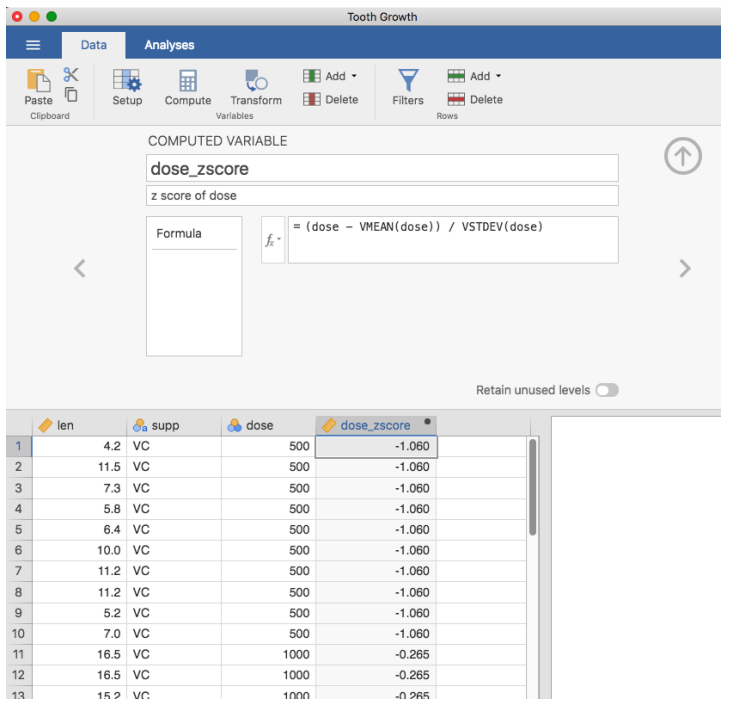
\includegraphics[width=0.9\linewidth]{images/Figure4} \caption{A newly computed variable, the z-score of ‘dose’}\label{fig:fig3-3}
\end{figure}

\hypertarget{v-functions}{%
\subsubsection{V-functions}\label{v-functions}}

Several functions are already available in jamovi and available from the
drop down box labelled fx. A number of functions appear in pairs, one
prefixed with a V and the other not. V functions perform their
calculation on a variable as a whole, where as non-V functions perform
their calculation row by row. For example, MEAN(A, B) will produce the
mean of A and B for each row. Where as VMEAN(A) gives the mean of all
the values in A.

\hypertarget{copy-and-paste}{%
\subsection{Copy and Paste}\label{copy-and-paste}}

jamovi produces nice American Psychological Association (APA) formatted
tables and attractive plots. It is often useful to be able to copy and
paste these, perhaps into a Word document, or into an email to a
colleague. To copy results right click on the object of interest and
from the menu select exactly what you want to copy. The menu allows you
to choose to copy only the image or the entire analysis. Selecting
``copy'' copies the content to the clipboard and this can be pasted into
other programs in the usual way. You can practice this later on when we
do some analyses.

\hypertarget{syntax-mode}{%
\subsection{Syntax mode}\label{syntax-mode}}

jamovi also provides an ``R Syntax Mode''. In this mode jamovi produces
equivalent R code for each analysis. To change to syntax mode, select
the Application menu to the top right of jamovi (a button with three
vertical dots) and click the ``Syntax mode'' checkbox there. You can turn
off syntax mode by clicking this a second time.

In syntax mode analyses continue to operate as before but now they
produce R syntax, and `ascii output' like an R session. Like all results
objects in jamovi, you can right click on these items (including the R
syntax) and copy and paste them, for example into an R session. At
present, the provided R syntax does not include the data import step and
so this must be performed manually in R. There are many resources
explaining how to import data into R and if you are interested we
recommend you take a look at these; just search on the interweb.

\hypertarget{loading-data-in-jamovi}{%
\section{Loading data in jamovi}\label{loading-data-in-jamovi}}

There are several different types of files that are likely to be
relevant to us when doing data analysis. There are two in particular
that are especially important from the perspective of this book:

\begin{itemize}
\item
  \emph{jamovi files} are those with a .omv file extension. This is the
  standard kind of file that jamovi uses to store data, and variables
  and analyses.
\item
  \emph{Comma separated value (csv) files} are those with a .csv file
  extension. These are just regular old text files and they can be
  opened with many different software programs. It's quite typical for
  people to store data in csv files, precisely because they're so
  simple.
\end{itemize}

There are also several other kinds of data file that you might want to
import into jamovi. For instance, you might want to open Microsoft Excel
spreadsheets (.xls files), or data files that have been saved in the
native file formats for other statistics software, such as SPSS or SAS.
Whichever file formats you are using, it's a good idea to create a
folder or folders especially for your jamovi data sets and analyses and
to make sure you keep these backed up regularly.

\begin{figure}
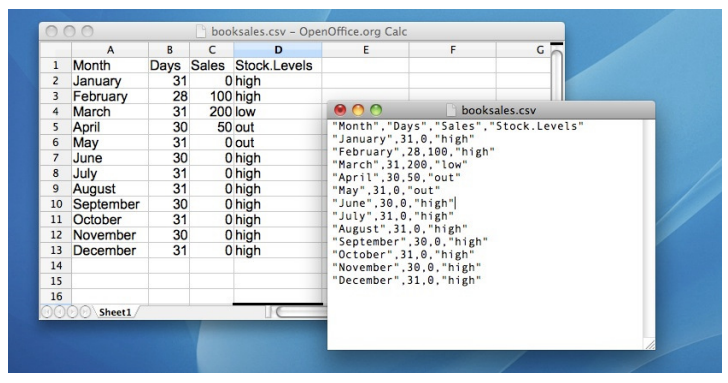
\includegraphics[width=0.9\linewidth]{images/Figure5} \caption{The booksales.csv data file. On the left I have opened the file using a spreadsheet program (OpenOffice), which shows that the file is basically a table. On the right the same file is open in a standard text editor (the TextEdit program on a Mac), which shows how the file is formatted. The entries in the table are wrapped in quote marks and separated by commas}\label{fig:fig3-4}
\end{figure}

\hypertarget{importing-data-from-csv-files}{%
\subsection{Importing data from csv files}\label{importing-data-from-csv-files}}

One quite commonly used data format is the humble ``comma separated
value'' file, also called a csv file, and usually bearing the file
extension .csv. csv files are just plain old-fashioned text files and
what they store is basically just a table of data. This is illustrated
in Figure \ref{fig:fig3-4}, which shows a file called booksales.csv that I've
created. As you can see, each row represents the book sales data for one
month. The first row doesn't contain actual data though, it has the
names of the variables.

It's easy to open csv files in jamovi. From the top left menu (the
button with three parallel lines) choose `Open' and browse to where you
have stored the csv file on your computer. If you're on a Mac, it'll
look like the usual Finder window that you use to choose a file; on
Windows it looks like an Explorer window. An example of what it looks
like on a Mac is shown in Figure \ref{fig:fig3-5}. I'm assuming that you're
familiar with your own computer, so you should have no problem finding
the csv file that you want to import! Find the one you want, then click
on the ``Open'' button.

There are a few things that you can check to make sure that the data
gets imported correctly:

\begin{itemize}
\tightlist
\item
  Heading. Does the first row of the file contain the names for each
  variable - a `header' row? The booksales.csv file has a header, so
  that's a yes.
\item
  Decimal. What character is used to specify the decimal point? In
  English speaking countries this is almost always a period (i.e., .).
  That's not universally true though, many European countries use a
  comma.
\item
  Quote. What character is used to denote a block of text? That's
  usually going to be a double quote mark (``). It is for the
  booksales.csv file.
\end{itemize}

\begin{figure}
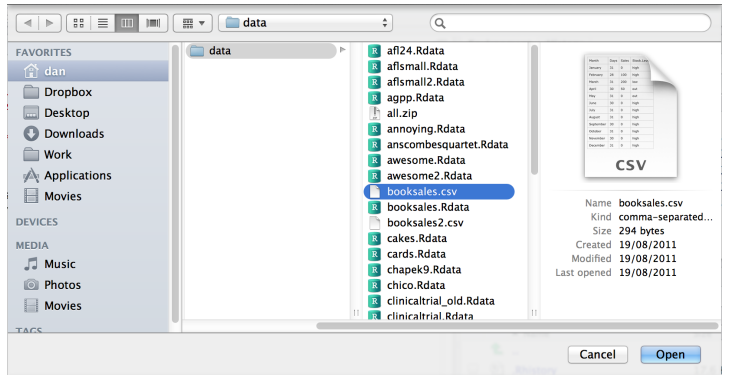
\includegraphics[width=0.9\linewidth]{images/Figure6} \caption{A dialog box on a Mac asking you to select the csv file jamovi should try to import. Mac users will recognise this immediately, it’s the usual way in which a Mac asks you to find a file. Windows users won’t see this, instead they’ll see the usual explorer window that Windows always gives you when it wants you to select a file}\label{fig:fig3-5}
\end{figure}

\hypertarget{importing-unusual-data-files}{%
\section{Importing unusual data files}\label{importing-unusual-data-files}}

Throughout this book I've assumed that your data are stored as a jamovi
.omv file or as a ``properly'' formatted csv file. However, in real life
that's not a terribly plausible assumption to make so I'd better talk
about some of the other possibilities that you might run into.

\hypertarget{loading-data-from-text-files}{%
\subsection{Loading data from text files}\label{loading-data-from-text-files}}

The first thing I should point out is that if your data are saved as a
text file but aren't quite in the proper csv format then there's still a
pretty good chance that jamovi will be able to open it. You just need to
try it and see if it works. Sometimes though you will need to change
some of the formatting. The ones that I've often found myself needing to
change are:

\begin{itemize}
\tightlist
\item
  header. A lot of the time when you're storing data as a csv file the
  first row actually contains the column names and not data. If that's
  not true then it's a good idea to open up the csv file in a
  spreadsheet programme such as Open Office and add the header row
  manually.
\item
  sep. As the name ``comma separated value'' indicates, the values in a
  row of a csv file are usually separated by commas. This isn't
  universal, however. In Europe the decimal point is typically written
  as , instead of . and as a consequence it would be somewhat awkward
  to use , as the separator. Therefore it is not unusual to use ;
  instead of , as the separator. At other times, I've seen a TAB
  character used.
\item
  quote. It's conventional in csv files to include a quoting character
  for textual data. As you can see by looking at the booksales.csv
  file, this is usually a double quote character, ``. But sometimes
  there is no quoting character at all, or you might see a single
  quote mark ' used instead.
\item
  skip. It's actually very common to receive CSV files in which the
  first few rows have nothing to do with the actual data. Instead,
  they provide a human readable summary of where the data came from,
  or maybe they include some technical info that doesn't relate to the
  data.
\item
  missing values. Often you'll get given data with missing values. For
  one reason or another, some entries in the table are missing. The
  data file needs to include a ``special'' value to indicate that the
  entry is missing. By default jamovi assumes that this value is
  99\footnote{You can change the default value for missing values in jamovi from
    the top right menu (three vertical dots), but this only works at the
    time of importing data files into jamovi. The default missing value in
    the dataset should not be a valid number associated with any of the
    variables, e.g.~you could use -9999 as this is unlikely to be a valid
    value.}, for both numeric and text data, so you should
  make sure that, where necessary, all missing values in the csv file
  are replaced with 99 (or -9999; whichever you choose) before opening
  / importing the file into jamovi. Once you have opened / imported
  the file into jamovi all the missing values are converted to blank
  or greyed out cells in the jamovi spreadsheet view. You can also
  change the missing value for each variable as an option in the
  Data - Setup view.
\end{itemize}

\hypertarget{loading-data-from-spss-and-other-statistics-packages}{%
\subsection{Loading data from SPSS (and other statistics packages)}\label{loading-data-from-spss-and-other-statistics-packages}}

The commands listed above are the main ones we'll need for data files in
this book. But in real life we have many more possibilities. For
example, you might want to read data files in from other statistics
programs. Since SPSS is probably the most widely used statistics package
in psychology, it's worth mentioning that jamovi can also import SPSS
data files (file extension .sav). Just follow the instructions above for
how to open a csv file, but this time navigate to the .sav file you want
to import. For SPSS files, jamovi will regard all values as missing if
they are regarded as ``system missing'' files in SPSS. The `Default
missings' value does not seem to work as expected when importing SPSS
files, so be aware of this - you might need another step: import the
SPSS file into jamovi, then export as a csv file before re-opening in
jamovi.\footnote{I know this is a bit of a fudge, but it does work and hopefully
  this will be fixed in a later version of jamovi.}

And that's pretty much it, at least as far as SPSS goes. As far as other
statistical software goes, jamovi can also directly open / import SAS
and STATA files.

\hypertarget{loading-excel-files}{%
\subsection{Loading Excel files}\label{loading-excel-files}}

A different problem is posed by Excel files. Despite years of yelling at
people for sending data to me encoded in a proprietary data format, I
get sent a lot of Excel files. The way to handle Excel files is to open
them up first in Excel or another spreadsheet programme that can handle
Excel files, and then export the data as a csv file before opening /
importing the csv file into jamovi.

\hypertarget{changing-data-from-one-level-to-another}{%
\section{Changing data from one level to another}\label{changing-data-from-one-level-to-another}}

Sometimes you want to change the variable level. This can happen for all
sorts of reasons. Sometimes when you import data from files, it can come
to you in the wrong format. Numbers sometimes get imported as nominal,
text values. Dates may get imported as text. ParticipantID values can
sometimes be read as continuous: nominal values can sometimes be read as
ordinal or even continuous. There's a good chance that sometimes you'll
want to convert a variable from one measurement level into another one.
Or, to use the correct term, you want to \textbf{coerce} the variable from
one class into another.

Earlier we saw how to specify different variable levels, and if you want
to change a variable's measurement level then you can do this in the
jamovi data view for that variable. Just click the check box for the
measurement level you want - continuous, ordinal, or nominal.

\hypertarget{installing-add-on-modules-into-jamovi}{%
\section{Installing add-on modules into jamovi}\label{installing-add-on-modules-into-jamovi}}

A really great feature of jamovi is the ability to install add-on
modules from the jamovi library. These add-on modules have been
developed by the jamovi community, i.e., jamovi users and developers who
have created special software add-ons that do other, usually more
advanced, analyses that go beyond the capabilities of the base jamovi
program.

To install add-on modules, just click on the large \(+\) in the top right
of the jamovi window, select ``jamovi-library'' and then browse through
the various add-on modules that are available. Choose the one(s) you
want, and then install them, as in Figure \ref{fig:fig3-6}. It's that easy. The newly
installed modules can then be accessed from the ``Analyses'' button bar.
Try it\ldots useful add-on modules to install include ''scatr'' (added under
``Descriptives'') and \(R_j\).

\begin{figure}
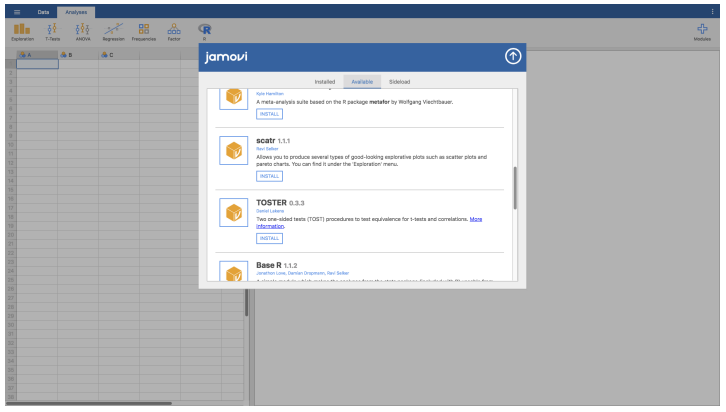
\includegraphics[width=0.9\linewidth]{images/Figure7} \caption{Installing add-on modules in jamovi}\label{fig:fig3-6}
\end{figure}

\hypertarget{quitting-jamovi}{%
\section{Quitting jamovi}\label{quitting-jamovi}}

There's one last thing I should cover in this chapter: how to quit
jamovi. It's not hard, just close the program the same way you would any
other program. However, what you might want to do before you quit is
save your work! There are two parts to this: saving any changes to the
data set, and saving the analyses that you ran.

It is good practice to save any changes to the data set as a \emph{new} data
set. That way you can always go back to the original data. To save any
changes in jamovi, select `Export'\ldots{}`Data' from the main jamovi menu
(button with three horizontal bars in the top left) and create a new
file name for the changed data set.

Alternatively, you can save \emph{both} the changed data and any analyses you
have undertaken by saving as a jamovi file. To do this, from the main
jamovi menu select `Save as' and type in a file name for this `jamovi
file (.omv)'. Remember to save the file in a location where you can find
it again later. I usually create a new folder for specific data sets and
analyses.

\hypertarget{summary-1}{%
\section{Summary}\label{summary-1}}

Every book that tries to teach a new statistical software program to
novices has to cover roughly the same topics, and in roughly the same
order. Ours is no exception, and so in the grand tradition of doing it
just the same way everyone else did it, this chapter covered the
following topics:

\begin{itemize}
\tightlist
\item
  \protect\hyperlink{installing-jamovi}{Installing jamovi}. We downloaded and installed jamovi, and started it up.
\item
  \protect\hyperlink{analyses}{Analyses}. We very briefly oriented to the part of jamovi where
  analyses are done and results appear, but then deferred this until
  later in the book.
\item
  \protect\hyperlink{the-spreadsheet}{The spreadsheet}. We spent more time looking at the spreadsheet part of
  jamovi, and considered different variable types, and how to compute
  new variables.
\item
  \protect\hyperlink{loading-data-in-jamovi}{Loading data in jamovi}. We also saw how to load data files in jamovi.
\item
  \protect\hyperlink{importing-unusual-data-files}{Importing unusual data files}. Then we figured out how to open other data files, from
  different file types.
\item
  \protect\hyperlink{changing-data-from-one-level-to-another}{Changing data from one level to another}. And saw that sometimes we need to coerce data from one
  type to another.
\item
  \protect\hyperlink{installing-add-on-modules-into-jamovi}{Installing add-on modules into jamovi}. Installing add-on modules from the jamovi community
  really extends jamovi capabilities.
\item
  \protect\hyperlink{quitting-jamovi}{Quitting jamovi}. Finally, we looked at good practice in terms of saving
  your data set and analyses when you have finished and are about to
  quit jamovi.
\end{itemize}

We still haven't arrived at anything that resembles data analysis. Maybe
the next Chapter will get us a bit closer!

\begin{center}\rule{0.5\linewidth}{0.5pt}\end{center}

\hypertarget{descriptive-statistics}{%
\chapter{Descriptive statistics}\label{descriptive-statistics}}

Any time that you get a new data set to look at one of the first tasks that you have to do is find ways of summarising the data in a compact, easily understood fashion. This is what \textbf{descriptive statistics} (as opposed to inferential statistics) is all about. In fact, to many people the term ``statistics'' is synonymous with descriptive statistics. It is this topic that we'll consider in this chapter, but before going into any details, let's take a moment to get a sense of why we need descriptive statistics. To do this, let's open the aflsmall\_margins file and see what variables are stored in the file, see Figure \ref{fig:fig4-1}.

\begin{figure}
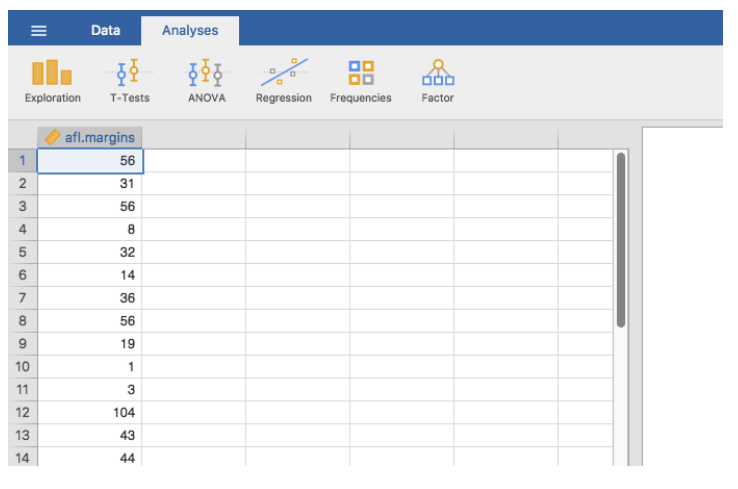
\includegraphics[width=0.9\linewidth]{images/Figure8} \caption{A screenshot of jamovi showing the variables stored in the aflsmallmargins.csv file}\label{fig:fig4-1}
\end{figure}

In fact, there is just one variable here, afl.margins. We'll focus a bit on this variable in this chapter, so I'd better tell you what it is. Unlike most of the data sets in this book, this is actually real data, relating to the Australian Football League (AFL).\footnote{Note for non-Australians: the AFL is an Australian rules football competition. You don't need to know anything about Australian rules in order to follow this section.} The afl.margins variable contains the winning margin (number of points) for all 176 home and away games played during the 2010 season.

This output doesn't make it easy to get a sense of what the data are actually saying. Just ``looking at the data'' isn't a terribly effective way of understanding data. In order to get some idea about what the data are actually saying we need to calculate some descriptive statistics (this chapter) and draw some nice pictures (Chapter 5). Since the descriptive statistics are the easier of the two topics I'll start with those, but nevertheless I'll show you a histogram of the afl.margins data since it should help you get a sense of what the data we're trying to describe actually look like, see Figure \ref{fig:fig4-2}. We'll talk a lot more about how to draw histograms in the section on \protect\hyperlink{histograms}{Histograms} in the next chapter. For now, it's enough to look at the histogram and note that it provides a fairly interpretable representation of the afl.margins data.

\begin{figure}
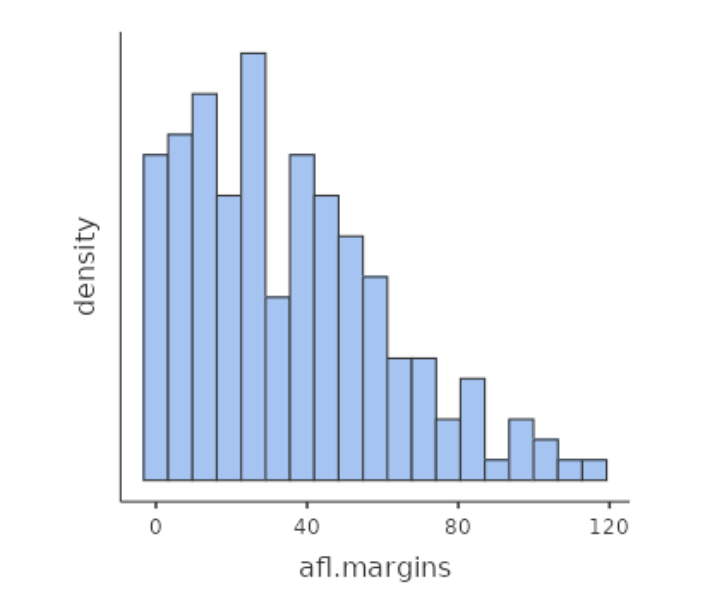
\includegraphics[width=0.9\linewidth]{images/Figure9} \caption{A histogram of the AFL 2010 winning margin data (the afl.margins variable). As you might expect, the larger the winning margin the less frequently you tend to see it}\label{fig:fig4-2}
\end{figure}

\hypertarget{measures-of-central-tendency}{%
\section{Measures of central tendency}\label{measures-of-central-tendency}}

Drawing pictures of the data, as I did in Figure \ref{fig:fig4-2}, is an excellent way to convey the ``gist'' of what the data is trying to tell you. It's often extremely useful to try to condense the data into a few simple ``summary'' statistics. In most situations, the first thing that you'll want to calculate is a measure of \textbf{central tendency}. That is, you'd like to know something about where the ``average'' or ``middle'' of your data lies. The three most commonly used measures are the mean, median and mode. I'll explain each of these in turn, and then discuss when each of them is useful.

\hypertarget{the-mean}{%
\subsection{The mean}\label{the-mean}}

The \textbf{mean} of a set of observations is just a normal, old-fashioned average. Add all of the values up, and then divide by the total number of values. The first five AFL winning margins were 56, 31, 56, 8 and 32, so the mean of these observations is just:

\[
\frac{56 + 31 + 56 + 8 + 32}{5} = \frac{183}{5} = 36.60
\]

Of course, this definition of the mean isn't news to anyone. Averages (i.e., means) are used so often in everyday life that this is pretty familiar stuff. However, since the concept of a mean is something that everyone already understands, I'll use this as an excuse to start introducing some of the mathematical notation that statisticians use to describe this calculation, and talk about how the calculations would be done in jamovi.

The first piece of notation to introduce is \(N\), which we'll use to refer to the number of observations that we're averaging (in this case \(N = 5\)). Next, we need to attach a label to the observations themselves. It's traditional to use X for this, and to use subscripts to indicate which observation we're actually talking about. That is, we'll use \(X_1\) to refer to the first observation, \(X_2\) to refer to the second observation, and so on all the way up to \(X_N\) for the last one. Or, to say the same thing in a slightly more abstract way, we use \(X_i\) to refer to the i-th observation. Just to make sure we're clear on the notation, Table \ref{tab:tab4-1} lists the 5 observations in the afl.margins variable, along with the mathematical symbol used to refer to it and the actual value that the observation corresponds to:

 
  \providecommand{\huxb}[2]{\arrayrulecolor[RGB]{#1}\global\arrayrulewidth=#2pt}
  \providecommand{\huxvb}[2]{\color[RGB]{#1}\vrule width #2pt}
  \providecommand{\huxtpad}[1]{\rule{0pt}{#1}}
  \providecommand{\huxbpad}[1]{\rule[-#1]{0pt}{#1}}

\begin{table}[ht]
\begin{centerbox}
\begin{threeparttable}
\setlength{\tabcolsep}{0pt}
\begin{tabular}{l l l}


\hhline{>{\huxb{0, 0, 0}{0.4}}->{\huxb{0, 0, 0}{0.4}}->{\huxb{0, 0, 0}{0.4}}-}
\arrayrulecolor{black}

\multicolumn{1}{!{\huxvb{0, 0, 0}{0}}c!{\huxvb{0, 0, 0}{0}}}{\cellcolor[RGB]{242, 242, 242}\huxtpad{6pt + 1em}\centering \hspace{0pt} \textbf{the observation} \hspace{6pt}\huxbpad{6pt}} &
\multicolumn{1}{c!{\huxvb{0, 0, 0}{0}}}{\cellcolor[RGB]{242, 242, 242}\huxtpad{6pt + 1em}\centering \hspace{6pt} \textbf{its symbol} \hspace{6pt}\huxbpad{6pt}} &
\multicolumn{1}{c!{\huxvb{0, 0, 0}{0}}}{\cellcolor[RGB]{242, 242, 242}\huxtpad{6pt + 1em}\centering \hspace{6pt} \textbf{the observed value} \hspace{0pt}\huxbpad{6pt}} \tabularnewline[-0.5pt]


\hhline{>{\huxb{0, 0, 0}{0.4}}->{\huxb{0, 0, 0}{0.4}}->{\huxb{0, 0, 0}{0.4}}-}
\arrayrulecolor{black}

\multicolumn{1}{!{\huxvb{0, 0, 0}{0}}c!{\huxvb{0, 0, 0}{0}}}{\huxtpad{6pt + 1em}\centering \hspace{0pt} winning margin, game 1 \hspace{6pt}\huxbpad{6pt}} &
\multicolumn{1}{c!{\huxvb{0, 0, 0}{0}}}{\huxtpad{6pt + 1em}\centering \hspace{6pt} $\backslash$(X\_1$\backslash$) \hspace{6pt}\huxbpad{6pt}} &
\multicolumn{1}{c!{\huxvb{0, 0, 0}{0}}}{\huxtpad{6pt + 1em}\centering \hspace{6pt} 56 points \hspace{0pt}\huxbpad{6pt}} \tabularnewline[-0.5pt]


\hhline{}
\arrayrulecolor{black}

\multicolumn{1}{!{\huxvb{0, 0, 0}{0}}c!{\huxvb{0, 0, 0}{0}}}{\cellcolor[RGB]{242, 242, 242}\huxtpad{6pt + 1em}\centering \hspace{0pt} winning margin, game 2 \hspace{6pt}\huxbpad{6pt}} &
\multicolumn{1}{c!{\huxvb{0, 0, 0}{0}}}{\cellcolor[RGB]{242, 242, 242}\huxtpad{6pt + 1em}\centering \hspace{6pt} $\backslash$(X\_2$\backslash$) \hspace{6pt}\huxbpad{6pt}} &
\multicolumn{1}{c!{\huxvb{0, 0, 0}{0}}}{\cellcolor[RGB]{242, 242, 242}\huxtpad{6pt + 1em}\centering \hspace{6pt} 31 points \hspace{0pt}\huxbpad{6pt}} \tabularnewline[-0.5pt]


\hhline{}
\arrayrulecolor{black}

\multicolumn{1}{!{\huxvb{0, 0, 0}{0}}c!{\huxvb{0, 0, 0}{0}}}{\huxtpad{6pt + 1em}\centering \hspace{0pt} winning margin, game 3 \hspace{6pt}\huxbpad{6pt}} &
\multicolumn{1}{c!{\huxvb{0, 0, 0}{0}}}{\huxtpad{6pt + 1em}\centering \hspace{6pt} $\backslash$(X\_3$\backslash$) \hspace{6pt}\huxbpad{6pt}} &
\multicolumn{1}{c!{\huxvb{0, 0, 0}{0}}}{\huxtpad{6pt + 1em}\centering \hspace{6pt} 56 points \hspace{0pt}\huxbpad{6pt}} \tabularnewline[-0.5pt]


\hhline{}
\arrayrulecolor{black}

\multicolumn{1}{!{\huxvb{0, 0, 0}{0}}c!{\huxvb{0, 0, 0}{0}}}{\cellcolor[RGB]{242, 242, 242}\huxtpad{6pt + 1em}\centering \hspace{0pt} winning margin, game 4 \hspace{6pt}\huxbpad{6pt}} &
\multicolumn{1}{c!{\huxvb{0, 0, 0}{0}}}{\cellcolor[RGB]{242, 242, 242}\huxtpad{6pt + 1em}\centering \hspace{6pt} $\backslash$(X\_4$\backslash$) \hspace{6pt}\huxbpad{6pt}} &
\multicolumn{1}{c!{\huxvb{0, 0, 0}{0}}}{\cellcolor[RGB]{242, 242, 242}\huxtpad{6pt + 1em}\centering \hspace{6pt} 8 points \hspace{0pt}\huxbpad{6pt}} \tabularnewline[-0.5pt]


\hhline{}
\arrayrulecolor{black}

\multicolumn{1}{!{\huxvb{0, 0, 0}{0}}c!{\huxvb{0, 0, 0}{0}}}{\huxtpad{6pt + 1em}\centering \hspace{0pt} winning margin, game 5 \hspace{6pt}\huxbpad{6pt}} &
\multicolumn{1}{c!{\huxvb{0, 0, 0}{0}}}{\huxtpad{6pt + 1em}\centering \hspace{6pt} $\backslash$(X\_5$\backslash$) \hspace{6pt}\huxbpad{6pt}} &
\multicolumn{1}{c!{\huxvb{0, 0, 0}{0}}}{\huxtpad{6pt + 1em}\centering \hspace{6pt} 32 points \hspace{0pt}\huxbpad{6pt}} \tabularnewline[-0.5pt]


\hhline{>{\huxb{0, 0, 0}{0.4}}->{\huxb{0, 0, 0}{0.4}}->{\huxb{0, 0, 0}{0.4}}-}
\arrayrulecolor{black}
\end{tabular}\captionsetup{justification=raggedright,singlelinecheck=off}
\caption{\label{tab:tab4-1} Observations in the afl.margins variable}
 
\end{threeparttable}\par\end{centerbox}

\end{table}
 

{{[}Option: statistical formulae{]}}\footnote{{Okay, now let's try to write a formula for the mean. By tradition, we use \(\bar{X}\) as the notation for the mean. So the calculation for the mean could be expressed using the following formula: \[\bar{X}=\frac{X_1 + X_2 ... + X_{N-1} + X_{N}}{N}\] This formula is entirely correct but it's terribly long, so we make use of the summation symbol \(\sum\) to shorten it.\(^a\) If I want to add up the first five observations I could write out the sum the long way, \(X_1 + X_2 + X_3 + X_4 + X_5\) or I could use the summation symbol to shorten it to this: \[\sum_{i=1}^{5} X_i\] Taken literally, this could be read as ``the sum, taken over all i values from 1 to 5, of the value \(X_i\)''. But basically what it means is ``add up the first five observations''. In any case, we can use this notation to write out the formula for the mean, which looks like this: \[\bar{X}=\frac{1}{N}\sum_{i=1}^{N}X_i\] In all honesty, I can't imagine that all this mathematical notation helps clarify the concept of the mean at all. In fact, it's really just a fancy way of writing out the same thing I said in words: add all the values up and then divide by the total number of items. However, that's not really the reason I went into all that detail. My goal was to try to make sure that everyone reading this book is clear on the notation that we'll be using throughout the book: \(\bar{X}\) for the mean, \(\sum\) for the idea of summation, \(X_i\) for the ith observation, and \(N\) for the total number of observations. We're going to be re-using these symbols a fair bit so it's important that you understand them well enough to be able to ``read'' the equations, and to be able to see that it's just saying ``add up lots of things and then divide by another thing''. ---\(^a\) \emph{The choice to use} \(\sum\) to denote summation isn't arbitrary. It's the Greek upper case letter sigma, which is the analogue of the letter \(S\) in that alphabet. Similarly, there's an equivalent symbol used to denote the multiplication of lots of numbers, because multiplications are also called ``products'' we use the \(\prod\) symbol for this (the Greek upper case pi, which is the analogue of the letter \(P\).}}

\hypertarget{calculating-the-mean-in-jamovi}{%
\subsection{Calculating the mean in jamovi}\label{calculating-the-mean-in-jamovi}}

Okay, that's the maths. So how do we get the magic computing box to do the work for us? When the number of observations starts to become large it's much easier to do these sorts of calculations using a computer. To calculate the mean using all the data we can use jamovi. The first step is to click on the `Exploration' button and then click `Descriptives'. Then you can highlight the afl.margins variable and click the `right arrow' to move it across into the `Variables box'. As soon as you do that a Table appears on the right hand side of the screen containing default `Descriptives' information; see Figure \ref{fig:fig4-3}.

\begin{figure}
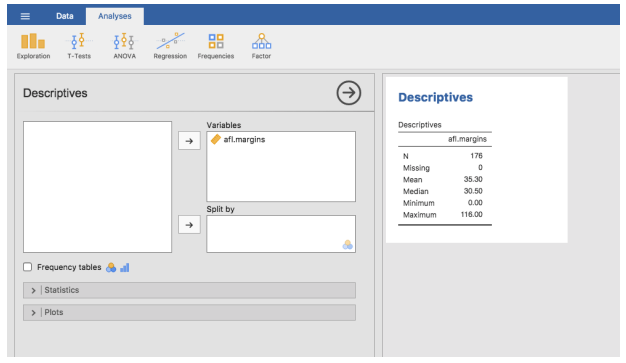
\includegraphics[width=0.9\linewidth]{images/Figure10} \caption{Default descriptives for the AFL 2010 winning margin data (the afl.margins variable)}\label{fig:fig4-3}
\end{figure}

As you can see in Figure \ref{fig:fig4-3}, the mean value for the afl.margins variable is 35.30. Other information presented includes the total number of observations (N=176), the number of missing values (none), and the Median, Minimum and Maximum values for the variable.

\hypertarget{the-median}{%
\subsection{The median}\label{the-median}}

The second measure of central tendency that people use a lot is the \textbf{median}, and it's even easier to describe than the mean. The median of a set of observations is just the middle value. As before let's imagine we were interested only in the first 5 AFL winning margins: \(56\), \(31\), \(56\), \(8\) and \(32\). To figure out the median we sort these numbers into ascending order:

8, 31, \textbf{32}, 56, 56

From inspection, it's obvious that the median value of these 5 observations is 32 since that's the middle one in the sorted list (I've put it in bold to make it even more obvious). Easy stuff. But what should we do if we are interested in the first 6 games rather than the first 5? Since the sixth game in the season had a winning margin of 14 points, our sorted list is now

8, \textbf{31}, \textbf{32}, 56, 56

and there are two middle numbers, 31 and 32. The median is defined as the average of those two numbers, which is of course 31.5. As before, it's very tedious to do this by hand when you've got lots of numbers. In real life, of course, no-one actually calculates the median by sorting the data and then looking for the middle value. In real life we use a computer to do the heavy lifting for us, and jamovi has provided us with a Median value of 30.50 for the afl.margins variable (Figure \ref{fig:fig4-3}.

\hypertarget{mean-or-median-whats-the-difference}{%
\subsection{Mean or median? What's the difference?}\label{mean-or-median-whats-the-difference}}

Knowing how to calculate means and medians is only a part of the story. You also need to understand what each one is saying about the data, and what that implies for when you should use each one. This is illustrated in \protect\hyperlink{Fig4.4}{Figure 4.4}. The mean is kind of like the ``centre of gravity'' of the data set, whereas the median is the ``middle value'' in the data. What this implies, as far as which one you should use, depends a little on what type of data you've got and what you're trying to achieve. As a rough guide:

\begin{itemize}
\tightlist
\item
  If your data are nominal scale you probably shouldn't be using either the mean or the median. Both the mean and the median rely on the idea that the numbers assigned to values are meaningful. If the numbering scheme is arbitrary then it's probably best to use the \protect\hyperlink{mode}{Mode} instead.
\item
  If your data are ordinal scale you're more likely to want to use the median than the mean. The median only makes use of the order information in your data (i.e., which numbers are bigger) but doesn't depend on the precise numbers involved. That's exactly the situation that applies when your data are ordinal scale. The mean, on the other hand, makes use of the precise numeric values assigned to the observations, so it's not really appropriate for ordinal data.
\item
  For interval and ratio scale data either one is generally acceptable. Which one you pick depends a bit on what you're trying to achieve. The mean has the advantage that it uses all the information in the data (which is useful when you don't have a lot of data). But it's very sensitive to extreme, outlying values.
\end{itemize}

Let's expand on that last part a little. One consequence is that there are systematic differences between the mean and the median when the histogram is asymmetric (\protect\hyperlink{skew-and-kurtosis}{Skew and kurtosis}). This is illustrated in Figure \ref{fig:fig4-4}. Notice that the median (right hand side) is located closer to the ``body'' of the histogram, whereas the mean (left hand side) gets dragged towards the ``tail'' (where the extreme values are). To give a concrete example, suppose Bob (income \$50,000), Kate (income \$60,000) and Jane (income \$65,000) are sitting at a table. The average income at the table is \$58,333 and the median income is \$60,000. Then Bill sits down with them (income \$100,000,000). The average income has now jumped to \$25,043,750 but the median rises only to \$62,500. If you're interested in looking at the overall income at the table the mean might be the right answer. But if you're interested in what counts as a typical income at the table the median would be a better choice here.

\begin{figure}
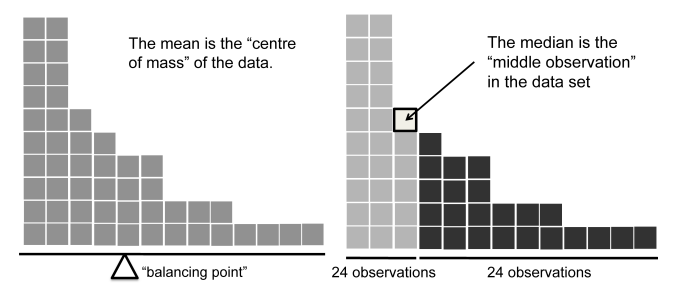
\includegraphics[width=0.9\linewidth]{images/Figure11} \caption{An illustration of the difference between how the mean and the median should be interpreted. The mean is basically the 'centre of gravity' of the data set. If you imagine that the histogram of the data is a solid object, then the point on which you could balance it (as if on a see-saw) is the mean. In contrast, the median is the middle observation, with half of the observations smaller and half of the observations larger}\label{fig:fig4-4}
\end{figure}

\hypertarget{a-real-life-example}{%
\subsection{A real life example}\label{a-real-life-example}}

To try to get a sense of why you need to pay attention to the differences between the mean and the median let's consider a real life example. Since I tend to mock journalists for their poor scientific and statistical knowledge, I should give credit where credit is due. This is an excellent article on the ABC news website\footnote{\url{www.abc.net.au/news/stories/2010/09/24/3021480.htm}} from 24 September, 2010:

\begin{quote}
Senior Commonwealth Bank executives have travelled the world in the past couple of weeks with a presentation showing how Australian house prices, and the key price to income ratios, compare favourably with similar countries. ``Housing affordability has actually been going sideways for the last five to six years,'' said Craig James, the chief economist of the bank's trading arm, CommSec.
\end{quote}

This probably comes as a huge surprise to anyone with a mortgage, or who wants a mortgage, or pays rent, or isn't completely oblivious to what's been going on in the Australian housing market over the last several years. Back to the article:

\begin{quote}
CBA has waged its war against what it believes are housing doomsayers with graphs, numbers and international comparisons. In its presentation, the bank rejects arguments that Australia's housing is relatively expensive compared to incomes. It says Australia's house price to household income ratio of 5.6 in the major cities, and 4.3 nationwide, is comparable to many other developed nations. It says San Francisco and New York have ratios of 7, Auckland's is 6.7, and Vancouver comes in at 9.3.
\end{quote}

More excellent news! Except, the article goes on to make the observation that:

\begin{quote}
Many analysts say that has led the bank to use misleading figures and comparisons. If you go to page four of CBA's presentation and read the source information at the bottom of the graph and table, you would notice there is an additional source on the international comparison -- Demographia. However, if the Commonwealth Bank had also used Demographia's analysis of Australia's house price to income ratio, it would have come up with a figure closer to 9 rather than 5.6 or 4.3
\end{quote}

That's, um, a rather serious discrepancy. One group of people say 9, another says 4-5. Should we just split the difference and say the truth lies somewhere in between? Absolutely not! This is a situation where there is a right answer and a wrong answer. Demographia is correct, and the Commonwealth Bank is wrong. As the article points out:

\begin{quote}
{[}An{]} obvious problem with the Commonwealth Bank's domestic price to income figures is they compare average incomes with median house prices (unlike the Demographia figures that compare median incomes to median prices). The median is the mid-point, effectively cutting out the highs and lows, and that means the average is generally higher when it comes to incomes and asset prices, because it includes the earnings of Australia's wealthiest people. To put it another way: the Commonwealth Bank's figures count Ralph Norris' multi-million dollar pay packet on the income side, but not his (no doubt) very expensive house in the property price figures, thus understating the house price to income ratio for middle-income Australians.
\end{quote}

Couldn't have put it better myself. The way that Demographia calculated the ratio is the right thing to do. The way that the Bank did it is incorrect. As for why an extremely quantitatively sophisticated organisation such as a major bank made such an elementary mistake, well\ldots{} I can't say for sure since I have no special insight into their thinking. But the article itself does happen to mention the following facts, which may or may not be relevant:

\begin{quote}
{[}As{]} Australia's largest home lender, the Commonwealth Bank has one of the biggest vested interests in house prices rising. It effectively owns a massive swathe of Australian housing as security for its home loans as well as many small business loans.
\end{quote}

My, my.

\hypertarget{mode}{%
\subsection{Mode}\label{mode}}

The mode of a sample is very simple. It is the value that occurs most frequently. We can illustrate the mode using a different AFL variable: who has played in the most finals? Open the aflsmall finalists file and take a look at the afl.finalists variable, see Figure \ref{fig:fig4-5}. This variable contains the names of all 400 teams that played in all 200 finals matches played during the period 1987 to 2010.

What we could do is read through all 400 entries and count the number of occasions on which each team name appears in our list of finalists, thereby producing a \textbf{frequency table}. However, that would be mindless and boring: exactly the sort of task that computers are great at. So let's use jamovi to do this for us. Under `Exploration' - `Descriptives' click the small check box labelled `Frequency tables' and you should get something like Figure \ref{fig:fig4-6}.

Now that we have our frequency table we can just look at it and see that, over the 24 years for which we have data, Geelong has played in more finals than any other team. Thus, the mode of the afl.finalists data is ``Geelong''. We can see that Geelong (39 finals) played in more finals than any other team during the 1987-2010 period. It's also worth noting that in the `Descriptives' Table no results are calculated for Mean, Median, Minimum or Maximum. This is because the afl.finalists variable is a nominal text variable so it makes no sense to calculate these values.

\begin{figure}
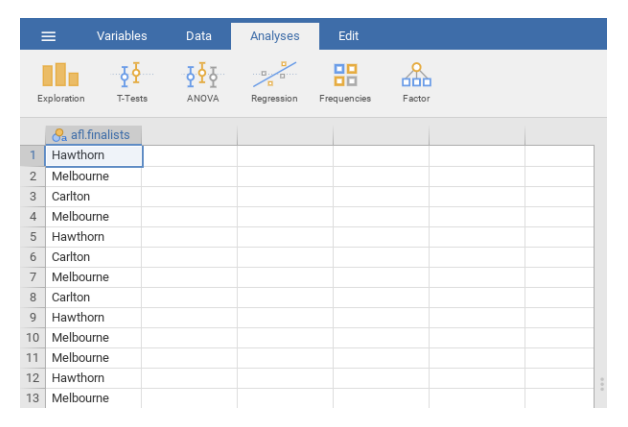
\includegraphics[width=0.9\linewidth]{images/Figure12} \caption{A screenshot of jamovi showing the variables stored in the aflsmall finalists.csv file}\label{fig:fig4-5}
\end{figure}

\begin{figure}
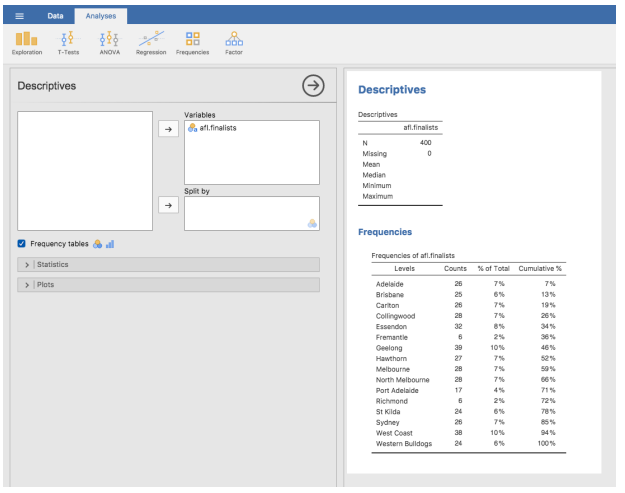
\includegraphics[width=0.9\linewidth]{images/Figure13} \caption{A screenshot of jamovi showing the frequency table for the afl.finalists variable}\label{fig:fig4-6}
\end{figure}

One last point to make regarding the mode. Whilst the mode is most often calculated when you have nominal data, because means and medians are useless for those sorts of variables, there are some situations in which you really do want to know the mode of an ordinal, interval or ratio scale variable. For instance, let's go back to our afl.margins variable. This variable is clearly ratio scale (if it's not clear to you, it may help to re-read the section on \protect\hyperlink{scales-of-measurement}{Scales of measurement}), and so in most situations the mean or the median is the measure of central tendency that you want. But consider this scenario: a friend of yours is offering a bet and they pick a football game at random. Without knowing who is playing you have to guess the exact winning margin. If you guess correctly you win \$50. If you don't you lose \$1. There are no consolation prizes for ``almost'' getting the right answer. You have to guess exactly the right margin. For this bet, the mean and the median are completely useless to you. It is the mode that you should bet on. To calculate the mode for the afl.margins variable in jamovi, go back to that data set and on the `Exploration' - `Descriptives' screen you will see you can expand the section marked `Statistics'. Click on the checkbox marked `Mode' and you will see the modal value presented in the `Descriptives' Table, as in Figure \ref{fig:fig4-7}. So the 2010 data suggest you should bet on a 3 point margin.

\begin{figure}
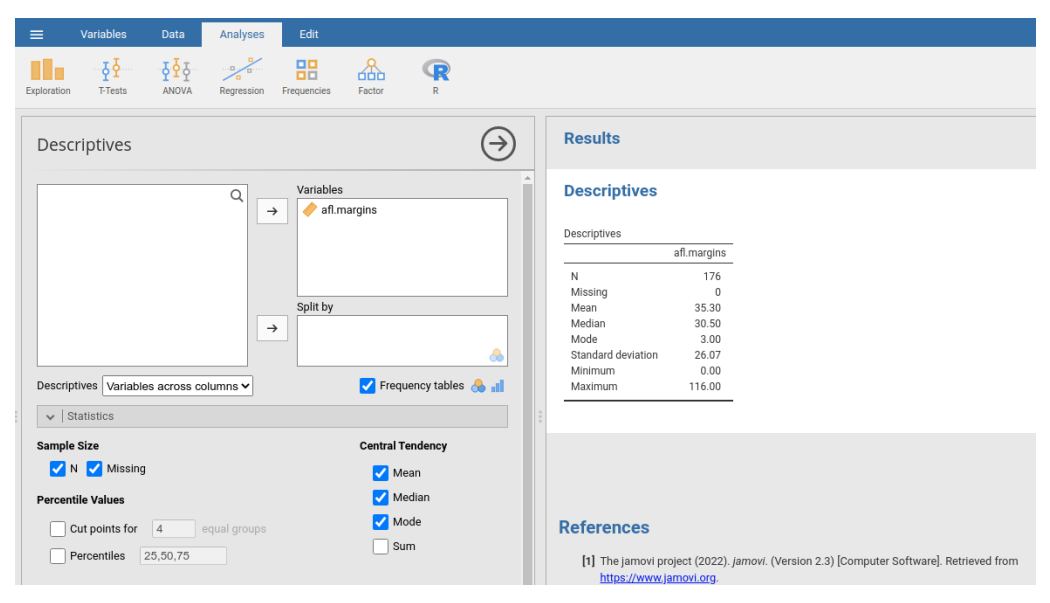
\includegraphics[width=0.9\linewidth]{images/Figure14} \caption{A screenshot of jamovi showing the modal value for the afl.margins variable}\label{fig:fig4-7}
\end{figure}

\hypertarget{measures-of-variability}{%
\section{Measures of variability}\label{measures-of-variability}}

The statistics that we've discussed so far all relate to central tendency. That is, they all talk about which values are ``in the middle'' or ``popular'' in the data. However, central tendency is not the only type of summary statistic that we want to calculate. The second thing that we really want is a measure of the \textbf{variability} of the data. That is, how ``spread out'' are the data? How ``far'' away from the mean or median do the observed values tend to be? For now, let's assume that the data are interval or ratio scale, and we'll continue to use the afl.margins data. We'll use this data to discuss several different measures of spread, each with different strengths and weaknesses.

\hypertarget{range}{%
\subsection{Range}\label{range}}

The statistics that we've discussed so far all relate to central tendency. That is, they all talk about which values are ``in the middle'' or ``popular'' in the data. However, central tendency is not the only type of summary statistic that we want to calculate. The second thing that we really want is a measure of the \textbf{variability} of the data. That is, how ``spread out'' are the data? How ``far'' away from the mean or median do the observed values tend to be? For now, let's assume that the data are interval or ratio scale, and we'll continue to use the afl.margins data. We'll use this data to discuss several different measures of spread, each with different strengths and weaknesses.

The \textbf{range} of a variable is very simple. It's the biggest value minus the smallest value. For the AFL winning margins data the maximum value is 116 and the minimum value is 0. Although the range is the simplest way to quantify the notion of ``variability'', it's one of the worst. Recall from our discussion of the mean that we want our summary measure to be robust. If the data set has one or two extremely bad values in it we'd like our statistics to not be unduly influenced by these cases. For example, in a variable containing very extreme outliers

-100, 2, 3, 4, 5, 6, 7, 8, 9, 10

it is clear that the range is not robust. This variable has a range of 110 but if the outlier were removed we would have a range of only 8.

\hypertarget{interquartile-range}{%
\subsection{Interquartile range}\label{interquartile-range}}

The \textbf{interquartile range} (IQR) is like the range, but instead of the difference between the biggest and smallest value the difference between the 25th percentile and the 75th percentile is taken. If you don't already know what a \textbf{percentile} is, the 10th percentile of a data set is the smallest number x such that 10\% of the data is less than x. In fact, we've already come across the idea. The median of a data set is its 50th percentile! In jamovi you can easily specify the 25th, 50th and 75th percentiles by clicking the checkbox `Quartiles' in the `Exploration' - `Descriptives' - `Statistics' screen.

And not surprisingly, in Figure \ref{fig:fig4-8} the 50th percentile is the same as the median value. And, by noting that \(50.50 - 12.75 = 37.75\), we can see that the interquartile range for the 2010 AFL winning margins data is 37.75. While it's obvious how to interpret the range it's a little less obvious how to interpret the IQR. The simplest way to think about it is like this: the interquartile range is the range spanned by the ``middle half'' of the data. That is, one quarter of the data falls below the 25th percentile and one quarter of the data is above the 75th percentile, leaving the ``middle half'' of the data lying in between the two. And the IQR is the range covered by that middle half.

\begin{figure}
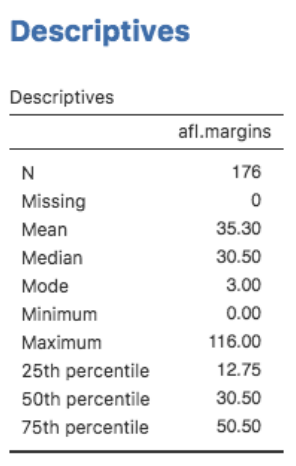
\includegraphics[width=0.5\linewidth]{images/Figure15} \caption{A screenshot of jamovi showing the Quartiles for the afl.margins variable}\label{fig:fig4-8}
\end{figure}

\hypertarget{mean-absolute-deviation}{%
\subsection{Mean absolute deviation}\label{mean-absolute-deviation}}

The two measures we've looked at so far, the range and the interquartile range, both rely on the idea that we can measure the spread of the data by looking at the percentiles of the data. However, this isn't the only way to think about the problem. A different approach is to select a meaningful reference point (usually the mean or the median) and then report the ``typical'' deviations from that reference point. What do we mean by ``typical'' deviation? Usually, this is the mean or median value of these deviations. In practice, this leads to two different measures: the ``mean absolute deviation'' (from the mean) and the ``median absolute deviation'' (from the median). From what I've read, the measure based on the median seems to be used in statistics and does seem to be the better of the two. But to be honest I don't think I've seen it used much in psychology. The measure based on the mean does occasionally show up in psychology though. In this section I'll talk about the first one, and I'll come back to talk about the second one later.

Since the previous paragraph might sound a little abstract, let's go through the \textbf{mean absolute deviation} from the mean a little more slowly. One useful thing about this measure is that the name actually tells you exactly how to calculate it. Let's think about our AFL winning margins data, and once again we'll start by pretending that there are only 5 games in total, with winning margins of 56, 31, 56, 8 and 32. Since our calculations rely on an examination of the deviation from some reference point (in this case the mean), the first thing we need to calculate is the mean, \(\bar{X}\). For these five observations, our mean is \(\bar{X} = 36.6\). The next step is to convert each of our observations \(X_i\) into a deviation score. We do this by calculating the difference between the observation \(X_i\) and the mean \(\bar{X}\). That is, the deviation score is defined to be \(X_i - \bar{X}\). For the first observation in our sample, this is equal to \(56 - 36.6 = 19.4\). Okay, that's simple enough. The next step in the process is to convert these deviations to absolute deviations, and we do this by converting any negative values to positive ones. Mathematically, we would denote the absolute value of \(-3\) as \(\mid -3 \mid\), and so we say that \(\mid -3 \mid = 3\). We use the absolute value here because we don't really care whether the value is higher than the mean or lower than the mean, we're just interested in how close it is to the mean. To help make this process as obvious as possible, Table \ref{tab:tab4-2} shows these calculations for all five observations.

 
  \providecommand{\huxb}[2]{\arrayrulecolor[RGB]{#1}\global\arrayrulewidth=#2pt}
  \providecommand{\huxvb}[2]{\color[RGB]{#1}\vrule width #2pt}
  \providecommand{\huxtpad}[1]{\rule{0pt}{#1}}
  \providecommand{\huxbpad}[1]{\rule[-#1]{0pt}{#1}}

\begin{table}[ht]
\begin{centerbox}
\begin{threeparttable}
\setlength{\tabcolsep}{0pt}
\begin{tabular}{l l l l l}


\hhline{>{\huxb{0, 0, 0}{0.4}}->{\huxb{0, 0, 0}{0.4}}->{\huxb{0, 0, 0}{0.4}}->{\huxb{0, 0, 0}{0.4}}->{\huxb{0, 0, 0}{0.4}}-}
\arrayrulecolor{black}

\multicolumn{1}{!{\huxvb{0, 0, 0}{0}}c!{\huxvb{0, 0, 0}{0}}}{\cellcolor[RGB]{242, 242, 242}\huxtpad{6pt + 1em}\centering \hspace{0pt} \textbf{English} \hspace{6pt}\huxbpad{6pt}} &
\multicolumn{1}{c!{\huxvb{0, 0, 0}{0}}}{\cellcolor[RGB]{242, 242, 242}\huxtpad{6pt + 1em}\centering \hspace{6pt} \textbf{notation} \hspace{6pt}\huxbpad{6pt}} &
\multicolumn{1}{c!{\huxvb{0, 0, 0}{0}}}{\cellcolor[RGB]{242, 242, 242}\huxtpad{6pt + 1em}\centering \hspace{6pt} \textbf{value} \hspace{6pt}\huxbpad{6pt}} &
\multicolumn{1}{c!{\huxvb{0, 0, 0}{0}}}{\cellcolor[RGB]{242, 242, 242}\huxtpad{6pt + 1em}\centering \hspace{6pt} \textbf{deviation from mean} \hspace{6pt}\huxbpad{6pt}} &
\multicolumn{1}{c!{\huxvb{0, 0, 0}{0}}}{\cellcolor[RGB]{242, 242, 242}\huxtpad{6pt + 1em}\centering \hspace{6pt} \textbf{absolute deviation} \hspace{0pt}\huxbpad{6pt}} \tabularnewline[-0.5pt]


\hhline{>{\huxb{0, 0, 0}{0.4}}->{\huxb{0, 0, 0}{0.4}}->{\huxb{0, 0, 0}{0.4}}->{\huxb{0, 0, 0}{0.4}}->{\huxb{0, 0, 0}{0.4}}-}
\arrayrulecolor{black}

\multicolumn{1}{!{\huxvb{0, 0, 0}{0}}c!{\huxvb{0, 0, 0}{0}}}{\huxtpad{6pt + 1em}\centering \hspace{0pt} notation: \hspace{6pt}\huxbpad{6pt}} &
\multicolumn{1}{c!{\huxvb{0, 0, 0}{0}}}{\huxtpad{6pt + 1em}\centering \hspace{6pt} $\backslash$(i$\backslash$) \hspace{6pt}\huxbpad{6pt}} &
\multicolumn{1}{c!{\huxvb{0, 0, 0}{0}}}{\huxtpad{6pt + 1em}\centering \hspace{6pt} $\backslash$(X\_i$\backslash$) \hspace{6pt}\huxbpad{6pt}} &
\multicolumn{1}{c!{\huxvb{0, 0, 0}{0}}}{\huxtpad{6pt + 1em}\centering \hspace{6pt} $\backslash$(X\_i - $\backslash$bar\{X\} $\backslash$) \hspace{6pt}\huxbpad{6pt}} &
\multicolumn{1}{c!{\huxvb{0, 0, 0}{0}}}{\huxtpad{6pt + 1em}\centering \hspace{6pt} $\backslash$( $\backslash$mid X\_i - $\backslash$bar\{X\} $\backslash$mid $\backslash$) \hspace{0pt}\huxbpad{6pt}} \tabularnewline[-0.5pt]


\hhline{}
\arrayrulecolor{black}

\multicolumn{1}{!{\huxvb{0, 0, 0}{0}}c!{\huxvb{0, 0, 0}{0}}}{\cellcolor[RGB]{242, 242, 242}\huxtpad{6pt + 1em}\centering \hspace{0pt}  \hspace{6pt}\huxbpad{6pt}} &
\multicolumn{1}{c!{\huxvb{0, 0, 0}{0}}}{\cellcolor[RGB]{242, 242, 242}\huxtpad{6pt + 1em}\centering \hspace{6pt} 1 \hspace{6pt}\huxbpad{6pt}} &
\multicolumn{1}{c!{\huxvb{0, 0, 0}{0}}}{\cellcolor[RGB]{242, 242, 242}\huxtpad{6pt + 1em}\centering \hspace{6pt} 56 \hspace{6pt}\huxbpad{6pt}} &
\multicolumn{1}{c!{\huxvb{0, 0, 0}{0}}}{\cellcolor[RGB]{242, 242, 242}\huxtpad{6pt + 1em}\centering \hspace{6pt} 19.4 \hspace{6pt}\huxbpad{6pt}} &
\multicolumn{1}{c!{\huxvb{0, 0, 0}{0}}}{\cellcolor[RGB]{242, 242, 242}\huxtpad{6pt + 1em}\centering \hspace{6pt} 19.4 \hspace{0pt}\huxbpad{6pt}} \tabularnewline[-0.5pt]


\hhline{}
\arrayrulecolor{black}

\multicolumn{1}{!{\huxvb{0, 0, 0}{0}}c!{\huxvb{0, 0, 0}{0}}}{\huxtpad{6pt + 1em}\centering \hspace{0pt}  \hspace{6pt}\huxbpad{6pt}} &
\multicolumn{1}{c!{\huxvb{0, 0, 0}{0}}}{\huxtpad{6pt + 1em}\centering \hspace{6pt} 2 \hspace{6pt}\huxbpad{6pt}} &
\multicolumn{1}{c!{\huxvb{0, 0, 0}{0}}}{\huxtpad{6pt + 1em}\centering \hspace{6pt} 31 \hspace{6pt}\huxbpad{6pt}} &
\multicolumn{1}{c!{\huxvb{0, 0, 0}{0}}}{\huxtpad{6pt + 1em}\centering \hspace{6pt} -5.6 \hspace{6pt}\huxbpad{6pt}} &
\multicolumn{1}{c!{\huxvb{0, 0, 0}{0}}}{\huxtpad{6pt + 1em}\centering \hspace{6pt} 5.6 \hspace{0pt}\huxbpad{6pt}} \tabularnewline[-0.5pt]


\hhline{}
\arrayrulecolor{black}

\multicolumn{1}{!{\huxvb{0, 0, 0}{0}}c!{\huxvb{0, 0, 0}{0}}}{\cellcolor[RGB]{242, 242, 242}\huxtpad{6pt + 1em}\centering \hspace{0pt}  \hspace{6pt}\huxbpad{6pt}} &
\multicolumn{1}{c!{\huxvb{0, 0, 0}{0}}}{\cellcolor[RGB]{242, 242, 242}\huxtpad{6pt + 1em}\centering \hspace{6pt} 3 \hspace{6pt}\huxbpad{6pt}} &
\multicolumn{1}{c!{\huxvb{0, 0, 0}{0}}}{\cellcolor[RGB]{242, 242, 242}\huxtpad{6pt + 1em}\centering \hspace{6pt} 56 \hspace{6pt}\huxbpad{6pt}} &
\multicolumn{1}{c!{\huxvb{0, 0, 0}{0}}}{\cellcolor[RGB]{242, 242, 242}\huxtpad{6pt + 1em}\centering \hspace{6pt} 19.4 \hspace{6pt}\huxbpad{6pt}} &
\multicolumn{1}{c!{\huxvb{0, 0, 0}{0}}}{\cellcolor[RGB]{242, 242, 242}\huxtpad{6pt + 1em}\centering \hspace{6pt} 19.4 \hspace{0pt}\huxbpad{6pt}} \tabularnewline[-0.5pt]


\hhline{}
\arrayrulecolor{black}

\multicolumn{1}{!{\huxvb{0, 0, 0}{0}}c!{\huxvb{0, 0, 0}{0}}}{\huxtpad{6pt + 1em}\centering \hspace{0pt}  \hspace{6pt}\huxbpad{6pt}} &
\multicolumn{1}{c!{\huxvb{0, 0, 0}{0}}}{\huxtpad{6pt + 1em}\centering \hspace{6pt} 4 \hspace{6pt}\huxbpad{6pt}} &
\multicolumn{1}{c!{\huxvb{0, 0, 0}{0}}}{\huxtpad{6pt + 1em}\centering \hspace{6pt} 8 \hspace{6pt}\huxbpad{6pt}} &
\multicolumn{1}{c!{\huxvb{0, 0, 0}{0}}}{\huxtpad{6pt + 1em}\centering \hspace{6pt} -28.6 \hspace{6pt}\huxbpad{6pt}} &
\multicolumn{1}{c!{\huxvb{0, 0, 0}{0}}}{\huxtpad{6pt + 1em}\centering \hspace{6pt} 28.6 \hspace{0pt}\huxbpad{6pt}} \tabularnewline[-0.5pt]


\hhline{}
\arrayrulecolor{black}

\multicolumn{1}{!{\huxvb{0, 0, 0}{0}}c!{\huxvb{0, 0, 0}{0}}}{\cellcolor[RGB]{242, 242, 242}\huxtpad{6pt + 1em}\centering \hspace{0pt}  \hspace{6pt}\huxbpad{6pt}} &
\multicolumn{1}{c!{\huxvb{0, 0, 0}{0}}}{\cellcolor[RGB]{242, 242, 242}\huxtpad{6pt + 1em}\centering \hspace{6pt} 5 \hspace{6pt}\huxbpad{6pt}} &
\multicolumn{1}{c!{\huxvb{0, 0, 0}{0}}}{\cellcolor[RGB]{242, 242, 242}\huxtpad{6pt + 1em}\centering \hspace{6pt} 32 \hspace{6pt}\huxbpad{6pt}} &
\multicolumn{1}{c!{\huxvb{0, 0, 0}{0}}}{\cellcolor[RGB]{242, 242, 242}\huxtpad{6pt + 1em}\centering \hspace{6pt} -4.6 \hspace{6pt}\huxbpad{6pt}} &
\multicolumn{1}{c!{\huxvb{0, 0, 0}{0}}}{\cellcolor[RGB]{242, 242, 242}\huxtpad{6pt + 1em}\centering \hspace{6pt} 4.6 \hspace{0pt}\huxbpad{6pt}} \tabularnewline[-0.5pt]


\hhline{>{\huxb{0, 0, 0}{0.4}}->{\huxb{0, 0, 0}{0.4}}->{\huxb{0, 0, 0}{0.4}}->{\huxb{0, 0, 0}{0.4}}->{\huxb{0, 0, 0}{0.4}}-}
\arrayrulecolor{black}
\end{tabular}\captionsetup{justification=raggedright,singlelinecheck=off}
\caption{\label{tab:tab4-2} Measures of variability}
 
\end{threeparttable}\par\end{centerbox}

\end{table}
 

Now that we have calculated the absolute deviation score for every observation in the data set, all that we have to do to calculate the mean of these scores. Let's do that:

\[
\frac{19.4 + 5.6 + 19.4 + 28.6 + 4.6}{5} = 15.52
\]

And we're done. The mean absolute deviation for these five scores is 15.52.

{{[}Option: statistical formulae{]}}\footnote{{However, whilst our calculations for this little example are at an end, we do have a couple of things left to talk about. First, we should really try to write down a proper mathematical formula. But in order do to this I need some mathematical notation to refer to the mean absolute deviation. Irritatingly, ``mean absolute deviation'' and ``median absolute deviation'' have the same acronym (MAD), which leads to a certain amount of ambiguity so I'd better come up with something different for the mean absolute deviation. Sigh. What I'll do is use AAD instead, short for average absolute deviation. Now that we have some unambiguous notation, here's the formula that describes what we just calculated: \[AAD(X) =\frac{1}{N} \sum_{i=1}^{N} \mid X_i - \bar{X} \mid = 15.52\]}}

\hypertarget{variance}{%
\subsection{Variance}\label{variance}}

Although the average absolute deviation measure has its uses, it's not the best measure of variability to use. From a purely mathematical perspective there are some solid reasons to prefer squared deviations rather than absolute deviations. If we do that we obtain a measure called the \textbf{variance}, which has a lot of really nice statistical properties that I'm going to ignore,\footnote{Well, I will very briefly mention the one that I think is coolest, for a very particular definition of ``cool'', that is. Variances are additive. Here's what that means. Suppose I have two variables \(X\) and \(Y\) , whose variances are \(Var(X)\) and \(Var(Y)\) respectively. Now imagine I want to define a new variable Z that is the sum of the two, \(Z = X + Y\) . As it turns out, the variance of \(Z\) is equal to \(Var(X) + Var(Y)\). This is a very useful property, but it's not true of the other measures that I talk about in this section.} and one massive psychological flaw that I'm going to make a big deal out of in a moment. The variance of a data set \(X\) is sometimes written as Var( \(X\) ), but it's more commonly denoted \(s^2\) (the reason for this will become clearer shortly).

{{[}Option: statistical formulae{]}}\footnote{{[}The formula that we use to calculate the variance of a set of observations is as follows: \[VAR(X) =\frac{1}{N} \sum_{i=1}^{N} ( X_i - \bar{X} )^2\] As you can see, it's basically the same formula that we used to calculate the average absolute deviation, except that instead of using ``absolute deviations'' we use ``squared deviations''. It is for this reason that the variance is sometimes referred to as the ``mean square deviation''.{]}{]}\{style=``background-color:Gainsboro;font-style:italic;''\}}

Now that we've got the basic idea, let's have a look at a concrete example. Once again, let's use the first five AFL games as our data. If we follow the same approach that we took last time, we end up with the information shown in Table \ref{tab:tab4-3}.

 
  \providecommand{\huxb}[2]{\arrayrulecolor[RGB]{#1}\global\arrayrulewidth=#2pt}
  \providecommand{\huxvb}[2]{\color[RGB]{#1}\vrule width #2pt}
  \providecommand{\huxtpad}[1]{\rule{0pt}{#1}}
  \providecommand{\huxbpad}[1]{\rule[-#1]{0pt}{#1}}

\begin{table}[ht]
\begin{centerbox}
\begin{threeparttable}
\setlength{\tabcolsep}{0pt}
\begin{tabular}{l l l l l}


\hhline{>{\huxb{0, 0, 0}{0.4}}->{\huxb{0, 0, 0}{0.4}}->{\huxb{0, 0, 0}{0.4}}->{\huxb{0, 0, 0}{0.4}}->{\huxb{0, 0, 0}{0.4}}-}
\arrayrulecolor{black}

\multicolumn{1}{!{\huxvb{0, 0, 0}{0}}c!{\huxvb{0, 0, 0}{0}}}{\cellcolor[RGB]{242, 242, 242}\huxtpad{6pt + 1em}\centering \hspace{0pt} \textbf{English} \hspace{6pt}\huxbpad{6pt}} &
\multicolumn{1}{c!{\huxvb{0, 0, 0}{0}}}{\cellcolor[RGB]{242, 242, 242}\huxtpad{6pt + 1em}\centering \hspace{6pt} \textbf{maths:} \hspace{6pt}\huxbpad{6pt}} &
\multicolumn{1}{c!{\huxvb{0, 0, 0}{0}}}{\cellcolor[RGB]{242, 242, 242}\huxtpad{6pt + 1em}\centering \hspace{6pt} \textbf{value} \hspace{6pt}\huxbpad{6pt}} &
\multicolumn{1}{c!{\huxvb{0, 0, 0}{0}}}{\cellcolor[RGB]{242, 242, 242}\huxtpad{6pt + 1em}\centering \hspace{6pt} \textbf{deviation from mean} \hspace{6pt}\huxbpad{6pt}} &
\multicolumn{1}{c!{\huxvb{0, 0, 0}{0}}}{\cellcolor[RGB]{242, 242, 242}\huxtpad{6pt + 1em}\centering \hspace{6pt} \textbf{absolute deviation} \hspace{0pt}\huxbpad{6pt}} \tabularnewline[-0.5pt]


\hhline{>{\huxb{0, 0, 0}{0.4}}->{\huxb{0, 0, 0}{0.4}}->{\huxb{0, 0, 0}{0.4}}->{\huxb{0, 0, 0}{0.4}}->{\huxb{0, 0, 0}{0.4}}-}
\arrayrulecolor{black}

\multicolumn{1}{!{\huxvb{0, 0, 0}{0}}c!{\huxvb{0, 0, 0}{0}}}{\huxtpad{6pt + 1em}\centering \hspace{0pt} notation: \hspace{6pt}\huxbpad{6pt}} &
\multicolumn{1}{c!{\huxvb{0, 0, 0}{0}}}{\huxtpad{6pt + 1em}\centering \hspace{6pt} $\backslash$(i$\backslash$) \hspace{6pt}\huxbpad{6pt}} &
\multicolumn{1}{c!{\huxvb{0, 0, 0}{0}}}{\huxtpad{6pt + 1em}\centering \hspace{6pt} $\backslash$(X\_i$\backslash$) \hspace{6pt}\huxbpad{6pt}} &
\multicolumn{1}{c!{\huxvb{0, 0, 0}{0}}}{\huxtpad{6pt + 1em}\centering \hspace{6pt} $\backslash$(X\_i - $\backslash$bar\{X\} $\backslash$) \hspace{6pt}\huxbpad{6pt}} &
\multicolumn{1}{c!{\huxvb{0, 0, 0}{0}}}{\huxtpad{6pt + 1em}\centering \hspace{6pt} $\backslash$( ( X\_i - $\backslash$bar\{X\} )\textasciicircum 2 $\backslash$) \hspace{0pt}\huxbpad{6pt}} \tabularnewline[-0.5pt]


\hhline{}
\arrayrulecolor{black}

\multicolumn{1}{!{\huxvb{0, 0, 0}{0}}c!{\huxvb{0, 0, 0}{0}}}{\cellcolor[RGB]{242, 242, 242}\huxtpad{6pt + 1em}\centering \hspace{0pt}  \hspace{6pt}\huxbpad{6pt}} &
\multicolumn{1}{c!{\huxvb{0, 0, 0}{0}}}{\cellcolor[RGB]{242, 242, 242}\huxtpad{6pt + 1em}\centering \hspace{6pt} 1 \hspace{6pt}\huxbpad{6pt}} &
\multicolumn{1}{c!{\huxvb{0, 0, 0}{0}}}{\cellcolor[RGB]{242, 242, 242}\huxtpad{6pt + 1em}\centering \hspace{6pt} 56 \hspace{6pt}\huxbpad{6pt}} &
\multicolumn{1}{c!{\huxvb{0, 0, 0}{0}}}{\cellcolor[RGB]{242, 242, 242}\huxtpad{6pt + 1em}\centering \hspace{6pt} 19.4 \hspace{6pt}\huxbpad{6pt}} &
\multicolumn{1}{c!{\huxvb{0, 0, 0}{0}}}{\cellcolor[RGB]{242, 242, 242}\huxtpad{6pt + 1em}\centering \hspace{6pt} 376.36 \hspace{0pt}\huxbpad{6pt}} \tabularnewline[-0.5pt]


\hhline{}
\arrayrulecolor{black}

\multicolumn{1}{!{\huxvb{0, 0, 0}{0}}c!{\huxvb{0, 0, 0}{0}}}{\huxtpad{6pt + 1em}\centering \hspace{0pt}  \hspace{6pt}\huxbpad{6pt}} &
\multicolumn{1}{c!{\huxvb{0, 0, 0}{0}}}{\huxtpad{6pt + 1em}\centering \hspace{6pt} 2 \hspace{6pt}\huxbpad{6pt}} &
\multicolumn{1}{c!{\huxvb{0, 0, 0}{0}}}{\huxtpad{6pt + 1em}\centering \hspace{6pt} 31 \hspace{6pt}\huxbpad{6pt}} &
\multicolumn{1}{c!{\huxvb{0, 0, 0}{0}}}{\huxtpad{6pt + 1em}\centering \hspace{6pt} -5.6 \hspace{6pt}\huxbpad{6pt}} &
\multicolumn{1}{c!{\huxvb{0, 0, 0}{0}}}{\huxtpad{6pt + 1em}\centering \hspace{6pt} 31.36 \hspace{0pt}\huxbpad{6pt}} \tabularnewline[-0.5pt]


\hhline{}
\arrayrulecolor{black}

\multicolumn{1}{!{\huxvb{0, 0, 0}{0}}c!{\huxvb{0, 0, 0}{0}}}{\cellcolor[RGB]{242, 242, 242}\huxtpad{6pt + 1em}\centering \hspace{0pt}  \hspace{6pt}\huxbpad{6pt}} &
\multicolumn{1}{c!{\huxvb{0, 0, 0}{0}}}{\cellcolor[RGB]{242, 242, 242}\huxtpad{6pt + 1em}\centering \hspace{6pt} 3 \hspace{6pt}\huxbpad{6pt}} &
\multicolumn{1}{c!{\huxvb{0, 0, 0}{0}}}{\cellcolor[RGB]{242, 242, 242}\huxtpad{6pt + 1em}\centering \hspace{6pt} 56 \hspace{6pt}\huxbpad{6pt}} &
\multicolumn{1}{c!{\huxvb{0, 0, 0}{0}}}{\cellcolor[RGB]{242, 242, 242}\huxtpad{6pt + 1em}\centering \hspace{6pt} 19.4 \hspace{6pt}\huxbpad{6pt}} &
\multicolumn{1}{c!{\huxvb{0, 0, 0}{0}}}{\cellcolor[RGB]{242, 242, 242}\huxtpad{6pt + 1em}\centering \hspace{6pt} 376.36 \hspace{0pt}\huxbpad{6pt}} \tabularnewline[-0.5pt]


\hhline{}
\arrayrulecolor{black}

\multicolumn{1}{!{\huxvb{0, 0, 0}{0}}c!{\huxvb{0, 0, 0}{0}}}{\huxtpad{6pt + 1em}\centering \hspace{0pt}  \hspace{6pt}\huxbpad{6pt}} &
\multicolumn{1}{c!{\huxvb{0, 0, 0}{0}}}{\huxtpad{6pt + 1em}\centering \hspace{6pt} 4 \hspace{6pt}\huxbpad{6pt}} &
\multicolumn{1}{c!{\huxvb{0, 0, 0}{0}}}{\huxtpad{6pt + 1em}\centering \hspace{6pt} 8 \hspace{6pt}\huxbpad{6pt}} &
\multicolumn{1}{c!{\huxvb{0, 0, 0}{0}}}{\huxtpad{6pt + 1em}\centering \hspace{6pt} -28.6 \hspace{6pt}\huxbpad{6pt}} &
\multicolumn{1}{c!{\huxvb{0, 0, 0}{0}}}{\huxtpad{6pt + 1em}\centering \hspace{6pt} 817.96 \hspace{0pt}\huxbpad{6pt}} \tabularnewline[-0.5pt]


\hhline{}
\arrayrulecolor{black}

\multicolumn{1}{!{\huxvb{0, 0, 0}{0}}c!{\huxvb{0, 0, 0}{0}}}{\cellcolor[RGB]{242, 242, 242}\huxtpad{6pt + 1em}\centering \hspace{0pt}  \hspace{6pt}\huxbpad{6pt}} &
\multicolumn{1}{c!{\huxvb{0, 0, 0}{0}}}{\cellcolor[RGB]{242, 242, 242}\huxtpad{6pt + 1em}\centering \hspace{6pt} 5 \hspace{6pt}\huxbpad{6pt}} &
\multicolumn{1}{c!{\huxvb{0, 0, 0}{0}}}{\cellcolor[RGB]{242, 242, 242}\huxtpad{6pt + 1em}\centering \hspace{6pt} 32 \hspace{6pt}\huxbpad{6pt}} &
\multicolumn{1}{c!{\huxvb{0, 0, 0}{0}}}{\cellcolor[RGB]{242, 242, 242}\huxtpad{6pt + 1em}\centering \hspace{6pt} -4.6 \hspace{6pt}\huxbpad{6pt}} &
\multicolumn{1}{c!{\huxvb{0, 0, 0}{0}}}{\cellcolor[RGB]{242, 242, 242}\huxtpad{6pt + 1em}\centering \hspace{6pt} 21.16 \hspace{0pt}\huxbpad{6pt}} \tabularnewline[-0.5pt]


\hhline{>{\huxb{0, 0, 0}{0.4}}->{\huxb{0, 0, 0}{0.4}}->{\huxb{0, 0, 0}{0.4}}->{\huxb{0, 0, 0}{0.4}}->{\huxb{0, 0, 0}{0.4}}-}
\arrayrulecolor{black}
\end{tabular}\captionsetup{justification=raggedright,singlelinecheck=off}
\caption{\label{tab:tab4-3} Measures  of variability for the first five AFL games}
 
\end{threeparttable}\par\end{centerbox}

\end{table}
 

That last column contains all of our squared deviations, so all we have to do is average them. If we do that by hand, i.e.~using a calculator, we end up with a variance of \(324.64\). Exciting, isn't it? For the moment, let's ignore the burning question that you're all probably thinking (i.e., what the heck does a variance of \(324.64\) actually mean?) and instead talk a bit more about how to do the calculations in jamovi, because this will reveal something very weird. Start a new jamovi session by clicking on the main menu button (three horizontal lines in the top left corner and selecting `New'. Now type in the first five values from the afl.margins data set in column A (\(56\), \(31\), \(56\), \(8\), \(32\). Change the variable type to `Continuous' and under `Descriptives' click the `Variance' check box, and you get the same values for variance as the one we calculated by hand (\(324.64\)). No, wait, you get a completely different answer (\(405.80\)) - see Figure \ref{fig:fig4-9}. That's just weird. Is jamovi broken? Is this a typo? Am I an idiot?

\begin{figure}
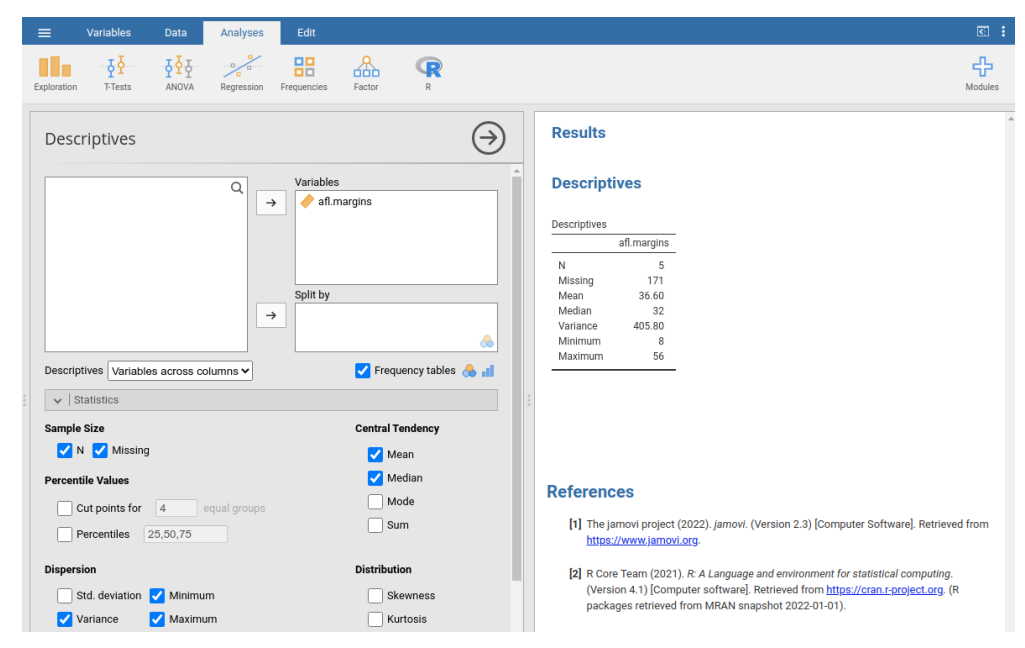
\includegraphics[width=0.9\linewidth]{images/Figure16} \caption{A screenshot of jamovi showing the Variance for the first 5 values of the afl.margins variable}\label{fig:fig4-9}
\end{figure}

As it happens, the answer is no.\footnote{With the possible exception of the third question.} It's not a typo, and jamovi is not making a mistake. In fact, it's very simple to explain what jamovi is doing here, but slightly trickier to explain why jamovi is doing it. So let's start with the ``what''. What jamovi is doing is evaluating a slightly different formula to the one I showed you above. Instead of averaging the squared deviations, which requires you to divide by the number of data points N, jamovi has chosen to divide by \(N - 1\).

{{[}Option: statistical formulae{]}}\footnote{{In other words, the formula that jamovi is using is this one: \[\frac{1}{N-1} \sum_{i=1}^{N} ( X_i - \bar{X} )^2\]}}

So that's the \emph{what}. The real question is why jamovi is dividing by \(N - 1\) and not by \(N\). After all, the variance is supposed to be the mean squared deviation, right? So shouldn't we be dividing by N, the actual number of observations in the sample? Well, yes, we should. However, as we'll discuss in the chapter on {[}Estimating unknown quantities from a sample{]}, there's a subtle distinction between ``describing a sample'' and ``making guesses about the population from which the sample came''. Up to this point, it's been a distinction without a difference. Regardless of whether you're describing a sample or drawing inferences about the population, the mean is calculated exactly the same way. Not so for the variance, or the standard deviation, or for many other measures besides. What I outlined to you initially (i.e., take the actual average, and thus divide by \(N\)) assumes that you literally intend to calculate the variance of the sample. Most of the time, however, you're not terribly interested in the sample in and of itself. Rather, the sample exists to tell you something about the world. If so, you're actually starting to move away from calculating a ``sample statistic'' and towards the idea of estimating a ``population parameter''. However, I'm getting ahead of myself. For now, let's just take it on faith that jamovi knows what it's doing, and we'll revisit the question later on when we talk about estimation in the chapter on {[}Estimating unknown quantities from a sample{]}.

Okay, one last thing. This section so far has read a bit like a mystery novel. I've shown you how to calculate the variance, described the weird ``\(N - 1\)'' thing that jamovi does and hinted at the reason why it's there, but I haven't mentioned the single most important thing. How do you interpret the variance? Descriptive statistics are supposed to describe things, after all, and right now the variance is really just a gibberish number. Unfortunately, the reason why I haven't given you the human-friendly interpretation of the variance is that there really isn't one. This is the most serious problem with the variance. Although it has some elegant mathematical properties that suggest that it really is a fundamental quantity for expressing variation, it's completely useless if you want to communicate with an actual human. Variances are completely uninterpretable in terms of the original variable! All the numbers have been squared and they don't mean anything anymore. This is a huge issue. For instance, according to Table \ref{tab:tab4-3}, the margin in game 1 was ``376.36 points-squared higher than the average margin''. This is \emph{exactly} as stupid as it sounds, and so when we calculate a variance of \(324.64\) we're in the same situation. I've watched a lot of footy games, and at no time has anyone ever referred to ``points squared''. It's not a real unit of measurement, and since the variance is expressed in terms of this gibberish unit, it is totally meaningless to a human.

\hypertarget{standard-deviation}{%
\subsection{Standard deviation}\label{standard-deviation}}

Okay, suppose that you like the idea of using the variance because of those nice mathematical properties that I haven't talked about, but since you're a human and not a robot you'd like to have a measure that is expressed in the same units as the data itself (i.e., points, not points squared). What should you do? The solution to the problem is obvious! Take the square root of the variance, known as the \textbf{standard deviation}, also called the ``root mean squared deviation'', or RMSD. This solves our problem fairly neatly. Whilst nobody has a clue what ``a variance of 324.68 points-squared'' really means, it's much easier to understand ``a standard deviation of 18.01 points'' since it's expressed in the original units. It is traditional to refer to the standard deviation of a sample of data as s, though ``sd'' and ``std dev.'' are also used at times.

{{[}Option: statistical formulae{]}}\footnote{{Because the standard deviation is equal to the square root of the variance, you probably won't be surprised to see that the formula is: \[s=\sqrt{\frac{1}{N} \sum_{i=1}^{N} ( X_i - \bar{X} )^2 }\] and in jamovi there is a check box for `Std. deviation' right above the check box for `Variance'. Selecting this gives a value of \(26.07\) for the standard deviation.}}

However, as you might have guessed from our discussion of the variance, what jamovi actually calculates is slightly different to the formula given above. Just like the we saw with the variance, what jamovi calculates is a version that divides by \(N - 1\) rather than \(N\).

{{[}Option: statistical formulae{]}}\footnote{{For reasons that will make sense when we return to this topic in the chapter on {[}Estimating unknown quantities from a sample{]} I'll refer to this new quantity as \(\hat{\sigma}\) (read as: ``sigma hat''), and the formula for this is: \[\hat{\sigma}=\sqrt{\frac{1}{N-1} \sum_{i=1}^{N} ( X_i - \bar{X} )^2}\]}}

Interpreting standard deviations is slightly more complex. Because the standard deviation is derived from the variance, and the variance is a quantity that has little to no meaning that makes sense to us humans, the standard deviation doesn't have a simple interpretation. As a consequence, most of us just rely on a simple rule of thumb. In general, you should expect 68\% of the data to fall within 1 standard deviation of the mean, 95\% of the data to fall within 2 standard deviation of the mean, and 99.7\% of the data to fall within 3 standard deviations of the mean. This rule tends to work pretty well most of the time, but it's not exact. It's actually calculated based on an assumption that the histogram is symmetric and ``bell shaped''.{[}\^{}04.5{]} As you can tell from looking at the AFL winning margins histogram in Figure \ref{fig:fig4-2}, this isn't exactly true of our data! Even so, the rule is approximately correct. As it turns out, 65.3\% of the AFL margins data fall within one standard deviation of the mean. This is shown visually in \ref{fig:fig4-10}.

\hypertarget{which-measure-to-use}{%
\subsection{Which measure to use?}\label{which-measure-to-use}}

We've discussed quite a few measures of spread: range, IQR, mean absolute deviation, variance and standard deviation; and hinted at their strengths and weaknesses. Here's a quick summary:

\begin{itemize}
\tightlist
\item
  \emph{Range}. Gives you the full spread of the data. It's very vulnerable to outliers and as a consequence it isn't often used unless you have good reasons to care about the extremes in the data.
\item
  \emph{Interquartile range}. Tells you where the ``middle half'' of the data sits. It's pretty robust and complements the median nicely. This is used a lot.
\item
  \emph{Mean absolute deviation}. Tells you how far ``on average'' the observations are from the mean. It's very interpretable but has a few minor issues (not discussed here) that make it less attractive to statisticians than the standard deviation. Used sometimes, but not often.
\item
  \emph{Variance}. Tells you the average squared deviation from the mean. It's mathematically elegant and is probably the ``right'' way to describe variation around the mean, but it's completely uninterpretable because it doesn't use the same units as the data. Almost never used except as a mathematical tool, but it's buried ``under the hood'' of a very large number of statistical tools.
\item
  \emph{Standard deviation}. This is the square root of the variance. It's fairly elegant mathematically and it's expressed in the same units as the data so it can be interpreted pretty well. In situations where the mean is the measure of central tendency, this is the default. This is by far the most popular measure of variation.
\end{itemize}

In short, the IQR and the standard deviation are easily the two most common measures used to report the variability of the data. But there are situations in which the others are used. I've described all of them in this book because there's a fair chance you'll run into most of these somewhere.

\textbackslash begin\{figure\}
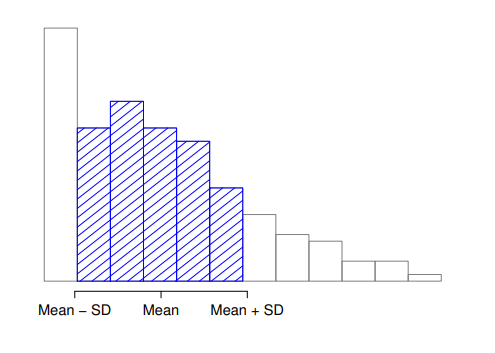
\includegraphics[width=0.9\linewidth]{images/Figure17} \textbackslash caption\{An illustration of the standard deviation from the AFL winning margins data. The shaded bars in the histogram show how much of the data fall within one standard deviation of the mean. In this case, 65.3\% of the data set lies within this range, which is pretty consistent with the `approximately 68\% rule' discussed in the main text\}\label{fig:fig4-10}
\textbackslash end\{figure\}

\hypertarget{skew-and-kurtosis}{%
\section{Skew and kurtosis}\label{skew-and-kurtosis}}

There are two more descriptive statistics that you will sometimes see reported in the psychological literature: skew and kurtosis. In practice, neither one is used anywhere near as frequently as the measures of central tendency and variability that we've been talking about. Skew is pretty important, so you do see it mentioned a fair bit, but I've actually never seen kurtosis reported in a scientific article to date.

\begin{figure}
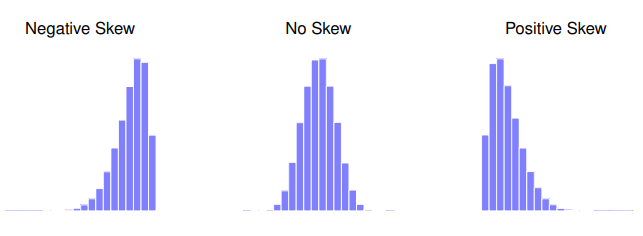
\includegraphics[width=0.9\linewidth]{images/Figure18} \caption{An illustration of skewness. On the left we have a negatively skewed data set ($skewness = -.93$), in the middle we have a data set with no skew (well, hardly any: $skewness = -.006$), and on the right we have a positively skewed data set ($skewness = .93$)}\label{fig:fig4-11}
\end{figure}

Since it's the more interesting of the two, let's start by talking about the \textbf{skewness}. Skewness is basically a measure of asymmetry and the easiest way to explain it is by drawing some pictures. As Figure \ref{fig:fig4-11} illustrates, if the data tend to have a lot of extreme small values (i.e., the lower tail is ``longer'' than the upper tail) and not so many extremely large values (left panel) then we say that the data are \emph{negatively skewed}. On the other hand, if there are more extremely large values than extremely small ones (right panel) we say that the data are positively skewed. That's the qualitative idea behind skewness. If there are relatively more values that are far greater than the mean, the distribution is positively skewed or right skewed, with a tail stretching to the right. Negative or left skew is the opposite. A symmetric distribution has a skewness of 0. The skewness value for a positively skewed distribution is positive, and a negative value for a negatively skewed distribution.

{{[}Option: statistical formulae{]}}\footnote{{One formula for the skewness of a data set is as follows \[    skewness(X)=\frac{1}{N \hat{\sigma}^3} \sum_{i=1}^{N} ( X_i - \bar{X})^3\] where N is the number of observations, \(\bar{X}\) is the sample mean, and \(\hat{\sigma}\) is the standard deviation (the ``divide by \(N - 1\)'' version, that is).}}

Perhaps more helpfully, you can use jamovi to calculate skewness: it's a check box in the `Statistics' options under `Exploration' - `Descriptives'. For the afl.margins variable, the skewness figure is \(0.780\). If you divide the skewness estimate by the Std. error for skewness you have an indication of how skewed the data is. Especially in small samples (N \(<\) 50), one rule of thumb suggests that a value of 2 or less can mean that the data is not very skewed, and a value of over 2 that there is sufficient skew in the data to possibly limit its use in some statistical analyses. Though there is no clear agreement on this interpretation. That said, this does indicate that the AFL winning margins data is somewhat skewed (\(\frac{0.780}{0.183} = 4.262\)).

The final measure that is sometimes referred to, though very rarely in practice, is the kurtosis of a data set. Put simply, kurtosis is a measure of how thin or fat the tails of a distribution are, as illustrated in Figure @ref(fig:fig4.12). By convention, we say that the ``normal curve'' (black lines) has zero kurtosis, so the degree of kurtosis is assessed relative to this curve.

\begin{figure}
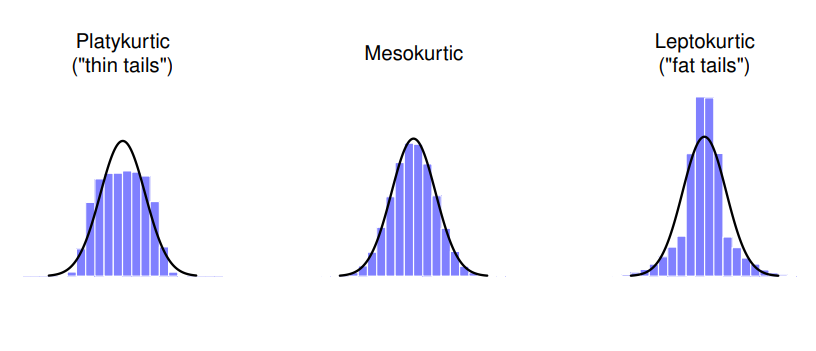
\includegraphics[width=0.9\linewidth]{images/Figure19} \caption{An illustration of kurtosis. On the left, we have a 'platykurtic' distribution (kurtosis = -.95) meaning that the distribution has 'thin' or flat tails. In the middle we have a 'mesokurtic' distribution (kurtosis is almost exactly 0) which means that the tails are neither thin or fat. Finally, on the right, we have a 'leptokurtic' distribution (kurtosis = 2.12) indicating that the distribution has 'fat' tails. Note that kurtosis is measured with respect to a normal curve (black line)}\label{fig:fig4-12}
\end{figure}

In this Figure, the data on the left have a pretty flat distribution, with thin tails, so the kurtosis is negative and we call the data platykurtic. The data on the right have a distribution with fat tails, so the kurtosis is positive and we say that the data is leptokurtic. But the data in the middle have neither think or fat tails, so we say that it is mesokurtic and has kurtosis zero. This is summarised in the table below:

 
  \providecommand{\huxb}[2]{\arrayrulecolor[RGB]{#1}\global\arrayrulewidth=#2pt}
  \providecommand{\huxvb}[2]{\color[RGB]{#1}\vrule width #2pt}
  \providecommand{\huxtpad}[1]{\rule{0pt}{#1}}
  \providecommand{\huxbpad}[1]{\rule[-#1]{0pt}{#1}}

\begin{table}[ht]
\begin{centerbox}
\begin{threeparttable}
\setlength{\tabcolsep}{0pt}
\begin{tabular}{l l l}


\hhline{>{\huxb{0, 0, 0}{0.4}}->{\huxb{0, 0, 0}{0.4}}->{\huxb{0, 0, 0}{0.4}}-}
\arrayrulecolor{black}

\multicolumn{1}{!{\huxvb{0, 0, 0}{0}}c!{\huxvb{0, 0, 0}{0}}}{\cellcolor[RGB]{242, 242, 242}\huxtpad{6pt + 1em}\centering \hspace{0pt} \textbf{English} \hspace{6pt}\huxbpad{6pt}} &
\multicolumn{1}{c!{\huxvb{0, 0, 0}{0}}}{\cellcolor[RGB]{242, 242, 242}\huxtpad{6pt + 1em}\centering \hspace{6pt} \textbf{informal term} \hspace{6pt}\huxbpad{6pt}} &
\multicolumn{1}{c!{\huxvb{0, 0, 0}{0}}}{\cellcolor[RGB]{242, 242, 242}\huxtpad{6pt + 1em}\centering \hspace{6pt} \textbf{kurtosis value} \hspace{0pt}\huxbpad{6pt}} \tabularnewline[-0.5pt]


\hhline{>{\huxb{0, 0, 0}{0.4}}->{\huxb{0, 0, 0}{0.4}}->{\huxb{0, 0, 0}{0.4}}-}
\arrayrulecolor{black}

\multicolumn{1}{!{\huxvb{0, 0, 0}{0}}c!{\huxvb{0, 0, 0}{0}}}{\huxtpad{6pt + 1em}\centering \hspace{0pt} "tails too thin” \hspace{6pt}\huxbpad{6pt}} &
\multicolumn{1}{c!{\huxvb{0, 0, 0}{0}}}{\huxtpad{6pt + 1em}\centering \hspace{6pt} platykurtic \hspace{6pt}\huxbpad{6pt}} &
\multicolumn{1}{c!{\huxvb{0, 0, 0}{0}}}{\huxtpad{6pt + 1em}\centering \hspace{6pt} negative \hspace{0pt}\huxbpad{6pt}} \tabularnewline[-0.5pt]


\hhline{}
\arrayrulecolor{black}

\multicolumn{1}{!{\huxvb{0, 0, 0}{0}}c!{\huxvb{0, 0, 0}{0}}}{\cellcolor[RGB]{242, 242, 242}\huxtpad{6pt + 1em}\centering \hspace{0pt} "tails neither thin or fat" \hspace{6pt}\huxbpad{6pt}} &
\multicolumn{1}{c!{\huxvb{0, 0, 0}{0}}}{\cellcolor[RGB]{242, 242, 242}\huxtpad{6pt + 1em}\centering \hspace{6pt} mesokurtic \hspace{6pt}\huxbpad{6pt}} &
\multicolumn{1}{c!{\huxvb{0, 0, 0}{0}}}{\cellcolor[RGB]{242, 242, 242}\huxtpad{6pt + 1em}\centering \hspace{6pt} zero \hspace{0pt}\huxbpad{6pt}} \tabularnewline[-0.5pt]


\hhline{}
\arrayrulecolor{black}

\multicolumn{1}{!{\huxvb{0, 0, 0}{0}}c!{\huxvb{0, 0, 0}{0}}}{\huxtpad{6pt + 1em}\centering \hspace{0pt} "tails too fat” \hspace{6pt}\huxbpad{6pt}} &
\multicolumn{1}{c!{\huxvb{0, 0, 0}{0}}}{\huxtpad{6pt + 1em}\centering \hspace{6pt} leptokurtic \hspace{6pt}\huxbpad{6pt}} &
\multicolumn{1}{c!{\huxvb{0, 0, 0}{0}}}{\huxtpad{6pt + 1em}\centering \hspace{6pt} positive \hspace{0pt}\huxbpad{6pt}} \tabularnewline[-0.5pt]


\hhline{>{\huxb{0, 0, 0}{0.4}}->{\huxb{0, 0, 0}{0.4}}->{\huxb{0, 0, 0}{0.4}}-}
\arrayrulecolor{black}
\end{tabular}\captionsetup{justification=raggedright,singlelinecheck=off}
\caption{\label{tab:tab4-4} Thin to fat tails to illustrate kurtosis}
 
\end{threeparttable}\par\end{centerbox}

\end{table}
 

{{[}Option: statistical formulae{]}}\footnote{{The equation for kurtosis is pretty similar in spirit to the formulas we've seen already for the variance and the skewness. Except that where the variance involved squared deviations and the skewness involved cubed deviations, the kurtosis involves raising the deviations to the fourth power:\(^b\) \[kurtosis(X)=\frac{1}{N \hat{\sigma}^4} \sum_{i=1}^{N} ( X_i - \bar{X} )^4 - 3\] I know, it's not terribly interesting to me either. --- \(^b\) The ``-3'' part is something that statisticians tack on to ensure that the normal curve has kurtosis zero. It looks a bit stupid, just sticking a ``-3'' at the end of the formula, but there are good mathematical reasons for doing this.}}

More to the point, jamovi has a check box for kurtosis just below the check box for skewness, and this gives a value for kurtosis of \(0.101\) with a standard error of \(0.364\). This means that the AFL winning margins data has only a small kurtosis, which is ok.

\hypertarget{descriptive-statistics-separately-for-each-group}{%
\section{Descriptive statistics separately for each group}\label{descriptive-statistics-separately-for-each-group}}

It is very commonly the case that you find yourself needing to look at descriptive statistics broken down by some grouping variable. This is pretty easy to do in jamovi. For instance, let's say I want to look at the descriptive statistics for some clinical trial data, broken down separately by therapy type. This is a new data set, one that you've never seen before. The data is stored in the clinicaltrial.csv file and we'll use it a lot later on in the chapter on {[}Comparing several means (one-way ANOVA){]} (you can find a complete description of the data at the start of that chapter). Let's load it and see what we've got:

Evidently there were three drugs: a placebo, something called ``anxifree'' and something called ``joyzepam'', and there were 6 people administered each drug. There were 9 people treated using cognitive behavioural therapy (CBT) and 9 people who received no psychological treatment. And we can see from looking at the `Descriptives' of the mood.gain variable that most people did show a mood gain (\(mean = 0.88\)), though without knowing what the scale is here it's hard to say much more than that. Still, that's not too bad. Overall I feel that I learned something from that.

We can also go ahead and look at some other descriptive statistics, and this time separately for each type of therapy. In jamovi, check Std. deviation, Skewness and Kurtosis in the `Statistics' options. At the same time, transfer the therapy variable into the `Split by' box, and you should get something like Figure \ref{fig:fig4-14}

\begin{figure}
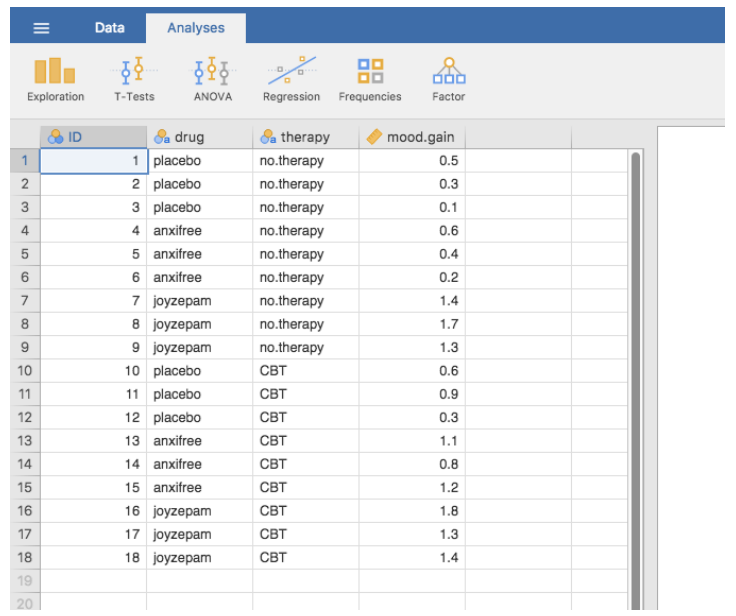
\includegraphics[width=0.9\linewidth]{images/Figure20} \caption{A screenshot of jamovi showing the variables stored in the clinicaltrial.csv file}\label{fig:fig4-13}
\end{figure}

What if you have multiple grouping variables? Suppose you want to look at the average mood gain separately for all possible combinations of drug and therapy. It is possible to do this by adding another variable, drug, into the `Split by' box. Easy peasy, though sometimes if you split too much there isn't enough data in each breakdown combination to make meaningful calculations. In this case jamovi tells you this by stating something like NaN or Inf. \footnote{Sometimes jamovi will also present numbers in an unusual way. If a number is very small, or very large, then jamovi switches to an exponential form for numbers. For example 6.51e-4 is the same as saying that the decimal point is moved 4 places to the left, so the actual number is 0.000651. If there is a plus sign (i.e.~6.51e+4 then the decimal point is moved to the right, i.e.~65,100.00. Usually only very small or very large numbers are expressed in this way, for example 6.51e-16, which would be quite unwieldy to write out in the normal way.}

\begin{figure}
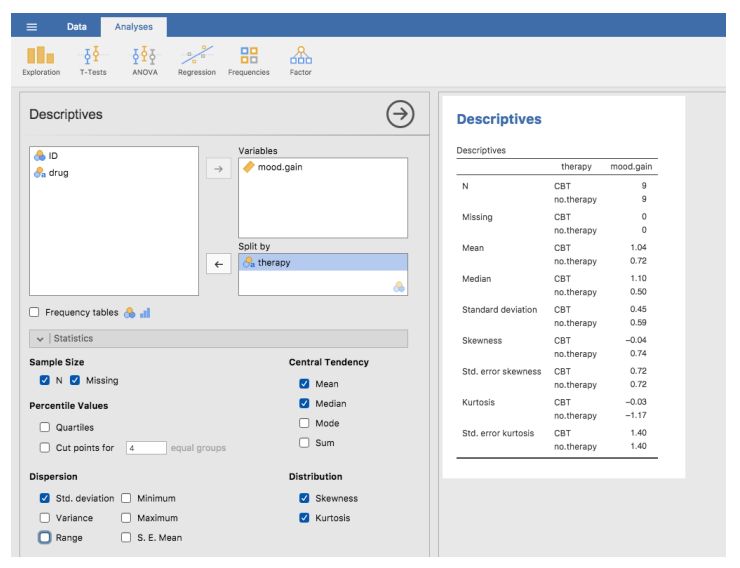
\includegraphics[width=0.9\linewidth]{images/Figure21} \caption{A screenshot of jamovi showing Descriptives split by therapy type}\label{fig:fig4-14}
\end{figure}

\hypertarget{standard-scores}{%
\section{Standard scores}\label{standard-scores}}

Suppose my friend is putting together a new questionnaire intended to measure ``grumpiness''. The survey has \(50\) questions which you can answer in a grumpy way or not. Across a big sample (hypothetically, let's imagine a million people or so!) the data are fairly normally distributed, with the mean grumpiness score being \(17\) out of \(50\) questions answered in a grumpy way, and the standard deviation is \(5\). In contrast, when I take the questionnaire I answer \(35\) out of \(50\) questions in a grumpy way. So, how grumpy am I? One way to think about it would be to say that I have grumpiness of \(\frac{35}{50}\), so you might say that I'm 70\% grumpy. But that's a bit weird, when you think about it. If my friend had phrased her questions a bit differently people might have answered them in a different way, so the overall distribution of answers could easily move up or down depending on the precise way in which the questions were asked. So, I'm only 70\% grumpy \emph{with respect to this set of survey questions}. Even if it's a very good questionnaire this isn't very a informative statement.

A simpler way around this is to describe my grumpiness by comparing me to other people. Shockingly, out of my friend's sample of \(1,000,000\) people, only \(159\) people were as grumpy as me (that's not at all unrealistic, frankly) suggesting that I'm in the top 0.016\% of people for grumpiness. This makes much more sense than trying to interpret the raw data. This idea, that we should describe my grumpiness in terms of the overall distribution of the grumpiness of humans, is the qualitative idea that standardisation attempts to get at. One way to do this is to do exactly what I just did and describe everything in terms of percentiles. However, the problem with doing this is that ``it's lonely at the top''. Suppose that my friend had only collected a sample of \(1000\) people (still a pretty big sample for the purposes of testing a new questionnaire, I'd like to add), and this time gotten, let's say, a mean of \(16\) out of \(50\) with a standard deviation of \(5\). The problem is that almost certainly not a single person in that sample would be as grumpy as me.

However, all is not lost. A different approach is to convert my grumpiness score into a \textbf{standard score}, also referred to as a z-score. The standard score is defined as the number of standard deviations above the mean that my grumpiness score lies. To phrase it in ``pseudomaths'' the standard score is calculated like this:

\[
\text{standard score} = \frac{\text{raw score} - mean}{\text{standard deviation}}
\]

{{[}Option: statistical formulae{]}}\footnote{{In actual maths, the equation for the z-score is \[z_i =\frac{X_i - \bar{X}}{\hat{\sigma}}\]}}

So, going back to the grumpiness data, we can now transform Dani's raw grumpiness into a standardised grumpiness score.

\[ z =\frac{35 - 17}{5} = 3.6 \] To interpret this value, recall the rough heuristic that I provided in the section on \protect\hyperlink{standard-deviation}{Standard deviation} in which I noted that 99.7\% of values are expected to lie within 3 standard deviations of the mean. So the fact that my grumpiness corresponds to a z score of 3.6 indicates that I'm very grumpy indeed. In fact this suggests that I'm grumpier than 99.98\% of people. Sounds about right.

In addition to allowing you to interpret a raw score in relation to a larger population (and thereby allowing you to make sense of variables that lie on arbitrary scales), standard scores serve a second useful function. Standard scores can be compared to one another in situations where the raw scores can't. Suppose, for instance, my friend also had another questionnaire that measured extraversion using a \(24\) item questionnaire. The overall mean for this measure turns out to be 13 with standard deviation \(4\), and I scored a \(2\). As you can imagine, it doesn't make a lot of sense to try to compare my raw score of \(2\) on the extraversion questionnaire to my raw score of 35 on the grumpiness questionnaire. The raw scores for the two variables are ``about'' fundamentally different things, so this would be like comparing apples to oranges.

What about the standard scores? Well, this is a little different. If we calculate the standard scores we get \((z = \frac{(35-17)}{5}=3.6)\) for grumpiness and \((z = \frac{(2-13)}{4}=-2.75)\) for extraversion. These two numbers can be compared to each other.\footnote{Though some caution is usually warranted. It's not always the case that one standard deviation on variable A corresponds to the same ``kind'' of thing as one standard deviation on variable B. Use common sense when trying to determine whether or not the z scores of two variables can be meaningfully compared} I'm much less extraverted than most people (\(z = -2.75\)) and much grumpier than most people (\(z=3.6\)). But the extent of my unusualness is much more extreme for grumpiness, since \(3.6\) is a bigger number than \(2.75\). Because each standardised score is a statement about where an observation falls relative to its own population, it is possible to compare standardised scores across completely different variables.

\hypertarget{summary-2}{%
\section{Summary}\label{summary-2}}

Calculating some basic descriptive statistics is one of the very first things you do when analysing real data, and descriptive statistics are much simpler to understand than inferential statistics, so like every other statistics textbook I've started with descriptives. In this chapter, we talked about the following topics:

\begin{itemize}
\tightlist
\item
  \protect\hyperlink{measures-of-central-tendency}{Measures of central tendency}. Broadly speaking, central tendency measures tell you where the data are. There's three measures that are typically reported in the literature: the mean, median and mode.
\item
  \protect\hyperlink{measures-of-variability}{Measures of variability}. In contrast, measures of variability tell you about how ``spread out'' the data are. The key measures are: range, standard deviation, and interquartile range.
\item
  \protect\hyperlink{skew-and-kurtosis}{Skew and kurtosis}. We also looked at assymetry in a variable's distribution (skew) and thin or fat tailed distributions (kurtosis).
\item
  \protect\hyperlink{descriptive-statistics-separately-for-each-group}{Descriptive statistics separately for each group}. Since this book focuses on doing data analysis in jamovi, we spent a bit of time talking about how descriptive statistics are computed for different subgroups.
\item
  \protect\hyperlink{standard-scores}{Standard scores}. The z-score is a slightly unusual beast. It's not quite a descriptive statistic, and not quite an inference. Make sure you understand this section. It'll come up again later.
\end{itemize}

In the next Chapter we'll move on to a discussion of how to draw pictures! Everyone loves a pretty picture, right? But before we do, I want to end on an important point. A traditional first course in statistics spends only a small proportion of the class on descriptive statistics, maybe one or two lectures at most. The vast majority of the lecturer's time is spent on inferential statistics because that's where all the hard stuff is. That makes sense, but it hides the practical everyday importance of choosing good descriptives. With that in mind\ldots{}

\begin{center}\rule{0.5\linewidth}{0.5pt}\end{center}

\hypertarget{drawing-graphs}{%
\chapter{Drawing graphs}\label{drawing-graphs}}

\begin{quote}
\emph{Above all else show the data.}\\
- Edward Tufte\footnote{The origin of this quote is Tufte's lovely book \emph{The Visual
  Display of Quantitative Information.}}
\end{quote}

Visualising data is one of the most important tasks facing the data
analyst. It's important for two distinct but closely related reasons.
Firstly, there's the matter of drawing ``presentation graphics'',
displaying your data in a clean, visually appealing fashion makes it
easier for your reader to understand what you're trying to tell them.
Equally important, perhaps even more important, is the fact that drawing
graphs helps you to understand the data. To that end, it's important to
draw ``exploratory graphics'' that help you learn about the data as you go
about analysing it. These points might seem pretty obvious but I cannot
count the number of times I've seen people forget them.

To give a sense of the importance of this chapter, I want to start with
a classic illustration of just how powerful a good graph can be. To that
end, Figure \ref{fig:fig5-1} shows a redrawing of one of the most famous data
visualisations of all time. This is John Snow's 1854 map of cholera
deaths. The map is elegant in its simplicity. In the background we have
a street map which helps orient the viewer. Over the top we see a large
number of small dots, each one representing the location of a cholera
case. The larger symbols show the location of water pumps, labelled by
name. Even the most casual inspection of the graph makes it very clear
that the source of the outbreak is almost certainly the Broad Street
pump. Upon viewing this graph Dr Snow arranged to have the handle
removed from the pump and ended the outbreak that had killed over 500
people. Such is the power of a good data visualisation.

The goals in this chapter are twofold. First, to discuss several fairly
standard graphs that we use a lot when analysing and presenting data,
and second to show you how to create these graphs in jamovi. The graphs
themselves tend to be pretty straightforward, so in one respect this
chapter is pretty simple. Where people usually struggle is learning how
to produce graphs, and especially learning how to produce good graphs.
Fortunately, learning how to draw graphs in jamovi is reasonably simple
as long as you're not too picky about what your graph looks like. What I
mean when I say this is that jamovi has a lot of very good default
graphs, or plots, that most of the time produce a clean, high-quality
graphic. However, on those occasions when you do want to do something
non-standard, or if you need to make highly specific changes to the
figure, then the graphics functionality in jamovi is not yet capable of
supporting advanced work or detail editing.

\begin{figure}
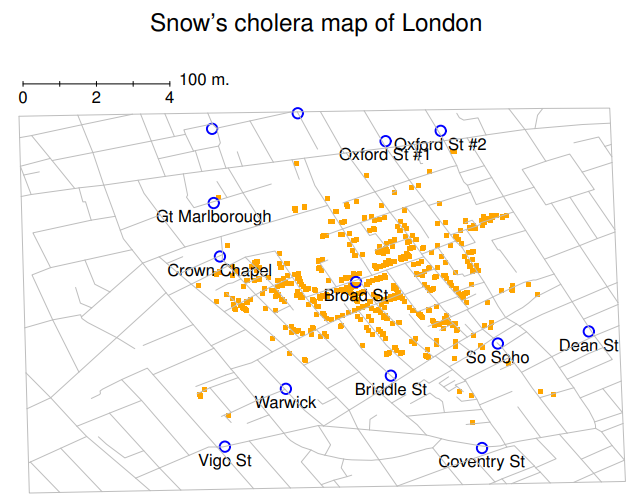
\includegraphics[width=0.9\linewidth]{images/Figure22} \caption{A stylised redrawing of John Snow’s original cholera map. Each small dot represents the location of a cholera case and each large circle shows the location of a well. As the plot makes clear, the cholera outbreak is centred very closely on the Broad St pump}\label{fig:fig5-1}
\end{figure}

\hypertarget{histograms}{%
\section{Histograms}\label{histograms}}

Let's begin with the humble \textbf{histogram}. Histograms are one of the
simplest and most useful ways of visualising data. They make most sense
when you have an interval or ratio scale variable (e.g., the afl.margins
data from the \protect\hyperlink{descriptive-statistics}{Descriptive statistics} chapter and what you want to do is get an overall
impression of the variable. Most of you probably know how histograms
work, since they're so widely used, but for the sake of completeness
I'll describe them. All you do is divide up the possible values into
\textbf{bins} and then count the number of observations that fall within each
bin. This count is referred to as the frequency or density of the bin
and is displayed as a vertical bar. Ihe AFL winning margins data there
are 33 games in which the winning margin was less than 10 points and it
is this fact that is represented by the height of the leftmost bar that
we showed earlier in the \protect\hyperlink{descriptive-statistics}{Descriptive statistics} chapter, Figure \ref{fig:fig4-2}. With these earlier
graphs we used an advanced plotting package in R which, for now, is
beyond the capability of jamovi. But jamovi gets us close, and drawing
this histogram in jamovi is pretty straightforward. Open up the `plots'
options under `Exploration' - `Descriptives' and click the `histogram'
check box, as in Figure \ref{fig:fig5-1}. jamovi defaults to labelling the y-axis
as `density' and the x-axis with the variable name. The \textbf{bins} are
selected automatically, and there is no scale, or count, information on
the y-axis unlike the previous Figure \ref{fig:fig4-2}. But this does not matter
too much because after all what we are really interested in is our
impression of the shape of the distribution: is it normally distributed
or is there a skew or kurtosis? Our first impressions of these
characteristics come from drawing a \textbf{histogram}.

\begin{figure}
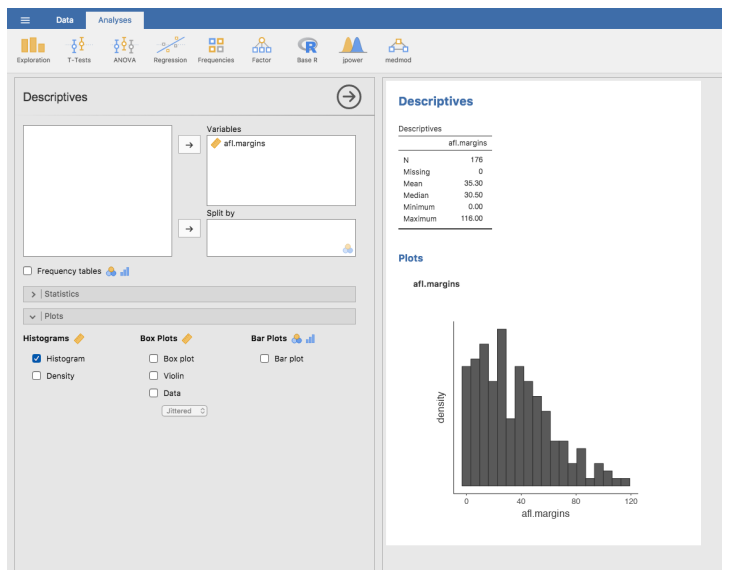
\includegraphics[width=0.9\linewidth]{images/Figure23} \caption{jamovi screen showing the histogram check box}\label{fig:fig5-2}
\end{figure}

One additional feature that jamovi provides is the ability to plot a
`Density' curve. You can do this by clicking the `Density' check box
under the `Plots' options (and unchecking `Histogram'), and this gives
us the plot shown in Figure \ref{fig:fig5-3}. A density plot visualises the
distribution of data over a continuous interval or time period. This
chart is a variation of a histogram that uses \textbf{kernel smoothing} to
plot values, allowing for smoother distributions by smoothing out the
noise. The peaks of a density plot help display where values are
concentrated over the interval. An advantage density plots have over
histograms is that they are better at determining the distribution shape
because they're not affected by the number of bins used (each bar used
in a typical histogram). A histogram comprising of only 4 bins wouldn't
produce a distinguishable enough shape of distribution as a 20-bin
histogram would. However, with density plots, this isn't an issue.

\begin{figure}
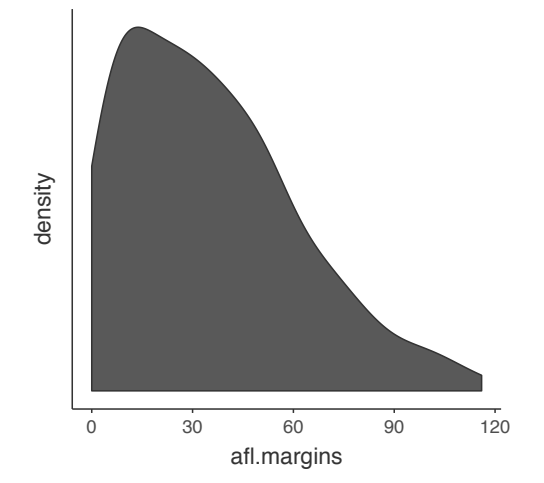
\includegraphics[width=0.9\linewidth]{images/Figure24} \caption{A density plot of the afl.margins variable plotted in jamovi}\label{fig:fig5-3}
\end{figure}

Although this image would need a lot of cleaning up in order to make a
good presentation graphic (i.e., one you'd include in a report), it
nevertheless does a pretty good job of describing the data. In fact, the
big strength of a histogram or density plot is that (properly used) it
does show the entire spread of the data, so you can get a pretty good
sense about what it looks like. The downside to histograms is that they
aren't very compact. Unlike some of the other plots I'll talk about it's
hard to cram 20-30 histograms into a single image without overwhelming
the viewer. And of course, if your data are nominal scale then
histograms are useless.

\hypertarget{boxplots}{%
\section{Boxplots}\label{boxplots}}

Another alternative to histograms is a \textbf{boxplot}, sometimes called a
``box and whiskers'' plot. Like histograms they're most suited to interval
or ratio scale data. The idea behind a boxplot is to provide a simple
visual depiction of the median, the interquartile range, and the range
of the data. And because they do so in a fairly compact way boxplots
have become a very popular statistical graphic, especially during the
exploratory stage of data analysis when you're trying to understand the
data yourself. Let's have a look at how they work, again using the
afl.margins data as our example.

\begin{figure}
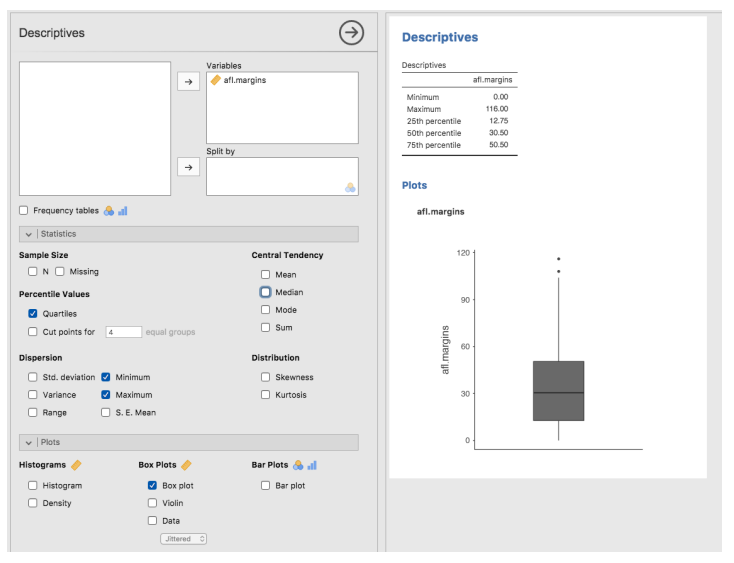
\includegraphics[width=0.9\linewidth]{images/Figure25} \caption{A box plot of the afl.margins variable plotted in jamovi}\label{fig:fig5-4}
\end{figure}

The easiest way to describe what a boxplot looks like is just to draw
one. Click on the `Box plot' check box and you will get the plot shown
on the lower right of Figure \ref{fig:fig5-4}. jamovi has drawn the most basic
boxplot possible. When you look at this plot this is how you should
interpret it: the thick line in the middle of the box is the median; the
box itself spans the range from the 25th percentile to the 75th
percentile; and the ``whiskers'' go out to the most extreme data point
that doesn't exceed a certain bound. By default, this value is 1.5 times
the interquartile range (IQR), calculated as 25th percentile -
(1.5*IQR) for the lower boundary, and 75th percentile + (1.5*IQR) for
the upper boundary. Any observation whose value falls outside this range
is plotted as a circle or dot instead of being covered by the whiskers,
and is commonly referred to as an \textbf{outlier}. For our AFL margins data
there are two observations that fall outside this range, and these
observations are plotted as dots (the upper boundary is 107, and looking
over the data column in the spreadsheet there are two observations with
values higher than this, 108 and 116, so these are the dots).

\hypertarget{violin-plots}{%
\subsection{Violin plots}\label{violin-plots}}

\begin{figure}
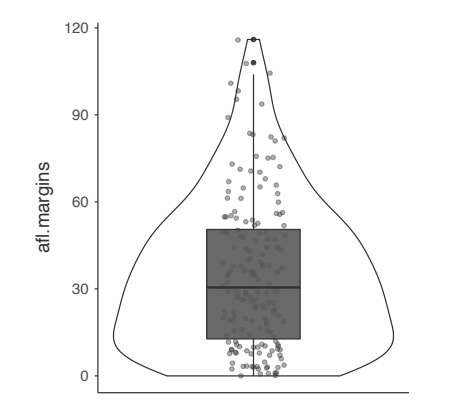
\includegraphics[width=0.9\linewidth]{images/Figure26} \caption{A violin plot of the afl.margins variable plotted in jamovi, also showing a box plot and data points}\label{fig:fig5-5}
\end{figure}

A variation to the traditional box plot is the violin plot. Violin plots
are similar to box plots except that they also show the kernel
probability density of the data at different values. Typically, violin
plots will include a marker for the median of the data and a box
indicating the interquartile range, as in standard box plots. In jamovi
you can achieve this sort of functionality by checking both the `Violin'
and the 'Box plot' check boxes. See Figure \ref{fig:fig5-5}, which also has the
`Data' check box turned on to show the actual data points on the plot.
This does tend to make the graph a bit too busy though, in my opinion.
Clarity is simplicity, so in practice it might be better to just use a
simple box plot.

\hypertarget{drawing-multiple-boxplots}{%
\subsection{Drawing multiple boxplots}\label{drawing-multiple-boxplots}}

One last thing. What if you want to draw multiple boxplots at once?
Suppose, for instance, I wanted separate boxplots showing the AFL
margins not just for 2010 but for every year between 1987 and 2010. To
do that the first thing we'll have to do is find the data. These are
stored in the \textbf{aflmarginbyyear.csv} file. So let's load it into jamovi
and see what is in it. You will see that it is a pretty big data set. It
contains 4296 games and the variables that we're interested in. What we
want to do is have jamovi draw boxplots for the margin variable, but
plotted separately for each year. The way to do this is to move the year
variable across into the `Split by' box, as in Figure \ref{fig:fig5-6}.

\begin{figure}
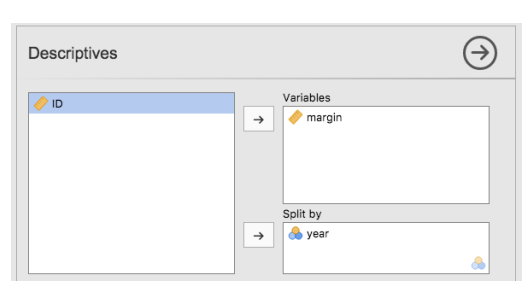
\includegraphics[width=0.9\linewidth]{images/Figure27} \caption{jamovi screen shot showing the ‘Split by’ window}\label{fig:fig5-6}
\end{figure}

The result is shown in Figure \ref{fig:fig5-7}. This version of the box plot,
split by year, gives a sense of why it's sometimes useful to choose box
plots instead of histograms. It's possible to get a good sense of what
the data look like from year to year without getting overwhelmed with
too much detail. Now imagine what would have happened if I'd tried to
cram 24 histograms into this space: no chance at all that the reader is
going to learn anything useful.

\begin{figure}
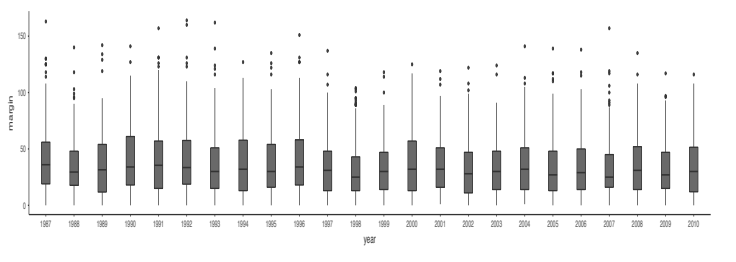
\includegraphics[width=0.9\linewidth]{images/Figure28} \caption{Multiple boxplots plotted in jamovi, for the margin by year variables in the aflsmall2 data set}\label{fig:fig5-7}
\end{figure}

\hypertarget{using-box-plots-to-detect-outliers}{%
\subsection{Using box plots to detect outliers}\label{using-box-plots-to-detect-outliers}}

Because the boxplot automatically separates out those observations that
lie outside a certain range, depicting them with a dot in jamovi, people
often use them as an informal method for detecting \textbf{outliers}:
observations that are ``suspiciously'' distant from the rest of the data.
Here's an example. Suppose that I'd drawn the boxplot for the AFL
margins data and it came up looking like Figure \ref{fig:fig5-8}. It's pretty clear
that something funny is going on with two of the observations.
Apparently, there were two games in which the margin was over 300
points! That doesn't sound right to me. Now that I've become suspicious
it's time to look a bit more closely at the data. In jamovi you can
quickly find out which of these observations are suspicious and then you
can go back to the raw data to see if there has been a mistake in data
entry. To do this you need to set up a filter so that only those
observations with values over a certain threshold are included. In our
example, the threshold is over 300, so that is the filter we will
create. First, click on the `Filters' button at the top of the jamovi
window, and then type `margin \textgreater{} 300' into the filter field, as in
Figure \ref{fig:fig5-9}.

\begin{figure}
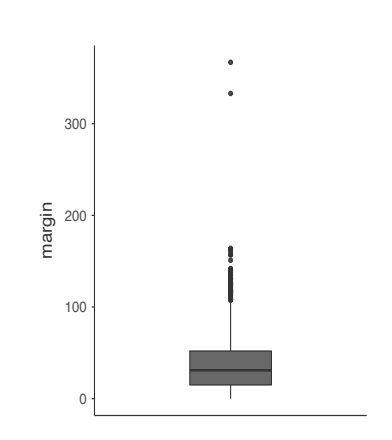
\includegraphics[width=0.9\linewidth]{images/Figure29} \caption{A boxplot showing two very suspicious outliers!}\label{fig:fig5-8}
\end{figure}

This filter creates a new column in the spreadsheet view where only
those observations that pass the filter are included. One neat way to
quickly identify which observations these are is to tell jamovi to
produce a `Frequency table' (in the `Exploration' - `Descriptives'
window) for the ID variable (which must be a nominal variable otherwise
the Frequency table is not produced). In Figure \ref{fig:fig5-10} you can see that
the ID values for the observations where the margin was over 300 are 14
and 134. These are suspicious cases, or observations, where you should
go back to the original data source to find out what is going on.

\begin{figure}
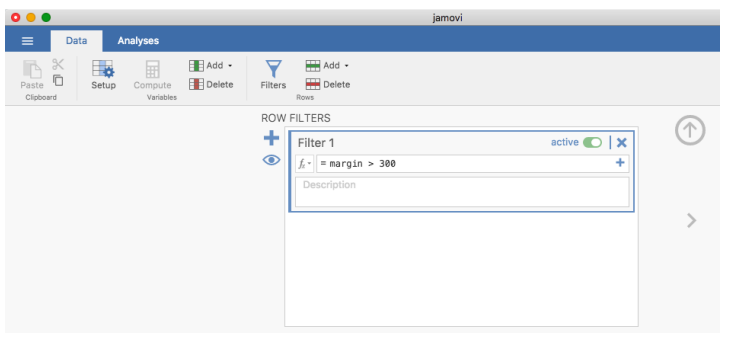
\includegraphics[width=0.9\linewidth]{images/Figure30} \caption{The jamovi filter screen}\label{fig:fig5-9}
\end{figure}

\begin{figure}
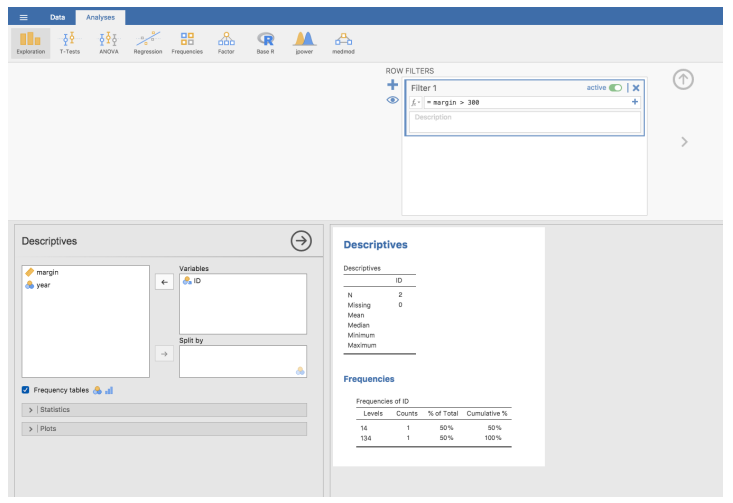
\includegraphics[width=0.9\linewidth]{images/Figure31} \caption{Frequency table for ID showing the ID numbers for the two suspicious outliers: 14 and 134}\label{fig:fig5-10}
\end{figure}

Usually you find that someone has just typed in the wrong number. Whilst
this might seem like a silly example, I should stress that this kind of
thing actually happens a lot. Real world data sets are often riddled
with stupid errors, especially when someone had to type something into a
computer at some point. In fact, there's actually a name for this phase
of data analysis and in practice it can take up a huge chunk of our
time: data cleaning. It involves searching for typing mistakes
(``typos''), missing data and all sorts of other obnoxious errors in raw
data files.

For less extreme values, even if they are flagged in a a boxplot as
outliers, the decision about whether to include outliers or exclude them
in any analysis depends heavily on why you think the data look they way
they do and what you want to use the data for. You really need to
exercise good judgement here. If the outlier looks legitimate to you,
then keep it. In any case, I'll return to the topic again in the section on \protect\hyperlink{model-checking}{Model checking} in the chapter on {[}Correlation and linear regression{]}.

\hypertarget{bar-graphs}{%
\section{Bar graphs}\label{bar-graphs}}

Another form of graph that you often want to plot is the \textbf{bar graph}.
Let's use the afl.finalists data set with the afl.finalists variable
that I introduced in Section 4.1.6. What I want to do is draw a bar
graph that displays the number of finals that each team has played in
over the time spanned by the afl.finalists data set. There are lots of
teams, but I am particularly interested in just four: Brisbane, Carlton,
Fremantle and Richmond. So the first step is to set up a filter so just
those four teams are included in the bar graph. This is straightforward
in jamovi and you can do it by using the `Filters' function that we used
previously. Open up the `Filters' screen and type in the following:

afl.finalists \(==\) `Brisbane' or afl.finalists \(==\) `Carlton' or
afl.finalists \(==\) `Fremantle' or afl.finalists \(==\) `Richmond' \footnote{jamovi uses the symbol ``=='' here to mean ``matches''.}

When you have done this you will see, in the `Data' view, that jamovi
has filtered out all values apart from those we have specified. Next,
open up the `Exploration' - `Descriptives' window and click on the `Bar
plot' check box (remember to move the `afl.finalists' variable across
into the `Variables' box so that jamovi knows which variable to use).
You should then get a bar graph, something like that shown in Figure
\ref{fig:fig5-11}.

\begin{figure}
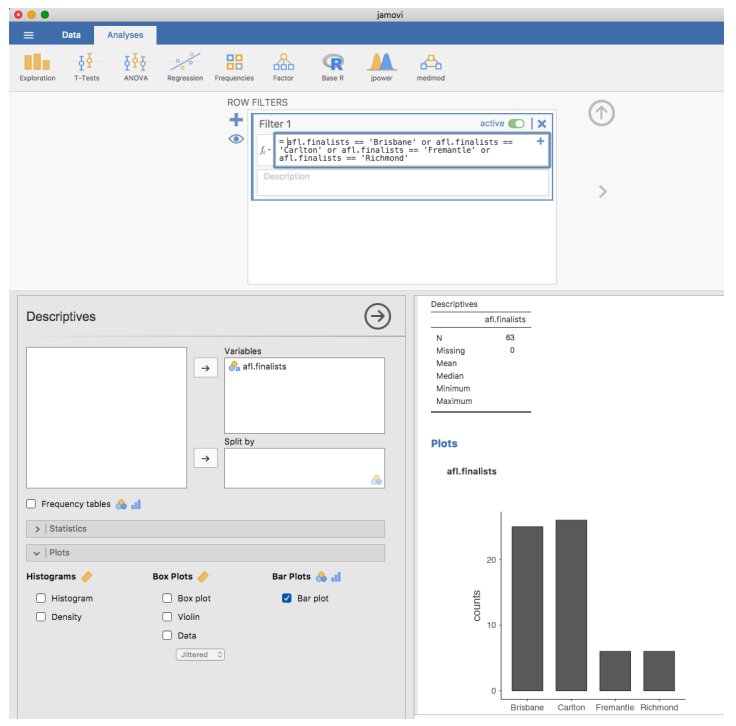
\includegraphics[width=0.9\linewidth]{images/Figure32} \caption{Filtering to include just four AFL teams, and drawing a bar plot in jamovi}\label{fig:fig5-11}
\end{figure}

\hypertarget{saving-image-files-using-jamovi}{%
\section{Saving image files using jamovi}\label{saving-image-files-using-jamovi}}

Hold on, you might be thinking. What's the good of being able to draw
pretty pictures in jamovi if I can't save them and send them to friends
to brag about how awesome my data is? How do I save the picture?
Simples. Just right click on the plot image and export it to a file,
either as `png', `eps', `svg' or `pdf'. These formats all produce nice
images that you can the send to your friends, or include in your
assignments or papers.

\hypertarget{summary-3}{%
\section{Summary}\label{summary-3}}

Perhaps I'm a simple minded person, but I love pictures. Every time I
write a new scientific paper one of the first things I do is sit down
and think about what the pictures will be. In my head an article is
really just a sequence of pictures linked together by a story. All the
rest of it is just window dressing. What I'm really trying to say here
is that the human visual system is a very powerful data analysis tool.
Give it the right kind of information and it will supply a human reader
with a massive amount of knowledge very quickly. Not for nothing do we
have the saying ``a picture is worth a thousand words''. With that in
mind, I think that this is one of the most important chapters in the
book. The topics covered were:

\begin{itemize}
\tightlist
\item
  \emph{Common plots}. Much of the chapter was focused on standard graphs
  that statisticians like to produce: \protect\hyperlink{histograms}{Histograms},
  \protect\hyperlink{boxplots}{Boxplots} and \protect\hyperlink{bar-graphs}{Bar graphs}
\item
  \protect\hyperlink{saving-image-files-using-jamovi}{Saving image files using jamovi}. Importantly, we also covered how to export
  your pictures.
\end{itemize}

One final thing to point out. Whilst jamovi produces some really neat
default graphics, editing the plots is currently not possible. For more
advanced graphics and plotting capability the packages available in R
are much more powerful. One of the most popular graphics systems is
provided by the ggplot2 package (see
https://ggplot2.tidyverse.org/), which is loosely based on ``The
grammar of graphics'' (\protect\hyperlink{ref-Wilkinson2006}{Wilkinson et al. 2006}). It's not for novices. You need to have a pretty good grasp of R before
you can start using it, and even then it takes a while to really get the
hang of it. But when you're ready it's worth taking the time to teach
yourself, because it's a much more powerful and cleaner system.

\begin{center}\rule{0.5\linewidth}{0.5pt}\end{center}

\hypertarget{pragmatic-matters}{%
\chapter{Pragmatic matters}\label{pragmatic-matters}}

\begin{quote}
\emph{The garden of life never seems to confine itself to the plots
philosophers have laid out for its convenience. Maybe a few more
tractors would do the trick.}\\
- Roger Zelazny\footnote{The quote comes from Home is the Hangman, published in 1975.}
\end{quote}

This is a somewhat strange chapter, even by my standards. My goal in
this chapter is to talk a bit more honestly about the realities of
working with data than you'll see anywhere else in the book. The problem
with real world data sets is that they are \emph{messy}. Very often the data
file that you start out with doesn't have the variables stored in the
right format for the analysis you want to do. Sometimes there might be a
lot of missing values in your data set. Sometimes you only want to
analyse a subset of the data. Et cetera. In other words, there's a lot
of \textbf{data manipulation} that you need to do just to get the variables
in your data set into the format that you need it. The purpose of this
chapter is to provide a basic introduction to these pragmatic topics.
Although the chapter is motivated by the kinds of practical issues that
arise when manipulating real data, I'll stick with the practice that
I've adopted through most of the book and rely on very small, toy data
sets that illustrate the underlying issue. Because this chapter is
essentially a collection of techniques and doesn't tell a single
coherent story, it may be useful to start with a list of topics:

\begin{itemize}
\tightlist
\item
  \protect\hyperlink{tabulating-and-cross-tabulating-data}{Tabulating and cross-tabulating data}
\item
  \protect\hyperlink{logical-expressions-in-jamovi}{Logical expressions in jamovi}
\item
  \protect\hyperlink{transforming-and-recoding-a-variable}{Transforming and recoding a variable}
\item
  \protect\hyperlink{a-few-more-mathematical-functions-and-operations}{A few more mathematical functions and operations}
\item
  \protect\hyperlink{extracting-a-subset-of-the-data}{Extracting a subset of the data}
\end{itemize}

As you can see, the list of topics that the chapter covers is pretty broad, and there's a lot of content there. Even though this is one of
the longest and hardest chapters in the book, I'm really only scratching the surface of several fairly different and important topics. My advice, as usual, is to read through the chapter once and try to follow as much of it as you can. Don't worry too much if you can't grasp it all at once, especially the later sections. The rest of the book is only lightly reliant on this chapter so you can get away with just
understanding the basics. However, what you'll probably find is that later on you'll need to flick back to this chapter in order to
understand some of the concepts that I refer to here.

\hypertarget{tabulating-and-cross-tabulating-data}{%
\section{Tabulating and cross-tabulating data}\label{tabulating-and-cross-tabulating-data}}

A very common task when analysing data is the construction of frequency
tables, or crosstabulation of one variable against another. These tasks
can be achieved in jamovi and I'll show you how in this section.

\hypertarget{creating-tables-for-single-variables}{%
\subsection{Creating tables for single variables}\label{creating-tables-for-single-variables}}

Let's start with a simple example. As the father of a small child I
naturally spend a lot of time watching TV shows like In the \emph{Night
Garden}. In the nightgarden.csv file, I've transcribed a short section
of the dialogue. The file contains two variables of interest, speaker
and utterance. Open up this data set in jamovi and take a look at the
data in the `spreadsheet' view. You will see that the data looks
something like this:

`speaker' variable: upsy-daisy upsy-daisy upsy-daisy upsy-daisy
tombliboo tombliboo makka-pakka makka-pakka makka-pakka makka-pakka
`utterance' variable: pip pip onk onk ee oo pip pip onk onk

Looking at this it becomes very clear what happened to my sanity! With
these as my data, one task I might find myself needing to do is
construct a frequency count of the number of words each character speaks
during the show. The jamovi `Descriptives' screen has a check box called
`Frequency tables' which does just this, see Table \ref{tab:tab6-1}.

 
  \providecommand{\huxb}[2]{\arrayrulecolor[RGB]{#1}\global\arrayrulewidth=#2pt}
  \providecommand{\huxvb}[2]{\color[RGB]{#1}\vrule width #2pt}
  \providecommand{\huxtpad}[1]{\rule{0pt}{#1}}
  \providecommand{\huxbpad}[1]{\rule[-#1]{0pt}{#1}}

\begin{table}[ht]
\begin{centerbox}
\begin{threeparttable}
\setlength{\tabcolsep}{0pt}
\begin{tabular}{l l l l}


\hhline{>{\huxb{0, 0, 0}{0.4}}->{\huxb{0, 0, 0}{0.4}}->{\huxb{0, 0, 0}{0.4}}->{\huxb{0, 0, 0}{0.4}}-}
\arrayrulecolor{black}

\multicolumn{1}{!{\huxvb{0, 0, 0}{0}}c!{\huxvb{0, 0, 0}{0}}}{\cellcolor[RGB]{242, 242, 242}\huxtpad{6pt + 1em}\centering \hspace{0pt} \textbf{levels} \hspace{6pt}\huxbpad{6pt}} &
\multicolumn{1}{c!{\huxvb{0, 0, 0}{0}}}{\cellcolor[RGB]{242, 242, 242}\huxtpad{6pt + 1em}\centering \hspace{6pt} \textbf{Counts} \hspace{6pt}\huxbpad{6pt}} &
\multicolumn{1}{c!{\huxvb{0, 0, 0}{0}}}{\cellcolor[RGB]{242, 242, 242}\huxtpad{6pt + 1em}\centering \hspace{6pt} \textbf{\% of Total} \hspace{6pt}\huxbpad{6pt}} &
\multicolumn{1}{c!{\huxvb{0, 0, 0}{0}}}{\cellcolor[RGB]{242, 242, 242}\huxtpad{6pt + 1em}\centering \hspace{6pt} \textbf{Cumulative \%} \hspace{0pt}\huxbpad{6pt}} \tabularnewline[-0.5pt]


\hhline{>{\huxb{0, 0, 0}{0.4}}->{\huxb{0, 0, 0}{0.4}}->{\huxb{0, 0, 0}{0.4}}->{\huxb{0, 0, 0}{0.4}}-}
\arrayrulecolor{black}

\multicolumn{1}{!{\huxvb{0, 0, 0}{0}}c!{\huxvb{0, 0, 0}{0}}}{\huxtpad{6pt + 1em}\centering \hspace{0pt} makka-pakka \hspace{6pt}\huxbpad{6pt}} &
\multicolumn{1}{c!{\huxvb{0, 0, 0}{0}}}{\huxtpad{6pt + 1em}\centering \hspace{6pt} 4 \hspace{6pt}\huxbpad{6pt}} &
\multicolumn{1}{c!{\huxvb{0, 0, 0}{0}}}{\huxtpad{6pt + 1em}\centering \hspace{6pt} 40 \% \hspace{6pt}\huxbpad{6pt}} &
\multicolumn{1}{c!{\huxvb{0, 0, 0}{0}}}{\huxtpad{6pt + 1em}\centering \hspace{6pt} 40 \% \hspace{0pt}\huxbpad{6pt}} \tabularnewline[-0.5pt]


\hhline{}
\arrayrulecolor{black}

\multicolumn{1}{!{\huxvb{0, 0, 0}{0}}c!{\huxvb{0, 0, 0}{0}}}{\cellcolor[RGB]{242, 242, 242}\huxtpad{6pt + 1em}\centering \hspace{0pt} tombliboo \hspace{6pt}\huxbpad{6pt}} &
\multicolumn{1}{c!{\huxvb{0, 0, 0}{0}}}{\cellcolor[RGB]{242, 242, 242}\huxtpad{6pt + 1em}\centering \hspace{6pt} 2 \hspace{6pt}\huxbpad{6pt}} &
\multicolumn{1}{c!{\huxvb{0, 0, 0}{0}}}{\cellcolor[RGB]{242, 242, 242}\huxtpad{6pt + 1em}\centering \hspace{6pt} 20 \% \hspace{6pt}\huxbpad{6pt}} &
\multicolumn{1}{c!{\huxvb{0, 0, 0}{0}}}{\cellcolor[RGB]{242, 242, 242}\huxtpad{6pt + 1em}\centering \hspace{6pt} 60 \% \hspace{0pt}\huxbpad{6pt}} \tabularnewline[-0.5pt]


\hhline{}
\arrayrulecolor{black}

\multicolumn{1}{!{\huxvb{0, 0, 0}{0}}c!{\huxvb{0, 0, 0}{0}}}{\huxtpad{6pt + 1em}\centering \hspace{0pt} upsy-daisy \hspace{6pt}\huxbpad{6pt}} &
\multicolumn{1}{c!{\huxvb{0, 0, 0}{0}}}{\huxtpad{6pt + 1em}\centering \hspace{6pt} 4 \hspace{6pt}\huxbpad{6pt}} &
\multicolumn{1}{c!{\huxvb{0, 0, 0}{0}}}{\huxtpad{6pt + 1em}\centering \hspace{6pt} 40 \% \hspace{6pt}\huxbpad{6pt}} &
\multicolumn{1}{c!{\huxvb{0, 0, 0}{0}}}{\huxtpad{6pt + 1em}\centering \hspace{6pt} 100 \% \hspace{0pt}\huxbpad{6pt}} \tabularnewline[-0.5pt]


\hhline{>{\huxb{0, 0, 0}{0.4}}->{\huxb{0, 0, 0}{0.4}}->{\huxb{0, 0, 0}{0.4}}->{\huxb{0, 0, 0}{0.4}}-}
\arrayrulecolor{black}
\end{tabular}\captionsetup{justification=raggedright,singlelinecheck=off}
\caption{\label{tab:tab6-1} Frequency table for the speaker variable}
 
\end{threeparttable}\par\end{centerbox}

\end{table}
 

The output here tells us on the first line that what we're looking at is
a tabulation of the speaker variable. In the `Levels' column it lists
all the different speakers that exist in the data, and in the `Counts'
column it tells you how many times that speaker appears in the data. In
other words, it's a frequency table.

In jamovi, the `Frequency tables' check box will only produce a table
for single variables. For a table of two variables, for example
combining speaker and utterance so that we can see how many times each
speaker said a particular utterance, we need a cross-tabulation or
contingency table. In jamovi you can do this by selecting the
`Frequencies' - `Contingency Tables' - `Independent Samples' analysis,
and moving the speaker variable into the `Rows' box, and the utterances
variable into the `Columns' box. You then should have a contingency
table like the one shown in Figure \ref{fig:fig6-1}.

\begin{figure}
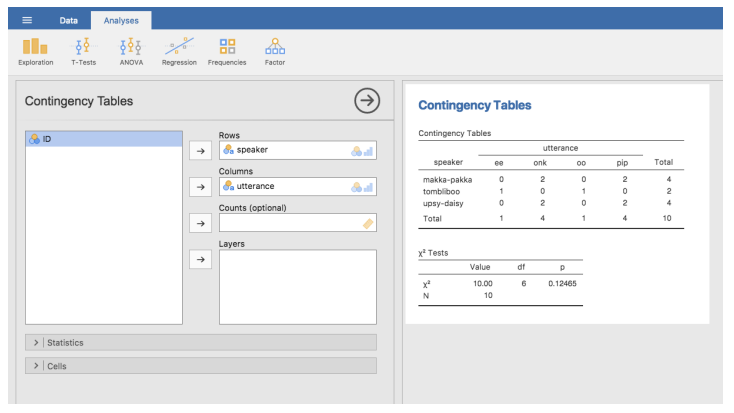
\includegraphics[width=0.9\linewidth]{images/Figure33} \caption{Contingency table for the speaker and utterances variables}\label{fig:fig6-1}
\end{figure}

Don't worry about the ``\(\chi^2\) Tests'' table that is produced. We
are going to cover this later on in the chapter on \protect\hyperlink{categorical-data-analysis}{Categorical data analysis}. When interpreting
the contingency table remember that these are counts, so the fact that
the first row and second column of numbers corresponds to a value of 2
indicates that Makka-Pakka (row 1) says ``onk'' (column 2) twice in this
data set.

\hypertarget{adding-percentages-to-a-contingency-table}{%
\subsection{Adding percentages to a contingency table}\label{adding-percentages-to-a-contingency-table}}

The contingency table shown in Figure \ref{fig:fig6-1} shows a table of raw
frequencies. That is, a count of the total number of cases for different
combinations of levels of the specified variables. However, often you
want your data to be organised in terms of percentages as well as
counts. You can find the check boxes for different percentages under the
`Cells' option in the `Contingency Tables' window. First, click on the
`Row' check box and the Contingency Table in the output window will
change to the one in Figure \ref{fig:fig6-2}.

\begin{figure}
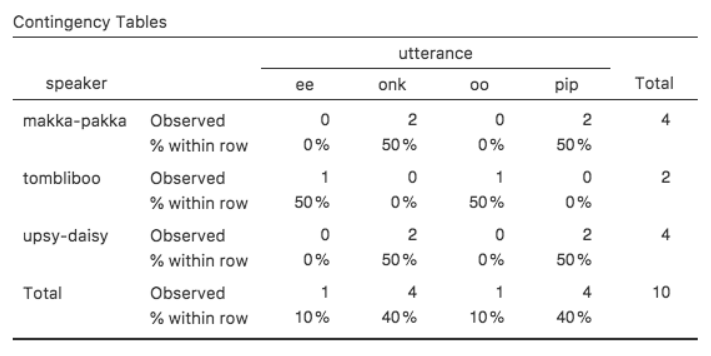
\includegraphics[width=0.9\linewidth]{images/Figure34} \caption{Contingency table for the speaker and utterances variables, with row percentages}\label{fig:fig6-2}
\end{figure}

\begin{figure}
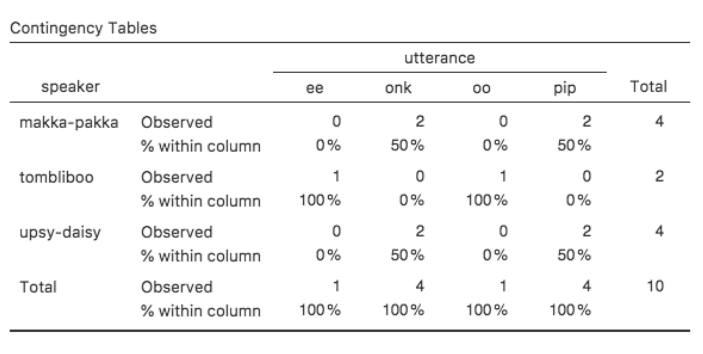
\includegraphics[width=0.9\linewidth]{images/Figure35} \caption{Contingency table for the speaker and utterances variables, with column percentages}\label{fig:fig6-3}
\end{figure}

What we're looking at here is the percentage of utterances made by each
character. In other words, 50\% of Makka-Pakka's utterances are ``pip'',
and the other 50\% are ``onk''. Let's contrast this with the table we get
when we calculate column percentages (uncheck `Row' and check `Column'
in the Cells options window), see Figure \ref{fig:fig6-3}. In this version, what
we're seeing is the percentage of characters associated with each
utterance. For instance, whenever the utterance ``ee'' is made (in this
data set), 100\% of the time it's a Tombliboo saying it.

\hypertarget{logical-expressions-in-jamovi}{%
\section{Logical expressions in jamovi}\label{logical-expressions-in-jamovi}}

A key concept that a lot of data transformations in jamovi rely on is
the idea of a \textbf{logical value}. A logical value is an assertion about
whether something is true or false. This is implemented in jamovi in a
pretty straightforward way. There are two logical values, namely TRUE
and FALSE. Despite the simplicity, logical values are very useful
things. Let's see how they work.

\hypertarget{assessing-mathematical-truths}{%
\subsection{Assessing mathematical truths}\label{assessing-mathematical-truths}}

In George Orwell's classic book 1984 one of the slogans used by the
totalitarian Party was ``two plus two equals five''. The idea being that
the political domination of human freedom becomes complete when it is
possible to subvert even the most basic of truths. It's a terrifying
thought, especially when the protagonist Winston Smith finally breaks
down under torture and agrees to the proposition. ``Man is infinitely
malleable'', the book says. I'm pretty sure that this isn't true of
humans\footnote{I offer up my teenage attempts to be ``cool'' as evidence that some
  things just can't be done.} and it's definitely not true of jamovi. jamovi is
not infinitely malleable, it has rather firm opinions on the topic of
what is and isn't true, at least as regards basic mathematics. If I ask
it to calculate \(2 + 2\)\footnote{You can do this in the Compute new variable screen, though just
  calculating 2 + 2 for every cell of a new variable is not very useful!}, it always gives the same answer,
and it's not bloody 5!

Of course, so far jamovi is just doing the calculations. I haven't asked
it to explicitly assert that \(2 + 2 = 4\) is a true statement. If I want
jamovi to make an explicit judgement, I can use a command like this: \(2 + 2 == 4\)

What I've done here is use the \textbf{equality operator}, \(==\), to force
jamovi to make a ``true or false'' judgement.\footnote{Note that this is a very different operator to the equals operator
  =. A common typo that people make when trying to write logical commands
  in jamovi (or other languages, since the ``= versus =='' distinction is
  important in many computer and statistical programs) is to accidentally
  type = when you really mean ==. Be especially cautious with this, I've
  been programming in various languages since I was a teenager and I still
  screw this up a lot. Hmm. I think I see why I wasn't cool as a teenager.
  And why I'm still not cool.} Okay, let's
see what jamovi thinks of the Party slogan, so type this into the
compute new variable `formula' box:

\[2 + 2 == 5\]

And what do you get? It should be a whole set of `false' values in the
spreadsheet column for your newly computed variable. Booyah! Freedom and
ponies for all! Or something like that. Anyway, it was worth having a
look at what happens if I try to force jamovi to believe that two plus
two is five by making a statement like \(2 + 2 = 5\). I know that if I
do this in another program, say R, then it throws up an error message.
But wait, if you do this in jamovi you get a whole set of `false'
values. So what is going on? Well, it seems that jamovi is being pretty
smart and realises that you are testing whether it is TRUE or FALSE that
\(2 + 2 = 5\), regardless of whether you use the correct \textbf{equality
operator}, \(==\), or the equals sign ``\(=\)''.

Anyway, it was worth having a look at what happens if I try to force
jamovi to believe that two plus two is five by making a statement like
\(2 + 2 = 5\). I know that if I do this in another program, say R,
then it throws up an error message. But wait, if you do this in jamovi
you get a whole set of `false' values. So what is going on? Well, it
seems that jamovi is being pretty smart and realises that you are
testing whether it is TRUE or FALSE that \(2 + 2 = 5\), regardless of
whether you use the correct \textbf{equality operator}, \(==\), or the equals
sign ``\(=\)''.

\hypertarget{logical-operations}{%
\subsection{Logical operations}\label{logical-operations}}

So now we've seen logical operations at work. But so far we've only seen
the simplest possible example. You probably won't be surprised to
discover that we can combine logical operations with other operations
and functions in a more complicated way, like this: \(3 \times 3 + 4 \times 4 == 5 \times 5\)
or this \(SQRT(25) == 5\)

Not only that, but as Table \ref{tab:tab6-2} illustrates, there are several other
logical operators that you can use corresponding to some basic
mathematical concepts. Hopefully these are all pretty self-explanatory.
For example, the \textbf{less than} operator \textless{} checks to see if the number
on the left is less than the number on the right. If it's less, then
jamovi returns an answer of TRUE, but if the two numbers are equal, or
if the one on the right is larger, then jamovi returns an answer of
FALSE.

In contrast, the \textbf{less than or equal to} operator \(<=\) will do exactly
what it says. It returns a value of TRUE if the number of the left hand
side is less than or equal to the number on the right hand side. At this
point I hope it's pretty obvious what the \textbf{greater than} operator \(<\)
and the \textbf{greater than or equal to} operator \(<=\) do!

Next on the list of logical operators is the \textbf{not equal to} operator
!= which, as with all the others, does what it says it does. It returns
a value of TRUE when things on either side are not identical to each
other. Therefore, since \(2 + 2\) isn't equal to \(5\), we would get `true' as
the value for our newly computed variable. Try it and see:

\[2 + 2 \text{ != } 5\]

We're not quite done yet. There are three more logical operations that
are worth knowing about, listed in Table \ref{tab:tab6-3}. These are the \textbf{not}
operator !, the \textbf{and} operator and, and the \textbf{or} operator or. Like
the other logical operators, their behaviour is more or less exactly
what you'd expect given their names. For instance, if I ask you to
assess the claim that ``either \(2 + 2 = 4\) or \(2 + 2 = 5\)'' you'd
say that it's true. Since it's an ``either-or'' statement, all we need is
for one of the two parts to be true. That's what the or operator
does:\footnote{Now, here's a quirk in jamovi. When you have simple logical
  expressions like the ones we have already met, e.g.~2 + 2 == 5 then
  jamovi neatly states `false' (or `true') in the corresponding
  spreadsheet column. Underneath the hood, jamovi stores `false' as 0 and
  `true' as 1. When we have more complex logical expressions, such as (2+2
  == 4) or (2+2 == 5), then jamovi just displays either 0 or 1, depending
  whether the logical expression is evaluated as false, or true.}

 
  \providecommand{\huxb}[2]{\arrayrulecolor[RGB]{#1}\global\arrayrulewidth=#2pt}
  \providecommand{\huxvb}[2]{\color[RGB]{#1}\vrule width #2pt}
  \providecommand{\huxtpad}[1]{\rule{0pt}{#1}}
  \providecommand{\huxbpad}[1]{\rule[-#1]{0pt}{#1}}

\begin{table}[ht]
\begin{centerbox}
\begin{threeparttable}
\setlength{\tabcolsep}{0pt}
\begin{tabular}{l l l l}


\hhline{>{\huxb{0, 0, 0}{0.4}}->{\huxb{0, 0, 0}{0.4}}->{\huxb{0, 0, 0}{0.4}}->{\huxb{0, 0, 0}{0.4}}-}
\arrayrulecolor{black}

\multicolumn{1}{!{\huxvb{0, 0, 0}{0}}c!{\huxvb{0, 0, 0}{0}}}{\cellcolor[RGB]{242, 242, 242}\huxtpad{6pt + 1em}\centering \hspace{0pt} \textbf{operation} \hspace{6pt}\huxbpad{6pt}} &
\multicolumn{1}{c!{\huxvb{0, 0, 0}{0}}}{\cellcolor[RGB]{242, 242, 242}\huxtpad{6pt + 1em}\centering \hspace{6pt} \textbf{operator} \hspace{6pt}\huxbpad{6pt}} &
\multicolumn{1}{c!{\huxvb{0, 0, 0}{0}}}{\cellcolor[RGB]{242, 242, 242}\huxtpad{6pt + 1em}\centering \hspace{6pt} \textbf{example input} \hspace{6pt}\huxbpad{6pt}} &
\multicolumn{1}{c!{\huxvb{0, 0, 0}{0}}}{\cellcolor[RGB]{242, 242, 242}\huxtpad{6pt + 1em}\centering \hspace{6pt} \textbf{answer} \hspace{0pt}\huxbpad{6pt}} \tabularnewline[-0.5pt]


\hhline{>{\huxb{0, 0, 0}{0.4}}->{\huxb{0, 0, 0}{0.4}}->{\huxb{0, 0, 0}{0.4}}->{\huxb{0, 0, 0}{0.4}}-}
\arrayrulecolor{black}

\multicolumn{1}{!{\huxvb{0, 0, 0}{0}}c!{\huxvb{0, 0, 0}{0}}}{\huxtpad{6pt + 1em}\centering \hspace{0pt} less than \hspace{6pt}\huxbpad{6pt}} &
\multicolumn{1}{c!{\huxvb{0, 0, 0}{0}}}{\huxtpad{6pt + 1em}\centering \hspace{6pt} $<$ \hspace{6pt}\huxbpad{6pt}} &
\multicolumn{1}{c!{\huxvb{0, 0, 0}{0}}}{\huxtpad{6pt + 1em}\centering \hspace{6pt} 2 $<$ 3 \hspace{6pt}\huxbpad{6pt}} &
\multicolumn{1}{c!{\huxvb{0, 0, 0}{0}}}{\huxtpad{6pt + 1em}\centering \hspace{6pt} TRUE \hspace{0pt}\huxbpad{6pt}} \tabularnewline[-0.5pt]


\hhline{}
\arrayrulecolor{black}

\multicolumn{1}{!{\huxvb{0, 0, 0}{0}}c!{\huxvb{0, 0, 0}{0}}}{\cellcolor[RGB]{242, 242, 242}\huxtpad{6pt + 1em}\centering \hspace{0pt} less than or equal to \hspace{6pt}\huxbpad{6pt}} &
\multicolumn{1}{c!{\huxvb{0, 0, 0}{0}}}{\cellcolor[RGB]{242, 242, 242}\huxtpad{6pt + 1em}\centering \hspace{6pt} $<$ = \hspace{6pt}\huxbpad{6pt}} &
\multicolumn{1}{c!{\huxvb{0, 0, 0}{0}}}{\cellcolor[RGB]{242, 242, 242}\huxtpad{6pt + 1em}\centering \hspace{6pt} 2 $<$ = 2 \hspace{6pt}\huxbpad{6pt}} &
\multicolumn{1}{c!{\huxvb{0, 0, 0}{0}}}{\cellcolor[RGB]{242, 242, 242}\huxtpad{6pt + 1em}\centering \hspace{6pt} TRUE \hspace{0pt}\huxbpad{6pt}} \tabularnewline[-0.5pt]


\hhline{}
\arrayrulecolor{black}

\multicolumn{1}{!{\huxvb{0, 0, 0}{0}}c!{\huxvb{0, 0, 0}{0}}}{\huxtpad{6pt + 1em}\centering \hspace{0pt} greater than \hspace{6pt}\huxbpad{6pt}} &
\multicolumn{1}{c!{\huxvb{0, 0, 0}{0}}}{\huxtpad{6pt + 1em}\centering \hspace{6pt} $>$ \hspace{6pt}\huxbpad{6pt}} &
\multicolumn{1}{c!{\huxvb{0, 0, 0}{0}}}{\huxtpad{6pt + 1em}\centering \hspace{6pt} 2 $>$ 3 \hspace{6pt}\huxbpad{6pt}} &
\multicolumn{1}{c!{\huxvb{0, 0, 0}{0}}}{\huxtpad{6pt + 1em}\centering \hspace{6pt} FALSE \hspace{0pt}\huxbpad{6pt}} \tabularnewline[-0.5pt]


\hhline{}
\arrayrulecolor{black}

\multicolumn{1}{!{\huxvb{0, 0, 0}{0}}c!{\huxvb{0, 0, 0}{0}}}{\cellcolor[RGB]{242, 242, 242}\huxtpad{6pt + 1em}\centering \hspace{0pt} greater than or equal to \hspace{6pt}\huxbpad{6pt}} &
\multicolumn{1}{c!{\huxvb{0, 0, 0}{0}}}{\cellcolor[RGB]{242, 242, 242}\huxtpad{6pt + 1em}\centering \hspace{6pt} $>$ = \hspace{6pt}\huxbpad{6pt}} &
\multicolumn{1}{c!{\huxvb{0, 0, 0}{0}}}{\cellcolor[RGB]{242, 242, 242}\huxtpad{6pt + 1em}\centering \hspace{6pt} 2 $>$ = 2 \hspace{6pt}\huxbpad{6pt}} &
\multicolumn{1}{c!{\huxvb{0, 0, 0}{0}}}{\cellcolor[RGB]{242, 242, 242}\huxtpad{6pt + 1em}\centering \hspace{6pt} TRUE \hspace{0pt}\huxbpad{6pt}} \tabularnewline[-0.5pt]


\hhline{}
\arrayrulecolor{black}

\multicolumn{1}{!{\huxvb{0, 0, 0}{0}}c!{\huxvb{0, 0, 0}{0}}}{\huxtpad{6pt + 1em}\centering \hspace{0pt} equal to \hspace{6pt}\huxbpad{6pt}} &
\multicolumn{1}{c!{\huxvb{0, 0, 0}{0}}}{\huxtpad{6pt + 1em}\centering \hspace{6pt} = = \hspace{6pt}\huxbpad{6pt}} &
\multicolumn{1}{c!{\huxvb{0, 0, 0}{0}}}{\huxtpad{6pt + 1em}\centering \hspace{6pt} 2 = = 3 \hspace{6pt}\huxbpad{6pt}} &
\multicolumn{1}{c!{\huxvb{0, 0, 0}{0}}}{\huxtpad{6pt + 1em}\centering \hspace{6pt} FALSE \hspace{0pt}\huxbpad{6pt}} \tabularnewline[-0.5pt]


\hhline{}
\arrayrulecolor{black}

\multicolumn{1}{!{\huxvb{0, 0, 0}{0}}c!{\huxvb{0, 0, 0}{0}}}{\cellcolor[RGB]{242, 242, 242}\huxtpad{6pt + 1em}\centering \hspace{0pt} not equal to \hspace{6pt}\huxbpad{6pt}} &
\multicolumn{1}{c!{\huxvb{0, 0, 0}{0}}}{\cellcolor[RGB]{242, 242, 242}\huxtpad{6pt + 1em}\centering \hspace{6pt} != \hspace{6pt}\huxbpad{6pt}} &
\multicolumn{1}{c!{\huxvb{0, 0, 0}{0}}}{\cellcolor[RGB]{242, 242, 242}\huxtpad{6pt + 1em}\centering \hspace{6pt} 2 != 3 \hspace{6pt}\huxbpad{6pt}} &
\multicolumn{1}{c!{\huxvb{0, 0, 0}{0}}}{\cellcolor[RGB]{242, 242, 242}\huxtpad{6pt + 1em}\centering \hspace{6pt} TRUE \hspace{0pt}\huxbpad{6pt}} \tabularnewline[-0.5pt]


\hhline{>{\huxb{0, 0, 0}{0.4}}->{\huxb{0, 0, 0}{0.4}}->{\huxb{0, 0, 0}{0.4}}->{\huxb{0, 0, 0}{0.4}}-}
\arrayrulecolor{black}
\end{tabular}\captionsetup{justification=raggedright,singlelinecheck=off}
\caption{\label{tab:tab6-2} Some logical operators}
 
\end{threeparttable}\par\end{centerbox}

\end{table}
 

 
  \providecommand{\huxb}[2]{\arrayrulecolor[RGB]{#1}\global\arrayrulewidth=#2pt}
  \providecommand{\huxvb}[2]{\color[RGB]{#1}\vrule width #2pt}
  \providecommand{\huxtpad}[1]{\rule{0pt}{#1}}
  \providecommand{\huxbpad}[1]{\rule[-#1]{0pt}{#1}}

\begin{table}[ht]
\begin{centerbox}
\begin{threeparttable}
\setlength{\tabcolsep}{0pt}
\begin{tabular}{l l l l}


\hhline{>{\huxb{0, 0, 0}{0.4}}->{\huxb{0, 0, 0}{0.4}}->{\huxb{0, 0, 0}{0.4}}->{\huxb{0, 0, 0}{0.4}}-}
\arrayrulecolor{black}

\multicolumn{1}{!{\huxvb{0, 0, 0}{0}}c!{\huxvb{0, 0, 0}{0}}}{\cellcolor[RGB]{242, 242, 242}\huxtpad{6pt + 1em}\centering \hspace{0pt} \textbf{operation} \hspace{6pt}\huxbpad{6pt}} &
\multicolumn{1}{c!{\huxvb{0, 0, 0}{0}}}{\cellcolor[RGB]{242, 242, 242}\huxtpad{6pt + 1em}\centering \hspace{6pt} \textbf{operator} \hspace{6pt}\huxbpad{6pt}} &
\multicolumn{1}{c!{\huxvb{0, 0, 0}{0}}}{\cellcolor[RGB]{242, 242, 242}\huxtpad{6pt + 1em}\centering \hspace{6pt} \textbf{example input} \hspace{6pt}\huxbpad{6pt}} &
\multicolumn{1}{c!{\huxvb{0, 0, 0}{0}}}{\cellcolor[RGB]{242, 242, 242}\huxtpad{6pt + 1em}\centering \hspace{6pt} \textbf{answer} \hspace{0pt}\huxbpad{6pt}} \tabularnewline[-0.5pt]


\hhline{>{\huxb{0, 0, 0}{0.4}}->{\huxb{0, 0, 0}{0.4}}->{\huxb{0, 0, 0}{0.4}}->{\huxb{0, 0, 0}{0.4}}-}
\arrayrulecolor{black}

\multicolumn{1}{!{\huxvb{0, 0, 0}{0}}c!{\huxvb{0, 0, 0}{0}}}{\huxtpad{6pt + 1em}\centering \hspace{0pt} not \hspace{6pt}\huxbpad{6pt}} &
\multicolumn{1}{c!{\huxvb{0, 0, 0}{0}}}{\huxtpad{6pt + 1em}\centering \hspace{6pt} NOT \hspace{6pt}\huxbpad{6pt}} &
\multicolumn{1}{c!{\huxvb{0, 0, 0}{0}}}{\huxtpad{6pt + 1em}\centering \hspace{6pt} NOT(1==1) \hspace{6pt}\huxbpad{6pt}} &
\multicolumn{1}{c!{\huxvb{0, 0, 0}{0}}}{\huxtpad{6pt + 1em}\centering \hspace{6pt} FALSE \hspace{0pt}\huxbpad{6pt}} \tabularnewline[-0.5pt]


\hhline{}
\arrayrulecolor{black}

\multicolumn{1}{!{\huxvb{0, 0, 0}{0}}c!{\huxvb{0, 0, 0}{0}}}{\cellcolor[RGB]{242, 242, 242}\huxtpad{6pt + 1em}\centering \hspace{0pt} or \hspace{6pt}\huxbpad{6pt}} &
\multicolumn{1}{c!{\huxvb{0, 0, 0}{0}}}{\cellcolor[RGB]{242, 242, 242}\huxtpad{6pt + 1em}\centering \hspace{6pt} or \hspace{6pt}\huxbpad{6pt}} &
\multicolumn{1}{c!{\huxvb{0, 0, 0}{0}}}{\cellcolor[RGB]{242, 242, 242}\huxtpad{6pt + 1em}\centering \hspace{6pt} (1==1) or (2==3) \hspace{6pt}\huxbpad{6pt}} &
\multicolumn{1}{c!{\huxvb{0, 0, 0}{0}}}{\cellcolor[RGB]{242, 242, 242}\huxtpad{6pt + 1em}\centering \hspace{6pt} TRUE \hspace{0pt}\huxbpad{6pt}} \tabularnewline[-0.5pt]


\hhline{}
\arrayrulecolor{black}

\multicolumn{1}{!{\huxvb{0, 0, 0}{0}}c!{\huxvb{0, 0, 0}{0}}}{\huxtpad{6pt + 1em}\centering \hspace{0pt} and \hspace{6pt}\huxbpad{6pt}} &
\multicolumn{1}{c!{\huxvb{0, 0, 0}{0}}}{\huxtpad{6pt + 1em}\centering \hspace{6pt} and \hspace{6pt}\huxbpad{6pt}} &
\multicolumn{1}{c!{\huxvb{0, 0, 0}{0}}}{\huxtpad{6pt + 1em}\centering \hspace{6pt} (1==1) and (2==3) \hspace{6pt}\huxbpad{6pt}} &
\multicolumn{1}{c!{\huxvb{0, 0, 0}{0}}}{\huxtpad{6pt + 1em}\centering \hspace{6pt} FALSE \hspace{0pt}\huxbpad{6pt}} \tabularnewline[-0.5pt]


\hhline{>{\huxb{0, 0, 0}{0.4}}->{\huxb{0, 0, 0}{0.4}}->{\huxb{0, 0, 0}{0.4}}->{\huxb{0, 0, 0}{0.4}}-}
\arrayrulecolor{black}
\end{tabular}\captionsetup{justification=raggedright,singlelinecheck=off}
\caption{\label{tab:tab6-3} Some more logical operators}
 
\end{threeparttable}\par\end{centerbox}

\end{table}
 

\[(2+2 == 4) \text{ or } (2+2 == 5)\]

On the other hand, if I ask you to assess the claim that ``both \(2 + 2 = 4\) and \(2 + 2 = 5\)'' you'd say that it's false. Since this is an
and statement we need both parts to be true. And that's what the and
operator does:

\[(2+2 == 4) \text{ and } (2+2 == 5)\]

Finally, there's the not operator, which is simple but annoying to
describe in English. If I ask you to assess my claim that ``it is not
true that \(2 + 2 = 5\)'' then you would say that my claim is true,
because actually my claim is that ``\(2 + 2 = 5\) is false''. And I'm
right. If we write this in jamovi we use this:

\[NOT(2+2 == 5)\]

In other words, since \(2+2 == 5\) is a FALSE statement, it must be
the case that \(NOT(2+2 == 5)\) is a TRUE one. Essentially, what we've
really done is claim that ``not false'' is the same thing as ``true''.
Obviously, this isn't really quite right in real life. But jamovi lives
in a much more black or white world. For jamovi everything is either
true or false. No shades of grey are allowed.

Of course, in our \(2 + 2 = 5\) example, we didn't really need to use
the ``not'' operator \(NOT\) and the ``equals to'' operator \(==\) as two separate
operators. We could have just used the ``not equals to'' operator \(!=\) like
this:

\[2+2 \text{ != } 5\]

\hypertarget{applying-logical-operation-to-text}{%
\subsection{Applying logical operation to text}\label{applying-logical-operation-to-text}}

I also want to briefly point out that you can apply these logical
operators to text as well as to logical data. It's just that we need to
be a bit more careful in understanding how jamovi interprets the
different operations. In this section I'll talk about how the equal to
operator \(==\) applies to text, since this is the most important one.
Obviously, the not equal to operator != gives the exact opposite answers
to \(==\) so I'm implicitly talking about that one too, but I won't give
specific commands showing the use of \(!=\).

Okay, let's see how it works. In one sense, it's very simple. For
instance, I can ask jamovi if the word ``cat'' is the same as the word
``dog'', like this:

``cat'' \(==\) ``dog'' That's pretty obvious, and it's good to know that even
jamovi can figure that out. Similarly, jamovi does recognise that a
``cat'' is a ``cat'': ``cat'' \(==\) ``cat'' Again, that's exactly what we'd expect.
However, what you need to keep in mind is that jamovi is not at all
tolerant when it comes to grammar and spacing. If two strings differ in
any way whatsoever, jamovi will say that they're not equal to each
other, as with the following: '' cat'' \(==\) ``cat'' ``cat'' \(==\) ``CAT'' ``cat'' \(==\) ``c
a t''

You can also use other logical operators too. For instance jamovi also
allows you to use the \textgreater{} and \textgreater{} operators to determine which of two text
`strings' comes first, alphabetically speaking. Sort of. Actually, it's
a bit more complicated than that, but let's start with a simple example:

``cat'' \(<\) ``dog''

In jamovi, this example evaluates to `true'. This is because ``cat'' does
does come before ``dog'' alphabetically, so jamovi judges the statement to
be true. However, if we ask jamovi to tell us if ``cat'' comes before
``anteater'' then it will evaluate the expression as false. So far, so
good. But text data is a bit more complicated than the dictionary
suggests. What about ``cat'' and ``CAT''? Which of these comes first? Try it
and find out:

``CAT'' \(<\) ``cat''

This in fact evaluates to `true'. In other words, jamovi assumes that
uppercase letters come before lowercase ones. Fair enough. No-one is
likely to be surprised by that. What you might find surprising is that
jamovi assumes that all uppercase letters come before all lowercase
ones. That is, while ``anteater'' \(<\) ``zebra'' is a true statement, and the
uppercase equivalent ``ANTEATER'' \(<\) ``ZEBRA'' is also true, it is not true
to say that ``anteater'' \(<\) ``ZEBRA'', as the following extract illustrates.
Try this:

``anteater'' \(<\) ``ZEBRA''

This evaluates to `false', and this may seem slightly counter-intuitive.
With that in mind, it may help to have a quick look at Table \ref{tab:tab6-4} which
lists various text characters in the order that jamovi processes them.

 
  \providecommand{\huxb}[2]{\arrayrulecolor[RGB]{#1}\global\arrayrulewidth=#2pt}
  \providecommand{\huxvb}[2]{\color[RGB]{#1}\vrule width #2pt}
  \providecommand{\huxtpad}[1]{\rule{0pt}{#1}}
  \providecommand{\huxbpad}[1]{\rule[-#1]{0pt}{#1}}

\begin{table}[ht]
\begin{centerbox}
\begin{threeparttable}
\setlength{\tabcolsep}{0pt}
\begin{tabular}{l l l l l l l l l l l l l l l l l l l l l l l l l l l l l l l l}


\hhline{>{\huxb{0, 0, 0}{0.4}}->{\huxb{0, 0, 0}{0.4}}->{\huxb{0, 0, 0}{0.4}}->{\huxb{0, 0, 0}{0.4}}->{\huxb{0, 0, 0}{0.4}}->{\huxb{0, 0, 0}{0.4}}->{\huxb{0, 0, 0}{0.4}}->{\huxb{0, 0, 0}{0.4}}->{\huxb{0, 0, 0}{0.4}}->{\huxb{0, 0, 0}{0.4}}->{\huxb{0, 0, 0}{0.4}}->{\huxb{0, 0, 0}{0.4}}->{\huxb{0, 0, 0}{0.4}}->{\huxb{0, 0, 0}{0.4}}->{\huxb{0, 0, 0}{0.4}}->{\huxb{0, 0, 0}{0.4}}->{\huxb{0, 0, 0}{0.4}}->{\huxb{0, 0, 0}{0.4}}->{\huxb{0, 0, 0}{0.4}}->{\huxb{0, 0, 0}{0.4}}->{\huxb{0, 0, 0}{0.4}}->{\huxb{0, 0, 0}{0.4}}->{\huxb{0, 0, 0}{0.4}}->{\huxb{0, 0, 0}{0.4}}->{\huxb{0, 0, 0}{0.4}}->{\huxb{0, 0, 0}{0.4}}->{\huxb{0, 0, 0}{0.4}}->{\huxb{0, 0, 0}{0.4}}->{\huxb{0, 0, 0}{0.4}}->{\huxb{0, 0, 0}{0.4}}->{\huxb{0, 0, 0}{0.4}}->{\huxb{0, 0, 0}{0.4}}-}
\arrayrulecolor{black}

\multicolumn{1}{!{\huxvb{0, 0, 0}{0}}c!{\huxvb{0, 0, 0}{0}}}{\cellcolor[RGB]{242, 242, 242}\huxtpad{6pt + 1em}\centering \hspace{0pt} \textbf{} \hspace{6pt}\huxbpad{6pt}} &
\multicolumn{1}{c!{\huxvb{0, 0, 0}{0}}}{\cellcolor[RGB]{242, 242, 242}\huxtpad{6pt + 1em}\centering \hspace{6pt} \textbf{} \hspace{6pt}\huxbpad{6pt}} &
\multicolumn{1}{c!{\huxvb{0, 0, 0}{0}}}{\cellcolor[RGB]{242, 242, 242}\huxtpad{6pt + 1em}\centering \hspace{6pt} \textbf{} \hspace{6pt}\huxbpad{6pt}} &
\multicolumn{1}{c!{\huxvb{0, 0, 0}{0}}}{\cellcolor[RGB]{242, 242, 242}\huxtpad{6pt + 1em}\centering \hspace{6pt} \textbf{} \hspace{6pt}\huxbpad{6pt}} &
\multicolumn{1}{c!{\huxvb{0, 0, 0}{0}}}{\cellcolor[RGB]{242, 242, 242}\huxtpad{6pt + 1em}\centering \hspace{6pt} \textbf{} \hspace{6pt}\huxbpad{6pt}} &
\multicolumn{1}{c!{\huxvb{0, 0, 0}{0}}}{\cellcolor[RGB]{242, 242, 242}\huxtpad{6pt + 1em}\centering \hspace{6pt} \textbf{} \hspace{6pt}\huxbpad{6pt}} &
\multicolumn{1}{c!{\huxvb{0, 0, 0}{0}}}{\cellcolor[RGB]{242, 242, 242}\huxtpad{6pt + 1em}\centering \hspace{6pt} \textbf{} \hspace{6pt}\huxbpad{6pt}} &
\multicolumn{1}{c!{\huxvb{0, 0, 0}{0}}}{\cellcolor[RGB]{242, 242, 242}\huxtpad{6pt + 1em}\centering \hspace{6pt} \textbf{} \hspace{6pt}\huxbpad{6pt}} &
\multicolumn{1}{c!{\huxvb{0, 0, 0}{0}}}{\cellcolor[RGB]{242, 242, 242}\huxtpad{6pt + 1em}\centering \hspace{6pt} \textbf{} \hspace{6pt}\huxbpad{6pt}} &
\multicolumn{1}{c!{\huxvb{0, 0, 0}{0}}}{\cellcolor[RGB]{242, 242, 242}\huxtpad{6pt + 1em}\centering \hspace{6pt} \textbf{} \hspace{6pt}\huxbpad{6pt}} &
\multicolumn{1}{c!{\huxvb{0, 0, 0}{0}}}{\cellcolor[RGB]{242, 242, 242}\huxtpad{6pt + 1em}\centering \hspace{6pt} \textbf{} \hspace{6pt}\huxbpad{6pt}} &
\multicolumn{1}{c!{\huxvb{0, 0, 0}{0}}}{\cellcolor[RGB]{242, 242, 242}\huxtpad{6pt + 1em}\centering \hspace{6pt} \textbf{} \hspace{6pt}\huxbpad{6pt}} &
\multicolumn{1}{c!{\huxvb{0, 0, 0}{0}}}{\cellcolor[RGB]{242, 242, 242}\huxtpad{6pt + 1em}\centering \hspace{6pt} \textbf{} \hspace{6pt}\huxbpad{6pt}} &
\multicolumn{1}{c!{\huxvb{0, 0, 0}{0}}}{\cellcolor[RGB]{242, 242, 242}\huxtpad{6pt + 1em}\centering \hspace{6pt} \textbf{} \hspace{6pt}\huxbpad{6pt}} &
\multicolumn{1}{c!{\huxvb{0, 0, 0}{0}}}{\cellcolor[RGB]{242, 242, 242}\huxtpad{6pt + 1em}\centering \hspace{6pt} \textbf{} \hspace{6pt}\huxbpad{6pt}} &
\multicolumn{1}{c!{\huxvb{0, 0, 0}{0}}}{\cellcolor[RGB]{242, 242, 242}\huxtpad{6pt + 1em}\centering \hspace{6pt} \textbf{} \hspace{6pt}\huxbpad{6pt}} &
\multicolumn{1}{c!{\huxvb{0, 0, 0}{0}}}{\cellcolor[RGB]{242, 242, 242}\huxtpad{6pt + 1em}\centering \hspace{6pt} \textbf{} \hspace{6pt}\huxbpad{6pt}} &
\multicolumn{1}{c!{\huxvb{0, 0, 0}{0}}}{\cellcolor[RGB]{242, 242, 242}\huxtpad{6pt + 1em}\centering \hspace{6pt} \textbf{} \hspace{6pt}\huxbpad{6pt}} &
\multicolumn{1}{c!{\huxvb{0, 0, 0}{0}}}{\cellcolor[RGB]{242, 242, 242}\huxtpad{6pt + 1em}\centering \hspace{6pt} \textbf{} \hspace{6pt}\huxbpad{6pt}} &
\multicolumn{1}{c!{\huxvb{0, 0, 0}{0}}}{\cellcolor[RGB]{242, 242, 242}\huxtpad{6pt + 1em}\centering \hspace{6pt} \textbf{} \hspace{6pt}\huxbpad{6pt}} &
\multicolumn{1}{c!{\huxvb{0, 0, 0}{0}}}{\cellcolor[RGB]{242, 242, 242}\huxtpad{6pt + 1em}\centering \hspace{6pt} \textbf{} \hspace{6pt}\huxbpad{6pt}} &
\multicolumn{1}{c!{\huxvb{0, 0, 0}{0}}}{\cellcolor[RGB]{242, 242, 242}\huxtpad{6pt + 1em}\centering \hspace{6pt} \textbf{} \hspace{6pt}\huxbpad{6pt}} &
\multicolumn{1}{c!{\huxvb{0, 0, 0}{0}}}{\cellcolor[RGB]{242, 242, 242}\huxtpad{6pt + 1em}\centering \hspace{6pt} \textbf{} \hspace{6pt}\huxbpad{6pt}} &
\multicolumn{1}{c!{\huxvb{0, 0, 0}{0}}}{\cellcolor[RGB]{242, 242, 242}\huxtpad{6pt + 1em}\centering \hspace{6pt} \textbf{} \hspace{6pt}\huxbpad{6pt}} &
\multicolumn{1}{c!{\huxvb{0, 0, 0}{0}}}{\cellcolor[RGB]{242, 242, 242}\huxtpad{6pt + 1em}\centering \hspace{6pt} \textbf{} \hspace{6pt}\huxbpad{6pt}} &
\multicolumn{1}{c!{\huxvb{0, 0, 0}{0}}}{\cellcolor[RGB]{242, 242, 242}\huxtpad{6pt + 1em}\centering \hspace{6pt} \textbf{} \hspace{6pt}\huxbpad{6pt}} &
\multicolumn{1}{c!{\huxvb{0, 0, 0}{0}}}{\cellcolor[RGB]{242, 242, 242}\huxtpad{6pt + 1em}\centering \hspace{6pt} \textbf{} \hspace{6pt}\huxbpad{6pt}} &
\multicolumn{1}{c!{\huxvb{0, 0, 0}{0}}}{\cellcolor[RGB]{242, 242, 242}\huxtpad{6pt + 1em}\centering \hspace{6pt} \textbf{} \hspace{6pt}\huxbpad{6pt}} &
\multicolumn{1}{c!{\huxvb{0, 0, 0}{0}}}{\cellcolor[RGB]{242, 242, 242}\huxtpad{6pt + 1em}\centering \hspace{6pt} \textbf{} \hspace{6pt}\huxbpad{6pt}} &
\multicolumn{1}{c!{\huxvb{0, 0, 0}{0}}}{\cellcolor[RGB]{242, 242, 242}\huxtpad{6pt + 1em}\centering \hspace{6pt} \textbf{} \hspace{6pt}\huxbpad{6pt}} &
\multicolumn{1}{c!{\huxvb{0, 0, 0}{0}}}{\cellcolor[RGB]{242, 242, 242}\huxtpad{6pt + 1em}\centering \hspace{6pt} \textbf{} \hspace{6pt}\huxbpad{6pt}} &
\multicolumn{1}{c!{\huxvb{0, 0, 0}{0}}}{\cellcolor[RGB]{242, 242, 242}\huxtpad{6pt + 1em}\centering \hspace{6pt} \textbf{} \hspace{0pt}\huxbpad{6pt}} \tabularnewline[-0.5pt]


\hhline{>{\huxb{0, 0, 0}{0.4}}->{\huxb{0, 0, 0}{0.4}}->{\huxb{0, 0, 0}{0.4}}->{\huxb{0, 0, 0}{0.4}}->{\huxb{0, 0, 0}{0.4}}->{\huxb{0, 0, 0}{0.4}}->{\huxb{0, 0, 0}{0.4}}->{\huxb{0, 0, 0}{0.4}}->{\huxb{0, 0, 0}{0.4}}->{\huxb{0, 0, 0}{0.4}}->{\huxb{0, 0, 0}{0.4}}->{\huxb{0, 0, 0}{0.4}}->{\huxb{0, 0, 0}{0.4}}->{\huxb{0, 0, 0}{0.4}}->{\huxb{0, 0, 0}{0.4}}->{\huxb{0, 0, 0}{0.4}}->{\huxb{0, 0, 0}{0.4}}->{\huxb{0, 0, 0}{0.4}}->{\huxb{0, 0, 0}{0.4}}->{\huxb{0, 0, 0}{0.4}}->{\huxb{0, 0, 0}{0.4}}->{\huxb{0, 0, 0}{0.4}}->{\huxb{0, 0, 0}{0.4}}->{\huxb{0, 0, 0}{0.4}}->{\huxb{0, 0, 0}{0.4}}->{\huxb{0, 0, 0}{0.4}}->{\huxb{0, 0, 0}{0.4}}->{\huxb{0, 0, 0}{0.4}}->{\huxb{0, 0, 0}{0.4}}->{\huxb{0, 0, 0}{0.4}}->{\huxb{0, 0, 0}{0.4}}->{\huxb{0, 0, 0}{0.4}}-}
\arrayrulecolor{black}

\multicolumn{1}{!{\huxvb{0, 0, 0}{0}}c!{\huxvb{0, 0, 0}{0}}}{\huxtpad{6pt + 1em}\centering \hspace{0pt} ! \hspace{6pt}\huxbpad{6pt}} &
\multicolumn{1}{c!{\huxvb{0, 0, 0}{0}}}{\huxtpad{6pt + 1em}\centering \hspace{6pt} " \hspace{6pt}\huxbpad{6pt}} &
\multicolumn{1}{c!{\huxvb{0, 0, 0}{0}}}{\huxtpad{6pt + 1em}\centering \hspace{6pt} \# \hspace{6pt}\huxbpad{6pt}} &
\multicolumn{1}{c!{\huxvb{0, 0, 0}{0}}}{\huxtpad{6pt + 1em}\centering \hspace{6pt} \$ \hspace{6pt}\huxbpad{6pt}} &
\multicolumn{1}{c!{\huxvb{0, 0, 0}{0}}}{\huxtpad{6pt + 1em}\centering \hspace{6pt} \% \hspace{6pt}\huxbpad{6pt}} &
\multicolumn{1}{c!{\huxvb{0, 0, 0}{0}}}{\huxtpad{6pt + 1em}\centering \hspace{6pt} \& \hspace{6pt}\huxbpad{6pt}} &
\multicolumn{1}{c!{\huxvb{0, 0, 0}{0}}}{\huxtpad{6pt + 1em}\centering \hspace{6pt} ’ \hspace{6pt}\huxbpad{6pt}} &
\multicolumn{1}{c!{\huxvb{0, 0, 0}{0}}}{\huxtpad{6pt + 1em}\centering \hspace{6pt} ( \hspace{6pt}\huxbpad{6pt}} &
\multicolumn{1}{c!{\huxvb{0, 0, 0}{0}}}{\huxtpad{6pt + 1em}\centering \hspace{6pt} ) \hspace{6pt}\huxbpad{6pt}} &
\multicolumn{1}{c!{\huxvb{0, 0, 0}{0}}}{\huxtpad{6pt + 1em}\centering \hspace{6pt} * \hspace{6pt}\huxbpad{6pt}} &
\multicolumn{1}{c!{\huxvb{0, 0, 0}{0}}}{\huxtpad{6pt + 1em}\centering \hspace{6pt} + \hspace{6pt}\huxbpad{6pt}} &
\multicolumn{1}{c!{\huxvb{0, 0, 0}{0}}}{\huxtpad{6pt + 1em}\centering \hspace{6pt} , \hspace{6pt}\huxbpad{6pt}} &
\multicolumn{1}{c!{\huxvb{0, 0, 0}{0}}}{\huxtpad{6pt + 1em}\centering \hspace{6pt} - \hspace{6pt}\huxbpad{6pt}} &
\multicolumn{1}{c!{\huxvb{0, 0, 0}{0}}}{\huxtpad{6pt + 1em}\centering \hspace{6pt} . \hspace{6pt}\huxbpad{6pt}} &
\multicolumn{1}{c!{\huxvb{0, 0, 0}{0}}}{\huxtpad{6pt + 1em}\centering \hspace{6pt} / \hspace{6pt}\huxbpad{6pt}} &
\multicolumn{1}{c!{\huxvb{0, 0, 0}{0}}}{\huxtpad{6pt + 1em}\centering \hspace{6pt} 0 \hspace{6pt}\huxbpad{6pt}} &
\multicolumn{1}{c!{\huxvb{0, 0, 0}{0}}}{\huxtpad{6pt + 1em}\centering \hspace{6pt} 1 \hspace{6pt}\huxbpad{6pt}} &
\multicolumn{1}{c!{\huxvb{0, 0, 0}{0}}}{\huxtpad{6pt + 1em}\centering \hspace{6pt} 2 \hspace{6pt}\huxbpad{6pt}} &
\multicolumn{1}{c!{\huxvb{0, 0, 0}{0}}}{\huxtpad{6pt + 1em}\centering \hspace{6pt} 3 \hspace{6pt}\huxbpad{6pt}} &
\multicolumn{1}{c!{\huxvb{0, 0, 0}{0}}}{\huxtpad{6pt + 1em}\centering \hspace{6pt} 4 \hspace{6pt}\huxbpad{6pt}} &
\multicolumn{1}{c!{\huxvb{0, 0, 0}{0}}}{\huxtpad{6pt + 1em}\centering \hspace{6pt} 5 \hspace{6pt}\huxbpad{6pt}} &
\multicolumn{1}{c!{\huxvb{0, 0, 0}{0}}}{\huxtpad{6pt + 1em}\centering \hspace{6pt} 6 \hspace{6pt}\huxbpad{6pt}} &
\multicolumn{1}{c!{\huxvb{0, 0, 0}{0}}}{\huxtpad{6pt + 1em}\centering \hspace{6pt} 7 \hspace{6pt}\huxbpad{6pt}} &
\multicolumn{1}{c!{\huxvb{0, 0, 0}{0}}}{\huxtpad{6pt + 1em}\centering \hspace{6pt} 8 \hspace{6pt}\huxbpad{6pt}} &
\multicolumn{1}{c!{\huxvb{0, 0, 0}{0}}}{\huxtpad{6pt + 1em}\centering \hspace{6pt} 9 \hspace{6pt}\huxbpad{6pt}} &
\multicolumn{1}{c!{\huxvb{0, 0, 0}{0}}}{\huxtpad{6pt + 1em}\centering \hspace{6pt} : \hspace{6pt}\huxbpad{6pt}} &
\multicolumn{1}{c!{\huxvb{0, 0, 0}{0}}}{\huxtpad{6pt + 1em}\centering \hspace{6pt} ; \hspace{6pt}\huxbpad{6pt}} &
\multicolumn{1}{c!{\huxvb{0, 0, 0}{0}}}{\huxtpad{6pt + 1em}\centering \hspace{6pt} $<$ \hspace{6pt}\huxbpad{6pt}} &
\multicolumn{1}{c!{\huxvb{0, 0, 0}{0}}}{\huxtpad{6pt + 1em}\centering \hspace{6pt} = \hspace{6pt}\huxbpad{6pt}} &
\multicolumn{1}{c!{\huxvb{0, 0, 0}{0}}}{\huxtpad{6pt + 1em}\centering \hspace{6pt} $>$ \hspace{6pt}\huxbpad{6pt}} &
\multicolumn{1}{c!{\huxvb{0, 0, 0}{0}}}{\huxtpad{6pt + 1em}\centering \hspace{6pt} ? \hspace{6pt}\huxbpad{6pt}} &
\multicolumn{1}{c!{\huxvb{0, 0, 0}{0}}}{\huxtpad{6pt + 1em}\centering \hspace{6pt} @ \hspace{0pt}\huxbpad{6pt}} \tabularnewline[-0.5pt]


\hhline{}
\arrayrulecolor{black}

\multicolumn{1}{!{\huxvb{0, 0, 0}{0}}c!{\huxvb{0, 0, 0}{0}}}{\cellcolor[RGB]{242, 242, 242}\huxtpad{6pt + 1em}\centering \hspace{0pt} A \hspace{6pt}\huxbpad{6pt}} &
\multicolumn{1}{c!{\huxvb{0, 0, 0}{0}}}{\cellcolor[RGB]{242, 242, 242}\huxtpad{6pt + 1em}\centering \hspace{6pt} B \hspace{6pt}\huxbpad{6pt}} &
\multicolumn{1}{c!{\huxvb{0, 0, 0}{0}}}{\cellcolor[RGB]{242, 242, 242}\huxtpad{6pt + 1em}\centering \hspace{6pt} C \hspace{6pt}\huxbpad{6pt}} &
\multicolumn{1}{c!{\huxvb{0, 0, 0}{0}}}{\cellcolor[RGB]{242, 242, 242}\huxtpad{6pt + 1em}\centering \hspace{6pt} D \hspace{6pt}\huxbpad{6pt}} &
\multicolumn{1}{c!{\huxvb{0, 0, 0}{0}}}{\cellcolor[RGB]{242, 242, 242}\huxtpad{6pt + 1em}\centering \hspace{6pt} E \hspace{6pt}\huxbpad{6pt}} &
\multicolumn{1}{c!{\huxvb{0, 0, 0}{0}}}{\cellcolor[RGB]{242, 242, 242}\huxtpad{6pt + 1em}\centering \hspace{6pt} F \hspace{6pt}\huxbpad{6pt}} &
\multicolumn{1}{c!{\huxvb{0, 0, 0}{0}}}{\cellcolor[RGB]{242, 242, 242}\huxtpad{6pt + 1em}\centering \hspace{6pt} G \hspace{6pt}\huxbpad{6pt}} &
\multicolumn{1}{c!{\huxvb{0, 0, 0}{0}}}{\cellcolor[RGB]{242, 242, 242}\huxtpad{6pt + 1em}\centering \hspace{6pt} H \hspace{6pt}\huxbpad{6pt}} &
\multicolumn{1}{c!{\huxvb{0, 0, 0}{0}}}{\cellcolor[RGB]{242, 242, 242}\huxtpad{6pt + 1em}\centering \hspace{6pt} I \hspace{6pt}\huxbpad{6pt}} &
\multicolumn{1}{c!{\huxvb{0, 0, 0}{0}}}{\cellcolor[RGB]{242, 242, 242}\huxtpad{6pt + 1em}\centering \hspace{6pt} J \hspace{6pt}\huxbpad{6pt}} &
\multicolumn{1}{c!{\huxvb{0, 0, 0}{0}}}{\cellcolor[RGB]{242, 242, 242}\huxtpad{6pt + 1em}\centering \hspace{6pt} K \hspace{6pt}\huxbpad{6pt}} &
\multicolumn{1}{c!{\huxvb{0, 0, 0}{0}}}{\cellcolor[RGB]{242, 242, 242}\huxtpad{6pt + 1em}\centering \hspace{6pt} L \hspace{6pt}\huxbpad{6pt}} &
\multicolumn{1}{c!{\huxvb{0, 0, 0}{0}}}{\cellcolor[RGB]{242, 242, 242}\huxtpad{6pt + 1em}\centering \hspace{6pt} M \hspace{6pt}\huxbpad{6pt}} &
\multicolumn{1}{c!{\huxvb{0, 0, 0}{0}}}{\cellcolor[RGB]{242, 242, 242}\huxtpad{6pt + 1em}\centering \hspace{6pt} N \hspace{6pt}\huxbpad{6pt}} &
\multicolumn{1}{c!{\huxvb{0, 0, 0}{0}}}{\cellcolor[RGB]{242, 242, 242}\huxtpad{6pt + 1em}\centering \hspace{6pt} O \hspace{6pt}\huxbpad{6pt}} &
\multicolumn{1}{c!{\huxvb{0, 0, 0}{0}}}{\cellcolor[RGB]{242, 242, 242}\huxtpad{6pt + 1em}\centering \hspace{6pt} P \hspace{6pt}\huxbpad{6pt}} &
\multicolumn{1}{c!{\huxvb{0, 0, 0}{0}}}{\cellcolor[RGB]{242, 242, 242}\huxtpad{6pt + 1em}\centering \hspace{6pt} Q \hspace{6pt}\huxbpad{6pt}} &
\multicolumn{1}{c!{\huxvb{0, 0, 0}{0}}}{\cellcolor[RGB]{242, 242, 242}\huxtpad{6pt + 1em}\centering \hspace{6pt} R \hspace{6pt}\huxbpad{6pt}} &
\multicolumn{1}{c!{\huxvb{0, 0, 0}{0}}}{\cellcolor[RGB]{242, 242, 242}\huxtpad{6pt + 1em}\centering \hspace{6pt} S \hspace{6pt}\huxbpad{6pt}} &
\multicolumn{1}{c!{\huxvb{0, 0, 0}{0}}}{\cellcolor[RGB]{242, 242, 242}\huxtpad{6pt + 1em}\centering \hspace{6pt} T \hspace{6pt}\huxbpad{6pt}} &
\multicolumn{1}{c!{\huxvb{0, 0, 0}{0}}}{\cellcolor[RGB]{242, 242, 242}\huxtpad{6pt + 1em}\centering \hspace{6pt} U \hspace{6pt}\huxbpad{6pt}} &
\multicolumn{1}{c!{\huxvb{0, 0, 0}{0}}}{\cellcolor[RGB]{242, 242, 242}\huxtpad{6pt + 1em}\centering \hspace{6pt} V \hspace{6pt}\huxbpad{6pt}} &
\multicolumn{1}{c!{\huxvb{0, 0, 0}{0}}}{\cellcolor[RGB]{242, 242, 242}\huxtpad{6pt + 1em}\centering \hspace{6pt} W \hspace{6pt}\huxbpad{6pt}} &
\multicolumn{1}{c!{\huxvb{0, 0, 0}{0}}}{\cellcolor[RGB]{242, 242, 242}\huxtpad{6pt + 1em}\centering \hspace{6pt} X \hspace{6pt}\huxbpad{6pt}} &
\multicolumn{1}{c!{\huxvb{0, 0, 0}{0}}}{\cellcolor[RGB]{242, 242, 242}\huxtpad{6pt + 1em}\centering \hspace{6pt} Y \hspace{6pt}\huxbpad{6pt}} &
\multicolumn{1}{c!{\huxvb{0, 0, 0}{0}}}{\cellcolor[RGB]{242, 242, 242}\huxtpad{6pt + 1em}\centering \hspace{6pt} Z \hspace{6pt}\huxbpad{6pt}} &
\multicolumn{1}{c!{\huxvb{0, 0, 0}{0}}}{\cellcolor[RGB]{242, 242, 242}\huxtpad{6pt + 1em}\centering \hspace{6pt} [ \hspace{6pt}\huxbpad{6pt}} &
\multicolumn{1}{c!{\huxvb{0, 0, 0}{0}}}{\cellcolor[RGB]{242, 242, 242}\huxtpad{6pt + 1em}\centering \hspace{6pt} $\backslash$ \hspace{6pt}\huxbpad{6pt}} &
\multicolumn{1}{c!{\huxvb{0, 0, 0}{0}}}{\cellcolor[RGB]{242, 242, 242}\huxtpad{6pt + 1em}\centering \hspace{6pt} ] \hspace{6pt}\huxbpad{6pt}} &
\multicolumn{1}{c!{\huxvb{0, 0, 0}{0}}}{\cellcolor[RGB]{242, 242, 242}\huxtpad{6pt + 1em}\centering \hspace{6pt} \textasciicircum  \hspace{6pt}\huxbpad{6pt}} &
\multicolumn{1}{c!{\huxvb{0, 0, 0}{0}}}{\cellcolor[RGB]{242, 242, 242}\huxtpad{6pt + 1em}\centering \hspace{6pt} \_ \hspace{6pt}\huxbpad{6pt}} &
\multicolumn{1}{c!{\huxvb{0, 0, 0}{0}}}{\cellcolor[RGB]{242, 242, 242}\huxtpad{6pt + 1em}\centering \hspace{6pt} ‘ \hspace{0pt}\huxbpad{6pt}} \tabularnewline[-0.5pt]


\hhline{}
\arrayrulecolor{black}

\multicolumn{1}{!{\huxvb{0, 0, 0}{0}}c!{\huxvb{0, 0, 0}{0}}}{\huxtpad{6pt + 1em}\centering \hspace{0pt} a \hspace{6pt}\huxbpad{6pt}} &
\multicolumn{1}{c!{\huxvb{0, 0, 0}{0}}}{\huxtpad{6pt + 1em}\centering \hspace{6pt} b \hspace{6pt}\huxbpad{6pt}} &
\multicolumn{1}{c!{\huxvb{0, 0, 0}{0}}}{\huxtpad{6pt + 1em}\centering \hspace{6pt} c \hspace{6pt}\huxbpad{6pt}} &
\multicolumn{1}{c!{\huxvb{0, 0, 0}{0}}}{\huxtpad{6pt + 1em}\centering \hspace{6pt} d \hspace{6pt}\huxbpad{6pt}} &
\multicolumn{1}{c!{\huxvb{0, 0, 0}{0}}}{\huxtpad{6pt + 1em}\centering \hspace{6pt} e \hspace{6pt}\huxbpad{6pt}} &
\multicolumn{1}{c!{\huxvb{0, 0, 0}{0}}}{\huxtpad{6pt + 1em}\centering \hspace{6pt} g \hspace{6pt}\huxbpad{6pt}} &
\multicolumn{1}{c!{\huxvb{0, 0, 0}{0}}}{\huxtpad{6pt + 1em}\centering \hspace{6pt} h \hspace{6pt}\huxbpad{6pt}} &
\multicolumn{1}{c!{\huxvb{0, 0, 0}{0}}}{\huxtpad{6pt + 1em}\centering \hspace{6pt} i \hspace{6pt}\huxbpad{6pt}} &
\multicolumn{1}{c!{\huxvb{0, 0, 0}{0}}}{\huxtpad{6pt + 1em}\centering \hspace{6pt} j \hspace{6pt}\huxbpad{6pt}} &
\multicolumn{1}{c!{\huxvb{0, 0, 0}{0}}}{\huxtpad{6pt + 1em}\centering \hspace{6pt} k \hspace{6pt}\huxbpad{6pt}} &
\multicolumn{1}{c!{\huxvb{0, 0, 0}{0}}}{\huxtpad{6pt + 1em}\centering \hspace{6pt} l \hspace{6pt}\huxbpad{6pt}} &
\multicolumn{1}{c!{\huxvb{0, 0, 0}{0}}}{\huxtpad{6pt + 1em}\centering \hspace{6pt} m \hspace{6pt}\huxbpad{6pt}} &
\multicolumn{1}{c!{\huxvb{0, 0, 0}{0}}}{\huxtpad{6pt + 1em}\centering \hspace{6pt} n \hspace{6pt}\huxbpad{6pt}} &
\multicolumn{1}{c!{\huxvb{0, 0, 0}{0}}}{\huxtpad{6pt + 1em}\centering \hspace{6pt} o \hspace{6pt}\huxbpad{6pt}} &
\multicolumn{1}{c!{\huxvb{0, 0, 0}{0}}}{\huxtpad{6pt + 1em}\centering \hspace{6pt} p \hspace{6pt}\huxbpad{6pt}} &
\multicolumn{1}{c!{\huxvb{0, 0, 0}{0}}}{\huxtpad{6pt + 1em}\centering \hspace{6pt} k \hspace{6pt}\huxbpad{6pt}} &
\multicolumn{1}{c!{\huxvb{0, 0, 0}{0}}}{\huxtpad{6pt + 1em}\centering \hspace{6pt} r \hspace{6pt}\huxbpad{6pt}} &
\multicolumn{1}{c!{\huxvb{0, 0, 0}{0}}}{\huxtpad{6pt + 1em}\centering \hspace{6pt} s \hspace{6pt}\huxbpad{6pt}} &
\multicolumn{1}{c!{\huxvb{0, 0, 0}{0}}}{\huxtpad{6pt + 1em}\centering \hspace{6pt} t \hspace{6pt}\huxbpad{6pt}} &
\multicolumn{1}{c!{\huxvb{0, 0, 0}{0}}}{\huxtpad{6pt + 1em}\centering \hspace{6pt} u \hspace{6pt}\huxbpad{6pt}} &
\multicolumn{1}{c!{\huxvb{0, 0, 0}{0}}}{\huxtpad{6pt + 1em}\centering \hspace{6pt} w \hspace{6pt}\huxbpad{6pt}} &
\multicolumn{1}{c!{\huxvb{0, 0, 0}{0}}}{\huxtpad{6pt + 1em}\centering \hspace{6pt} x \hspace{6pt}\huxbpad{6pt}} &
\multicolumn{1}{c!{\huxvb{0, 0, 0}{0}}}{\huxtpad{6pt + 1em}\centering \hspace{6pt} y \hspace{6pt}\huxbpad{6pt}} &
\multicolumn{1}{c!{\huxvb{0, 0, 0}{0}}}{\huxtpad{6pt + 1em}\centering \hspace{6pt} z \hspace{6pt}\huxbpad{6pt}} &
\multicolumn{1}{c!{\huxvb{0, 0, 0}{0}}}{\huxtpad{6pt + 1em}\centering \hspace{6pt} \} \hspace{6pt}\huxbpad{6pt}} &
\multicolumn{1}{c!{\huxvb{0, 0, 0}{0}}}{\huxtpad{6pt + 1em}\centering \hspace{6pt} $|$ \hspace{6pt}\huxbpad{6pt}} &
\multicolumn{1}{c!{\huxvb{0, 0, 0}{0}}}{\huxtpad{6pt + 1em}\centering \hspace{6pt} \{ \hspace{6pt}\huxbpad{6pt}} &
\multicolumn{1}{c!{\huxvb{0, 0, 0}{0}}}{\huxtpad{6pt + 1em}\centering \hspace{6pt}  \hspace{6pt}\huxbpad{6pt}} &
\multicolumn{1}{c!{\huxvb{0, 0, 0}{0}}}{\huxtpad{6pt + 1em}\centering \hspace{6pt}  \hspace{6pt}\huxbpad{6pt}} &
\multicolumn{1}{c!{\huxvb{0, 0, 0}{0}}}{\huxtpad{6pt + 1em}\centering \hspace{6pt}  \hspace{6pt}\huxbpad{6pt}} &
\multicolumn{1}{c!{\huxvb{0, 0, 0}{0}}}{\huxtpad{6pt + 1em}\centering \hspace{6pt}  \hspace{6pt}\huxbpad{6pt}} &
\multicolumn{1}{c!{\huxvb{0, 0, 0}{0}}}{\huxtpad{6pt + 1em}\centering \hspace{6pt}  \hspace{0pt}\huxbpad{6pt}} \tabularnewline[-0.5pt]


\hhline{>{\huxb{0, 0, 0}{0.4}}->{\huxb{0, 0, 0}{0.4}}->{\huxb{0, 0, 0}{0.4}}->{\huxb{0, 0, 0}{0.4}}->{\huxb{0, 0, 0}{0.4}}->{\huxb{0, 0, 0}{0.4}}->{\huxb{0, 0, 0}{0.4}}->{\huxb{0, 0, 0}{0.4}}->{\huxb{0, 0, 0}{0.4}}->{\huxb{0, 0, 0}{0.4}}->{\huxb{0, 0, 0}{0.4}}->{\huxb{0, 0, 0}{0.4}}->{\huxb{0, 0, 0}{0.4}}->{\huxb{0, 0, 0}{0.4}}->{\huxb{0, 0, 0}{0.4}}->{\huxb{0, 0, 0}{0.4}}->{\huxb{0, 0, 0}{0.4}}->{\huxb{0, 0, 0}{0.4}}->{\huxb{0, 0, 0}{0.4}}->{\huxb{0, 0, 0}{0.4}}->{\huxb{0, 0, 0}{0.4}}->{\huxb{0, 0, 0}{0.4}}->{\huxb{0, 0, 0}{0.4}}->{\huxb{0, 0, 0}{0.4}}->{\huxb{0, 0, 0}{0.4}}->{\huxb{0, 0, 0}{0.4}}->{\huxb{0, 0, 0}{0.4}}->{\huxb{0, 0, 0}{0.4}}->{\huxb{0, 0, 0}{0.4}}->{\huxb{0, 0, 0}{0.4}}->{\huxb{0, 0, 0}{0.4}}->{\huxb{0, 0, 0}{0.4}}-}
\arrayrulecolor{black}
\end{tabular}\captionsetup{justification=raggedright,singlelinecheck=off}
\caption{\label{tab:tab6-4} Text characters in the order that jamovi processes them}
 
\end{threeparttable}\par\end{centerbox}

\end{table}
 

\hypertarget{transforming-and-recoding-a-variable}{%
\section{Transforming and recoding a variable}\label{transforming-and-recoding-a-variable}}

It's not uncommon in real world data analysis to find that one of your
variables isn't quite equivalent to the variable that you really want.
For instance, it's often convenient to take a continuous-valued variable
(e.g., age) and break it up into a smallish number of categories (e.g.,
younger, middle, older). At other times, you may need to convert a
numeric variable into a different numeric variable (e.g., you may want
to analyse at the absolute value of the original variable). In this
section I'll describe a few key ways you can do these things in jamovi.

\hypertarget{creating-a-transformed-variable}{%
\subsection{Creating a transformed variable}\label{creating-a-transformed-variable}}

The first trick to discuss is the idea of \textbf{transforming} a variable.
Taken literally, anything you do to a variable is a transformation, but
in practice what it usually means is that you apply a relatively simple
mathematical function to the original variable in order to create a new
variable that either (a) provides a better way of describing the thing
you're actually interested in, or (b) is more closely in agreement with
the assumptions of the statistical tests you want to do. Since, at this
stage, I haven't talked about statistical tests or their assumptions,
I'll show you an example based on the first case.

Suppose I've run a short study in which I ask 10 people a single question:\\
On a scale of 1 (strongly disagree) to 7 (strongly agree), to what
extent do you agree with the proposition that ``Dinosaurs are awesome''?

Now let's load and look at the data. The data file likert.omv contains a
single variable that contains raw Likert-scale responses for these 10
people. However, if you think about it, this isn't the best way to
represent these responses. Because of the fairly symmetric way that we
set up the response scale, there's a sense in which the midpoint of the
scale should have been coded as 0 (no opinion), and the two endpoints
should be `3 (strongly agree) and ´3 (strongly disagree). By recoding
the data in this way it's a bit more reflective of how we really think
about the responses. The recoding here is pretty straightforward, we
just subtract 4 from the raw scores. In jamovi you can do this by
computing a new variable: click on the `Data' - `Compute' button and you
will see that a new variable has been added to the spreadsheet. Let's
call this new variable likert.centred (go ahead and type that in) and
then add the following in the formula box, like in Figure \ref{fig:fig6-4}:
`likert.raw - 4'

\begin{figure}
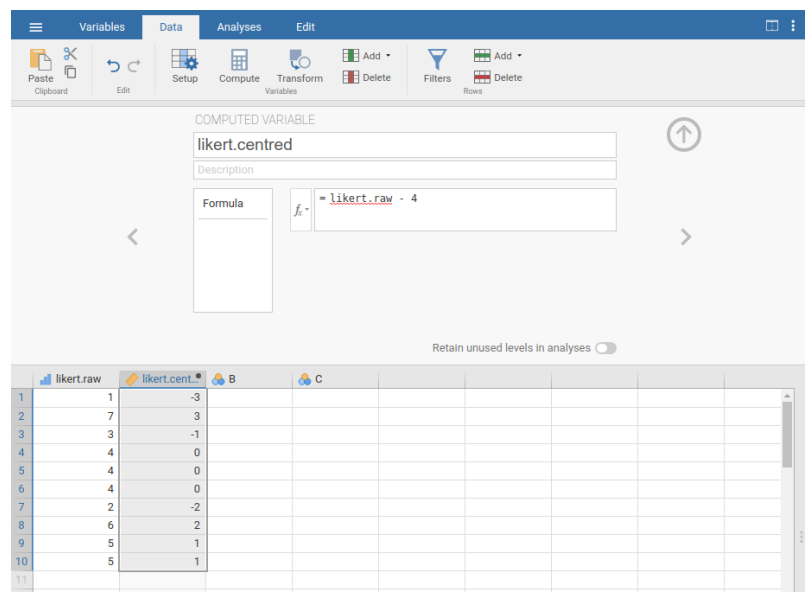
\includegraphics[width=0.9\linewidth]{images/Figure36} \caption{Creating a new computed variable in jamovi}\label{fig:fig6-4}
\end{figure}

One reason why it might be useful to have the data in this format is
that there are a lot of situations where you might prefer to analyse the
strength of the opinion separately from the direction of the opinion. We
can do two different transformations on this likert.centred variable in
order to distinguish between these two different concepts. First, to
compute an opinion.strength variable, we want to take the absolute value
of the centred data (using the `ABS' function).\footnote{The absolute value of a number is its distance from zero,
  regardless of whether it's sign is negative or positive.} In
jamovi, create another new variable using the `Compute' button. Name the
variable opinion.strength and this time click on the fx button next to
the `Formula' box. This shows the different `Functions' and `Variables'
that you can add to the `Formula' box, so double click on `ABS' and then
double click on ``likert.centred' and you will see that the `Formula' box
is populated with ABS(likert.centred) and a new variable has been
created in the spreadsheet view, as in Figure \ref{fig:fig6-5}.

\begin{figure}
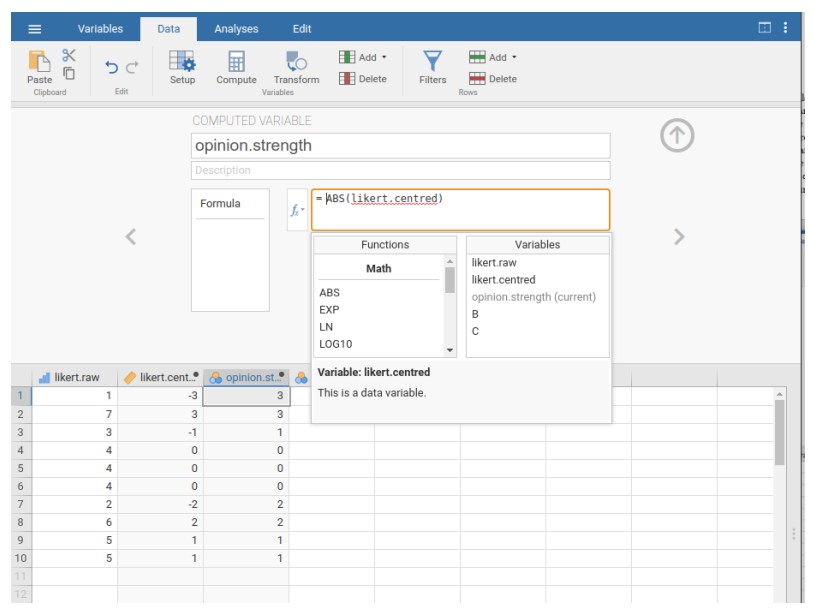
\includegraphics[width=0.9\linewidth]{images/Figure6_6} \caption{Using the $f_x$ button to select functions and variables}\label{fig:fig6-5}
\end{figure}

Second, to compute a variable that contains only the direction of the
opinion and ignores the strength, we want to calculate the `sign' of the
variable. In jamovi we can use the IF function to do this. Create
another new variable using the `Compute' button, name this one
opinion.sign, and then type the following into the function box:

IF(likert.centred \(==\) 0, 0, likert.centred / opinion.strength) When done,
you'll see that all negative numbers from the likert.centred variable
are converted to -1, all positive numbers are converted to 1 and zero
stays as 0, like so:

-1 1 -1 0 0 0 -1 1 1 1

Let's break down what this `IF' command is doing. In jamovi there are
three parts to an `IF' statement, written as 'IF(expression, value,
else)'. The first part, `expression' can be a logical or mathematical
statement. In our example, we have specified `likert.centred \(==\) 0',
which is TRUE for values where likert.centred is zero. The next part,
`value', is the new value where the expression in part one is TRUE. In
our example, we have said that for all those values where likert.centred
is zero, keep them zero. In the next part, `else', we can enter another
logical or mathematical statement to be used if part one evaluates to
FALSE, i.e.~where likert.centred is not zero. In our example we have
divided likert.centred by opinion.strength to give `-1' or `+1'
depending of the sign of the original value in
likert.centred.\footnote{The reason we have to use the `IF' command and keep zero as zero
  is that you cannot just use likert.centred / opinion.strength to
  calculate the sign of likert.centred, because mathematically dividing
  zero by zero does not work. Try it and see}

And we're done. We now have three shiny new variables, all of which are
useful transformations of the original likert.raw data.

\hypertarget{collapsing-a-variable-into-a-smaller-number-of-discrete-levels-or-categories}{%
\subsection{Collapsing a variable into a smaller number of discrete levels or categories}\label{collapsing-a-variable-into-a-smaller-number-of-discrete-levels-or-categories}}

One pragmatic task that comes up quite often is the problem of
collapsing a variable into a smaller number of discrete levels or
categories. For instance, suppose I'm interested in looking at the age
distribution of people at a social gathering:

60,58,24,26,34,42,31,30,33,2,9

In some situations it can be quite helpful to group these into a
smallish number of categories. For example, we could group the data into
three broad categories: young (0-20), adult (21-40) and older (41-60).
This is a quite coarse-grained classification, and the labels that I've
attached only make sense in the context of this data set (e.g., viewed
more generally, a 42 year old wouldn't consider themselves as ``older'').
We can slice this variable up quite easily using the jamovi `IF'
function that we have already used. This time we have to specify nested
`IF' statements, meaning simply that IF the first logical expression is
TRUE, insert a first value, but IF a second logical expression is TRUE,
insert a second value, but IF a third logical expression is TRUE, then
insert a third value. This can be written as:

IF(Age \textgreater= 0 and Age \textless= 20, 1, IF(Age \textgreater= 21 and Age \textless= 40, 2, IF(Age
\textgreater= 41 and Age \textless= 60, 3 )))

Note that there are three left parentheses used during the nesting, so
the whole statement has to end with three right parentheses otherwise
you will get an error message. The jamovi screen shot for this data
manipulation, along with an accompanying frequency table, is shown in
Figure \ref{fig:fig6-6}.

\begin{figure}
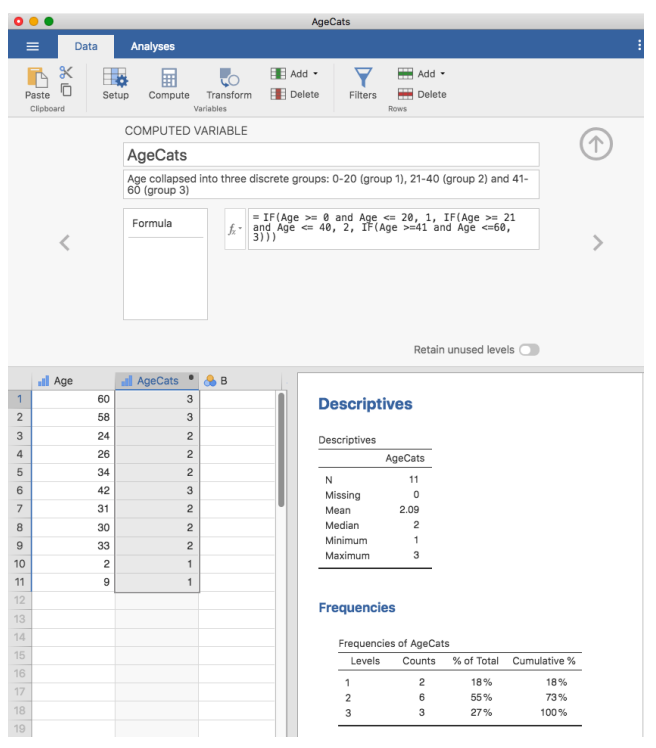
\includegraphics[width=0.9\linewidth]{images/Figure40} \caption{Collapsing a variable into a smaller number of discrete levels using the jamovi ‘IF’ function}\label{fig:fig6-6}
\end{figure}

It's important to take the time to figure out whether or not the
resulting categories make any sense at all in terms of your research
project. If they don't make any sense to you as meaningful categories,
then any data analysis that uses those categories is likely to be just
as meaningless. More generally, in practice I've noticed that people
have a very strong desire to carve their (continuous and messy) data
into a few (discrete and simple) categories, and then run analyses using
the categorised data instead of the original data.\footnote{If you've read further into the book, and are re-reading this
  section, then a good example of this would be someone choosing to do an
  ANOVA using AgeCats as the grouping variable, instead of running a
  regression using Age as a predictor. There are sometimes good reasons
  for doing this. For instance, if the relationship between Age and your
  outcome variable is highly non-linear and you aren't comfortable with
  trying to run non-linear regression! However, unless you really do have
  a good rationale for doing this, it's best not to. It tends to introduce
  all sorts of other problems (e.g., the data will probably violate the
  normality assumption) and you can lose a lot of statistical power.} I
wouldn't go so far as to say that this is an inherently bad idea, but it
does have some fairly serious drawbacks at times, so I would advise some
caution if you are thinking about doing it.

\hypertarget{creating-a-transformation-that-can-be-applied-to-multiple-variables}{%
\subsection{Creating a transformation that can be applied to multiple variables}\label{creating-a-transformation-that-can-be-applied-to-multiple-variables}}

Sometimes you want to apply the same transformation to more than one
variable, for example when you have multiple questionnaire items that
all need to be recalculated or recoded in the same way. And one of the
neat features in jamovi is that you can create a transformation, using
the `Data' - `Transform' button, that can then be saved and applied to
multiple variables. Let's go back to the first example above, using the
data file likert.omv that contains a single variable with raw
Likert-scale responses for 10 people. To create a transformation that
you can save and then apply across multiple variables (assuming you had
more variables like this in your data file), first in the spreadsheet
editor select (i.e., click) the variable you want to use to initially
create the transformation. In our example this is likert.raw. Next click
the `Transform' button in the jamovi `Data' ribbon, and you'll see
something like Figure \ref{fig:fig6-7}.

Give your new variable a name, let's call it opinion.strength and then
click on the `using transform' selection box and select `Create New
Transform\ldots{}'. This is where you will create, and name, the
transformation that can be re-applied to as many variables as you like.
The transformation is automatically named for us as `Transform 1'
(imaginative, huh. You can change this if you like). Then type the
expression ``ABS(\$source - 4)'' into the function text box, as in Figure \ref{fig:fig6-8}, press Enter or Return on your keyboard and, hey presto, you
have created a new transformation and applied it to the likert.raw
variable! Good, eh. Note that instead of using the variable label in the
expression, we have instead used `\$source'. This is so that we can then
use the same transformation with as many different variables as we
like - jamovi requires you to use `\$source' to refer to the source
variable you are transforming. Your transformation has also been saved
and can be re-used any time you like (providing you save the dataset as
an `.omv' file, otherwise you'll lose it!).

You can also create a transformation with the second example we looked
at, the age distribution of people at a social gathering. Go on, you
know you want to! Remember that we collapsed this variable into three
groups: younger, adult and older. This time we will achieve the same
thing, but using the jamovi `Transform' - `Add condition' button. With
this data set (go back to it or create it again if you didn't save it)
set up a new variable transformation. Call the transformed variable
AgeCats and the transformation you will create Agegroupings. Then click
on the big ``\(+\)'' sign next to the function box. This is the `Add
condition' button and I've stuck a big red arrow onto Figure \ref{fig:fig6-9} so
you can see exactly where this is. Re-create the transformation shown in
Figure \ref{fig:fig6-9} and when you have done, you will see the new values
appear in the spreadsheet window. What's more, the Age groupings
transformation has been saved and can be re-applied any time you like.
Ok, so I know that it's unlikely you will have more than one `Age'
variable, but you get the idea now of how to set up transformations in
jamovi, so you can follow this idea with other sorts of variables. A
typical scenario for this is when you have a questionnaire scale with,
say, 20 items (variables) and each item was originally scored from 1 to
6 but, for some reason or quirk of the data you decide to recode all the
items as 1 to 3. You can easily do this in jamovi by creating and then
re-applying your transformation for each variable that you want to
recode.

\begin{figure}
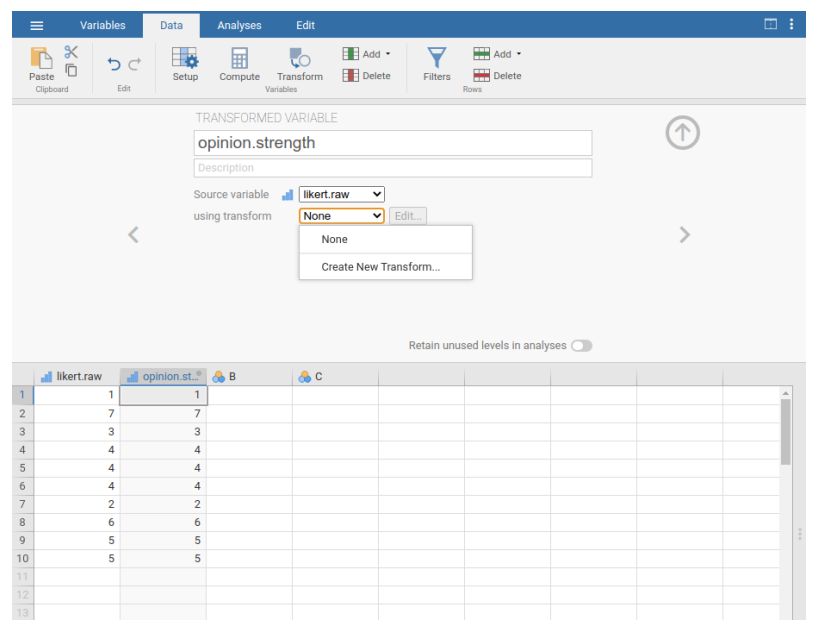
\includegraphics[width=0.9\linewidth]{images/Figure38} \caption{Creating a new variable transformation using the jamovi ‘Transform’ command}\label{fig:fig6-7}
\end{figure}

\begin{figure}
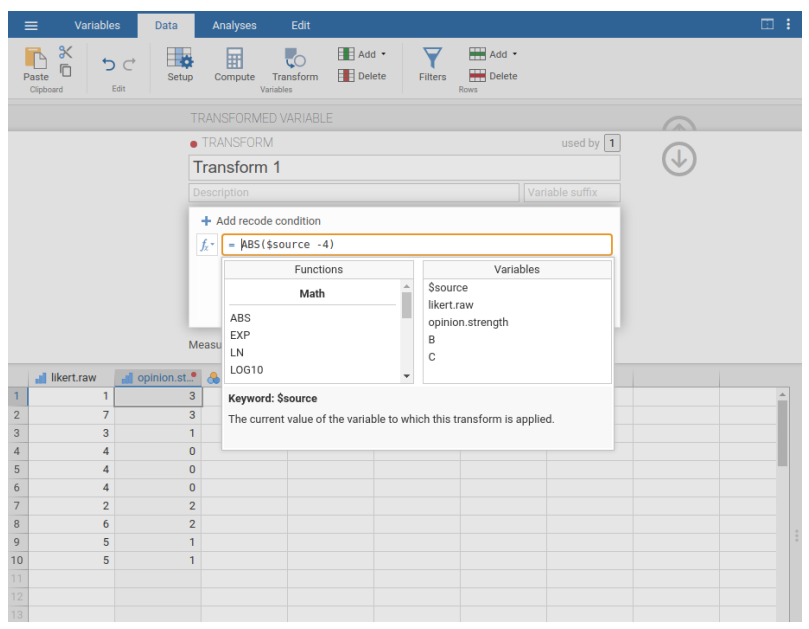
\includegraphics[width=0.9\linewidth]{images/Figure39} \caption{Specifying a transformation in jamovi, to be saved as the imaginatively named ‘Transform 1’}\label{fig:fig6-8}
\end{figure}

\begin{figure}
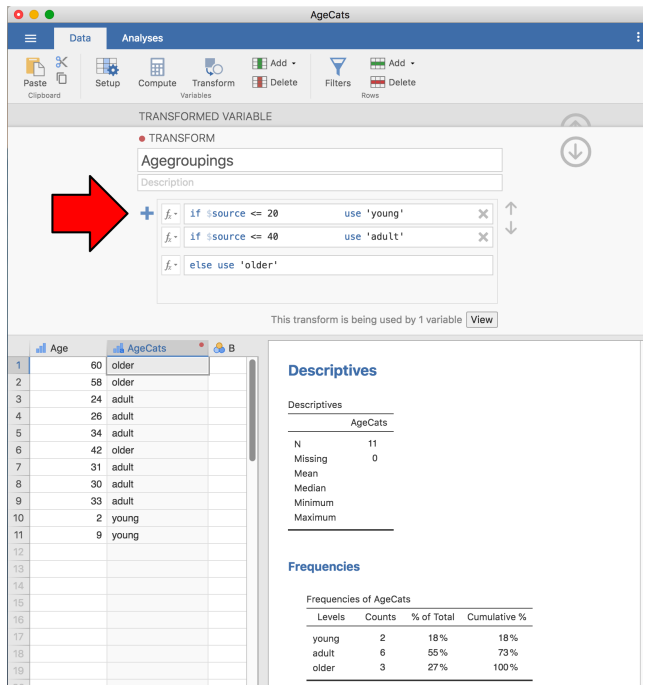
\includegraphics[width=0.9\linewidth]{images/Figure41} \caption{jamovi transformation into three age categories, using the ‘Add condition’ button}\label{fig:fig6-9}
\end{figure}

 
  \providecommand{\huxb}[2]{\arrayrulecolor[RGB]{#1}\global\arrayrulewidth=#2pt}
  \providecommand{\huxvb}[2]{\color[RGB]{#1}\vrule width #2pt}
  \providecommand{\huxtpad}[1]{\rule{0pt}{#1}}
  \providecommand{\huxbpad}[1]{\rule[-#1]{0pt}{#1}}

\begin{table}[ht]
\begin{centerbox}
\begin{threeparttable}
\setlength{\tabcolsep}{0pt}
\begin{tabular}{l l l l}


\hhline{>{\huxb{0, 0, 0}{0.4}}->{\huxb{0, 0, 0}{0.4}}->{\huxb{0, 0, 0}{0.4}}->{\huxb{0, 0, 0}{0.4}}-}
\arrayrulecolor{black}

\multicolumn{1}{!{\huxvb{0, 0, 0}{0}}c!{\huxvb{0, 0, 0}{0}}}{\cellcolor[RGB]{242, 242, 242}\huxtpad{6pt + 1em}\centering \hspace{0pt} \textbf{} \hspace{6pt}\huxbpad{6pt}} &
\multicolumn{1}{c!{\huxvb{0, 0, 0}{0}}}{\cellcolor[RGB]{242, 242, 242}\huxtpad{6pt + 1em}\centering \hspace{6pt} \textbf{function} \hspace{6pt}\huxbpad{6pt}} &
\multicolumn{1}{c!{\huxvb{0, 0, 0}{0}}}{\cellcolor[RGB]{242, 242, 242}\huxtpad{6pt + 1em}\centering \hspace{6pt} \textbf{example input} \hspace{6pt}\huxbpad{6pt}} &
\multicolumn{1}{c!{\huxvb{0, 0, 0}{0}}}{\cellcolor[RGB]{242, 242, 242}\huxtpad{6pt + 1em}\centering \hspace{6pt} \textbf{(answer)} \hspace{0pt}\huxbpad{6pt}} \tabularnewline[-0.5pt]


\hhline{>{\huxb{0, 0, 0}{0.4}}->{\huxb{0, 0, 0}{0.4}}->{\huxb{0, 0, 0}{0.4}}->{\huxb{0, 0, 0}{0.4}}-}
\arrayrulecolor{black}

\multicolumn{1}{!{\huxvb{0, 0, 0}{0}}c!{\huxvb{0, 0, 0}{0}}}{\huxtpad{6pt + 1em}\centering \hspace{0pt} square root \hspace{6pt}\huxbpad{6pt}} &
\multicolumn{1}{c!{\huxvb{0, 0, 0}{0}}}{\huxtpad{6pt + 1em}\centering \hspace{6pt} SQRT(x) \hspace{6pt}\huxbpad{6pt}} &
\multicolumn{1}{c!{\huxvb{0, 0, 0}{0}}}{\huxtpad{6pt + 1em}\centering \hspace{6pt} SQRT(25) \hspace{6pt}\huxbpad{6pt}} &
\multicolumn{1}{c!{\huxvb{0, 0, 0}{0}}}{\huxtpad{6pt + 1em}\centering \hspace{6pt} 5 \hspace{0pt}\huxbpad{6pt}} \tabularnewline[-0.5pt]


\hhline{}
\arrayrulecolor{black}

\multicolumn{1}{!{\huxvb{0, 0, 0}{0}}c!{\huxvb{0, 0, 0}{0}}}{\cellcolor[RGB]{242, 242, 242}\huxtpad{6pt + 1em}\centering \hspace{0pt} absolute value \hspace{6pt}\huxbpad{6pt}} &
\multicolumn{1}{c!{\huxvb{0, 0, 0}{0}}}{\cellcolor[RGB]{242, 242, 242}\huxtpad{6pt + 1em}\centering \hspace{6pt} ABS(x) \hspace{6pt}\huxbpad{6pt}} &
\multicolumn{1}{c!{\huxvb{0, 0, 0}{0}}}{\cellcolor[RGB]{242, 242, 242}\huxtpad{6pt + 1em}\centering \hspace{6pt} ABS(-23) \hspace{6pt}\huxbpad{6pt}} &
\multicolumn{1}{c!{\huxvb{0, 0, 0}{0}}}{\cellcolor[RGB]{242, 242, 242}\huxtpad{6pt + 1em}\centering \hspace{6pt} 23 \hspace{0pt}\huxbpad{6pt}} \tabularnewline[-0.5pt]


\hhline{}
\arrayrulecolor{black}

\multicolumn{1}{!{\huxvb{0, 0, 0}{0}}c!{\huxvb{0, 0, 0}{0}}}{\huxtpad{6pt + 1em}\centering \hspace{0pt} logarithm (base 10) \hspace{6pt}\huxbpad{6pt}} &
\multicolumn{1}{c!{\huxvb{0, 0, 0}{0}}}{\huxtpad{6pt + 1em}\centering \hspace{6pt} LOG10(x) \hspace{6pt}\huxbpad{6pt}} &
\multicolumn{1}{c!{\huxvb{0, 0, 0}{0}}}{\huxtpad{6pt + 1em}\centering \hspace{6pt} LOG10(1000) \hspace{6pt}\huxbpad{6pt}} &
\multicolumn{1}{c!{\huxvb{0, 0, 0}{0}}}{\huxtpad{6pt + 1em}\centering \hspace{6pt} 3 \hspace{0pt}\huxbpad{6pt}} \tabularnewline[-0.5pt]


\hhline{}
\arrayrulecolor{black}

\multicolumn{1}{!{\huxvb{0, 0, 0}{0}}c!{\huxvb{0, 0, 0}{0}}}{\cellcolor[RGB]{242, 242, 242}\huxtpad{6pt + 1em}\centering \hspace{0pt} logarithm (base e) \hspace{6pt}\huxbpad{6pt}} &
\multicolumn{1}{c!{\huxvb{0, 0, 0}{0}}}{\cellcolor[RGB]{242, 242, 242}\huxtpad{6pt + 1em}\centering \hspace{6pt} LN(x) \hspace{6pt}\huxbpad{6pt}} &
\multicolumn{1}{c!{\huxvb{0, 0, 0}{0}}}{\cellcolor[RGB]{242, 242, 242}\huxtpad{6pt + 1em}\centering \hspace{6pt} LN(1000) \hspace{6pt}\huxbpad{6pt}} &
\multicolumn{1}{c!{\huxvb{0, 0, 0}{0}}}{\cellcolor[RGB]{242, 242, 242}\huxtpad{6pt + 1em}\centering \hspace{6pt} 6.91 \hspace{0pt}\huxbpad{6pt}} \tabularnewline[-0.5pt]


\hhline{}
\arrayrulecolor{black}

\multicolumn{1}{!{\huxvb{0, 0, 0}{0}}c!{\huxvb{0, 0, 0}{0}}}{\huxtpad{6pt + 1em}\centering \hspace{0pt} exponentiation \hspace{6pt}\huxbpad{6pt}} &
\multicolumn{1}{c!{\huxvb{0, 0, 0}{0}}}{\huxtpad{6pt + 1em}\centering \hspace{6pt} EXP(x) \hspace{6pt}\huxbpad{6pt}} &
\multicolumn{1}{c!{\huxvb{0, 0, 0}{0}}}{\huxtpad{6pt + 1em}\centering \hspace{6pt} EXP(6.908) \hspace{6pt}\huxbpad{6pt}} &
\multicolumn{1}{c!{\huxvb{0, 0, 0}{0}}}{\huxtpad{6pt + 1em}\centering \hspace{6pt} 1e+03 \hspace{0pt}\huxbpad{6pt}} \tabularnewline[-0.5pt]


\hhline{}
\arrayrulecolor{black}

\multicolumn{1}{!{\huxvb{0, 0, 0}{0}}c!{\huxvb{0, 0, 0}{0}}}{\cellcolor[RGB]{242, 242, 242}\huxtpad{6pt + 1em}\centering \hspace{0pt} box-cox \hspace{6pt}\huxbpad{6pt}} &
\multicolumn{1}{c!{\huxvb{0, 0, 0}{0}}}{\cellcolor[RGB]{242, 242, 242}\huxtpad{6pt + 1em}\centering \hspace{6pt} BOXCOX(x, lamda) \hspace{6pt}\huxbpad{6pt}} &
\multicolumn{1}{c!{\huxvb{0, 0, 0}{0}}}{\cellcolor[RGB]{242, 242, 242}\huxtpad{6pt + 1em}\centering \hspace{6pt} BOXCOX(6.908, 3) \hspace{6pt}\huxbpad{6pt}} &
\multicolumn{1}{c!{\huxvb{0, 0, 0}{0}}}{\cellcolor[RGB]{242, 242, 242}\huxtpad{6pt + 1em}\centering \hspace{6pt} 110 \hspace{0pt}\huxbpad{6pt}} \tabularnewline[-0.5pt]


\hhline{>{\huxb{0, 0, 0}{0.4}}->{\huxb{0, 0, 0}{0.4}}->{\huxb{0, 0, 0}{0.4}}->{\huxb{0, 0, 0}{0.4}}-}
\arrayrulecolor{black}
\end{tabular}\captionsetup{justification=raggedright,singlelinecheck=off}
\caption{\label{tab:tab6-5} Some mathematical operators}
 
\end{threeparttable}\par\end{centerbox}

\end{table}
 

\hypertarget{a-few-more-mathematical-functions-and-operations}{%
\section{A few more mathematical functions and operations}\label{a-few-more-mathematical-functions-and-operations}}

In Section \textbf{6.3} I discussed the ideas behind variable transformations
and showed that a lot of the transformations that you might want to
apply to your data are based on fairly simple mathematical functions and
operations. In this section I want to return to that discussion and
mention several other mathematical functions and arithmetic operations
that are actually quite useful for a lot of real world data analysis.
Table \ref{tab:tab6-5} gives a brief overview of the various mathematical
functions I want to talk about here, or later.\footnote{We'll leave the box-cox function until later on} Obviously
this doesn't even come close to cataloguing the range of possibilities
available, but it does cover a range of functions that are used
regularly in data analysis and that are available in jamovi.

\hypertarget{logarithms-and-exponentials}{%
\subsection{Logarithms and exponentials}\label{logarithms-and-exponentials}}

As I've mentioned earlier, jamovi has an useful range of mathematical
functions built into it and there really wouldn't be much point in
trying to describe or even list all of them. For the most part, I've
focused only on those functions that are strictly necessary for this
book. However I do want to make an exception for logarithms and
exponentials. Although they aren't needed anywhere else in this book,
they are \emph{everywhere} in statistics more broadly. And not only that,
there are a \emph{lot of} situations in which it is convenient to analyse the
logarithm of a variable (i.e., to take a ``log-transform'' of the
variable). I suspect that many (maybe most) readers of this book will
have encountered logarithms and exponentials before, but from past
experience I know that there's a substantial proportion of students who
take a social science statistics class who haven't touched logarithms
since high school, and would appreciate a bit of a refresher.

In order to understand logarithms and exponentials, the easiest thing to
do is to actually calculate them and see how they relate to other simple
calculations. There are three jamovi functions in particular that I want
to talk about, namely LN(), LOG10() and EXP(). To start with, let's
consider LOG10(), which is known as the ``logarithm in base 10''. The
trick to understanding a \textbf{logarithm} is to understand that it's
basically the ``opposite'' of taking a power. Specifically, the logarithm
in base 10 is closely related to the powers of 10. So let's start by
noting that 10-cubed is 1000. Mathematically, we would write this:

\[10^3=1000\]

The trick to understanding a logarithm is to recognise that the
statement that ``10 to the power of 3 is equal to 1000'' is equivalent to
the statement that ``the logarithm (in base 10) of 1000 is equal to 3''.
Mathematically, we write this as follows,

\[log_{10}(1000)=3\]

Okay, since the LOG10() function is related to the powers of 10, you
might expect that there are other logarithms (in bases other than 10)
that are related to other powers too. And of course that's true: there's
not really anything mathematically special about the number 10. You and
I happen to find it useful because decimal numbers are built around the
number 10, but the big bad world of mathematics scoffs at our decimal
numbers. Sadly, the universe doesn't actually care how we write down
numbers. Anyway, the consequence of this cosmic indifference is that
there's nothing particularly special about calculating logarithms in
base 10. You could, for instance, calculate your logarithms in base 2.
Alternatively, a third type of logarithm, and one we see a lot more of
in statistics than either base 10 or base 2, is called the \textbf{natural
logarithm}, and corresponds to the logarithm in base e. Since you might
one day run into it, I'd better explain what e is. The number e, known
as \textbf{Euler's number}, is one of those annoying ``irrational'' numbers
whose decimal expansion is infinitely long, and is considered one of the
most important numbers in mathematics. The first few digits of e are:

\[e = 2.718282 \]

There are quite a few situation in statistics that require us to
calculate powers of \(e\), though none of them appear in this book.
Raising e to the power \(x\) is called the \textbf{exponential} of \(x\),
and so it's very common to see \(e^x\) written as exppxq. And so it's
no surprise that jamovi has a function that calculates exponentials,
called EXP(). Because the number e crops up so often in statistics, the
natural logarithm (i.e., logarithm in base e) also tends to turn up.
Mathematicians often write it as \(log_e(x)\) or \(ln(x)\). In fact,
jamovi works the same way: the LN() function corresponds to the natural
logarithm.

And with that, I think we've had quite enough exponentials and
logarithms for this book!

\hypertarget{extracting-a-subset-of-the-data}{%
\section{Extracting a subset of the data}\label{extracting-a-subset-of-the-data}}

One very important kind of data handling is being able to extract a
particular subset of the data. For instance, you might be interested
only in analysing the data from one experimental condition, or you may
want to look closely at the data from people over 50 years in age. To do
this, the first step is getting jamovi to filter the subset of the data
corresponding to the observations that you're interested in.

This section returns to the nightgarden.csv data set. If you're reading
this whole chapter in one sitting, then you should already have this
data set loaded into a jamovi window. For this section, let's focus on
the two variables speaker and utterance (see Section \textbf{6.1} if you've
forgotten what those variables look like). Suppose that what I want to
do is pull out only those utterances that were made by Makka-Pakka. To
that end, we need to specify a filter in jamovi. First open up a filter
window by clicking on `Filters' on the main jamovi `Data' toolbar. Then,
in the `Filter 1' text box, next to the `=' sign, type the following:

speaker == 'makka-pakka'

\begin{figure}
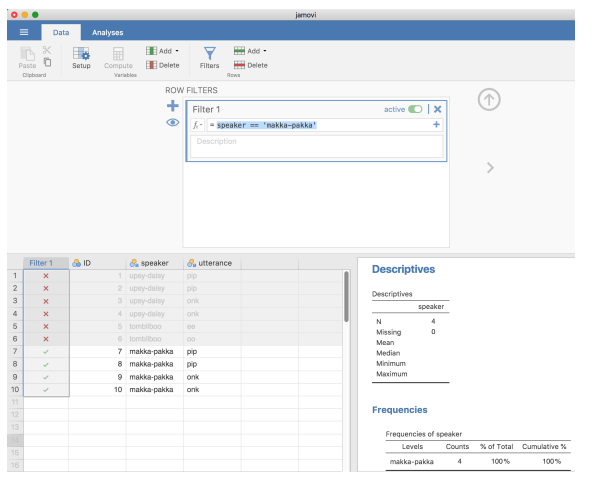
\includegraphics[width=0.9\linewidth]{images/Figure42} \caption{Creating a subset of the nightgarden data using the jamovi ‘Filters’ option}\label{fig:fig6-10}
\end{figure}

When you have done this, you will see that a new column has been added
to the spreadsheet window (see Figure \ref{fig:fig6-10}), labelled `Filter 1',
with the cases where speaker is not `makka-pakka' greyed-out
(i.e., filtered out) and, conversely, the cases where speaker is
`makka-pakka' have a green check mark indicating they are filtered in.
You can test this by running `Exploration' - `Descriptives' - `Frequency
tables' for the speaker variable and seeing what that shows. Go on, try
it!

Following on from this simple example, you can also build up more
complex filters using logical expressions in jamovi. For instance,
suppose I wanted to keep only those cases when the utterance is either
``pip'' or ``oo''. In this case in the `Filter 1' text box, next to the `='
sign, you would type the following:

utterance == 'pip' or utterance == 'oo'

\hypertarget{summary-4}{%
\section{Summary}\label{summary-4}}

Obviously, there's no real coherence to this chapter. It's just a grab
bag of topics and tricks that can be handy to know about, so the best
wrap up I can give here is just to repeat this list:

\begin{itemize}
\tightlist
\item
  \protect\hyperlink{tabulating-and-cross-tabulating-data}{Tabulating and cross-tabulating data}
\item
  \protect\hyperlink{logical-expressions-in-jamovi}{Logical expressions in jamovi}
\item
  \protect\hyperlink{transforming-and-recoding-a-variable}{Transforming and recoding a variable}
\item
  \protect\hyperlink{a-few-more-mathematical-functions-and-operations}{A few more mathematical functions and operations}
\item
  \protect\hyperlink{extracting-a-subset-of-the-data}{Extracting a subset of the data}
\end{itemize}

\begin{center}\rule{0.5\linewidth}{0.5pt}\end{center}

\hypertarget{prelude-to-part-iv}{%
\chapter*{Prelude to Part IV}\label{prelude-to-part-iv}}
\addcontentsline{toc}{chapter}{Prelude to Part IV}

Part IV of the book is by far the most theoretical, focusing as it does
on the theory of statistical inference. Over the next three chapters my
goal is to give you an \protect\hyperlink{introduction-to-probability}{Introduction to probability} theory, sampling and estimation in the chapter on {[}Estimating unknown quantities from a sample{]} and statistical \protect\hyperlink{hypothesis-testing}{Hypothesis testing}. Before we get started though, I want
to say something about the big picture. Statistical inference is
primarily about learning from data. The goal is no longer merely to
describe our data but to use the data to draw conclusions about the
world. To motivate the discussion I want to spend a bit of time talking
about a philosophical puzzle known as the riddle of induction, because
it speaks to an issue that will pop up over and over again throughout
the book: statistical inference relies on assumptions. This sounds like
a bad thing. In everyday life people say things like ``you should never
make assumptions'', and psychology classes often talk about assumptions
and biases as bad things that we should try to avoid. From bitter
personal experience I have learned never to say such things around
philosophers!

\hypertarget{on-the-limits-of-logical-reasoning}{%
\section*{On the limits of logical reasoning}\label{on-the-limits-of-logical-reasoning}}
\addcontentsline{toc}{section}{On the limits of logical reasoning}

\begin{quote}
\emph{The whole art of war consists in getting at what is on the other side
of the hill, or, in other words, in learning what we do not know from
what we do.}\\
- Arthur Wellesley, 1st Duke of Wellington
\end{quote}

I am told that quote above came about as a consequence of a carriage
ride across the countryside.\footnote{\href{\%0A\%20http://www.bartleby.com/344/400.html}{http://www.bartleby.com/344/400.html}} He and his companion, J.
W. Croker, were playing a guessing game, each trying to predict what
would be on the other side of each hill. In every case it turned out
that Wellesley was right and Croker was wrong. Many years later when
Wellesley was asked about the game he explained that ``the whole art of
war consists in getting at what is on the other side of the hill''.
Indeed, war is not special in this respect. All of life is a guessing
game of one form or another, and getting by on a day to day basis
requires us to make good guesses. So let's play a guessing game of our
own.

Suppose you and I are observing the Wellesley-Croker competition and
after every three hills you and I have to predict who will win the next
one, Wellesley or Croker. Let's say that W refers to a Wellesley victory
and C refers to a Croker victory. After three hills, our data set looks
like this:

\(WWW\)

Our conversation goes like this:

\begin{quote}
you: Three in a row doesn't mean much. I suppose Wellesley might be
better at this than Croker, but it might just be luck. Still, I'm a bit
of a gambler. I'll bet on Wellesley.
\end{quote}

\begin{quote}
me: I agree that three in a row isn't informative and I see no reason to prefer Wellesley's guesses over
Croker's. I can't justify betting at this stage. Sorry. No bet for me.
\end{quote}

Your gamble paid off: three more hills go by and Wellesley wins all three. Going into the next round of our game the score is 1-0 in favour of you and our data set looks like this: \(WWW\) \(WWW\) I've organised the data into blocks of three so that you can see which batch corresponds to the observations that we had available at each step in our little side game. After seeing this new batch, our conversation continues:

\begin{quote}
you: Six wins in a row for Duke Wellesley. This is starting to feel a
bit suspicious. I'm still not certain, but I reckon that he's going to
win the next one too.
\end{quote}

\begin{quote}
me: I guess I don't see that. Sure, I agree that
Wellesley has won six in a row, but I don't see any logical reason why
that means he'll win the seventh one. No bet. you: Do you really think
so? Fair enough, but my bet worked out last time and I'm okay with my
choice.
\end{quote}

For a second time you were right, and for a second time I was wrong. Wellesley wins the next three hills, extending his winning record against Croker to 9-0. The data set available to us is now this: \(WWW\) \(WWW\) \(WWW\) And our conversation goes like this:

\begin{quote}
you: Okay, this is pretty obvious. Wellesley is way better at this game.
We both agree he's going to win the next hill, right?
\end{quote}

\begin{quote}
me: Is there
really any logical evidence for that? Before we started this game, there
were lots of possibilities for the first 10 outcomes, and I had no idea
which one to expect. \(WWW\) \(WWW\) \(WWW\) \(W\) was one possibility, but so was \(WCC\)
\(CWC\) \(WWC\) \(C\) and \(WWW\) \(WWW\) \(WWW\) \(C\) or even \(CCC\) \(CCC\) \(CCC\) \(C\). Because I had no idea
what would happen so I'd have said they were all equally likely. I
assume you would have too, right? I mean, that's what it means to say
you have ``no idea'', isn't it?
\end{quote}

\begin{quote}
you: I suppose so.
\end{quote}

\begin{quote}
me: Well then, the
observations we've made logically rule out all possibilities except two:
\(WWW\) \(WWW\) \(WWW\) \(C\) or \(WWW\) \(WWW\) \(WWW\) \(W\). Both of these are perfectly consistent
with the evidence we've encountered so far, aren't they?
\end{quote}

\begin{quote}
you: Yes, of
course they are. Where are you going with this? me: So what's changed
then? At the start of our game, you'd have agreed with me that these are
equally plausible and none of the evidence that we've encountered has
discriminated between these two possibilities. Therefore, both of these
possibilities remain equally plausible and I see no logical reason to
prefer one over the other. So yes, while I agree with you that
Wellesley's run of 9 wins in a row is remarkable, I can't think of a
good reason to think he'll win the 10th hill. No bet.
\end{quote}

\begin{quote}
you: I see your point, but I'm still willing to chance it. I'm betting on Wellesley.
\end{quote}

Wellesley's winning streak continues for the next three hills. The score in the Wellesley-Croker game is now 12-0, and the score in our game is now 3-0. As we approach the fourth round of our game, our data set is this: \(WWW\) \(WWW\) \(WWW\) \(WWW\) and the conversation continues:

\begin{quote}
you: Oh yeah! Three more wins for Wellesley and another victory for me.
Admit it, I was right about him! I guess we're both betting on Wellesley
this time around, right?
\end{quote}

\begin{quote}
me: I don't know what to think. I feel like
we're in the same situation we were in last round, and nothing much has
changed. There are only two legitimate possibilities for a sequence of
13 hills that haven't already been ruled out, \(WWW\) \(WWW\) \(WWW\) \(WWW\) \(C\) and \(WWW\)
\(WWW\) \(WWW\) \(WWW\) \(W\). It's just like I said last time. If all possible outcomes
were equally sensible before the game started, shouldn't these two be
equally sensible now given that our observations don't rule out either
one? I agree that it feels like Wellesley is on an amazing winning
streak, but where's the logical evidence that the streak will continue?
\end{quote}

\begin{quote}
you: I think you're being unreasonable. Why not take a look at our
scorecard, if you need evidence? You're the expert on statistics and
you've been using this fancy logical analysis, but the fact is you're
losing. I'm just relying on common sense and I'm winning. Maybe you
should switch strategies.
\end{quote}

\begin{quote}
me: Hmm, that is a good point and I don't want
to lose the game, but I'm afraid I don't see any logical evidence that
your strategy is better than mine. It seems to me that if there were
someone else watching our game, what they'd have observed is a run of
three wins to you. Their data would look like this: \(YYY\). Logically, I
don't see that this is any different to our first round of watching
Wellesley and Croker. Three wins to you doesn't seem like a lot of
evidence, and I see no reason to think that your strategy is working out
any better than mine. If I didn't think that \(WWW\) was good evidence then
for Wellesley being better than Croker at their game, surely I have no
reason now to think that YYY is good evidence that you're better at
ours?
\end{quote}

\begin{quote}
you: Okay, now I think you're being a jerk.
\end{quote}

\begin{quote}
me: I don't see the logical evidence for that.
\end{quote}

\hypertarget{learning-without-making-assumptions-is-a-myth}{%
\section*{Learning without making assumptions is a myth}\label{learning-without-making-assumptions-is-a-myth}}
\addcontentsline{toc}{section}{Learning without making assumptions is a myth}

There are lots of different ways in which we could dissect this
dialogue, but since this is a statistics book pitched at psychologists
and not an introduction to the philosophy and psychology of reasoning,
I'll keep it brief. What I've described above is sometimes referred to
as the riddle of induction. It seems entirely reasonable to think that a
12-0 winning record by Wellesley is pretty strong evidence that he will
win the 13th game, but it is not easy to provide a proper logical
justification for this belief. On the contrary, despite the obviousness
of the answer, it's not actually possible to justify betting on
Wellesley without relying on some assumption that you don't have any
logical justification for.

The riddle of induction is most associated with the philosophical work
of David Hume and more recently Nelson Goodman, but you can find
examples of the problem popping up in fields as diverse as literature
(Lewis Carroll) and machine learning (the ``no free lunch'' theorem).
There really is something weird about trying to ``learn what we do not
know from what we do know''. The critical point is that assumptions and
biases are unavoidable if you want to learn anything about the world.
There is no escape from this, and it is just as true for statistical
inference as it is for human reasoning. In the dialogue I was taking aim
at your perfectly sensible inferences as a human being, but the common
sense reasoning that you relied on is no different to what a
statistician would have done. Your ``common sense'' half of the dialog
relied on an implicit assumption that there exists some difference in
skill between Wellesley and Croker, and what you were doing was trying
to work out what that difference in skill level would be. My ``logical
analysis'' rejects that assumption entirely. All I was willing to accept
is that there are sequences of wins and losses and that I did not know
which sequences would be observed. Throughout the dialogue I kept
insisting that all logically possible data sets were equally plausible
at the start of the Wellesely-Croker game, and the only way in which I
ever revised my beliefs was to eliminate those possibilities that were
factually inconsistent with the observations.

That sounds perfectly sensible on its own terms. In fact, it even sounds
like the hallmark of good deductive reasoning. Like Sherlock Holmes, my
approach was to rule out that which is impossible in the hope that what
would be left is the truth. Yet as we saw, ruling out the impossible
never led me to make a prediction. On its own terms everything I said in
my half of the dialogue was entirely correct. An inability to make any
predictions is the logical consequence of making ``no assumptions''. In
the end I lost our game because you did make some assumptions and those
assumptions turned out to be right. Skill is a real thing, and because
you believed in the existence of skill you were able to learn that
Wellesley had more of it than Croker. Had you relied on a less sensible
assumption to drive your learning you might not have won the game.

Ultimately there are two things you should take away from this. First,
as I've said, you cannot avoid making assumptions if you want to learn
anything from your data. But second, once you realise that assumptions
are necessary it becomes important to make sure you make the right ones!
A data analysis that relies on few assumptions is not necessarily better
than one that makes many assumptions, it all depends on whether those
assumptions are good ones for your data. As we go through the rest of
this book I'll often point out the assumptions that underpin a
particular statistical technique, and how you can check whether those
assumptions are sensible.

\begin{center}\rule{0.5\linewidth}{0.5pt}\end{center}

\hypertarget{introduction-to-probability}{%
\chapter{Introduction to probability}\label{introduction-to-probability}}

\begin{quote}
\emph{{[}God{]} has afforded us only the twilight \ldots{} of Probability.}\\
- John Locke
\end{quote}

Up to this point in the book we've discussed some of the key ideas in experimental design, and we've talked a little about how you can summarise a data set. To a lot of people this is all there is to statistics: collecting all the numbers, calculating averages, drawing pictures, and putting them all in a report somewhere. Kind of like stamp collecting but with numbers. However, statistics covers much more than that. In fact, descriptive statistics is one of the smallest parts of statistics and one of the least powerful. The bigger and more useful part of statistics is that it provides information that lets you make inferences about data.

Once you start thinking about statistics in these terms, that statistics is there to help us draw inferences from data, you start seeing examples of it everywhere. For instance, here's a tiny extract from a newspaper article in the Sydney Morning Herald (30 Oct 2010):

\begin{quote}
``I have a tough job,'' the Premier said in response to a poll which found her government is now the most unpopular Labor administration in polling history, with a primary vote of just 23 per cent.
\end{quote}

This kind of remark is entirely unremarkable in the papers or in everyday life, but let's have a think about what it entails. A polling company has conducted a survey, usually a pretty big one because they can afford it. I'm too lazy to track down the original survey so let's just imagine that they called 1000 New South Wales (NSW) voters at random, and 230 (23\%) of those claimed that they intended to vote for the Australian Labor Party (ALP). For the 2010 Federal election the Australian Electoral Commission reported 4,610,795 enrolled voters in NSW, so the opinions of the remaining 4,609,795 voters (about 99.98\% of voters) remain unknown to us. Even assuming that no-one lied to the polling company the only thing we can say with 100\% confidence is that the true ALP primary vote is somewhere between 230/4610795 (about 0.005\%) and 4610025/4610795 (about 99.83\%). So, on what basis is it legitimate for the polling company, the newspaper, and the readership to conclude that the ALP primary vote is only about 23\%?

The answer to the question is pretty obvious. If I call 1000 people at random, and 230 of them say they intend to vote for the ALP, then it seems very unlikely that these are the only 230 people out of the entire voting public who actually intend to vote ALP. In other words, we assume that the data collected by the polling company is pretty representative of the population at large. But how representative? Would we be surprised to discover that the true ALP primary vote is actually 24\%? 29\%? 37\%? At this point everyday intuition starts to break down a bit. No-one would be surprised by 24\%, and everybody would be surprised by 37\%, but it's a bit hard to say whether 29\% is plausible. We need some more powerful tools than just looking at the numbers and guessing.

\textbf{Inferential statistics} provides the tools that we need to answer these sorts of questions, and since these kinds of questions lie at the heart of the scientific enterprise, they take up the lions share of every introductory course on statistics and research methods. However, the theory of statistical inference is built on top of \textbf{probability theory}. And it is to probability theory that we must now turn. This discussion of probability theory is basically background detail. There's not a lot of statistics per se in this chapter, and you don't need to understand this material in as much depth as the other chapters in this part of the book. Nevertheless, because probability theory does underpin so much of statistics, it's worth covering some of the basics.

\hypertarget{how-are-probability-and-statistics-different}{%
\section{How are probability and statistics different?}\label{how-are-probability-and-statistics-different}}

Before we start talking about probability theory, it's helpful to spend a moment thinking about the relationship between probability and statistics. The two disciplines are closely related but they're not identical. Probability theory is ``the doctrine of chances''. It's a branch of mathematics that tells you how often different kinds of events will happen. For example, all of these questions are things you can answer using probability theory:

\begin{itemize}
\tightlist
\item
  What are the chances of a fair coin coming up heads 10 times in a row?
\item
  If I roll a six sided dice twice, how likely is it that I'll roll two sixes?
\item
  How likely is it that five cards drawn from a perfectly shuffled deck will all be hearts?
\item
  What are the chances that I'll win the lottery?
\end{itemize}

Notice that all of these questions have something in common. In each case the ``truth of the world'' is known and my question relates to the ``what kind of events'' will happen. In the first question I know that the coin is fair so there's a 50\% chance that any individual coin flip will come up heads. In the second question I know that the chance of rolling a 6 on a single die is 1 in 6. In the third question I know that the deck is shuffled properly. And in the fourth question I know that the lottery follows specific rules. You get the idea. The critical point is that probabilistic questions start with a known \textbf{model} of the world, and we use that model to do some calculations. The underlying model can be quite simple. For instance, in the coin flipping example we can write down the model like this:

\[P(head)=0.5\]

which you can read as ``the probability of heads is 0.5''. As we'll see later, in the same way that percentages are numbers that range from 0\% to 100\%, probabilities are just numbers that range from 0 to 1. When using this probability model to answer the first question I don't actually know exactly what's going to happen. Maybe I'll get 10 heads, like the question says. But maybe I'll get three heads. That's the key thing. In probability theory the model is known but the data are not.

So that's probability. What about statistics? Statistical questions work the other way around. In statistics we do not know the truth about the world. All we have is the data and it is from the data that we want to learn the truth about the world. Statistical questions tend to look more like these:

\begin{itemize}
\tightlist
\item
  If my friend flips a coin 10 times and gets 10 heads are they playing a trick on me?
\item
  If five cards off the top of the deck are all hearts how likely is it that the deck was shuffled?
\item
  If the lottery commissioner's spouse wins the lottery how likely is it that the lottery was rigged?
\end{itemize}

This time around the only thing we have are data. What I know is that I saw my friend flip the coin 10 times and it came up heads every time. And what I want to infer is whether or not I should conclude that what I just saw was actually a fair coin being flipped 10 times in a row, or whether I should suspect that my friend is playing a trick on me. The data I have look like this:

H H H H H H H H H H H

and what I'm trying to do is work out which ``model of the world'' I should put my trust in. If the coin is fair then the model I should adopt is one that says that the probability of heads is 0.5, that is P(heads) = 0.5. If the coin is not fair then I should conclude that the probability of heads is not 0.5, which we would write as \(P(heads) \ne{q}\) 0.5. In other words, the statistical inference problem is to figure out which of these probability models is right. Clearly, the statistical question isn't the same as the probability question, but they're deeply connected to one another. Because of this, a good introduction to statistical theory will start with a discussion of what probability is and how it works.

\hypertarget{what-does-probability-mean}{%
\section{What does probability mean?}\label{what-does-probability-mean}}

Let's start with the first of these questions. What is ``probability''? It might seem surprising to you but while statisticians and mathematicians (mostly) agree on what the rules of probability are, there's much less of a consensus on what the word really means. It seems weird because we're all very comfortable using words like ``chance'', ``likely'', ``possible'' and ``probable'', and it doesn't seem like it should be a very difficult question to answer. But if you've ever had that experience in real life you might walk away from the conversation feeling like you didn't quite get it right, and that (like many everyday concepts) it turns out that you don't really know what it's all about.

So I'll have a go at it. Let's suppose I want to bet on a soccer game between two teams of robots, Arduino Arsenal and C Milan. After thinking about it, I decide that there is an 80\% probability of Arduino Arsenal winning. What do I mean by that? Here are three possibilities:

\begin{itemize}
\tightlist
\item
  They're robot teams so I can make them play over and over again, and if I did that Arduino Arsenal would win 8 out of every 10 games on average.
\item
  For any given game, I would agree that betting on this game is only ``fair'' if a \$1 bet on C Milan gives a \$5 payoff (i.e.~I get my \$1 back plus a \$4 reward for being correct), as would a \$4 bet on Arduino Arsenal (i.e., my \$4 bet plus a \$1 reward).
\item
  My subjective ``belief'' or ``confidence'' in an Arduino Arsenal victory is four times as strong as my belief in a C Milan victory.
\end{itemize}

Each of these seems sensible. However, they're not identical and not every statistician would endorse all of them. The reason is that there are different statistical ideologies (yes, really!) and depending on which one you subscribe to, you might say that some of those statements are meaningless or irrelevant. In this section I give a brief introduction the two main approaches that exist in the literature. These are by no means the only approaches, but they're the two big ones.

\hypertarget{the-frequentist-view}{%
\subsection{The frequentist view}\label{the-frequentist-view}}

The first of the two major approaches to probability, and the more dominant one in statistics, is referred to as the \textbf{frequentist view} and it defines probability as a \textbf{long-run frequency}. Suppose we were to try flipping a fair coin over and over again. By definition this is a coin that has \(P(H) = 0.5\). What might we observe? One possibility is that the first 20 flips might look like this:

T,H,H,H,H,T,T,H,H,H,H,T,H,H,T,T,T,T,T,H

In this case 11 of these 20 coin flips (55\%) came up heads. Now suppose that I'd been keeping a running tally of the number of heads (which I'll call \(N_H\)) that I've seen, across the first N flips, and calculate the proportion of heads \(\frac{N_H}{N}\) every time. Table \ref{tab:tab7-1} shows what I'd get (I did literally flip coins to produce this!):

 
  \providecommand{\huxb}[2]{\arrayrulecolor[RGB]{#1}\global\arrayrulewidth=#2pt}
  \providecommand{\huxvb}[2]{\color[RGB]{#1}\vrule width #2pt}
  \providecommand{\huxtpad}[1]{\rule{0pt}{#1}}
  \providecommand{\huxbpad}[1]{\rule[-#1]{0pt}{#1}}

\begin{table}[ht]
\begin{centerbox}
\begin{threeparttable}
\setlength{\tabcolsep}{0pt}
\begin{tabular}{l l l l l l l l l l l l l l l l l l l l l}


\hhline{>{\huxb{0, 0, 0}{0.4}}->{\huxb{0, 0, 0}{0.4}}->{\huxb{0, 0, 0}{0.4}}->{\huxb{0, 0, 0}{0.4}}->{\huxb{0, 0, 0}{0.4}}->{\huxb{0, 0, 0}{0.4}}->{\huxb{0, 0, 0}{0.4}}->{\huxb{0, 0, 0}{0.4}}->{\huxb{0, 0, 0}{0.4}}->{\huxb{0, 0, 0}{0.4}}->{\huxb{0, 0, 0}{0.4}}->{\huxb{0, 0, 0}{0.4}}->{\huxb{0, 0, 0}{0.4}}->{\huxb{0, 0, 0}{0.4}}->{\huxb{0, 0, 0}{0.4}}->{\huxb{0, 0, 0}{0.4}}->{\huxb{0, 0, 0}{0.4}}->{\huxb{0, 0, 0}{0.4}}->{\huxb{0, 0, 0}{0.4}}->{\huxb{0, 0, 0}{0.4}}->{\huxb{0, 0, 0}{0.4}}-}
\arrayrulecolor{black}

\multicolumn{1}{!{\huxvb{0, 0, 0}{0}}c!{\huxvb{0, 0, 0}{0}}}{\cellcolor[RGB]{242, 242, 242}\huxtpad{6pt + 1em}\centering \hspace{0pt} \textbf{} \hspace{6pt}\huxbpad{6pt}} &
\multicolumn{1}{c!{\huxvb{0, 0, 0}{0}}}{\cellcolor[RGB]{242, 242, 242}\huxtpad{6pt + 1em}\centering \hspace{6pt} \textbf{} \hspace{6pt}\huxbpad{6pt}} &
\multicolumn{1}{c!{\huxvb{0, 0, 0}{0}}}{\cellcolor[RGB]{242, 242, 242}\huxtpad{6pt + 1em}\centering \hspace{6pt} \textbf{} \hspace{6pt}\huxbpad{6pt}} &
\multicolumn{1}{c!{\huxvb{0, 0, 0}{0}}}{\cellcolor[RGB]{242, 242, 242}\huxtpad{6pt + 1em}\centering \hspace{6pt} \textbf{} \hspace{6pt}\huxbpad{6pt}} &
\multicolumn{1}{c!{\huxvb{0, 0, 0}{0}}}{\cellcolor[RGB]{242, 242, 242}\huxtpad{6pt + 1em}\centering \hspace{6pt} \textbf{} \hspace{6pt}\huxbpad{6pt}} &
\multicolumn{1}{c!{\huxvb{0, 0, 0}{0}}}{\cellcolor[RGB]{242, 242, 242}\huxtpad{6pt + 1em}\centering \hspace{6pt} \textbf{} \hspace{6pt}\huxbpad{6pt}} &
\multicolumn{1}{c!{\huxvb{0, 0, 0}{0}}}{\cellcolor[RGB]{242, 242, 242}\huxtpad{6pt + 1em}\centering \hspace{6pt} \textbf{} \hspace{6pt}\huxbpad{6pt}} &
\multicolumn{1}{c!{\huxvb{0, 0, 0}{0}}}{\cellcolor[RGB]{242, 242, 242}\huxtpad{6pt + 1em}\centering \hspace{6pt} \textbf{} \hspace{6pt}\huxbpad{6pt}} &
\multicolumn{1}{c!{\huxvb{0, 0, 0}{0}}}{\cellcolor[RGB]{242, 242, 242}\huxtpad{6pt + 1em}\centering \hspace{6pt} \textbf{} \hspace{6pt}\huxbpad{6pt}} &
\multicolumn{1}{c!{\huxvb{0, 0, 0}{0}}}{\cellcolor[RGB]{242, 242, 242}\huxtpad{6pt + 1em}\centering \hspace{6pt} \textbf{} \hspace{6pt}\huxbpad{6pt}} &
\multicolumn{1}{c!{\huxvb{0, 0, 0}{0}}}{\cellcolor[RGB]{242, 242, 242}\huxtpad{6pt + 1em}\centering \hspace{6pt} \textbf{} \hspace{6pt}\huxbpad{6pt}} &
\multicolumn{1}{c!{\huxvb{0, 0, 0}{0}}}{\cellcolor[RGB]{242, 242, 242}\huxtpad{6pt + 1em}\centering \hspace{6pt} \textbf{} \hspace{6pt}\huxbpad{6pt}} &
\multicolumn{1}{c!{\huxvb{0, 0, 0}{0}}}{\cellcolor[RGB]{242, 242, 242}\huxtpad{6pt + 1em}\centering \hspace{6pt} \textbf{} \hspace{6pt}\huxbpad{6pt}} &
\multicolumn{1}{c!{\huxvb{0, 0, 0}{0}}}{\cellcolor[RGB]{242, 242, 242}\huxtpad{6pt + 1em}\centering \hspace{6pt} \textbf{} \hspace{6pt}\huxbpad{6pt}} &
\multicolumn{1}{c!{\huxvb{0, 0, 0}{0}}}{\cellcolor[RGB]{242, 242, 242}\huxtpad{6pt + 1em}\centering \hspace{6pt} \textbf{} \hspace{6pt}\huxbpad{6pt}} &
\multicolumn{1}{c!{\huxvb{0, 0, 0}{0}}}{\cellcolor[RGB]{242, 242, 242}\huxtpad{6pt + 1em}\centering \hspace{6pt} \textbf{} \hspace{6pt}\huxbpad{6pt}} &
\multicolumn{1}{c!{\huxvb{0, 0, 0}{0}}}{\cellcolor[RGB]{242, 242, 242}\huxtpad{6pt + 1em}\centering \hspace{6pt} \textbf{} \hspace{6pt}\huxbpad{6pt}} &
\multicolumn{1}{c!{\huxvb{0, 0, 0}{0}}}{\cellcolor[RGB]{242, 242, 242}\huxtpad{6pt + 1em}\centering \hspace{6pt} \textbf{} \hspace{6pt}\huxbpad{6pt}} &
\multicolumn{1}{c!{\huxvb{0, 0, 0}{0}}}{\cellcolor[RGB]{242, 242, 242}\huxtpad{6pt + 1em}\centering \hspace{6pt} \textbf{} \hspace{6pt}\huxbpad{6pt}} &
\multicolumn{1}{c!{\huxvb{0, 0, 0}{0}}}{\cellcolor[RGB]{242, 242, 242}\huxtpad{6pt + 1em}\centering \hspace{6pt} \textbf{} \hspace{6pt}\huxbpad{6pt}} &
\multicolumn{1}{c!{\huxvb{0, 0, 0}{0}}}{\cellcolor[RGB]{242, 242, 242}\huxtpad{6pt + 1em}\centering \hspace{6pt} \textbf{} \hspace{0pt}\huxbpad{6pt}} \tabularnewline[-0.5pt]


\hhline{>{\huxb{0, 0, 0}{0.4}}->{\huxb{0, 0, 0}{0.4}}->{\huxb{0, 0, 0}{0.4}}->{\huxb{0, 0, 0}{0.4}}->{\huxb{0, 0, 0}{0.4}}->{\huxb{0, 0, 0}{0.4}}->{\huxb{0, 0, 0}{0.4}}->{\huxb{0, 0, 0}{0.4}}->{\huxb{0, 0, 0}{0.4}}->{\huxb{0, 0, 0}{0.4}}->{\huxb{0, 0, 0}{0.4}}->{\huxb{0, 0, 0}{0.4}}->{\huxb{0, 0, 0}{0.4}}->{\huxb{0, 0, 0}{0.4}}->{\huxb{0, 0, 0}{0.4}}->{\huxb{0, 0, 0}{0.4}}->{\huxb{0, 0, 0}{0.4}}->{\huxb{0, 0, 0}{0.4}}->{\huxb{0, 0, 0}{0.4}}->{\huxb{0, 0, 0}{0.4}}->{\huxb{0, 0, 0}{0.4}}-}
\arrayrulecolor{black}

\multicolumn{1}{!{\huxvb{0, 0, 0}{0}}c!{\huxvb{0, 0, 0}{0}}}{\huxtpad{6pt + 1em}\centering \hspace{0pt} number of flips \hspace{6pt}\huxbpad{6pt}} &
\multicolumn{1}{c!{\huxvb{0, 0, 0}{0}}}{\huxtpad{6pt + 1em}\centering \hspace{6pt} 1 \hspace{6pt}\huxbpad{6pt}} &
\multicolumn{1}{c!{\huxvb{0, 0, 0}{0}}}{\huxtpad{6pt + 1em}\centering \hspace{6pt} 2 \hspace{6pt}\huxbpad{6pt}} &
\multicolumn{1}{c!{\huxvb{0, 0, 0}{0}}}{\huxtpad{6pt + 1em}\centering \hspace{6pt} 3 \hspace{6pt}\huxbpad{6pt}} &
\multicolumn{1}{c!{\huxvb{0, 0, 0}{0}}}{\huxtpad{6pt + 1em}\centering \hspace{6pt} 4 \hspace{6pt}\huxbpad{6pt}} &
\multicolumn{1}{c!{\huxvb{0, 0, 0}{0}}}{\huxtpad{6pt + 1em}\centering \hspace{6pt} 5 \hspace{6pt}\huxbpad{6pt}} &
\multicolumn{1}{c!{\huxvb{0, 0, 0}{0}}}{\huxtpad{6pt + 1em}\centering \hspace{6pt} 6 \hspace{6pt}\huxbpad{6pt}} &
\multicolumn{1}{c!{\huxvb{0, 0, 0}{0}}}{\huxtpad{6pt + 1em}\centering \hspace{6pt} 7 \hspace{6pt}\huxbpad{6pt}} &
\multicolumn{1}{c!{\huxvb{0, 0, 0}{0}}}{\huxtpad{6pt + 1em}\centering \hspace{6pt} 8 \hspace{6pt}\huxbpad{6pt}} &
\multicolumn{1}{c!{\huxvb{0, 0, 0}{0}}}{\huxtpad{6pt + 1em}\centering \hspace{6pt} 9 \hspace{6pt}\huxbpad{6pt}} &
\multicolumn{1}{c!{\huxvb{0, 0, 0}{0}}}{\huxtpad{6pt + 1em}\centering \hspace{6pt} 10 \hspace{6pt}\huxbpad{6pt}} &
\multicolumn{1}{c!{\huxvb{0, 0, 0}{0}}}{\huxtpad{6pt + 1em}\centering \hspace{6pt} 11 \hspace{6pt}\huxbpad{6pt}} &
\multicolumn{1}{c!{\huxvb{0, 0, 0}{0}}}{\huxtpad{6pt + 1em}\centering \hspace{6pt} 12 \hspace{6pt}\huxbpad{6pt}} &
\multicolumn{1}{c!{\huxvb{0, 0, 0}{0}}}{\huxtpad{6pt + 1em}\centering \hspace{6pt} 13 \hspace{6pt}\huxbpad{6pt}} &
\multicolumn{1}{c!{\huxvb{0, 0, 0}{0}}}{\huxtpad{6pt + 1em}\centering \hspace{6pt} 14 \hspace{6pt}\huxbpad{6pt}} &
\multicolumn{1}{c!{\huxvb{0, 0, 0}{0}}}{\huxtpad{6pt + 1em}\centering \hspace{6pt} 15 \hspace{6pt}\huxbpad{6pt}} &
\multicolumn{1}{c!{\huxvb{0, 0, 0}{0}}}{\huxtpad{6pt + 1em}\centering \hspace{6pt} 16 \hspace{6pt}\huxbpad{6pt}} &
\multicolumn{1}{c!{\huxvb{0, 0, 0}{0}}}{\huxtpad{6pt + 1em}\centering \hspace{6pt} 17 \hspace{6pt}\huxbpad{6pt}} &
\multicolumn{1}{c!{\huxvb{0, 0, 0}{0}}}{\huxtpad{6pt + 1em}\centering \hspace{6pt} 18 \hspace{6pt}\huxbpad{6pt}} &
\multicolumn{1}{c!{\huxvb{0, 0, 0}{0}}}{\huxtpad{6pt + 1em}\centering \hspace{6pt} 19 \hspace{6pt}\huxbpad{6pt}} &
\multicolumn{1}{c!{\huxvb{0, 0, 0}{0}}}{\huxtpad{6pt + 1em}\centering \hspace{6pt} 20 \hspace{0pt}\huxbpad{6pt}} \tabularnewline[-0.5pt]


\hhline{}
\arrayrulecolor{black}

\multicolumn{1}{!{\huxvb{0, 0, 0}{0}}c!{\huxvb{0, 0, 0}{0}}}{\cellcolor[RGB]{242, 242, 242}\huxtpad{6pt + 1em}\centering \hspace{0pt} number of heads \hspace{6pt}\huxbpad{6pt}} &
\multicolumn{1}{c!{\huxvb{0, 0, 0}{0}}}{\cellcolor[RGB]{242, 242, 242}\huxtpad{6pt + 1em}\centering \hspace{6pt} 0 \hspace{6pt}\huxbpad{6pt}} &
\multicolumn{1}{c!{\huxvb{0, 0, 0}{0}}}{\cellcolor[RGB]{242, 242, 242}\huxtpad{6pt + 1em}\centering \hspace{6pt} 1 \hspace{6pt}\huxbpad{6pt}} &
\multicolumn{1}{c!{\huxvb{0, 0, 0}{0}}}{\cellcolor[RGB]{242, 242, 242}\huxtpad{6pt + 1em}\centering \hspace{6pt} 2 \hspace{6pt}\huxbpad{6pt}} &
\multicolumn{1}{c!{\huxvb{0, 0, 0}{0}}}{\cellcolor[RGB]{242, 242, 242}\huxtpad{6pt + 1em}\centering \hspace{6pt} 3 \hspace{6pt}\huxbpad{6pt}} &
\multicolumn{1}{c!{\huxvb{0, 0, 0}{0}}}{\cellcolor[RGB]{242, 242, 242}\huxtpad{6pt + 1em}\centering \hspace{6pt} 4 \hspace{6pt}\huxbpad{6pt}} &
\multicolumn{1}{c!{\huxvb{0, 0, 0}{0}}}{\cellcolor[RGB]{242, 242, 242}\huxtpad{6pt + 1em}\centering \hspace{6pt} 4 \hspace{6pt}\huxbpad{6pt}} &
\multicolumn{1}{c!{\huxvb{0, 0, 0}{0}}}{\cellcolor[RGB]{242, 242, 242}\huxtpad{6pt + 1em}\centering \hspace{6pt} 4 \hspace{6pt}\huxbpad{6pt}} &
\multicolumn{1}{c!{\huxvb{0, 0, 0}{0}}}{\cellcolor[RGB]{242, 242, 242}\huxtpad{6pt + 1em}\centering \hspace{6pt} 5 \hspace{6pt}\huxbpad{6pt}} &
\multicolumn{1}{c!{\huxvb{0, 0, 0}{0}}}{\cellcolor[RGB]{242, 242, 242}\huxtpad{6pt + 1em}\centering \hspace{6pt} 6 \hspace{6pt}\huxbpad{6pt}} &
\multicolumn{1}{c!{\huxvb{0, 0, 0}{0}}}{\cellcolor[RGB]{242, 242, 242}\huxtpad{6pt + 1em}\centering \hspace{6pt} 7 \hspace{6pt}\huxbpad{6pt}} &
\multicolumn{1}{c!{\huxvb{0, 0, 0}{0}}}{\cellcolor[RGB]{242, 242, 242}\huxtpad{6pt + 1em}\centering \hspace{6pt} 8 \hspace{6pt}\huxbpad{6pt}} &
\multicolumn{1}{c!{\huxvb{0, 0, 0}{0}}}{\cellcolor[RGB]{242, 242, 242}\huxtpad{6pt + 1em}\centering \hspace{6pt} 8 \hspace{6pt}\huxbpad{6pt}} &
\multicolumn{1}{c!{\huxvb{0, 0, 0}{0}}}{\cellcolor[RGB]{242, 242, 242}\huxtpad{6pt + 1em}\centering \hspace{6pt} 9 \hspace{6pt}\huxbpad{6pt}} &
\multicolumn{1}{c!{\huxvb{0, 0, 0}{0}}}{\cellcolor[RGB]{242, 242, 242}\huxtpad{6pt + 1em}\centering \hspace{6pt} 10 \hspace{6pt}\huxbpad{6pt}} &
\multicolumn{1}{c!{\huxvb{0, 0, 0}{0}}}{\cellcolor[RGB]{242, 242, 242}\huxtpad{6pt + 1em}\centering \hspace{6pt} 10 \hspace{6pt}\huxbpad{6pt}} &
\multicolumn{1}{c!{\huxvb{0, 0, 0}{0}}}{\cellcolor[RGB]{242, 242, 242}\huxtpad{6pt + 1em}\centering \hspace{6pt} 10 \hspace{6pt}\huxbpad{6pt}} &
\multicolumn{1}{c!{\huxvb{0, 0, 0}{0}}}{\cellcolor[RGB]{242, 242, 242}\huxtpad{6pt + 1em}\centering \hspace{6pt} 10 \hspace{6pt}\huxbpad{6pt}} &
\multicolumn{1}{c!{\huxvb{0, 0, 0}{0}}}{\cellcolor[RGB]{242, 242, 242}\huxtpad{6pt + 1em}\centering \hspace{6pt} 10 \hspace{6pt}\huxbpad{6pt}} &
\multicolumn{1}{c!{\huxvb{0, 0, 0}{0}}}{\cellcolor[RGB]{242, 242, 242}\huxtpad{6pt + 1em}\centering \hspace{6pt} 10 \hspace{6pt}\huxbpad{6pt}} &
\multicolumn{1}{c!{\huxvb{0, 0, 0}{0}}}{\cellcolor[RGB]{242, 242, 242}\huxtpad{6pt + 1em}\centering \hspace{6pt} 11 \hspace{0pt}\huxbpad{6pt}} \tabularnewline[-0.5pt]


\hhline{}
\arrayrulecolor{black}

\multicolumn{1}{!{\huxvb{0, 0, 0}{0}}c!{\huxvb{0, 0, 0}{0}}}{\huxtpad{6pt + 1em}\centering \hspace{0pt} proportion \hspace{6pt}\huxbpad{6pt}} &
\multicolumn{1}{c!{\huxvb{0, 0, 0}{0}}}{\huxtpad{6pt + 1em}\centering \hspace{6pt} 0 \hspace{6pt}\huxbpad{6pt}} &
\multicolumn{1}{c!{\huxvb{0, 0, 0}{0}}}{\huxtpad{6pt + 1em}\centering \hspace{6pt} 0.5 \hspace{6pt}\huxbpad{6pt}} &
\multicolumn{1}{c!{\huxvb{0, 0, 0}{0}}}{\huxtpad{6pt + 1em}\centering \hspace{6pt} 0.67 \hspace{6pt}\huxbpad{6pt}} &
\multicolumn{1}{c!{\huxvb{0, 0, 0}{0}}}{\huxtpad{6pt + 1em}\centering \hspace{6pt} 0.75 \hspace{6pt}\huxbpad{6pt}} &
\multicolumn{1}{c!{\huxvb{0, 0, 0}{0}}}{\huxtpad{6pt + 1em}\centering \hspace{6pt} 0.8 \hspace{6pt}\huxbpad{6pt}} &
\multicolumn{1}{c!{\huxvb{0, 0, 0}{0}}}{\huxtpad{6pt + 1em}\centering \hspace{6pt} 0.67 \hspace{6pt}\huxbpad{6pt}} &
\multicolumn{1}{c!{\huxvb{0, 0, 0}{0}}}{\huxtpad{6pt + 1em}\centering \hspace{6pt} 0.57 \hspace{6pt}\huxbpad{6pt}} &
\multicolumn{1}{c!{\huxvb{0, 0, 0}{0}}}{\huxtpad{6pt + 1em}\centering \hspace{6pt} 0.63 \hspace{6pt}\huxbpad{6pt}} &
\multicolumn{1}{c!{\huxvb{0, 0, 0}{0}}}{\huxtpad{6pt + 1em}\centering \hspace{6pt} 0.67 \hspace{6pt}\huxbpad{6pt}} &
\multicolumn{1}{c!{\huxvb{0, 0, 0}{0}}}{\huxtpad{6pt + 1em}\centering \hspace{6pt} 0.7 \hspace{6pt}\huxbpad{6pt}} &
\multicolumn{1}{c!{\huxvb{0, 0, 0}{0}}}{\huxtpad{6pt + 1em}\centering \hspace{6pt} 0.73 \hspace{6pt}\huxbpad{6pt}} &
\multicolumn{1}{c!{\huxvb{0, 0, 0}{0}}}{\huxtpad{6pt + 1em}\centering \hspace{6pt} 0.67 \hspace{6pt}\huxbpad{6pt}} &
\multicolumn{1}{c!{\huxvb{0, 0, 0}{0}}}{\huxtpad{6pt + 1em}\centering \hspace{6pt} 0.69 \hspace{6pt}\huxbpad{6pt}} &
\multicolumn{1}{c!{\huxvb{0, 0, 0}{0}}}{\huxtpad{6pt + 1em}\centering \hspace{6pt} 0.71 \hspace{6pt}\huxbpad{6pt}} &
\multicolumn{1}{c!{\huxvb{0, 0, 0}{0}}}{\huxtpad{6pt + 1em}\centering \hspace{6pt} 0.67 \hspace{6pt}\huxbpad{6pt}} &
\multicolumn{1}{c!{\huxvb{0, 0, 0}{0}}}{\huxtpad{6pt + 1em}\centering \hspace{6pt} 0.63 \hspace{6pt}\huxbpad{6pt}} &
\multicolumn{1}{c!{\huxvb{0, 0, 0}{0}}}{\huxtpad{6pt + 1em}\centering \hspace{6pt} 0.59 \hspace{6pt}\huxbpad{6pt}} &
\multicolumn{1}{c!{\huxvb{0, 0, 0}{0}}}{\huxtpad{6pt + 1em}\centering \hspace{6pt} 0.56 \hspace{6pt}\huxbpad{6pt}} &
\multicolumn{1}{c!{\huxvb{0, 0, 0}{0}}}{\huxtpad{6pt + 1em}\centering \hspace{6pt} 0.53 \hspace{6pt}\huxbpad{6pt}} &
\multicolumn{1}{c!{\huxvb{0, 0, 0}{0}}}{\huxtpad{6pt + 1em}\centering \hspace{6pt} 0.55 \hspace{0pt}\huxbpad{6pt}} \tabularnewline[-0.5pt]


\hhline{>{\huxb{0, 0, 0}{0.4}}->{\huxb{0, 0, 0}{0.4}}->{\huxb{0, 0, 0}{0.4}}->{\huxb{0, 0, 0}{0.4}}->{\huxb{0, 0, 0}{0.4}}->{\huxb{0, 0, 0}{0.4}}->{\huxb{0, 0, 0}{0.4}}->{\huxb{0, 0, 0}{0.4}}->{\huxb{0, 0, 0}{0.4}}->{\huxb{0, 0, 0}{0.4}}->{\huxb{0, 0, 0}{0.4}}->{\huxb{0, 0, 0}{0.4}}->{\huxb{0, 0, 0}{0.4}}->{\huxb{0, 0, 0}{0.4}}->{\huxb{0, 0, 0}{0.4}}->{\huxb{0, 0, 0}{0.4}}->{\huxb{0, 0, 0}{0.4}}->{\huxb{0, 0, 0}{0.4}}->{\huxb{0, 0, 0}{0.4}}->{\huxb{0, 0, 0}{0.4}}->{\huxb{0, 0, 0}{0.4}}-}
\arrayrulecolor{black}
\end{tabular}\captionsetup{justification=raggedright,singlelinecheck=off}
\caption{\label{tab:tab7-1} Coin flips and proportion of heads}
 
\end{threeparttable}\par\end{centerbox}

\end{table}
 

Notice that at the start of the sequence the \emph{proportion} of heads fluctuates wildly, starting at .00 and rising as high as \(.80\). Later on, one gets the impression that it dampens out a bit, with more and more of the values actually being pretty close to the ``right'' answer of \(.50\). This is the frequentist definition of probability in a nutshell. Flip a fair coin over and over again, and as N grows large (approaches infinity, denoted \(N \rightarrow \infty\) ) the proportion of heads will converge to 50\%. There are some subtle technicalities that the mathematicians care about, but qualitatively speaking that's how the frequentists define probability. Unfortunately, I don't have an infinite number of coins or the infinite patience required to flip a coin an infinite number of times. However, I do have a computer and computers excel at mindless repetitive tasks. So I asked my computer to simulate flipping a coin 1000 times and then drew a picture of what happens to the proportion \(\frac{N_H}{N}\) as \(N\) increases. Actually, I did it four times just to make sure it wasn't a fluke. The results are shown in Figure \ref{fig:fig7-1}. As you can see, the proportion of observed heads eventually stops fluctuating and settles down. When it does, the number at which it finally settles is the true probability of heads.

The frequentist definition of probability has some desirable characteristics. First, it is objective. The probability of an event is \emph{necessarily} grounded in the world. The only way that probability statements can make sense is if they refer to (a sequence of) events that occur in the physical universe.\footnote{This doesn't mean that frequentists can't make hypothetical statements, of course. It's just that if you want to make a statement about probability then it must be possible to redescribe that statement in terms of a sequence of potentially observable events, together with the relative frequencies of different outcomes that appear within that sequence.} Secondly, it is unambiguous. Any two people watching the same sequence of events unfold, trying to calculate the probability of an event, must inevitably come up with the same answer.

However, it also has undesirable characteristics. First, infinite sequences don't exist in the physical world. Suppose you picked up a coin from your pocket and started to flip it. Every time it lands it impacts on the ground. Each impact wears the coin down a bit. Eventually the coin will be destroyed. So, one might ask whether it really makes sense to pretend that an ``infinite'' sequence of coin flips is even a meaningful concept, or an objective one. We can't say that an ``infinite sequence'' of events is a real thing in the physical universe, because the physical universe doesn't allow infinite anything. More seriously, the frequentist definition has a narrow scope. There are lots of things out there that human beings are happy to assign probability to in everyday language, but cannot (even in theory) be mapped onto a hypothetical sequence of events. For instance, if a meteorologist comes on TV and says ``the probability of rain in Adelaide on 2 November 2048 is 60\%'' we humans are happy to accept this. But it's not clear how to define this in frequentist terms. There's only one city of Adelaide, and only one 2 November 2048. There's no infinite sequence of events here, just a one-off thing. Frequentist probability genuinely \emph{forbids} us from making probability statements about a single event. From the frequentist perspective it will either rain tomorrow or it will not. There is no ``probability'' that attaches to a single non-repeatable event. Now, it should be said that there are some very clever tricks that frequentists can use to get around this. One possibility is that what the meteorologist means is something like ``There is a category of days for which I predict a 60\% chance of rain, and if we look only across those days for which I make this prediction, then on 60\% of those days it will actually rain''. It's very weird and counterintuitive to think of it this way, but you do see frequentists do this sometimes. And it will come up later in this book (see Section \textbf{8.5}).

\begin{figure}
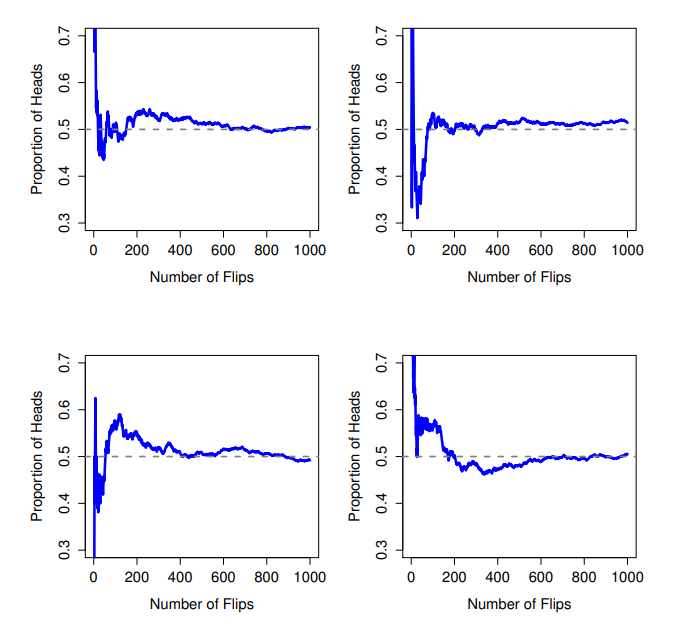
\includegraphics[width=0.9\linewidth]{images/Figure43} \caption{An illustration of how frequentist probability works. If you flip a fair coin over and over again the proportion of heads that you've seen eventually settles down and converges to the true probability of $0.5$. Each panel shows four different simulated experiments. In each case we pretend we flipped a coin $1000$ times and kept track of the proportion of flips that were heads as we went along. Although none of these sequences actually ended up with an exact value of $.5$, if we'd extended the experiment for an infinite number of coin flips they would have}\label{fig:fig7-1}
\end{figure}

\hypertarget{the-bayesian-view}{%
\subsection{The Bayesian view}\label{the-bayesian-view}}

\textbf{The Bayesian view} of probability is often called the subjectivist view, and although it has been a minority view among statisticians it has been steadily gaining traction for the last several decades. There are many flavours of Bayesianism, making it hard to say exactly what ``the'' Bayesian view is. The most common way of thinking about subjective probability is to define the probability of an event as the \textbf{degree of belief} that an intelligent and rational agent assigns to that truth of that event. From that perspective, probabilities don't exist in the world but rather in the thoughts and assumptions of people and other intelligent beings.

However, in order for this approach to work we need some way of operationalising ``degree of belief''. One way that you can do this is to formalise it in terms of ``rational gambling'', though there are many other ways. Suppose that I believe that there's a 60\% probability of rain tomorrow. If someone offers me a bet that if it rains tomorrow then I win \$5, but if it doesn't rain I lose \$5. Clearly, from my perspective, this is a pretty good bet. On the other hand, if I think that the probability of rain is only 40\% then it's a bad bet to take. So we can operationalise the notion of a ``subjective probability'' in terms of what bets I'm willing to accept.

What are the advantages and disadvantages to the Bayesian approach? The main advantage is that it allows you to assign probabilities to any event you want to. You don't need to be limited to those events that are repeatable. The main disadvantage (to many people) is that we can't be purely objective. Specifying a probability requires us to specify an entity that has the relevant degree of belief. This entity might be a human, an alien, a robot, or even a statistician. But there has to be an intelligent agent out there that believes in things. To many people this is uncomfortable, it seems to make probability arbitrary. Whilst the Bayesian approach requires that the agent in question be rational (i.e., obey the rules of probability), it does allow everyone to have their own beliefs. I can believe the coin is fair and you don't have to, even though we're both rational. The frequentist view doesn't allow any two observers to attribute different probabilities to the same event. When that happens then at least one of them must be wrong. The Bayesian view does not prevent this from occurring. Two observers with different background knowledge can legitimately hold different beliefs about the same event. In short, where the frequentist view is sometimes considered to be too narrow (forbids lots of things that that we want to assign probabilities to), the Bayesian view is sometimes thought to be too broad (allows too many differences between observers).

\hypertarget{whats-the-difference-and-who-is-right}{%
\subsection{What's the difference? And who is right?}\label{whats-the-difference-and-who-is-right}}

Now that you've seen each of these two views independently it's useful to make sure you can compare the two. Go back to the hypothetical robot soccer game at the start of the section. What do you think a frequentist and a Bayesian would say about these three statements? Which statement would a frequentist say is the correct definition of probability? Which one would a Bayesian opt for? Would some of these statements be meaningless to a frequentist or a Bayesian? If you've understood the two perspectives you should have some sense of how to answer those questions.

Okay, assuming you understand the difference then you might be wondering which of them is \emph{right}? Honestly, I don't know that there is a right answer. As far as I can tell there's nothing mathematically incorrect about the way frequentists think about sequences of events, and there's nothing mathematically incorrect about the way that Bayesians define the beliefs of a rational agent. In fact, when you dig down into the details Bayesians and frequentists actually agree about a lot of things. Many frequentist methods lead to decisions that Bayesians agree a rational agent would make. Many Bayesian methods have very good frequentist properties.

For the most part, I'm a pragmatist so I'll use any statistical method that I trust. As it turns out, that makes me prefer Bayesian methods for reasons I'll explain towards the end of the book. But I'm not fundamentally opposed to frequentist methods. Not everyone is quite so relaxed. For instance, consider Sir Ronald Fisher, one of the towering figures of 20th century statistics and a vehement opponent to all things Bayesian, whose paper on the mathematical foundations of statistics referred to Bayesian probability as ``an impenetrable jungle {[}that{]} arrests progress towards precision of statistical concepts'' (\protect\hyperlink{ref-Fisher1922b}{Fisher 1922b}) p.311. Or the psychologist Paul Meehl, who suggests that relying on frequentist methods could turn you into ``a potent but sterile intellectual rake who leaves in his merry path a long train of ravished maidens but no viable scientific offspring'' (\protect\hyperlink{ref-Meehl1967}{Meehl 1967}) p.114{]}. The history of statistics, as you might gather, is not devoid of entertainment.

In any case, whilst I personally prefer the Bayesian view, the majority of statistical analyses are based on the frequentist approach. My reasoning is pragmatic. The goal of this book is to cover roughly the same territory as a typical undergraduate stats class in psychology, and if you want to understand the statistical tools used by most psychologists you'll need a good grasp of frequentist methods. I promise you that this isn't wasted effort. Even if you end up wanting to switch to the Bayesian perspective, you really should read through at least one book on the ``orthodox'' frequentist view. Besides, I won't completely ignore the Bayesian perspective. Every now and then I'll add some commentary from a Bayesian point of view, and I'll revisit the topic in more depth in the chapter on {[}Bayesian statistics{]}.

\hypertarget{basic-probability-theory}{%
\section{Basic probability theory}\label{basic-probability-theory}}

Ideological arguments between Bayesians and frequentists notwithstanding, it turns out that people mostly agree on the rules that probabilities should obey. There are lots of different ways of arriving at these rules. The most commonly used approach is based on the work of Andrey Kolmogorov, one of the great Soviet mathematicians of the 20th century. I won't go into a lot of detail, but I'll try to give you a bit of a sense of how it works. And in order to do so I'm going to have to talk about my trousers.

\hypertarget{introducing-probability-distributions}{%
\subsection{Introducing probability distributions}\label{introducing-probability-distributions}}

One of the disturbing truths about my life is that I only own 5 pairs of trousers. Three pairs of jeans, the bottom half of a suit, and a pair of tracksuit pants. Even sadder, I've given them names: I call them \(X_1\), \(X_2\), \(X_3\), \(X_4\) and \(X_5\). I really have, that's why they call me Mister Imaginative. Now, on any given day, I pick out exactly one of pair of trousers to wear. Not even I'm so stupid as to try to wear two pairs of trousers, and thanks to years of training I never go outside without wearing trousers anymore. If I were to describe this situation using the language of probability theory, I would refer to each pair of trousers (i.e., each \(X\)) as an elementary event. The key characteristic of \textbf{elementary events} is that every time we make an observation (e.g., every time I put on a pair of trousers) then the outcome will be one and only one of these events. Like I said, these days I always wear exactly one pair of trousers so my trousers satisfy this constraint. Similarly, the set of all possible events is called a \textbf{sample space}. Granted, some people would call it a ``wardrobe'', but that's because they're refusing to think about my trousers in probabilistic terms. Sad.

Okay, now that we have a sample space (a wardrobe), which is built from lots of possible elementary events (trousers), what we want to do is assign a \textbf{probability} of one of these elementary events. For an event \(X\), the probability of that event \(P(X)\) is a number that lies between 0 and 1. The bigger the value of \(P(X)\), the more likely the event is to occur. So, for example, if \(P(X) = 0\) it means the event \(X\) is impossible (i.e., I never wear those trousers). On the other hand, if \(P(X) = 1\) it means that event \(X\) is certain to occur (i.e., I always wear those trousers). For probability values in the middle it means that I sometimes wear those trousers. For instance, if \(P(X) = 0.5\) it means that I wear those trousers half of the time.

At this point, we're almost done. The last thing we need to recognise is that ``something always happens''. Every time I put on trousers, I really do end up wearing trousers (crazy, right?). What this somewhat trite statement means, in probabilistic terms, is that the probabilities of the elementary events need to add up to 1. This is known as the \textbf{law of total probability}, not that any of us really care. More importantly, if these requirements are satisfied then what we have is a \textbf{probability distribution}. For example, Table \ref{tab:tab7-2} shows an example of a probability distribution.

 
  \providecommand{\huxb}[2]{\arrayrulecolor[RGB]{#1}\global\arrayrulewidth=#2pt}
  \providecommand{\huxvb}[2]{\color[RGB]{#1}\vrule width #2pt}
  \providecommand{\huxtpad}[1]{\rule{0pt}{#1}}
  \providecommand{\huxbpad}[1]{\rule[-#1]{0pt}{#1}}

\begin{table}[ht]
\begin{centerbox}
\begin{threeparttable}
\setlength{\tabcolsep}{0pt}
\begin{tabular}{l l l}


\hhline{>{\huxb{0, 0, 0}{0.4}}->{\huxb{0, 0, 0}{0.4}}->{\huxb{0, 0, 0}{0.4}}-}
\arrayrulecolor{black}

\multicolumn{1}{!{\huxvb{0, 0, 0}{0}}c!{\huxvb{0, 0, 0}{0}}}{\cellcolor[RGB]{242, 242, 242}\huxtpad{6pt + 1em}\centering \hspace{0pt} \textbf{Which trousers?} \hspace{6pt}\huxbpad{6pt}} &
\multicolumn{1}{c!{\huxvb{0, 0, 0}{0}}}{\cellcolor[RGB]{242, 242, 242}\huxtpad{6pt + 1em}\centering \hspace{6pt} \textbf{Label} \hspace{6pt}\huxbpad{6pt}} &
\multicolumn{1}{c!{\huxvb{0, 0, 0}{0}}}{\cellcolor[RGB]{242, 242, 242}\huxtpad{6pt + 1em}\centering \hspace{6pt} \textbf{Probability} \hspace{0pt}\huxbpad{6pt}} \tabularnewline[-0.5pt]


\hhline{>{\huxb{0, 0, 0}{0.4}}->{\huxb{0, 0, 0}{0.4}}->{\huxb{0, 0, 0}{0.4}}-}
\arrayrulecolor{black}

\multicolumn{1}{!{\huxvb{0, 0, 0}{0}}c!{\huxvb{0, 0, 0}{0}}}{\huxtpad{6pt + 1em}\centering \hspace{0pt} Blue jeans \hspace{6pt}\huxbpad{6pt}} &
\multicolumn{1}{c!{\huxvb{0, 0, 0}{0}}}{\huxtpad{6pt + 1em}\centering \hspace{6pt} $\backslash$(X\_1 $\backslash$) \hspace{6pt}\huxbpad{6pt}} &
\multicolumn{1}{c!{\huxvb{0, 0, 0}{0}}}{\huxtpad{6pt + 1em}\centering \hspace{6pt} $\backslash$(P(X\_1)=.5 $\backslash$) \hspace{0pt}\huxbpad{6pt}} \tabularnewline[-0.5pt]


\hhline{}
\arrayrulecolor{black}

\multicolumn{1}{!{\huxvb{0, 0, 0}{0}}c!{\huxvb{0, 0, 0}{0}}}{\cellcolor[RGB]{242, 242, 242}\huxtpad{6pt + 1em}\centering \hspace{0pt} Grey jeans \hspace{6pt}\huxbpad{6pt}} &
\multicolumn{1}{c!{\huxvb{0, 0, 0}{0}}}{\cellcolor[RGB]{242, 242, 242}\huxtpad{6pt + 1em}\centering \hspace{6pt} $\backslash$(X\_2 $\backslash$) \hspace{6pt}\huxbpad{6pt}} &
\multicolumn{1}{c!{\huxvb{0, 0, 0}{0}}}{\cellcolor[RGB]{242, 242, 242}\huxtpad{6pt + 1em}\centering \hspace{6pt} $\backslash$(P(X\_2)=.3 $\backslash$) \hspace{0pt}\huxbpad{6pt}} \tabularnewline[-0.5pt]


\hhline{}
\arrayrulecolor{black}

\multicolumn{1}{!{\huxvb{0, 0, 0}{0}}c!{\huxvb{0, 0, 0}{0}}}{\huxtpad{6pt + 1em}\centering \hspace{0pt} Black jeans \hspace{6pt}\huxbpad{6pt}} &
\multicolumn{1}{c!{\huxvb{0, 0, 0}{0}}}{\huxtpad{6pt + 1em}\centering \hspace{6pt} $\backslash$(X\_3 $\backslash$) \hspace{6pt}\huxbpad{6pt}} &
\multicolumn{1}{c!{\huxvb{0, 0, 0}{0}}}{\huxtpad{6pt + 1em}\centering \hspace{6pt} $\backslash$(P(X\_3)=.1 $\backslash$) \hspace{0pt}\huxbpad{6pt}} \tabularnewline[-0.5pt]


\hhline{}
\arrayrulecolor{black}

\multicolumn{1}{!{\huxvb{0, 0, 0}{0}}c!{\huxvb{0, 0, 0}{0}}}{\cellcolor[RGB]{242, 242, 242}\huxtpad{6pt + 1em}\centering \hspace{0pt} Black suit \hspace{6pt}\huxbpad{6pt}} &
\multicolumn{1}{c!{\huxvb{0, 0, 0}{0}}}{\cellcolor[RGB]{242, 242, 242}\huxtpad{6pt + 1em}\centering \hspace{6pt} $\backslash$(X\_4 $\backslash$) \hspace{6pt}\huxbpad{6pt}} &
\multicolumn{1}{c!{\huxvb{0, 0, 0}{0}}}{\cellcolor[RGB]{242, 242, 242}\huxtpad{6pt + 1em}\centering \hspace{6pt} $\backslash$(P(X\_4)=0 $\backslash$) \hspace{0pt}\huxbpad{6pt}} \tabularnewline[-0.5pt]


\hhline{}
\arrayrulecolor{black}

\multicolumn{1}{!{\huxvb{0, 0, 0}{0}}c!{\huxvb{0, 0, 0}{0}}}{\huxtpad{6pt + 1em}\centering \hspace{0pt} Blue tracksuit \hspace{6pt}\huxbpad{6pt}} &
\multicolumn{1}{c!{\huxvb{0, 0, 0}{0}}}{\huxtpad{6pt + 1em}\centering \hspace{6pt} $\backslash$(X\_5 $\backslash$) \hspace{6pt}\huxbpad{6pt}} &
\multicolumn{1}{c!{\huxvb{0, 0, 0}{0}}}{\huxtpad{6pt + 1em}\centering \hspace{6pt} $\backslash$(P(X\_5)=.1 $\backslash$) \hspace{0pt}\huxbpad{6pt}} \tabularnewline[-0.5pt]


\hhline{>{\huxb{0, 0, 0}{0.4}}->{\huxb{0, 0, 0}{0.4}}->{\huxb{0, 0, 0}{0.4}}-}
\arrayrulecolor{black}
\end{tabular}\captionsetup{justification=raggedright,singlelinecheck=off}
\caption{\label{tab:tab7-2} A probability distribution for trouser wearing}
 
\end{threeparttable}\par\end{centerbox}

\end{table}
 

Each of the events has a probability that lies between 0 and 1, and if we add up the probability of all events they sum to 1. Awesome. We can even draw a nice bar graph (see Section 5.3) to visualise this distribution, as shown in Figure \ref{fig:fig7-2}. And, at this point, we've all achieved something. You've learned what a probability distribution is, and I've finally managed to find a way to create a graph that focuses entirely on my trousers. Everyone wins! The only other thing that I need to point out is that probability theory allows you to talk about \textbf{non elementary events} as well as elementary ones. The easiest way to illustrate the concept is with an example. In the trousers example it's perfectly legitimate to refer to the probability that I wear jeans. In this scenario, the ``Dani wears jeans'' event is said to have happened as long as the elementary event that actually did occur is one of the appropriate ones. In this case ``blue jeans'', ``black jeans'' or ``grey jeans''. In mathematical terms we defined the ``jeans'' event \(E\) to correspond to the set of elementary events \((X1, X2, X3)\). If any of these elementary events occurs then \(E\) is also said to have occurred. Having decided to write down the definition of the E this way, it's pretty straightforward to state what the probability P(E) and, since the probabilities of blue, grey and black jeans respectively are \(.5\), \(.3\) and \(.1\), the probability that I wear jeans is equal to \(.9\). is: we just add everything up. In this particular case \[P(E)=P(X_1)+P(X_2)+P(X_3)\] At this point you might be thinking that this is all terribly obvious and simple and you'd be right. All we've really done is wrap some basic mathematics around a few common sense intuitions. However, from these simple beginnings it's possible to construct some extremely powerful mathematical tools. I'm definitely not going to go into the details in this book, but what I will do is list, in Table \ref{tab:tab7-3}, some of the other rules that probabilities satisfy. These rules can be derived from the simple assumptions that I've outlined above, but since we don't actually use these rules for anything in this book I won't do so here.

\begin{figure}
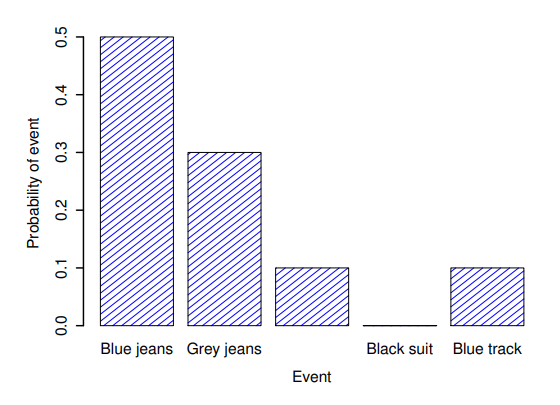
\includegraphics[width=0.9\linewidth]{images/Figure44} \caption{A visual depiction of the 'trousers' probability distribution. There are five 'elementary events', corresponding to the five pairs of trousers that I own. Each event has some probability of occurring: this probability is a number between 0 to 1. The sum of these probabilities is 1}\label{fig:fig7-2}
\end{figure}

 
  \providecommand{\huxb}[2]{\arrayrulecolor[RGB]{#1}\global\arrayrulewidth=#2pt}
  \providecommand{\huxvb}[2]{\color[RGB]{#1}\vrule width #2pt}
  \providecommand{\huxtpad}[1]{\rule{0pt}{#1}}
  \providecommand{\huxbpad}[1]{\rule[-#1]{0pt}{#1}}

\begin{table}[ht]
\begin{centerbox}
\begin{threeparttable}
\setlength{\tabcolsep}{0pt}
\begin{tabular}{l l l}


\hhline{>{\huxb{0, 0, 0}{0.4}}->{\huxb{0, 0, 0}{0.4}}->{\huxb{0, 0, 0}{0.4}}-}
\arrayrulecolor{black}

\multicolumn{1}{!{\huxvb{0, 0, 0}{0}}c!{\huxvb{0, 0, 0}{0}}}{\cellcolor[RGB]{242, 242, 242}\huxtpad{6pt + 1em}\centering \hspace{0pt} \textbf{English} \hspace{6pt}\huxbpad{6pt}} &
\multicolumn{1}{c!{\huxvb{0, 0, 0}{0}}}{\cellcolor[RGB]{242, 242, 242}\huxtpad{6pt + 1em}\centering \hspace{6pt} \textbf{Notation} \hspace{6pt}\huxbpad{6pt}} &
\multicolumn{1}{c!{\huxvb{0, 0, 0}{0}}}{\cellcolor[RGB]{242, 242, 242}\huxtpad{6pt + 1em}\centering \hspace{6pt} \textbf{Formula} \hspace{0pt}\huxbpad{6pt}} \tabularnewline[-0.5pt]


\hhline{>{\huxb{0, 0, 0}{0.4}}->{\huxb{0, 0, 0}{0.4}}->{\huxb{0, 0, 0}{0.4}}-}
\arrayrulecolor{black}

\multicolumn{1}{!{\huxvb{0, 0, 0}{0}}c!{\huxvb{0, 0, 0}{0}}}{\huxtpad{6pt + 1em}\centering \hspace{0pt} not A \hspace{6pt}\huxbpad{6pt}} &
\multicolumn{1}{c!{\huxvb{0, 0, 0}{0}}}{\huxtpad{6pt + 1em}\centering \hspace{6pt} $\backslash$(P ($\backslash$neg A) $\backslash$) \hspace{6pt}\huxbpad{6pt}} &
\multicolumn{1}{c!{\huxvb{0, 0, 0}{0}}}{\huxtpad{6pt + 1em}\centering \hspace{6pt} $\backslash$(1-P(A) $\backslash$) \hspace{0pt}\huxbpad{6pt}} \tabularnewline[-0.5pt]


\hhline{}
\arrayrulecolor{black}

\multicolumn{1}{!{\huxvb{0, 0, 0}{0}}c!{\huxvb{0, 0, 0}{0}}}{\cellcolor[RGB]{242, 242, 242}\huxtpad{6pt + 1em}\centering \hspace{0pt} A or B \hspace{6pt}\huxbpad{6pt}} &
\multicolumn{1}{c!{\huxvb{0, 0, 0}{0}}}{\cellcolor[RGB]{242, 242, 242}\huxtpad{6pt + 1em}\centering \hspace{6pt} $\backslash$(P(A $\backslash$cup B) $\backslash$) \hspace{6pt}\huxbpad{6pt}} &
\multicolumn{1}{c!{\huxvb{0, 0, 0}{0}}}{\cellcolor[RGB]{242, 242, 242}\huxtpad{6pt + 1em}\centering \hspace{6pt} $\backslash$(P(A) + P(B) - P(A $\backslash$cap B) $\backslash$) \hspace{0pt}\huxbpad{6pt}} \tabularnewline[-0.5pt]


\hhline{}
\arrayrulecolor{black}

\multicolumn{1}{!{\huxvb{0, 0, 0}{0}}c!{\huxvb{0, 0, 0}{0}}}{\huxtpad{6pt + 1em}\centering \hspace{0pt} A and B \hspace{6pt}\huxbpad{6pt}} &
\multicolumn{1}{c!{\huxvb{0, 0, 0}{0}}}{\huxtpad{6pt + 1em}\centering \hspace{6pt} $\backslash$(P(A $\backslash$cap B) $\backslash$) \hspace{6pt}\huxbpad{6pt}} &
\multicolumn{1}{c!{\huxvb{0, 0, 0}{0}}}{\huxtpad{6pt + 1em}\centering \hspace{6pt} $\backslash$(P(A$|$B) P(B) $\backslash$) \hspace{0pt}\huxbpad{6pt}} \tabularnewline[-0.5pt]


\hhline{>{\huxb{0, 0, 0}{0.4}}->{\huxb{0, 0, 0}{0.4}}->{\huxb{0, 0, 0}{0.4}}-}
\arrayrulecolor{black}
\end{tabular}\captionsetup{justification=raggedright,singlelinecheck=off}
\caption{\label{tab:tab7-3} Some rules that probabilities satisfy}
 
\end{threeparttable}\par\end{centerbox}

\end{table}
 

\hypertarget{the-binomial-distribution}{%
\section{The binomial distribution}\label{the-binomial-distribution}}

As you might imagine, probability distributions vary enormously and there's an enormous range of distributions out there. However, they aren't all equally important. In fact, the vast majority of the content in this book relies on one of five distributions: the binomial distribution, the normal distribution, the t distribution, the \(\chi^2\) (``chi-square'') distribution and the F distribution. Given this, what I'll do over the next few sections is provide a brief introduction to all five of these, paying special attention to the binomial and the normal. I'll start with the binomial distribution since it's the simplest of the five.

\hypertarget{introducing-the-binomial}{%
\subsection{Introducing the binomial}\label{introducing-the-binomial}}

The theory of probability originated in the attempt to describe how games of chance work, so it seems fitting that our discussion of the \textbf{binomial distribution} should involve a discussion of rolling dice and flipping coins. Let's imagine a simple ``experiment''. In my hot little hand I'm holding 20 identical six-sided dice. On one face of each die there's a picture of a skull, the other five faces are all blank. If I proceed to roll all 20 dice, what's the probability that I'll get exactly 4 skulls? Assuming that the dice are fair, we know that the chance of any one die coming up skulls is 1 in 6. To say this another way, the skull probability for a single die is approximately .167. This is enough information to answer our question, so let's have a look at how it's done.

As usual, we'll want to introduce some names and some notation. We'll let \(N\) denote the number of dice rolls in our experiment, which is often referred to as the \textbf{size parameter} of our binomial distribution. We'll also use \(\theta\) to refer to the the probability that a single die comes up skulls, a quantity that is usually called the \textbf{success probability} of the binomial.\footnote{Note that the term ``success'' is pretty arbitrary and doesn't actually imply that the outcome is something to be desired. If \(\theta\) referred to the probability that any one passenger gets injured in a bus crash I'd still call it the success probability, but that doesn't mean I want people to get hurt in bus crashes!} Finally, we'll use \(X\) to refer to the results of our experiment, namely the number of skulls I get when I roll the dice. Since the actual value of \(X\) is due to chance we refer to it as a \textbf{random variable}. In any case, now that we have all this terminology and notation we can use it to state the problem a little more precisely. The quantity that we want to calculate is the probability that \(X = 4\) given that we know that \(\theta = .167\) and \(N = 20\). The general ``form'' of the thing I'm interested in calculating could be written as

\[P(X|\theta,N)\]

and we're interested in the special case where \$X = 4, \theta = .167 \$ and \(N = 20\).

Statistical notation \footnote{For those readers who know a little calculus, I'll give a slightly more precise explanation. In the same way that probabilities are non-negative numbers that must sum to 1, probability densities are non-negative numbers that must integrate to 1 (where the integral is taken across all possible values of X). To calculate the probability that X falls between a and b we calculate the definite integral of the density function over the corresponding range, \(\int\_{a}^{b} p(x) dx\). If you don't remember or never learned calculus, don't worry about this. It's not needed for this book.}

Yeah, yeah. I know what you're thinking: notation, notation, notation. Really, who cares? Very few readers of this book are here for the notation, so I should probably move on and talk about how to use the binomial distribution. I've included the formula for the binomial distribution in Table \ref{tab:tab7-2}, since some readers may want to play with it themselves, but since most people probably don't care that much and because we don't need the formula in this book, I won't talk about it in any detail. Instead, I just want to show you what the binomial distribution looks like.

To that end, Figure \ref{fig:fig7-3} plots the binomial probabilities for all possible values of \(X\) for our dice rolling experiment, from \(X = 0\) (no skulls) all the way up to \(X = 20\) (all skulls). Note that this is basically a bar chart, and is no different to the ``trousers probability'' plot I drew in Figure \ref{fig:fig7-2}. On the horizontal axis we have all the possible events, and on the vertical axis we can read off the probability of each of those events. So, the probability of rolling \(4\) skulls out of \(20\) is about \(0.20\) (the actual answer is \(0.2022036\), as we'll see in a moment). In other words, you'd expect that to happen about 20\% of the times you repeated this experiment.

To give you a feel for how the binomial distribution changes when we alter the values of \(theta\) and \(N\), let's suppose that instead of rolling dice I'm actually flipping coins. This time around, my experiment involves flipping a fair coin repeatedly and the outcome that I'm interested in is the number of heads that I observe. In this scenario, the success probability is now \(\theta = \frac{1}{2}\). Suppose I were to flip the coin \(N = 20\) times. In this example, I've changed the success probability but kept the size of the experiment the same. What does this do to our binomial distribution? Well, as Figure \ref{fig:fig7-4} shows, the main effect of this is to shift the whole distribution, as you'd expect. Okay, what if we flipped a coin \(N = 100\) times? Well, in that case we get Figure \textbf{7.4b}. The distribution stays roughly in the middle but there's a bit more variability in the possible outcomes.

\begin{figure}
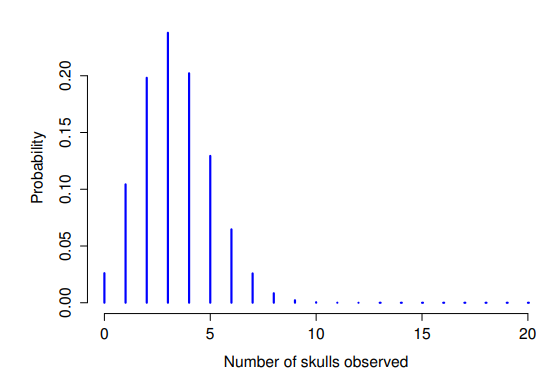
\includegraphics[width=0.9\linewidth]{images/Figure45} \caption{The binomial distribution with size parameter of $N = 20$ and an underlying success probability of $\theta = \frac{1}{6}$. Each vertical bar depicts the probability of one specific outcome (i.e., one possible value of X). Because this is a probability distribution, each of the probabilities must be a number between 0 and 1, and the heights of the bars must sum to 1 as well}\label{fig:fig7-3}
\end{figure}

I were to flip the coin \(N = 20\) times. In this example, I've changed the success probability but kept the size of the experiment the same. What does this do to our binomial distribution? Well, as Figure \textbf{7.4a} shows, the main effect of this is to shift the whole distribution, as you'd expect. Okay, what if we flipped a coin \(N = 100\) times? Well, in that case we get Figure \textbf{7.4b}. The distribution stays roughly in the middle but there's a bit more variability in the possible outcomes.

\hypertarget{the-normal-distribution}{%
\section{The normal distribution}\label{the-normal-distribution}}

While the binomial distribution is conceptually the simplest distribution to understand, it's not the most important one. That particular honour goes to the normal distribution, also referred to as ``the bell curve'' or a ``Gaussian distribution''. A \textbf{normal distribution} is described using two parameters: the mean of the distribution µ and the standard deviation of the distribution \(\sigma\).

\begin{figure}
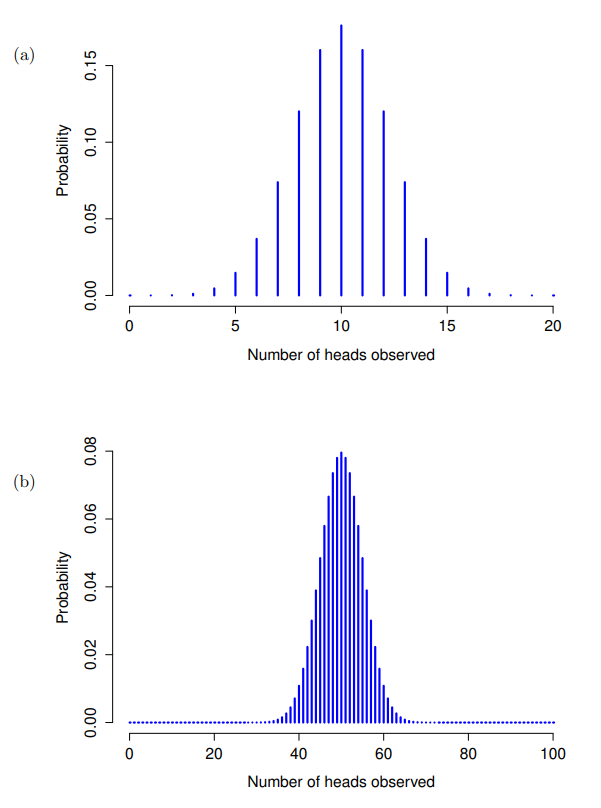
\includegraphics[width=0.9\linewidth]{images/Figure46} \caption{Two binomial distributions, involving a scenario in which I'm flipping a fair coin, so the underlying success probability is $  heta = rac{1}{2}$. In panel (a), we assume I'm flipping the coin $N = 20$ times. In panel (b) we assume that the coin is flipped $N = 100$ times}\label{fig:fig7-4}
\end{figure}

\begin{figure}
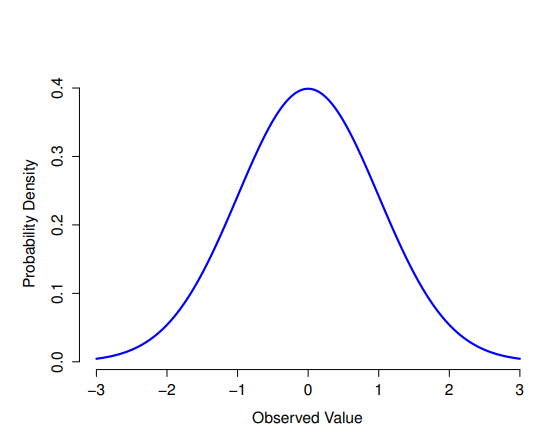
\includegraphics[width=0.9\linewidth]{images/Figure47} \caption{The normal distribution with mean $\mu = 0$ and standard deviation $\sigma = 1$. The x-axis corresponds to the value of some variable, and the y-axis tells us something about how likely we are to observe that value. However, notice that the y-axis is labelled *Probability Density* and not *Probability*. There is a subtle and somewhat frustrating characteristic of continuous distributions that makes the $y$ axis behave a bit oddly: the height of the curve here isn't actually the probability of observing a particular x value. On the other hand, it is true that the heights of the curve tells you which $x$ values are more likely (the higher ones!). (see Section 7.5.1 for all the annoying details)}\label{fig:fig7-5}
\end{figure}

Statistical notation \footnote{The notation that we sometimes use to say that a variable \(X\) is normally distributed is as follows: \[X \sim Normal(\mu,\sigma) \] Of course, that's just notation. It doesn't tell us anything interesting about the normal distribution itself. As was the case with the binomial distribution, I have included the formula for the normal distribution in this book, because I think it's important enough that everyone who learns statistics should at least look at it, but since this is an introductory text I don't want to focus on it, so I've tucked it away in this footnote.}

Let's try to get a sense for what it means for a variable to be normally distributed. To that end, have a look at Figure \ref{fig:fig7-5} which plots a normal distribution with mean \(\mu = 0\) and standard deviation \(\sigma = 1\). You can see where the name ``bell curve'' comes from; it looks a bit like a bell. Notice that, unlike the plots that I drew to illustrate the binomial distribution, the picture of the normal distribution in Figure \ref{fig:fig7-5} shows a smooth curve instead of ``histogram-like'' bars. This isn't an arbitrary choice, the normal distribution is continuous whereas the binomial is discrete. For instance, in the die rolling example from the last section it was possible to get 3 skulls or 4 skulls, but impossible to get 3.9 skulls. The figures that I drew in the previous section reflected this fact. In Figure \ref{fig:fig7-3}, for instance, there's a bar located at \(X = 3\) and another one at \(X = 4\) but there's nothing in between. Continuous quantities don't have this constraint. For instance, suppose we're talking about the weather. The temperature on a pleasant Spring day could be 23 degrees, 24 degrees, 23.9 degrees, or anything in between since temperature is a continuous variable. And so a normal distribution might be quite appropriate for describing Spring temperatures\footnote{In practice, the normal distribution is so handy that people tend to use it even when the variable isn't actually continuous. As long as there are enough categories (e.g., Likert scale responses to a questionnaire), it's pretty standard practice to use the normal distribution as an approximation. This works out much better in practice than you'd think.}

\begin{figure}
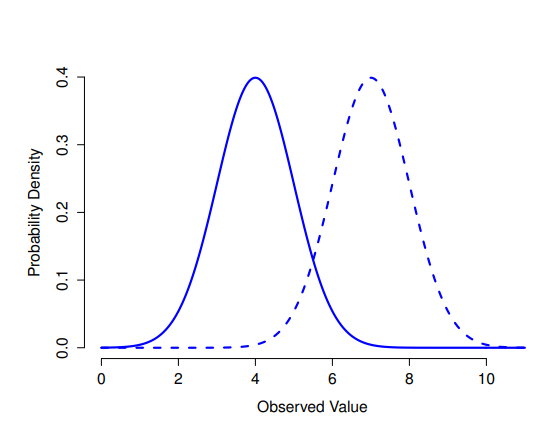
\includegraphics[width=0.9\linewidth]{images/Figure48} \caption{An illustration of what happens when you change the mean of a normal distribution. The solid line depicts a normal distribution with a mean of $\mu = 4$. The dashed line shows a normal distribution with a mean of $mu = 7$. In both cases, the standard deviation is $\sigma = 1$. Not surprisingly, the two distributions have the same shape, but the dashed line is shifted to the right}\label{fig:fig7-6}
\end{figure}

With this in mind, let's see if we can't get an intuition for how the normal distribution works. First, let's have a look at what happens when we play around with the parameters of the distribution. To that end, Figure \ref{fig:fig7-6} plots normal distributions that have different means but have the same standard deviation. As you might expect, all of these distributions have the same ``width''. The only difference between them is that they've been shifted to the left or to the right. In every other respect they're identical. In contrast, if we increase the standard deviation while keeping the mean constant, the peak of the distribution stays in the same place but the distribution gets wider, as you can see in Figure \ref{fig:fig7-7}. Notice, though, that when we widen the distribution the height of the peak shrinks. This has to happen, in the same way that the heights of the bars that we used to draw a discrete binomial distribution have to sum to 1, the total area under the curve for the normal distribution must equal 1. Before moving on, I want to point out one important characteristic of the normal distribution. Irrespective of what the actual mean and standard deviation are, 68.3\% of the area falls within 1 standard deviation of the mean. Similarly, \(95.4\\%\) of the distribution falls within 2 standard deviations of the mean, and \((99.7\\%\) of the distribution is within 3 standard deviations. This idea is illustrated in Figure \ref{fig:fig7-8}; see also Figure \ref{fig:fig7-9}.

\begin{figure}
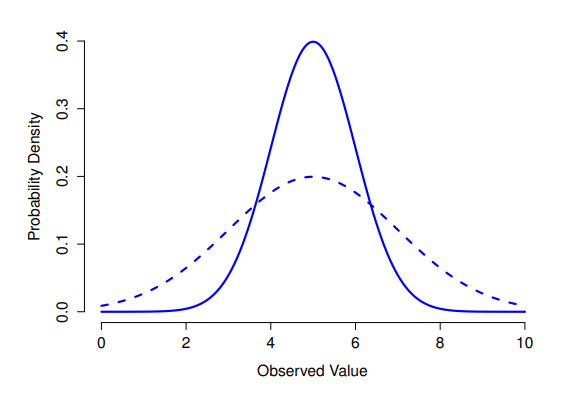
\includegraphics[width=0.9\linewidth]{images/Figure49} \caption{An illustration of what happens when you change the the standard deviation of a normal distribution. Both distributions plotted in this figure have a mean of $\mu = 5$, but they have different standard deviations. The solid line plots a distribution with standard deviation $\sigma = 1$, and the dashed line shows a distribution with standard deviation $\sigma = 2$. As a consequence, both distributions are 'centred' on the same spot, but the dashed line is wider than the solid one}\label{fig:fig7-7}
\end{figure}

\textbackslash begin\{figure\}
\includegraphics[width=0.9\linewidth]{images/Figure50} \textbackslash caption\{The area under the curve tells you the probability that an observation falls within a particular range. The solid lines plot normal distributions with mean \(\mu = 0\) and standard deviation \(\sigma = 1\). The shaded areas illustrate `areas under the curve' for two important cases. In panel a, we can see that there is a 68.3\% chance that an observation will fall within one standard deviation of the mean. In panel b, we see that there is a 95.4\% chance that an observation will fall within two standard deviations of the mean\}\label{fig:fig7-8}
\textbackslash end\{figure\}

\textbackslash begin\{figure\}
\includegraphics[width=0.9\linewidth]{images/Figure51} \textbackslash caption\{Two more examples of the `area under the curve idea'. There is a 15.9\% chance that an observation is one standard deviation below the mean or smaller (panel a), and a 34.1\% chance that the observation is somewhere between one standard deviation below the mean and the mean (panel b). Notice that if you add these two numbers together you get 15.9\% + 34.1\% = 50\%. For normally distributed data, there is a 50\% chance that an observation falls below the mean. And of course that also implies that there is a 50\% chance that it falls above the mean\}\label{fig:fig7-9}
\textbackslash end\{figure\}

\hypertarget{probability-density}{%
\subsection{Probability density}\label{probability-density}}

There's something I've been trying to hide throughout my discussion of the normal distribution, something that some introductory textbooks omit completely. They might be right to do so. This ``thing'' that I'm hiding is weird and counter-intuitive even by the admittedly distorted standards that apply in statistics. Fortunately, it's not something that you need to understand at a deep level in order to do basic statistics. Rather, it's something that starts to become important later on when you move beyond the basics. So, if it doesn't make complete sense, don't worry too much, but try to make sure that you follow the gist of it.

Throughout my discussion of the normal distribution there's been one or two things that don't quite make sense. Perhaps you noticed that the y-axis in these figures is labelled ``Probability Density'' rather than density. Maybe you noticed that I used \(P(X)\) instead of \(P(X)\) when giving the formula for the normal distribution.

As it turns out, what is presented here isn't actually a probability, it's something else. To understand what that something is you have to spend a little time thinking about what it really means to say that \(X\) is a continuous variable. Let's say we're talking about the temperature outside. The thermometer tells me it's \(23\) degrees, but I know that's not really true. It's not exactly \(23\) degrees. Maybe it's \(23.1\) degrees, I think to myself. But I know that that's not really true either because it might actually be \(23.09\) degrees. But I know that\ldots{} well, you get the idea. The tricky thing with genuinely continuous quantities is that you never really know exactly what they are.

Now think about what this implies when we talk about probabilities. Suppose that tomorrow's maximum temperature is sampled from a normal distribution with mean \(23\) and standard deviation 1. What's the probability that the temperature will be exactly \(23\) degrees? The answer is ``zero'', or possibly ``a number so close to zero that it might as well be zero''. Why is this? It's like trying to throw a dart at an infinitely small dart board. No matter how good your aim, you'll never hit it. In real life you'll never get a value of exactly \(23\). It'll always be something like \(23.1\) or \(22.99998\) or suchlike. In other words, it's completely meaningless to talk about the probability that the temperature is exactly \(23\) degrees. However, in everyday language if I told you that it was \(23\) degrees outside and it turned out to be \(22.9998\) degrees you probably wouldn't call me a liar. Because in everyday language ``\(23\) degrees'' usually means something like ``somewhere between \(22.5\) and \(23.5\) degrees''. And while it doesn't feel very meaningful to ask about the probability that the temperature is exactly \(23\) degrees, it does seem sensible to ask about the probability that the temperature lies between \(22.5\) and \(23.5\), or between \(20\) and \(30\), or any other range of temperatures.

The point of this discussion is to make clear that when we're talking about continuous distributions it's not meaningful to talk about the probability of a specific value. However, what we can talk about is the probability that the value lies within a particular range of values. To find out the probability associated with a particular range what you need to do is calculate the ``area under the curve''. We've seen this concept already, in Figure \ref{fig:fig7-8} the shaded areas shown depict genuine probabilities (e.g., in Figure \ref{fig:fig7-8} it shows the probability of observing a value that falls within 1 standard deviation of the mean).

Okay, so that explains part of the story. I've explained a little bit about how continuous probability distributions should be interpreted (i.e., area under the curve is the key thing). But what does the formula for ppxq that I described earlier actually mean? Obviously, \(P(x)\) doesn't describe a probability, but what is it? The name for this quantity \(P(x)\) is a \textbf{probability density}, and in terms of the plots we've been drawing it corresponds to the height of the curve. The densities themselves aren't meaningful in and of themselves, but they're ``rigged'' to ensure that the area under the curve is always interpretable as genuine probabilities. To be honest, that's about as much as you really need to know for now.\footnote{For those readers who know a little calculus, I'll give a slightly more precise explanation. In the same way that probabilities are non-negative numbers that must sum to 1, probability densities are non-negative numbers that must integrate to 1 (where the integral is taken across all possible values of X). To calculate the probability that X falls between a and b we calculate the definite integral of the density function over the corresponding range, \(\int\_{a}^{b} p(x) dx\). If you don't remember or never learned calculus, don't worry about this. It's not needed for this book.}

\hypertarget{other-useful-distributions}{%
\section{Other useful distributions}\label{other-useful-distributions}}

The normal distribution is the distribution that statistics makes most use of (for reasons to be discussed shortly), and the binomial distribution is a very useful one for lots of purposes. But the world of statistics is filled with probability distributions, some of which we'll run into in passing. In particular, the three that will appear in this book are the t distribution, the \(\chi^2\) distribution and the F distribution. I won't give formulas for any of these, or talk about them in too much detail, but I will show you some pictures: Figures @ref(fig:fig7-10, \ref{fig:fig7-1} and \ref{fig:fig7-12}).

\begin{figure}
\includegraphics[width=0.9\linewidth]{images/Figure52} \caption{A $t$ distribution with 3 degrees of freedom (solid line). It looks similar to a normal distribution, but it's not quite the same. For comparison purposes I've plotted a standard normal distribution as the dashed line}\label{fig:fig7-10}
\end{figure}

\begin{figure}
\includegraphics[width=0.9\linewidth]{images/Figure53} \caption{$\chi^2$ distribution with 3 degrees of freedom. Notice that the observed values must always be greater than zero, and that the distribution is pretty skewed. These are the key features of a chi-square  distribution}\label{fig:fig7-11}
\end{figure}

\begin{figure}
\includegraphics[width=0.9\linewidth]{images/Figure54} \caption{An $F$ distribution with 3 and 5 degrees of freedom. Qualitatively speaking, it looks pretty similar to a chi-square distribution, but they're not quite the same in general}\label{fig:fig7-12}
\end{figure}

\begin{itemize}
\tightlist
\item
  The \(t\) distribution is a continuous distribution that looks very similar to a normal distribution, see Figure \ref{fig:fig7-10}. Note that the ``tails'' of the t distribution are ``heavier'' (i.e., extend further outwards) than the tails of the normal distribution). That's the important difference between the two. This distribution tends to arise in situations where you think that the data actually follow a normal distribution, but you don't know the mean or standard deviation. We'll run into this distribution again in the chapter on \protect\hyperlink{comparing-two-means}{Comparing two means}.
\item
  The \(\chi^2\) distribution is another distribution that turns up in lots of different places. The situation in which we'll see it is when doing \protect\hyperlink{categorical-data-analysis}{Categorical data analysis}, but it's one of those things that actually pops up all over the place. When you dig into the maths (and who doesn't love doing that?), it turns out that the main reason why the \(\chi^2\) distribution turns up all over the place is that if you have a bunch of variables that are normally distributed, square their values and then add them up (a procedure referred to as taking a ``sum of squares''), this sum has a \(\chi^2\) distribution. You'd be amazed how often this fact turns out to be useful. Anyway, here's what a \(\chi^2\) distribution looks like: Figure \ref{fig:fig7-11}.
\item
  The \(F\) distribution looks a bit like a \(\chi^2\) distribution, and it arises whenever you need to compare two \(\chi^2\) distributions to one another. Admittedly, this doesn't exactly sound like something that any sane person would want to do, but it turns out to be very important in real world data analysis. Remember when I said that \(\chi^2\) turns out to be the key distribution when we're taking a ``sum of squares''? Well, what that means is if you want to compare two different ``sums of squares'', you're probably talking about something that has an F distribution. Of course, as yet I still haven't given you an example of anything that involves a sum of squares, but I will in the Chapter on {[}Comparing several means (one-way ANOVA){]}. And that's where we'll run into the F distribution. Oh, and there's a picture in Figure \ref{fig:fig7-12}.
\end{itemize}

Okay, time to wrap this section up. We've seen three new distributions: \(\chi^2\)), \(t\) and \(F\). They're all continuous distributions, and they're all closely related to the normal distribution. The main thing for our purposes is that you grasp the basic idea that these distributions are all deeply related to one another, and to the normal distribution. Later on in this book we're going to run into data that are normally distributed, or at least assumed to be normally distributed. What I want you to understand right now is that, if you make the assumption that your data are normally distributed, you shouldn't be surprised to see \(\chi^2\), \(t\) and \(F\) distributions popping up all over the place when you start trying to do your data analysis.

\hypertarget{summary-5}{%
\section{Summary}\label{summary-5}}

In this chapter we've talked about probability. We've talked about what probability means and why statisticians can't agree on what it means. We talked about the rules that probabilities have to obey. And we introduced the idea of a probability distribution and spent a good chunk of the chapter talking about some of the more important probability distributions that statisticians work with. The section by section breakdown looks like this:

\begin{itemize}
\tightlist
\item
  Probability theory versus statistics: \protect\hyperlink{how-are-probability-and-statistics-different}{How are probability and statistics different?}
\item
  \protect\hyperlink{the-frequentist-view}{The frequentist view} versus \protect\hyperlink{the-bayesian-view}{The Bayesian view} of probability
\item
  \protect\hyperlink{basic-probability-theory}{Basic probability theory}
\item
  \protect\hyperlink{the-binomial-distribution}{The binomial distribution}, \protect\hyperlink{the-normal-distribution}{The normal distribution}, and {[}Other distributions{]}
\end{itemize}

As you'd expect, my coverage is by no means exhaustive. Probability theory is a large branch of mathematics in its own right, entirely separate from its application to statistics and data analysis. As such, there are thousands of books written on the subject and universities generally offer multiple classes devoted entirely to probability theory. Even the ``simpler'' task of documenting standard probability distributions is a big topic. I've described five standard probability distributions in this chapter, but sitting on my bookshelf I have a 45-chapter book called ``Statistical Distributions'' (\protect\hyperlink{ref-Evans2011}{M. Evans, Hastings, and Peacock 2011}) that lists a lot more than that. Fortunately for you, very little of this is necessary. You're unlikely to need to know dozens of statistical distributions when you go out and do real world data analysis, and you definitely won't need them for this book, but it never hurts to know that there's other possibilities out there.

Picking up on that last point, there's a sense in which this whole chapter is something of a digression. Many undergraduate psychology classes on statistics skim over this content very quickly (I know mine did), and even the more advanced classes will often ``forget'' to revisit the basic foundations of the field. Most academic psychologists would not know the difference between probability and density, and until recently very few would have been aware of the difference between Bayesian and frequentist probability. However, I think it's important to understand these things before moving onto the applications. For example, there are a lot of rules about what you're ``allowed'' to say when doing statistical inference and many of these can seem arbitrary and weird. However, they start to make sense if you understand that there is this Bayesian vs.~frequentist distinction. Similarly, in the chapter on \protect\hyperlink{comparing-two-means}{Comparing two means} we're going to talk about something called the t-test, and if you really want to have a grasp of the mechanics of the t-test it really helps to have a sense of what a t-distribution actually looks like. You get the idea, I hope.

\hypertarget{estimating-unkown-quantities-from-a-sample}{%
\chapter{Estimating unkown quantities from a sample}\label{estimating-unkown-quantities-from-a-sample}}

At the start of the last chapter I highlighted the critical distinction between descriptive statistics and \emph{inferential statistics}. As discussed in the chapter on \protect\hyperlink{descriptive-statistics}{Descriptive statistics}, the role of descriptive statistics is to concisely summarise what we \emph{do} know. In contrast, the purpose of inferential statistics is to ``learn what we do not know from what we do''. Now that we have a foundation in probability theory we are in a good position to think about the problem of statistical inference. What kinds of things would we like to learn about? And how do we learn them? These are the questions that lie at the heart of inferential statistics, and they are traditionally divided into two ``big ideas'': estimation and hypothesis testing. The goal in this chapter is to introduce the first of these big ideas, estimation theory, but I'm going to witter on about sampling theory first because estimation theory doesn't make sense until you understand sampling. As a consequence, this chapter divides naturally into two parts, the first three sections are focused on sampling theory, and the last two sections make use of sampling theory to discuss how statisticians think about estimation.

\hypertarget{samples-populations-and-sampling}{%
\section{Samples, populations and sampling}\label{samples-populations-and-sampling}}

In the \protect\hyperlink{prelude-to-part-iv}{Prelude to Part IV} I discussed the riddle of induction and highlighted the fact that all learning requires you to make assumptions. Accepting that this is true, our first task to come up with some fairly general assumptions about data that make sense. This is where \textbf{sampling theory} comes in. If probability theory is the foundations upon which all statistical theory builds, sampling theory is the frame around which you can build the rest of the house. Sampling theory plays a huge role in specifying the assumptions upon which your statistical inferences rely. And in order to talk about ``making inferences'' the way statisticians think about it we need to be a bit more explicit about what it is that we're drawing inferences \emph{from} (the sample) and what it is that we're drawing inferences about (the population).

In almost every situation of interest what we have available to us as researchers is a \textbf{sample} of data. We might have run experiment with some number of participants, a polling company might have phoned some number of people to ask questions about voting intentions, and so on. In this way the data set available to us is finite and incomplete. We can't possibly get every person in the world to do our experiment, for example a polling company doesn't have the time or the money to ring up every voter in the country. In our earlier discussion of \protect\hyperlink{descriptive-statistics}{Descriptive statistics} this sample was the only thing we were interested in. Our only goal was to find ways of describing, summarising and graphing that sample. This is about to change.

\hypertarget{defining-a-population}{%
\subsection{Defining a population}\label{defining-a-population}}

A sample is a concrete thing. You can open up a data file and there's the data from your sample. A \textbf{population}, on the other hand, is a more abstract idea. It refers to the set of all possible people, or all possible observations, that you want to draw conclusions about and is generally \emph{much bigger} than the sample. In an ideal world the researcher would begin the study with a clear idea of what the population of interest is, since the process of designing a study and testing hypotheses with the data does depend on the population about which you want to make statements.

Sometimes it's easy to state the population of interest. For instance, in the ``polling company'' example that opened the chapter the population consisted of all voters enrolled at the time of the study, millions of people. The sample was a set of 1000 people who all belong to that population. In most studies the situation is much less straightforward. In a typical psychological experiment determining the population of interest is a bit more complicated. Suppose I run an experiment using 100 undergraduate students as my participants. My goal, as a cognitive scientist, is to try to learn something about how the mind works. So, which of the following would count as ``the population'':

\begin{itemize}
\tightlist
\item
  All of the undergraduate psychology students at the University of Adelaide?
\item
  Undergraduate psychology students in general, anywhere in the world?
\item
  Australians currently living?
\item
  Australians of similar ages to my sample?
\item
  Anyone currently alive?
\item
  Any human being, past, present or future?
\item
  Any biological organism with a sufficient degree of intelligence operating in a terrestrial environment?
\item
  Any intelligent being?
\end{itemize}

Each of these defines a real group of mind-possessing entities, all of which might be of interest to me as a cognitive scientist, and it's not at all clear which one ought to be the true population of interest. As another example, consider the Wellesley-Croker game that we discussed in the \protect\hyperlink{prelude-to-part-iv}{Prelude to Part IV}. The sample here is a specific sequence of 12 wins and 0 losses for Wellesley. What is the population? Again, it's not obvious what the population is.

\begin{itemize}
\tightlist
\item
  All outcomes until Wellesley and Croker arrived at their destination?
\item
  All outcomes if Wellesley and Croker had played the game for the rest of their lives?
\item
  All outcomes if Wellseley and Croker lived forever and played the game until the world ran out of hills?
\item
  All outcomes if we created an infinite set of parallel universes and the Wellesely/Croker pair made guesses about the same 12 hills in each universe?
\end{itemize}

\begin{figure}
\includegraphics[width=0.9\linewidth]{images/Figure55} \caption{Simple random sampling without replacement from a finite population}\label{fig:fig8-1}
\end{figure}

\hypertarget{simple-random-samples}{%
\subsection{Simple random samples}\label{simple-random-samples}}

Irrespective of how I define the population, the critical point is that the sample is a subset of the population and our goal is to use our knowledge of the sample to draw inferences about the properties of the population. The relationship between the two depends on the procedure by which the sample was selected. This procedure is referred to as a \textbf{sampling method} and it is important to understand why it matters.

To keep things simple, let's imagine that we have a bag containing 10 chips. Each chip has a unique letter printed on it so we can distinguish between the 10 chips. The chips come in two colours, black and white. This set of chips is the population of interest and it is depicted graphically on the left of Figure \ref{fig:fig8-1}. As you can see from looking at the picture there are 4 black chips and 6 white chips, but of course in real life we wouldn't know that unless we looked in the bag. Now imagine you run the following ``experiment'': you shake up the bag, close your eyes, and pull out 4 chips without putting any of them back into the bag. First out comes the a chip (black), then the c chip (white), then j (white) and then finally b (black). If you wanted you could then put all the chips back in the bag and repeat the experiment, as depicted on the right hand side of Figure \ref{fig:fig8-1}. Each time you get different results but the procedure is identical in each case. The fact that the same procedure can lead to different results each time we refer to as a \emph{random process}.\footnote{The proper mathematical definition of randomness is extraordinarily technical, and way beyond the scope of this book. We'll be non-technical here and say that a process has an element of randomness to it whenever it is possible to repeat the process and get different answers each time.} However, because we shook the bag before pulling any chips out, it seems reasonable to think that every chip has the same chance of being selected. A procedure in which every member of the population has the same chance of being selected is called a \textbf{simple random sample}. The fact that we did not put the chips back in the bag after pulling them out means that you can't observe the same thing twice, and in such cases the observations are said to have been sampled \textbf{without replacement}.

\begin{figure}
\includegraphics[width=0.9\linewidth]{images/Figure56} \caption{Biased sampling without replacement from a finite population}\label{fig:fig8-2}
\end{figure}

\begin{figure}
\includegraphics[width=0.9\linewidth]{images/Figure57} \caption{Simple random sampling *with* replacement from a finite population}\label{fig:fig8-3}
\end{figure}

To help make sure you understand the importance of the sampling procedure, consider an alternative way in which the experiment could have been run. Suppose that my 5-year old son had opened the bag and decided to pull out four black chips without putting any of them back in the bag. This biased sampling scheme is depicted in Figure \ref{fig:fig8-2}. Now consider the evidential value of seeing 4 black chips and 0 white chips. Clearly it depends on the sampling scheme, does it not? If you know that the sampling scheme is biased to select only black chips then a sample that consists of only black chips doesn't tell you very much about the population! For this reason statisticians really like it when a data set can be considered a simple random sample, because it makes the data analysis \emph{much} easier.

A third procedure is worth mentioning. This time around we close our eyes, shake the bag, and pull out a chip. This time, however, we record the observation and then put the chip back in the bag. Again we close our eyes, shake the bag, and pull out a chip. We then repeat this procedure until we have 4 chips. Data sets generated in this way are still simple random samples, but because we put the chips back in the bag immediately after drawing them it is referred to as a sample \textbf{with replacement}. The difference between this situation and the first one is that it is possible to observe the same population member multiple times, as illustrated in Figure \ref{fig:fig8-3}.

In my experience, most psychology experiments tend to be sampling without replacement, because the same person is not allowed to participate in the experiment twice. However, most statistical theory is based on the assumption that the data arise from a simple random sample \textbf{with replacement}. In real life this very rarely matters. If the population of interest is large (e.g., has more than 10 entities!) the difference between sampling with- and without- replacement is too small to be concerned with. The difference between simple random samples and biased samples, on the other hand, is not such an easy thing to dismiss.

\hypertarget{most-samples-are-not-simple-random-samples}{%
\subsection{Most samples are not simple random samples}\label{most-samples-are-not-simple-random-samples}}

As you can see from looking at the list of possible populations that I showed above, it is almost impossible to obtain a simple random sample from most populations of interest. When I run experiments I'd consider it a minor miracle if my participants turned out to be a random sampling of the undergraduate psychology students at Adelaide university, even though this is by far the narrowest population that I might want to generalise to. A thorough discussion of other types of sampling schemes is beyond the scope of this book, but to give you a sense of what's out there I'll list a few of the more important ones.

\begin{itemize}
\tightlist
\item
  \emph{Stratified sampling}. Suppose your population is (or can be) divided into several different sub-populations, or strata. Perhaps you're running a study at several different sites, for example. Instead of trying to sample randomly from the population as a whole, you instead try to collect a separate random sample from each of the strata. Stratified sampling is sometimes easier to do than simple random sampling, especially when the population is already divided into the distinct strata. It can also be more efficient than simple random sampling, especially when some of the sub-populations are rare. For instance, when studying schizophrenia it would be much better to divide the population into two \footnote{Nothing in life is that simple. There's not an obvious division of people into binary categories like ``schizophrenic'' and ``not schizophrenic''. But this isn't a clinical psychology text so please forgive me a few simplifications here and there.} strata (schizophrenic and not-schizophrenic) and then sample an equal number of people from each group. If you selected people randomly you would get so few schizophrenic people in the sample that your study would be useless. This specific kind of of stratified sampling is referred to as oversampling because it makes a deliberate attempt to over-represent rare groups
\item
  \emph{Snowball sampling} is a technique that is especially useful when sampling from a ``hidden'' or hard to access population and is especially common in social sciences. For instance, suppose the researchers want to conduct an opinion poll among transgender people. The research team might only have contact details for a few trans folks, so the survey starts by asking them to participate (stage 1). At the end of the survey the participants are asked to provide contact details for other people who might want to participate. In stage 2 those new contacts are surveyed. The process continues until the researchers have sufficient data. The big advantage to snowball sampling is that it gets you data in situations that might otherwise be impossible to get any. On the statistical side, the main disadvantage is that the sample is highly non-random, and non-random in ways that are difficult to address. On the real life side, the disadvantage is that the procedure can be unethical if not handled well, because hidden populations are often hidden for a reason. I chose transgender people as an example here to highlight this issue. If you weren't careful you might end up outing people who don't want to be outed (very, very bad form), and even if you don't make that mistake it can still be intrusive to use people's social networks to study them. It's certainly very hard to get people's informed consent before contacting them, yet in many cases the simple act of contacting them and saying ``hey we want to study you'' can be hurtful. Social networks are complex things, and just because you can use them to get data doesn't always mean you should.
\item
  \emph{Convenience sampling} is more or less what it sounds like. The samples are chosen in a way that is convenient to the researcher, and not selected at random from the population of interest. Snowball sampling is one type of convenience sampling, but there are many others. A common example in psychology are studies that rely on undergraduate psychology students. These samples are generally non-random in two respects. First, reliance on undergraduate psychology students automatically means that your data are restricted to a single sub-population. Second, the students usually get to pick which studies they participate in, so the sample is a self selected subset of psychology students and not a randomly selected subset. In real life most studies are convenience samples of one form or another. This is sometimes a severe limitation, but not always.
\end{itemize}

\hypertarget{how-much-does-it-matter-if-you-dont-have-a-simple-random-sample}{%
\subsection{How much does it matter if you don't have a simple random sample?}\label{how-much-does-it-matter-if-you-dont-have-a-simple-random-sample}}

Okay, so real world data collection tends not to involve nice simple random samples. Does that matter? A little thought should make it clear to you that it can matter if your data are not a simple random sample. Just think about the difference between Figures \ref{fig:fig8-1} and \ref{fig:fig8-2}. However, it's not quite as bad as it sounds. Some types of biased samples are entirely unproblematic. For instance, when using a stratified sampling technique you actually know what the bias is because you created it deliberately, often to \emph{increase} the effectiveness of your study, and there are statistical techniques that you can use to adjust for the biases you've introduced (not covered in this book!). So in those situations it's not a problem.

More generally though, it's important to remember that random sampling is a means to an end, and not the end in itself. Let's assume you've relied on a convenience sample, and as such you can assume it's biased. A bias in your sampling method is only a problem if it causes you to draw the wrong conclusions. When viewed from that perspective, I'd argue that we don't need the sample to be randomly generated in \emph{every} respect, we only need it to be random with respect to the psychologically-relevant phenomenon of interest. Suppose I'm doing a study looking at working memory capacity. In study 1, I actually have the ability to sample randomly from all human beings currently alive, with one exception: I can only sample people born on a Monday. In study 2, I am able to sample randomly from the Australian population. I want to generalise my results to the population of all living humans. Which study is better? The answer, obviously, is study 1. Why? Because we have no reason to think that being ``born on a Monday'' has any interesting relationship to working memory capacity. In contrast, I can think of several reasons why ``being Australian'' might matter. Australia is a wealthy, industrialised country with a very well-developed education system. People growing up in that system will have had life experiences much more similar to the experiences of the people who designed the tests for working memory capacity. This shared experience might easily translate into similar beliefs about how to ``take a test'', a shared assumption about how psychological experimentation works, and so on. These things might actually matter. For instance, ``test taking'' style might have taught the Australian participants how to direct their attention exclusively on fairly abstract test materials much more than people who haven't grown up in a similar environment. This could therefore lead to a misleading picture of what working memory capacity is.

There are two points hidden in this discussion. First, when designing your own studies, it's important to think about what population you care about and try hard to sample in a way that is appropriate to that population. In practice, you're usually forced to put up with a ``sample of convenience'' (e.g., psychology lecturers sample psychology students because that's the least expensive way to collect data, and our coffers aren't exactly overflowing with gold), but if so you should at least spend some time thinking about what the dangers of this practice might be. Second, if you're going to criticise someone else's study because they've used a sample of convenience rather than laboriously sampling randomly from the entire human population, at least have the courtesy to offer a specific theory as to how this might have distorted the results.

\hypertarget{population-parameters-and-sample-statistics}{%
\subsection{Population parameters and sample statistics}\label{population-parameters-and-sample-statistics}}

Okay. Setting aside the thorny methodological issues associated with obtaining a random sample, let's consider a slightly different issue. Up to this point we have been talking about populations the way a scientist might. To a psychologist a population might be a group of people. To an ecologist a population might be a group of bears. In most cases the populations that scientists care about are concrete things that actually exist in the real world. Statisticians, however, are a funny lot. On the one hand, they are interested in real world data and real science in the same way that scientists are. On the other hand, they also operate in the realm of pure abstraction in the way that mathematicians do. As a consequence, statistical theory tends to be a bit abstract in how a population is defined. In much the same way that psychological researchers operationalise our abstract theoretical ideas in terms of concrete measurements (\protect\hyperlink{introduction-to-psychological-measurement}{Introduction to psychological measurement}), statisticians operationalise the concept of a ``population'' in terms of mathematical objects that they know how to work with. You've already come across these objects in the chapter \protect\hyperlink{introduction-to-probability}{Introduction to probability}. They're called probability distributions.

The idea is quite simple. Let's say we're talking about IQ scores. To a psychologist the population of interest is a group of actual humans who have IQ scores. A statistician ``simplifies'' this by operationally defining the population as the probability distribution depicted in Figure \ref{fig:fig8-4}a. IQ tests are designed so that the average IQ is 100, the standard deviation of IQ scores is 15, and the distribution of IQ scores is normal. These values are referred to as the \textbf{population parameters} because they are characteristics of the entire population. That is, we say that the population mean µ is 100 and the population standard deviation σ is 15

Now suppose I run an experiment. I select 100 people at random and administer an IQ test, giving me a simple random sample from the population. My sample would consist of a collection of numbers like this:

106 101 98 80 74 \ldots{} 107 72 100

\begin{figure}
\includegraphics[width=0.9\linewidth]{images/Figure58} \caption{The population distribution of IQ scores (panel a) and two samples drawn randomly from it. In panel b we have a sample of 100 observations, and panel c we have a sample of 10,000 observations}\label{fig:fig8-4}
\end{figure}

Each of these IQ scores is sampled from a normal distribution with mean 100 and standard deviation 15. So if I plot a histogram of the sample I get something like the one shown in Figure \ref{fig:fig8-4}b. As you can see, the histogram is roughly the right shape but it's a very crude approximation to the true population distribution shown in Figure \ref{fig:fig8-4}a. When I calculate the mean of my sample, I get a number that is fairly close to the population mean 100 but not identical. In this case, it turns out that the people in my sample have a mean IQ of 98.5, and the standard deviation of their IQ scores is 15.9. These \textbf{sample statistics} are properties of my data set, and although they are fairly similar to the true population values they are not the same. In general, sample statistics are the things you can calculate from your data set and the population parameters are the things you want to learn about. Later on in this chapter I'll talk about \href{means\%20and\%20standard\%20deviations}{Estimating population parameters} using your sample statistics and also \protect\hyperlink{estimating-a-confidence-interval}{Estimating a confidence interval} but before we get to that there's a few more ideas in sampling theory that you need to know about

\hypertarget{the-law-of-large-numbers}{%
\section{The law of large numbers}\label{the-law-of-large-numbers}}

In the previous section I showed you the results of one fictitious IQ experiment with a sample size of N = 100. The results were somewhat encouraging as the true population mean is 100 and the sample mean of 98.5 is a pretty reasonable approximation to it. In many scientific studies that level of precision is perfectly acceptable, but in other situations you need to be a lot more precise. If we want our sample statistics to be much closer to the population parameters, what can we do about it? The obvious answer is to collect more data. Suppose that we ran a much larger experiment, this time measuring the IQs of 10,000 people. We can simulate the results of this experiment using jamovi. The IQsim.omv file is a jamovi data file. In this file I have generated 10,000 random numbers sampled from a normal distribution for a population with mean = 100 and sd = 15. This was done by computing a new variable using the = NORM(100,15) function. A histogram and density plot shows that this larger sample is a much better approximation to the true population distribution than the smaller one. This is reflected in the sample statistics. The mean IQ for the larger sample turns out to be 99.68 and the standard deviation is 14.90. These values are now very close to the true population. See Figure \ref{fig:fig8-5}.

I feel a bit silly saying this, but the thing I want you to take away from this is that large samples generally give you better information. I feel silly saying it because it's so bloody obvious that it shouldn't need to be said. In fact, it's such an obvious point that when Jacob Bernoulli, one of the founders of probability theory, formalised this idea back in 1713 he was kind of a jerk about it. Here's how he described the fact that we all share this intuition:

\emph{For even the most stupid of men, by some instinct of nature, by himself and without any instruction (which is a remarkable thing), is convinced that the more observations have been made, the less danger there is of wandering from one's goal} (\protect\hyperlink{ref-Stigler1986}{Stigler 1986}), p65.

Okay, so the passage comes across as a bit condescending (not to mention sexist), but his main point is correct. It really does feel obvious that more data will give you better answers. The question is, why is this so? Not surprisingly, this intuition that we all share turns out to be correct, and statisticians refer to it as the \textbf{law of large numbers}. The law of large numbers is a mathematical law that applies to many different sample statistics but the simplest way to think about it is as a law about averages. The sample mean is the most obvious example of a statistic that relies on averaging (because that's what the mean is\ldots{} an average), so let's look at that. When applied to the sample mean what the law of large numbers states is that as the sample gets larger, the sample mean tends to get closer to the true population mean. Or, to say it a little bit more precisely, as the sample size ``approaches'' infinity (written as \(N \longrightarrow \infty\)), the sample mean approaches the population mean \(\bar{X} \longrightarrow \mu\))\footnote{Technically, the law of large numbers pertains to any sample statistic that can be described as an average of independent quantities. That's certainly true for the sample mean. However, it's also possible to write many other sample statistics as averages of one form or another. The variance of a sample, for instance, can be rewritten as a kind of average and so is subject to the law of large numbers. The minimum value of a sample, however, cannot be written as an average of anything and is therefore not governed by the law of large numbers}

I don't intend to subject you to a proof that the law of large numbers is true, but it's one of the most important tools for statistical theory. The law of large numbers is the thing we can use to justify our belief that collecting more and more data will eventually lead us to the truth. For any particular data set the sample statistics that we calculate from it will be wrong, but the law of large numbers tells us that if we keep collecting more data those sample statistics will tend to get closer and closer to the true population parameters.

\begin{figure}
\includegraphics[width=0.9\linewidth]{images/Figure59} \caption{A random sample drawn from a normal distribution using jamovi}\label{fig:fig8-5}
\end{figure}

\hypertarget{sampling-distributions-and-the-central-limit-theorem}{%
\section{Sampling distributions and the central limit theorem}\label{sampling-distributions-and-the-central-limit-theorem}}

The law of large numbers is a very powerful tool but it's not going to be good enough to answer all our questions. Among other things, all it gives us is a ``long run guarantee''. In the long run, if we were somehow able to collect an infinite amount of data, then the law of large numbers guarantees that our sample statistics will be correct. But as John Maynard Keynes famously argued in economics, a long run guarantee is of little use in real life.

\emph{{[}The{]} long run is a misleading guide to current affairs. In the long run we are all dead. Economists set themselves too easy, too useless a task, if in tempestuous seasons they can only tell us, that when the storm is long past, the ocean is flat again.} (\protect\hyperlink{ref-Keynes1923}{Keynes 1923}), p.~80.

As in economics, so too in psychology and statistics. It is not enough to know that we will eventually arrive at the right answer when calculating the sample mean. Knowing that an infinitely large data set will tell me the exact value of the population mean is cold comfort when my actual data set has a sample size of \(N = 100\). In real life, then, we must know something about the behaviour of the sample mean when it is calculated from a more modest data set!

\hypertarget{sampling-distribution-of-the-mean}{%
\subsection{Sampling distribution of the mean}\label{sampling-distribution-of-the-mean}}

With this in mind, let's abandon the idea that our studies will have sample sizes of 10,000 and consider instead a very modest experiment indeed. This time around we'll sample \(N = 5\) people and measure their IQ scores. As before, I can simulate this experiment in jamovi = NORM(100,15) function, but I only need 5 participant IDs this time, not 10,000. These are the five numbers that jamovi generated:

90 82 94 99 110

The mean IQ in this sample turns out to be exactly 95. Not surprisingly, this is much less accurate than the previous experiment. Now imagine that I decided to \textbf{replicate} the experiment. That is, I repeat the procedure as closely as possible and I randomly sample 5 new people and measure their IQ. Again, jamovi allows me to simulate the results of this procedure, and generates these five numbers:

78 88 111 111 117

This time around, the mean IQ in my sample is 101. If I repeat the experiment 10 times I obtain the results shown in Table \ref{tab:tab8-1}, and as you can see the sample mean varies from one replication to the next.

Now suppose that I decided to keep going in this fashion, replicating this ``five IQ scores'' experiment over and over again. Every time I replicate the experiment I write down the sample mean. Over time, I'd be amassing a new data set, in which every experiment generates a single data point. The first 10 observations from my data set are the sample means listed in Table \ref{tab:tab8-1}, so my data set starts out like this:

95.0 101.0 101.6 103.8 104.4 \ldots{}

What if I continued like this for 10,000 replications, and then drew a histogram. Well that's exactly what I did, and you can see the results in Figure \ref{fig:fig8-6}. As this picture illustrates, the average of 5 IQ scores is usually between 90 and 110. But more importantly, what it highlights is that if we replicate an experiment over and over again, what we end up with is a distribution of sample means! (Table \ref{tab:tab8-1}) This distribution has a special name in statistics, it's called the \textbf{sampling distribution of the mean}.

 
  \providecommand{\huxb}[2]{\arrayrulecolor[RGB]{#1}\global\arrayrulewidth=#2pt}
  \providecommand{\huxvb}[2]{\color[RGB]{#1}\vrule width #2pt}
  \providecommand{\huxtpad}[1]{\rule{0pt}{#1}}
  \providecommand{\huxbpad}[1]{\rule[-#1]{0pt}{#1}}

\begin{table}[ht]
\begin{centerbox}
\begin{threeparttable}
\setlength{\tabcolsep}{0pt}
\begin{tabular}{l l l l l l l}


\hhline{>{\huxb{0, 0, 0}{0.4}}->{\huxb{0, 0, 0}{0.4}}->{\huxb{0, 0, 0}{0.4}}->{\huxb{0, 0, 0}{0.4}}->{\huxb{0, 0, 0}{0.4}}->{\huxb{0, 0, 0}{0.4}}->{\huxb{0, 0, 0}{0.4}}-}
\arrayrulecolor{black}

\multicolumn{1}{!{\huxvb{0, 0, 0}{0}}c!{\huxvb{0, 0, 0}{0}}}{\cellcolor[RGB]{242, 242, 242}\huxtpad{6pt + 1em}\centering \hspace{0pt} \textbf{} \hspace{6pt}\huxbpad{6pt}} &
\multicolumn{1}{c!{\huxvb{0, 0, 0}{0}}}{\cellcolor[RGB]{242, 242, 242}\huxtpad{6pt + 1em}\centering \hspace{6pt} \textbf{Person 1} \hspace{6pt}\huxbpad{6pt}} &
\multicolumn{1}{c!{\huxvb{0, 0, 0}{0}}}{\cellcolor[RGB]{242, 242, 242}\huxtpad{6pt + 1em}\centering \hspace{6pt} \textbf{Person 2} \hspace{6pt}\huxbpad{6pt}} &
\multicolumn{1}{c!{\huxvb{0, 0, 0}{0}}}{\cellcolor[RGB]{242, 242, 242}\huxtpad{6pt + 1em}\centering \hspace{6pt} \textbf{Person 3} \hspace{6pt}\huxbpad{6pt}} &
\multicolumn{1}{c!{\huxvb{0, 0, 0}{0}}}{\cellcolor[RGB]{242, 242, 242}\huxtpad{6pt + 1em}\centering \hspace{6pt} \textbf{Person 4} \hspace{6pt}\huxbpad{6pt}} &
\multicolumn{1}{c!{\huxvb{0, 0, 0}{0}}}{\cellcolor[RGB]{242, 242, 242}\huxtpad{6pt + 1em}\centering \hspace{6pt} \textbf{Person 5} \hspace{6pt}\huxbpad{6pt}} &
\multicolumn{1}{c!{\huxvb{0, 0, 0}{0}}}{\cellcolor[RGB]{242, 242, 242}\huxtpad{6pt + 1em}\centering \hspace{6pt} \textbf{Sample Mean} \hspace{0pt}\huxbpad{6pt}} \tabularnewline[-0.5pt]


\hhline{>{\huxb{0, 0, 0}{0.4}}->{\huxb{0, 0, 0}{0.4}}->{\huxb{0, 0, 0}{0.4}}->{\huxb{0, 0, 0}{0.4}}->{\huxb{0, 0, 0}{0.4}}->{\huxb{0, 0, 0}{0.4}}->{\huxb{0, 0, 0}{0.4}}-}
\arrayrulecolor{black}

\multicolumn{1}{!{\huxvb{0, 0, 0}{0}}c!{\huxvb{0, 0, 0}{0}}}{\huxtpad{6pt + 1em}\centering \hspace{0pt} Replication 1 \hspace{6pt}\huxbpad{6pt}} &
\multicolumn{1}{c!{\huxvb{0, 0, 0}{0}}}{\huxtpad{6pt + 1em}\centering \hspace{6pt} 90 \hspace{6pt}\huxbpad{6pt}} &
\multicolumn{1}{c!{\huxvb{0, 0, 0}{0}}}{\huxtpad{6pt + 1em}\centering \hspace{6pt} 82 \hspace{6pt}\huxbpad{6pt}} &
\multicolumn{1}{c!{\huxvb{0, 0, 0}{0}}}{\huxtpad{6pt + 1em}\centering \hspace{6pt} 94 \hspace{6pt}\huxbpad{6pt}} &
\multicolumn{1}{c!{\huxvb{0, 0, 0}{0}}}{\huxtpad{6pt + 1em}\centering \hspace{6pt} 99 \hspace{6pt}\huxbpad{6pt}} &
\multicolumn{1}{c!{\huxvb{0, 0, 0}{0}}}{\huxtpad{6pt + 1em}\centering \hspace{6pt} 110 \hspace{6pt}\huxbpad{6pt}} &
\multicolumn{1}{c!{\huxvb{0, 0, 0}{0}}}{\huxtpad{6pt + 1em}\centering \hspace{6pt} 95 \hspace{0pt}\huxbpad{6pt}} \tabularnewline[-0.5pt]


\hhline{}
\arrayrulecolor{black}

\multicolumn{1}{!{\huxvb{0, 0, 0}{0}}c!{\huxvb{0, 0, 0}{0}}}{\cellcolor[RGB]{242, 242, 242}\huxtpad{6pt + 1em}\centering \hspace{0pt} Replication 2 \hspace{6pt}\huxbpad{6pt}} &
\multicolumn{1}{c!{\huxvb{0, 0, 0}{0}}}{\cellcolor[RGB]{242, 242, 242}\huxtpad{6pt + 1em}\centering \hspace{6pt} 78 \hspace{6pt}\huxbpad{6pt}} &
\multicolumn{1}{c!{\huxvb{0, 0, 0}{0}}}{\cellcolor[RGB]{242, 242, 242}\huxtpad{6pt + 1em}\centering \hspace{6pt} 88 \hspace{6pt}\huxbpad{6pt}} &
\multicolumn{1}{c!{\huxvb{0, 0, 0}{0}}}{\cellcolor[RGB]{242, 242, 242}\huxtpad{6pt + 1em}\centering \hspace{6pt} 111 \hspace{6pt}\huxbpad{6pt}} &
\multicolumn{1}{c!{\huxvb{0, 0, 0}{0}}}{\cellcolor[RGB]{242, 242, 242}\huxtpad{6pt + 1em}\centering \hspace{6pt} 111 \hspace{6pt}\huxbpad{6pt}} &
\multicolumn{1}{c!{\huxvb{0, 0, 0}{0}}}{\cellcolor[RGB]{242, 242, 242}\huxtpad{6pt + 1em}\centering \hspace{6pt} 117 \hspace{6pt}\huxbpad{6pt}} &
\multicolumn{1}{c!{\huxvb{0, 0, 0}{0}}}{\cellcolor[RGB]{242, 242, 242}\huxtpad{6pt + 1em}\centering \hspace{6pt} 101 \hspace{0pt}\huxbpad{6pt}} \tabularnewline[-0.5pt]


\hhline{}
\arrayrulecolor{black}

\multicolumn{1}{!{\huxvb{0, 0, 0}{0}}c!{\huxvb{0, 0, 0}{0}}}{\huxtpad{6pt + 1em}\centering \hspace{0pt} Replication 3 \hspace{6pt}\huxbpad{6pt}} &
\multicolumn{1}{c!{\huxvb{0, 0, 0}{0}}}{\huxtpad{6pt + 1em}\centering \hspace{6pt} 111 \hspace{6pt}\huxbpad{6pt}} &
\multicolumn{1}{c!{\huxvb{0, 0, 0}{0}}}{\huxtpad{6pt + 1em}\centering \hspace{6pt} 122 \hspace{6pt}\huxbpad{6pt}} &
\multicolumn{1}{c!{\huxvb{0, 0, 0}{0}}}{\huxtpad{6pt + 1em}\centering \hspace{6pt} 91 \hspace{6pt}\huxbpad{6pt}} &
\multicolumn{1}{c!{\huxvb{0, 0, 0}{0}}}{\huxtpad{6pt + 1em}\centering \hspace{6pt} 98 \hspace{6pt}\huxbpad{6pt}} &
\multicolumn{1}{c!{\huxvb{0, 0, 0}{0}}}{\huxtpad{6pt + 1em}\centering \hspace{6pt} 86 \hspace{6pt}\huxbpad{6pt}} &
\multicolumn{1}{c!{\huxvb{0, 0, 0}{0}}}{\huxtpad{6pt + 1em}\centering \hspace{6pt} 102 \hspace{0pt}\huxbpad{6pt}} \tabularnewline[-0.5pt]


\hhline{}
\arrayrulecolor{black}

\multicolumn{1}{!{\huxvb{0, 0, 0}{0}}c!{\huxvb{0, 0, 0}{0}}}{\cellcolor[RGB]{242, 242, 242}\huxtpad{6pt + 1em}\centering \hspace{0pt} Replication 4 \hspace{6pt}\huxbpad{6pt}} &
\multicolumn{1}{c!{\huxvb{0, 0, 0}{0}}}{\cellcolor[RGB]{242, 242, 242}\huxtpad{6pt + 1em}\centering \hspace{6pt} 98 \hspace{6pt}\huxbpad{6pt}} &
\multicolumn{1}{c!{\huxvb{0, 0, 0}{0}}}{\cellcolor[RGB]{242, 242, 242}\huxtpad{6pt + 1em}\centering \hspace{6pt} 96 \hspace{6pt}\huxbpad{6pt}} &
\multicolumn{1}{c!{\huxvb{0, 0, 0}{0}}}{\cellcolor[RGB]{242, 242, 242}\huxtpad{6pt + 1em}\centering \hspace{6pt} 119 \hspace{6pt}\huxbpad{6pt}} &
\multicolumn{1}{c!{\huxvb{0, 0, 0}{0}}}{\cellcolor[RGB]{242, 242, 242}\huxtpad{6pt + 1em}\centering \hspace{6pt} 99 \hspace{6pt}\huxbpad{6pt}} &
\multicolumn{1}{c!{\huxvb{0, 0, 0}{0}}}{\cellcolor[RGB]{242, 242, 242}\huxtpad{6pt + 1em}\centering \hspace{6pt} 107 \hspace{6pt}\huxbpad{6pt}} &
\multicolumn{1}{c!{\huxvb{0, 0, 0}{0}}}{\cellcolor[RGB]{242, 242, 242}\huxtpad{6pt + 1em}\centering \hspace{6pt} 104 \hspace{0pt}\huxbpad{6pt}} \tabularnewline[-0.5pt]


\hhline{}
\arrayrulecolor{black}

\multicolumn{1}{!{\huxvb{0, 0, 0}{0}}c!{\huxvb{0, 0, 0}{0}}}{\huxtpad{6pt + 1em}\centering \hspace{0pt} Replication 5 \hspace{6pt}\huxbpad{6pt}} &
\multicolumn{1}{c!{\huxvb{0, 0, 0}{0}}}{\huxtpad{6pt + 1em}\centering \hspace{6pt} 105 \hspace{6pt}\huxbpad{6pt}} &
\multicolumn{1}{c!{\huxvb{0, 0, 0}{0}}}{\huxtpad{6pt + 1em}\centering \hspace{6pt} 113 \hspace{6pt}\huxbpad{6pt}} &
\multicolumn{1}{c!{\huxvb{0, 0, 0}{0}}}{\huxtpad{6pt + 1em}\centering \hspace{6pt} 103 \hspace{6pt}\huxbpad{6pt}} &
\multicolumn{1}{c!{\huxvb{0, 0, 0}{0}}}{\huxtpad{6pt + 1em}\centering \hspace{6pt} 103 \hspace{6pt}\huxbpad{6pt}} &
\multicolumn{1}{c!{\huxvb{0, 0, 0}{0}}}{\huxtpad{6pt + 1em}\centering \hspace{6pt} 98 \hspace{6pt}\huxbpad{6pt}} &
\multicolumn{1}{c!{\huxvb{0, 0, 0}{0}}}{\huxtpad{6pt + 1em}\centering \hspace{6pt} 104 \hspace{0pt}\huxbpad{6pt}} \tabularnewline[-0.5pt]


\hhline{}
\arrayrulecolor{black}

\multicolumn{1}{!{\huxvb{0, 0, 0}{0}}c!{\huxvb{0, 0, 0}{0}}}{\cellcolor[RGB]{242, 242, 242}\huxtpad{6pt + 1em}\centering \hspace{0pt} Replication 6 \hspace{6pt}\huxbpad{6pt}} &
\multicolumn{1}{c!{\huxvb{0, 0, 0}{0}}}{\cellcolor[RGB]{242, 242, 242}\huxtpad{6pt + 1em}\centering \hspace{6pt} 81 \hspace{6pt}\huxbpad{6pt}} &
\multicolumn{1}{c!{\huxvb{0, 0, 0}{0}}}{\cellcolor[RGB]{242, 242, 242}\huxtpad{6pt + 1em}\centering \hspace{6pt} 89 \hspace{6pt}\huxbpad{6pt}} &
\multicolumn{1}{c!{\huxvb{0, 0, 0}{0}}}{\cellcolor[RGB]{242, 242, 242}\huxtpad{6pt + 1em}\centering \hspace{6pt} 93 \hspace{6pt}\huxbpad{6pt}} &
\multicolumn{1}{c!{\huxvb{0, 0, 0}{0}}}{\cellcolor[RGB]{242, 242, 242}\huxtpad{6pt + 1em}\centering \hspace{6pt} 85 \hspace{6pt}\huxbpad{6pt}} &
\multicolumn{1}{c!{\huxvb{0, 0, 0}{0}}}{\cellcolor[RGB]{242, 242, 242}\huxtpad{6pt + 1em}\centering \hspace{6pt} 114 \hspace{6pt}\huxbpad{6pt}} &
\multicolumn{1}{c!{\huxvb{0, 0, 0}{0}}}{\cellcolor[RGB]{242, 242, 242}\huxtpad{6pt + 1em}\centering \hspace{6pt} 92.4 \hspace{0pt}\huxbpad{6pt}} \tabularnewline[-0.5pt]


\hhline{}
\arrayrulecolor{black}

\multicolumn{1}{!{\huxvb{0, 0, 0}{0}}c!{\huxvb{0, 0, 0}{0}}}{\huxtpad{6pt + 1em}\centering \hspace{0pt} Replication 7 \hspace{6pt}\huxbpad{6pt}} &
\multicolumn{1}{c!{\huxvb{0, 0, 0}{0}}}{\huxtpad{6pt + 1em}\centering \hspace{6pt} 100 \hspace{6pt}\huxbpad{6pt}} &
\multicolumn{1}{c!{\huxvb{0, 0, 0}{0}}}{\huxtpad{6pt + 1em}\centering \hspace{6pt} 93 \hspace{6pt}\huxbpad{6pt}} &
\multicolumn{1}{c!{\huxvb{0, 0, 0}{0}}}{\huxtpad{6pt + 1em}\centering \hspace{6pt} 108 \hspace{6pt}\huxbpad{6pt}} &
\multicolumn{1}{c!{\huxvb{0, 0, 0}{0}}}{\huxtpad{6pt + 1em}\centering \hspace{6pt} 98 \hspace{6pt}\huxbpad{6pt}} &
\multicolumn{1}{c!{\huxvb{0, 0, 0}{0}}}{\huxtpad{6pt + 1em}\centering \hspace{6pt} 133 \hspace{6pt}\huxbpad{6pt}} &
\multicolumn{1}{c!{\huxvb{0, 0, 0}{0}}}{\huxtpad{6pt + 1em}\centering \hspace{6pt} 106 \hspace{0pt}\huxbpad{6pt}} \tabularnewline[-0.5pt]


\hhline{}
\arrayrulecolor{black}

\multicolumn{1}{!{\huxvb{0, 0, 0}{0}}c!{\huxvb{0, 0, 0}{0}}}{\cellcolor[RGB]{242, 242, 242}\huxtpad{6pt + 1em}\centering \hspace{0pt} Replication 8 \hspace{6pt}\huxbpad{6pt}} &
\multicolumn{1}{c!{\huxvb{0, 0, 0}{0}}}{\cellcolor[RGB]{242, 242, 242}\huxtpad{6pt + 1em}\centering \hspace{6pt} 107 \hspace{6pt}\huxbpad{6pt}} &
\multicolumn{1}{c!{\huxvb{0, 0, 0}{0}}}{\cellcolor[RGB]{242, 242, 242}\huxtpad{6pt + 1em}\centering \hspace{6pt} 100 \hspace{6pt}\huxbpad{6pt}} &
\multicolumn{1}{c!{\huxvb{0, 0, 0}{0}}}{\cellcolor[RGB]{242, 242, 242}\huxtpad{6pt + 1em}\centering \hspace{6pt} 105 \hspace{6pt}\huxbpad{6pt}} &
\multicolumn{1}{c!{\huxvb{0, 0, 0}{0}}}{\cellcolor[RGB]{242, 242, 242}\huxtpad{6pt + 1em}\centering \hspace{6pt} 117 \hspace{6pt}\huxbpad{6pt}} &
\multicolumn{1}{c!{\huxvb{0, 0, 0}{0}}}{\cellcolor[RGB]{242, 242, 242}\huxtpad{6pt + 1em}\centering \hspace{6pt} 85 \hspace{6pt}\huxbpad{6pt}} &
\multicolumn{1}{c!{\huxvb{0, 0, 0}{0}}}{\cellcolor[RGB]{242, 242, 242}\huxtpad{6pt + 1em}\centering \hspace{6pt} 103 \hspace{0pt}\huxbpad{6pt}} \tabularnewline[-0.5pt]


\hhline{}
\arrayrulecolor{black}

\multicolumn{1}{!{\huxvb{0, 0, 0}{0}}c!{\huxvb{0, 0, 0}{0}}}{\huxtpad{6pt + 1em}\centering \hspace{0pt} Replication 9 \hspace{6pt}\huxbpad{6pt}} &
\multicolumn{1}{c!{\huxvb{0, 0, 0}{0}}}{\huxtpad{6pt + 1em}\centering \hspace{6pt} 86 \hspace{6pt}\huxbpad{6pt}} &
\multicolumn{1}{c!{\huxvb{0, 0, 0}{0}}}{\huxtpad{6pt + 1em}\centering \hspace{6pt} 119 \hspace{6pt}\huxbpad{6pt}} &
\multicolumn{1}{c!{\huxvb{0, 0, 0}{0}}}{\huxtpad{6pt + 1em}\centering \hspace{6pt} 108 \hspace{6pt}\huxbpad{6pt}} &
\multicolumn{1}{c!{\huxvb{0, 0, 0}{0}}}{\huxtpad{6pt + 1em}\centering \hspace{6pt} 73 \hspace{6pt}\huxbpad{6pt}} &
\multicolumn{1}{c!{\huxvb{0, 0, 0}{0}}}{\huxtpad{6pt + 1em}\centering \hspace{6pt} 116 \hspace{6pt}\huxbpad{6pt}} &
\multicolumn{1}{c!{\huxvb{0, 0, 0}{0}}}{\huxtpad{6pt + 1em}\centering \hspace{6pt} 100 \hspace{0pt}\huxbpad{6pt}} \tabularnewline[-0.5pt]


\hhline{}
\arrayrulecolor{black}

\multicolumn{1}{!{\huxvb{0, 0, 0}{0}}c!{\huxvb{0, 0, 0}{0}}}{\cellcolor[RGB]{242, 242, 242}\huxtpad{6pt + 1em}\centering \hspace{0pt} Replication 10 \hspace{6pt}\huxbpad{6pt}} &
\multicolumn{1}{c!{\huxvb{0, 0, 0}{0}}}{\cellcolor[RGB]{242, 242, 242}\huxtpad{6pt + 1em}\centering \hspace{6pt} 95 \hspace{6pt}\huxbpad{6pt}} &
\multicolumn{1}{c!{\huxvb{0, 0, 0}{0}}}{\cellcolor[RGB]{242, 242, 242}\huxtpad{6pt + 1em}\centering \hspace{6pt} 126 \hspace{6pt}\huxbpad{6pt}} &
\multicolumn{1}{c!{\huxvb{0, 0, 0}{0}}}{\cellcolor[RGB]{242, 242, 242}\huxtpad{6pt + 1em}\centering \hspace{6pt} 112 \hspace{6pt}\huxbpad{6pt}} &
\multicolumn{1}{c!{\huxvb{0, 0, 0}{0}}}{\cellcolor[RGB]{242, 242, 242}\huxtpad{6pt + 1em}\centering \hspace{6pt} 120 \hspace{6pt}\huxbpad{6pt}} &
\multicolumn{1}{c!{\huxvb{0, 0, 0}{0}}}{\cellcolor[RGB]{242, 242, 242}\huxtpad{6pt + 1em}\centering \hspace{6pt} 76 \hspace{6pt}\huxbpad{6pt}} &
\multicolumn{1}{c!{\huxvb{0, 0, 0}{0}}}{\cellcolor[RGB]{242, 242, 242}\huxtpad{6pt + 1em}\centering \hspace{6pt} 106 \hspace{0pt}\huxbpad{6pt}} \tabularnewline[-0.5pt]


\hhline{>{\huxb{0, 0, 0}{0.4}}->{\huxb{0, 0, 0}{0.4}}->{\huxb{0, 0, 0}{0.4}}->{\huxb{0, 0, 0}{0.4}}->{\huxb{0, 0, 0}{0.4}}->{\huxb{0, 0, 0}{0.4}}->{\huxb{0, 0, 0}{0.4}}-}
\arrayrulecolor{black}
\end{tabular}\captionsetup{justification=raggedright,singlelinecheck=off}
\caption{\label{tab:tab8-1} Ten replications of the IQ experiment, each with a sample
size of \( N = 5 \)}
 
\end{threeparttable}\par\end{centerbox}

\end{table}
 

Sampling distributions are another important theoretical idea in statistics, and they're crucial for understanding the behaviour of small samples. For instance, when I ran the very first ``five IQ scores'' experiment, the sample mean turned out to be 95. What the sampling distribution in Figure \ref{fig:fig8-6} tells us, though, is that the ``five IQ scores'' experiment is not very accurate. If I repeat the experiment, the sampling distribution tells me that I can expect to see a sample mean anywhere between 80 and 120.

\hypertarget{sampling-distributions-exist-for-any-sample-statistic}{%
\subsection{Sampling distributions exist for any sample statistic!}\label{sampling-distributions-exist-for-any-sample-statistic}}

One thing to keep in mind when thinking about sampling distributions is that any sample statistic you might care to calculate has a sampling distribution. For example, suppose that each time I replicated the ``five IQ scores'' experiment I wrote down the largest IQ score in the experiment. This would give me a data set that started out like this:

110 117 122 119 113 \ldots{}

Doing this over and over again would give me a very different sampling distribution, namely the sampling distribution of the maximum. The sampling distribution of the maximum of 5 IQ scores is shown in Figure \ref{fig:fig8-7}. Not surprisingly, if you pick 5 people at random and then find the person with the highest IQ score, they're going to have an above average IQ. Most of the time you'll end up with someone whose IQ is measured in the 100 to 140 range.

\begin{figure}
\includegraphics[width=0.9\linewidth]{images/Figure60} \caption{The sampling distribution of the mean for the 'five IQ scores experiment'. If you sample 5 people at random and calculate their average IQ you'll almost certainly get a number between 80 and 120, even though there are quite a lot of individuals who have IQs above 120 or below 80. For comparison, the black line plots the population distribution of IQ scores}\label{fig:fig8-6}
\end{figure}

\begin{figure}
\includegraphics[width=0.9\linewidth]{images/Figure61} \caption{The sampling distribution of the maximum for the 'five IQ scores experiment'. If you sample 5 people at random and select the one with the highest IQ score you'll probably see someone with an IQ between 100 and 140}\label{fig:fig8-7}
\end{figure}

\begin{figure}
\includegraphics[width=0.9\linewidth]{images/Figure62} \caption{An illustration of the how sampling distribution of the mean depends on sample size. In each panel I generated 10,000 samples of IQ data and calculated the mean IQ observed within each of these data sets. The histograms in these plots show the distribution of these means (i.e., the sampling distribution of the mean). Each individual IQ score was drawn from a normal distribution with mean 100 and standard deviation 15, which is shown as the solid black line. In panel a, each data set contained only a single observation, so the mean of each sample is just one person's IQ score. As a consequence, the sampling distribution of the mean is of course identical to the population distribution of IQ scores. However, when we raise the sample size to 2 the mean of any one sample tends to be closer to the population mean than a one person's IQ score, and so the histogram (i.e., the sampling distribution) is a bit narrower than the population distribution. By the time we raise the sample size to 10 (panel c), we can see that the distribution of sample means tend to be fairly tightly clustered around the true population mean}\label{fig:fig8-8}
\end{figure}

\hypertarget{the-central-limit-theorem}{%
\subsection{The central limit theorem}\label{the-central-limit-theorem}}

At this point I hope you have a pretty good sense of what sampling distributions are, and in particular what the sampling distribution of the mean is. In this section I want to talk about how the sampling distribution of the mean changes as a function of sample size. Intuitively, you already know part of the answer. If you only have a few observations, the sample mean is likely to be quite inaccurate. If you replicate a small experiment and recalculate the mean you'll get a very different answer. In other words, the sampling distribution is quite wide. If you replicate a large experiment and recalculate the sample mean you'll probably get the same answer you got last time, so the sampling distribution will be very narrow. You can see this visually in Figure \ref{fig:fig8-8}, showing that the bigger the sample size, the narrower the sampling distribution gets. We can quantify this effect by calculating the standard deviation of the sampling distribution, which is referred to as the \textbf{standard error}. The standard error of a statistic is often denoted SE, and since we're usually interested in the standard error of the sample mean, we often use the acronym SEM. As you can see just by looking at the picture, as the sample size \(N\) increases, the SEM decreases.

Okay, so that's one part of the story. However, there's something I've been glossing over so far. All my examples up to this point have been based on the ``IQ scores'' experiments, and because IQ scores are roughly normally distributed I've assumed that the population distribution is normal. What if it isn't normal? What happens to the sampling distribution of the mean? The remarkable thing is this, no matter what shape your population distribution is, as N increases the sampling distribution of the mean starts to look more like a normal distribution. To give you a sense of this I ran some simulations. To do this, I started with the ``ramped'' distribution shown in the histogram in Figure \ref{fig:fig8-9}. As you can see by comparing the triangular shaped histogram to the bell curve plotted by the black line, the population distribution doesn't look very much like a normal distribution at all. Next, I simulated the results of a large number of experiments. In each experiment I took \(N = 2\) samples from this distribution, and then calculated the sample mean. Figure \ref{fig:fig8-9}b plots the histogram of these sample means (i.e., the sampling distribution of the mean for \(N = 2\)). This time, the histogram produces a \(\chi^2\)-shaped distribution. It's still not normal, but it's a lot closer to the black line than the population distribution in Figure \ref{fig:fig8-9}a. When I increase the sample size to \(N = 4\), the sampling distribution of the mean is very close to normal (Figure \ref{fig:fig8-9}c), and by the time we reach a sample size of N = 8 it's almost perfectly normal. In other words, as long as your sample size isn't tiny, the sampling distribution of the mean will be approximately normal no matter what your population distribution looks like!

On the basis of these figures, it seems like we have evidence for all of the following claims about the sampling distribution of the mean.

\begin{itemize}
\tightlist
\item
  The mean of the sampling distribution is the same as the mean of the population
\item
  The standard deviation of the sampling distribution (i.e., the standard error) gets smaller as the sample size increases
\item
  The shape of the sampling distribution becomes normal as the sample size increases
\end{itemize}

As it happens, not only are all of these statements true, there is a very famous theorem in statistics that proves all three of them, known as the \textbf{central limit theorem}. Among other things, the central limit theorem tells us that if the population distribution has mean µ and standard deviation σ, then the sampling distribution of the mean also has mean µ and the standard error of the mean is

\[SEM=\frac{\sigma}{\sqrt{N}}\]

Because we divide the population standard deviation σ by the square root of the sample size N, the SEM gets smaller as the sample size increases. It also tells us that the shape of the sampling distribution becomes normal.\footnote{As usual, I'm being a bit sloppy here. The central limit theorem is a bit more general than this section implies. Like most introductory stats texts I've discussed one situation where the central limit theorem holds: when you're taking an average across lots of independent events drawn from the same distribution. However, the central limit theorem is much broader than this. There's a whole class of things called ``U-statistics'' for instance, all of which satisfy the central limit theorem and therefore become normally distributed for large sample sizes. The mean is one such statistic, but it's not the only one.}

This result is useful for all sorts of things. It tells us why large experiments are more reliable than small ones, and because it gives us an explicit formula for the standard error it tells us how much more reliable a large experiment is. It tells us why the normal distribution is, well, normal. In real experiments, many of the things that we want to measure are actually averages of lots of different quantities (e.g., arguably, ``general'' intelligence as measured by IQ is an average of a large number of ``specific'' skills and abilities), and when that happens, the averaged quantity should follow a normal distribution. Because of this mathematical law, the normal distribution pops up over and over again in real data.

\begin{figure}
\includegraphics[width=0.9\linewidth]{images/Figure63} \caption{A demonstration of the central limit theorem. In panel a, we have a non-normal population distribution, and panels b-d show the sampling distribution of the mean for samples of size 2,4 and 8 for data drawn from the distribution in panel a. As you can see, even though the original population distribution is non-normal the sampling distribution of the mean becomes pretty close to normal by the time you have a sample of even 4 observations}\label{fig:fig8-9}
\end{figure}

\hypertarget{estimating-population-parameters}{%
\section{Estimating population parameters}\label{estimating-population-parameters}}

In all the IQ examples in the previous sections we actually knew the population parameters ahead of time. As every undergraduate gets taught in their very first lecture on the measurement of intelligence, IQ scores are defined to have mean 100 and standard deviation 15. However, this is a bit of a lie. How do we know that IQ scores have a true population mean of 100? Well, we know this because the people who designed the tests have administered them to very large samples, and have then ``rigged'' the scoring rules so that their sample has mean 100. That's not a bad thing of course, it's an important part of designing a psychological measurement. However, it's important to keep in mind that this theoretical mean of 100 only attaches to the population that the test designers used to design the tests. Good test designers will actually go to some lengths to provide ``test norms'' that can apply to lots of different populations (e.g., different age groups, nationalities etc).

This is very handy, but of course almost every research project of interest involves looking at a different population of people to those used in the test norms. For instance, suppose you wanted to measure the effect of low level lead poisoning on cognitive functioning in Port Pirie, a South Australian industrial town with a lead smelter. Perhaps you decide that you want to compare IQ scores among people in Port Pirie to a comparable sample in Whyalla, a South Australian industrial town with a steel refinery.\footnote{Please note that if you were actually interested in this question you would need to be a lot more careful than I'm being here. You can't just compare IQ scores in Whyalla to Port Pirie and assume that any differences are due to lead poisoning. Even if it were true that the only differences between the two towns corresponded to the different refineries (and it isn't, not by a long shot), you need to account for the fact that people already believe that lead pollution causes cognitive deficits. If you recall back to Chapter \textbf{2}, this means that there are different demand effects for the Port Pirie sample than for the Whyalla sample. In other words, you might end up with an illusory group difference in your data, caused by the fact that people think that there is a real difference. I find it pretty implausible to think that the locals wouldn't be well aware of what you were trying to do if a bunch of researchers turned up in Port Pirie with lab coats and IQ tests, and even less plausible to think that a lot of people would be pretty resentful of you for doing it. Those people won't be as co-operative in the tests. Other people in Port Pirie might be more motivated to do well because they don't want their home town to look bad. The motivational effects that would apply in Whyalla are likely to be weaker, because people don't have any concept of ``iron ore poisoning'' in the same way that they have a concept for ``lead poisoning''. Psychology is hard.} Regardless of which town you're thinking about, it doesn't make a lot of sense simply to assume that the true population mean IQ is 100. No-one has, to my knowledge, produced sensible norming data that can automatically be applied to South Australian industrial towns. We're going to have to \textbf{estimate} the population parameters from a sample of data. So how do we do this?

\hypertarget{estimating-the-population-mean}{%
\subsection{Estimating the population mean}\label{estimating-the-population-mean}}

Suppose we go to Port Pirie and 100 of the locals are kind enough to sit through an IQ test. The average IQ score among these people turns out to be \(\bar{X}=98.5\). So what is the true mean IQ for the entire population of Port Pirie? Obviously, we don't know the answer to that question. It could be 97.2, but it could also be 103.5. Our sampling isn't exhaustive so we cannot give a definitive answer. Nevertheless, if I was forced at gunpoint to give a ``best guess'' I'd have to say 98.5. That's the essence of statistical estimation: giving a best guess.

In this example estimating the unknown poulation parameter is straightforward. I calculate the sample mean and I use that as my \textbf{estimate of the population mean}. It's pretty simple, and in the next section I'll explain the statistical justification for this intuitive answer. However, for the moment what I want to do is make sure you recognise that the sample statistic and the estimate of the population parameter are conceptually different things. A sample statistic is a description of your data, whereas the estimate is a guess about the population. With that in mind, statisticians often different notation to refer to them. For instance, if the true population mean is denoted \$ \mu\$, then we would use \(\hat{mu}\) to refer to our estimate of the population mean. In contrast, the sample mean is denoted \(\bar{X}\) or sometimes m. However, in simple random samples the estimate of the population mean is identical to the sample mean. If I observe a sample mean of \(\bar{X}=98.5\) then my estimate of the population mean is also \(\hat{\mu}=98.5\). To help keep the notation clear, here's a handy table (Table \ref{tab:tab8-2}):

 
  \providecommand{\huxb}[2]{\arrayrulecolor[RGB]{#1}\global\arrayrulewidth=#2pt}
  \providecommand{\huxvb}[2]{\color[RGB]{#1}\vrule width #2pt}
  \providecommand{\huxtpad}[1]{\rule{0pt}{#1}}
  \providecommand{\huxbpad}[1]{\rule[-#1]{0pt}{#1}}

\begin{table}[ht]
\begin{centerbox}
\begin{threeparttable}
\setlength{\tabcolsep}{0pt}
\begin{tabular}{l l l}


\hhline{>{\huxb{0, 0, 0}{0.4}}->{\huxb{0, 0, 0}{0.4}}->{\huxb{0, 0, 0}{0.4}}-}
\arrayrulecolor{black}

\multicolumn{1}{!{\huxvb{0, 0, 0}{0}}c!{\huxvb{0, 0, 0}{0}}}{\cellcolor[RGB]{242, 242, 242}\huxtpad{6pt + 1em}\centering \hspace{0pt} \textbf{Symbol} \hspace{6pt}\huxbpad{6pt}} &
\multicolumn{1}{c!{\huxvb{0, 0, 0}{0}}}{\cellcolor[RGB]{242, 242, 242}\huxtpad{6pt + 1em}\centering \hspace{6pt} \textbf{What is it?} \hspace{6pt}\huxbpad{6pt}} &
\multicolumn{1}{c!{\huxvb{0, 0, 0}{0}}}{\cellcolor[RGB]{242, 242, 242}\huxtpad{6pt + 1em}\centering \hspace{6pt} \textbf{Do we know what it is?} \hspace{0pt}\huxbpad{6pt}} \tabularnewline[-0.5pt]


\hhline{>{\huxb{0, 0, 0}{0.4}}->{\huxb{0, 0, 0}{0.4}}->{\huxb{0, 0, 0}{0.4}}-}
\arrayrulecolor{black}

\multicolumn{1}{!{\huxvb{0, 0, 0}{0}}c!{\huxvb{0, 0, 0}{0}}}{\huxtpad{6pt + 1em}\centering \hspace{0pt} $\backslash$( $\backslash$hat\{X\} $\backslash$) \hspace{6pt}\huxbpad{6pt}} &
\multicolumn{1}{c!{\huxvb{0, 0, 0}{0}}}{\huxtpad{6pt + 1em}\centering \hspace{6pt} Sample mean \hspace{6pt}\huxbpad{6pt}} &
\multicolumn{1}{c!{\huxvb{0, 0, 0}{0}}}{\huxtpad{6pt + 1em}\centering \hspace{6pt} Yes, calculated from the raw data \hspace{0pt}\huxbpad{6pt}} \tabularnewline[-0.5pt]


\hhline{}
\arrayrulecolor{black}

\multicolumn{1}{!{\huxvb{0, 0, 0}{0}}c!{\huxvb{0, 0, 0}{0}}}{\cellcolor[RGB]{242, 242, 242}\huxtpad{6pt + 1em}\centering \hspace{0pt} $\backslash$( $\backslash$mu $\backslash$) \hspace{6pt}\huxbpad{6pt}} &
\multicolumn{1}{c!{\huxvb{0, 0, 0}{0}}}{\cellcolor[RGB]{242, 242, 242}\huxtpad{6pt + 1em}\centering \hspace{6pt} True population mean \hspace{6pt}\huxbpad{6pt}} &
\multicolumn{1}{c!{\huxvb{0, 0, 0}{0}}}{\cellcolor[RGB]{242, 242, 242}\huxtpad{6pt + 1em}\centering \hspace{6pt} Almost never known for sure \hspace{0pt}\huxbpad{6pt}} \tabularnewline[-0.5pt]


\hhline{}
\arrayrulecolor{black}

\multicolumn{1}{!{\huxvb{0, 0, 0}{0}}c!{\huxvb{0, 0, 0}{0}}}{\huxtpad{6pt + 1em}\centering \hspace{0pt} $\backslash$( $\backslash$hat\{$\backslash$mu\} $\backslash$) \hspace{6pt}\huxbpad{6pt}} &
\multicolumn{1}{c!{\huxvb{0, 0, 0}{0}}}{\huxtpad{6pt + 1em}\centering \hspace{6pt} Estimate of the population mean \hspace{6pt}\huxbpad{6pt}} &
\multicolumn{1}{c!{\huxvb{0, 0, 0}{0}}}{\huxtpad{6pt + 1em}\centering \hspace{6pt} Yes, identical to the sample mean in simple random samples \hspace{0pt}\huxbpad{6pt}} \tabularnewline[-0.5pt]


\hhline{>{\huxb{0, 0, 0}{0.4}}->{\huxb{0, 0, 0}{0.4}}->{\huxb{0, 0, 0}{0.4}}-}
\arrayrulecolor{black}
\end{tabular}\captionsetup{justification=raggedright,singlelinecheck=off}
\caption{\label{tab:tab8-2} Notation for the mean}
 
\end{threeparttable}\par\end{centerbox}

\end{table}
 

\hypertarget{estimating-the-population-standard-deviation}{%
\subsection{Estimating the population standard deviation}\label{estimating-the-population-standard-deviation}}

So far, estimation seems pretty simple, and you might be wondering why I forced you to read through all that stuff about sampling theory. In the case of the mean our estimate of the population parameter (i.e.~\(\hat{\mu}\)) turned out to identical to the corresponding sample statistic (i.e.~\(\bar{X}\)). However, that's not always true. To see this, let's have a think about how to construct an \textbf{estimate of the population standard deviation}, which we'll denote \(\hat{\sigma}\). What shall we use as our estimate in this case? Your first thought might be that we could do the same thing we did when estimating the mean, and just use the sample statistic as our estimate. That's almost the right thing to do, but not quite.

Here's why. Suppose I have a sample that contains a single observation. For this example, it helps to consider a sample where you have no intuitions at all about what the true population values might be, so let's use something completely fictitious. Suppose the observation in question measures the cromulence of my shoes. It turns out that my shoes have a cromulence of \(20\). So here's my sample:

This is a perfectly legitimate sample, even if it does have a sample size of \(N = 1\). It has a sample mean of \(20\) and because every observation in this sample is equal to the sample mean (obviously!) it has a sample standard deviation of 0. As a description of the \emph{sample} this seems quite right, the sample contains a single observation and therefore there is no variation observed within the sample. A sample standard deviation of \(s = 0\) is the right answer here. But as an estimate of the \emph{population} standard deviation it feels completely insane, right? Admittedly, you and I don't know anything at all about what ``cromulence'' is, but we know something about data. The only reason that we don't see any variability in the \emph{sample} is that the sample is too small to display any variation! So, if you have a sample size of \(N = 1\) it feels like the right answer is just to say ``no idea at all''.

Notice that you \emph{don't} have the same intuition when it comes to the sample mean and the population mean. If forced to make a best guess about the population mean it doesn't feel completely insane to guess that the population mean is \(20\). Sure, you probably wouldn't feel very confident in that guess because you have only the one observation to work with, but it's still the best guess you can make.

Let's extend this example a little. Suppose I now make a second observation. My data set now has \(N = 2\) observations of the cromulence of shoes, and the complete sample now looks like this:

\[20, 22\]

This time around, our sample is just large enough for us to be able to observe some variability: two observations is the bare minimum number needed for any variability to be observed! For our new data set, the sample mean is \(\bar{X} = 21\), and the sample standard deviation is \(s = 1\). What intuitions do we have about the population? Again, as far as the population mean goes, the best guess we can possibly make is the sample mean. If forced to guess we'd probably guess that the population mean cromulence is \(21\). What about the standard deviation? This is a little more complicated. The sample standard deviation is only based on two observations, and if you're at all like me you probably have the intuition that, with only two observations we haven't given the population ``enough of a chance'' to reveal its true variability to us. It's not just that we suspect that the estimate is wrong, after all with only two observations we expect it to be wrong to some degree. The worry is that the error is systematic. Specifically, we suspect that the sample standard deviation is likely to be smaller than the population standard deviation.

This intuition feels right, but it would be nice to demonstrate this somehow. There are in fact mathematical proofs that confirm this intuition, but unless you have the right mathematical background they don't help very much. Instead, what I'll do is simulate the results of some experiments. With that in mind, let's return to our IQ studies. Suppose the true population mean IQ is \(100\) and the standard deviation is \(15\). First I'll conduct an experiment in which I measure \(N = 2\) IQ scores and I'll calculate the sample standard deviation. If I do this over and over again, and plot a histogram of these sample standard deviations, what I have is the sampling distribution of the standard deviation. I've plotted this distribution in Figure \ref{fig:fig8-10}. Even though the true population standard deviation is 15 the average of the sample standard deviations is only 8.5. Notice that this is a very different result to what we found in Figure \ref{fig:fig8-8}b when we plotted the sampling distribution of the mean, where the population mean is \(100\) and the average of the sample means is also \(100\).

\begin{figure}
\includegraphics[width=0.9\linewidth]{images/Figure64} \caption{The sampling distribution of the sample standard deviation for a 'two IQ scores' experiment. The true population standard deviation is 15 (dashed line), but as you can see from the histogram the vast majority of experiments will produce a much smaller sample standard deviation than this. On average, this experiment would produce a sample standard deviation of only 8.5, well below the true value! In other words, the sample standard deviation is a biased estimate of the population standard deviation}\label{fig:fig8-10}
\end{figure}

Now let's extend the simulation. Instead of restricting ourselves to the situation where \(N=2\), let's repeat the exercise for sample sizes from 1 to 10. If we plot the average sample mean and average sample standard deviation as a function of sample size, you get the results shown in Figure \ref{fig:fig8-11}. On the left hand side (panel a) I've plotted the average sample mean and on the right hand side (panel b) I've plotted the average standard deviation. The two plots are quite different:on average, the average sample mean is equal to the population mean. It is an \textbf{unbiased estimator}, which is essentially the reason why your best estimate for the population mean is the sample mean.\footnote{I should note that I'm hiding something here. Unbiasedness is a desirable characteristic for an estimator, but there are other things that matter besides bias. However, it's beyond the scope of this book to discuss this in any detail. I just want to draw your attention to the fact that there's some hidden complexity here.} The plot on the right is quite different: on average, the sample standard deviation \(s\) is smaller than the population standard deviation \(\sigma\). It is a \textbf{biased estimator}. In other words, if we want to make a ``best guess'' \(\hat{\sigma}\) about the value of the population standard deviation \(\hat{\sigma}\) we should make sure our guess is a little bit larger than the sample standard deviation \(s\).

\begin{figure}
\includegraphics[width=0.9\linewidth]{images/Figure65} \caption{An illustration of the fact that the sample mean is an unbiased estimator of the population mean (panel a), but the sample standard deviation is a biased estimator of the population standard deviation (panel b). For the figure I generated $10,000$ simulated data sets with 1 observation each, $10,000$ more with 2 observations, and so on up to a sample size of 10. Each data set consisted of fake IQ data, that is the data were normally distributed with a true population mean of 100 and standard deviation 15. On average, the sample means turn out to be 100, regardless of sample size (panel a). However, the sample standard deviations turn out to be systematically too small (panel b), especially for small sample sizes}\label{fig:fig8-11}
\end{figure}

The fix to this systematic bias turns out to be very simple. Here's how it works. Before tackling the standard deviation let's look at the variance. If you recall from the section on \href{means\%20and\%20standard\%20deviations}{Estimating population parameters}, the sample variance is defined to be the average of the squared deviations from the sample mean. That is: \[s^2=\frac{1}{N} \sum_{i=1}^{N}(X_i-\bar{X})^2\] The sample variance \(s^2\) is a biased estimator of the population variance \(\sigma^2\). But as it turns out, we only need to make a tiny tweak to transform this into an unbiased estimator. All we have to do is divide by \(N-1\) rather than by \(N\).

This is an unbiased estimator of the population variance \(\sigma\). Moreover, this finally answers the question we raised in \href{means\%20and\%20standard\%20deviations}{Estimating population parameters}. Why did jamovi give us slightly different answers for variance? It's because jamovi calculates \(\hat{\sigma}^2 \text{ not } s^2\), that's why. A similar story applies for the standard deviation. If we divide by \(N - 1\) rather than \(N\) our estimate of the population standard deviation is unbiased, and when we use jamovi's built in standard deviation function, what it's doing is calculating \(\hat{\sigma}\) not \(s\).\footnote{Dividing by \(N-1\) gives us an unbiased estimate of the population variance: \[\hat{\sigma}^2=\frac{1}{N-1}\sum_{i=1}^{N}(X_i - \bar{X})^2\], and similarly for standard deviation:
  \[\hat{\sigma}=\sqrt{\frac{1}{N-1}\sum_{i=1}^{N}(X_i-\bar{X})^2}\].
  Okay, I'm hiding something else here. In a bizarre and counter-intuitive twist, since \(\hat{\sigma}^2\) is an unbiased estimator of \(\sigma^2\), you'd assume that taking the square root would be fine and \(\hat{\sigma}\) would be an unbiased estimator of σ. Right? Weirdly, it's not. There's actually a subtle, tiny bias in \(\hat{\sigma}\). This is just bizarre: \(\hat{\sigma}^2\) is an unbiased estimate of the population variance \(\sigma^2\) , but when you take the square root, it turns out that \(\hat{\sigma}\) is a biased estimator of the population standard deviation σ. Weird, weird, weird, right? So, why is \(\hat{\sigma}\) biased? The technical answer is ``because non-linear transformations (e.g., the square root) don't commute with expectation'', but that just sounds like gibberish to everyone who hasn't taken a course in mathematical statistics. Fortunately, it doesn't matter for practical purposes. The bias is small, and in real life everyone uses \(\hat{\sigma}\) and it works just fine. Sometimes mathematics is just annoying.}

One final point. In practice, a lot of people tend to refer to \(\hat{\sigma}\) (i.e., the formula where we divide by \(N - 1\)) as the sample standard deviation. Technically, this is incorrect. The sample standard deviation should be equal to s (i.e., the formula where we divide by N). These aren't the same thing, either conceptually or numerically. One is a property of the sample, the other is an estimated characteristic of the population. However, in almost every real life application what we actually care about is the estimate of the population parameter, and so people always report \(\hat{\sigma}\) rather than s. This is the right number to report, of course. It's just that people tend to get a little bit imprecise about terminology when they write it up, because ``sample standard deviation'' is shorter than ``estimated population standard deviation''. It's no big deal, and in practice I do the same thing everyone else does. Nevertheless, I think it's important to keep the two concepts separate. It's never a good idea to confuse ``known properties of your sample'' with ``guesses about the population from which it came''. The moment you start thinking that \(s\) and \(\hat{\sigma}\) are the same thing, you start doing exactly that.

To finish this section off, here's another couple of tables to help keep things clear (Tables \ref{tab:tab8-3} and \ref{tab:tab8-4}.

 
  \providecommand{\huxb}[2]{\arrayrulecolor[RGB]{#1}\global\arrayrulewidth=#2pt}
  \providecommand{\huxvb}[2]{\color[RGB]{#1}\vrule width #2pt}
  \providecommand{\huxtpad}[1]{\rule{0pt}{#1}}
  \providecommand{\huxbpad}[1]{\rule[-#1]{0pt}{#1}}

\begin{table}[ht]
\begin{centerbox}
\begin{threeparttable}
\setlength{\tabcolsep}{0pt}
\begin{tabular}{l l l}


\hhline{>{\huxb{0, 0, 0}{0.4}}->{\huxb{0, 0, 0}{0.4}}->{\huxb{0, 0, 0}{0.4}}-}
\arrayrulecolor{black}

\multicolumn{1}{!{\huxvb{0, 0, 0}{0}}c!{\huxvb{0, 0, 0}{0}}}{\cellcolor[RGB]{242, 242, 242}\huxtpad{6pt + 1em}\centering \hspace{0pt} \textbf{Symbol} \hspace{6pt}\huxbpad{6pt}} &
\multicolumn{1}{c!{\huxvb{0, 0, 0}{0}}}{\cellcolor[RGB]{242, 242, 242}\huxtpad{6pt + 1em}\centering \hspace{6pt} \textbf{What is it?} \hspace{6pt}\huxbpad{6pt}} &
\multicolumn{1}{c!{\huxvb{0, 0, 0}{0}}}{\cellcolor[RGB]{242, 242, 242}\huxtpad{6pt + 1em}\centering \hspace{6pt} \textbf{Do we know what it is?} \hspace{0pt}\huxbpad{6pt}} \tabularnewline[-0.5pt]


\hhline{>{\huxb{0, 0, 0}{0.4}}->{\huxb{0, 0, 0}{0.4}}->{\huxb{0, 0, 0}{0.4}}-}
\arrayrulecolor{black}

\multicolumn{1}{!{\huxvb{0, 0, 0}{0}}c!{\huxvb{0, 0, 0}{0}}}{\huxtpad{6pt + 1em}\centering \hspace{0pt} $\backslash$( s $\backslash$) \hspace{6pt}\huxbpad{6pt}} &
\multicolumn{1}{c!{\huxvb{0, 0, 0}{0}}}{\huxtpad{6pt + 1em}\centering \hspace{6pt} Sample standard deviation \hspace{6pt}\huxbpad{6pt}} &
\multicolumn{1}{c!{\huxvb{0, 0, 0}{0}}}{\huxtpad{6pt + 1em}\centering \hspace{6pt} Yes, calculated from the raw data \hspace{0pt}\huxbpad{6pt}} \tabularnewline[-0.5pt]


\hhline{}
\arrayrulecolor{black}

\multicolumn{1}{!{\huxvb{0, 0, 0}{0}}c!{\huxvb{0, 0, 0}{0}}}{\cellcolor[RGB]{242, 242, 242}\huxtpad{6pt + 1em}\centering \hspace{0pt} $\backslash$( $\backslash$sigma  $\backslash$) \hspace{6pt}\huxbpad{6pt}} &
\multicolumn{1}{c!{\huxvb{0, 0, 0}{0}}}{\cellcolor[RGB]{242, 242, 242}\huxtpad{6pt + 1em}\centering \hspace{6pt} Population standard deviation \hspace{6pt}\huxbpad{6pt}} &
\multicolumn{1}{c!{\huxvb{0, 0, 0}{0}}}{\cellcolor[RGB]{242, 242, 242}\huxtpad{6pt + 1em}\centering \hspace{6pt} Almost never known for sure \hspace{0pt}\huxbpad{6pt}} \tabularnewline[-0.5pt]


\hhline{}
\arrayrulecolor{black}

\multicolumn{1}{!{\huxvb{0, 0, 0}{0}}c!{\huxvb{0, 0, 0}{0}}}{\huxtpad{6pt + 1em}\centering \hspace{0pt} $\backslash$( $\backslash$hat\{$\backslash$sigma \} $\backslash$) \hspace{6pt}\huxbpad{6pt}} &
\multicolumn{1}{c!{\huxvb{0, 0, 0}{0}}}{\huxtpad{6pt + 1em}\centering \hspace{6pt} Estimate of the population  standard deviation \hspace{6pt}\huxbpad{6pt}} &
\multicolumn{1}{c!{\huxvb{0, 0, 0}{0}}}{\huxtpad{6pt + 1em}\centering \hspace{6pt} Yes, but not the same as the  sample standard deviation \hspace{0pt}\huxbpad{6pt}} \tabularnewline[-0.5pt]


\hhline{>{\huxb{0, 0, 0}{0.4}}->{\huxb{0, 0, 0}{0.4}}->{\huxb{0, 0, 0}{0.4}}-}
\arrayrulecolor{black}
\end{tabular}\captionsetup{justification=raggedright,singlelinecheck=off}
\caption{\label{tab:tab8-3} Notation for standard deviation}
 
\end{threeparttable}\par\end{centerbox}

\end{table}
 

 
  \providecommand{\huxb}[2]{\arrayrulecolor[RGB]{#1}\global\arrayrulewidth=#2pt}
  \providecommand{\huxvb}[2]{\color[RGB]{#1}\vrule width #2pt}
  \providecommand{\huxtpad}[1]{\rule{0pt}{#1}}
  \providecommand{\huxbpad}[1]{\rule[-#1]{0pt}{#1}}

\begin{table}[ht]
\begin{centerbox}
\begin{threeparttable}
\setlength{\tabcolsep}{0pt}
\begin{tabular}{l l l}


\hhline{>{\huxb{0, 0, 0}{0.4}}->{\huxb{0, 0, 0}{0.4}}->{\huxb{0, 0, 0}{0.4}}-}
\arrayrulecolor{black}

\multicolumn{1}{!{\huxvb{0, 0, 0}{0}}c!{\huxvb{0, 0, 0}{0}}}{\cellcolor[RGB]{242, 242, 242}\huxtpad{6pt + 1em}\centering \hspace{0pt} \textbf{Symbol} \hspace{6pt}\huxbpad{6pt}} &
\multicolumn{1}{c!{\huxvb{0, 0, 0}{0}}}{\cellcolor[RGB]{242, 242, 242}\huxtpad{6pt + 1em}\centering \hspace{6pt} \textbf{What is it?} \hspace{6pt}\huxbpad{6pt}} &
\multicolumn{1}{c!{\huxvb{0, 0, 0}{0}}}{\cellcolor[RGB]{242, 242, 242}\huxtpad{6pt + 1em}\centering \hspace{6pt} \textbf{Do we know what it is?} \hspace{0pt}\huxbpad{6pt}} \tabularnewline[-0.5pt]


\hhline{>{\huxb{0, 0, 0}{0.4}}->{\huxb{0, 0, 0}{0.4}}->{\huxb{0, 0, 0}{0.4}}-}
\arrayrulecolor{black}

\multicolumn{1}{!{\huxvb{0, 0, 0}{0}}c!{\huxvb{0, 0, 0}{0}}}{\huxtpad{6pt + 1em}\centering \hspace{0pt} $\backslash$( s\textasciicircum 2 $\backslash$) \hspace{6pt}\huxbpad{6pt}} &
\multicolumn{1}{c!{\huxvb{0, 0, 0}{0}}}{\huxtpad{6pt + 1em}\centering \hspace{6pt} Sample variance \hspace{6pt}\huxbpad{6pt}} &
\multicolumn{1}{c!{\huxvb{0, 0, 0}{0}}}{\huxtpad{6pt + 1em}\centering \hspace{6pt} Yes, calculated from the raw data \hspace{0pt}\huxbpad{6pt}} \tabularnewline[-0.5pt]


\hhline{}
\arrayrulecolor{black}

\multicolumn{1}{!{\huxvb{0, 0, 0}{0}}c!{\huxvb{0, 0, 0}{0}}}{\cellcolor[RGB]{242, 242, 242}\huxtpad{6pt + 1em}\centering \hspace{0pt} $\backslash$( $\backslash$sigma\textasciicircum 2  $\backslash$) \hspace{6pt}\huxbpad{6pt}} &
\multicolumn{1}{c!{\huxvb{0, 0, 0}{0}}}{\cellcolor[RGB]{242, 242, 242}\huxtpad{6pt + 1em}\centering \hspace{6pt} Population variance \hspace{6pt}\huxbpad{6pt}} &
\multicolumn{1}{c!{\huxvb{0, 0, 0}{0}}}{\cellcolor[RGB]{242, 242, 242}\huxtpad{6pt + 1em}\centering \hspace{6pt} Almost never known for sure \hspace{0pt}\huxbpad{6pt}} \tabularnewline[-0.5pt]


\hhline{}
\arrayrulecolor{black}

\multicolumn{1}{!{\huxvb{0, 0, 0}{0}}c!{\huxvb{0, 0, 0}{0}}}{\huxtpad{6pt + 1em}\centering \hspace{0pt} $\backslash$( $\backslash$hat\{$\backslash$sigma \}\textasciicircum 2 $\backslash$) \hspace{6pt}\huxbpad{6pt}} &
\multicolumn{1}{c!{\huxvb{0, 0, 0}{0}}}{\huxtpad{6pt + 1em}\centering \hspace{6pt} Estimate of the population  variance \hspace{6pt}\huxbpad{6pt}} &
\multicolumn{1}{c!{\huxvb{0, 0, 0}{0}}}{\huxtpad{6pt + 1em}\centering \hspace{6pt} Yes, but not the same as the  sample variance \hspace{0pt}\huxbpad{6pt}} \tabularnewline[-0.5pt]


\hhline{>{\huxb{0, 0, 0}{0.4}}->{\huxb{0, 0, 0}{0.4}}->{\huxb{0, 0, 0}{0.4}}-}
\arrayrulecolor{black}
\end{tabular}\captionsetup{justification=raggedright,singlelinecheck=off}
\caption{\label{tab:tab8-4} Notation for variance}
 
\end{threeparttable}\par\end{centerbox}

\end{table}
 

\hypertarget{estimating-a-confidence-interval}{%
\section{Estimating a confidence interval}\label{estimating-a-confidence-interval}}

\begin{quote}
\emph{Statistics means never having to say you're certain}\\
- Unknown origin \footnote{This quote appears on a great many t-shirts and websites, and even gets a mention in a few academic papers (e.g., http://www.amstat.org/publications/jse/v10n3/friedman.html , but I've never found the original source.}
\end{quote}

Up to this point in this chapter, I've outlined the basics of sampling theory which statisticians rely on to make guesses about population parameters on the basis of a sample of data. As this discussion illustrates, one of the reasons we need all this sampling theory is that every data set leaves us with a some of uncertainty, so our estimates are never going to be perfectly accurate. The thing that has been missing from this discussion is an attempt to quantify the amount of uncertainty that attaches to our estimate. It's not enough to be able guess that, say, the mean IQ of undergraduate psychology students is \(115\) (yes, I just made that number up). We also want to be able to say something that expresses the degree of certainty that we have in our guess. For example, it would be nice to be able to say that there is a \(95\%\) chance that the true mean lies between \(109\) and \(121\). The name for this is a \textbf{confidence interval} for the mean.

Armed with an understanding of sampling distributions, constructing a confidence interval for the mean is actually pretty easy. Here's how it works. Suppose the true population mean is µ and the standard deviation is σ. I've just finished running my study that has N participants, and the mean IQ among those participants is \(\bar{X}\). We know from our discussion of \protect\hyperlink{the-central-limit-theorem}{The central limit theorem} that the sampling distribution of the mean is approximately normal. We also know from our discussion of \protect\hyperlink{the-normal-distribution}{The normal distribution} that there is a \(95\%\) chance that a normally-distributed quantity will fall within about two standard deviations of the true mean.

To be more precise, the more correct answer is that there is a \(95\%\) chance that a normally distributed quantity will fall within \(1.96\) standard deviations of the true mean. Next, recall that the standard deviation of the sampling distribution is referred to as the standard error, and the standard error of the mean is written as SEM. When we put all these pieces together, we learn that there is a 95\% probability that the sample mean \(\bar{X}\) that we have actually observed lies within \(1.96\) standard errors of the population mean.

Of course, there's nothing special about the number \(1.96\). It just happens to be the multiplier you need to use if you want a \(95\%\) confidence interval. If I'd wanted a \(70\%\) confidence interval, I would have used \(1.04\) as the magic number rather than \(1.96\).

Statistical notation \footnote{Mathematically, we write this as: \$\$\textbackslash mu-(1.96 \textbackslash times SEM ) \textbackslash leq \textbackslash bar\{X\} \textbackslash leq \textbackslash mu + (1.96 \textbackslash times SEM) \$\$ where the SEM is equal to \textbackslash( \textbackslash frac\{\textbackslash sigma\}\{\textbackslash sqrt\{N\}\} \textbackslash) N and we can be 95\% confident that this is true.{[}\^{}9{]} However, that's not answering the question that we're actually interested in. The equation above tells us what we should expect about the sample mean given that we know what the population parameters are. What we want is to have this work the other way around. We want to know what we should believe about the population parameters, given that we have observed a particular sample. However, it's not too difficult to do this. Using a little high school algebra, a sneaky way to rewrite our equation is like this: \$\$\textbackslash bar\{X\}-(1.96 \textbackslash times SEM ) \textbackslash leq \textbackslash mu \textbackslash leq \textbackslash bar\{X\}+(1.96 \textbackslash times SEM ) \$\$ What this is telling is is that the range of values has a 95\% probability of containing the population mean µ. We refer to this range as a \textbf{95\% confidence interval}, denoted \$CI\_\{95\}\$. In short, as long as N is sufficiently large (large enough for us to believe that the sampling distribution of the mean is normal), then we can write this as our formula for the 95\% confidence interval: \$\$CI\_\{95\}=\textbackslash bar\{X\} \textbackslash pm (1.96 \textbackslash times \textbackslash frac\{\textbackslash sigma\}\{\textbackslash sqrt\{N\}\})\$\$ \textbar{}}

Of course, there's nothing special about the number 1.96. It just happens to be the multiplier you need to use if you want a 95\% confidence interval. If I'd wanted a 70\% confidence interval, I would have used 1.04 as the magic number rather than 1.96.

\hypertarget{interpreting-a-confidence-interval}{%
\subsection{Interpreting a confidence interval}\label{interpreting-a-confidence-interval}}

The hardest thing about confidence intervals is understanding what they mean. Whenever people first encounter confidence intervals, the first instinct is almost always to say that ``there is a 95\% probability that the true mean lies inside the confidence interval''. It's simple and it seems to capture the common sense idea of what it means to say that I am ``95\% confident''. Unfortunately, it's not quite right. The intuitive definition relies very heavily on your own personal beliefs about the value of the population mean. I say that I am 95\% confident because those are my beliefs. In everyday life that's perfectly okay, but if you remember back to the the section \protect\hyperlink{what-does-probability-mean}{What does probability mean?}, you'll notice that talking about personal belief and confidence is a Bayesian idea. However, confidence intervals are not Bayesian tools. Like everything else in this chapter, confidence intervals are frequentist tools, and if you are going to use frequentist methods then it's not appropriate to attach a Bayesian interpretation to them. If you use frequentist methods, you must adopt frequentist interpretations! Okay, so if that's not the right answer, what is? Remember what we said about frequentist probability. The only way we are allowed to make ``probability statements'' is to talk about a sequence of events, and to count up the frequencies of different kinds of events. From that perspective, the interpretation of a 95\% confidence interval must have something to do with replication. Specifically, if we replicated the experiment over and over again and computed a 95\% confidence interval for each replication, then 95\% of those intervals would contain the true mean. More generally, 95\% of all confidence intervals constructed using this procedure should contain the true population mean. This idea is illustrated in Figure \ref{fig:fig8-12}, which shows 50 confidence intervals constructed for a ``measure 10 IQ scores'' experiment (top panel) and another 50 confidence intervals for a ``measure 25 IQ scores'' experiment (bottom panel). A bit fortuitously, across the 100 replications that I simulated, it turned out that exactly 95 of them contained the true mean. The critical difference here is that the Bayesian claim makes a probability statement about the population mean (i.e., it refers to our uncertainty about the population mean), which is not allowed under the frequentist interpretation of probability because you can't ``replicate'' a population! In the frequentist claim, the population mean is fixed and no probabilistic claims can be made about it. Confidence intervals, however, are repeatable so we can replicate experiments. Therefore a \emph{frequentist} is allowed to talk about the probability that the \emph{confidence interval} (a random variable) contains the true mean, but is not allowed to talk about the probability that the \emph{true population mean} (not a repeatable event) falls within the confidence interval I know that this seems a little pedantic, but it does matter. It matters because the difference in interpretation leads to a difference in the mathematics. There is a Bayesian alternative to confidence intervals, known as \emph{credible intervals}. In most situations credible intervals are quite similar to confidence intervals, but in other cases they are drastically different. As promised, though, I'll talk more about the Bayesian perspective in the chapter on {[}Bayesian statistics{]}.

\textbackslash begin\{figure\}
\includegraphics[width=0.9\linewidth]{images/Figure66} \textbackslash caption\{95\% confidence intervals. The top (panel a) shows 50 simulated replications of an experiment in which we measure the IQs of 10 people. The dot marks the location of the sample mean and the line shows the 95\% confidence interval. In total 47 of the 50 confidence intervals do contain the true mean (i.e., 100), but the three intervals marked with asterisks do not. The lower graph (panel b) shows a similar simulation, but this time we simulate replications of an experiment that measures the IQs of 25 people\}\label{fig:fig8-12}
\textbackslash end\{figure\}

\hypertarget{calculating-confidence-intervals-in-jamovi}{%
\subsection{Calculating confidence intervals in jamovi}\label{calculating-confidence-intervals-in-jamovi}}

jamovi include a simple way to calculate confidence intervals for the mean as part of the `Descriptives' functionality. Under `Descriptives'-`Statistics' there is a check box for both the `Std. error of Mean' and `Confidence interval for the mean', so you can use this to find out the 95\% confidence interval (which is the default). So, for example, if I load the IQsim.omv file, check `Confidence interval for the mean', I can see the confidence interval associated with the simulated mean IQ: Lower 95\% CI = 99.39 and Upper 95\% CI = 99.97 So, in our simulated large sample data with N=10,000, the mean IQ score is 99.68 with a 95\% CI from 99.39 to 99.97.

When it comes to plotting confidence intervals in jamovi, you can specify that the mean is included as an option in a box plot. Moreover, when we get onto learning about specific statistical tests, for example in the chapter on {[}Comparing several means (one-way ANOVA){]}, we will see that we can also plot confidence intervals as part of the data analysis. That's pretty cool, so we'll show you how to do that later on.

\hypertarget{summary-6}{%
\section{Summary}\label{summary-6}}

In this chapter I've covered two main topics. The first half of the chapter talks about sampling theory, and the second half talks about how we can use sampling theory to construct estimates of the population parameters. The section breakdown looks like this:

\begin{itemize}
\tightlist
\item
  Basic ideas about \protect\hyperlink{samples-populations-and-sampling}{Samples, populations and sampling}
\item
  Statistical theory of sampling: \protect\hyperlink{the-law-of-large-numbers}{The law of large numbers} and \protect\hyperlink{sampling-distributions-and-the-central-limit-theorem}{Sampling distributions and the central limit theorem}
\item
\item
  \protect\hyperlink{estimating-a-confidence-interval}{Estimating a confidence interval}
\end{itemize}

As always, there's a lot of topics related to sampling and estimation that aren't covered in this chapter, but for an introductory psychology class this is fairly comprehensive I think. For most applied researchers you won't need much more theory than this. One big question that I haven't touched on in this chapter is what you do when you don't have a simple random sample. There is a lot of statistical theory you can draw on to handle this situation, but it's well beyond the scope of this book.

\hypertarget{hypothesis-testing}{%
\chapter{Hypothesis testing}\label{hypothesis-testing}}

\begin{quote}
The process of induction is the process of assuming the simplest law that can be made to harmonize with our experience. This process, however, has no logical foundation but only a psychological one. It is clear that there are no grounds for believing that the simplest course of events will really happen. It is an hypothesis that the sun will rise tomorrow: and this means that we do not know whether it will rise.\\
- Ludwig Wittgenstein \footnote{The quote comes from Wittgenstein's (1922) text, \emph{Tractatus Logico-Philosphicus.}}
\end{quote}

In the last chapter I discussed the ideas behind estimation, which is one of the two ``big ideas'' in inferential statistics. It's now time to turn our attention to the other big idea, which is \emph{hypothesis testing}. In its most abstract form, hypothesis testing is really a very simple idea. The researcher has some theory about the world and wants to determine whether or not the data actually support that theory. However, the details are messy and most people find the theory of hypothesis testing to be the most frustrating part of statistics. The structure of the chapter is as follows. First, I'll describe how hypothesis testing works in a fair amount of detail, using a simple running example to show you how a hypothesis test is ``built''. I'll try to avoid being too dogmatic while doing so, and focus instead on the underlying logic of the testing procedure.\footnote{A technical note. The description below differs subtly from the standard description given in a lot of introductory texts. The orthodox theory of null hypothesis testing emerged from the work of Sir Ronald Fisher and Jerzy Neyman in the early 20th century; but Fisher and Neyman actually had very different views about how it should work. The standard treatment of hypothesis testing that most texts use is a hybrid of the two approaches. The treatment here is a little more Neyman-style than the orthodox view, especially as regards the meaning of the p value.} Afterwards, I'll spend a bit of time talking about the various dogmas, rules and heresies that surround the theory of hypothesis testing.

\hypertarget{a-menagerie-of-hypotheses}{%
\section{A menagerie of hypotheses}\label{a-menagerie-of-hypotheses}}

Eventually we all succumb to madness. For me, that day will arrive once I'm finally promoted to full professor. Safely ensconced in my ivory tower, happily protected by tenure, I will finally be able to take leave of my senses (so to speak) and indulge in that most thoroughly unproductive line of psychological research, the search for extrasensory perception (ESP).\footnote{My apologies to anyone who actually believes in this stuff, but on my reading of the literature on ESP it's just not reasonable to think this is real. To be fair, though, some of the studies are rigorously designed, so it's actually an interesting area for thinking about psychological research design. And of course it's a free country so you can spend your own time and effort proving me wrong if you like, but I wouldn't think that's a terribly practical use of your intellect.}

Let's suppose that this glorious day has come. My first study is a simple one in which I seek to test whether clairvoyance exists. Each participant sits down at a table and is shown a card by an experimenter. The card is black on one side and white on the other. The experimenter takes the card away and places it on a table in an adjacent room. The card is placed black side up or white side up completely at random, with the randomisation occurring only after the experimenter has left the room with the participant. A second experimenter comes in and asks the participant which side of the card is now facing upwards. It's purely a one-shot experiment. Each person sees only one card and gives only one answer, and at no stage is the participant actually in contact with someone who knows the right answer. My data set, therefore, is very simple. I have asked the question of N people and some number \(X\) of these people have given the correct response. To make things concrete, let's suppose that I have tested \(N = 100\) people and \(X = 62\) of these got the answer right. A surprisingly large number, sure, but is it large enough for me to feel safe in claiming I've found evidence for ESP? This is the situation where hypothesis testing comes in useful. However, before we talk about how to test hypotheses, we need to be clear about what we mean by hypotheses.

\hypertarget{research-hypotheses-versus-statistical-hypotheses}{%
\subsection{Research hypotheses versus statistical hypotheses}\label{research-hypotheses-versus-statistical-hypotheses}}

The first distinction that you need to keep clear in your mind is between research hypotheses and statistical hypotheses. In my ESP study my overall scientific goal is to demonstrate that clairvoyance exists. In this situation I have a clear research goal: I am hoping to discover evidence for ESP. In other situations I might actually be a lot more neutral than that, so I might say that my research goal is to determine whether or not clairvoyance exists. Regardless of how I want to portray myself, the basic point that I'm trying to convey here is that a research hypothesis involves making a substantive, testable scientific claim. If you are a psychologist then your research hypotheses are fundamentally about psychological constructs. Any of the following would count as \textbf{research hypotheses}:

\begin{itemize}
\tightlist
\item
  \emph{Listening to music reduces your ability to pay attention to other things}. This is a claim about the causal relationship between two psychologically meaningful concepts (listening to music and paying attention to things), so it's a perfectly reasonable research hypothesis.
\item
  \emph{Intelligence is related to personality}. Like the last one, this is a relational claim about two psychological constructs (intelligence and personality), but the claim is weaker: correlational not causal
\item
  \emph{Intelligence is speed of information processing}. This hypothesis has a quite different character. It's not actually a relational claim at all. It's an ontological claim about the fundamental character of intelligence (and I'm pretty sure this one actually. It's usually easier to think about how to construct experiments to test research hypotheses of the form ``does \(X\) affect \(Y\)?'' than it is to address claims like ``what is \(X\)?'' And in practice what usually happens is that you find ways of testing relational claims that follow from your ontological ones. For instance, if I believe that intelligence is speed of information processing in the brain, my experiments will often involve looking for relationships between measures of intelligence and measures of speed. As a consequence most everyday research questions do tend to be relational in nature, but they're almost always motivated by deeper ontological questions about the state of nature.
\end{itemize}

Notice that in practice, my research hypotheses could overlap a lot. My ultimate goal in the ESP experiment might be to test an ontological claim like ``ESP exists'', but I might operationally restrict myself to a narrower hypothesis like ``Some people can `see' objects in a clairvoyant fashion''. That said, there are some things that really don't count as proper research hypotheses in any meaningful sense:

\begin{itemize}
\tightlist
\item
  \emph{Love is a battlefield}. This is too vague to be testable. Whilst it's okay for a research hypothesis to have a degree of vagueness to it, it has to be possible to operationalise your theoretical ideas. Maybe I'm just not creative enough to see it, but I can't see how this can be converted into any concrete research design. If that's true then this isn't a scientific research hypothesis, it's a pop song. That doesn't mean it's not interesting. A lot of deep questions that humans have fall into this category. Maybe one day science will be able to construct testable theories of love, or to test to see if God exists, and so on. But right now we can't, and I wouldn't bet on ever seeing a satisfying scientific approach to either.
\item
  \emph{The first rule of tautology club is the first rule of tautology club}. This is not a substantive claim of any kind. It's true by definition. No conceivable state of nature could possibly be inconsistent with this claim. We say that this is an unfalsifiable hypothesis, and as such it is outside the domain of science. Whatever else you do in science your claims must have the possibility of being wrong.
\item
  \emph{More people in my experiment will say ``yes'' than ``no''}. This one fails as a research hypothesis because it's a claim about the data set, not about the psychology (unless of course your actual research question is whether people have some kind of ``yes'' bias!). Actually, this hypothesis is starting to sound more like a statistical hypothesis than a research hypothesis.
\end{itemize}

As you can see, research hypotheses can be somewhat messy at times and ultimately they are scientific claims. \textbf{Statistical hypotheses} are neither of these two things. Statistical hypotheses must be mathematically precise and they must correspond to specific claims about the characteristics of the data generating mechanism (i.e., the ``population''). Even so, the intent is that statistical hypotheses bear a clear relationship to the substantive research hypotheses that you care about! For instance, in my ESP study my research hypothesis is that some people are able to see through walls or whatever. What I want to do is to ``map'' this onto a statement about how the data were generated. So let's think about what that statement would be. The quantity that I'm interested in within the experiment is \(P(correct)\), the true-but-unknown probability with which the participants in my experiment answer the question correctly. Let's use the Greek letter \(\theta\) (theta) to refer to this probability. Here are four different statistical hypotheses:

\begin{itemize}
\tightlist
\item
  If ESP doesn't exist and if my experiment is well designed then my participants are just guessing. So I should expect them to get it right half of the time and so my statistical hypothesis is that the true probability of choosing correctly is \(\theta=0.5\) .
\item
  Alternatively, suppose ESP does exist and participants can see the card. If that's true people will perform better than chance and the statistical hypothesis is that \(\theta > 0.5\).
\item
  A third possibility is that ESP does exist, but the colours are all reversed and people don't realise it (okay, that's wacky, but you never know). If that's how it works then you'd expect people's performance to be below chance. This would correspond to a statistical hypothesis that \(\theta < 0.5\).
\item
  Finally, suppose ESP exists but I have no idea whether people are seeing the right colour or the wrong one. In that case the only claim I could make about the data would be that the probability of making the correct answer is not equal to 0.5. This corresponds to the statistical hypothesis that \(\theta \neq 0.5\).
\end{itemize}

All of these are legitimate examples of a statistical hypothesis because they are statements about a population parameter and are meaningfully related to my experiment.

What this discussion makes clear, I hope, is that when attempting to construct a statistical hypothesis test the researcher actually has two quite distinct hypotheses to consider. First, he or she has a research hypothesis (a claim about psychology), and this then corresponds to a statistical hypothesis (a claim about the data generating population). In my ESP example these might be as shown in Table \ref{tab:tab9-1}.

 
  \providecommand{\huxb}[2]{\arrayrulecolor[RGB]{#1}\global\arrayrulewidth=#2pt}
  \providecommand{\huxvb}[2]{\color[RGB]{#1}\vrule width #2pt}
  \providecommand{\huxtpad}[1]{\rule{0pt}{#1}}
  \providecommand{\huxbpad}[1]{\rule[-#1]{0pt}{#1}}

\begin{table}[ht]
\begin{centerbox}
\begin{threeparttable}
\setlength{\tabcolsep}{0pt}
\begin{tabular}{l l}


\hhline{>{\huxb{0, 0, 0}{0.4}}->{\huxb{0, 0, 0}{0.4}}-}
\arrayrulecolor{black}

\multicolumn{1}{!{\huxvb{0, 0, 0}{0}}c!{\huxvb{0, 0, 0}{0}}}{\cellcolor[RGB]{242, 242, 242}\huxtpad{6pt + 1em}\centering \hspace{0pt} \textbf{} \hspace{6pt}\huxbpad{6pt}} &
\multicolumn{1}{c!{\huxvb{0, 0, 0}{0}}}{\cellcolor[RGB]{242, 242, 242}\huxtpad{6pt + 1em}\centering \hspace{6pt} \textbf{} \hspace{0pt}\huxbpad{6pt}} \tabularnewline[-0.5pt]


\hhline{>{\huxb{0, 0, 0}{0.4}}->{\huxb{0, 0, 0}{0.4}}-}
\arrayrulecolor{black}

\multicolumn{1}{!{\huxvb{0, 0, 0}{0}}c!{\huxvb{0, 0, 0}{0}}}{\huxtpad{6pt + 1em}\centering \hspace{0pt} Dani's research hypothesis: \hspace{6pt}\huxbpad{6pt}} &
\multicolumn{1}{c!{\huxvb{0, 0, 0}{0}}}{\huxtpad{6pt + 1em}\centering \hspace{6pt} "ESP exists" \hspace{0pt}\huxbpad{6pt}} \tabularnewline[-0.5pt]


\hhline{}
\arrayrulecolor{black}

\multicolumn{1}{!{\huxvb{0, 0, 0}{0}}c!{\huxvb{0, 0, 0}{0}}}{\cellcolor[RGB]{242, 242, 242}\huxtpad{6pt + 1em}\centering \hspace{0pt} Dani's statistical hypothesis: \hspace{6pt}\huxbpad{6pt}} &
\multicolumn{1}{c!{\huxvb{0, 0, 0}{0}}}{\cellcolor[RGB]{242, 242, 242}\huxtpad{6pt + 1em}\centering \hspace{6pt} $\backslash$( $\backslash$theta $\backslash$neq 0.5 $\backslash$) \hspace{0pt}\huxbpad{6pt}} \tabularnewline[-0.5pt]


\hhline{>{\huxb{0, 0, 0}{0.4}}->{\huxb{0, 0, 0}{0.4}}-}
\arrayrulecolor{black}
\end{tabular}\captionsetup{justification=raggedright,singlelinecheck=off}
\caption{\label{tab:tab9-1} Research and statistical hypotheses}
 
\end{threeparttable}\par\end{centerbox}

\end{table}
 

And a key thing to recognise is this. A statistical hypothesis test is a test of the statistical hypothesis, not the research hypothesis. If your study is badly designed then the link between your research hypothesis and your statistical hypothesis is broken. To give a silly example, suppose that my ESP study was conducted in a situation where the participant can actually see the card reflected in a window. If that happens I would be able to find very strong evidence that \(\theta \neq 0.5\), but this would tell us nothing about whether ``ESP exists''.

\hypertarget{null-hypotheses-and-alternative-hypotheses}{%
\subsection{Null hypotheses and alternative hypotheses}\label{null-hypotheses-and-alternative-hypotheses}}

So far, so good. I have a research hypothesis that corresponds to what I want to believe about the world, and I can map it onto a statistical hypothesis that corresponds to what I want to believe about how the data were generated. It's at this point that things get somewhat counter-intuitive for a lot of people. Because what I'm about to do is invent a new statistical hypothesis (the ``null'' hypothesis, \(H_0\) ) that corresponds to the exact opposite of what I want to believe, and then focus exclusively on that almost to the neglect of the thing I'm actually interested in (which is now called the ``alternative'' hypothesis, H1). In our ESP example, the null hypothesis is that \(\theta = 0.5\), since that's what we'd expect if ESP didn't exist. My hope, of course, is that ESP is totally real and so the alternative to this null hypothesis is \(\theta \neq 0.5\). In essence, what we're doing here is dividing up the possible values of \(\theta\) into two groups: those values that I really hope aren't true (the null), and those values that I'd be happy with if they turn out to be right (the alternative). Having done so, the important thing to recognise is that the goal of a hypothesis test is not to show that the alternative hypothesis is (probably) true. The goal is to show that the null hypothesis is (probably) false. Most people find this pretty weird.

The best way to think about it, in my experience, is to imagine that a hypothesis test is a criminal trial\footnote{This analogy only works if you're from an adversarial legal system like UK/US/Australia. As I understand these things, the French inquisitorial system is quite different.}, \textbf{the trial of the null hypothesis}. The null hypothesis is the defendant, the researcher is the prosecutor, and the statistical test itself is the judge. Just like a criminal trial, there is a presumption of innocence. The null hypothesis is deemed to be true unless you, the researcher, can prove beyond a reasonable doubt that it is false. You are free to design your experiment however you like (within reason, obviously!) and your goal when doing so is to maximise the chance that the data will yield a conviction for the crime of being false. The catch is that the statistical test sets the rules of the trial and those rules are designed to protect the null hypothesis, specifically to ensure that if the null hypothesis is actually true the chances of a false conviction are guaranteed to be low. This is pretty important. After all, the null hypothesis doesn't get a lawyer, and given that the researcher is trying desperately to prove it to be false someone has to protect it.

\hypertarget{two-types-of-errors}{%
\section{Two types of errors}\label{two-types-of-errors}}

Before going into details about how a statistical test is constructed it's useful to understand the philosophy behind it. I hinted at it when pointing out the similarity between a null hypothesis test and a criminal trial, but I should now be explicit. Ideally, we would like to construct our test so that we never make any errors. Unfortunately, since the world is messy, this is never possible. Sometimes you're just really unlucky. For instance, suppose you flip a coin 10 times in a row and it comes up heads all 10 times. That feels like very strong evidence for a conclusion that the coin is biased, but of course there's a 1 in 1024 chance that this would happen even if the coin was totally fair. In other words, in real life we always have to accept that there's a chance that we made a mistake. As a consequence the goal behind statistical hypothesis testing is not to eliminate errors, but to minimise them.

At this point, we need to be a bit more precise about what we mean by ``errors''. First, let's state the obvious. It is either the case that the null hypothesis is true or that it is false, and our test will either retain the null hypothesis or reject it.\footnote{An aside regarding the language you use to talk about hypothesis testing. First, one thing you really want to avoid is the word ``prove''. A statistical test really doesn't prove that a hypothesis is true or false. Proof implies certainty and, as the saying goes, statistics means never having to say you're certain. On that point almost everyone would agree. However, beyond that there's a fair amount of confusion. Some people argue that you're only allowed to make statements like ``rejected the null'', ``failed to reject the null'', or possibly ``retained the null''. According to this line of thinking you can't say things like ``accept the alternative'' or ``accept the null''. Personally I think this is too strong. In my opinion, this conflates null hypothesis testing with Karl Popper's falsificationist view of the scientific process. Whilst there are similarities between falsificationism and null hypothesis testing, they aren't equivalent. However, whilst I personally think it's fine to talk about accepting a hypothesis (on the proviso that ``acceptance'' doesn't actually mean that it's necessarily true, especially in the case of the null hypothesis), many people will disagree. And more to the point, you should be aware that this particular weirdness exists so that you're not caught unawares by it when writing up your own results.} So, as Table \ref{tab:tab9-2} illustrates, after we run the test and make our choice one of four things might have happened:

 
  \providecommand{\huxb}[2]{\arrayrulecolor[RGB]{#1}\global\arrayrulewidth=#2pt}
  \providecommand{\huxvb}[2]{\color[RGB]{#1}\vrule width #2pt}
  \providecommand{\huxtpad}[1]{\rule{0pt}{#1}}
  \providecommand{\huxbpad}[1]{\rule[-#1]{0pt}{#1}}

\begin{table}[ht]
\begin{centerbox}
\begin{threeparttable}
\setlength{\tabcolsep}{0pt}
\begin{tabular}{l l l}


\hhline{>{\huxb{0, 0, 0}{0.4}}->{\huxb{0, 0, 0}{0.4}}->{\huxb{0, 0, 0}{0.4}}-}
\arrayrulecolor{black}

\multicolumn{1}{!{\huxvb{0, 0, 0}{0}}c!{\huxvb{0, 0, 0}{0}}}{\cellcolor[RGB]{242, 242, 242}\huxtpad{6pt + 1em}\centering \hspace{0pt} \textbf{} \hspace{6pt}\huxbpad{6pt}} &
\multicolumn{1}{c!{\huxvb{0, 0, 0}{0}}}{\cellcolor[RGB]{242, 242, 242}\huxtpad{6pt + 1em}\centering \hspace{6pt} \textbf{} \hspace{6pt}\huxbpad{6pt}} &
\multicolumn{1}{c!{\huxvb{0, 0, 0}{0}}}{\cellcolor[RGB]{242, 242, 242}\huxtpad{6pt + 1em}\centering \hspace{6pt} \textbf{} \hspace{0pt}\huxbpad{6pt}} \tabularnewline[-0.5pt]


\hhline{>{\huxb{0, 0, 0}{0.4}}->{\huxb{0, 0, 0}{0.4}}->{\huxb{0, 0, 0}{0.4}}-}
\arrayrulecolor{black}

\multicolumn{1}{!{\huxvb{0, 0, 0}{0}}c!{\huxvb{0, 0, 0}{0}}}{\huxtpad{6pt + 1em}\centering \hspace{0pt}  \hspace{6pt}\huxbpad{6pt}} &
\multicolumn{1}{c!{\huxvb{0, 0, 0}{0}}}{\huxtpad{6pt + 1em}\centering \hspace{6pt} retain $\backslash$( H\_0 $\backslash$) \hspace{6pt}\huxbpad{6pt}} &
\multicolumn{1}{c!{\huxvb{0, 0, 0}{0}}}{\huxtpad{6pt + 1em}\centering \hspace{6pt} reject  $\backslash$( H\_0 $\backslash$) \hspace{0pt}\huxbpad{6pt}} \tabularnewline[-0.5pt]


\hhline{}
\arrayrulecolor{black}

\multicolumn{1}{!{\huxvb{0, 0, 0}{0}}c!{\huxvb{0, 0, 0}{0}}}{\cellcolor[RGB]{242, 242, 242}\huxtpad{6pt + 1em}\centering \hspace{0pt} $\backslash$( H\_0 $\backslash$) is true \hspace{6pt}\huxbpad{6pt}} &
\multicolumn{1}{c!{\huxvb{0, 0, 0}{0}}}{\cellcolor[RGB]{242, 242, 242}\huxtpad{6pt + 1em}\centering \hspace{6pt} correct decision \hspace{6pt}\huxbpad{6pt}} &
\multicolumn{1}{c!{\huxvb{0, 0, 0}{0}}}{\cellcolor[RGB]{242, 242, 242}\huxtpad{6pt + 1em}\centering \hspace{6pt} error (type I) \hspace{0pt}\huxbpad{6pt}} \tabularnewline[-0.5pt]


\hhline{}
\arrayrulecolor{black}

\multicolumn{1}{!{\huxvb{0, 0, 0}{0}}c!{\huxvb{0, 0, 0}{0}}}{\huxtpad{6pt + 1em}\centering \hspace{0pt} $\backslash$( H\_0 $\backslash$) is false \hspace{6pt}\huxbpad{6pt}} &
\multicolumn{1}{c!{\huxvb{0, 0, 0}{0}}}{\huxtpad{6pt + 1em}\centering \hspace{6pt} error (type II) \hspace{6pt}\huxbpad{6pt}} &
\multicolumn{1}{c!{\huxvb{0, 0, 0}{0}}}{\huxtpad{6pt + 1em}\centering \hspace{6pt} correct decision \hspace{0pt}\huxbpad{6pt}} \tabularnewline[-0.5pt]


\hhline{>{\huxb{0, 0, 0}{0.4}}->{\huxb{0, 0, 0}{0.4}}->{\huxb{0, 0, 0}{0.4}}-}
\arrayrulecolor{black}
\end{tabular}\captionsetup{justification=raggedright,singlelinecheck=off}
\caption{\label{tab:tab9-2} Null hypothesis statistical testing (NHST)}
 
\end{threeparttable}\par\end{centerbox}

\end{table}
 

As a consequence there are actually two different types of error here. If we reject a null hypothesis that is actually true then we have made a \textbf{type I error}. On the other hand, if we retain the null hypothesis when it is in fact false then we have made a \textbf{type II error}.

Remember how I said that statistical testing was kind of like a criminal trial? Well, I meant it. A criminal trial requires that you establish ``beyond a reasonable doubt'' that the defendant did it. All of the evidential rules are (in theory, at least) designed to ensure that there's (almost) no chance of wrongfully convicting an innocent defendant. The trial is designed to protect the rights of a defendant, as the English jurist William Blackstone famously said, it is ``better that ten guilty persons escape than that one innocent suffer.'' In other words, a criminal trial doesn't treat the two types of error in the same way. Punishing the innocent is deemed to be much worse than letting the guilty go free. A statistical test is pretty much the same. The single most important design principle of the test is to control the probability of a type I error, to keep it below some fixed probability. This probability, which is denoted \(\alpha\), is called the \textbf{significance level} of the test. And I'll say it again, because it is so central to the whole set-up, a hypothesis test is said to have significance level \(\alpha\) if the type I error rate is no larger than \(\alpha\).

So, what about the type II error rate? Well, we'd also like to keep those under control too, and we denote this probability by \(\beta\). However, it's much more common to refer to the \textbf{power} of the test, that is the probability with which we reject a null hypothesis when it really is false, which is \(1 - \beta\). To help keep this straight, here's the same table again but with the relevant numbers added (Table \ref{tab:tab9-3}):

 
  \providecommand{\huxb}[2]{\arrayrulecolor[RGB]{#1}\global\arrayrulewidth=#2pt}
  \providecommand{\huxvb}[2]{\color[RGB]{#1}\vrule width #2pt}
  \providecommand{\huxtpad}[1]{\rule{0pt}{#1}}
  \providecommand{\huxbpad}[1]{\rule[-#1]{0pt}{#1}}

\begin{table}[ht]
\begin{centerbox}
\begin{threeparttable}
\setlength{\tabcolsep}{0pt}
\begin{tabular}{l l l}


\hhline{>{\huxb{0, 0, 0}{0.4}}->{\huxb{0, 0, 0}{0.4}}->{\huxb{0, 0, 0}{0.4}}-}
\arrayrulecolor{black}

\multicolumn{1}{!{\huxvb{0, 0, 0}{0}}c!{\huxvb{0, 0, 0}{0}}}{\cellcolor[RGB]{242, 242, 242}\huxtpad{6pt + 1em}\centering \hspace{0pt} \textbf{} \hspace{6pt}\huxbpad{6pt}} &
\multicolumn{1}{c!{\huxvb{0, 0, 0}{0}}}{\cellcolor[RGB]{242, 242, 242}\huxtpad{6pt + 1em}\centering \hspace{6pt} \textbf{} \hspace{6pt}\huxbpad{6pt}} &
\multicolumn{1}{c!{\huxvb{0, 0, 0}{0}}}{\cellcolor[RGB]{242, 242, 242}\huxtpad{6pt + 1em}\centering \hspace{6pt} \textbf{} \hspace{0pt}\huxbpad{6pt}} \tabularnewline[-0.5pt]


\hhline{>{\huxb{0, 0, 0}{0.4}}->{\huxb{0, 0, 0}{0.4}}->{\huxb{0, 0, 0}{0.4}}-}
\arrayrulecolor{black}

\multicolumn{1}{!{\huxvb{0, 0, 0}{0}}c!{\huxvb{0, 0, 0}{0}}}{\huxtpad{6pt + 1em}\centering \hspace{0pt}  \hspace{6pt}\huxbpad{6pt}} &
\multicolumn{1}{c!{\huxvb{0, 0, 0}{0}}}{\huxtpad{6pt + 1em}\centering \hspace{6pt} retain $\backslash$( H\_0 $\backslash$) \hspace{6pt}\huxbpad{6pt}} &
\multicolumn{1}{c!{\huxvb{0, 0, 0}{0}}}{\huxtpad{6pt + 1em}\centering \hspace{6pt} reject  $\backslash$( H\_0 $\backslash$) \hspace{0pt}\huxbpad{6pt}} \tabularnewline[-0.5pt]


\hhline{}
\arrayrulecolor{black}

\multicolumn{1}{!{\huxvb{0, 0, 0}{0}}c!{\huxvb{0, 0, 0}{0}}}{\cellcolor[RGB]{242, 242, 242}\huxtpad{6pt + 1em}\centering \hspace{0pt} $\backslash$( H\_0 $\backslash$) is true \hspace{6pt}\huxbpad{6pt}} &
\multicolumn{1}{c!{\huxvb{0, 0, 0}{0}}}{\cellcolor[RGB]{242, 242, 242}\huxtpad{6pt + 1em}\centering \hspace{6pt} 1-$\backslash$( $\backslash$alpha $\backslash$) (probability of correct retention) \hspace{6pt}\huxbpad{6pt}} &
\multicolumn{1}{c!{\huxvb{0, 0, 0}{0}}}{\cellcolor[RGB]{242, 242, 242}\huxtpad{6pt + 1em}\centering \hspace{6pt} $\backslash$($\backslash$alpha$\backslash$)  (type I error rate) \hspace{0pt}\huxbpad{6pt}} \tabularnewline[-0.5pt]


\hhline{}
\arrayrulecolor{black}

\multicolumn{1}{!{\huxvb{0, 0, 0}{0}}c!{\huxvb{0, 0, 0}{0}}}{\huxtpad{6pt + 1em}\centering \hspace{0pt} $\backslash$( H\_0 $\backslash$) is false \hspace{6pt}\huxbpad{6pt}} &
\multicolumn{1}{c!{\huxvb{0, 0, 0}{0}}}{\huxtpad{6pt + 1em}\centering \hspace{6pt} $\backslash$($\backslash$beta$\backslash$) (type II error rate) \hspace{6pt}\huxbpad{6pt}} &
\multicolumn{1}{c!{\huxvb{0, 0, 0}{0}}}{\huxtpad{6pt + 1em}\centering \hspace{6pt} $\backslash$(1 - $\backslash$beta$\backslash$) (power of the test) \hspace{0pt}\huxbpad{6pt}} \tabularnewline[-0.5pt]


\hhline{>{\huxb{0, 0, 0}{0.4}}->{\huxb{0, 0, 0}{0.4}}->{\huxb{0, 0, 0}{0.4}}-}
\arrayrulecolor{black}
\end{tabular}\captionsetup{justification=raggedright,singlelinecheck=off}
\caption{\label{tab:tab9-3} Null hypothesis statistical testing (NHST) - additional detail}
 
\end{threeparttable}\par\end{centerbox}

\end{table}
 

A ``powerful'' hypothesis test is one that has a small value of \(\beta\), while still keeping \(\alpha\) fixed at some (small) desired level. By convention, scientists make use of three different \(\alpha\) levels: \(.05\), \(.01\) and \(.001\). Notice the asymmetry here; the tests are designed to ensure that the \(\alpha\) level is kept small but there's no corresponding guarantee regarding \(\beta\). We'd certainly like the type II error rate to be small and we try to design tests that keep it small, but this is typically secondary to the overwhelming need to control the type I error rate. As Blackstone might have said if he were a statistician, it is ``better to retain 10 false null hypotheses than to reject a single true one''. To be honest, I don't know that I agree with this philosophy. There are situations where I think it makes sense, and situations where I think it doesn't, but that's neither here nor there. It's how the tests are built.

\hypertarget{test-statistics-and-sampling-distributions}{%
\section{Test statistics and sampling distributions}\label{test-statistics-and-sampling-distributions}}

At this point we need to start talking specifics about how a hypothesis test is constructed. To that end, let's return to the ESP example. Let's ignore the actual data that we obtained, for the moment, and think about the structure of the experiment. Regardless of what the actual numbers are, the form of the data is that \(X\) out of \(N\) people correctly identified the colour of the hidden card. Moreover, let's suppose for the moment that the null hypothesis really is true, that ESP doesn't exist and the true probability that anyone picks the correct colour is exactly \(\theta = 0.5\). What would we expect the data to look like? Well, obviously we'd expect the proportion of people who make the correct response to be pretty close to \(50\%\). Or, to phrase this in more mathematical terms, we'd say that \(\frac{X}{N}\) is approximately \(0.5\). Of course, we wouldn't expect this fraction to be exactly \(0.5\). If, for example, we tested \(N = 100\) people and \(X = 53\) of them got the question right, we'd probably be forced to concede that the data are quite consistent with the null hypothesis. On the other hand, if \(X = 99\) of our participants got the question right then we'd feel pretty confident that the null hypothesis is wrong. Similarly, if only \(X = 3\) people got the answer right we'd be similarly confident that the null was wrong. Let's be a little more technical about this. We have a quantity \(X\) that we can calculate by looking at our data. After looking at the value of \(X\) we make a decision about whether to believe that the null hypothesis is correct, or to reject the null hypothesis in favour of the alternative. The name for this thing that we calculate to guide our choices is a \textbf{test statistic}.

Having chosen a test statistic, the next step is to state precisely which values of the test statistic would cause is to reject the null hypothesis, and which values would cause us to keep it. In order to do so we need to determine what the \textbf{sampling distribution of the test statistic} would be if the null hypothesis were actually true (we talked about sampling distributions earlier in section on the \protect\hyperlink{sampling-distribution-of-the-mean}{Sampling distribution of the mean}. Why do we need this? Because this distribution tells us exactly what values of X our null hypothesis would lead us to expect. And, therefore, we can use this distribution as a tool for assessing how closely the null hypothesis agrees with our data.

How do we actually determine the sampling distribution of the test statistic? For a lot of hypothesis tests this step is actually quite complicated, and later on in the book you'll see me being slightly evasive about it for some of the tests (some of them I don't even understand myself). However, sometimes it's very easy. And, fortunately for us, our ESP example provides us with one of the easiest cases. Our population parameter \(\theta\) is just the overall probability that people respond correctly when asked the question, and our test statistic \(X\) is the count of the number of people who did so out of a sample size of N. We've seen a distribution like this before, in the section on the {[}Binomial distribution{]}, and that's exactly what the binomial distribution describes! So, to use the notation and terminology that I introduced in that section, we would say that the null hypothesis predicts that \(X\) is binomially distributed, which is written

\[X \sim Binomial(\theta,N)\]

Since the null hypothesis states that \(\theta = 0.5\) and our experiment has \(N = 100\) people, we have the sampling distribution we need. This sampling distribution is plotted in Figure \ref{fig:fig9-1}. No surprises really, the null hypothesis says that \(X = 50\) is the most likely outcome, and it says that we're almost certain to see somewhere between \(40\) and \(60\) correct responses.

\begin{figure}
\includegraphics[width=0.9\linewidth]{images/Figure67} \caption{The sampling distribution for our test statistic X when the null hypothesis is true. For our ESP scenario this is a binomial distribution. Not surprisingly, since the null hypothesis says that the probability of a correct response is $\theta = .5$, the sampling distribution says that the most likely value is 50 (out of 100) correct responses. Most of the probability mass lies between 40 and 60}\label{fig:fig9-1}
\end{figure}

\hypertarget{making-decisions}{%
\section{Making decisions}\label{making-decisions}}

Okay, we're very close to being finished. We've constructed a test statistic \((X)\) and we chose this test statistic in such a way that we're pretty confident that if \(X\) is close to \(\frac{N}{2}\) then we should retain the null, and if not we should reject it. The question that remains is this. Exactly which values of the test statistic should we associate with the null hypothesis, and exactly which values go with the alternative hypothesis? In my ESP study, for example, I've observed a value of \(X = 62\). What decision should I make? Should I choose to believe the null hypothesis or the alternative hypothesis?

\hypertarget{critical-regions-and-critical-values}{%
\subsection{Critical regions and critical values}\label{critical-regions-and-critical-values}}

To answer this question we need to introduce the concept of a \textbf{critical region} for the test statistic X. The critical region of the test corresponds to those values of X that would lead us to reject null hypothesis (which is why the critical region is also sometimes called the rejection region). How do we find this critical region? Well, let's consider what we know:

\begin{itemize}
\tightlist
\item
  \(X\) should be very big or very small in order to reject the null hypothesis
\item
  If the null hypothesis is true, the sampling distribution of \(X\) is \(Binomial(0.5, N)\)
\item
  If \(\alpha = .05\), the critical region must cover 5\% of this sampling distribution.
\end{itemize}

It's important to make sure you understand this last point. The critical region corresponds to those values of \(X\) for which we would reject the null hypothesis, and the sampling distribution in question describes the probability that we would obtain a particular value of \(X\) if the null hypothesis were actually true. Now, let's suppose that we chose a critical region that covers \(20\%\) of the sampling distribution, and suppose that the null hypothesis is actually true. What would be the probability of incorrectly rejecting the null? The answer is of course \(20\%\). And, therefore, we would have built a test that had an α level of \(0.2\). If we want \(\alpha = .05\), the critical region is only allowed to cover 5\% of the sampling distribution of our test statistic.

As it turns out those three things uniquely solve the problem. Our critical region consists of the most extreme values, known as the \textbf{tails} of the distribution. This is illustrated in Figure \ref{fig:fig9-2}. If we want \(\alpha = .05\) then our critical regions correspond to \(X \leq 40\) and \(X \geq 60\).\footnote{Strictly speaking, the test I just constructed has \(\alpha = .057\), which is a bit too generous. However, if I'd chosen 39 and 61 to be the boundaries for the critical region then the critical region only covers \(3.5\%\) of the distribution. I figured that it makes more sense to use \(40\) and \(60\) as my critical values, and be willing to tolerate a \(5.7\%\) type I error rate, since that's as close as I can get to a value of \(\alpha = .05\).} That is, if the number of people saying ``true'' is between 41 and 59, then we should retain the null hypothesis. If the number is between \(0\) to \(40\), or between \(60\) to \(100\), then we should reject the null hypothesis. The numbers \(40\) and \(60\) are often referred to as the \textbf{critical values} since they define the edges of the critical region

\begin{figure}
\includegraphics[width=0.9\linewidth]{images/Figure68} \caption{The critical region associated with the hypothesis test for the ESP study, for a hypothesis test with a significance level of $\alpha = .05$. The plot shows the sampling distribution of $X$ under the null hypothesis (i.e., same as Figure \\ref{fig:fig9-1}). The grey bars correspond to those values of $X$ for which we would retain the null hypothesis. The blue (darker shaded) bars show the critical region, those values of $X$ for which we would reject the null. Because the alternative hypothesis is two sided (i.e., allows both $\theta < .5$ and $\theta > .5$, the critical region covers both tails of the distribution. To ensure an $\alpha$ level of $.05$, we need to ensure that each of the two regions encompasses $2.5\%$ of the sampling distribution}\label{fig:fig9-2}
\end{figure}

At this point, our hypothesis test is essentially complete:

\begin{enumerate}
\def\labelenumi{\arabic{enumi}.}
\tightlist
\item
  \(1\) we choose an α level (e.g., \(\alpha = .05\));
\item
  \(2\) come up with some test statistic (e.g., \(X\)) that does a good job (in some meaningful sense) of comparing \(H_0\) to \(H_1\);
\item
  \(3\) figure out the sampling distribution of the test statistic on the assumption that the null hypothesis is true (in this case, binomial); and then
\item
  \(4\) calculate the critical region that produces an appropriate α level (0-40 and 60-100).
\end{enumerate}

All that we have to do now is calculate the value of the test statistic for the real data (e.g., X = 62) and then compare it to the critical values to make our decision. Since 62 is greater than the critical value of 60 we would reject the null hypothesis. Or, to phrase it slightly differently, we say that the test has produced a statistically \textbf{significant} result.

\hypertarget{a-note-on-statistical-significance}{%
\subsection{A note on statistical ``significance''}\label{a-note-on-statistical-significance}}

\begin{quote}
\emph{Like other occult techniques of divination, the statistical method has a private jargon deliberately contrived to obscure its methods from non-practitioners.}\\
- Attributed to G. O. Ashley \footnote{The internet seems fairly convinced that Ashley said this, though I can't for the life of me find anyone willing to give a source for the claim.}
\end{quote}

A very brief digression is in order at this point, regarding the word ``significant''. The concept of statistical significance is actually a very simple one, but has a very unfortunate name. If the data allow us to reject the null hypothesis, we say that ``the result is statistically significant'', which is often shortened to ``the result is significant''. This terminology is rather old and dates back to a time when ``significant'' just meant something like ``indicated'', rather than its modern meaning which is much closer to ``important''. As a result, a lot of modern readers get very confused when they start learning statistics because they think that a ``significant result'' must be an important one. It doesn't mean that at all. All that ``statistically significant'' means is that the data allowed us to reject a null hypothesis. Whether or not the result is actually important in the real world is a very different question, and depends on all sorts of other things.

\hypertarget{the-difference-between-one-sided-and-two-sided-tests}{%
\subsection{The difference between one sided and two sided tests}\label{the-difference-between-one-sided-and-two-sided-tests}}

There's one more thing I want to point out about the hypothesis test that I've just constructed. If we take a moment to think about the statistical hypotheses I've been using, \[H_0: \theta=0.5\] \[H_1:
\theta \neq 0.5\] we notice that the alternative hypothesis covers both the possibility that \(\theta < .5\) and the possibility that \(\theta \> .5.\) This makes sense if I really think that ESP could produce either better-thanchance performance or worse-than-chance performance (and there are some people who think that). In statistical language this is an example of a \textbf{two-sided test}. It's called this because the alternative hypothesis covers the area on both ``sides'' of the null hypothesis, and as a consequence the critical region of the test covers both tails of the sampling distribution (2.5\% on either side if α = .05), as illustrated earlier in Figure \ref{fig:fig9-2}. However, that's not the only possibility. I might only be willing to believe in ESP if it produces better than chance performance. If so, then my alternative hypothesis would only covers the possibility that θ ą .5, and as a consequence the null hypothesis now becomes \[H_0: \theta \leq
0.5\] \[H_1: \theta \gt 0.5\] When this happens, we have what's called a \textbf{one-sided test} and the critical region only covers one tail of the sampling distribution. This is illustrated in Figure \ref{fig:fig9-3}.

\begin{figure}
\includegraphics[width=0.9\linewidth]{images/Figure69} \caption{The critical region for a one sided test. In this case, the alternative hypothesis is that $\theta \geq .5$ so we would only reject the null hypothesis for large values of $X$. As a consequence, the critical region only covers the upper tail of the sampling distribution, specifically the upper $5\%$ of the distribution. Contrast this to the two-sided version in Figure \\ref{fig:fig9-2}}\label{fig:fig9-3}
\end{figure}

\hypertarget{the-p-value-of-a-test}{%
\section{The p value of a test}\label{the-p-value-of-a-test}}

In one sense, our hypothesis test is complete. We've constructed a test statistic, figured out its sampling distribution if the null hypothesis is true, and then constructed the critical region for the test. Nevertheless, I've actually omitted the most important number of all, \textbf{the p value}. It is to this topic that we now turn. There are two somewhat different ways of interpreting a p value, one proposed by Sir Ronald Fisher and the other by Jerzy Neyman. Both versions are legitimate, though they reflect very different ways of thinking about hypothesis tests. Most introductory textbooks tend to give Fisher's version only, but I think that's a bit of a shame. To my mind, Neyman's version is cleaner and actually better reflects the logic of the null hypothesis test. You might disagree though, so I've included both. I'll start with Neyman's version.

\hypertarget{a-softer-view-of-decision-making}{%
\subsection{A softer view of decision making}\label{a-softer-view-of-decision-making}}

One problem with the hypothesis testing procedure that I've described is that it makes no distinction at all between a result that is ``barely significant'' and those that are ``highly significant''. For instance, in my ESP study the data I obtained only just fell inside the critical region, so I did get a significant effect but it was a pretty near thing. In contrast, suppose that I'd run a study in which \(X = 97\) out of my \(N = 100\) participants got the answer right. This would obviously be significant too but my a much larger margin, such that there's really no ambiguity about this at all. The procedure that I have already described makes no distinction between the two. If I adopt the standard convention of allowing \(\alpha = .05\) as my acceptable Type I error rate, then both of these are significant results.

This is where the p value comes in handy. To understand how it works, let's suppose that we ran lots of hypothesis tests on the same data set, but with a different value of α in each case. When we do that for my original ESP data what we'd get is something like Table \ref{tab:tab9-4}.

 
  \providecommand{\huxb}[2]{\arrayrulecolor[RGB]{#1}\global\arrayrulewidth=#2pt}
  \providecommand{\huxvb}[2]{\color[RGB]{#1}\vrule width #2pt}
  \providecommand{\huxtpad}[1]{\rule{0pt}{#1}}
  \providecommand{\huxbpad}[1]{\rule[-#1]{0pt}{#1}}

\begin{table}[ht]
\begin{centerbox}
\begin{threeparttable}
\setlength{\tabcolsep}{0pt}
\begin{tabular}{l l l l l l}


\hhline{>{\huxb{0, 0, 0}{0.4}}->{\huxb{0, 0, 0}{0.4}}->{\huxb{0, 0, 0}{0.4}}->{\huxb{0, 0, 0}{0.4}}->{\huxb{0, 0, 0}{0.4}}->{\huxb{0, 0, 0}{0.4}}-}
\arrayrulecolor{black}

\multicolumn{1}{!{\huxvb{0, 0, 0}{0}}c!{\huxvb{0, 0, 0}{0}}}{\cellcolor[RGB]{242, 242, 242}\huxtpad{6pt + 1em}\centering \hspace{0pt} \textbf{} \hspace{6pt}\huxbpad{6pt}} &
\multicolumn{1}{c!{\huxvb{0, 0, 0}{0}}}{\cellcolor[RGB]{242, 242, 242}\huxtpad{6pt + 1em}\centering \hspace{6pt} \textbf{} \hspace{6pt}\huxbpad{6pt}} &
\multicolumn{1}{c!{\huxvb{0, 0, 0}{0}}}{\cellcolor[RGB]{242, 242, 242}\huxtpad{6pt + 1em}\centering \hspace{6pt} \textbf{} \hspace{6pt}\huxbpad{6pt}} &
\multicolumn{1}{c!{\huxvb{0, 0, 0}{0}}}{\cellcolor[RGB]{242, 242, 242}\huxtpad{6pt + 1em}\centering \hspace{6pt} \textbf{} \hspace{6pt}\huxbpad{6pt}} &
\multicolumn{1}{c!{\huxvb{0, 0, 0}{0}}}{\cellcolor[RGB]{242, 242, 242}\huxtpad{6pt + 1em}\centering \hspace{6pt} \textbf{} \hspace{6pt}\huxbpad{6pt}} &
\multicolumn{1}{c!{\huxvb{0, 0, 0}{0}}}{\cellcolor[RGB]{242, 242, 242}\huxtpad{6pt + 1em}\centering \hspace{6pt} \textbf{} \hspace{0pt}\huxbpad{6pt}} \tabularnewline[-0.5pt]


\hhline{>{\huxb{0, 0, 0}{0.4}}->{\huxb{0, 0, 0}{0.4}}->{\huxb{0, 0, 0}{0.4}}->{\huxb{0, 0, 0}{0.4}}->{\huxb{0, 0, 0}{0.4}}->{\huxb{0, 0, 0}{0.4}}-}
\arrayrulecolor{black}

\multicolumn{1}{!{\huxvb{0, 0, 0}{0}}c!{\huxvb{0, 0, 0}{0}}}{\huxtpad{6pt + 1em}\centering \hspace{0pt} Value of $\backslash$( $\backslash$alpha $\backslash$) \hspace{6pt}\huxbpad{6pt}} &
\multicolumn{1}{c!{\huxvb{0, 0, 0}{0}}}{\huxtpad{6pt + 1em}\centering \hspace{6pt} 0.05 \hspace{6pt}\huxbpad{6pt}} &
\multicolumn{1}{c!{\huxvb{0, 0, 0}{0}}}{\huxtpad{6pt + 1em}\centering \hspace{6pt} 0.04 \hspace{6pt}\huxbpad{6pt}} &
\multicolumn{1}{c!{\huxvb{0, 0, 0}{0}}}{\huxtpad{6pt + 1em}\centering \hspace{6pt} 0.03 \hspace{6pt}\huxbpad{6pt}} &
\multicolumn{1}{c!{\huxvb{0, 0, 0}{0}}}{\huxtpad{6pt + 1em}\centering \hspace{6pt} 0.02 \hspace{6pt}\huxbpad{6pt}} &
\multicolumn{1}{c!{\huxvb{0, 0, 0}{0}}}{\huxtpad{6pt + 1em}\centering \hspace{6pt} 0.01 \hspace{0pt}\huxbpad{6pt}} \tabularnewline[-0.5pt]


\hhline{}
\arrayrulecolor{black}

\multicolumn{1}{!{\huxvb{0, 0, 0}{0}}c!{\huxvb{0, 0, 0}{0}}}{\cellcolor[RGB]{242, 242, 242}\huxtpad{6pt + 1em}\centering \hspace{0pt} Reject the null? \hspace{6pt}\huxbpad{6pt}} &
\multicolumn{1}{c!{\huxvb{0, 0, 0}{0}}}{\cellcolor[RGB]{242, 242, 242}\huxtpad{6pt + 1em}\centering \hspace{6pt} Yes \hspace{6pt}\huxbpad{6pt}} &
\multicolumn{1}{c!{\huxvb{0, 0, 0}{0}}}{\cellcolor[RGB]{242, 242, 242}\huxtpad{6pt + 1em}\centering \hspace{6pt} Yes \hspace{6pt}\huxbpad{6pt}} &
\multicolumn{1}{c!{\huxvb{0, 0, 0}{0}}}{\cellcolor[RGB]{242, 242, 242}\huxtpad{6pt + 1em}\centering \hspace{6pt} Yes \hspace{6pt}\huxbpad{6pt}} &
\multicolumn{1}{c!{\huxvb{0, 0, 0}{0}}}{\cellcolor[RGB]{242, 242, 242}\huxtpad{6pt + 1em}\centering \hspace{6pt} No \hspace{6pt}\huxbpad{6pt}} &
\multicolumn{1}{c!{\huxvb{0, 0, 0}{0}}}{\cellcolor[RGB]{242, 242, 242}\huxtpad{6pt + 1em}\centering \hspace{6pt} No \hspace{0pt}\huxbpad{6pt}} \tabularnewline[-0.5pt]


\hhline{>{\huxb{0, 0, 0}{0.4}}->{\huxb{0, 0, 0}{0.4}}->{\huxb{0, 0, 0}{0.4}}->{\huxb{0, 0, 0}{0.4}}->{\huxb{0, 0, 0}{0.4}}->{\huxb{0, 0, 0}{0.4}}-}
\arrayrulecolor{black}
\end{tabular}\captionsetup{justification=raggedright,singlelinecheck=off}
\caption{\label{tab:tab9-4} Rejecting the NH at different levels of $\alpha$}
 
\end{threeparttable}\par\end{centerbox}

\end{table}
 

When we test the ESP data (\(X = 62\) successes out of \(N = 100\) observations), using \(\alpha\) levels of \(.03\) and above, we'd always find ourselves rejecting the null hypothesis. For \(\alpha\) levels of \(.02\) and below we always end up retaining the null hypothesis. Therefore, somewhere between \(.02\) and \(.03\) there must be a smallest value of \(\alpha\) that would allow us to reject the null hypothesis for this data. This is the \(p\) value. As it turns out the ESP data has \(p = .021\). In short, \(p\) is defined to be the smallest Type I error rate (\(\alpha\)) that you have to be willing to tolerate if you want to reject the null hypothesis.

If it turns out that p describes an error rate that you find intolerable, then you must retain the null. If you're comfortable with an error rate equal to \(p\), then it's okay to reject the null hypothesis in favour of your preferred alternative.

In effect, \(p\) is a summary of all the possible hypothesis tests that you could have run, taken across all possible α values. And as a consequence it has the effect of ``softening'' our decision process. For those tests in which p ď α you would have rejected the null hypothesis, whereas for those tests in which p ą α you would have retained the null. In my ESP study I obtained \(X = 62\) and as a consequence I've ended up with \(p = .021\). So the error rate I have to tolerate is \(2.1\%\). In contrast, suppose my experiment had yielded \(X = 97\). What happens to my p value now? This time it's shrunk to \(p = 1.36\) x \(10^{-25}\), which is a tiny, tiny\footnote{That's \(p = .000000000000000000000000136\) for folks that don't like scientific notation!} Type I error rate. For this second case I would be able to reject the null hypothesis with a lot more confidence, because I only have to be ``willing'' to tolerate a type I error rate of about \(1\) in \(10\) trillion trillion in order to justify my decision to reject.

\hypertarget{the-probability-of-extreme-data}{%
\subsection{The probability of extreme data}\label{the-probability-of-extreme-data}}

The second definition of the p-value comes from Sir Ronald Fisher, and it's actually this one that you tend to see in most introductory statistics textbooks. Notice how, when I constructed the critical region, it corresponded to the tails (i.e., extreme values) of the sampling distribution? That's not a coincidence, almost all ``good'' tests have this characteristic (good in the sense of minimising our type II error rate, \(\beta\)). The reason for that is that a good critical region almost always corresponds to those values of the test statistic that are least likely to be observed if the null hypothesis is true. If this rule is true, then we can define the p-value as the probability that we would have observed a test statistic that is at least as extreme as the one we actually did get. In other words, if the data are extremely implausible according to the null hypothesis, then the null hypothesis is probably wrong.

\hypertarget{a-common-mistake}{%
\subsection{A common mistake}\label{a-common-mistake}}

Okay, so you can see that there are two rather different but legitimate ways to interpret the \(p\) value, one based on Neyman's approach to hypothesis testing and the other based on Fisher's. Unfortunately, there is a third explanation that people sometimes give, especially when they're first learning statistics, and it is \emph{absolutely and completely wrong}. This mistaken approach is to refer to the \(p\) value as ``the probability that the null hypothesis is true''. It's an intuitively appealing way to think, but it's wrong in two key respects. First, null hypothesis testing is a frequentist tool and the frequentist approach to probability does not allow you to assign probabilities to the null hypothesis. According to this view of probability, the null hypothesis is either true or it is not, it cannot have a ``\(5\%\) chance'' of being true. Second, even within the Bayesian approach, which does let you assign probabilities to hypotheses, the p value would not correspond to the probability that the null is true. This interpretation is entirely inconsistent with the mathematics of how the p value is calculated. Put bluntly, despite the intuitive appeal of thinking this way, there is no justification for interpreting a \(p\) value this way. Never do it.

\hypertarget{reporting-the-results-of-a-hypothesis-test}{%
\section{Reporting the results of a hypothesis test}\label{reporting-the-results-of-a-hypothesis-test}}

When writing up the results of a hypothesis test there's usually several pieces of information that you need to report, but it varies a fair bit from test to test. Throughout the rest of the book I'll spend a little time talking about how to report the results of different tests (see Section \textbf{10.1.9} for a particularly detailed example), so that you can get a feel for how it's usually done. However, regardless of what test you're doing, the one thing that you always have to do is say something about the \(p\) value and whether or not the outcome was significant.

The fact that you have to do this is unsurprising, it's the whole point of doing the test. What might be surprising is the fact that there is some contention over exactly how you're supposed to do it. Leaving aside those people who completely disagree with the entire framework underpinning null hypothesis testing, there's a certain amount of tension that exists regarding whether or not to report the exact \(p\) value that you obtained, or if you should state only that \(p < \alpha\) for a significance level that you chose in advance (e.g., \(p < .05\)).

\hypertarget{the-issue}{%
\subsection{The issue}\label{the-issue}}

To see why this is an issue, the key thing to recognise is that p values are terribly convenient. In practice, the fact that we can compute a p value means that we don't actually have to specify any \(\alpha\) level at all in order to run the test. Instead, what you can do is calculate your p value and interpret it directly. If you get \(p = .062\), then it means that you'd have to be willing to tolerate a Type I error rate of \(6.2\%\) to justify rejecting the null. If you personally find \(6.2\%\) intolerable then you retain the null. Therefore, the argument goes, why don't we just report the actual \(p\) value and let the reader make up their own minds about what an acceptable Type I error rate is? This approach has the big advantage of ``softening'' the decision making process. In fact, if you accept the Neyman definition of the p value, that's the whole point of the p value. We no longer have a fixed significance level of \(\alpha = .05\) as a bright line separating ``accept'' from ``reject'' decisions, and this removes the rather pathological problem of being forced to treat \(p = .051\) in a fundamentally different way to \(p = .049\).

This flexibility is both the advantage and the disadvantage to the \(p\) value. The reason why a lot of people don't like the idea of reporting an exact \(p\) value is that it gives the researcher a bit too much freedom. In particular, it lets you change your mind about what error tolerance you're willing to put up with after you look at the data. For instance, consider my ESP experiment. Suppose I ran my test and ended up with a \(p\) value of \(.09\). Should I accept or reject? Now, to be honest, I haven't yet bothered to think about what level of Type I error I'm ``really'' willing to accept. I don't have an opinion on that topic. But I \emph{do} have an opinion about whether or not ESP exists, and I \emph{definitely} have an opinion about whether my research should be published in a reputable scientific journal. And amazingly, now that I've looked at the data I'm starting to think that a \(9\%\) error rate isn't so bad, especially when compared to how annoying it would be to have to admit to the world that my experiment has failed. So, to avoid looking like I just made it up after the fact, I now say that my \(\alpha\) is .1, with the argument that a \(10\%\) type I error rate isn't too bad and at that level my test is significant! I win.

In other words, the worry here is that I might have the best of intentions, and be the most honest of people, but the temptation to just ``shade'' things a little bit here and there is really, really strong. As anyone who has ever run an experiment can attest, it's a long and difficult process and you often get very attached to your hypotheses. It's hard to let go and admit the experiment didn't find what you wanted it to find. And that's the danger here. If we use the ``raw'' p-value, people will start interpreting the data in terms of what they want to believe, not what the data are actually saying and, if we allow that, why are we even bothering to do science at all? Why not let everyone believe whatever they like about anything, regardless of what the facts are? Okay, that's a bit extreme, but that's where the worry comes from. According to this view, you really must specify your \(\alpha\) value in advance and then only report whether the test was significant or not. It's the only way to keep ourselves honest

 
  \providecommand{\huxb}[2]{\arrayrulecolor[RGB]{#1}\global\arrayrulewidth=#2pt}
  \providecommand{\huxvb}[2]{\color[RGB]{#1}\vrule width #2pt}
  \providecommand{\huxtpad}[1]{\rule{0pt}{#1}}
  \providecommand{\huxbpad}[1]{\rule[-#1]{0pt}{#1}}

\begin{table}[ht]
\begin{centerbox}
\begin{threeparttable}
\setlength{\tabcolsep}{0pt}
\begin{tabular}{l l l l}


\hhline{>{\huxb{0, 0, 0}{0.4}}->{\huxb{0, 0, 0}{0.4}}->{\huxb{0, 0, 0}{0.4}}->{\huxb{0, 0, 0}{0.4}}-}
\arrayrulecolor{black}

\multicolumn{1}{!{\huxvb{0, 0, 0}{0}}c!{\huxvb{0, 0, 0}{0}}}{\cellcolor[RGB]{242, 242, 242}\huxtpad{6pt + 1em}\centering \hspace{0pt} \textbf{} \hspace{6pt}\huxbpad{6pt}} &
\multicolumn{1}{c!{\huxvb{0, 0, 0}{0}}}{\cellcolor[RGB]{242, 242, 242}\huxtpad{6pt + 1em}\centering \hspace{6pt} \textbf{} \hspace{6pt}\huxbpad{6pt}} &
\multicolumn{1}{c!{\huxvb{0, 0, 0}{0}}}{\cellcolor[RGB]{242, 242, 242}\huxtpad{6pt + 1em}\centering \hspace{6pt} \textbf{} \hspace{6pt}\huxbpad{6pt}} &
\multicolumn{1}{c!{\huxvb{0, 0, 0}{0}}}{\cellcolor[RGB]{242, 242, 242}\huxtpad{6pt + 1em}\centering \hspace{6pt} \textbf{} \hspace{0pt}\huxbpad{6pt}} \tabularnewline[-0.5pt]


\hhline{>{\huxb{0, 0, 0}{0.4}}->{\huxb{0, 0, 0}{0.4}}->{\huxb{0, 0, 0}{0.4}}->{\huxb{0, 0, 0}{0.4}}-}
\arrayrulecolor{black}

\multicolumn{1}{!{\huxvb{0, 0, 0}{0}}c!{\huxvb{0, 0, 0}{0}}}{\huxtpad{6pt + 1em}\centering \hspace{0pt} Usual notation \hspace{6pt}\huxbpad{6pt}} &
\multicolumn{1}{c!{\huxvb{0, 0, 0}{0}}}{\huxtpad{6pt + 1em}\centering \hspace{6pt} Signif. stars \hspace{6pt}\huxbpad{6pt}} &
\multicolumn{1}{c!{\huxvb{0, 0, 0}{0}}}{\huxtpad{6pt + 1em}\centering \hspace{6pt} English translation \hspace{6pt}\huxbpad{6pt}} &
\multicolumn{1}{c!{\huxvb{0, 0, 0}{0}}}{\huxtpad{6pt + 1em}\centering \hspace{6pt} The null is... \hspace{0pt}\huxbpad{6pt}} \tabularnewline[-0.5pt]


\hhline{}
\arrayrulecolor{black}

\multicolumn{1}{!{\huxvb{0, 0, 0}{0}}c!{\huxvb{0, 0, 0}{0}}}{\cellcolor[RGB]{242, 242, 242}\huxtpad{6pt + 1em}\centering \hspace{0pt} p $>$ .05 \hspace{6pt}\huxbpad{6pt}} &
\multicolumn{1}{c!{\huxvb{0, 0, 0}{0}}}{\cellcolor[RGB]{242, 242, 242}\huxtpad{6pt + 1em}\centering \hspace{6pt}  \hspace{6pt}\huxbpad{6pt}} &
\multicolumn{1}{c!{\huxvb{0, 0, 0}{0}}}{\cellcolor[RGB]{242, 242, 242}\huxtpad{6pt + 1em}\centering \hspace{6pt} The test wasn't significant \hspace{6pt}\huxbpad{6pt}} &
\multicolumn{1}{c!{\huxvb{0, 0, 0}{0}}}{\cellcolor[RGB]{242, 242, 242}\huxtpad{6pt + 1em}\centering \hspace{6pt} Retained \hspace{0pt}\huxbpad{6pt}} \tabularnewline[-0.5pt]


\hhline{}
\arrayrulecolor{black}

\multicolumn{1}{!{\huxvb{0, 0, 0}{0}}c!{\huxvb{0, 0, 0}{0}}}{\huxtpad{6pt + 1em}\centering \hspace{0pt} p $<$ .05 \hspace{6pt}\huxbpad{6pt}} &
\multicolumn{1}{c!{\huxvb{0, 0, 0}{0}}}{\huxtpad{6pt + 1em}\centering \hspace{6pt} * \hspace{6pt}\huxbpad{6pt}} &
\multicolumn{1}{c!{\huxvb{0, 0, 0}{0}}}{\huxtpad{6pt + 1em}\centering \hspace{6pt} The test was significant at $\backslash$( $\backslash$alpha $\backslash$) = .05 but not at $\backslash$( $\backslash$alpha $\backslash$) = .01 or $\backslash$( $\backslash$alpha $\backslash$) = .001. \hspace{6pt}\huxbpad{6pt}} &
\multicolumn{1}{c!{\huxvb{0, 0, 0}{0}}}{\huxtpad{6pt + 1em}\centering \hspace{6pt} Rejected \hspace{0pt}\huxbpad{6pt}} \tabularnewline[-0.5pt]


\hhline{}
\arrayrulecolor{black}

\multicolumn{1}{!{\huxvb{0, 0, 0}{0}}c!{\huxvb{0, 0, 0}{0}}}{\cellcolor[RGB]{242, 242, 242}\huxtpad{6pt + 1em}\centering \hspace{0pt} p $<$ .01 \hspace{6pt}\huxbpad{6pt}} &
\multicolumn{1}{c!{\huxvb{0, 0, 0}{0}}}{\cellcolor[RGB]{242, 242, 242}\huxtpad{6pt + 1em}\centering \hspace{6pt} ** \hspace{6pt}\huxbpad{6pt}} &
\multicolumn{1}{c!{\huxvb{0, 0, 0}{0}}}{\cellcolor[RGB]{242, 242, 242}\huxtpad{6pt + 1em}\centering \hspace{6pt} The test was significant at α = .05  and $\backslash$( $\backslash$alpha $\backslash$) = .01 but not at $\backslash$( $\backslash$alpha $\backslash$) = .001. \hspace{6pt}\huxbpad{6pt}} &
\multicolumn{1}{c!{\huxvb{0, 0, 0}{0}}}{\cellcolor[RGB]{242, 242, 242}\huxtpad{6pt + 1em}\centering \hspace{6pt} Rejected \hspace{0pt}\huxbpad{6pt}} \tabularnewline[-0.5pt]


\hhline{}
\arrayrulecolor{black}

\multicolumn{1}{!{\huxvb{0, 0, 0}{0}}c!{\huxvb{0, 0, 0}{0}}}{\huxtpad{6pt + 1em}\centering \hspace{0pt} p $<$ .001 \hspace{6pt}\huxbpad{6pt}} &
\multicolumn{1}{c!{\huxvb{0, 0, 0}{0}}}{\huxtpad{6pt + 1em}\centering \hspace{6pt} *** \hspace{6pt}\huxbpad{6pt}} &
\multicolumn{1}{c!{\huxvb{0, 0, 0}{0}}}{\huxtpad{6pt + 1em}\centering \hspace{6pt} The test was significant at all levels \hspace{6pt}\huxbpad{6pt}} &
\multicolumn{1}{c!{\huxvb{0, 0, 0}{0}}}{\huxtpad{6pt + 1em}\centering \hspace{6pt} Rejected \hspace{0pt}\huxbpad{6pt}} \tabularnewline[-0.5pt]


\hhline{>{\huxb{0, 0, 0}{0.4}}->{\huxb{0, 0, 0}{0.4}}->{\huxb{0, 0, 0}{0.4}}->{\huxb{0, 0, 0}{0.4}}-}
\arrayrulecolor{black}
\end{tabular}\captionsetup{justification=raggedright,singlelinecheck=off}
\caption{\label{tab:tab9-5} Typical translations of p value levels}
 
\end{threeparttable}\par\end{centerbox}

\end{table}
 

\hypertarget{two-proposed-solutions}{%
\subsection{Two proposed solutions}\label{two-proposed-solutions}}

In practice, it's pretty rare for a researcher to specify a single α level ahead of time. Instead, the convention is that scientists rely on three standard significance levels: \(.05\), \(.01\) and \(.001\). When reporting your results, you indicate which (if any) of these significance levels allow you to reject the null hypothesis. This is summarised in Table \ref{tab:tab9-4}. This allows us to soften the decision rule a little bit, since \(p < .01\) implies that the data meet a stronger evidential standard than \(p < .05\) would. Nevertheless, since these levels are fixed in advance by convention, it does prevent people choosing their α level after looking at the data

Nevertheless, quite a lot of people still prefer to report exact p values. To many people, the advantage of allowing the reader to make up their own mind about how to interpret p = .06 outweighs any disadvantages. In practice, however, even among those researchers who prefer exact p values it is quite common to just write \(p < .001\) instead of reporting an exact value for small p.~This is in part because a lot of software doesn't actually print out the p value when it's that small (e.g., SPSS just writes \(p = .000\) whenever \(p < .001\)), and in part because a very small p value can be kind of misleading. The human mind sees a number like .0000000001 and it's hard to suppress the gut feeling that the evidence in favour of the alternative hypothesis is a near certainty. In practice however, this is usually wrong. Life is a big, messy, complicated thing, and every statistical test ever invented relies on simplifications, approximations and assumptions. As a consequence, it's probably not reasonable to walk away from any statistical analysis with a feeling of confidence stronger than \(p < .001\) implies. In other words, \(p < .001\) is really code for ``as far as this test is concerned, the evidence is overwhelming.''

In light of all this, you might be wondering exactly what you should do. There's a fair bit of contradictory advice on the topic, with some people arguing that you should report the exact p value, and other people arguing that you should use the tiered approach illustrated in Table \ref{tab:tab9-1}. As a result, the best advice I can give is to suggest that you look at papers/reports written in your field and see what the convention seems to be. If there doesn't seem to be any consistent pattern, then use whichever method you prefer.

\hypertarget{running-the-hypothesis-test-in-practice}{%
\section{Running the hypothesis test in practice}\label{running-the-hypothesis-test-in-practice}}

At this point some of you might be wondering if this is a ``real'' hypothesis test, or just a toy example that I made up. It's real. In the previous discussion I built the test from first principles, thinking that it was the simplest possible problem that you might ever encounter in real life. However, this test already exists. It's called the \emph{binomial test}, and it's implemented by jamovi as one of the statistical analyses available when you hit the `Frequencies' button. To test the null hypothesis that the response probability is one-half \(p = .5\),\footnote{Note that the p here has nothing to do with a \(p\) value. The \(p\) argument in the jamovi binomial test corresponds to the probability of making a correct response, according to the null hypothesis. In other words, it's the \(\theta\) value.} and using data in which \(x =62\) of \(n = 100\) people made the correct response, available in the binomialtest.omv data file, we get the results shown in Figure \ref{fig:fig9-4}.

\begin{figure}
\includegraphics[width=0.9\linewidth]{images/Figure70} \caption{Binomial test analysis and results in jamovi}\label{fig:fig9-4}
\end{figure}

Right now, this output looks pretty unfamiliar to you, but you can see that it's telling you more or less the right things. Specifically, the p-value of \(0.02\) is less than the usual choice of \(\alpha = .05\), so you can reject the null. We'll talk a lot more about how to read this sort of output as we go along, and after a while you'll hopefully find it quite easy to read and understand.

\hypertarget{effect-size-sample-size-and-power}{%
\section{Effect size, sample size and power}\label{effect-size-sample-size-and-power}}

In previous sections I've emphasised the fact that the major design principle behind statistical hypothesis testing is that we try to control our Type I error rate. When we fix \(\alpha = .05\) we are attempting to ensure that only \(5\%\) of true null hypotheses are incorrectly rejected. However, this doesn't mean that we don't care about Type II errors. In fact, from the researcher's perspective, the error of failing to reject the null when it is actually false is an extremely annoying one. With that in mind, a secondary goal of hypothesis testing is to try to minimise \(\beta\), the Type II error rate, although we don't usually talk in terms of minimising Type II errors. Instead, we talk about maximising the power of the test. Since power is defined as \(1 - \beta\), this is the same thing.

\hypertarget{the-power-function}{%
\subsection{The power function}\label{the-power-function}}

\begin{figure}
\includegraphics[width=0.9\linewidth]{images/Figure71} \caption{Sampling distribution under the alternative hypothesis for a population parameter value of $\theta = 0.55$. A reasonable proportion of the distribution lies in the rejection region}\label{fig:fig9-5}
\end{figure}

Let's take a moment to think about what a Type II error actually is. A Type II error occurs when the alternative hypothesis is true, but we are nevertheless unable to reject the null hypothesis. Ideally, we'd be able to calculate a single number \(\beta\) that tells us the Type II error rate, in the same way that we can set \(\alpha = .05\) for the Type I error rate. Unfortunately, this is a lot trickier to do. To see this, notice that in my ESP study the alternative hypothesis actually corresponds to lots of possible values of \(\theta\). In fact, the alternative hypothesis corresponds to every value of \(\theta\) except 0.5. Let's suppose that the true probability of someone choosing the correct response is 55\% (i.e., \(\theta = .55\)). If so, then the true sampling distribution for \(X\) is not the same one that the null hypothesis predicts, as the most likely value for \(X\) is now \(55\) out of 100. Not only that, the whole sampling distribution has now shifted, as shown in Figure \ref{fig:fig9-5}. The critical regions, of course, do not change. By definition the critical regions are based on what the null hypothesis predicts. What we're seeing in this figure is the fact that when the null hypothesis is wrong, a much larger proportion of the sampling distribution distribution falls in the critical region. And of course that's what should happen. The probability of rejecting the null hypothesis is larger when the null hypothesis is actually false! However \(\theta = .55\) is not the only possibility consistent with the alternative hypothesis. Let's instead suppose that the true value of \(\theta\) is actually \(0.7\). What happens to the sampling distribution when this occurs? The answer, shown in Figure \ref{fig:fig9-6}, is that almost the entirety of the sampling distribution has now moved into the critical region. Therefore, if \(\theta = 0.7\), the probability of us correctly rejecting the null hypothesis (i.e., the power of the test) is much larger than if \(\theta = 0.55\). In short, while \(\theta = .55\) and \(\theta = .70\) are both part of the alternative hypothesis, the Type II error rate is different.

\begin{figure}
\includegraphics[width=0.9\linewidth]{images/Figure72} \caption{Sampling distribution under the *alternative* hypothesis for a population parameter value of $\theta = 0.70$). Almost all of the distribution lies in the rejection region}\label{fig:fig9-6}
\end{figure}

What all this means is that the power of a test (i.e., \(1 - \beta\)) depends on the true value of \(\theta\). To illustrate this, I've calculated the expected probability of rejecting the null hypothesis for all values of \(\theta\), and plotted it in Figure \ref{fig:fig9-7}. This plot describes what is usually called the power function of the test. It's a nice summary of how good the test is, because it actually tells you the power \((1 - \beta\)) for all possible values of \(\theta\). As you can see, when the true value of \(\theta\) is very close to \(0.5\), the power of the test drops very sharply, but when it is further away, the power is large.

\begin{figure}
\includegraphics[width=0.9\linewidth]{images/Figure73} \caption{The probability that we will reject the null hypothesis, plotted as a function of the true value of $\theta$. Obviously, the test is more powerful (greater chance of correct rejection) if the true value of $\theta$ is very different from the value that the null hypothesis specifies (i.e., $\theta = .5$ ). Notice that when $\theta$ actually is equal to $.5$ (plotted as a black dot), the null hypothesis is in fact true and rejecting the null hypothesis in this instance would be a Type I error}\label{fig:fig9-7}
\end{figure}

\hypertarget{the-power-function-1}{%
\subsection{The power function}\label{the-power-function-1}}

\begin{quote}
\emph{Since all models are wrong the scientist must be alert to what is importantly wrong. It is inappropriate to be concerned with mice when there are tigers abroad}\\
- George Box (Box 1976, p.~792)
\end{quote}

The plot shown in Figure \ref{fig:fig9-7} captures a fairly basic point about hypothesis testing. If the true state of the world is very different from what the null hypothesis predicts then your power will be very high, but if the true state of the world is similar to the null (but not identical) then the power of the test is going to be very low. Therefore, it's useful to be able to have some way of quantifying how ``similar'' the true state of the world is to the null hypothesis. A statistic that does this is called a measure of \textbf{effect size} (e.g., Cohen (\protect\hyperlink{ref-Cohen1988}{1988}); Ellis (\protect\hyperlink{ref-Ellis2010}{2010})). Effect size is defined slightly differently in different contexts (and so this section just talks in general terms) but the qualitative idea that it tries to capture is always the same (see e.g.~Table \ref{tab:tab9-6}). How big is the difference between the \emph{true} population parameters and the parameter values that are assumed by the null hypothesis? In our ESP example, if we let \(\theta_0 = 0.5\) denote the value assumed by the null hypothesis and let \(\theta\) denote the true value, then a simple measure of effect size could be something like the difference between the true value and null (i.e., \(\theta - \theta_0\)), or possibly just the magnitude of this difference, \(abs(\theta - \theta_0)\).

 
  \providecommand{\huxb}[2]{\arrayrulecolor[RGB]{#1}\global\arrayrulewidth=#2pt}
  \providecommand{\huxvb}[2]{\color[RGB]{#1}\vrule width #2pt}
  \providecommand{\huxtpad}[1]{\rule{0pt}{#1}}
  \providecommand{\huxbpad}[1]{\rule[-#1]{0pt}{#1}}

\begin{table}[ht]
\begin{centerbox}
\begin{threeparttable}
\setlength{\tabcolsep}{0pt}
\begin{tabular}{l l l}


\hhline{>{\huxb{0, 0, 0}{0.4}}->{\huxb{0, 0, 0}{0.4}}->{\huxb{0, 0, 0}{0.4}}-}
\arrayrulecolor{black}

\multicolumn{1}{!{\huxvb{0, 0, 0}{0}}c!{\huxvb{0, 0, 0}{0}}}{\cellcolor[RGB]{242, 242, 242}\huxtpad{6pt + 1em}\centering \hspace{0pt} \textbf{} \hspace{6pt}\huxbpad{6pt}} &
\multicolumn{1}{c!{\huxvb{0, 0, 0}{0}}}{\cellcolor[RGB]{242, 242, 242}\huxtpad{6pt + 1em}\centering \hspace{6pt} \textbf{} \hspace{6pt}\huxbpad{6pt}} &
\multicolumn{1}{c!{\huxvb{0, 0, 0}{0}}}{\cellcolor[RGB]{242, 242, 242}\huxtpad{6pt + 1em}\centering \hspace{6pt} \textbf{} \hspace{0pt}\huxbpad{6pt}} \tabularnewline[-0.5pt]


\hhline{>{\huxb{0, 0, 0}{0.4}}->{\huxb{0, 0, 0}{0.4}}->{\huxb{0, 0, 0}{0.4}}-}
\arrayrulecolor{black}

\multicolumn{1}{!{\huxvb{0, 0, 0}{0}}c!{\huxvb{0, 0, 0}{0}}}{\huxtpad{6pt + 1em}\centering \hspace{0pt}  \hspace{6pt}\huxbpad{6pt}} &
\multicolumn{1}{c!{\huxvb{0, 0, 0}{0}}}{\huxtpad{6pt + 1em}\centering \hspace{6pt} big effect size \hspace{6pt}\huxbpad{6pt}} &
\multicolumn{1}{c!{\huxvb{0, 0, 0}{0}}}{\huxtpad{6pt + 1em}\centering \hspace{6pt} small effect size \hspace{0pt}\huxbpad{6pt}} \tabularnewline[-0.5pt]


\hhline{}
\arrayrulecolor{black}

\multicolumn{1}{!{\huxvb{0, 0, 0}{0}}c!{\huxvb{0, 0, 0}{0}}}{\cellcolor[RGB]{242, 242, 242}\huxtpad{6pt + 1em}\centering \hspace{0pt} significant result \hspace{6pt}\huxbpad{6pt}} &
\multicolumn{1}{c!{\huxvb{0, 0, 0}{0}}}{\cellcolor[RGB]{242, 242, 242}\huxtpad{6pt + 1em}\centering \hspace{6pt} difference is real, and  of practical importance \hspace{6pt}\huxbpad{6pt}} &
\multicolumn{1}{c!{\huxvb{0, 0, 0}{0}}}{\cellcolor[RGB]{242, 242, 242}\huxtpad{6pt + 1em}\centering \hspace{6pt} difference is real, but   might not be interesting \hspace{0pt}\huxbpad{6pt}} \tabularnewline[-0.5pt]


\hhline{}
\arrayrulecolor{black}

\multicolumn{1}{!{\huxvb{0, 0, 0}{0}}c!{\huxvb{0, 0, 0}{0}}}{\huxtpad{6pt + 1em}\centering \hspace{0pt} non-significant result \hspace{6pt}\huxbpad{6pt}} &
\multicolumn{1}{c!{\huxvb{0, 0, 0}{0}}}{\huxtpad{6pt + 1em}\centering \hspace{6pt} no effect observed \hspace{6pt}\huxbpad{6pt}} &
\multicolumn{1}{c!{\huxvb{0, 0, 0}{0}}}{\huxtpad{6pt + 1em}\centering \hspace{6pt} no effect observed \hspace{0pt}\huxbpad{6pt}} \tabularnewline[-0.5pt]


\hhline{>{\huxb{0, 0, 0}{0.4}}->{\huxb{0, 0, 0}{0.4}}->{\huxb{0, 0, 0}{0.4}}-}
\arrayrulecolor{black}
\end{tabular}\captionsetup{justification=raggedright,singlelinecheck=off}
\caption{\label{tab:tab9-6} A crude guide to understanding the relationship between statistical significance and effect sizes. Basically, if you don't have a significant result then the effect size is pretty meaningless because you don't have any evidence that it's even real. On the other hand, if you do have a significant effect but your effect size is small then there's a pretty good chance that your result (although real) isn't all that interesting. However, this guide is very crude. It depends a lot on what exactly you're studying. Small effects can be of massive practical importance in some situations. So don't take this table too seriously. It's a rough guide at best.}
 
\end{threeparttable}\par\end{centerbox}

\end{table}
 

Why calculate effect size? Let's assume that you've run your experiment, collected the data, and gotten a significant effect when you ran your hypothesis test. Isn't it enough just to say that you've gotten a significant effect? Surely that's the point of hypothesis testing? Well, sort of. Yes, the point of doing a hypothesis test is to try to demonstrate that the null hypothesis is wrong, but that's hardly the only thing we're interested in. If the null hypothesis claimed that \(\theta = .5\) and we show that it's wrong, we've only really told half of the story. Rejecting the null hypothesis implies that we believe that \(\theta \neq .5\), but there's a big difference between \(\theta = .51\) and \(\theta = .8\). If we find that \(\theta = .8\), then not only have we found that the null hypothesis is wrong, it appears to be very wrong. On the other hand, suppose we've successfully rejected the null hypothesis, but it looks like the true value of \(\theta\) is only .51 (this would only be possible with a very large study). Sure, the null hypothesis is wrong but it's not at all clear that we actually care because the effect size is so small. In the context of my ESP study we might still care since any demonstration of real psychic powers would actually be pretty cool\footnote{Note that the p here has nothing to do with a \(p\) value. The \(p\) argument in the jamovi binomial test corresponds to the probability of making a correct response, according to the null hypothesis. In other words, it's the \(\theta\) value.}, but in other contexts a \(1\%\) difference usually isn't very interesting, even if it is a real difference. For instance, suppose we're looking at differences in high school exam scores between males and females and it turns out that the female scores are \(1\%\) higher on average than the males. If I've got data from thousands of students then this difference will almost certainly be statistically significant, but regardless of how small the p value is it's just not very interesting. You'd hardly want to go around proclaiming a crisis in boys education on the basis of such a tiny difference would you? It's for this reason that it is becoming more standard (slowly, but surely) to report some kind of standard measure of effect size along with the the results of the hypothesis test. The hypothesis test itself tells you whether you should believe that the effect you have observed is real (i.e., not just due to chance), whereas the effect size tells you whether or not you should care.

\hypertarget{increasing-the-power-of-your-study}{%
\subsection{Increasing the power of your study}\label{increasing-the-power-of-your-study}}

Not surprisingly, scientists are fairly obsessed with maximising the power of their experiments. We want our experiments to work and so we want to maximise the chance of rejecting the null hypothesis if it is false (and of course we usually want to believe that it is false!). As we've seen, one factor that influences power is the effect size. So the first thing you can do to increase your power is to increase the effect size. In practice, what this means is that you want to design your study in such a way that the effect size gets magnified. For instance, in my ESP study I might believe that psychic powers work best in a quiet, darkened room with fewer distractions to cloud the mind. Therefore I would try to conduct my experiments in just such an environment. If I can strengthen people's ESP abilities somehow then the true value of \(\theta\) will go up \footnote{Notice that the true population parameter \(\theta\) doesn't necessarily correspond to an immutable fact of nature. In this context \(\theta\) is just the true probability that people would correctly guess the colour of the card in the other room. As such the population parameter can be influenced by all sorts of things. Of course, this is all on the assumption that ESP actually exists!} and therefore my effect size will be larger. In short, clever experimental design is one way to boost power, because it can alter the effect size.

Unfortunately, it's often the case that even with the best of experimental designs you may have only a small effect. Perhaps, for example, ESP really does exist but even under the best of conditions it's very very weak. Under those circumstances your best bet for increasing power is to increase the sample size. In general, the more observations that you have available, the more likely it is that you can discriminate between two hypotheses. If I ran my ESP experiment with 10 participants and 7 of them correctly guessed the colour of the hidden card you wouldn't be terribly impressed. But if I ran it with 10,000 participants, and 7,000 of them got the answer right, you would be much more likely to think I had discovered something. In other words, power increases with the sample size. This is illustrated in Figure \ref{fig:fig9-8}, which shows the power of the test for a true parameter of \(\theta = 0.7\) for all sample sizes \(N\) from \(1\) to \(100\), where I'm assuming that the null hypothesis predicts that \(\theta_0 = 0.5\).

Because power is important, whenever you're contemplating running an experiment it would be pretty useful to know how much power you're likely to have. It's never possible to know for sure since you can't possibly know what your real effect size is. However, it's often (well, sometimes) possible to guess how big it should be. If so, you can guess what sample size you need! This idea is called \textbf{power analysis}, and if it's feasible to do it then it's very helpful. It can tell you something about whether you have enough time or money to be able to run the experiment successfully. It's increasingly common to see people arguing that power analysis should be a required part of experimental design, so it's worth knowing about. I don't discuss power analysis in this book, however. This is partly for a boring reason and partly for a substantive one. The boring reason is that I haven't had time to write about power analysis yet. The substantive one is that I'm still a little suspicious of power analysis. Speaking as a researcher, I have very rarely found myself in a position to be able to do one. It's either the case that (a) my experiment is a bit non-standard and I don't know how to define effect size properly, or (b) I literally have so little idea about what the effect size will be that I wouldn't know how to interpret the answers. Not only that, after extensive conversations with someone who does stats consulting for a living (my wife, as it happens), I can't help but notice that in practice the only time anyone ever asks her for a power analysis is when she's helping someone write a grant application. In other words, the only time any scientist ever seems to want a power analysis in real life is when they're being forced to do it by bureaucratic process. It's not part of anyone's day to day work. In short, I've always been of the view that whilst power is an important concept, power analysis is not as useful as people make it sound, except in the rare cases where (a) someone has figured out how to calculate power for your actual experimental design and (b) you have a pretty good idea what the effect size is likely to be.\footnote{One possible exception to this is when researchers study the effectiveness of a new medical treatment and they specify in advance what an important effect size would be to detect, for example over and above any existing treatment. In this way some information about the potential value of a new treatment can be obtained.} Maybe other people have had better experiences than me, but I've personally never been in a situation where both (a) and (b) were true. Maybe I'll be convinced otherwise in the future, and probably a future version of this book would include a more detailed discussion of power analysis, but for now this is about as much as I'm comfortable saying about the topic.

\begin{figure}
\includegraphics[width=0.9\linewidth]{images/Figure74} \caption{The power of our test plotted as a function of the sample size $N$. In this case, the true value of $\theta$ is 0.7 but the null hypothesis is that $\theta = 0.5$. Overall, larger $N$ means greater power. (The small zig-zags in this function occur because of some odd interactions between $\theta$, $\alpha$ and the fact that the binomial distribution is discrete, it doesn't matter for any serious purpose)}\label{fig:fig9-8}
\end{figure}

\hypertarget{some-issues-to-consider}{%
\section{Some issues to consider}\label{some-issues-to-consider}}

What I've described to you in this chapter is the orthodox framework for null hypothesis significance testing (NHST). Understanding how NHST works is an absolute necessity because it has been the dominant approach to inferential statistics ever since it came to prominence in the early 20th century. It's what the vast majority of working scientists rely on for their data analysis, so even if you hate it you need to know it. However, the approach is not without problems. There are a number of quirks in the framework, historical oddities in how it came to be, theoretical disputes over whether or not the framework is right, and a lot of practical traps for the unwary. I'm not going to go into a lot of detail on this topic, but I think it's worth briefly discussing a few of these issues.

\hypertarget{neyman-versus-fisher}{%
\subsection{Neyman versus Fisher}\label{neyman-versus-fisher}}

The first thing you should be aware of is that orthodox NHST is actually a mash-up of two rather different approaches to hypothesis testing, one proposed by Sir Ronald Fisher and the other proposed by Jerzy Neyman (see Lehmann (\protect\hyperlink{ref-Lehmann2011}{2011}) for a historical summary). The history is messy because Fisher and Neyman were real people whose opinions changed over time, and at no point did either of them offer ``the definitive statement'' of how we should interpret their work many decades later. That said, here's a quick summary of what I take these two approaches to be.

First, let's talk about Fisher's approach. As far as I can tell, Fisher assumed that you only had the one hypothesis (the null) and that what you want to do is find out if the null hypothesis is inconsistent with the data. From his perspective, what you should do is check to see if the data are ``sufficiently unlikely'' according to the null. In fact, if you remember back to our earlier discussion, that's how Fisher defines the p-value. According to Fisher, if the null hypothesis provided a very poor account of the data then you could safely reject it. But, since you don't have any other hypotheses to compare it to, there's no way of ``accepting the alternative'' because you don't necessarily have an explicitly stated alternative. That's more or less all there is to it.

In contrast, Neyman thought that the point of hypothesis testing was as a guide to action and his approach was somewhat more formal than Fisher's. His view was that there are multiple things that you could do (accept the null or accept the alternative) and the point of the test was to tell you which one the data support. From this perspective, it is critical to specify your alternative hypothesis properly. If you don't know what the alternative hypothesis is, then you don't know how powerful the test is, or even which action makes sense. His framework genuinely requires a competition between different hypotheses. For Neyman, the \(p\) value didn't directly measure the probability of the data (or data more extreme) under the null, it was more of an abstract description about which ``possible tests'' were telling you to accept the null, and which ``possible tests'' were telling you to accept the alternative.

As you can see, what we have today is an odd mishmash of the two. We talk about having both a null hypothesis and an alternative (Neyman), but usually\footnote{Although this book describes both Neyman's and Fisher's definition of the \(p\) value, most don't. Most introductory textbooks will only give you the Fisher version.} define the \(p\) value in terms of exreme data (Fisher), but we still have α values (Neyman). Some of the statistical tests have explicitly specified alternatives (Neyman) but others are quite vague about it (Fisher). And, according to some people at least, we're not allowed to talk about accepting the alternative (Fisher). It's a mess, but I hope this at least explains why it's a mess.

\hypertarget{bayesians-versus-frequentists}{%
\subsection{Bayesians versus frequentists}\label{bayesians-versus-frequentists}}

Earlier on in this chapter I was quite emphatic about the fact that you \emph{cannot} interpret the p value as the probability that the null hypothesis is true. NHST is fundamentally a frequentist tool (see the chapter on {[}Probability testing{]}) and as such it does not allow you to assign probabilities to hypotheses. The null hypothesis is either true or it is not. The Bayesian approach to statistics interprets probability as a degree of belief, so it's totally okay to say that there is a \(10\%\) chance that the null hypothesis is true. That's just a reflection of the degree of confidence that you have in this hypothesis. You aren't allowed to do this within the frequentist approach. Remember, if you're a frequentist, a probability can only be defined in terms of what happens after a large number of independent replications (i.e., a long run frequency). If this is your interpretation of probability, talking about the ``probability'' that the null hypothesis is true is complete gibberish: a null hypothesis is either true or it is false. There's no way you can talk about a long run frequency for this statement. To talk about ``the probability of the null hypothesis'' is as meaningless as ``the colour of freedom''. It doesn't have one!

Most importantly, this isn't a purely ideological matter. If you decide that you are a Bayesian and that you're okay with making probability statements about hypotheses, you have to follow the Bayesian rules for calculating those probabilities. I'll talk more about this in the chapter on {[}Bayesian statistics{]}, but for now what I want to point out to you is the p value is a terrible approximation to the probability that \(H_0\) is true. If what you want to know is the probability of the null, then the p value is not what you're looking for!

\hypertarget{traps}{%
\subsection{Traps}\label{traps}}

As you can see, the theory behind hypothesis testing is a mess, and even now there are arguments in statistics about how it ``should'' work. However, disagreements among statisticians are not our real concern here. Our real concern is practical data analysis. And while the ``orthodox'' approach to null hypothesis significance testing has many drawbacks, even an unrepentant Bayesian like myself would agree that they can be useful if used responsibly. Most of the time they give sensible answers and you can use them to learn interesting things. Setting aside the various ideologies and historical confusions that we've discussed, the fact remains that the biggest danger in all of statistics is \emph{thoughtlessness}. I don't mean stupidity, I literally mean thoughtlessness. The rush to interpret a result without spending time thinking through what each test actually says about the data, and checking whether that's consistent with how you've interpreted it. That's where the biggest trap lies.

To give an example of this, consider the following example (see Gelman and Stern (\protect\hyperlink{ref-Gelman2006}{2006})). Suppose I'm running my ESP study and I've decided to analyse the data separately for the male participants and the female participants. Of the male participants, \(33\) out of \(50\) guessed the colour of the card correctly. This is a significant effect (\(p = .03\)). Of the female participants, \(29\) out of \(50\) guessed correctly. This is not a significant effect (\(p = .32\)). Upon observing this, it is extremely tempting for people to start wondering why there is a difference between males and females in terms of their psychic abilities. However, this is wrong. If you think about it, we haven't actually run a test that explicitly compares males to females. All we have done is compare males to chance (binomial test was significant) and compared females to chance (binomial test was non significant). If we want to argue that there is a real difference between the males and the females, we should probably run a test of the null hypothesis that there is no difference! We can do that using a different hypothesis test,\footnote{In this case, the Pearson chi-square test of independence (see \protect\hyperlink{categorical-data-analysis}{Categorical data analysis})} but when we do that it turns out that we have no evidence that males and females are significantly different (\(p = .54\)). Now do you think that there's anything fundamentally different between the two groups? Of course not. What's happened here is that the data from both groups (male and female) are pretty borderline. By pure chance one of them happened to end up on the magic side of the \(p = .05\) line, and the other one didn't. That doesn't actually imply that males and females are different. This mistake is so common that you should always be wary of it. The difference between significant and not-significant is not evidence of a real difference. If you want to say that there's a difference between two groups, then you have to test for that difference!

The example above is just that, an example. I've singled it out because it's such a common one, but the bigger picture is that data analysis can be tricky to get right. Think about what it is you want to test, why you want to test it, and whether or not the answers that your test gives could possibly make any sense in the real world.

\hypertarget{summary-7}{%
\section{Summary}\label{summary-7}}

Null hypothesis testing is one of the most ubiquitous elements to statistical theory. The vast majority of scientific papers report the results of some hypothesis test or another. As a consequence it is almost impossible to get by in science without having at least a cursory understanding of what a p-value means, making this one of the most important chapters in the book. As usual, I'll end the chapter with a quick recap of the key ideas that we've talked about:

\begin{itemize}
\tightlist
\item
  \protect\hyperlink{hypothesis-testing}{Hypothesis testing}. Research hypotheses and statistical hypotheses. Null and alternative hypotheses.
\item
  \protect\hyperlink{two-types-of-errors}{Two types of errors}. Type I and Type II.
\item
  \protect\hyperlink{test-statistics-and-sampling-distributions}{Test statistics and sampling distributions}.
\item
  Hypothesis testing for \protect\hyperlink{making-decisions}{Making decisions}
\item
  {[}The p-value of a test{]}. p-values as ``soft'' decisions
\item
  \protect\hyperlink{reporting-the-results-of-a-hypothesis-test}{Reporting the results of a hypothesis test}
\item
  \protect\hyperlink{running-the-hypothesis-test-in-practice}{Running the hypothesis test in practice}
\item
  \protect\hyperlink{effect-size-sample-size-and-power}{Effect size, sample size and power}
\item
  \protect\hyperlink{some-issues-to-consider}{Some issues to consider} regarding hypothesis testing
\end{itemize}

Later in the book, in the chapter on {[}Bayesian statistics{]}, I'll revisit the theory of null hypothesis tests from a Bayesian perspective and introduce a number of new tools that you can use if you aren't particularly fond of the orthodox approach. But for now, though, we're done with the abstract statistical theory, and we can start discussing specific data analysis tools.

\hypertarget{categorical-data-analysis}{%
\chapter{Categorical data analysis}\label{categorical-data-analysis}}

Now that we've covered the basic theory behind hypothesis testing it's time to start looking at specific tests that are commonly used in psychology. So where should we start? Not every textbook agrees on where to start, but I'm going to start with ``\(\chi^2\) tests'' (this chapter, pronounced ``chi-square''\footnote{Also sometimes referred to as ``chi-squared''.} and ``t-tests'' in the next chapter (\protect\hyperlink{comparing-two-means}{Comparing two means}). Both of these tools are very frequently used in scientific practice, and whilst they're not as powerful as ``regression'' and ``analysis of variance'' which we cover in later chapters, they're much easier to understand.

The term ``categorical data'' is just another name for ``nominal scale data''. It's nothing that we haven't already discussed, it's just that in the context of data analysis people tend to use the term ``categorical data'' rather than ``nominal scale data''. I don't know why. In any case, \textbf{categorical data analysis} refers to a collection of tools that you can use when your data are nominal scale. However, there are a lot of different tools that can be used for categorical data analysis, and this chapter covers only a few of the more common ones.

\hypertarget{the-chi2-chi-square-goodness-of-fit-test}{%
\section{\texorpdfstring{The \(\chi^2\) (chi-square) goodness-of-fit test}{The \textbackslash chi\^{}2 (chi-square) goodness-of-fit test}}\label{the-chi2-chi-square-goodness-of-fit-test}}

The \(\chi^2\) goodness-of-fit test is one of the oldest hypothesis tests around. It was invented by Karl Pearson around the turn of the century (\protect\hyperlink{ref-Pearson1900}{Pearson 1900}), with some corrections made later by Sir Ronald Fisher (\protect\hyperlink{ref-Fisher1922a}{Fisher 1922a}). It tests whether an observed frequency distribution of a nominal variable matches an expected frequency distribution. For example, suppose a group of patients has been undergoing an experimental treatment and have had their health assessed to see whether their condition has improved, stayed the same or worsened. A goodness-of-fit test could be used to determine whether the numbers in each category - improved, no change, worsened - match the numbers that would be expected given the standard treatment option. Let's think about this some more, with some psychology.

\hypertarget{the-cards-data}{%
\subsection{The cards data}\label{the-cards-data}}

Over the years there have been many studies showing that humans find it difficult to simulate randomness. Try as we might to ``act'' random, we think in terms of patterns and structure and so, when asked to ``do something at random'', what people actually do is anything but random. As a consequence, the study of human randomness (or non-randomness, as the case may be) opens up a lot of deep psychological questions about how we think about the world. With this in mind, let's consider a very simple study. Suppose I asked people to imagine a shuffled deck of cards, and mentally pick one card from this imaginary deck ``at random''. After they've chosen one card I ask them to mentally select a second one. For both choices what we're going to look at is the suit (hearts, clubs, spades or diamonds) that people chose. After asking, say, \(N = 200\) people to do this, I'd like to look at the data and figure out whether or not the cards that people pretended to select were really random. The data are contained in the randomness.csv file in which, when you open it up in jamovi and take a look at the spreadsheet view, you will see three variables. These are: an id variable that assigns a unique identifier to each participant, and the two variables choice\_1 and choice\_2 that indicate the card suits that people chose.

For the moment, let's just focus on the first choice that people made. We'll use the Frequency tables option under `Exploration' - `Descriptives' to count the number of times that we observed people choosing each suit. This is what we get (Table \ref{tab:tab10-1}):

 
  \providecommand{\huxb}[2]{\arrayrulecolor[RGB]{#1}\global\arrayrulewidth=#2pt}
  \providecommand{\huxvb}[2]{\color[RGB]{#1}\vrule width #2pt}
  \providecommand{\huxtpad}[1]{\rule{0pt}{#1}}
  \providecommand{\huxbpad}[1]{\rule[-#1]{0pt}{#1}}

\begin{table}[ht]
\begin{centerbox}
\begin{threeparttable}
\setlength{\tabcolsep}{0pt}
\begin{tabular}{l l l l}


\hhline{>{\huxb{0, 0, 0}{0.4}}->{\huxb{0, 0, 0}{0.4}}->{\huxb{0, 0, 0}{0.4}}->{\huxb{0, 0, 0}{0.4}}-}
\arrayrulecolor{black}

\multicolumn{1}{!{\huxvb{0, 0, 0}{0}}c!{\huxvb{0, 0, 0}{0}}}{\cellcolor[RGB]{242, 242, 242}\huxtpad{6pt + 1em}\centering \hspace{0pt} \textbf{} \hspace{6pt}\huxbpad{6pt}} &
\multicolumn{1}{c!{\huxvb{0, 0, 0}{0}}}{\cellcolor[RGB]{242, 242, 242}\huxtpad{6pt + 1em}\centering \hspace{6pt} \textbf{} \hspace{6pt}\huxbpad{6pt}} &
\multicolumn{1}{c!{\huxvb{0, 0, 0}{0}}}{\cellcolor[RGB]{242, 242, 242}\huxtpad{6pt + 1em}\centering \hspace{6pt} \textbf{} \hspace{6pt}\huxbpad{6pt}} &
\multicolumn{1}{c!{\huxvb{0, 0, 0}{0}}}{\cellcolor[RGB]{242, 242, 242}\huxtpad{6pt + 1em}\centering \hspace{6pt} \textbf{} \hspace{0pt}\huxbpad{6pt}} \tabularnewline[-0.5pt]


\hhline{>{\huxb{0, 0, 0}{0.4}}->{\huxb{0, 0, 0}{0.4}}->{\huxb{0, 0, 0}{0.4}}->{\huxb{0, 0, 0}{0.4}}-}
\arrayrulecolor{black}

\multicolumn{1}{!{\huxvb{0, 0, 0}{0}}c!{\huxvb{0, 0, 0}{0}}}{\huxtpad{6pt + 1em}\centering \hspace{0pt} clubs \hspace{6pt}\huxbpad{6pt}} &
\multicolumn{1}{c!{\huxvb{0, 0, 0}{0}}}{\huxtpad{6pt + 1em}\centering \hspace{6pt} diamonds \hspace{6pt}\huxbpad{6pt}} &
\multicolumn{1}{c!{\huxvb{0, 0, 0}{0}}}{\huxtpad{6pt + 1em}\centering \hspace{6pt} hearts \hspace{6pt}\huxbpad{6pt}} &
\multicolumn{1}{c!{\huxvb{0, 0, 0}{0}}}{\huxtpad{6pt + 1em}\centering \hspace{6pt} spades \hspace{0pt}\huxbpad{6pt}} \tabularnewline[-0.5pt]


\hhline{}
\arrayrulecolor{black}

\multicolumn{1}{!{\huxvb{0, 0, 0}{0}}c!{\huxvb{0, 0, 0}{0}}}{\cellcolor[RGB]{242, 242, 242}\huxtpad{6pt + 1em}\centering \hspace{0pt} 35 \hspace{6pt}\huxbpad{6pt}} &
\multicolumn{1}{c!{\huxvb{0, 0, 0}{0}}}{\cellcolor[RGB]{242, 242, 242}\huxtpad{6pt + 1em}\centering \hspace{6pt} 51 \hspace{6pt}\huxbpad{6pt}} &
\multicolumn{1}{c!{\huxvb{0, 0, 0}{0}}}{\cellcolor[RGB]{242, 242, 242}\huxtpad{6pt + 1em}\centering \hspace{6pt} 64 \hspace{6pt}\huxbpad{6pt}} &
\multicolumn{1}{c!{\huxvb{0, 0, 0}{0}}}{\cellcolor[RGB]{242, 242, 242}\huxtpad{6pt + 1em}\centering \hspace{6pt} 50 \hspace{0pt}\huxbpad{6pt}} \tabularnewline[-0.5pt]


\hhline{>{\huxb{0, 0, 0}{0.4}}->{\huxb{0, 0, 0}{0.4}}->{\huxb{0, 0, 0}{0.4}}->{\huxb{0, 0, 0}{0.4}}-}
\arrayrulecolor{black}
\end{tabular}\captionsetup{justification=raggedright,singlelinecheck=off}
\caption{\label{tab:tab10-1} Number of times each suit was chosen}
 
\end{threeparttable}\par\end{centerbox}

\end{table}
 

That little frequency table is quite helpful. Looking at it, there's a bit of a hint that people might be more likely to select hearts than clubs, but it's not completely obvious just from looking at it whether that's really true, or if this is just due to chance. So we'll probably have to do some kind of statistical analysis to find out, which is what I'm going to talk about in the next section.

Excellent. From this point on, we'll treat this table as the data that we're looking to analyse. However, since I'm going to have to talk about this data in mathematical terms (sorry!) it might be a good idea to be clear about what the notation is. In mathematical notation, we shorten the human-readable word ``observed'' to the letter \(O\), and we use subscripts to denote the position of the observation. So the second observation in our table is written as \(O_2\) in maths. The relationship between the English descriptions and the mathematical symbols are illustrated in Table \ref{tab:tab10-2}.

 
  \providecommand{\huxb}[2]{\arrayrulecolor[RGB]{#1}\global\arrayrulewidth=#2pt}
  \providecommand{\huxvb}[2]{\color[RGB]{#1}\vrule width #2pt}
  \providecommand{\huxtpad}[1]{\rule{0pt}{#1}}
  \providecommand{\huxbpad}[1]{\rule[-#1]{0pt}{#1}}

\begin{table}[ht]
\begin{centerbox}
\begin{threeparttable}
\setlength{\tabcolsep}{0pt}
\begin{tabular}{l l l l}


\hhline{>{\huxb{0, 0, 0}{0.4}}->{\huxb{0, 0, 0}{0.4}}->{\huxb{0, 0, 0}{0.4}}->{\huxb{0, 0, 0}{0.4}}-}
\arrayrulecolor{black}

\multicolumn{1}{!{\huxvb{0, 0, 0}{0}}c!{\huxvb{0, 0, 0}{0}}}{\cellcolor[RGB]{242, 242, 242}\huxtpad{6pt + 1em}\centering \hspace{0pt} \textbf{} \hspace{6pt}\huxbpad{6pt}} &
\multicolumn{1}{c!{\huxvb{0, 0, 0}{0}}}{\cellcolor[RGB]{242, 242, 242}\huxtpad{6pt + 1em}\centering \hspace{6pt} \textbf{} \hspace{6pt}\huxbpad{6pt}} &
\multicolumn{1}{c!{\huxvb{0, 0, 0}{0}}}{\cellcolor[RGB]{242, 242, 242}\huxtpad{6pt + 1em}\centering \hspace{6pt} \textbf{} \hspace{6pt}\huxbpad{6pt}} &
\multicolumn{1}{c!{\huxvb{0, 0, 0}{0}}}{\cellcolor[RGB]{242, 242, 242}\huxtpad{6pt + 1em}\centering \hspace{6pt} \textbf{} \hspace{0pt}\huxbpad{6pt}} \tabularnewline[-0.5pt]


\hhline{>{\huxb{0, 0, 0}{0.4}}->{\huxb{0, 0, 0}{0.4}}->{\huxb{0, 0, 0}{0.4}}->{\huxb{0, 0, 0}{0.4}}-}
\arrayrulecolor{black}

\multicolumn{1}{!{\huxvb{0, 0, 0}{0}}c!{\huxvb{0, 0, 0}{0}}}{\huxtpad{6pt + 1em}\centering \hspace{0pt} label \hspace{6pt}\huxbpad{6pt}} &
\multicolumn{1}{c!{\huxvb{0, 0, 0}{0}}}{\huxtpad{6pt + 1em}\centering \hspace{6pt} index, i \hspace{6pt}\huxbpad{6pt}} &
\multicolumn{1}{c!{\huxvb{0, 0, 0}{0}}}{\huxtpad{6pt + 1em}\centering \hspace{6pt} math. symbol \hspace{6pt}\huxbpad{6pt}} &
\multicolumn{1}{c!{\huxvb{0, 0, 0}{0}}}{\huxtpad{6pt + 1em}\centering \hspace{6pt} the value \hspace{0pt}\huxbpad{6pt}} \tabularnewline[-0.5pt]


\hhline{}
\arrayrulecolor{black}

\multicolumn{1}{!{\huxvb{0, 0, 0}{0}}c!{\huxvb{0, 0, 0}{0}}}{\cellcolor[RGB]{242, 242, 242}\huxtpad{6pt + 1em}\centering \hspace{0pt} clubs, $\backslash$( $\backslash$clubsuit $\backslash$) \hspace{6pt}\huxbpad{6pt}} &
\multicolumn{1}{c!{\huxvb{0, 0, 0}{0}}}{\cellcolor[RGB]{242, 242, 242}\huxtpad{6pt + 1em}\centering \hspace{6pt} 1 \hspace{6pt}\huxbpad{6pt}} &
\multicolumn{1}{c!{\huxvb{0, 0, 0}{0}}}{\cellcolor[RGB]{242, 242, 242}\huxtpad{6pt + 1em}\centering \hspace{6pt} $\backslash$( O\_1 $\backslash$) \hspace{6pt}\huxbpad{6pt}} &
\multicolumn{1}{c!{\huxvb{0, 0, 0}{0}}}{\cellcolor[RGB]{242, 242, 242}\huxtpad{6pt + 1em}\centering \hspace{6pt} 35 \hspace{0pt}\huxbpad{6pt}} \tabularnewline[-0.5pt]


\hhline{}
\arrayrulecolor{black}

\multicolumn{1}{!{\huxvb{0, 0, 0}{0}}c!{\huxvb{0, 0, 0}{0}}}{\huxtpad{6pt + 1em}\centering \hspace{0pt} diamonds, $\backslash$( $\backslash$diamondsuit $\backslash$) \hspace{6pt}\huxbpad{6pt}} &
\multicolumn{1}{c!{\huxvb{0, 0, 0}{0}}}{\huxtpad{6pt + 1em}\centering \hspace{6pt} 2 \hspace{6pt}\huxbpad{6pt}} &
\multicolumn{1}{c!{\huxvb{0, 0, 0}{0}}}{\huxtpad{6pt + 1em}\centering \hspace{6pt} $\backslash$( O\_2 $\backslash$) \hspace{6pt}\huxbpad{6pt}} &
\multicolumn{1}{c!{\huxvb{0, 0, 0}{0}}}{\huxtpad{6pt + 1em}\centering \hspace{6pt} 51 \hspace{0pt}\huxbpad{6pt}} \tabularnewline[-0.5pt]


\hhline{}
\arrayrulecolor{black}

\multicolumn{1}{!{\huxvb{0, 0, 0}{0}}c!{\huxvb{0, 0, 0}{0}}}{\cellcolor[RGB]{242, 242, 242}\huxtpad{6pt + 1em}\centering \hspace{0pt} hearts, $\backslash$( $\backslash$heartsuit $\backslash$) \hspace{6pt}\huxbpad{6pt}} &
\multicolumn{1}{c!{\huxvb{0, 0, 0}{0}}}{\cellcolor[RGB]{242, 242, 242}\huxtpad{6pt + 1em}\centering \hspace{6pt} 3 \hspace{6pt}\huxbpad{6pt}} &
\multicolumn{1}{c!{\huxvb{0, 0, 0}{0}}}{\cellcolor[RGB]{242, 242, 242}\huxtpad{6pt + 1em}\centering \hspace{6pt} $\backslash$( O\_3 $\backslash$) \hspace{6pt}\huxbpad{6pt}} &
\multicolumn{1}{c!{\huxvb{0, 0, 0}{0}}}{\cellcolor[RGB]{242, 242, 242}\huxtpad{6pt + 1em}\centering \hspace{6pt} 64 \hspace{0pt}\huxbpad{6pt}} \tabularnewline[-0.5pt]


\hhline{}
\arrayrulecolor{black}

\multicolumn{1}{!{\huxvb{0, 0, 0}{0}}c!{\huxvb{0, 0, 0}{0}}}{\huxtpad{6pt + 1em}\centering \hspace{0pt} spades, $\backslash$( $\backslash$spadesuit $\backslash$) \hspace{6pt}\huxbpad{6pt}} &
\multicolumn{1}{c!{\huxvb{0, 0, 0}{0}}}{\huxtpad{6pt + 1em}\centering \hspace{6pt} 4 \hspace{6pt}\huxbpad{6pt}} &
\multicolumn{1}{c!{\huxvb{0, 0, 0}{0}}}{\huxtpad{6pt + 1em}\centering \hspace{6pt} $\backslash$( O\_4 $\backslash$) \hspace{6pt}\huxbpad{6pt}} &
\multicolumn{1}{c!{\huxvb{0, 0, 0}{0}}}{\huxtpad{6pt + 1em}\centering \hspace{6pt} 50 \hspace{0pt}\huxbpad{6pt}} \tabularnewline[-0.5pt]


\hhline{>{\huxb{0, 0, 0}{0.4}}->{\huxb{0, 0, 0}{0.4}}->{\huxb{0, 0, 0}{0.4}}->{\huxb{0, 0, 0}{0.4}}-}
\arrayrulecolor{black}
\end{tabular}\captionsetup{justification=raggedright,singlelinecheck=off}
\caption{\label{tab:tab10-2} Relationship between English descriptions and mathematical symbols}
 
\end{threeparttable}\par\end{centerbox}

\end{table}
 

Hopefully that's pretty clear. It's also worth noting that mathematicians prefer to talk about general rather than specific things, so you'll also see the notation \(O_i\), which refers to the number of observations that fall within the i-th category (where i could be 1, 2, 3 or 4). Finally, if we want to refer to the set of all observed frequencies, statisticians group all observed values into a vector \footnote{A vector is a sequence of data elements of the same basic type.}, which I'll refer to as \(O\).

\[O = (O_1, O_2, O_3, O_4)\]

Again, this is nothing new or interesting. It's just notation. If I say that \(O = (35, 51, 64, 50)\) all I'm doing is describing the table of observed frequencies (i.e., observed), but I'm referring to it using mathematical notation.

\hypertarget{the-null-hypothesis-and-the-alternative-hypothesis}{%
\subsection{The null hypothesis and the alternative hypothesis}\label{the-null-hypothesis-and-the-alternative-hypothesis}}

As the last section indicated, our research hypothesis is that ``people don't choose cards randomly''. What we're going to want to do now is translate this into some statistical hypotheses and then construct a statistical test of those hypotheses. The test that I'm going to describe to you is \textbf{Pearson's} \(\chi^2\) (chi-square) goodness-of-fit test, and as is so often the case we have to begin by carefully constructing our null hypothesis. In this case, it's pretty easy. First, let's state the null hypothesis in words:

\[H_0: \text{ All four suits are chosen with equal probability}\]

Now, because this is statistics, we have to be able to say the same thing in a mathematical way. To do this, let's use the notation \(P_j\) to refer to the true probability that the j-th suit is chosen. If the null hypothesis is true, then each of the four suits has a 25\% chance of being selected. In other words, our null hypothesis claims that \(P_1 = .25\), \(P_2 = .25\), \(P3 = .25\) and finally that \(P_4 = .25\) . However, in the same way that we can group our observed frequencies into a vector O that summarises the entire data set, we can use P to refer to the probabilities that correspond to our null hypothesis. So if I let the vector \(P = (P_1, P_2, P_3, P_4)\) refer to the collection of probabilities that describe our null hypothesis, then we have:

\[H_0: P =(.25, .25, .25, .25)\]

In this particular instance, our null hypothesis corresponds to a vector of probabilities P in which all of the probabilities are equal to one another. But this doesn't have to be the case. For instance, if the experimental task was for people to imagine they were drawing from a deck that had twice as many clubs as any other suit, then the null hypothesis would correspond to something like \(P = (.4, .2, .2, .2)\). As long as the probabilities are all positive numbers, and they all sum to 1, then it's a perfectly legitimate choice for the null hypothesis. However, the most common use of the goodness-of-fit test is to test a null hypothesis that all of the categories are equally likely, so we'll stick to that for our example.

What about our alternative hypothesis, \(H_1\)? All we're really interested in is demonstrating that the probabilities involved aren't all identical (that is, people's choices weren't completely random). As a consequence, the ``human friendly'' versions of our hypotheses look like this:

\(H_0: \text{ All four suits are chosen with equal probability}\) \(H_1: \text{ At least one of the suit-choice probabilities isn’t 0.25}\) and the ``mathematician friendly'' version is: \(H_0: P= (.25, .25, .25, .25)\) \(H_1: P \neq (.25, .25, .25, .25)\)

\hypertarget{the-goodness-of-fit-test-statistic}{%
\subsection{The ``goodness-of-fit'' test statistic}\label{the-goodness-of-fit-test-statistic}}

At this point, we have our observed frequencies O and a collection of probabilities P corresponding to the null hypothesis that we want to test. What we now want to do is construct a test of the null hypothesis. As always, if we want to test \(H_0\) against \(H_1\), we're going to need a test statistic. The basic trick that a goodness-of-fit test uses is to construct a test statistic that measures how ``close'' the data are to the null hypothesis. If the data don't resemble what you'd ``expect'' to see if the null hypothesis were true, then it probably isn't true. Okay, if the null hypothesis were true, what would we expect to see? Or, to use the correct terminology, what are the \textbf{expected frequencies}. There are \(N = 200\) observations, and (if the null is true) the probability of any one of them choosing a heart is \(P_3 = .25\), so I guess we're expecting \(200 \times .25 = 50\) hearts, right? Or, more specifically, if we let Ei refer to ``the number of category i responses that we're expecting if the null is true'', then

\[E_i=N \times P_i\]

This is pretty easy to calculate.If there are 200 observations that can fall into four categories, and we think that all four categories are equally likely, then on average we'd expect to see 50 observations in each category, right?

Now, how do we translate this into a test statistic? Clearly, what we want to do is compare the expected number of observations in each category (\(E_i\)) with the observed number of observations in that category (\(O_i\)). And on the basis of this comparison we ought to be able to come up with a good test statistic. To start with, let's calculate the difference between what the null hypothesis expected us to find and what we actually did find. That is, we calculate the ``observed minus expected'' difference score, \(O_i - E_i\) . This is illustrated in Table \ref{tab:tab10-3}.

 
  \providecommand{\huxb}[2]{\arrayrulecolor[RGB]{#1}\global\arrayrulewidth=#2pt}
  \providecommand{\huxvb}[2]{\color[RGB]{#1}\vrule width #2pt}
  \providecommand{\huxtpad}[1]{\rule{0pt}{#1}}
  \providecommand{\huxbpad}[1]{\rule[-#1]{0pt}{#1}}

\begin{table}[ht]
\begin{centerbox}
\begin{threeparttable}
\setlength{\tabcolsep}{0pt}
\begin{tabular}{l l l l l}


\hhline{>{\huxb{0, 0, 0}{0.4}}->{\huxb{0, 0, 0}{0.4}}->{\huxb{0, 0, 0}{0.4}}->{\huxb{0, 0, 0}{0.4}}->{\huxb{0, 0, 0}{0.4}}-}
\arrayrulecolor{black}

\multicolumn{1}{!{\huxvb{0, 0, 0}{0}}c!{\huxvb{0, 0, 0}{0}}}{\cellcolor[RGB]{242, 242, 242}\huxtpad{6pt + 1em}\centering \hspace{0pt} \textbf{} \hspace{6pt}\huxbpad{6pt}} &
\multicolumn{1}{c!{\huxvb{0, 0, 0}{0}}}{\cellcolor[RGB]{242, 242, 242}\huxtpad{6pt + 1em}\centering \hspace{6pt} \textbf{} \hspace{6pt}\huxbpad{6pt}} &
\multicolumn{1}{c!{\huxvb{0, 0, 0}{0}}}{\cellcolor[RGB]{242, 242, 242}\huxtpad{6pt + 1em}\centering \hspace{6pt} \textbf{} \hspace{6pt}\huxbpad{6pt}} &
\multicolumn{1}{c!{\huxvb{0, 0, 0}{0}}}{\cellcolor[RGB]{242, 242, 242}\huxtpad{6pt + 1em}\centering \hspace{6pt} \textbf{} \hspace{6pt}\huxbpad{6pt}} &
\multicolumn{1}{c!{\huxvb{0, 0, 0}{0}}}{\cellcolor[RGB]{242, 242, 242}\huxtpad{6pt + 1em}\centering \hspace{6pt} \textbf{} \hspace{0pt}\huxbpad{6pt}} \tabularnewline[-0.5pt]


\hhline{>{\huxb{0, 0, 0}{0.4}}->{\huxb{0, 0, 0}{0.4}}->{\huxb{0, 0, 0}{0.4}}->{\huxb{0, 0, 0}{0.4}}->{\huxb{0, 0, 0}{0.4}}-}
\arrayrulecolor{black}

\multicolumn{1}{!{\huxvb{0, 0, 0}{0}}c!{\huxvb{0, 0, 0}{0}}}{\huxtpad{6pt + 1em}\centering \hspace{0pt}  \hspace{6pt}\huxbpad{6pt}} &
\multicolumn{1}{c!{\huxvb{0, 0, 0}{0}}}{\huxtpad{6pt + 1em}\centering \hspace{6pt} $\backslash$( $\backslash$clubsuit $\backslash$) \hspace{6pt}\huxbpad{6pt}} &
\multicolumn{1}{c!{\huxvb{0, 0, 0}{0}}}{\huxtpad{6pt + 1em}\centering \hspace{6pt} $\backslash$( $\backslash$diamondsuit $\backslash$) \hspace{6pt}\huxbpad{6pt}} &
\multicolumn{1}{c!{\huxvb{0, 0, 0}{0}}}{\huxtpad{6pt + 1em}\centering \hspace{6pt} $\backslash$( $\backslash$heartsuit $\backslash$) \hspace{6pt}\huxbpad{6pt}} &
\multicolumn{1}{c!{\huxvb{0, 0, 0}{0}}}{\huxtpad{6pt + 1em}\centering \hspace{6pt} $\backslash$( $\backslash$spadesuit $\backslash$) \hspace{0pt}\huxbpad{6pt}} \tabularnewline[-0.5pt]


\hhline{}
\arrayrulecolor{black}

\multicolumn{1}{!{\huxvb{0, 0, 0}{0}}c!{\huxvb{0, 0, 0}{0}}}{\cellcolor[RGB]{242, 242, 242}\huxtpad{6pt + 1em}\centering \hspace{0pt} expected frequency $\backslash$( E\_i$\backslash$) \hspace{6pt}\huxbpad{6pt}} &
\multicolumn{1}{c!{\huxvb{0, 0, 0}{0}}}{\cellcolor[RGB]{242, 242, 242}\huxtpad{6pt + 1em}\centering \hspace{6pt} 50 \hspace{6pt}\huxbpad{6pt}} &
\multicolumn{1}{c!{\huxvb{0, 0, 0}{0}}}{\cellcolor[RGB]{242, 242, 242}\huxtpad{6pt + 1em}\centering \hspace{6pt} 50 \hspace{6pt}\huxbpad{6pt}} &
\multicolumn{1}{c!{\huxvb{0, 0, 0}{0}}}{\cellcolor[RGB]{242, 242, 242}\huxtpad{6pt + 1em}\centering \hspace{6pt} 50 \hspace{6pt}\huxbpad{6pt}} &
\multicolumn{1}{c!{\huxvb{0, 0, 0}{0}}}{\cellcolor[RGB]{242, 242, 242}\huxtpad{6pt + 1em}\centering \hspace{6pt} 50 \hspace{0pt}\huxbpad{6pt}} \tabularnewline[-0.5pt]


\hhline{}
\arrayrulecolor{black}

\multicolumn{1}{!{\huxvb{0, 0, 0}{0}}c!{\huxvb{0, 0, 0}{0}}}{\huxtpad{6pt + 1em}\centering \hspace{0pt} observed frequency $\backslash$( O\_i$\backslash$) \hspace{6pt}\huxbpad{6pt}} &
\multicolumn{1}{c!{\huxvb{0, 0, 0}{0}}}{\huxtpad{6pt + 1em}\centering \hspace{6pt} 35 \hspace{6pt}\huxbpad{6pt}} &
\multicolumn{1}{c!{\huxvb{0, 0, 0}{0}}}{\huxtpad{6pt + 1em}\centering \hspace{6pt} 51 \hspace{6pt}\huxbpad{6pt}} &
\multicolumn{1}{c!{\huxvb{0, 0, 0}{0}}}{\huxtpad{6pt + 1em}\centering \hspace{6pt} 64 \hspace{6pt}\huxbpad{6pt}} &
\multicolumn{1}{c!{\huxvb{0, 0, 0}{0}}}{\huxtpad{6pt + 1em}\centering \hspace{6pt} 50 \hspace{0pt}\huxbpad{6pt}} \tabularnewline[-0.5pt]


\hhline{}
\arrayrulecolor{black}

\multicolumn{1}{!{\huxvb{0, 0, 0}{0}}c!{\huxvb{0, 0, 0}{0}}}{\cellcolor[RGB]{242, 242, 242}\huxtpad{6pt + 1em}\centering \hspace{0pt} difference score $\backslash$( O\_i-E\_i$\backslash$) \hspace{6pt}\huxbpad{6pt}} &
\multicolumn{1}{c!{\huxvb{0, 0, 0}{0}}}{\cellcolor[RGB]{242, 242, 242}\huxtpad{6pt + 1em}\centering \hspace{6pt} -15 \hspace{6pt}\huxbpad{6pt}} &
\multicolumn{1}{c!{\huxvb{0, 0, 0}{0}}}{\cellcolor[RGB]{242, 242, 242}\huxtpad{6pt + 1em}\centering \hspace{6pt} 1 \hspace{6pt}\huxbpad{6pt}} &
\multicolumn{1}{c!{\huxvb{0, 0, 0}{0}}}{\cellcolor[RGB]{242, 242, 242}\huxtpad{6pt + 1em}\centering \hspace{6pt} 14 \hspace{6pt}\huxbpad{6pt}} &
\multicolumn{1}{c!{\huxvb{0, 0, 0}{0}}}{\cellcolor[RGB]{242, 242, 242}\huxtpad{6pt + 1em}\centering \hspace{6pt} 0 \hspace{0pt}\huxbpad{6pt}} \tabularnewline[-0.5pt]


\hhline{>{\huxb{0, 0, 0}{0.4}}->{\huxb{0, 0, 0}{0.4}}->{\huxb{0, 0, 0}{0.4}}->{\huxb{0, 0, 0}{0.4}}->{\huxb{0, 0, 0}{0.4}}-}
\arrayrulecolor{black}
\end{tabular}\captionsetup{justification=raggedright,singlelinecheck=off}
\caption{\label{tab:tab10-3} Expected and observed frequencies}
 
\end{threeparttable}\par\end{centerbox}

\end{table}
 

So, based on our calculations, it's clear that people chose more hearts and fewer clubs than the null hypothesis predicted. However, a moment's thought suggests that these raw differences aren't quite what we're looking for. Intuitively, it feels like it's just as bad when the null hypothesis predicts too few observations (which is what happened with hearts) as it is when it predicts too many (which is what happened with clubs). So it's a bit weird that we have a negative number for clubs and a positive number for hearts. One easy way to fix this is to square everything, so that we now calculate the squared differences, \((E_i - O_i)^2\) . As before, we can do this by hand (Table \ref{tab:tab10-4}).

 
  \providecommand{\huxb}[2]{\arrayrulecolor[RGB]{#1}\global\arrayrulewidth=#2pt}
  \providecommand{\huxvb}[2]{\color[RGB]{#1}\vrule width #2pt}
  \providecommand{\huxtpad}[1]{\rule{0pt}{#1}}
  \providecommand{\huxbpad}[1]{\rule[-#1]{0pt}{#1}}

\begin{table}[ht]
\begin{centerbox}
\begin{threeparttable}
\setlength{\tabcolsep}{0pt}
\begin{tabular}{l l l l}


\hhline{>{\huxb{0, 0, 0}{0.4}}->{\huxb{0, 0, 0}{0.4}}->{\huxb{0, 0, 0}{0.4}}->{\huxb{0, 0, 0}{0.4}}-}
\arrayrulecolor{black}

\multicolumn{1}{!{\huxvb{0, 0, 0}{0}}c!{\huxvb{0, 0, 0}{0}}}{\cellcolor[RGB]{242, 242, 242}\huxtpad{6pt + 1em}\centering \hspace{0pt} \textbf{} \hspace{6pt}\huxbpad{6pt}} &
\multicolumn{1}{c!{\huxvb{0, 0, 0}{0}}}{\cellcolor[RGB]{242, 242, 242}\huxtpad{6pt + 1em}\centering \hspace{6pt} \textbf{} \hspace{6pt}\huxbpad{6pt}} &
\multicolumn{1}{c!{\huxvb{0, 0, 0}{0}}}{\cellcolor[RGB]{242, 242, 242}\huxtpad{6pt + 1em}\centering \hspace{6pt} \textbf{} \hspace{6pt}\huxbpad{6pt}} &
\multicolumn{1}{c!{\huxvb{0, 0, 0}{0}}}{\cellcolor[RGB]{242, 242, 242}\huxtpad{6pt + 1em}\centering \hspace{6pt} \textbf{} \hspace{0pt}\huxbpad{6pt}} \tabularnewline[-0.5pt]


\hhline{>{\huxb{0, 0, 0}{0.4}}->{\huxb{0, 0, 0}{0.4}}->{\huxb{0, 0, 0}{0.4}}->{\huxb{0, 0, 0}{0.4}}-}
\arrayrulecolor{black}

\multicolumn{1}{!{\huxvb{0, 0, 0}{0}}c!{\huxvb{0, 0, 0}{0}}}{\huxtpad{6pt + 1em}\centering \hspace{0pt} $\backslash$( $\backslash$clubsuit $\backslash$) \hspace{6pt}\huxbpad{6pt}} &
\multicolumn{1}{c!{\huxvb{0, 0, 0}{0}}}{\huxtpad{6pt + 1em}\centering \hspace{6pt} $\backslash$( $\backslash$diamondsuit $\backslash$) \hspace{6pt}\huxbpad{6pt}} &
\multicolumn{1}{c!{\huxvb{0, 0, 0}{0}}}{\huxtpad{6pt + 1em}\centering \hspace{6pt} $\backslash$( $\backslash$heartsuit $\backslash$) \hspace{6pt}\huxbpad{6pt}} &
\multicolumn{1}{c!{\huxvb{0, 0, 0}{0}}}{\huxtpad{6pt + 1em}\centering \hspace{6pt} $\backslash$( $\backslash$spadesuit $\backslash$) \hspace{0pt}\huxbpad{6pt}} \tabularnewline[-0.5pt]


\hhline{}
\arrayrulecolor{black}

\multicolumn{1}{!{\huxvb{0, 0, 0}{0}}c!{\huxvb{0, 0, 0}{0}}}{\cellcolor[RGB]{242, 242, 242}\huxtpad{6pt + 1em}\centering \hspace{0pt} 225 \hspace{6pt}\huxbpad{6pt}} &
\multicolumn{1}{c!{\huxvb{0, 0, 0}{0}}}{\cellcolor[RGB]{242, 242, 242}\huxtpad{6pt + 1em}\centering \hspace{6pt} 1 \hspace{6pt}\huxbpad{6pt}} &
\multicolumn{1}{c!{\huxvb{0, 0, 0}{0}}}{\cellcolor[RGB]{242, 242, 242}\huxtpad{6pt + 1em}\centering \hspace{6pt} 196 \hspace{6pt}\huxbpad{6pt}} &
\multicolumn{1}{c!{\huxvb{0, 0, 0}{0}}}{\cellcolor[RGB]{242, 242, 242}\huxtpad{6pt + 1em}\centering \hspace{6pt} 0 \hspace{0pt}\huxbpad{6pt}} \tabularnewline[-0.5pt]


\hhline{>{\huxb{0, 0, 0}{0.4}}->{\huxb{0, 0, 0}{0.4}}->{\huxb{0, 0, 0}{0.4}}->{\huxb{0, 0, 0}{0.4}}-}
\arrayrulecolor{black}
\end{tabular}\captionsetup{justification=raggedright,singlelinecheck=off}
\caption{\label{tab:tab10-4} Squaring the difference scores}
 
\end{threeparttable}\par\end{centerbox}

\end{table}
 

Now we're making progress. What we've got now is a collection of numbers that are big whenever the null hypothesis makes a bad prediction (clubs and hearts), but are small whenever it makes a good one (diamonds and spades). Next, for some technical reasons that I'll explain in a moment, let's also divide all these numbers by the expected frequency Ei , so we're actually calculating \(\frac{(E_i-O_i)^2}{E_i}\) . Since \(E_i = 50\) for all categories in our example, it's not a very interesting calculation, but let's do it anyway (Table \ref{tab:tab10-5}).

 
  \providecommand{\huxb}[2]{\arrayrulecolor[RGB]{#1}\global\arrayrulewidth=#2pt}
  \providecommand{\huxvb}[2]{\color[RGB]{#1}\vrule width #2pt}
  \providecommand{\huxtpad}[1]{\rule{0pt}{#1}}
  \providecommand{\huxbpad}[1]{\rule[-#1]{0pt}{#1}}

\begin{table}[ht]
\begin{centerbox}
\begin{threeparttable}
\setlength{\tabcolsep}{0pt}
\begin{tabular}{l l l l}


\hhline{>{\huxb{0, 0, 0}{0.4}}->{\huxb{0, 0, 0}{0.4}}->{\huxb{0, 0, 0}{0.4}}->{\huxb{0, 0, 0}{0.4}}-}
\arrayrulecolor{black}

\multicolumn{1}{!{\huxvb{0, 0, 0}{0}}c!{\huxvb{0, 0, 0}{0}}}{\cellcolor[RGB]{242, 242, 242}\huxtpad{6pt + 1em}\centering \hspace{0pt} \textbf{} \hspace{6pt}\huxbpad{6pt}} &
\multicolumn{1}{c!{\huxvb{0, 0, 0}{0}}}{\cellcolor[RGB]{242, 242, 242}\huxtpad{6pt + 1em}\centering \hspace{6pt} \textbf{} \hspace{6pt}\huxbpad{6pt}} &
\multicolumn{1}{c!{\huxvb{0, 0, 0}{0}}}{\cellcolor[RGB]{242, 242, 242}\huxtpad{6pt + 1em}\centering \hspace{6pt} \textbf{} \hspace{6pt}\huxbpad{6pt}} &
\multicolumn{1}{c!{\huxvb{0, 0, 0}{0}}}{\cellcolor[RGB]{242, 242, 242}\huxtpad{6pt + 1em}\centering \hspace{6pt} \textbf{} \hspace{0pt}\huxbpad{6pt}} \tabularnewline[-0.5pt]


\hhline{>{\huxb{0, 0, 0}{0.4}}->{\huxb{0, 0, 0}{0.4}}->{\huxb{0, 0, 0}{0.4}}->{\huxb{0, 0, 0}{0.4}}-}
\arrayrulecolor{black}

\multicolumn{1}{!{\huxvb{0, 0, 0}{0}}c!{\huxvb{0, 0, 0}{0}}}{\huxtpad{6pt + 1em}\centering \hspace{0pt} $\backslash$( $\backslash$clubsuit $\backslash$) \hspace{6pt}\huxbpad{6pt}} &
\multicolumn{1}{c!{\huxvb{0, 0, 0}{0}}}{\huxtpad{6pt + 1em}\centering \hspace{6pt} $\backslash$( $\backslash$diamondsuit $\backslash$) \hspace{6pt}\huxbpad{6pt}} &
\multicolumn{1}{c!{\huxvb{0, 0, 0}{0}}}{\huxtpad{6pt + 1em}\centering \hspace{6pt} $\backslash$( $\backslash$heartsuit $\backslash$) \hspace{6pt}\huxbpad{6pt}} &
\multicolumn{1}{c!{\huxvb{0, 0, 0}{0}}}{\huxtpad{6pt + 1em}\centering \hspace{6pt} $\backslash$( $\backslash$spadesuit $\backslash$) \hspace{0pt}\huxbpad{6pt}} \tabularnewline[-0.5pt]


\hhline{}
\arrayrulecolor{black}

\multicolumn{1}{!{\huxvb{0, 0, 0}{0}}c!{\huxvb{0, 0, 0}{0}}}{\cellcolor[RGB]{242, 242, 242}\huxtpad{6pt + 1em}\centering \hspace{0pt} 4.50 \hspace{6pt}\huxbpad{6pt}} &
\multicolumn{1}{c!{\huxvb{0, 0, 0}{0}}}{\cellcolor[RGB]{242, 242, 242}\huxtpad{6pt + 1em}\centering \hspace{6pt} 0.02 \hspace{6pt}\huxbpad{6pt}} &
\multicolumn{1}{c!{\huxvb{0, 0, 0}{0}}}{\cellcolor[RGB]{242, 242, 242}\huxtpad{6pt + 1em}\centering \hspace{6pt} 3.92 \hspace{6pt}\huxbpad{6pt}} &
\multicolumn{1}{c!{\huxvb{0, 0, 0}{0}}}{\cellcolor[RGB]{242, 242, 242}\huxtpad{6pt + 1em}\centering \hspace{6pt} 0.00 \hspace{0pt}\huxbpad{6pt}} \tabularnewline[-0.5pt]


\hhline{>{\huxb{0, 0, 0}{0.4}}->{\huxb{0, 0, 0}{0.4}}->{\huxb{0, 0, 0}{0.4}}->{\huxb{0, 0, 0}{0.4}}-}
\arrayrulecolor{black}
\end{tabular}\captionsetup{justification=raggedright,singlelinecheck=off}
\caption{\label{tab:tab10-5} Dividing the squared difference scores by the expected frequency to provide an 'error' score}
 
\end{threeparttable}\par\end{centerbox}

\end{table}
 

In effect, what we've got here are four different ``error'' scores, each one telling us how big a ``mistake'' the null hypothesis made when we tried to use it to predict our observed frequencies. So, in order to convert this into a useful test statistic, one thing we could do is just add these numbers up. The result is called the \textbf{goodness-of-fit} statistic, conventionally referred to either as \(\chi^2\) (chi-square) or GOF. We can calculate it as in Table \ref{tab:tab10-6}.

\[\sum( (observed - expected)^2 / expected )\]

This gives us a value of 8.44.

Statistical notation\footnote{If we let k refer to the total number of categories (i.e., k = 4 for our cards data), then the \(\chi^2\) statistic is given by: \$\$\textbackslash chi\^{}2 = \textbackslash sum\_\{i=1\}\^{}\{k\} \textbackslash frac\{(O\_i-E\_i)\^{}2\}\{E\_i\}\$\$ Intuitively, it's clear that if \textbackslash(\textbackslash chi\^{}2\textbackslash) is small, then the observed data Oi are very close to what the null hypothesis predicted \textbackslash(E\_i\textbackslash) , so we're going to need a large \textbackslash(\textbackslash chi\^{}2\textbackslash) statistic in order to reject the null.}

As we've seen from our calculations, in our cards data set we've got a value of \(\chi^2\) = 8.44. So now the question becomes is this a big enough value to reject the null?

\hypertarget{the-sampling-distribution-of-the-gof-statistic}{%
\subsection{The sampling distribution of the GOF statistic}\label{the-sampling-distribution-of-the-gof-statistic}}

To determine whether or not a particular value of \(\chi^2\) is large enough to justify rejecting the null hypothesis, we're going to need to figure out what the sampling distribution for \(\chi^2\) would be if the null hypothesis were true. So that's what I'm going to do in this section. I'll show you in a fair amount of detail how this sampling distribution is constructed, and then, in the next section, use it to build up a hypothesis test. If you want to cut to the chase and are willing to take it on faith that the sampling distribution is a \(\chi^2\) (chi-square) distribution with \(k - 1\) degrees of freedom, you can skip the rest of this section. However, if you want to understand \emph{why} the goodness-of-fit test works the way it does, read on.

Okay, let's suppose that the null hypothesis is actually true. If so, then the true probability that an observation falls in the i-th category is \(P_i\) . After all, that's pretty much the definition of our null hypothesis. Let's think about what this actually means. This is kind of like saying that ``nature'' makes the decision about whether or not the observation ends up in category i by flipping a weighted coin (i.e., one where the probability of getting a head is \(P_j\) ). And therefore we can think of our observed frequency \(O_i\) by imagining that nature flipped N of these coins (one for each observation in the data set), and exactly \(O_i\) of them came up heads. Obviously, this is a pretty weird way to think about the experiment. But what it does (I hope) is remind you that we've actually seen this scenario before. It's exactly the same set up that gave rise to \protect\hyperlink{the-binomial-distribution}{The binomial distribution} in the earlier chapter. In other words, if the null hypothesis is true, then it follows that our observed frequencies were generated by sampling from a binomial distribution:

\[O_i \sim Binomial(P_i,N) \]

Now, if you remember from our discussion of \protect\hyperlink{the-central-limit-theorem}{The central limit theorem} the binomial distribution starts to look pretty much identical to the normal distribution, especially when \(N\) is large and when \(P_i\) isn't too close to 0 or 1. In other words as long as \(N^P_i\) is large enough. Or, to put it another way, when the expected frequency Ei is large enough then the theoretical distribution of \(O_i\) is approximately normal. Better yet, if \(O_i\) is normally distributed, then so is \((O_i-E_i)/\sqrt{(E_i)}\) . Since \(E_i\) is a fixed value, subtracting off Ei and dividing by ? Ei changes the mean and standard deviation of the normal distribution but that's all it does. Okay, so now let's have a look at what our goodness-of-fit statistic actually is. What we're doing is taking a bunch of things that are normally-distributed, squaring them, and adding them up. Wait. We've seen that before too! As we discussed in the section on \protect\hyperlink{other-useful-distributions}{Other useful distributions}, when you take a bunch of things that have a standard normal distribution (i.e., mean 0 and standard deviation 1), square them and then add them up, the resulting quantity has a chi-square distribution. So now we know that the null hypothesis predicts that the sampling distribution of the goodness-of-fit statistic is a chi-square distribution. Cool.

There's one last detail to talk about, namely the degrees of freedom. If you remember back to the section on \protect\hyperlink{other-useful-distributions}{Other useful distributions}, I said that if the number of things you're adding up is k, then the degrees of freedom for the resulting chi-square distribution is k. Yet, what I said at the start of this section is that the actual degrees of freedom for the chi-square goodness-of-fit test is \(k - 1\). What's up with that? The answer here is that what we're supposed to be looking at is the number of genuinely independent things that are getting added together. And, as I'll go on to talk about in the next section, even though there are k things that we're adding only \(k - 1\) of them are truly independent, and so the degrees of freedom is actually only \(k - 1\). That's the topic of the next section\footnote{If you rewrite the equation for the goodness-of-fit statistic as a sum over k - 1 independent things you get the ``proper'' sampling distribution, which is chi-square with k - 1 degrees of freedom. It's beyond the scope of an introductory book to show the maths in that much detail. All I wanted to do is give you a sense of why the goodness-of-fit statistic is associated with the chi-square distribution.}.

\hypertarget{degrees-of-freedom}{%
\subsection{Degrees of freedom}\label{degrees-of-freedom}}

\begin{figure}
\includegraphics[width=0.9\linewidth]{images/Figure75} \caption{$\chi^2$ (chi-square) distributions with different values for the 'degrees of freedom'}\label{fig:fig10-1}
\end{figure}

When I introduced the chi-square distribution in \protect\hyperlink{other-useful-distributions}{Other useful distributions}, I was a bit vague about what \textbf{``degrees of freedom''} actually means. Obviously, it matters. Looking at Figure \ref{fig:fig10-1}, you can see that if we change the degrees of freedom then the chi-square distribution changes shape quite substantially. But what exactly is it? Again, when I introduced the distribution and explained its relationship to the normal distribution, I did offer an answer: it's the number of ``normally distributed variables'' that I'm squaring and adding together. But, for most people, that's kind of abstract and not entirely helpful. What we really need to do is try to understand degrees of freedom in terms of our data. So here goes.

The basic idea behind degrees of freedom is quite simple. You calculate it by counting up the number of distinct ``quantities'' that are used to describe your data and then subtracting off all of the ``constraints'' that those data must satisfy.\footnote{I feel obliged to point out that this is an over-simplification. It works nicely for quite a few situations, but every now and then we'll come across degrees of freedom values that aren't whole numbers. Don't let this worry you too much; when you come across this just remind yourself that ``degrees of freedom'' is actually a bit of a messy concept, and that the nice simple story that I'm telling you here isn't the whole story. For an introductory class it's usually best to stick to the simple story, but I figure it's best to warn you to expect this simple story to fall apart. If I didn't give you this warning you might start getting confused when you see \(df = 3.4\) or something, (incorrectly) thinking that you had misunderstood something that I've taught you rather than (correctly) realising that there's something that I haven't told you.} This is a bit vague, so let's use our cards data as a concrete example. We describe our data using four numbers, \(O1, O2, O3\) and O4 corresponding to the observed frequencies of the four different categories (hearts, clubs, diamonds, spades). These four numbers are the random outcomes of our experiment. But my experiment actually has a fixed constraint built into it: the sample size \(N\). \footnote{In practice, the sample size isn't always fixed. For example, we might run the experiment over a fixed period of time and the number of people participating depends on how many people show up. That doesn't matter for the current purposes} That is, if we know

how many people chose hearts, how many chose diamonds and how many chose clubs, then we'd be able to figure out exactly how many chose spades. In other words, although our data are described using four numbers, they only actually correspond to \(4 - 1 = 3\) degrees of freedom. A slightly different way of thinking about it is to notice that there are four probabilities that we're interested in (again, corresponding to the four different categories), but these probabilities must sum to one, which imposes a constraint. Therefore the degrees of freedom is \(4 - 1 = 3\). Regardless of whether you want to think about it in terms of the observed frequencies or in terms of the probabilities, the answer is the same. In general, when running the \(\chi^2\)(chi-square) goodness-of-fit test for an experiment involving \(k\) groups, then the degrees of freedom will be \(k - 1\).

\hypertarget{testing-the-null-hypothesis}{%
\subsection{Testing the null hypothesis}\label{testing-the-null-hypothesis}}

The final step in the process of constructing our hypothesis test is to figure out what the rejection region is. That is, what values of \(\chi^2\) would lead us to reject the null hypothesis. As we saw earlier, large values of \(\chi^2\) imply that the null hypothesis has done a poor job of predicting the data from our experiment, whereas small values of \(\chi^2\) imply that it's actually done pretty well. Therefore, a pretty sensible strategy would be to say there is some critical value such that if \(\chi^2\) is bigger than the critical value we reject the null, but if \(\chi^2\) is smaller than this value we retain the null. In other words, to use the language we introduced in the chapter on \protect\hyperlink{hypothesis-testing}{Hypothesis testing} the chi-square goodness-of-fit test is always a \textbf{one-sided test}. Right, so all we have to do is figure out what this critical value is. And it's pretty straightforward. If we want our test to have significance level of \(\alpha = .05\) (that is, we are willing to tolerate a Type I error rate of \(5%
\)), then we have to choose our critical value so that there is only a 5\% chance that \(\chi^2\) could get to be that big if the null hypothesis is true. This is illustrated in Figure \ref{fig:fig10-2}.

Ah but, I hear you ask, how do I find the critical value of a chi-square distribution with \(k-1\) degrees of freedom? Many many years ago when I first took a psychology statistics class we used to look up these critical values in a book of critical value tables, like the one in Figure \ref{fig:fig10-3}. Looking at this Figure, we can see that the critical value for a \(\chi^2\) distribution with 3 degrees of freedom, and p=0.05 is 7.815.

So, if our calculated \(\chi^2\) statistic is bigger than the critical value of \(7.815\), then we can reject the null hypothesis (remember that the null hypothesis, \(H_0\), is that all four suits are chosen with equal probability). Since we actually already calculated that before (i.e., \(\chi^2\) = 8.44) we can reject the null hypothesis. And that's it, basically. You now know ``Pearson's \(\chi^2\) test for the goodness-of-fit''. Lucky you.

\begin{figure}
\includegraphics[width=0.9\linewidth]{images/Figure76} \caption{Illustration of how the hypothesis testing works for the $\chi^2$ (chi-square) goodness of-fit test}\label{fig:fig10-2}
\end{figure}

\hypertarget{doing-the-test-in-jamovi}{%
\subsection{Doing the test in jamovi}\label{doing-the-test-in-jamovi}}

Not surprisingly, jamovi provides an analysis that will do these calculations for you. From the main `Analyses' toolbar select `Frequencies' - `One Sample Proportion Tests' - `\(N\) Outcomes'. Then in the analysis window that appears move the variable you want to analyse (choice 1 across into the `Variable' box. Also, click on the `Expected counts' check box so that these are shown on the results table. When you have done all this, you should see the analysis results in jamovi as in Figure \ref{fig:fig10-4}. No surprise then that jamovi provides the same expected counts and statistics that we calculated by hand above, with a \(\chi^2\) value of \((8.44\) with \(3\) d.f. and \(p=0.038\). Note that we don't need to look up a critical p-value threshold value any more, as jamovi gives us the actual p-value of the calculated \(\chi^2\) for \(3\) d.f.

\begin{figure}
\includegraphics[width=0.9\linewidth]{images/Figure77} \caption{Table of critical values for the chi-square distribution}\label{fig:fig10-3}
\end{figure}

\begin{figure}
\includegraphics[width=0.9\linewidth]{images/Figure78} \caption{A $\chi^2$ One Sample Proportion Test in jamovi, with table showing both observed and expected frequencies and proportions}\label{fig:fig10-4}
\end{figure}

\hypertarget{specifying-a-different-null-hypothesis}{%
\subsection{Specifying a different null hypothesis}\label{specifying-a-different-null-hypothesis}}

At this point you might be wondering what to do if you want to run a goodness-of-fit test but your null hypothesis is not that all categories are equally likely. For instance, let's suppose that someone had made the theoretical prediction that people should choose red cards \(60\%\) of the time, and black cards \(40\%\) of the time (I've no idea why you'd predict that), but had no other preferences. If that were the case, the null hypothesis would be to expect \(30\%\) of the choices to be hearts, \(30\%\) to be diamonds, \(20\%\) to be spades and \(20\%\) to be clubs. In other words we would expect hearts and diamonds to appear 1.5 times more often than spades and clubs (the ratio \(30\%\) : \(20\%\) is the same as 1.5 : 1). This seems like a silly theory to me, and it's pretty easy to test this explicitly specified null hypothesis with the data in our jamovi analysis. In the analysis window (labelled `Proportion Test (N Outcomes)' in Figure \ref{fig:fig10-4} you can expand the options for `Expected Proportions'. When you do this, there are options for entering different ratio values for the variable you have selected, in our case this is choice 1. Change the ratio to reflect the new null hypothesis, as in Figure \ref{fig:fig10-5}, and see how the results change.

\begin{figure}
\includegraphics[width=0.9\linewidth]{images/Figure79} \caption{Changing the expected proportions in the $\chi^2$ One Sample Proportion Test in jamovi}\label{fig:fig10-5}
\end{figure}

The expected counts are now shown in Table \ref{tab:tab10-6}.

 
  \providecommand{\huxb}[2]{\arrayrulecolor[RGB]{#1}\global\arrayrulewidth=#2pt}
  \providecommand{\huxvb}[2]{\color[RGB]{#1}\vrule width #2pt}
  \providecommand{\huxtpad}[1]{\rule{0pt}{#1}}
  \providecommand{\huxbpad}[1]{\rule[-#1]{0pt}{#1}}

\begin{table}[ht]
\begin{centerbox}
\begin{threeparttable}
\setlength{\tabcolsep}{0pt}
\begin{tabular}{l l l l l}


\hhline{>{\huxb{0, 0, 0}{0.4}}->{\huxb{0, 0, 0}{0.4}}->{\huxb{0, 0, 0}{0.4}}->{\huxb{0, 0, 0}{0.4}}->{\huxb{0, 0, 0}{0.4}}-}
\arrayrulecolor{black}

\multicolumn{1}{!{\huxvb{0, 0, 0}{0}}c!{\huxvb{0, 0, 0}{0}}}{\cellcolor[RGB]{242, 242, 242}\huxtpad{6pt + 1em}\centering \hspace{0pt} \textbf{} \hspace{6pt}\huxbpad{6pt}} &
\multicolumn{1}{c!{\huxvb{0, 0, 0}{0}}}{\cellcolor[RGB]{242, 242, 242}\huxtpad{6pt + 1em}\centering \hspace{6pt} \textbf{} \hspace{6pt}\huxbpad{6pt}} &
\multicolumn{1}{c!{\huxvb{0, 0, 0}{0}}}{\cellcolor[RGB]{242, 242, 242}\huxtpad{6pt + 1em}\centering \hspace{6pt} \textbf{} \hspace{6pt}\huxbpad{6pt}} &
\multicolumn{1}{c!{\huxvb{0, 0, 0}{0}}}{\cellcolor[RGB]{242, 242, 242}\huxtpad{6pt + 1em}\centering \hspace{6pt} \textbf{} \hspace{6pt}\huxbpad{6pt}} &
\multicolumn{1}{c!{\huxvb{0, 0, 0}{0}}}{\cellcolor[RGB]{242, 242, 242}\huxtpad{6pt + 1em}\centering \hspace{6pt} \textbf{} \hspace{0pt}\huxbpad{6pt}} \tabularnewline[-0.5pt]


\hhline{>{\huxb{0, 0, 0}{0.4}}->{\huxb{0, 0, 0}{0.4}}->{\huxb{0, 0, 0}{0.4}}->{\huxb{0, 0, 0}{0.4}}->{\huxb{0, 0, 0}{0.4}}-}
\arrayrulecolor{black}

\multicolumn{1}{!{\huxvb{0, 0, 0}{0}}c!{\huxvb{0, 0, 0}{0}}}{\huxtpad{6pt + 1em}\centering \hspace{0pt}  \hspace{6pt}\huxbpad{6pt}} &
\multicolumn{1}{c!{\huxvb{0, 0, 0}{0}}}{\huxtpad{6pt + 1em}\centering \hspace{6pt} $\backslash$( $\backslash$clubsuit $\backslash$) \hspace{6pt}\huxbpad{6pt}} &
\multicolumn{1}{c!{\huxvb{0, 0, 0}{0}}}{\huxtpad{6pt + 1em}\centering \hspace{6pt} $\backslash$( $\backslash$diamondsuit $\backslash$) \hspace{6pt}\huxbpad{6pt}} &
\multicolumn{1}{c!{\huxvb{0, 0, 0}{0}}}{\huxtpad{6pt + 1em}\centering \hspace{6pt} $\backslash$( $\backslash$heartsuit $\backslash$) \hspace{6pt}\huxbpad{6pt}} &
\multicolumn{1}{c!{\huxvb{0, 0, 0}{0}}}{\huxtpad{6pt + 1em}\centering \hspace{6pt} $\backslash$( $\backslash$spadesuit $\backslash$) \hspace{0pt}\huxbpad{6pt}} \tabularnewline[-0.5pt]


\hhline{}
\arrayrulecolor{black}

\multicolumn{1}{!{\huxvb{0, 0, 0}{0}}c!{\huxvb{0, 0, 0}{0}}}{\cellcolor[RGB]{242, 242, 242}\huxtpad{6pt + 1em}\centering \hspace{0pt} expected frequency $\backslash$( E\_i$\backslash$) \hspace{6pt}\huxbpad{6pt}} &
\multicolumn{1}{c!{\huxvb{0, 0, 0}{0}}}{\cellcolor[RGB]{242, 242, 242}\huxtpad{6pt + 1em}\centering \hspace{6pt} 40 \hspace{6pt}\huxbpad{6pt}} &
\multicolumn{1}{c!{\huxvb{0, 0, 0}{0}}}{\cellcolor[RGB]{242, 242, 242}\huxtpad{6pt + 1em}\centering \hspace{6pt} 60 \hspace{6pt}\huxbpad{6pt}} &
\multicolumn{1}{c!{\huxvb{0, 0, 0}{0}}}{\cellcolor[RGB]{242, 242, 242}\huxtpad{6pt + 1em}\centering \hspace{6pt} 60 \hspace{6pt}\huxbpad{6pt}} &
\multicolumn{1}{c!{\huxvb{0, 0, 0}{0}}}{\cellcolor[RGB]{242, 242, 242}\huxtpad{6pt + 1em}\centering \hspace{6pt} 40 \hspace{0pt}\huxbpad{6pt}} \tabularnewline[-0.5pt]


\hhline{>{\huxb{0, 0, 0}{0.4}}->{\huxb{0, 0, 0}{0.4}}->{\huxb{0, 0, 0}{0.4}}->{\huxb{0, 0, 0}{0.4}}->{\huxb{0, 0, 0}{0.4}}-}
\arrayrulecolor{black}
\end{tabular}\captionsetup{justification=raggedright,singlelinecheck=off}
\caption{\label{tab:tab10-6} Expected counts for a different null hypothesis}
 
\end{threeparttable}\par\end{centerbox}

\end{table}
 

and the \(\chi^2\) statistic is 4.74, 3 d.f., \(p = 0.182\). Now, the results of our updated hypotheses and the expected frequencies are different from what they were last time. As a consequence our \(\chi^2\) test statistic is different, and our p-value is different too. Annoyingly, the p-value is \(.182\), so we can't reject the null hypothesis (look back at \protect\hyperlink{the-p-value-of-a-test}{The p value of a test} to remind yourself why). Sadly, despite the fact that the null hypothesis corresponds to a very silly theory, these data don't provide enough evidence against it.

\hypertarget{how-to-report-the-results-of-the-test}{%
\subsection{How to report the results of the test}\label{how-to-report-the-results-of-the-test}}

So now you know how the test works, and you know how to do the test using a wonderful jamovi flavoured magic computing box. The next thing you need to know is how to write up the results. After all, there's no point in designing and running an experiment and then analysing the data if you don't tell anyone about it! So let's now talk about what you need to do when reporting your analysis. Let's stick with our card-suits example. If I wanted to write this result up for a paper or something, then the conventional way to report this would be to write something like this:

\begin{quote}
Of the 200 participants in the experiment, 64 selected hearts for their first choice, 51 selected diamonds, 50 selected spades, and 35 selected clubs. A chi-square goodness-of-fit test was conducted to test whether the choice probabilities were identical for all four suits. The results were significant (\(\chi^2(3) = 8.44, p< .05)\), suggesting that people did not select suits purely at random.
\end{quote}

This is pretty straightforward and hopefully it seems pretty unremarkable. That said, there's a few things that you should note about this description:

\begin{itemize}
\tightlist
\item
  \emph{The statistical test is preceded by the descriptive statistics}. That is, I told the reader something about what the data look like before going on to do the test. In general, this is good practice. Always remember that your reader doesn't know your data anywhere near as well as you do. So, unless you describe it to them properly, the statistical tests won't make any sense to them and they'll get frustrated and cry.
\item
  \emph{The description tells you what the null hypothesis being tested is}. To be honest, writers don't always do this but it's often a good idea in those situations where some ambiguity exists, or when you can't rely on your readership being intimately familiar with the statistical tools that you're using. Quite often the reader might not know (or remember) all the details of the test that your using, so it's a kind of politeness to ``remind'' them! As far as the goodness-of-fit test goes, you can usually rely on a scientific audience knowing how it works (since it's covered in most intro stats classes). However, it's still a good idea to be explicit about stating the null hypothesis (briefly!) because the null hypothesis can be different depending on what you're using the test for. For instance, in the cards example my null hypothesis was that all the four suit probabilities were identical (i.e., \(P1 = P2 = P3 = P4 = 0.25\)), but there's nothing special about that hypothesis. I could just as easily have tested the null hypothesis that \(P_1 = 0.7\) and \(P2 = P3 = P4 = 0.1\) using a goodness-of-fit test. So it's helpful to the reader if you explain to them what your null hypothesis was. Also, notice that I described the null hypothesis in words, not in maths. That's perfectly acceptable. You can describe it in maths if you like, but since most readers find words easier to read than symbols, most writers tend to describe the null using words if they can.
\item
  \emph{A ``stat block'' is included}. When reporting the results of the test itself, I didn't just say that the result was significant, I included a ``stat block'' (i.e., the dense mathematical looking part in the parentheses) which reports all the ``key'' statistical information. For the chi-square goodness-of-fit test, the information that gets reported is the test statistic (that the goodness-of-fit statistic was 8.44), the information about the distribution used in the test (\(\chi^2\) with 3 degrees of freedom which is usually shortened to \(\chi^2\)(3)), and then the information about whether the result was significant (in this case \(p< .05\)). The particular information that needs to go into the stat block is different for every test, and so each time I introduce a new test I'll show you what the stat block should look like.\footnote{Well, sort of. The conventions for how statistics should be reported tend to differ somewhat from discipline to discipline. I've tended to stick with how things are done in psychology, since that's what I do. But the general principle of providing enough information to the reader to allow them to check your results is pretty universal, I think.} However the general principle is that you should always provide enough information so that the reader could check the test results themselves if they really wanted to.
\item
  \emph{The results are interpreted}. In addition to indicating that the result was significant, I provided an interpretation of the result (i.e., that people didn't choose randomly). This is also a kindness to the reader, because it tells them something about what they should believe about what's going on in your data. If you don't include something like this, it's really hard for your reader to understand what's going on.\footnote{To some people, this advice might sound odd, or at least in conflict with the ``usual'' advice on how to write a technical report. Very typically, students are told that the ``results'' section of a report is for describing the data and reporting statistical analysis, and the ``discussion'' section is for providing interpretation. That's true as far as it goes, but I think people often interpret it way too literally. The way I usually approach it is to provide a quick and simple interpretation of the data in the results section, so that my reader understands what the data are telling us. Then, in the discussion, I try to tell a bigger story about how my results fit with the rest of the scientific literature. In short, don't let the ``interpretation goes in the discussion'' advice turn your results section into incomprehensible garbage. Being understood by your reader is much more important.}
\end{itemize}

As with everything else, your overriding concern should be that you explain things to your reader. Always remember that the point of reporting your results is to communicate to another human being. I cannot tell you just how many times I've seen the results section of a report or a thesis or even a scientific article that is just gibberish, because the writer has focused solely on making sure they've included all the numbers and forgotten to actually communicate with the human reader.

\begin{quote}
\emph{Satan delights equally in statistics and in quoting scripture}\footnote{If you've been reading very closely, and are as much of a mathematical pedant as I am, there is one thing about the way I wrote up the chi-square test in the last section that might be bugging you a little bit. There's something that feels a bit wrong with writing ``\(\chi^2(3) = 8.44\)'', you might be thinking. After all, it's the goodness-of-fit statistic that is equal to 8.44, so shouldn't I have written \(X^2 = 8.44\) or maybe \(GOF = 8.44\)? This seems to be conflating the sampling distribution (i.e., \(\chi^2\) with df = 3) with the test statistic (i.e., \(X^2\)). Odds are you figured it was a typo, since \(\chi\) and X look pretty similar. Oddly, it's not. Writing \(\chi^2\)(3)= 8.44 is essentially a highly condensed way of writing ``the sampling distribution of the test statistic is \(\chi^2\)(3), and the value of the test statistic is 8.44'' In one sense, this is kind of stupid. There are lots of different test statistics out there that turn out to have a chi-square sampling distribution. The \(X^2\) statistic that we've used for our goodness-of-fit test is only one of many (albeit one of the most commonly encountered ones). In a sensible, perfectly organised world we'd always have a separate name for the test statistic and the sampling distribution. That way, the stat block itself would tell you exactly what it was that the researcher had calculated. Sometimes this happens. For instance, the test statistic used in the Pearson goodness-of-fit test is written \(X^2\) , but there's a closely related test known as the G-test\(^a\) (\protect\hyperlink{ref-Sokal1994}{Sokal and Rohlf 1994}), in which the test statistic is written as \(G\). As it happens, the Pearson goodness-of-fit test and the G-test both test the same null hypothesis, and the sampling distribution is exactly the same (i.e., chi-square with \(k - 1\) degrees of freedom). If I'd done a G-test for the cards data rather than a goodness-of-fit test, then I'd have ended up with a test statistic of \(G = 8.65\), which is slightly different from the \(X^2 = 8.44\) value that I got earlier and which produces a slightly smaller p-value of \(p = .034\). Suppose that the convention was to report the test statistic, then the sampling distribution, and then the p-value. If that were true, then these two situations would produce different stat blocks: my original result would be written \(X^2 = 8.44\), \(\chi^2(3)\), \(p = .038\), whereas the new version using the G-test would be written as \(G = 8.65\), \(\chi^2(3)\), \(p = .034\). However, using the condensed reporting standard, the original result is written \(\chi^2(3) = 8.44, p =.038\), and the new one is written \(\chi^2(3) = 8.65, p = .034\), and so it's actually unclear which test I actually ran. So why don't we live in a world in which the contents of the stat block uniquely specifies what tests were ran? The deep reason is that life is messy. We (as users of statistical tools) want it to be nice and neat and organised. We want it to be designed, as if it were a product, but that's not how life works. Statistics is an intellectual discipline just as much as any other one, and as such it's a massively distributed, partly-collaborative and partly-competitive project that no-one really understands completely. The things that you and I use as data analysis tools weren't created by an Act of the Gods of Statistics. They were invented by lots of different people, published as papers in academic journals, implemented, corrected and modified by lots of other people, and then explained to students in textbooks by someone else. As a consequence, there's a lot of test statistics that don't even have names, and as a consequence they're just given the same name as the corresponding sampling distribution. As we'll see later, any test statistic that follows a \(\chi^2\) distribution is commonly called a ``chi-square statistic'', anything that follows a \(t\)-distribution is called a ``t-statistic'', and so on. But, as the \(\chi^2\) versus \(G\) example illustrates, two different things with the same sampling distribution are still, well, different. As a consequence, it's sometimes a good idea to be clear about what the actual test was that you ran, especially if you're doing something unusual. If you just say ``chi-square test'' it's not actually clear what test you're talking about. Although, since the two most common chi-square tests are the goodness-of-fit test and the independence test, most readers with stats training can probably guess. Nevertheless, it's something to be aware of. -- \(^a\) Complicating matters, the G-test is a special case of a whole class of tests that are known as likelihood ratio tests. I don't cover LRTs in this book, but they are quite handy things to know about.} - H.G. Wells
\end{quote}

\hypertarget{the-chi2-test-of-independence-or-association}{%
\section{\texorpdfstring{The \(\chi^2\) test of independence (or association)}{The \textbackslash chi\^{}2 test of independence (or association)}}\label{the-chi2-test-of-independence-or-association}}

\begin{quote}
GUARDBOT 1: Halt!\\
GUARDBOT 2: Be you robot or human?\\
LEELA: Robot\ldots we be.\\
FRY: Uh, yup! Just two robots out roboting it up! Eh?\\
GUARDBOT 1: Administer the test.\\
GUARDBOT 2: Which of the following would you most prefer? A: A puppy, B: A pretty flower from your sweetie, or C: A large properly-formatted data file?\\
GUARDBOT 1: Choose!\\
\end{quote}

\begin{quote}
\emph{Futurama, ``Fear of a Bot Planet''}
\end{quote}

The other day I was watching an animated documentary examining the quaint customs of the natives of the planet \emph{Chapek 9}. Apparently, in order to gain access to their capital city a visitor must prove that they're a robot, not a human. In order to determine whether or not a visitor is human, the natives ask whether the visitor prefers puppies, flowers, or large, properly formatted data files. ``Pretty clever,'' I thought to myself ``but what if humans and robots have the same preferences? That probably wouldn't be a very good test then, would it?'' As it happens, I got my hands on the testing data that the civil authorities of \emph{Chapek 9} used to check this. It turns out that what they did was very simple. They found a bunch of robots and a bunch of humans and asked them what they preferred. I saved their data in a file called chapek9.omv, which we can now load into jamovi. As well as the ID variable that identifies individual people, there are two nominal text variables, species and choice. In total there are 180 entries in the data set, one for each person (counting both robots and humans as ``people'') who was asked to make a choice. Specifically, there are 93 humans and 87 robots, and overwhelmingly the preferred choice is the data file. You can check this yourself by asking jamovi for Frequency Tables, under the `Exploration' - `Descriptives' button. However, this summary does not address the question we're interested in. To do that, we need a more detailed description of the data. What we want to do is look at the choices broken down \emph{by species}. That is, we need to cross-tabulate the data (see \protect\hyperlink{tabulating-and-cross-tabulating-data}{Tabulating and cross-tabulating data}). In jamovi we do this using the `Frequencies' - `Contingency Tables' - `Independent Samples' analysis, and we should get a table something like Table \ref{tab:tab10-7}.

 
  \providecommand{\huxb}[2]{\arrayrulecolor[RGB]{#1}\global\arrayrulewidth=#2pt}
  \providecommand{\huxvb}[2]{\color[RGB]{#1}\vrule width #2pt}
  \providecommand{\huxtpad}[1]{\rule{0pt}{#1}}
  \providecommand{\huxbpad}[1]{\rule[-#1]{0pt}{#1}}

\begin{table}[ht]
\begin{centerbox}
\begin{threeparttable}
\setlength{\tabcolsep}{0pt}
\begin{tabular}{l l l l}


\hhline{>{\huxb{0, 0, 0}{0.4}}->{\huxb{0, 0, 0}{0.4}}->{\huxb{0, 0, 0}{0.4}}->{\huxb{0, 0, 0}{0.4}}-}
\arrayrulecolor{black}

\multicolumn{1}{!{\huxvb{0, 0, 0}{0}}c!{\huxvb{0, 0, 0}{0}}}{\cellcolor[RGB]{242, 242, 242}\huxtpad{6pt + 1em}\centering \hspace{0pt} \textbf{} \hspace{6pt}\huxbpad{6pt}} &
\multicolumn{1}{c!{\huxvb{0, 0, 0}{0}}}{\cellcolor[RGB]{242, 242, 242}\huxtpad{6pt + 1em}\centering \hspace{6pt} \textbf{} \hspace{6pt}\huxbpad{6pt}} &
\multicolumn{1}{c!{\huxvb{0, 0, 0}{0}}}{\cellcolor[RGB]{242, 242, 242}\huxtpad{6pt + 1em}\centering \hspace{6pt} \textbf{} \hspace{6pt}\huxbpad{6pt}} &
\multicolumn{1}{c!{\huxvb{0, 0, 0}{0}}}{\cellcolor[RGB]{242, 242, 242}\huxtpad{6pt + 1em}\centering \hspace{6pt} \textbf{} \hspace{0pt}\huxbpad{6pt}} \tabularnewline[-0.5pt]


\hhline{>{\huxb{0, 0, 0}{0.4}}->{\huxb{0, 0, 0}{0.4}}->{\huxb{0, 0, 0}{0.4}}->{\huxb{0, 0, 0}{0.4}}-}
\arrayrulecolor{black}

\multicolumn{1}{!{\huxvb{0, 0, 0}{0}}c!{\huxvb{0, 0, 0}{0}}}{\huxtpad{6pt + 1em}\centering \hspace{0pt}  \hspace{6pt}\huxbpad{6pt}} &
\multicolumn{1}{c!{\huxvb{0, 0, 0}{0}}}{\huxtpad{6pt + 1em}\centering \hspace{6pt} Robot \hspace{6pt}\huxbpad{6pt}} &
\multicolumn{1}{c!{\huxvb{0, 0, 0}{0}}}{\huxtpad{6pt + 1em}\centering \hspace{6pt} Human \hspace{6pt}\huxbpad{6pt}} &
\multicolumn{1}{c!{\huxvb{0, 0, 0}{0}}}{\huxtpad{6pt + 1em}\centering \hspace{6pt} Total \hspace{0pt}\huxbpad{6pt}} \tabularnewline[-0.5pt]


\hhline{}
\arrayrulecolor{black}

\multicolumn{1}{!{\huxvb{0, 0, 0}{0}}c!{\huxvb{0, 0, 0}{0}}}{\cellcolor[RGB]{242, 242, 242}\huxtpad{6pt + 1em}\centering \hspace{0pt} Puppy \hspace{6pt}\huxbpad{6pt}} &
\multicolumn{1}{c!{\huxvb{0, 0, 0}{0}}}{\cellcolor[RGB]{242, 242, 242}\huxtpad{6pt + 1em}\centering \hspace{6pt} 13 \hspace{6pt}\huxbpad{6pt}} &
\multicolumn{1}{c!{\huxvb{0, 0, 0}{0}}}{\cellcolor[RGB]{242, 242, 242}\huxtpad{6pt + 1em}\centering \hspace{6pt} 15 \hspace{6pt}\huxbpad{6pt}} &
\multicolumn{1}{c!{\huxvb{0, 0, 0}{0}}}{\cellcolor[RGB]{242, 242, 242}\huxtpad{6pt + 1em}\centering \hspace{6pt} 28 \hspace{0pt}\huxbpad{6pt}} \tabularnewline[-0.5pt]


\hhline{}
\arrayrulecolor{black}

\multicolumn{1}{!{\huxvb{0, 0, 0}{0}}c!{\huxvb{0, 0, 0}{0}}}{\huxtpad{6pt + 1em}\centering \hspace{0pt} Flower \hspace{6pt}\huxbpad{6pt}} &
\multicolumn{1}{c!{\huxvb{0, 0, 0}{0}}}{\huxtpad{6pt + 1em}\centering \hspace{6pt} 30 \hspace{6pt}\huxbpad{6pt}} &
\multicolumn{1}{c!{\huxvb{0, 0, 0}{0}}}{\huxtpad{6pt + 1em}\centering \hspace{6pt} 13 \hspace{6pt}\huxbpad{6pt}} &
\multicolumn{1}{c!{\huxvb{0, 0, 0}{0}}}{\huxtpad{6pt + 1em}\centering \hspace{6pt} 43 \hspace{0pt}\huxbpad{6pt}} \tabularnewline[-0.5pt]


\hhline{}
\arrayrulecolor{black}

\multicolumn{1}{!{\huxvb{0, 0, 0}{0}}c!{\huxvb{0, 0, 0}{0}}}{\cellcolor[RGB]{242, 242, 242}\huxtpad{6pt + 1em}\centering \hspace{0pt} Data \hspace{6pt}\huxbpad{6pt}} &
\multicolumn{1}{c!{\huxvb{0, 0, 0}{0}}}{\cellcolor[RGB]{242, 242, 242}\huxtpad{6pt + 1em}\centering \hspace{6pt} 44 \hspace{6pt}\huxbpad{6pt}} &
\multicolumn{1}{c!{\huxvb{0, 0, 0}{0}}}{\cellcolor[RGB]{242, 242, 242}\huxtpad{6pt + 1em}\centering \hspace{6pt} 65 \hspace{6pt}\huxbpad{6pt}} &
\multicolumn{1}{c!{\huxvb{0, 0, 0}{0}}}{\cellcolor[RGB]{242, 242, 242}\huxtpad{6pt + 1em}\centering \hspace{6pt} 109 \hspace{0pt}\huxbpad{6pt}} \tabularnewline[-0.5pt]


\hhline{}
\arrayrulecolor{black}

\multicolumn{1}{!{\huxvb{0, 0, 0}{0}}c!{\huxvb{0, 0, 0}{0}}}{\huxtpad{6pt + 1em}\centering \hspace{0pt} Total \hspace{6pt}\huxbpad{6pt}} &
\multicolumn{1}{c!{\huxvb{0, 0, 0}{0}}}{\huxtpad{6pt + 1em}\centering \hspace{6pt} 87 \hspace{6pt}\huxbpad{6pt}} &
\multicolumn{1}{c!{\huxvb{0, 0, 0}{0}}}{\huxtpad{6pt + 1em}\centering \hspace{6pt} 93 \hspace{6pt}\huxbpad{6pt}} &
\multicolumn{1}{c!{\huxvb{0, 0, 0}{0}}}{\huxtpad{6pt + 1em}\centering \hspace{6pt} 180 \hspace{0pt}\huxbpad{6pt}} \tabularnewline[-0.5pt]


\hhline{>{\huxb{0, 0, 0}{0.4}}->{\huxb{0, 0, 0}{0.4}}->{\huxb{0, 0, 0}{0.4}}->{\huxb{0, 0, 0}{0.4}}-}
\arrayrulecolor{black}
\end{tabular}\captionsetup{justification=raggedright,singlelinecheck=off}
\caption{\label{tab:tab10-7} Cross-tabulating the data}
 
\end{threeparttable}\par\end{centerbox}

\end{table}
 

From this, it's quite clear that the vast majority of the humans chose the data file, whereas the robots tended to be a lot more even in their preferences. Leaving aside the question of why the humans might be more likely to choose the data file for the moment (which does seem quite odd, admittedly), our first order of business is to determine if the discrepancy between human choices and robot choices in the data set is statistically significant.

\hypertarget{constructing-our-hypothesis-test}{%
\subsection{Constructing our hypothesis test}\label{constructing-our-hypothesis-test}}

How do we analyse this data? Specifically, since my research hypothesis is that ``humans and robots answer the question in different ways'', how can I construct a test of the null hypothesis that ``humans and robots answer the question the same way''? As before, we begin by establishing some notation to describe the data (Table \ref{tab:tab10-8}).

 
  \providecommand{\huxb}[2]{\arrayrulecolor[RGB]{#1}\global\arrayrulewidth=#2pt}
  \providecommand{\huxvb}[2]{\color[RGB]{#1}\vrule width #2pt}
  \providecommand{\huxtpad}[1]{\rule{0pt}{#1}}
  \providecommand{\huxbpad}[1]{\rule[-#1]{0pt}{#1}}

\begin{table}[ht]
\begin{centerbox}
\begin{threeparttable}
\setlength{\tabcolsep}{0pt}
\begin{tabular}{l l l l}


\hhline{>{\huxb{0, 0, 0}{0.4}}->{\huxb{0, 0, 0}{0.4}}->{\huxb{0, 0, 0}{0.4}}->{\huxb{0, 0, 0}{0.4}}-}
\arrayrulecolor{black}

\multicolumn{1}{!{\huxvb{0, 0, 0}{0}}c!{\huxvb{0, 0, 0}{0}}}{\cellcolor[RGB]{242, 242, 242}\huxtpad{6pt + 1em}\centering \hspace{0pt} \textbf{} \hspace{6pt}\huxbpad{6pt}} &
\multicolumn{1}{c!{\huxvb{0, 0, 0}{0}}}{\cellcolor[RGB]{242, 242, 242}\huxtpad{6pt + 1em}\centering \hspace{6pt} \textbf{} \hspace{6pt}\huxbpad{6pt}} &
\multicolumn{1}{c!{\huxvb{0, 0, 0}{0}}}{\cellcolor[RGB]{242, 242, 242}\huxtpad{6pt + 1em}\centering \hspace{6pt} \textbf{} \hspace{6pt}\huxbpad{6pt}} &
\multicolumn{1}{c!{\huxvb{0, 0, 0}{0}}}{\cellcolor[RGB]{242, 242, 242}\huxtpad{6pt + 1em}\centering \hspace{6pt} \textbf{} \hspace{0pt}\huxbpad{6pt}} \tabularnewline[-0.5pt]


\hhline{>{\huxb{0, 0, 0}{0.4}}->{\huxb{0, 0, 0}{0.4}}->{\huxb{0, 0, 0}{0.4}}->{\huxb{0, 0, 0}{0.4}}-}
\arrayrulecolor{black}

\multicolumn{1}{!{\huxvb{0, 0, 0}{0}}c!{\huxvb{0, 0, 0}{0}}}{\huxtpad{6pt + 1em}\centering \hspace{0pt}  \hspace{6pt}\huxbpad{6pt}} &
\multicolumn{1}{c!{\huxvb{0, 0, 0}{0}}}{\huxtpad{6pt + 1em}\centering \hspace{6pt} Robot \hspace{6pt}\huxbpad{6pt}} &
\multicolumn{1}{c!{\huxvb{0, 0, 0}{0}}}{\huxtpad{6pt + 1em}\centering \hspace{6pt} Human \hspace{6pt}\huxbpad{6pt}} &
\multicolumn{1}{c!{\huxvb{0, 0, 0}{0}}}{\huxtpad{6pt + 1em}\centering \hspace{6pt} Total \hspace{0pt}\huxbpad{6pt}} \tabularnewline[-0.5pt]


\hhline{}
\arrayrulecolor{black}

\multicolumn{1}{!{\huxvb{0, 0, 0}{0}}c!{\huxvb{0, 0, 0}{0}}}{\cellcolor[RGB]{242, 242, 242}\huxtpad{6pt + 1em}\centering \hspace{0pt} Puppy \hspace{6pt}\huxbpad{6pt}} &
\multicolumn{1}{c!{\huxvb{0, 0, 0}{0}}}{\cellcolor[RGB]{242, 242, 242}\huxtpad{6pt + 1em}\centering \hspace{6pt} $\backslash$(O\_\{11\}$\backslash$) \hspace{6pt}\huxbpad{6pt}} &
\multicolumn{1}{c!{\huxvb{0, 0, 0}{0}}}{\cellcolor[RGB]{242, 242, 242}\huxtpad{6pt + 1em}\centering \hspace{6pt} $\backslash$(O\_\{12\}$\backslash$) \hspace{6pt}\huxbpad{6pt}} &
\multicolumn{1}{c!{\huxvb{0, 0, 0}{0}}}{\cellcolor[RGB]{242, 242, 242}\huxtpad{6pt + 1em}\centering \hspace{6pt} $\backslash$(R\_\{1\}$\backslash$) \hspace{0pt}\huxbpad{6pt}} \tabularnewline[-0.5pt]


\hhline{}
\arrayrulecolor{black}

\multicolumn{1}{!{\huxvb{0, 0, 0}{0}}c!{\huxvb{0, 0, 0}{0}}}{\huxtpad{6pt + 1em}\centering \hspace{0pt} Flower \hspace{6pt}\huxbpad{6pt}} &
\multicolumn{1}{c!{\huxvb{0, 0, 0}{0}}}{\huxtpad{6pt + 1em}\centering \hspace{6pt} $\backslash$(O\_\{21\}$\backslash$) \hspace{6pt}\huxbpad{6pt}} &
\multicolumn{1}{c!{\huxvb{0, 0, 0}{0}}}{\huxtpad{6pt + 1em}\centering \hspace{6pt} $\backslash$(O\_\{22\}$\backslash$) \hspace{6pt}\huxbpad{6pt}} &
\multicolumn{1}{c!{\huxvb{0, 0, 0}{0}}}{\huxtpad{6pt + 1em}\centering \hspace{6pt} $\backslash$(R\_\{2\}$\backslash$) \hspace{0pt}\huxbpad{6pt}} \tabularnewline[-0.5pt]


\hhline{}
\arrayrulecolor{black}

\multicolumn{1}{!{\huxvb{0, 0, 0}{0}}c!{\huxvb{0, 0, 0}{0}}}{\cellcolor[RGB]{242, 242, 242}\huxtpad{6pt + 1em}\centering \hspace{0pt} Data \hspace{6pt}\huxbpad{6pt}} &
\multicolumn{1}{c!{\huxvb{0, 0, 0}{0}}}{\cellcolor[RGB]{242, 242, 242}\huxtpad{6pt + 1em}\centering \hspace{6pt} $\backslash$(O\_\{31\}$\backslash$) \hspace{6pt}\huxbpad{6pt}} &
\multicolumn{1}{c!{\huxvb{0, 0, 0}{0}}}{\cellcolor[RGB]{242, 242, 242}\huxtpad{6pt + 1em}\centering \hspace{6pt} $\backslash$(O\_\{32\}$\backslash$) \hspace{6pt}\huxbpad{6pt}} &
\multicolumn{1}{c!{\huxvb{0, 0, 0}{0}}}{\cellcolor[RGB]{242, 242, 242}\huxtpad{6pt + 1em}\centering \hspace{6pt} $\backslash$(R\_\{3\}$\backslash$) \hspace{0pt}\huxbpad{6pt}} \tabularnewline[-0.5pt]


\hhline{}
\arrayrulecolor{black}

\multicolumn{1}{!{\huxvb{0, 0, 0}{0}}c!{\huxvb{0, 0, 0}{0}}}{\huxtpad{6pt + 1em}\centering \hspace{0pt} Total \hspace{6pt}\huxbpad{6pt}} &
\multicolumn{1}{c!{\huxvb{0, 0, 0}{0}}}{\huxtpad{6pt + 1em}\centering \hspace{6pt} $\backslash$(C\_\{1\}$\backslash$) \hspace{6pt}\huxbpad{6pt}} &
\multicolumn{1}{c!{\huxvb{0, 0, 0}{0}}}{\huxtpad{6pt + 1em}\centering \hspace{6pt} $\backslash$(C\_\{2\}$\backslash$) \hspace{6pt}\huxbpad{6pt}} &
\multicolumn{1}{c!{\huxvb{0, 0, 0}{0}}}{\huxtpad{6pt + 1em}\centering \hspace{6pt} N \hspace{0pt}\huxbpad{6pt}} \tabularnewline[-0.5pt]


\hhline{>{\huxb{0, 0, 0}{0.4}}->{\huxb{0, 0, 0}{0.4}}->{\huxb{0, 0, 0}{0.4}}->{\huxb{0, 0, 0}{0.4}}-}
\arrayrulecolor{black}
\end{tabular}\captionsetup{justification=raggedright,singlelinecheck=off}
\caption{\label{tab:tab10-8} Notation to describe the data}
 
\end{threeparttable}\par\end{centerbox}

\end{table}
 

In this notation we say that \(O_{ij}\) is a count (observed frequency) of the number of respondents that are of species j (robots or human) who gave answer i (puppy, flower or data) when asked to make a choice. The total number of observations is written \(N\), as usual. Finally, I've used \(R_i\) to denote the row totals (e.g., \(R_1\) is the total number of people who chose the flower), and \(C_j\) to denote the column totals (e.g., \(C_1\) is the total number of robots).\footnote{A technical note. The way I've described the test pretends that the column totals are fixed (i.e., the researcher intended to survey 87 robots and 93 humans) and the row totals are random (i.e., it just turned out that 28 people chose the puppy). To use the terminology from my mathematical statistics textbook (\protect\hyperlink{ref-Hogg2005}{Hogg, McKean, and Craig 2005}) I should technically refer to this situation as a chi-square test of homogeneity and reserve the term chi-square test of independence for the situation where both the row and column totals are random outcomes of the experiment. In the initial drafts of this book that's exactly what I did. However, it turns out that these two tests are identical, and so I've collapsed them together.}

So now let's think about what the null hypothesis says. If robots and humans are responding in the same way to the question, it means that the probability that ``a robot says puppy'' is the same as the probability that ``a human says puppy'', and so on for the other two possibilities. So, if we use \(P_{ij}\) to denote ``the probability that a member of species j gives response i'' then our null hypothesis is that:

\[
\begin{aligned}
H_0 &: \text{All of the following are true:} \\
&P_{11} = P_{12}\text{ (same probability of saying “puppy”),} \\
&P_{21} = P_{22}\text{ (same probability of saying “flower”), and} \\
&P_{31} = P_{32}\text{ (same probability of saying “data”).}
\end{aligned}
\]

And actually, since the null hypothesis is claiming that the true choice probabilities don't depend on the species of the person making the choice, we can let Pi refer to this probability, e.g., P1 is the true probability of choosing the puppy.

Next, in much the same way that we did with the goodness-of-fit test, what we need to do is calculate the expected frequencies. That is, for each of the observed counts \(O_{ij}\) , we need to figure out what the null hypothesis would tell us to expect. Let's denote this expected frequency by \(E_{ij}\). This time, it's a little bit trickier. If there are a total of \(C_j\) people that belong to species \(j\), and the true probability of anyone (regardless of species) choosing option \(i\) is \(P_i\) , then the expected frequency is just:

\[E_{ij}=C_j \times P_i\]

Now, this is all very well and good, but we have a problem. Unlike the situation we had with the goodness-of-fit test, the null hypothesis doesn't actually specify a particular value for Pi .

It's something we have to estimate (see earlier chapter on {[}Estimating unknown quantities from a sample{]}) from the data! Fortunately, this is pretty easy to do. If 28 out of 180 people selected the flowers, then a natural estimate for the probability of choosing flowers is \(\frac{28}{180}\), which is approximately \(.16\). If we phrase this in mathematical terms, what we're saying is that our estimate for the probability of choosing option i is just the row total divided by the total sample size:

\[\hat{P}_{i}= \frac{R_i}{N}\]

Therefore, our expected frequency can be written as the product (i.e.~multiplication) of the row total and the column total, divided by the total number of observations:\footnote{Technically, \(E_{ij}\) here is an estimate, so I should probably write it \(\hat{E_{ij}}\) . But since no-one else does, I won't either.}

\[\hat{E}_{ij}= \frac{R_i \times C_j}{N}\]

Statistical notation \footnote{Now that we've figured out how to calculate the expected frequencies, it's straightforward to define a test statistic, following the exact same strategy that we used in the goodness-of-fit test. In fact, it's pretty much the same statistic. For a contingency table with r rows and c columns, the equation that defines our \$X\^{}2\$ statistic is \$\$X\^{}2=\textbackslash sum\_\{i=1\}\^{}\{r\}\textbackslash sum\_\{j=1\}\^{}\{c\} \textbackslash frac\{(E\_\{ij\}-O\_\{ij\})\^{}2\}\{E\_\{ij\}\}\$\$ The only difference is that I have to include two summation signs (i.e., \(\\sum\) ) to indicate that we're summing over both rows and columns. \textbar{}}

As before, large values of \(X^2\) indicate that the null hypothesis provides a poor description of the data, whereas small values of \(X^2\) suggest that it does a good job of accounting for the data. Therefore, just like last time, we want to reject the null hypothesis if \(X^2\) is too large.

Not surprisingly, this statistic is \(\chi^2\) distributed. All we need to do is figure out how many degrees of freedom are involved, which actually isn't too hard. As I mentioned before, you can (usually) think of the degrees of freedom as being equal to the number of data points that you're analysing, minus the number of constraints. A contingency table with r rows and c columns contains a total of \(r^{c}\) observed frequencies, so that's the total number of observations. What about the constraints? Here, it's slightly trickier. The answer is always the same

\[df=(r-1)(c-1)\]

but the explanation for why the degrees of freedom takes this value is different depending on the experimental design. For the sake of argument, let's suppose that we had honestly intended to survey exactly 87 robots and 93 humans (column totals fixed by the experimenter), but left the row totals free to vary (row totals are random variables). Let's think about the constraints that apply here. Well, since we deliberately fixed the column totals by Act of Experimenter, we have \(c\) constraints right there. But, there's actually more to it than that. Remember how our null hypothesis had some free parameters (i.e., we had to estimate the Pi values)? Those matter too. I won't explain why in this book, but every free parameter in the null hypothesis is rather like an additional constraint. So, how many of those are there? Well, since these probabilities have to sum to 1, there's only \(r - 1\) of these. So our total degrees of freedom is:

\[ \begin{equation} \begin{split} df & = \text{(number of
observations) - (number of constraints)} \\\\ & = (r \times c) - (c +
(r - 1)) \\\\ & = rc - c - r + 1 \\\\ & = (r - 1)(c - 1) \end{split}
\end{equation} \]

Alternatively, suppose that the only thing that the experimenter fixed was the total sample size N. That is, we quizzed the first 180 people that we saw and it just turned out that 87 were robots and 93 were humans. This time around our reasoning would be slightly different, but would still lead us to the same answer. Our null hypothesis still has \(r - 1\) free parameters corresponding to the choice probabilities, but it now also has \(c - 1\) free parameters corresponding to the species probabilities, because we'd also have to estimate the probability that a randomly sampled person turns out to be a robot.\footnote{A problem many of us worry about in real life.} Finally, since we did actually fix the total number of observations N, that's one more constraint. So, now we have rc observations, and \((c-1)+(r-1)+1\) constraints. What does that give?

\[ \begin{equation} \begin{split} df & = \text{(number of
observations) - (number of constraints)} \\\\ & = (r \times c) -
((c-1) + (r - 1)+1) \\\\ & = (r - 1)(c - 1) \end{split} \end{equation}
\] Amazing.

\hypertarget{doing-the-test-in-jamovi-1}{%
\subsection{Doing the test in jamovi}\label{doing-the-test-in-jamovi-1}}

Okay, now that we know how the test works let's have a look at how it's done in jamovi. As tempting as it is to lead you through the tedious calculations so that you're forced to learn it the long way, I figure there's no point. I already showed you how to do it the long way for the goodness-of-fit test in the last section, and since the test of independence isn't conceptually any different, you won't learn anything new by doing it the long way. So instead I'll go straight to showing you the easy way. After you have run the test in jamovi (`Frequencies' - `Contingency Tables' - `Independent Samples'), all you have to do is look underneath the contingency table in the jamovi results window and there is the \(\chi^2\) statistic for you. This shows a \(\chi^2\) statistic value of 10.72, with 2 d.f. and p-value = 0.005.

That was easy, wasn't it! You can also ask jamovi to show you the expected counts - just click on the check box for `Counts' - `Expected' in the `Cells' options and the expected counts will appear in the contingency table. And whilst you are doing that, an effect size measure would be helpful. We'll choose Cramér's \(V\), and you can specify this from a check box in the `Statistics' options, and it gives a value for Cramér's \(V\) of \(0.24\). We will talk about this some more in just a moment.

This output gives us enough information to write up the result:

\emph{Pearson's} \(\chi^2\) revealed a significant association between species and choice (\(\chi^2(2) = 10.7, p< .01)\). Robots appeared to be more likely to say that they prefer flowers, but the humans were more likely to say they prefer data.

Notice that, once again, I provided a little bit of interpretation to help the human reader understand what's going on with the data. Later on in my discussion section I'd provide a bit more context. To illustrate the difference, here's what I'd probably say later on:\\
The fact that humans appeared to have a stronger preference for raw data files than robots is somewhat counter-intuitive. However, in context it makes some sense, as the civil authority on Chapek 9 has an unfortunate tendency to kill and dissect humans when they are identified. As such it seems most likely that the human participants did not respond honestly to the question, so as to avoid potentially undesirable consequences. This should be considered to be a substantial methodological weakness.

This could be classified as a rather extreme example of a reactivity effect, I suppose. Obviously, in this case the problem is severe enough that the study is more or less worthless as a tool for understanding the difference preferences among humans and robots. However, I hope this illustrates the difference between getting a statistically significant result (our null hypothesis is rejected in favour of the alternative), and finding something of scientific value (the data tell us nothing of interest about our research hypothesis due to a big methodological flaw).

\hypertarget{the-continuity-correction}{%
\section{The continuity correction}\label{the-continuity-correction}}

Okay, time for a little bit of a digression. I've been lying to you a little bit so far. There's a tiny change that you need to make to your calculations whenever you only have 1 degree of freedom. It's called the ``continuity correction'', or sometimes the \textbf{Yates correction}. Remember what I pointed out earlier: the \(\chi^2\) test is based on an approximation, specifically on the assumption that the binomial distribution starts to look like a normal distribution for large \(N\). One problem with this is that it often doesn't quite work, especially when you've only got 1 degree of freedom (e.g., when you're doing a test of independence on a \(2 \times 2\) contingency table). The main reason for this is that the true sampling distribution for the \(X^{2}\) statistic is actually discrete (because you're dealing with categorical data!) but the \(\chi^2\) distribution is continuous. This can introduce systematic problems. Specifically, when N is small and when \(df = 1\), the goodness-of-fit statistic tends to be ``too big'', meaning that you actually have a bigger α value than you think (or, equivalently, the p values are a bit too small).

As far as I can tell from reading Yates' paper\footnote{\href{https://www.jstor.org/stable/2983604}{Yates (1934)} suggested a simple fix, in which you redefine the goodness-of-fit statistic as: \$\$\textbackslash chi\^{}\{2\}=\textbackslash sum\_\{i\}\textbackslash frac\{(\textbar E\_i-O\_i\textbar-0.5)\^{}2\}\{E\_i\}\$\$ Basically, he just subtracts off 0.5 everywhere.}, the correction is basically a hack. It's not derived from any principled theory. Rather, it's based on an examination of the behaviour of the test, and observing that the corrected version seems to work better. You can specify this correction in jamovi from a check box in the `Statistics' options, where it is called `\(\chi^2\) continuity correction'.

\hypertarget{effect-size}{%
\section{Effect size}\label{effect-size}}

As we discussed earlier (\protect\hyperlink{effect-size-sample-size-and-power}{Effect size, sample size and power}), it's becoming commonplace to ask researchers to report some measure of effect size. So, let's suppose that you've run your chi-square test, which turns out to be significant. So you now know that there is some association between your variables (independence test) or some deviation from the specified probabilities (goodness-of-fit test). Now you want to report a measure of effect size. That is, given that there is an association or deviation, how strong is it?

There are several different measures that you can choose to report, and several different tools that you can use to calculate them. I won't discuss all of them but will instead focus on the most commonly reported measures of effect size.

By default, the two measures that people tend to report most frequently are the \(\phi\) statistic and the somewhat superior version, known as Cramér's \(V\) .

Statistical notation\footnote{Mathematically, they're very simple. To calculate the \(\phi\) statistic, you just divide your \(X^2\) value by the sample size, and take the square root: \[\phi=\sqrt{\frac{X^2}{N}}\] The idea here is that the \(\phi\) statistic is supposed to range between 0 (no association at all) and 1 (perfect association), but it doesn't always do this when your contingency table is bigger than \(2 \times 2\) , which is a total pain. For bigger tables it's actually possible to obtain \(\phi > 1\), which is pretty unsatisfactory. So, to correct for this, people usually prefer to report the \(V\) statistic proposed by Cramer (\protect\hyperlink{ref-Cramer1946}{1946}). It's a pretty simple adjustment to \(\phi\). If you've got a contingency table with r rows and c columns, then define \(k = min(r, c)\) to be the smaller of the two values. If so, then Cramér's \(V\) statistic is \[V=\sqrt{\frac{X^2}{N(k-1)}}\]}

And you're done. This seems to be a fairly popular measure, presumably because it's easy to calculate, and it gives answers that aren't completely silly. With Cramér's \(V\), you know that the value4 really does range from 0 (no association at all) to 1 (perfect association).

\hypertarget{assumptions-of-the-tests}{%
\section{Assumptions of the test(s)}\label{assumptions-of-the-tests}}

All statistical tests make assumptions, and it's usually a good idea to check that those assumptions are met. For the chi-square tests discussed so far in this chapter, the assumptions are:

\begin{itemize}
\tightlist
\item
  \emph{Expected frequencies are sufficiently large}. Remember how in the previous section we saw that the \(\chi^2\) sampling distribution emerges because the binomial distribution is pretty similar to a normal distribution? Well, like we discussed in the chapter on \protect\hyperlink{introduction-to-probability}{Introduction to probability} this is only true when the number of observations is sufficiently large. What that means in practice is that all of the expected frequencies need to be reasonably big. How big is reasonably big? Opinions differ, but the default assumption seems to be that you generally would like to see all your expected frequencies larger than about 5, though for larger tables you would probably be okay if at least 80\% of the the expected frequencies are above 5 and none of them are below 1. However, from what I've been able to discover (e.g., Cochran (\protect\hyperlink{ref-Cochran1954}{1954})) these seem to have been proposed as rough guidelines, not hard and fast rules, and they seem to be somewhat conservative (\protect\hyperlink{ref-Larntz1978}{Larntz 1978}).
\item
  \emph{Data are independent of one another}. One somewhat hidden assumption of the chi-square test is that you have to genuinely believe that the observations are independent. Here's what I mean. Suppose I'm interested in proportion of babies born at a particular hospital that are boys. I walk around the maternity wards and observe 20 girls and only 10 boys. Seems like a pretty convincing difference, right? But later on, it turns out that I'd actually walked into the same ward 10 times and in fact I'd only seen 2 girls and 1 boy. Not as convincing, is it? My original 30 observations were massively non-independent, and were only in fact equivalent to 3 independent observations. Obviously this is an extreme (and extremely silly) example, but it illustrates the basic issue. Non-independence ``stuffs things up''. Sometimes it causes you to falsely reject the null, as the silly hospital example illustrates, but it can go the other way too. To give a slightly less stupid example, let's consider what would happen if I'd done the cards experiment slightly differently Instead of asking 200 people to try to imagine sampling one card at random, suppose I asked 50 people to select 4 cards. One possibility would be that \emph{everyone} selects one heart, one club, one diamond and one spade (in keeping with the ``representativeness heuristic'' (\protect\hyperlink{ref-Tversky1974}{Tversky and Kahneman 1974}). This is highly non-random behaviour from people, but in this case I would get an observed frequency of 50 for all four suits. For this example the fact that the observations are non-independent (because the four cards that you pick will be related to each other) actually leads to the opposite effect, falsely retaining the null.
\end{itemize}

If you happen to find yourself in a situation where independence is violated, it may be possible to use the McNemar test (which we'll discuss) or the Cochran test (which we won't). Similarly, if your expected cell counts are too small, check out the Fisher exact test. It is to these topics that we now turn.

\hypertarget{the-fisher-exact-test}{%
\section{The Fisher exact test}\label{the-fisher-exact-test}}

What should you do if your cell counts are too small, but you'd still like to test the null hypothesis that the two variables are independent? One answer would be ``collect more data'', but that's far too glib There are a lot of situations in which it would be either infeasible or unethical do that. If so, statisticians have a kind of moral obligation to provide scientists with better tests. In this instance, Fisher (\protect\hyperlink{ref-Fisher1922a}{1922a}) kindly provided the right answer to the question. To illustrate the basic idea let's suppose that we're analysing data from a field experiment looking at the emotional status of people who have been accused of Witchcraft, some of whom are currently being burned at the stake.\footnote{This example is based on a joke article published in the \emph{Journal of Irreproducible Results}} Unfortunately for the scientist (but rather fortunately for the general populace), it's actually quite hard to find people in the process of being set on fire, so the cell counts are awfully small in some cases. A contingency table of the salem.csv data illustrates the point (Table \ref{tab:tab10-9}).

 
  \providecommand{\huxb}[2]{\arrayrulecolor[RGB]{#1}\global\arrayrulewidth=#2pt}
  \providecommand{\huxvb}[2]{\color[RGB]{#1}\vrule width #2pt}
  \providecommand{\huxtpad}[1]{\rule{0pt}{#1}}
  \providecommand{\huxbpad}[1]{\rule[-#1]{0pt}{#1}}

\begin{table}[ht]
\begin{centerbox}
\begin{threeparttable}
\setlength{\tabcolsep}{0pt}
\begin{tabular}{l l l l}


\hhline{>{\huxb{0, 0, 0}{0.4}}->{\huxb{0, 0, 0}{0.4}}->{\huxb{0, 0, 0}{0.4}}->{\huxb{0, 0, 0}{0.4}}-}
\arrayrulecolor{black}

\multicolumn{1}{!{\huxvb{0, 0, 0}{0}}c!{\huxvb{0, 0, 0}{0}}}{\cellcolor[RGB]{242, 242, 242}\huxtpad{6pt + 1em}\centering \hspace{0pt} \textbf{} \hspace{6pt}\huxbpad{6pt}} &
\multicolumn{1}{c!{\huxvb{0, 0, 0}{0}}}{\cellcolor[RGB]{242, 242, 242}\huxtpad{6pt + 1em}\centering \hspace{6pt} \textbf{} \hspace{6pt}\huxbpad{6pt}} &
\multicolumn{1}{c!{\huxvb{0, 0, 0}{0}}}{\cellcolor[RGB]{242, 242, 242}\huxtpad{6pt + 1em}\centering \hspace{6pt} \textbf{} \hspace{6pt}\huxbpad{6pt}} &
\multicolumn{1}{c!{\huxvb{0, 0, 0}{0}}}{\cellcolor[RGB]{242, 242, 242}\huxtpad{6pt + 1em}\centering \hspace{6pt} \textbf{} \hspace{0pt}\huxbpad{6pt}} \tabularnewline[-0.5pt]


\hhline{>{\huxb{0, 0, 0}{0.4}}->{\huxb{0, 0, 0}{0.4}}->{\huxb{0, 0, 0}{0.4}}->{\huxb{0, 0, 0}{0.4}}-}
\arrayrulecolor{black}

\multicolumn{1}{!{\huxvb{0, 0, 0}{0}}c!{\huxvb{0, 0, 0}{0}}}{\huxtpad{6pt + 1em}\centering \hspace{0pt}  \hspace{6pt}\huxbpad{6pt}} &
\multicolumn{1}{c!{\huxvb{0, 0, 0}{0}}}{\huxtpad{6pt + 1em}\centering \hspace{6pt} happy \hspace{6pt}\huxbpad{6pt}} &
\multicolumn{1}{c!{\huxvb{0, 0, 0}{0}}}{\huxtpad{6pt + 1em}\centering \hspace{6pt} FALSE \hspace{6pt}\huxbpad{6pt}} &
\multicolumn{1}{c!{\huxvb{0, 0, 0}{0}}}{\huxtpad{6pt + 1em}\centering \hspace{6pt} TRUE \hspace{0pt}\huxbpad{6pt}} \tabularnewline[-0.5pt]


\hhline{}
\arrayrulecolor{black}

\multicolumn{1}{!{\huxvb{0, 0, 0}{0}}c!{\huxvb{0, 0, 0}{0}}}{\cellcolor[RGB]{242, 242, 242}\huxtpad{6pt + 1em}\centering \hspace{0pt} on.fire \hspace{6pt}\huxbpad{6pt}} &
\multicolumn{1}{c!{\huxvb{0, 0, 0}{0}}}{\cellcolor[RGB]{242, 242, 242}\huxtpad{6pt + 1em}\centering \hspace{6pt} FALSE \hspace{6pt}\huxbpad{6pt}} &
\multicolumn{1}{c!{\huxvb{0, 0, 0}{0}}}{\cellcolor[RGB]{242, 242, 242}\huxtpad{6pt + 1em}\centering \hspace{6pt} 3 \hspace{6pt}\huxbpad{6pt}} &
\multicolumn{1}{c!{\huxvb{0, 0, 0}{0}}}{\cellcolor[RGB]{242, 242, 242}\huxtpad{6pt + 1em}\centering \hspace{6pt} 10 \hspace{0pt}\huxbpad{6pt}} \tabularnewline[-0.5pt]


\hhline{}
\arrayrulecolor{black}

\multicolumn{1}{!{\huxvb{0, 0, 0}{0}}c!{\huxvb{0, 0, 0}{0}}}{\huxtpad{6pt + 1em}\centering \hspace{0pt}  \hspace{6pt}\huxbpad{6pt}} &
\multicolumn{1}{c!{\huxvb{0, 0, 0}{0}}}{\huxtpad{6pt + 1em}\centering \hspace{6pt} TRUE \hspace{6pt}\huxbpad{6pt}} &
\multicolumn{1}{c!{\huxvb{0, 0, 0}{0}}}{\huxtpad{6pt + 1em}\centering \hspace{6pt} 3 \hspace{6pt}\huxbpad{6pt}} &
\multicolumn{1}{c!{\huxvb{0, 0, 0}{0}}}{\huxtpad{6pt + 1em}\centering \hspace{6pt} 0 \hspace{0pt}\huxbpad{6pt}} \tabularnewline[-0.5pt]


\hhline{>{\huxb{0, 0, 0}{0.4}}->{\huxb{0, 0, 0}{0.4}}->{\huxb{0, 0, 0}{0.4}}->{\huxb{0, 0, 0}{0.4}}-}
\arrayrulecolor{black}
\end{tabular}\captionsetup{justification=raggedright,singlelinecheck=off}
\caption{\label{tab:tab10-9} Contingency table of the salem.csv data}
 
\end{threeparttable}\par\end{centerbox}

\end{table}
 

Looking at this data, you'd be hard pressed not to suspect that people not on fire are more likely to be happy than people on fire. However, the chi-square test makes this very hard to test because of the small sample size. So, speaking as someone who doesn't want to be set on fire, I'd \emph{really} like to be able to get a better answer than this. This is where \textbf{Fisher's exact test} (\protect\hyperlink{ref-Fisher1922a}{Fisher 1922a}) comes in very handy.

The Fisher exact test works somewhat differently to the chi-square test (or in fact any of the other hypothesis tests that I talk about in this book) insofar as it doesn't have a test statistic, but it calculates the p-value ``directly''. I'll explain the basics of how the test works for a \(2 \times 2\) contingency table. As before, let's have some notation (Table \ref{tab:tab10-10}).

 
  \providecommand{\huxb}[2]{\arrayrulecolor[RGB]{#1}\global\arrayrulewidth=#2pt}
  \providecommand{\huxvb}[2]{\color[RGB]{#1}\vrule width #2pt}
  \providecommand{\huxtpad}[1]{\rule{0pt}{#1}}
  \providecommand{\huxbpad}[1]{\rule[-#1]{0pt}{#1}}

\begin{table}[ht]
\begin{centerbox}
\begin{threeparttable}
\setlength{\tabcolsep}{0pt}
\begin{tabular}{l l l l}


\hhline{>{\huxb{0, 0, 0}{0.4}}->{\huxb{0, 0, 0}{0.4}}->{\huxb{0, 0, 0}{0.4}}->{\huxb{0, 0, 0}{0.4}}-}
\arrayrulecolor{black}

\multicolumn{1}{!{\huxvb{0, 0, 0}{0}}c!{\huxvb{0, 0, 0}{0}}}{\cellcolor[RGB]{242, 242, 242}\huxtpad{6pt + 1em}\centering \hspace{0pt} \textbf{} \hspace{6pt}\huxbpad{6pt}} &
\multicolumn{1}{c!{\huxvb{0, 0, 0}{0}}}{\cellcolor[RGB]{242, 242, 242}\huxtpad{6pt + 1em}\centering \hspace{6pt} \textbf{} \hspace{6pt}\huxbpad{6pt}} &
\multicolumn{1}{c!{\huxvb{0, 0, 0}{0}}}{\cellcolor[RGB]{242, 242, 242}\huxtpad{6pt + 1em}\centering \hspace{6pt} \textbf{} \hspace{6pt}\huxbpad{6pt}} &
\multicolumn{1}{c!{\huxvb{0, 0, 0}{0}}}{\cellcolor[RGB]{242, 242, 242}\huxtpad{6pt + 1em}\centering \hspace{6pt} \textbf{} \hspace{0pt}\huxbpad{6pt}} \tabularnewline[-0.5pt]


\hhline{>{\huxb{0, 0, 0}{0.4}}->{\huxb{0, 0, 0}{0.4}}->{\huxb{0, 0, 0}{0.4}}->{\huxb{0, 0, 0}{0.4}}-}
\arrayrulecolor{black}

\multicolumn{1}{!{\huxvb{0, 0, 0}{0}}c!{\huxvb{0, 0, 0}{0}}}{\huxtpad{6pt + 1em}\centering \hspace{0pt}  \hspace{6pt}\huxbpad{6pt}} &
\multicolumn{1}{c!{\huxvb{0, 0, 0}{0}}}{\huxtpad{6pt + 1em}\centering \hspace{6pt} Happy \hspace{6pt}\huxbpad{6pt}} &
\multicolumn{1}{c!{\huxvb{0, 0, 0}{0}}}{\huxtpad{6pt + 1em}\centering \hspace{6pt} Sad \hspace{6pt}\huxbpad{6pt}} &
\multicolumn{1}{c!{\huxvb{0, 0, 0}{0}}}{\huxtpad{6pt + 1em}\centering \hspace{6pt} Total \hspace{0pt}\huxbpad{6pt}} \tabularnewline[-0.5pt]


\hhline{}
\arrayrulecolor{black}

\multicolumn{1}{!{\huxvb{0, 0, 0}{0}}c!{\huxvb{0, 0, 0}{0}}}{\cellcolor[RGB]{242, 242, 242}\huxtpad{6pt + 1em}\centering \hspace{0pt} Set on fire \hspace{6pt}\huxbpad{6pt}} &
\multicolumn{1}{c!{\huxvb{0, 0, 0}{0}}}{\cellcolor[RGB]{242, 242, 242}\huxtpad{6pt + 1em}\centering \hspace{6pt} $\backslash$(O\_\{11\}$\backslash$) \hspace{6pt}\huxbpad{6pt}} &
\multicolumn{1}{c!{\huxvb{0, 0, 0}{0}}}{\cellcolor[RGB]{242, 242, 242}\huxtpad{6pt + 1em}\centering \hspace{6pt} $\backslash$(O\_\{12\}$\backslash$) \hspace{6pt}\huxbpad{6pt}} &
\multicolumn{1}{c!{\huxvb{0, 0, 0}{0}}}{\cellcolor[RGB]{242, 242, 242}\huxtpad{6pt + 1em}\centering \hspace{6pt} $\backslash$(R\_\{1\}$\backslash$) \hspace{0pt}\huxbpad{6pt}} \tabularnewline[-0.5pt]


\hhline{}
\arrayrulecolor{black}

\multicolumn{1}{!{\huxvb{0, 0, 0}{0}}c!{\huxvb{0, 0, 0}{0}}}{\huxtpad{6pt + 1em}\centering \hspace{0pt} Not set on fire \hspace{6pt}\huxbpad{6pt}} &
\multicolumn{1}{c!{\huxvb{0, 0, 0}{0}}}{\huxtpad{6pt + 1em}\centering \hspace{6pt} $\backslash$(O\_\{21\}$\backslash$) \hspace{6pt}\huxbpad{6pt}} &
\multicolumn{1}{c!{\huxvb{0, 0, 0}{0}}}{\huxtpad{6pt + 1em}\centering \hspace{6pt} $\backslash$(O\_\{22\}$\backslash$) \hspace{6pt}\huxbpad{6pt}} &
\multicolumn{1}{c!{\huxvb{0, 0, 0}{0}}}{\huxtpad{6pt + 1em}\centering \hspace{6pt} $\backslash$(R\_\{2\}$\backslash$) \hspace{0pt}\huxbpad{6pt}} \tabularnewline[-0.5pt]


\hhline{}
\arrayrulecolor{black}

\multicolumn{1}{!{\huxvb{0, 0, 0}{0}}c!{\huxvb{0, 0, 0}{0}}}{\cellcolor[RGB]{242, 242, 242}\huxtpad{6pt + 1em}\centering \hspace{0pt} Total \hspace{6pt}\huxbpad{6pt}} &
\multicolumn{1}{c!{\huxvb{0, 0, 0}{0}}}{\cellcolor[RGB]{242, 242, 242}\huxtpad{6pt + 1em}\centering \hspace{6pt} $\backslash$(C\_\{1\}$\backslash$) \hspace{6pt}\huxbpad{6pt}} &
\multicolumn{1}{c!{\huxvb{0, 0, 0}{0}}}{\cellcolor[RGB]{242, 242, 242}\huxtpad{6pt + 1em}\centering \hspace{6pt} $\backslash$(C\_\{2\}$\backslash$) \hspace{6pt}\huxbpad{6pt}} &
\multicolumn{1}{c!{\huxvb{0, 0, 0}{0}}}{\cellcolor[RGB]{242, 242, 242}\huxtpad{6pt + 1em}\centering \hspace{6pt} $\backslash$(N$\backslash$) \hspace{0pt}\huxbpad{6pt}} \tabularnewline[-0.5pt]


\hhline{>{\huxb{0, 0, 0}{0.4}}->{\huxb{0, 0, 0}{0.4}}->{\huxb{0, 0, 0}{0.4}}->{\huxb{0, 0, 0}{0.4}}-}
\arrayrulecolor{black}
\end{tabular}\captionsetup{justification=raggedright,singlelinecheck=off}
\caption{\label{tab:tab10-10} Notation for the Fisher exact test}
 
\end{threeparttable}\par\end{centerbox}

\end{table}
 

In order to construct the test Fisher treats both the row and column totals \((R_1, R_2, C_1 \text{ and } C_2)\) as known, fixed quantities and then calculates the probability that we would have obtained the observed frequencies that we did \((O_{11}, O_{12}, O_{21} \text{ and } O_{22})\) given those totals. In the notation that we developed in the chapter \protect\hyperlink{introduction-to-probability}{Introduction to probability} this is written:

\[P(O_{11}, O_{12}, O_{21}, O_{22}  \text{ | } R_1, R_2, C_1, C_2)\] and as you might imagine, it's a slightly tricky exercise to figure out what this probability is. But it turns out that this probability is described by a distribution known as the hypergeometric distribution. What we have to do to calculate our p-value is calculate the probability of observing this particular table or a table that is \emph{``more extreme''}. \footnote{Not surprisingly, the Fisher exact test is motivated by Fisher's interpretation of a p-value, not Neyman's! See \protect\hyperlink{the-p-value-of-a-test}{The p value of a test}.} Back in the 1920s, computing this sum was daunting even in the simplest of situations, but these days it's pretty easy as long as the tables aren't too big and the sample size isn't too large. The conceptually tricky issue is to figure out what it means to say that one contingency table is more ``extreme'' than another. The easiest solution is to say that the table with the lowest probability is the most extreme. This then gives us the p-value.

You can specify this test in jamovi from a check box in the `Statistics' options of the `Contingency Tables' analysis. When you do this with the data from the salem.csv file, the Fisher exact test statistic is shown in the results. The main thing we're interested in here is the p-value, which in this case is small enough (p = .036) to justify rejecting the null hypothesis that people on fire are just as happy as people not on fire. See Figure \ref{fig:fig10-6}.

\begin{figure}
\includegraphics[width=0.6\linewidth]{images/Fisher} \caption{Fisher exact test analysis in jamovi}\label{fig:fig10-6}
\end{figure}

\hypertarget{the-mcnemar-test}{%
\section{The McNemar test}\label{the-mcnemar-test}}

Suppose you've been hired to work for the \emph{Australian Generic Political Party} (AGPP), and part of your job is to find out how effective the AGPP political advertisements are. So you decide to put together a sample of \(N = 100\) people and ask them to watch the AGPP ads. Before they see anything, you ask them if they intend to vote for the AGPP, and then after showing the ads you ask them again to see if anyone has changed their minds. Obviously, if you're any good at your job, you'd also do a whole lot of other things too, but let's consider just this one simple experiment. One way to describe your data is via the contingency table shown in Table \ref{tab:tab10-11}.

 
  \providecommand{\huxb}[2]{\arrayrulecolor[RGB]{#1}\global\arrayrulewidth=#2pt}
  \providecommand{\huxvb}[2]{\color[RGB]{#1}\vrule width #2pt}
  \providecommand{\huxtpad}[1]{\rule{0pt}{#1}}
  \providecommand{\huxbpad}[1]{\rule[-#1]{0pt}{#1}}

\begin{table}[ht]
\begin{centerbox}
\begin{threeparttable}
\setlength{\tabcolsep}{0pt}
\begin{tabular}{l l l l}


\hhline{>{\huxb{0, 0, 0}{0.4}}->{\huxb{0, 0, 0}{0.4}}->{\huxb{0, 0, 0}{0.4}}->{\huxb{0, 0, 0}{0.4}}-}
\arrayrulecolor{black}

\multicolumn{1}{!{\huxvb{0, 0, 0}{0}}c!{\huxvb{0, 0, 0}{0}}}{\cellcolor[RGB]{242, 242, 242}\huxtpad{6pt + 1em}\centering \hspace{0pt} \textbf{} \hspace{6pt}\huxbpad{6pt}} &
\multicolumn{1}{c!{\huxvb{0, 0, 0}{0}}}{\cellcolor[RGB]{242, 242, 242}\huxtpad{6pt + 1em}\centering \hspace{6pt} \textbf{} \hspace{6pt}\huxbpad{6pt}} &
\multicolumn{1}{c!{\huxvb{0, 0, 0}{0}}}{\cellcolor[RGB]{242, 242, 242}\huxtpad{6pt + 1em}\centering \hspace{6pt} \textbf{} \hspace{6pt}\huxbpad{6pt}} &
\multicolumn{1}{c!{\huxvb{0, 0, 0}{0}}}{\cellcolor[RGB]{242, 242, 242}\huxtpad{6pt + 1em}\centering \hspace{6pt} \textbf{} \hspace{0pt}\huxbpad{6pt}} \tabularnewline[-0.5pt]


\hhline{>{\huxb{0, 0, 0}{0.4}}->{\huxb{0, 0, 0}{0.4}}->{\huxb{0, 0, 0}{0.4}}->{\huxb{0, 0, 0}{0.4}}-}
\arrayrulecolor{black}

\multicolumn{1}{!{\huxvb{0, 0, 0}{0}}c!{\huxvb{0, 0, 0}{0}}}{\huxtpad{6pt + 1em}\centering \hspace{0pt}  \hspace{6pt}\huxbpad{6pt}} &
\multicolumn{1}{c!{\huxvb{0, 0, 0}{0}}}{\huxtpad{6pt + 1em}\centering \hspace{6pt} Before \hspace{6pt}\huxbpad{6pt}} &
\multicolumn{1}{c!{\huxvb{0, 0, 0}{0}}}{\huxtpad{6pt + 1em}\centering \hspace{6pt} After \hspace{6pt}\huxbpad{6pt}} &
\multicolumn{1}{c!{\huxvb{0, 0, 0}{0}}}{\huxtpad{6pt + 1em}\centering \hspace{6pt} Total \hspace{0pt}\huxbpad{6pt}} \tabularnewline[-0.5pt]


\hhline{}
\arrayrulecolor{black}

\multicolumn{1}{!{\huxvb{0, 0, 0}{0}}c!{\huxvb{0, 0, 0}{0}}}{\cellcolor[RGB]{242, 242, 242}\huxtpad{6pt + 1em}\centering \hspace{0pt} Yes \hspace{6pt}\huxbpad{6pt}} &
\multicolumn{1}{c!{\huxvb{0, 0, 0}{0}}}{\cellcolor[RGB]{242, 242, 242}\huxtpad{6pt + 1em}\centering \hspace{6pt} 30 \hspace{6pt}\huxbpad{6pt}} &
\multicolumn{1}{c!{\huxvb{0, 0, 0}{0}}}{\cellcolor[RGB]{242, 242, 242}\huxtpad{6pt + 1em}\centering \hspace{6pt} 10 \hspace{6pt}\huxbpad{6pt}} &
\multicolumn{1}{c!{\huxvb{0, 0, 0}{0}}}{\cellcolor[RGB]{242, 242, 242}\huxtpad{6pt + 1em}\centering \hspace{6pt} 40 \hspace{0pt}\huxbpad{6pt}} \tabularnewline[-0.5pt]


\hhline{}
\arrayrulecolor{black}

\multicolumn{1}{!{\huxvb{0, 0, 0}{0}}c!{\huxvb{0, 0, 0}{0}}}{\huxtpad{6pt + 1em}\centering \hspace{0pt} No \hspace{6pt}\huxbpad{6pt}} &
\multicolumn{1}{c!{\huxvb{0, 0, 0}{0}}}{\huxtpad{6pt + 1em}\centering \hspace{6pt} 70 \hspace{6pt}\huxbpad{6pt}} &
\multicolumn{1}{c!{\huxvb{0, 0, 0}{0}}}{\huxtpad{6pt + 1em}\centering \hspace{6pt} 90 \hspace{6pt}\huxbpad{6pt}} &
\multicolumn{1}{c!{\huxvb{0, 0, 0}{0}}}{\huxtpad{6pt + 1em}\centering \hspace{6pt} 160 \hspace{0pt}\huxbpad{6pt}} \tabularnewline[-0.5pt]


\hhline{}
\arrayrulecolor{black}

\multicolumn{1}{!{\huxvb{0, 0, 0}{0}}c!{\huxvb{0, 0, 0}{0}}}{\cellcolor[RGB]{242, 242, 242}\huxtpad{6pt + 1em}\centering \hspace{0pt} Total \hspace{6pt}\huxbpad{6pt}} &
\multicolumn{1}{c!{\huxvb{0, 0, 0}{0}}}{\cellcolor[RGB]{242, 242, 242}\huxtpad{6pt + 1em}\centering \hspace{6pt} 100 \hspace{6pt}\huxbpad{6pt}} &
\multicolumn{1}{c!{\huxvb{0, 0, 0}{0}}}{\cellcolor[RGB]{242, 242, 242}\huxtpad{6pt + 1em}\centering \hspace{6pt} 100 \hspace{6pt}\huxbpad{6pt}} &
\multicolumn{1}{c!{\huxvb{0, 0, 0}{0}}}{\cellcolor[RGB]{242, 242, 242}\huxtpad{6pt + 1em}\centering \hspace{6pt} 200 \hspace{0pt}\huxbpad{6pt}} \tabularnewline[-0.5pt]


\hhline{>{\huxb{0, 0, 0}{0.4}}->{\huxb{0, 0, 0}{0.4}}->{\huxb{0, 0, 0}{0.4}}->{\huxb{0, 0, 0}{0.4}}-}
\arrayrulecolor{black}
\end{tabular}\captionsetup{justification=raggedright,singlelinecheck=off}
\caption{\label{tab:tab10-11} Contingency table with data on AGPP political advertisements}
 
\end{threeparttable}\par\end{centerbox}

\end{table}
 

At first pass, you might think that this situation lends itself to the Pearson \(\chi^2\) test of independence (as per \protect\hyperlink{the-chi2-test-of-independence-or-association}{The \(\chi^2\) test of independence (or association)}). However, a little bit of thought reveals that we've got a problem. We have 100 participants but 200 observations. This is because each person has provided us with an answer in both the before column and the after column. What this means is that the 200 observations aren't independent of each other. If voter A says ``yes'' the first time and voter B says ``no'', then you'd expect that voter A is more likely to say ``yes'' the second time than voter B! The consequence of this is that the usual \(\chi^2\) test won't give trustworthy answers due to the violation of the independence assumption. Now, if this were a really uncommon situation, I wouldn't be bothering to waste your time talking about it. But it's not uncommon at all. This is a standard repeated measures design, and none of the tests we've considered so far can handle it. Eek.

The solution to the problem was published by McNemar (1947). The trick is to start by tabulating your data in a slightly different way (Table \ref{tab:tab10-12}).

 
  \providecommand{\huxb}[2]{\arrayrulecolor[RGB]{#1}\global\arrayrulewidth=#2pt}
  \providecommand{\huxvb}[2]{\color[RGB]{#1}\vrule width #2pt}
  \providecommand{\huxtpad}[1]{\rule{0pt}{#1}}
  \providecommand{\huxbpad}[1]{\rule[-#1]{0pt}{#1}}

\begin{table}[ht]
\begin{centerbox}
\begin{threeparttable}
\setlength{\tabcolsep}{0pt}
\begin{tabular}{l l l l}


\hhline{>{\huxb{0, 0, 0}{0.4}}->{\huxb{0, 0, 0}{0.4}}->{\huxb{0, 0, 0}{0.4}}->{\huxb{0, 0, 0}{0.4}}-}
\arrayrulecolor{black}

\multicolumn{1}{!{\huxvb{0, 0, 0}{0}}c!{\huxvb{0, 0, 0}{0}}}{\cellcolor[RGB]{242, 242, 242}\huxtpad{6pt + 1em}\centering \hspace{0pt} \textbf{} \hspace{6pt}\huxbpad{6pt}} &
\multicolumn{1}{c!{\huxvb{0, 0, 0}{0}}}{\cellcolor[RGB]{242, 242, 242}\huxtpad{6pt + 1em}\centering \hspace{6pt} \textbf{} \hspace{6pt}\huxbpad{6pt}} &
\multicolumn{1}{c!{\huxvb{0, 0, 0}{0}}}{\cellcolor[RGB]{242, 242, 242}\huxtpad{6pt + 1em}\centering \hspace{6pt} \textbf{} \hspace{6pt}\huxbpad{6pt}} &
\multicolumn{1}{c!{\huxvb{0, 0, 0}{0}}}{\cellcolor[RGB]{242, 242, 242}\huxtpad{6pt + 1em}\centering \hspace{6pt} \textbf{} \hspace{0pt}\huxbpad{6pt}} \tabularnewline[-0.5pt]


\hhline{>{\huxb{0, 0, 0}{0.4}}->{\huxb{0, 0, 0}{0.4}}->{\huxb{0, 0, 0}{0.4}}->{\huxb{0, 0, 0}{0.4}}-}
\arrayrulecolor{black}

\multicolumn{1}{!{\huxvb{0, 0, 0}{0}}c!{\huxvb{0, 0, 0}{0}}}{\huxtpad{6pt + 1em}\centering \hspace{0pt}  \hspace{6pt}\huxbpad{6pt}} &
\multicolumn{1}{c!{\huxvb{0, 0, 0}{0}}}{\huxtpad{6pt + 1em}\centering \hspace{6pt} Before: Yes \hspace{6pt}\huxbpad{6pt}} &
\multicolumn{1}{c!{\huxvb{0, 0, 0}{0}}}{\huxtpad{6pt + 1em}\centering \hspace{6pt} Before: No \hspace{6pt}\huxbpad{6pt}} &
\multicolumn{1}{c!{\huxvb{0, 0, 0}{0}}}{\huxtpad{6pt + 1em}\centering \hspace{6pt} Total \hspace{0pt}\huxbpad{6pt}} \tabularnewline[-0.5pt]


\hhline{}
\arrayrulecolor{black}

\multicolumn{1}{!{\huxvb{0, 0, 0}{0}}c!{\huxvb{0, 0, 0}{0}}}{\cellcolor[RGB]{242, 242, 242}\huxtpad{6pt + 1em}\centering \hspace{0pt} After: Yes \hspace{6pt}\huxbpad{6pt}} &
\multicolumn{1}{c!{\huxvb{0, 0, 0}{0}}}{\cellcolor[RGB]{242, 242, 242}\huxtpad{6pt + 1em}\centering \hspace{6pt} 5 \hspace{6pt}\huxbpad{6pt}} &
\multicolumn{1}{c!{\huxvb{0, 0, 0}{0}}}{\cellcolor[RGB]{242, 242, 242}\huxtpad{6pt + 1em}\centering \hspace{6pt} 5 \hspace{6pt}\huxbpad{6pt}} &
\multicolumn{1}{c!{\huxvb{0, 0, 0}{0}}}{\cellcolor[RGB]{242, 242, 242}\huxtpad{6pt + 1em}\centering \hspace{6pt} 10 \hspace{0pt}\huxbpad{6pt}} \tabularnewline[-0.5pt]


\hhline{}
\arrayrulecolor{black}

\multicolumn{1}{!{\huxvb{0, 0, 0}{0}}c!{\huxvb{0, 0, 0}{0}}}{\huxtpad{6pt + 1em}\centering \hspace{0pt} After: No \hspace{6pt}\huxbpad{6pt}} &
\multicolumn{1}{c!{\huxvb{0, 0, 0}{0}}}{\huxtpad{6pt + 1em}\centering \hspace{6pt} 25 \hspace{6pt}\huxbpad{6pt}} &
\multicolumn{1}{c!{\huxvb{0, 0, 0}{0}}}{\huxtpad{6pt + 1em}\centering \hspace{6pt} 65 \hspace{6pt}\huxbpad{6pt}} &
\multicolumn{1}{c!{\huxvb{0, 0, 0}{0}}}{\huxtpad{6pt + 1em}\centering \hspace{6pt} 90 \hspace{0pt}\huxbpad{6pt}} \tabularnewline[-0.5pt]


\hhline{}
\arrayrulecolor{black}

\multicolumn{1}{!{\huxvb{0, 0, 0}{0}}c!{\huxvb{0, 0, 0}{0}}}{\cellcolor[RGB]{242, 242, 242}\huxtpad{6pt + 1em}\centering \hspace{0pt} Total \hspace{6pt}\huxbpad{6pt}} &
\multicolumn{1}{c!{\huxvb{0, 0, 0}{0}}}{\cellcolor[RGB]{242, 242, 242}\huxtpad{6pt + 1em}\centering \hspace{6pt} 30 \hspace{6pt}\huxbpad{6pt}} &
\multicolumn{1}{c!{\huxvb{0, 0, 0}{0}}}{\cellcolor[RGB]{242, 242, 242}\huxtpad{6pt + 1em}\centering \hspace{6pt} 70 \hspace{6pt}\huxbpad{6pt}} &
\multicolumn{1}{c!{\huxvb{0, 0, 0}{0}}}{\cellcolor[RGB]{242, 242, 242}\huxtpad{6pt + 1em}\centering \hspace{6pt} 100 \hspace{0pt}\huxbpad{6pt}} \tabularnewline[-0.5pt]


\hhline{>{\huxb{0, 0, 0}{0.4}}->{\huxb{0, 0, 0}{0.4}}->{\huxb{0, 0, 0}{0.4}}->{\huxb{0, 0, 0}{0.4}}-}
\arrayrulecolor{black}
\end{tabular}\captionsetup{justification=raggedright,singlelinecheck=off}
\caption{\label{tab:tab10-12} Tabulate the data in a different way when you have repeated measures data}
 
\end{threeparttable}\par\end{centerbox}

\end{table}
 

Next, let's think about what our null hypothesis is: it's that the ``before'' test and the ``after'' test have the same proportion of people saying ``Yes, I will vote for AGPP''. Because of the way that we have rewritten the data, it means that we're now testing the hypothesis that the row totals and column totals come from the same distribution. Thus, the null hypothesis in McNemar's test is that we have ``marginal homogeneity''. That is, the row totals and column totals have the same distribution: \(P_a + P_b = P_a + P_c\) and similarly that \(P_c + P_d = P_b + P_d\). Notice that this means that the null hypothesis actually simplifies to Pb = Pc. In other words, as far as the McNemar test is concerned, it's only the off-diagonal entries in this table (i.e., b and c) that matter! After noticing this, the \textbf{McNemar test of marginal homogeneity} is no different to a usual \(\chi^2\) test. After applying the Yates correction, our test statistic becomes:

\[\chi^2=\frac{(|b-c|-0.5)^2}{b+c}\] or, to revert to the notation that we used earlier in this chapter:

\[\chi^2=\frac{(|O_{12}-O_{21}|-0.5)^2}{O_{12}+O_{21}}\] and this statistic has a \(\chi^2\) distribution (approximately) with df = 1. However, remember that just like the other \(\chi^2\) tests it's only an approximation, so you need to have reasonably large expected cell counts for it to work.

\hypertarget{doing-the-mcnemar-test-in-jamovi}{%
\subsection{Doing the McNemar test in jamovi}\label{doing-the-mcnemar-test-in-jamovi}}

Now that you know what the McNemar test is all about, lets actually run one. The agpp.csv file contains the raw data that I discussed previously. The agpp data set contains three variables, an id variable that labels each participant in the data set (we'll see why that's useful in a moment), a \textbf{response\_before} variable that records the person's answer when they were asked the question the first time, and a response\_after variable that shows the answer that they gave when asked the same question a second time. Notice that each participant appears only once in this data set. Go to the `Analyses' - `Frequencies' - `Contingency Tables' - `Paired Samples' analysis in jamovi, and move \textbf{response\_before} into the `Rows' box, and \textbf{response\_after} into the `Columns' box. You will then get a contingency table in the results window, with the statistic for the McNemar test just below it, see Figure \ref{fig:fig10-7}.

\begin{figure}
\includegraphics[width=0.9\linewidth]{images/Figure80} \caption{McNemar test output in jamovi}\label{fig:fig10-7}
\end{figure}

And we're done. We've just run a McNemar's test to determine if people were just as likely to vote AGPP after the ads as they were before hand. The test was significant (\(\chi^2(1)= 12.03, p< .001)\), suggesting that they were not. And, in fact it looks like the ads had a negative effect: people were less likely to vote AGPP after seeing the ads. Which makes a lot of sense when you consider the quality of a typical political advertisement.

\hypertarget{whats-the-difference-between-mcnemar-and-independence}{%
\section{What's the difference between McNemar and independence?}\label{whats-the-difference-between-mcnemar-and-independence}}

Let's go all the way back to the beginning of the chapter and look at the cards data set again. If you recall, the actual experimental design that I described involved people making two choices. Because we have information about the first choice and the second choice that everyone made, we can construct the following contingency table that cross-tabulates the first choice against the second choice (Table \ref{tab:tab10-13}).

 
  \providecommand{\huxb}[2]{\arrayrulecolor[RGB]{#1}\global\arrayrulewidth=#2pt}
  \providecommand{\huxvb}[2]{\color[RGB]{#1}\vrule width #2pt}
  \providecommand{\huxtpad}[1]{\rule{0pt}{#1}}
  \providecommand{\huxbpad}[1]{\rule[-#1]{0pt}{#1}}

\begin{table}[ht]
\begin{centerbox}
\begin{threeparttable}
\setlength{\tabcolsep}{0pt}
\begin{tabular}{l l l l}


\hhline{>{\huxb{0, 0, 0}{0.4}}->{\huxb{0, 0, 0}{0.4}}->{\huxb{0, 0, 0}{0.4}}->{\huxb{0, 0, 0}{0.4}}-}
\arrayrulecolor{black}

\multicolumn{1}{!{\huxvb{0, 0, 0}{0}}c!{\huxvb{0, 0, 0}{0}}}{\cellcolor[RGB]{242, 242, 242}\huxtpad{6pt + 1em}\centering \hspace{0pt} \textbf{} \hspace{6pt}\huxbpad{6pt}} &
\multicolumn{1}{c!{\huxvb{0, 0, 0}{0}}}{\cellcolor[RGB]{242, 242, 242}\huxtpad{6pt + 1em}\centering \hspace{6pt} \textbf{} \hspace{6pt}\huxbpad{6pt}} &
\multicolumn{1}{c!{\huxvb{0, 0, 0}{0}}}{\cellcolor[RGB]{242, 242, 242}\huxtpad{6pt + 1em}\centering \hspace{6pt} \textbf{} \hspace{6pt}\huxbpad{6pt}} &
\multicolumn{1}{c!{\huxvb{0, 0, 0}{0}}}{\cellcolor[RGB]{242, 242, 242}\huxtpad{6pt + 1em}\centering \hspace{6pt} \textbf{} \hspace{0pt}\huxbpad{6pt}} \tabularnewline[-0.5pt]


\hhline{>{\huxb{0, 0, 0}{0.4}}->{\huxb{0, 0, 0}{0.4}}->{\huxb{0, 0, 0}{0.4}}->{\huxb{0, 0, 0}{0.4}}-}
\arrayrulecolor{black}

\multicolumn{1}{!{\huxvb{0, 0, 0}{0}}c!{\huxvb{0, 0, 0}{0}}}{\huxtpad{6pt + 1em}\centering \hspace{0pt}  \hspace{6pt}\huxbpad{6pt}} &
\multicolumn{1}{c!{\huxvb{0, 0, 0}{0}}}{\huxtpad{6pt + 1em}\centering \hspace{6pt} Before: Yes \hspace{6pt}\huxbpad{6pt}} &
\multicolumn{1}{c!{\huxvb{0, 0, 0}{0}}}{\huxtpad{6pt + 1em}\centering \hspace{6pt} Before: No \hspace{6pt}\huxbpad{6pt}} &
\multicolumn{1}{c!{\huxvb{0, 0, 0}{0}}}{\huxtpad{6pt + 1em}\centering \hspace{6pt} Total \hspace{0pt}\huxbpad{6pt}} \tabularnewline[-0.5pt]


\hhline{}
\arrayrulecolor{black}

\multicolumn{1}{!{\huxvb{0, 0, 0}{0}}c!{\huxvb{0, 0, 0}{0}}}{\cellcolor[RGB]{242, 242, 242}\huxtpad{6pt + 1em}\centering \hspace{0pt} After: Yes \hspace{6pt}\huxbpad{6pt}} &
\multicolumn{1}{c!{\huxvb{0, 0, 0}{0}}}{\cellcolor[RGB]{242, 242, 242}\huxtpad{6pt + 1em}\centering \hspace{6pt} $\backslash$(a $\backslash$) \hspace{6pt}\huxbpad{6pt}} &
\multicolumn{1}{c!{\huxvb{0, 0, 0}{0}}}{\cellcolor[RGB]{242, 242, 242}\huxtpad{6pt + 1em}\centering \hspace{6pt} $\backslash$(b $\backslash$) \hspace{6pt}\huxbpad{6pt}} &
\multicolumn{1}{c!{\huxvb{0, 0, 0}{0}}}{\cellcolor[RGB]{242, 242, 242}\huxtpad{6pt + 1em}\centering \hspace{6pt} $\backslash$(a + b $\backslash$) \hspace{0pt}\huxbpad{6pt}} \tabularnewline[-0.5pt]


\hhline{}
\arrayrulecolor{black}

\multicolumn{1}{!{\huxvb{0, 0, 0}{0}}c!{\huxvb{0, 0, 0}{0}}}{\huxtpad{6pt + 1em}\centering \hspace{0pt} After: No \hspace{6pt}\huxbpad{6pt}} &
\multicolumn{1}{c!{\huxvb{0, 0, 0}{0}}}{\huxtpad{6pt + 1em}\centering \hspace{6pt} $\backslash$(c  $\backslash$) \hspace{6pt}\huxbpad{6pt}} &
\multicolumn{1}{c!{\huxvb{0, 0, 0}{0}}}{\huxtpad{6pt + 1em}\centering \hspace{6pt} $\backslash$(d  $\backslash$) \hspace{6pt}\huxbpad{6pt}} &
\multicolumn{1}{c!{\huxvb{0, 0, 0}{0}}}{\huxtpad{6pt + 1em}\centering \hspace{6pt} $\backslash$(c + d  $\backslash$) \hspace{0pt}\huxbpad{6pt}} \tabularnewline[-0.5pt]


\hhline{}
\arrayrulecolor{black}

\multicolumn{1}{!{\huxvb{0, 0, 0}{0}}c!{\huxvb{0, 0, 0}{0}}}{\cellcolor[RGB]{242, 242, 242}\huxtpad{6pt + 1em}\centering \hspace{0pt} Total \hspace{6pt}\huxbpad{6pt}} &
\multicolumn{1}{c!{\huxvb{0, 0, 0}{0}}}{\cellcolor[RGB]{242, 242, 242}\huxtpad{6pt + 1em}\centering \hspace{6pt} $\backslash$(a+c  $\backslash$) \hspace{6pt}\huxbpad{6pt}} &
\multicolumn{1}{c!{\huxvb{0, 0, 0}{0}}}{\cellcolor[RGB]{242, 242, 242}\huxtpad{6pt + 1em}\centering \hspace{6pt} $\backslash$(b+d  $\backslash$) \hspace{6pt}\huxbpad{6pt}} &
\multicolumn{1}{c!{\huxvb{0, 0, 0}{0}}}{\cellcolor[RGB]{242, 242, 242}\huxtpad{6pt + 1em}\centering \hspace{6pt} $\backslash$(n  $\backslash$) \hspace{0pt}\huxbpad{6pt}} \tabularnewline[-0.5pt]


\hhline{>{\huxb{0, 0, 0}{0.4}}->{\huxb{0, 0, 0}{0.4}}->{\huxb{0, 0, 0}{0.4}}->{\huxb{0, 0, 0}{0.4}}-}
\arrayrulecolor{black}
\end{tabular}\captionsetup{justification=raggedright,singlelinecheck=off}
\caption{\label{tab:tab10-13} Cross-tabulating first against second choice with the cards data}
 
\end{threeparttable}\par\end{centerbox}

\end{table}
 

Suppose I wanted to know whether the choice you make the second time is dependent on the choice you made the first time. This is where a test of independence is useful, and what we're trying to do is see if there's some relationship between the rows and columns of this table.

Alternatively, suppose I wanted to know if on average, the frequencies of suit choices were different the second time than the first time. In that situation, what I'm really trying to see is if the row totals are different from the column totals. That's when you use the McNemar test.

The different statistics produced by these different analyses are shown in \textbf{Figure 10.8}. Notice that the results are different! These aren't the same test.

\begin{figure}
\centering
\includegraphics{images/Figure81.PNG}
\caption{Figure 10.8: Independent vs.~Paired (McNemar) test output in jamovi}
\end{figure}

\hypertarget{summary-8}{%
\section{Summary}\label{summary-8}}

The key ideas discussed in this chapter are:

\begin{itemize}
\tightlist
\item
  \protect\hyperlink{the-chi2-chi-square-goodness-of-fit-test}{The \(\chi^2\) (chi-square) goodness-of-fit test} is used when you have a table of observed frequencies of different categories, and the null hypothesis gives you a set of ``known'' probabilities to compare them to.
\item
  {[}The \(\chi^2\)(chi-square) test of independence (or association){]} is used when you have a contingency table (cross-tabulation) of two categorical variables. The null hypothesis is that there is no relationship or association between the variables.
\item
  \protect\hyperlink{effect-size-1}{Effect size} for a contingency table can be measured in several ways. In particular we noted the Cramér's \(V\) statistic.
\item
  Both versions of the Pearson test rely on two assumptions: that the expected frequencies are sufficiently large, and that the observations are independent (\protect\hyperlink{assumptions-of-the-tests}{Assumptions of the test(s)}. \protect\hyperlink{the-fisher-exact-test}{The Fisher exact test} can be used when the expected frequencies are small. \protect\hyperlink{the-mcnemar-test}{The McNemar test} can be used for some kinds of violations of independence.
\end{itemize}

If you're interested in learning more about categorical data analysis a good first choice would be Agresti (\protect\hyperlink{ref-Agresti1996}{1996}) which, as the title suggests, provides an Introduction to Categorical Data Analysis. If the introductory book isn't enough for you (or can't solve the problem you're working on) you could consider Agresti (\protect\hyperlink{ref-Agresti2002}{2002}), Categorical Data Analysis. The latter is a more advanced text, so it's probably not wise to jump straight from this book to that one.

\hypertarget{comparing-two-means}{%
\chapter{Comparing two means}\label{comparing-two-means}}

In \protect\hyperlink{categorical-data-analysis}{Categorical data analysis} we covered the situation when your outcome variable is nominal scale and your predictor variable is also nominal scale. Lots of real world situations have that character, and so you'll find that chi-square tests in particular are quite widely used. However, you're much more likely to find yourself in a situation where your outcome variable is interval scale or higher, and what you're interested in is whether the average value of the outcome variable is higher in one group or another. For instance, a psychologist might want to know if anxiety levels are higher among parents than non-parents, or if working memory capacity is reduced by listening to music (relative to not listening to music). In a medical context we might want to know if a new drug increases or decreases blood pressure. An agricultural scientist might want to know whether adding phosphorus to Australian native plants will kill them.\footnote{Informal experimentation in my garden suggests that yes, it does. Australian natives are adapted to low phosphorus levels relative to everywhere else on Earth, so if you've bought a house with a bunch of exotics and you want to plant natives, keep them separate; nutrients to European plants are poison to Australian ones.} In all these situations our outcome variable is a fairly continuous, interval or ratio scale variable, and our predictor is a binary ``grouping'' variable. In other words, we want to compare the means of the two groups.

The standard answer to the problem of comparing means is to use a t-test, of which there are several varieties depending on exactly what question you want to solve. As a consequence, the majority of this chapter focuses on different types of t-test: one sample t-tests, independent samples t-tests and paired samples t-tests. We'll then talk about one sided tests and, after that, we'll talk a bit about Cohen's d, which is the standard measure of effect size for a t-test. The later sections of the chapter focus on the assumptions of the t-tests, and possible remedies if they are violated. However, before discussing any of these useful things, we'll start with a discussion of the z-test.

\hypertarget{the-one-sample-z-test}{%
\section{The one-sample z-test}\label{the-one-sample-z-test}}

In this section I'll describe one of the most useless tests in all of statistics: the z-test. Seriously -- this test is almost never used in real life. Its only real purpose is that, when teaching statistics, it's a very convenient stepping stone along the way towards the t-test, which is probably the most (over)used tool in all statistics.

\hypertarget{the-inference-problem-that-the-test-addresses}{%
\subsection{The inference problem that the test addresses}\label{the-inference-problem-that-the-test-addresses}}

To introduce the idea behind the z-test, let's use a simple example. A friend of mine, Dr Zeppo, grades his introductory statistics class on a curve. Let's suppose that the average grade in his class is \(67.5\), and the standard deviation is \(9.5\). Of his many hundreds of students, it turns out that 20 of them also take psychology classes. Out of curiosity, I find myself wondering if the psychology students tend to get the same grades as everyone else (i.e., mean \(67.5\)) or do they tend to score higher or lower? He emails me the zeppo.csv file, which I use to look at the grades of those students, in the jamovi spreadsheet view,and then calculate the mean in `Exploration' - `Descriptives' \footnote{In order to do this I had to change the measurement level for \(X\) to `Continuous', as during the opening / import of the csv file jamovi made this a nominal level variable, which isn't right for my analysis}. The mean value is \(72.3\).

50 60 60 64 66 66 67 69 70 74 76 76 77 79 79 79 81 82 82 89

Hmm. It might be that the psychology students are scoring a bit higher than normal. That sample mean of \(\bar{X} = 72.3\) is a fair bit higher than the hypothesised population mean of \(\mu = 67.5\) but, on the other hand, a sample size of \(N = 20\) isn't all that big. Maybe it's pure chance.

To answer the question, it helps to be able to write down what it is that I think I know. Firstly, I know that the sample mean is \(\bar{X} = 72.3\). If I'm willing to assume that the psychology students have the same standard deviation as the rest of the class then I can say that the population standard deviation is \(\sigma = 9.5\). I'll also assume that since Dr Zeppo is grading to a curve, the psychology student grades are normally distributed.

Next, it helps to be clear about what I want to learn from the data. In this case my research hypothesis relates to the population mean µ for the psychology student grades, which is unknown. Specifically, I want to know if \(\mu = 67.5\) or not. Given that this is what I know, can we devise a hypothesis test to solve our problem? The data, along with the hypothesised distribution from which they are thought to arise, are shown in Figure @ref(fig:fig11.1**. Not entirely obvious what the right answer is, is it? For this, we are going to need some statistics.

\begin{figure}
\includegraphics[width=0.7\linewidth]{images/Figure82} \caption{The theoretical distribution (solid line) from which the psychology student grades (bars) are supposed to have been generated}\label{fig:fig11-1}
\end{figure}

\hypertarget{constructing-the-hypothesis-test}{%
\subsection{Constructing the hypothesis test}\label{constructing-the-hypothesis-test}}

The first step in constructing a hypothesis test is to be clear about what the null and alternative hypotheses are. This isn't too hard to do. Our null hypothesis, H0, is that the true population mean µ for psychology student grades is \(67.5\%\), and our alternative hypothesis is that the population mean isn't \(67.5\%\). If we write this in mathematical notation, these hypotheses become:

\[ H_0:\mu= 67.5 \] \[ H_1:\mu \neq 67.5 \]

though to be honest this notation doesn't add much to our understanding of the problem, it's just a compact way of writing down what we're trying to learn from the data. The null hypotheses H0 and the alternative hypothesis \(H_1\) for our test are both illustrated in Figure \ref{fig:fig11-2}. In addition to providing us with these hypotheses, the scenario outlined above provides us with a fair amount of background knowledge that might be useful. Specifically, there are two special pieces of information that we can add:

\begin{enumerate}
\def\labelenumi{\arabic{enumi}.}
\tightlist
\item
  The psychology grades are normally distributed.
\item
  The true standard deviation of these scores σ is known to be 9.5.
\end{enumerate}

For the moment, we'll act as if these are absolutely trustworthy facts. In real life, this kind of absolutely trustworthy background knowledge doesn't exist, and so if we want to rely on these facts we'll just have make the \emph{assumption} that these things are true. However, since these assumptions may or may not be warranted, we might need to check them. For now though, we'll keep things simple.

\begin{figure}
\includegraphics[width=0.9\linewidth]{images/one-sample-ztest-null-and-alternate} \caption{Graphical illustration of the null and alternate hypotheses assumed by the one sample $z$-test (the two sided version, that is). The null and alternate hypotheses both assume that the population distribution is normal, and additionally assumes that the population standard deviation is known (fixed at some value $\sigma_0$). The null hypothesis (left) is that the population mean $\mu$ is equal to some specified value $\mu_0$. The alternative hypothesis (right) is that the population mean differs from this value, $\mu \neq \mu_0$}\label{fig:fig11-2}
\end{figure}

The next step is to figure out what we would be a good choice for a diagnostic test statistic, something that would help us discriminate between \(H_0\) and \(H_1\). Given that the hypotheses all refer to the population mean \(\mu\), you'd feel pretty confident that the sample mean \(\bar{X}\) would be a pretty useful place to start. What we could do is look at the difference between the sample mean \(\bar{X}\) and the value that the null hypothesis predicts for the population mean. In our example that would mean we calculate \(\bar{X} - 67.5\). More generally, if we let \(\mu_0\) refer to the value that the null hypothesis claims is our population mean, then we'd want to calculate

\[\bar{X}-\mu_0\]

If this quantity equals or is very close to 0, things are looking good for the null hypothesis. If this quantity is a long way away from 0, then it's looking less likely that the null hypothesis is worth retaining. But how far away from zero should it be for us to reject H0?

To figure that out we need to be a bit more sneaky, and we'll need to rely on those two pieces of background knowledge that I wrote down previously; namely that the raw data are normally distributed and that we know the value of the population standard deviation \(\sigma\). If the null hypothesis is actually true, and the true mean is \(\mu_0\), then these facts together mean that we know the complete population distribution of the data: a normal distribution with mean \(\mu_0\) and standard deviation \(\sigma\).\footnote{Adopting the notation from Section \textbf{7.5}, a statistician might write this as: \[X \sim Normal(\mu_0,\sigma^2)\]}

Okay, if that's true, then what can we say about the distribution of \(\bar{X}\)? Well, as we discussed earlier (see Section \textbf{8.3.3}), the sampling distribution of the mean \(\bar{X}\) is also normal, and has mean \(\mu\). But the standard deviation of this sampling distribution \(\\{se(\bar{X})\\}\), which is called the standard error of the mean, is \footnote{In other words, if the null hypothesis is true then the sampling distribution of the mean can be written as follows: \[\bar{X} \sim Normal(\mu_0,SE(\bar{X})) \]}

\[se(\bar{X}=\frac{\sigma}{\sqrt{N}})\]

Now comes the trick. What we can do is convert the sample mean \(\bar{X}\) into a standard score (Section \textbf{4.5}). This is conventionally written as z, but for now I'm going to refer to it as \(z_{\bar{X}}\). The reason for using this expanded notation is to help you remember that we're calculating a standardised version of a sample mean, not a standardised version of a single observation, which is what a z-score usually refers to). When we do so the z-score for our sample mean is

\[z_{\bar{X}}=\frac{\bar{X}-\mu_0}{SE(\bar{X})}\] or, equivalently \[z_{\bar{X}}=\frac{\bar{X}-\mu_0}{\frac{\sigma}{\sqrt{N}}}\]

This z-score is our test statistic. The nice thing about using this as our test statistic is that like all z-scores, it has a standard normal distribution:\footnote{Again, see Section \textbf{4.5} if you've forgotten why this is true). In other words, regardless of what scale the original data are on, the z-statistic itself always has the same interpretation: it's equal to the number of standard errors that separate the observed sample mean \(\bar{X}\) from the population mean \(\mu_0\) predicted by the null hypothesis. Better yet, regardless of what the population parameters for the raw scores actually are, the 5\% critical regions for the z-test are always the same, as illustrated in Figure \ref{fig:fig11-3}. And what this meant, way back in the days where people did all their statistics by hand, is that someone could publish a table like Table \ref{tab:tab11-1}. This, in turn, meant that researchers could calculate their z-statistic by hand and then look up the critical value in a text book.}

\[z_{\bar{X}} \sim Normal(0,1) \]

 
  \providecommand{\huxb}[2]{\arrayrulecolor[RGB]{#1}\global\arrayrulewidth=#2pt}
  \providecommand{\huxvb}[2]{\color[RGB]{#1}\vrule width #2pt}
  \providecommand{\huxtpad}[1]{\rule{0pt}{#1}}
  \providecommand{\huxbpad}[1]{\rule[-#1]{0pt}{#1}}

\begin{table}[ht]
\begin{centerbox}
\begin{threeparttable}
\setlength{\tabcolsep}{0pt}
\begin{tabular}{l l l}


\hhline{>{\huxb{0, 0, 0}{0.4}}->{\huxb{0, 0, 0}{0.4}}->{\huxb{0, 0, 0}{0.4}}-}
\arrayrulecolor{black}

\multicolumn{1}{!{\huxvb{0, 0, 0}{0}}c!{\huxvb{0, 0, 0}{0}}}{\cellcolor[RGB]{242, 242, 242}\huxtpad{6pt + 1em}\centering \hspace{0pt} \textbf{} \hspace{6pt}\huxbpad{6pt}} &
\multicolumn{1}{c!{\huxvb{0, 0, 0}{0}}}{\cellcolor[RGB]{242, 242, 242}\huxtpad{6pt + 1em}\centering \hspace{6pt} \textbf{} \hspace{6pt}\huxbpad{6pt}} &
\multicolumn{1}{c!{\huxvb{0, 0, 0}{0}}}{\cellcolor[RGB]{242, 242, 242}\huxtpad{6pt + 1em}\centering \hspace{6pt} \textbf{} \hspace{0pt}\huxbpad{6pt}} \tabularnewline[-0.5pt]


\hhline{>{\huxb{0, 0, 0}{0.4}}->{\huxb{0, 0, 0}{0.4}}->{\huxb{0, 0, 0}{0.4}}-}
\arrayrulecolor{black}

\multicolumn{1}{!{\huxvb{0, 0, 0}{0}}c!{\huxvb{0, 0, 0}{0}}}{\huxtpad{6pt + 1em}\centering \hspace{0pt}  \hspace{6pt}\huxbpad{6pt}} &
\multicolumn{1}{c!{\huxvb{0, 0, 0}{0}}}{\huxtpad{6pt + 1em}\centering \hspace{6pt} critical z value \hspace{6pt}\huxbpad{6pt}} &
\multicolumn{1}{c!{\huxvb{0, 0, 0}{0}}}{\huxtpad{6pt + 1em}\centering \hspace{6pt} critical z value \hspace{0pt}\huxbpad{6pt}} \tabularnewline[-0.5pt]


\hhline{}
\arrayrulecolor{black}

\multicolumn{1}{!{\huxvb{0, 0, 0}{0}}c!{\huxvb{0, 0, 0}{0}}}{\cellcolor[RGB]{242, 242, 242}\huxtpad{6pt + 1em}\centering \hspace{0pt} desired $\backslash$($\backslash$alpha$\backslash$) level \hspace{6pt}\huxbpad{6pt}} &
\multicolumn{1}{c!{\huxvb{0, 0, 0}{0}}}{\cellcolor[RGB]{242, 242, 242}\huxtpad{6pt + 1em}\centering \hspace{6pt} two-sided test \hspace{6pt}\huxbpad{6pt}} &
\multicolumn{1}{c!{\huxvb{0, 0, 0}{0}}}{\cellcolor[RGB]{242, 242, 242}\huxtpad{6pt + 1em}\centering \hspace{6pt} one-sided test \hspace{0pt}\huxbpad{6pt}} \tabularnewline[-0.5pt]


\hhline{}
\arrayrulecolor{black}

\multicolumn{1}{!{\huxvb{0, 0, 0}{0}}c!{\huxvb{0, 0, 0}{0}}}{\huxtpad{6pt + 1em}\centering \hspace{0pt} .1 \hspace{6pt}\huxbpad{6pt}} &
\multicolumn{1}{c!{\huxvb{0, 0, 0}{0}}}{\huxtpad{6pt + 1em}\centering \hspace{6pt} 1.644854 \hspace{6pt}\huxbpad{6pt}} &
\multicolumn{1}{c!{\huxvb{0, 0, 0}{0}}}{\huxtpad{6pt + 1em}\centering \hspace{6pt} 1.281552 \hspace{0pt}\huxbpad{6pt}} \tabularnewline[-0.5pt]


\hhline{}
\arrayrulecolor{black}

\multicolumn{1}{!{\huxvb{0, 0, 0}{0}}c!{\huxvb{0, 0, 0}{0}}}{\cellcolor[RGB]{242, 242, 242}\huxtpad{6pt + 1em}\centering \hspace{0pt} .05 \hspace{6pt}\huxbpad{6pt}} &
\multicolumn{1}{c!{\huxvb{0, 0, 0}{0}}}{\cellcolor[RGB]{242, 242, 242}\huxtpad{6pt + 1em}\centering \hspace{6pt} 1.959964 \hspace{6pt}\huxbpad{6pt}} &
\multicolumn{1}{c!{\huxvb{0, 0, 0}{0}}}{\cellcolor[RGB]{242, 242, 242}\huxtpad{6pt + 1em}\centering \hspace{6pt} 1.644854 \hspace{0pt}\huxbpad{6pt}} \tabularnewline[-0.5pt]


\hhline{}
\arrayrulecolor{black}

\multicolumn{1}{!{\huxvb{0, 0, 0}{0}}c!{\huxvb{0, 0, 0}{0}}}{\huxtpad{6pt + 1em}\centering \hspace{0pt} .01 \hspace{6pt}\huxbpad{6pt}} &
\multicolumn{1}{c!{\huxvb{0, 0, 0}{0}}}{\huxtpad{6pt + 1em}\centering \hspace{6pt} 2.575829 \hspace{6pt}\huxbpad{6pt}} &
\multicolumn{1}{c!{\huxvb{0, 0, 0}{0}}}{\huxtpad{6pt + 1em}\centering \hspace{6pt} 2.326348 \hspace{0pt}\huxbpad{6pt}} \tabularnewline[-0.5pt]


\hhline{}
\arrayrulecolor{black}

\multicolumn{1}{!{\huxvb{0, 0, 0}{0}}c!{\huxvb{0, 0, 0}{0}}}{\cellcolor[RGB]{242, 242, 242}\huxtpad{6pt + 1em}\centering \hspace{0pt} .001 \hspace{6pt}\huxbpad{6pt}} &
\multicolumn{1}{c!{\huxvb{0, 0, 0}{0}}}{\cellcolor[RGB]{242, 242, 242}\huxtpad{6pt + 1em}\centering \hspace{6pt} 3.290527 \hspace{6pt}\huxbpad{6pt}} &
\multicolumn{1}{c!{\huxvb{0, 0, 0}{0}}}{\cellcolor[RGB]{242, 242, 242}\huxtpad{6pt + 1em}\centering \hspace{6pt} 3.090232 \hspace{0pt}\huxbpad{6pt}} \tabularnewline[-0.5pt]


\hhline{>{\huxb{0, 0, 0}{0.4}}->{\huxb{0, 0, 0}{0.4}}->{\huxb{0, 0, 0}{0.4}}-}
\arrayrulecolor{black}
\end{tabular}\captionsetup{justification=raggedright,singlelinecheck=off}
\caption{\label{tab:tab11-1} Critical values for different \( \alpha \) levels}
 
\end{threeparttable}\par\end{centerbox}

\end{table}
 

\hypertarget{a-worked-example-by-hand}{%
\subsection{A worked example, by hand}\label{a-worked-example-by-hand}}

Now, as I mentioned earlier, the z-test is almost never used in practice. It's so rarely used in real life that the basic installation of jamovi doesn't have a built in function for it. However, the test is so incredibly simple that it's really easy to do one manually. Let's go back to the data from Dr Zeppo's class. Having loaded the grades data, the first thing I need to do is calculate the sample mean, which I've already done (\(72.3\)). We already have the known population standard deviation (\(\sigma = 9.5\)), and the value of the population mean that the null hypothesis specifies (\(\mu_0 = 67.5\)), and we know the sample size (\(N=20\)).

\begin{figure}
\includegraphics[width=0.9\linewidth]{images/Figure83} \caption{Rejection regions for the two-sided z-test (panel a) and the one-sided z-test (panel b)}\label{fig:fig11-3}
\end{figure}

Next, let's calculate the (true) standard error of the mean (easily done with a calculator):

\[ \begin{equation} \begin{split} sem.true & = \frac{sd.true}{\sqrt{N}}
\\\\ & = \frac{9.5}{\sqrt{20}} \\\\ & = 2.124265 \end{split}
\end{equation} \]

And finally, we calculate our z-score:

\[ \begin{equation} \begin{split} z.score & = \frac{sample.mean -
mu.null}{sem.true} \\\\ & = \frac{ (72.3 - 67.5)}{ 2.124265} \\\\ & =
2.259606 \end{split} \end{equation} \]

At this point, we would traditionally look up the value \(2.26\) in our table of critical values. Our original hypothesis was two-sided (we didn't really have any theory about whether psych students would be better or worse at statistics than other students) so our hypothesis test is two-sided (or two-tailed) also. Looking at the little table that I showed earlier, we can see that \(2.26\) is bigger than the critical value of \(1.96\) that would be required to be significant at \(\alpha = .05\), but smaller than the value of \(2.58\) that would be required to be significant at a level of \(\alpha = .01\). Therefore, we can conclude that we have a significant effect, which we might write up by saying something like this:

\emph{With a mean grade of} \(73.2\) in the sample of psychology students, and assuming a true population standard deviation of \(9.5\), we can conclude that the psychology students have significantly different statistics scores to the class average (\(z = 2.26, N = 20, p<.05\)).

\hypertarget{assumptions-of-the-z-test}{%
\subsection{Assumptions of the z-test}\label{assumptions-of-the-z-test}}

As I've said before, all statistical tests make assumptions. Some tests make reasonable assumptions, while other tests do not. The test I've just described, the one sample z-test, makes three basic assumptions. These are:

\begin{itemize}
\tightlist
\item
  \emph{Normality}. As usually described, the z-test assumes that the true population distribution is normal.\footnote{Actually this is too strong. Strictly speaking the z test only requires that the sampling distribution of the mean be normally distributed. If the population is normal then it necessarily follows that the sampling distribution of the mean is also normal. However, as we saw when talking about the central limit theorem, it's quite possible (even commonplace) for the sampling distribution to be normal even if the population distribution itself is nonnormal. However, in light of the sheer ridiculousness of the assumption that the true standard deviation is known, there really isn't much point in going into details on this front!} This is often a pretty reasonable assumption, and it's also an assumption that we can check if we feel worried about it (see Section on \protect\hyperlink{checking-the-normality-of-a-sample}{Checking the normality of a sample}).
\item
  \emph{Independence}. The second assumption of the test is that the observations in your data set are not correlated with each other, or related to each other in some funny way. This isn't as easy to check statistically, it relies a bit on good experimental design. An obvious (and stupid) example of something that violates this assumption is a data set where you ``copy'' the same observation over and over again in your data file so that you end up with a massive ``sample size'', which consists of only one genuine observation. More realistically, you have to ask yourself if it's really plausible to imagine that each observation is a completely random sample from the population that you're interested in. In practice this assumption is never met, but we try our best to design studies that minimise the problems of correlated data.
\item
  \emph{Known standard deviation}. The third assumption of the z-test is that the true standard deviation of the population is known to the researcher. This is just stupid. In no real world data analysis problem do you know the standard deviation σ of some population but are completely ignorant about the mean \(\mu\). In other words, this assumption is always wrong.
\end{itemize}

In view of the stupidity of assuming that \(\alpha\) is known, let's see if we can live without it. This takes us out of the dreary domain of the z-test, and into the magical kingdom of the t-test, with unicorns and fairies and leprechauns!

\hypertarget{the-one-sample-t-test}{%
\section{The one-sample t-test}\label{the-one-sample-t-test}}

After some thought, I decided that it might not be safe to assume that the psychology student grades necessarily have the same standard deviation as the other students in Dr Zeppo's class. After all, if I'm entertaining the hypothesis that they don't have the same mean, then why should I believe that they absolutely have the same standard deviation? In view of this, I should really stop assuming that I know the true value of \(\sigma\). This violates the assumptions of my z-test, so in one sense I'm back to square one. However, it's not like I'm completely bereft of options. After all, I've still got my raw data, and those raw data give me an estimate of the population standard deviation, which is 9.52. In other words, while I can't say that I know that \(\sigma = 9.5\), I can say that \(\hat{\sigma}\) = 9.52.

Okay, cool. The obvious thing that you might think to do is run a z-test, but using the estimated standard deviation of \(9.52\) instead of relying on my assumption that the true standard deviation is \(9.5\). And you probably wouldn't be surprised to hear that this would still give us a significant result. This approach is close, but it's not quite correct. Because we are now relying on an estimate of the population standard deviation we need to make some adjustment for the fact that we have some uncertainty about what the true population standard deviation actually is. Maybe our data are just a fluke\ldots maybe the true population standard deviation is \(11\), for instance. But if that were actually true, and we ran the z-test assuming \(\sigma=11\), then the result would end up being non-significant. That's a problem, and it's one we're going to have to address.

\begin{figure}
\includegraphics[width=0.9\linewidth]{images/Figure84} \caption{Graphical illustration of the null and alternative hypotheses assumed by the (two sided) one sample t-test. Note the similarity to the z-test (Figure \\ref{fig:fig11-2}). The null hypothesis is that the population mean $\mu$ is equal to some specified value $\mu_0$, and the alternative hypothesis is that it is not. Like the z-test, we assume that the data are normally distributed, but we do not assume that the population standard deviation $\sigma$ is known in advance}\label{fig:fig11-4}
\end{figure}

\hypertarget{introducing-the-t-test}{%
\subsection{Introducing the t-test}\label{introducing-the-t-test}}

This ambiguity is annoying, and it was resolved in 1908 by a guy called William Sealy Gosset (\protect\hyperlink{ref-Student1908}{Student 1908}), who was working as a chemist for the Guinness brewery at the time (see Box (\protect\hyperlink{ref-Box1987}{1987})). Because Guinness took a dim view of its employees publishing statistical analysis (apparently they felt it was a trade secret), he published the work under the pseudonym ``A Student'' and, to this day, the full name of the t-test is actually \textbf{Student's t-test}. The key thing that Gosset figured out is how we should accommodate the fact that we aren't completely sure what the true standard deviation is.\footnote{Well, sort of. As I understand the history, Gosset only provided a partial solution; the general solution to the problem was provided by Sir Ronald Fisher.} The answer is that it subtly changes the sampling distribution. In the t-test our test statistic, now called a t-statistic, is calculated in exactly the same way I mentioned above. If our null hypothesis is that the true mean is µ, but our sample has mean \(\bar{X}\) and our estimate of the population standard deviation is \(\hat{\sigma}\), then our t statistic is:

\[t=\frac{\bar{X}-\mu}{\frac{\hat{\sigma}}{\sqrt{N}}}\]

\begin{figure}
\includegraphics[width=0.9\linewidth]{images/Figure85} \caption{The t distribution with 2 degrees of freedom (left) and 10 degrees of freedom (right), with a standard normal distribution (i.e., mean 0 and std dev 1) plotted as dotted lines for comparison purposes. Notice that the t distribution has heavier tails (leptokurtic: higher kurtosis) than the normal distribution; this effect is quite exaggerated when the degrees of freedom are very small, but negligible for larger values. In other words, for large $df$ the t distribution is essentially identical to a normal distribution}\label{fig:fig11-5}
\end{figure}

The only thing that has changed in the equation is that instead of using the known true value \(\sigma\), we use the estimate \(\hat{\sigma}\). And if this estimate has been constructed from N observations, then the sampling distribution turns into a t-distribution with \(N-1\) \textbf{degrees of freedom} (df). The t distribution is very similar to the normal distribution, but has ``heavier'' tails, as discussed earlier in Section \textbf{7.6} and illustrated in Figure \ref{fig:fig11-5}. Notice, though, that as df gets larger, the t-distribution starts to look identical to the standard normal distribution. This is as it should be: if you have a sample size of \(N = 70,000,000\) then your ``estimate'' of the standard deviation would be pretty much perfect, right? So, you should expect that for large \(N\), the t-test would behave exactly the same way as a z-test. And that's exactly what happens!

\hypertarget{doing-the-test-in-jamovi-2}{%
\subsection{Doing the test in jamovi}\label{doing-the-test-in-jamovi-2}}

As you might expect, the mechanics of the t-test are almost identical to the mechanics of the z-test. So there's not much point in going through the tedious exercise of showing you how to do the calculations using low level commands. It's pretty much identical to the calculations that we did earlier, except that we use the estimated standard deviation and then we test our hypothesis using the t distribution rather than the normal distribution. And so instead of going through the calculations in tedious detail for a second time, I'll jump straight to showing you how t-tests are actually done. jamovi comes with a dedicated analysis for t-tests that is very flexible (it can run lots of different kinds of t-tests). It's pretty straightforward to use; all you need to do is specify `Analyses' - `T-Tests' - `One Sample T-Test', move the variable you are interested in (X) across into the `Variables' box, and type in the mean value for the null hypothesis (`67.5') in the `Hypothesis' - `Test value' box. Easy enough. See Figure \ref{fig:fig11-6}, which, amongst other things that we will get to in a moment, gives you a t-test statistic = 2.25, with 19 degrees of freedom and an associated p-value of \(0.036\).

\begin{figure}
\includegraphics[width=0.9\linewidth]{images/Figure86} \caption{jamovi does the one-sample t-test}\label{fig:fig11-6}
\end{figure}

Also reported are two other things you might care about: the 95\% confidence interval and a measure of effect size (we'll talk more about effect sizes later). So that seems straightforward enough. Now what do we do with this output? Well, since we're pretending that we actually care about my toy example, we're overjoyed to discover that the result is statistically significant (i.e.~p value below .05). We could report the result by saying something like this:

\begin{quote}
\emph{With a mean grade of} \(72.3\), the psychology students scored slightly higher than the average grade of \(67.5\) (\(t(19) = 2.25\), \(p = .036\)); the mean difference was \(4.80\) and the \(95\%\) confidence interval was from \(0.34\) to \(9.26\).
\end{quote}

\ldots where \(t(19)\) is shorthand notation for a t-statistic that has \(19\) degrees of freedom. That said, it's often the case that people don't report the confidence interval, or do so using a much more compressed form than I've done here. For instance, it's not uncommon to see the confidence interval included as part of the stat block after reporting the mean difference, like this:

\[t(19)=2.25, p = .036, CI_{95} = [0.34, 9.26]\] With that much jargon crammed into half a line, you know it must be really smart.\footnote{More seriously, I tend to think the reverse is true. I get very suspicious of technical reports that fill their results sections with nothing except the numbers. It might just be that I'm an arrogant jerk, but I often feel like an author that makes no attempt to explain and interpret their analysis to the reader either doesn't understand it themselves, or is being a bit lazy. Your readers are smart, but not infinitely patient. Don't annoy them if you can help it.}

\hypertarget{assumptions-of-the-one-sample-t-test}{%
\subsection{Assumptions of the one sample t-test}\label{assumptions-of-the-one-sample-t-test}}

Okay, so what assumptions does the one-sample t-test make? Well, since the t-test is basically a z-test with the assumption of known standard deviation removed, you shouldn't be surprised to see that it makes the same assumptions as the z-test, minus the one about the known standard deviation. That is

\begin{itemize}
\tightlist
\item
  Normality. We're still assuming that the population distribution is normal\footnote{A technical comment. In the same way that we can weaken the assumptions of the z-test so that we're only talking about the sampling distribution, we can weaken the t-test assumptions so that we don't have to assume normality of the population. However, for the t-test it's trickier to do this. As before, we can replace the assumption of population normality with an assumption that the sampling distribution of \(\bar{X}\) is normal. However, remember that we're also relying on a sample estimate of the standard deviation, and so we also require the sampling distribution of \(\hat{\sigma}\) to be chi-square. That makes things nastier, and this version is rarely used in practice. Fortunately, if the population distribution is normal, then both of these two assumptions are met.}, and as noted earlier, there are standard tools that you can use to check to see if this assumption is met (\protect\hyperlink{checking-the-normality-of-a-sample}{Checking the normality of a sample}), and other tests you can do in it's place if this assumption is violated (\protect\hyperlink{testing-non-normal-data}{Testing non-normal data}).
\item
  Independence. Once again, we have to assume that the observations in our sample are generated independently of one another. See the earlier discussion about the z-test for specifics (\protect\hyperlink{assumptions-of-the-z-test}{Assumptions of the z-test}).
\end{itemize}

Overall, these two assumptions aren't terribly unreasonable, and as a consequence the onesample t-test is pretty widely used in practice as a way of comparing a sample mean against a hypothesised population mean.

\hypertarget{the-independent-samples-t-test-student-test}{%
\section{The independent samples t-test (Student test)}\label{the-independent-samples-t-test-student-test}}

Although the one sample t-test has its uses, it's not the most typical example of a t-test\footnote{Although it is the simplest, which is why I started with it.}. A much more common situation arises when you've got two different groups of observations. In psychology, this tends to correspond to two different groups of participants, where each group corresponds to a different condition in your study. For each person in the study you measure some outcome variable of interest, and the research question that you're asking is whether or not the two groups have the same population mean. This is the situation that the independent samples t-test is designed for.

\hypertarget{the-data}{%
\subsection{The data}\label{the-data}}

Suppose we have 33 students taking Dr Harpo's statistics lectures, and Dr Harpo doesn't grade to a curve. Actually, Dr Harpo's grading is a bit of a mystery, so we don't really know anything about what the average grade is for the class as a whole. There are two tutors for the class, Anastasia and Bernadette. There are N1 = 15 students in Anastasia's tutorials, and \(N_2 = 18\) in Bernadette's tutorials. The research question I'm interested in is whether Anastasia or Bernadette is a better tutor, or if it doesn't make much of a difference. Dr Harpo emails me the course grades, in the harpo.csv file. As usual, I'll load the file into jamovi and have a look at what variables it contains - there are three variables, ID, grade and tutor. The grade variable contains each student's grade, but it is not imported into jamovi with the correct measurement level attribute, so I need to change this so it is regarded as a continuous variable (see earlier section on \protect\hyperlink{changing-data-from-one-level-to-another}{Changing data from one level to another}). The tutor variable is a factor that indicates who each student's tutor was - either Anastasia or Bernadette.

We can calculate means and standard deviations, using the `Exploration' - `descriptives' analysis, and here's a nice little summary table (Table \ref{tab:tab11-2}).

 
  \providecommand{\huxb}[2]{\arrayrulecolor[RGB]{#1}\global\arrayrulewidth=#2pt}
  \providecommand{\huxvb}[2]{\color[RGB]{#1}\vrule width #2pt}
  \providecommand{\huxtpad}[1]{\rule{0pt}{#1}}
  \providecommand{\huxbpad}[1]{\rule[-#1]{0pt}{#1}}

\begin{table}[ht]
\begin{centerbox}
\begin{threeparttable}
\setlength{\tabcolsep}{0pt}
\begin{tabular}{l l l l}


\hhline{>{\huxb{0, 0, 0}{0.4}}->{\huxb{0, 0, 0}{0.4}}->{\huxb{0, 0, 0}{0.4}}->{\huxb{0, 0, 0}{0.4}}-}
\arrayrulecolor{black}

\multicolumn{1}{!{\huxvb{0, 0, 0}{0}}c!{\huxvb{0, 0, 0}{0}}}{\cellcolor[RGB]{242, 242, 242}\huxtpad{6pt + 1em}\centering \hspace{0pt} \textbf{} \hspace{6pt}\huxbpad{6pt}} &
\multicolumn{1}{c!{\huxvb{0, 0, 0}{0}}}{\cellcolor[RGB]{242, 242, 242}\huxtpad{6pt + 1em}\centering \hspace{6pt} \textbf{} \hspace{6pt}\huxbpad{6pt}} &
\multicolumn{1}{c!{\huxvb{0, 0, 0}{0}}}{\cellcolor[RGB]{242, 242, 242}\huxtpad{6pt + 1em}\centering \hspace{6pt} \textbf{} \hspace{6pt}\huxbpad{6pt}} &
\multicolumn{1}{c!{\huxvb{0, 0, 0}{0}}}{\cellcolor[RGB]{242, 242, 242}\huxtpad{6pt + 1em}\centering \hspace{6pt} \textbf{} \hspace{0pt}\huxbpad{6pt}} \tabularnewline[-0.5pt]


\hhline{>{\huxb{0, 0, 0}{0.4}}->{\huxb{0, 0, 0}{0.4}}->{\huxb{0, 0, 0}{0.4}}->{\huxb{0, 0, 0}{0.4}}-}
\arrayrulecolor{black}

\multicolumn{1}{!{\huxvb{0, 0, 0}{0}}c!{\huxvb{0, 0, 0}{0}}}{\huxtpad{6pt + 1em}\centering \hspace{0pt}  \hspace{6pt}\huxbpad{6pt}} &
\multicolumn{1}{c!{\huxvb{0, 0, 0}{0}}}{\huxtpad{6pt + 1em}\centering \hspace{6pt} mean \hspace{6pt}\huxbpad{6pt}} &
\multicolumn{1}{c!{\huxvb{0, 0, 0}{0}}}{\huxtpad{6pt + 1em}\centering \hspace{6pt} std dev \hspace{6pt}\huxbpad{6pt}} &
\multicolumn{1}{c!{\huxvb{0, 0, 0}{0}}}{\huxtpad{6pt + 1em}\centering \hspace{6pt} N \hspace{0pt}\huxbpad{6pt}} \tabularnewline[-0.5pt]


\hhline{}
\arrayrulecolor{black}

\multicolumn{1}{!{\huxvb{0, 0, 0}{0}}c!{\huxvb{0, 0, 0}{0}}}{\cellcolor[RGB]{242, 242, 242}\huxtpad{6pt + 1em}\centering \hspace{0pt} Anastasia's students \hspace{6pt}\huxbpad{6pt}} &
\multicolumn{1}{c!{\huxvb{0, 0, 0}{0}}}{\cellcolor[RGB]{242, 242, 242}\huxtpad{6pt + 1em}\centering \hspace{6pt} 74.53 \hspace{6pt}\huxbpad{6pt}} &
\multicolumn{1}{c!{\huxvb{0, 0, 0}{0}}}{\cellcolor[RGB]{242, 242, 242}\huxtpad{6pt + 1em}\centering \hspace{6pt} 9.00 \hspace{6pt}\huxbpad{6pt}} &
\multicolumn{1}{c!{\huxvb{0, 0, 0}{0}}}{\cellcolor[RGB]{242, 242, 242}\huxtpad{6pt + 1em}\centering \hspace{6pt} 15 \hspace{0pt}\huxbpad{6pt}} \tabularnewline[-0.5pt]


\hhline{}
\arrayrulecolor{black}

\multicolumn{1}{!{\huxvb{0, 0, 0}{0}}c!{\huxvb{0, 0, 0}{0}}}{\huxtpad{6pt + 1em}\centering \hspace{0pt} Bernadette's students \hspace{6pt}\huxbpad{6pt}} &
\multicolumn{1}{c!{\huxvb{0, 0, 0}{0}}}{\huxtpad{6pt + 1em}\centering \hspace{6pt} 69.06 \hspace{6pt}\huxbpad{6pt}} &
\multicolumn{1}{c!{\huxvb{0, 0, 0}{0}}}{\huxtpad{6pt + 1em}\centering \hspace{6pt} 5.77 \hspace{6pt}\huxbpad{6pt}} &
\multicolumn{1}{c!{\huxvb{0, 0, 0}{0}}}{\huxtpad{6pt + 1em}\centering \hspace{6pt} 18 \hspace{0pt}\huxbpad{6pt}} \tabularnewline[-0.5pt]


\hhline{>{\huxb{0, 0, 0}{0.4}}->{\huxb{0, 0, 0}{0.4}}->{\huxb{0, 0, 0}{0.4}}->{\huxb{0, 0, 0}{0.4}}-}
\arrayrulecolor{black}
\end{tabular}\captionsetup{justification=raggedright,singlelinecheck=off}
\caption{\label{tab:tab11-2} Descriptives summary table}
 
\end{threeparttable}\par\end{centerbox}

\end{table}
 

To give you a more detailed sense of what's going on here, I've plotted histograms (not in jamovi, but using R) showing the distribution of grades for both tutors (Figure \ref{fig:fig11-7}), as well as a simpler plot showing the means and corresponding confidence intervals for both groups of students (Figure \ref{fig:fig11-8}).

\hypertarget{introducing-the-test}{%
\subsection{Introducing the test}\label{introducing-the-test}}

The \textbf{independent samples t-test} comes in two different forms, Student's and Welch's. The original Student t-test, which is the one I'll describe in this section, is the simpler of the two but relies on much more restrictive assumptions than the Welch t-test. Assuming for the moment that you want to run a two-sided test, the goal is to determine whether two ``independent samples'' of data are drawn from populations with the same mean (the null hypothesis) or different means (the alternative hypothesis). When we say ``independent'' samples, what we really mean here is that there's no special relationship between observations in the two samples. This probably doesn't make a lot of sense right now, but it will be clearer when we come to talk about the paired samples t-test later on. For now, let's just point out that if we have an experimental design where participants are randomly allocated to one of two groups, and we want to compare the two groups' mean performance on some outcome measure, then an independent samples t-test (rather than a paired samples t-test) is what we're after.

\begin{figure}
\includegraphics[width=0.9\linewidth]{images/Figure87} \caption{Histograms showing the distribution of grades for students in Anastasia's (panel a) and in Bernadette's (panel b) classes. Visually, these suggest that students in Anastasia's class may be getting slightly better grades on average, though they also seem a bit more variable}\label{fig:fig11-7}
\end{figure}

\begin{figure}
\includegraphics[width=0.9\linewidth]{images/Figure88} \caption{The plots show the mean grade for students in Anastasia's and Bernadette's tutorials. Error bars depict $95\%$ confidence intervals around the mean. Visually, it does look like there's a real difference between the groups, though it's hard to say for sure}\label{fig:fig11-8}
\end{figure}

Okay, so let's let \(\mu_1\) denote the true population mean for group 1 (e.g., Anastasia's students), and \(\mu_2\) will be the true population mean for group 2 (e.g., Bernadette's students),\footnote{A funny question almost always pops up at this point: what the heck is the population being referred to in this case? Is it the set of students actually taking Dr Harpo's class (all 33 of them)? The set of people who might take the class (an unknown number of them)? Or something else? Does it matter which of these we pick? It's traditional in an introductory behavioural stats class to mumble a lot at this point, but since I get asked this question every year by my students, I'll give a brief answer. Technically yes, it does matter. If you change your definition of what the ``real world'' population actually is, then the sampling distribution of your observed mean \(\bar{X}\) changes too. The t-test relies on an assumption that the observations are sampled at random from an infinitely large population and, to the extent that real life isn't like that, then the t-test can be wrong. In practice, however, this isn't usually a big deal. Even though the assumption is almost always wrong, it doesn't lead to a lot of pathological behaviour from the test, so we tend to just ignore it.} and as usual we'll let \(\bar{X_1}\) and \(\bar{X_2}\) denote the observed sample means for both of these groups. Our null hypothesis states that the two population means are identical (\(\mu_1 = \mu_2\)) and the alternative to this is that they are not (\(\mu_1 \neq \mu_2\)). Written in mathematical-ese, this is:

\[H_0: \mu_1=\mu_2 \] \[H_0: \mu_1 \neq \mu_2 \] To construct a hypothesis test that handles this scenario we start by noting that if the null hypothesis is true, then the difference between the population means is \emph{exactly} zero, \(\mu_1-\mu_2 = 0\). As a consequence, a diagnostic test statistic will be based on the difference between the two sample means. Because if the null hypothesis is true, then we'd expect \(\bar{X}_1 - \bar{X}_2\) to be pretty close to zero. However, just like we saw with our one-sample tests (i.e., the one-sample z-test and the one-sample t-test) we have to be precise about exactly how close to zero this difference should be. And the solution to the problem is more or less the same one. We calculate a standard error estimate (SE), just like last time, and then divide the difference between means by this estimate. So our \textbf{t-statistic} will be of the form:

\[t=\frac{\bar{X_1}-\bar{X_2}}{SE}\] We just need to figure out what this standard error estimate actually is. This is a bit trickier than was the case for either of the two tests we've looked at so far, so we need to go through it a lot more carefully to understand how it works.

\hypertarget{a-pooled-estimate-of-the-standard-deviation}{%
\subsection{A ``pooled estimate'' of the standard deviation}\label{a-pooled-estimate-of-the-standard-deviation}}

In the original ``Student t-test'', we make the assumption that the two groups have the same population standard deviation. That is, regardless of whether the population means are the same, we assume that the population standard deviations are identical, \(\sigma_1 = \sigma_2\). Since we're assuming that the two standard deviations are the same, we drop the subscripts and refer to both of them as \(\sigma\). How should we estimate this? How should we construct a single estimate of a standard deviation when we have two samples? The answer is, basically, we average them. Well, sort of. Actually, what we do is take a \emph{weighted} average of the \emph{variance} estimates, which we use as our \textbf{pooled estimate of the variance}. The weight assigned to each sample is equal to the number of observations in that sample, minus 1.

\begin{figure}
\includegraphics[width=0.9\linewidth]{images/Figure89} \caption{Graphical illustration of the null and alternative hypotheses assumed by the Student t-test. The null hypothesis assumes that both groups have the same mean $\mu$, whereas the alternative assumes that they have different means $\mu_1$ and $\mu_2$. Notice that it is assumed that the population distributions are normal, and that, although the alternative hypothesis allows the group to have different means, it assumes they have the same standard deviation}\label{fig:fig11-9}
\end{figure}

Statistical notation \footnote{Mathematically, we can write this as \[w_1=N_1-1\] \[w_2=N_2-1\] Now that we've assigned weights to each sample we calculate the pooled estimate of the variance by taking the weighted average of the two variance estimates, \(\hat{sigma}_{1}^{2}\) and \(\hat{sigma}_{2}^{2}\) \[\hat{\sigma}_p^2=\frac{w_1\hat{\sigma}_1^2+w_2\hat{\sigma}_2^2}{w_1+w_2}\] Finally, we convert the pooled variance estimate to a pooled standard deviation estimate, by taking the square root. \[\hat{\sigma}_p=\sqrt{\frac{w_1\hat{\sigma}_1^2+w_2\hat{\sigma}_2^2}{w_1+w_2}}\] And if you mentally substitute \((w_1 = N_1 - 1)\) and \(w_2 = N_2 - 1\) into this equation you get a very ugly looking formula. A very ugly formula that actually seems to be the ``standard'' way of describing the pooled standard deviation estimate. It's not my favourite way of thinking about pooled standard deviations, however. I prefer to think about it like this. Our data set actually corresponds to a set of N observations which are sorted into two groups. So let's use the notation \(X_{ik}\) to referto the grade received by the i-th student in the k-th tutorial group. That is, \((X_{11}\) is the grade received by the first student in Anastasia's class, \(X_{21}\) is her second student, and so on. And we have two separate group means \(\bar{X}_1\) and \(\bar{X}_2\), which we could ``generically'' refer to using the notation \(\bar{X}_k\), i.e., the mean grade for the k-th tutorial group. So far, so good. Now, since every single student falls into one of the two tutorials, we can describe their deviation from the group mean as the difference \[X_{ik}-\bar{X}_k\] So why not just use these deviations (i.e., the extent to which each student's grade differs from the mean grade in their tutorial)? Remember, a variance is just the average of a bunch of squared deviations, so let's do that. Mathematically, we could write it like this \[\frac{\sum_{ik}(X_{ik}-\bar{X}_k)^2}{N}\] where the notation ``\(\sum_{ik}\)'' is a lazy way of saying ``calculate a sum by looking at all students in all tutorials'', since each ``\(_{ik}\)'' corresponds to one student.\(^a\) But, as we saw in the chapter on {[}Estimating unknown quantities from a sample{]}, calculating the variance by dividing by N produces a biased estimate of the population variance. And previously we needed to divide by \((N - 1)\) to fix this. However, as I mentioned at the time, the reason why this bias exists is because the variance estimate relies on the sample mean, and to the extent that the sample mean isn't equal to the population mean it can systematically bias our estimate of the variance. But this time we're relying on two sample means! Does this mean that we've got more bias? Yes, yes it does. And does this mean we now need to divide by \((N - 2)\) instead of \((N - 1)\), in order to calculate our pooled variance estimate? Why, yes \[\hat {\sigma}_p^2=\frac{\sum_{ik}(X_{ik}-\bar{X}_k)^2}{N-2}\]\\
  Oh, and if you take the square root of this then you get \(\hat{\sigma}_p\), the pooled standard deviation estimate. In other words, the pooled standard deviation calculation is nothing special. It's not terribly different to the regular\\
  standard deviation calculation. -- \(^a\) A more correct notation will be introduced in the chapter on {[}Comparing several means (one-way ANOVA){]}}

\hypertarget{completing-the-test}{%
\section{Completing the test}\label{completing-the-test}}

Regardless of which way you want to think about it, we now have our pooled estimate of the standard deviation. From now on, I'll drop the silly p subscript, and just refer to this estimate as \(\hat{\sigma}\). Great. Let's now go back to thinking about the bloody hypothesis test, shall we? Our whole reason for calculating this pooled estimate was that we knew it would be helpful when calculating our standard error estimate. But standard error of what? In the one-sample t-test it was the standard error of the sample mean, \(se(\bar{X})\), and since \(se(\bar{X}) = \frac{\sigma}{\sqrt{N}}\) that's what the denominator of our t-statistic looked like. This time around, however, we have two sample means. And what we're interested in, specifically, is the the difference between the two \(\bar{X}_1-\bar{X}_2\) As a consequence, the standard error that we need to divide by is in fact the \textbf{standard error of the difference} between means.

Statistical notation \footnote{As long as the two variables really do have the same standard deviation, then our estimate for the standard error is \[SE(\bar{X}_1-\bar{X}_2)=\hat{\sigma}\sqrt{\frac{1}{N_1}+\frac{1}{N_2}}\] and our t-statistic is therefore \[t=\frac{\bar{X}_1-\bar{X}_2}{SE(\bar{X}_1-\bar{X}_2)}\]}

Just as we saw with our one-sample test, the sampling distribution of this t-statistic is a t-distribution (shocking, isn't it?) as long as the null hypothesis is true and all of the assumptions of the test are met. The degrees of freedom, however, is slightly different. As usual, we can think of the degrees of freedom to be equal to the number of data points minus the number of constraints. In this case, we have N observations (\(N_1\) in sample 1, and \(N_2\) in sample 2), and 2 constraints (the sample means). So the total degrees of freedom for this test are \(N - 2\).

\hypertarget{doing-the-test-in-jamovi-3}{%
\subsection{Doing the test in jamovi}\label{doing-the-test-in-jamovi-3}}

Not surprisingly, you can run an independent samples t-test easily in jamovi. The outcome variable for our test is the student grade, and the groups are defined in terms of the tutor for each class. So you probably won't be too surprised that all you have to do in jamovi is go to the relevant analysis (`Analyses' - `T-Tests' - `Independent Samples T-Test') and move the grade variable across to the `Dependent Variables' box, and the tutor variable across into the `Grouping Variable' box, as shown in Figure \ref{fig:fig11-10}.

The output has a very familiar form. First, it tells you what test was run, and it tells you the name of the dependent variable that you used. It then reports the test results. Just like last time the test results consist of a t-statistic, the degrees of freedom, and the \emph{p-value}. The final section reports two things: it gives you a confidence interval and an effect size. I'll talk about effect sizes later. The confidence interval, however, I should talk about now.

It's pretty important to be clear on what this confidence interval actually refers to. It is a confidence interval for the \emph{difference} between the group means. In our example, Anastasia's students had an average grade of \(74.53\), and Bernadette's students had an average grade of \(69.06\), so the difference between the two sample means is \(5.48\). But of course the difference between population means might be bigger or smaller than this. The confidence interval reported in Figure \ref{fig:fig11-10} tells you that there's a if we replicated this study again and again, then \(95\%\) of the time the true difference in means would lie between \(0.20\) and \(10.76\). Look back at Section \textbf{8.5} for a reminder about what confidence intervals mean.

\begin{figure}
\includegraphics[width=0.9\linewidth]{images/Figure90} \caption{Independent t-test in jamovi, with options checked for useful results}\label{fig:fig11-10}
\end{figure}

In any case, the difference between the two groups is significant (just barely), so we might write up the result using text like this:

\begin{quote}
The mean grade in Anastasia's class was \(74.5\%\) (std dev = \(9.0\)), whereas the mean in Bernadette's class was \(69.1\%\) (std dev = \(5.8\)). A Student's independent samples t-test showed that this \(5.4\%\) difference was significant \((t(31) = 2.1, p<.05, CI_95 = [0.2, 10.8], d = .74)\), suggesting that a genuine difference in learning outcomes has occurred.
\end{quote}

Notice that I've included the confidence interval and the effect size in the stat block. People don't always do this. At a bare minimum, you'd expect to see the t-statistic, the degrees of freedom and the p value. So you should include something like this at a minimum: \(t(31) = 2.1, p< .05\). If statisticians had their way, everyone would also report the confidence interval and probably the effect size measure too, because they are useful things to know. But real life doesn't always work the way statisticians want it to so you should make a judgement based on whether you think it will help your readers and, if you're writing a scientific paper, the editorial standard for the journal in question. Some journals expect you to report effect sizes, others don't. Within some scientific communities it is standard practice to report confidence intervals, in others it is not. You'll need to figure out what your audience expects. But, just for the sake of clarity, if you're taking my class, my default position is that it's usually worth including both the effect size and the confidence interval.

\hypertarget{positive-and-negative-t-values}{%
\subsection{Positive and negative t values}\label{positive-and-negative-t-values}}

Before moving on to talk about the assumptions of the t-test, there's one additional point I want to make about the use of t-tests in practice. The first one relates to the sign of the t-statistic (that is, whether it is a positive number or a negative one). One very common worry that students have when they start running their first t-test is that they often end up with negative values for the t-statistic and don't know how to interpret it. In fact, it's not at all uncommon for two people working independently to end up with results that are almost identical, except that one person has a negative t values and the other one has a positive t value. Assuming that you're running a two-sided test then the p-values will be identical. On closer inspection, the students will notice that the confidence intervals also have the opposite signs. This is perfectly okay. Whenever this happens, what you'll find is that the two versions of the results arise from slightly different ways of running the t-test. What's happening here is very simple. The t-statistic that we calculate here is always of the form

\[t=\frac{\text{mean 1-mean 2}}{SE}\]

If ``mean 1'' is larger than ``mean 2'' the t statistic will be positive, whereas if ``mean 2'' is larger then the t statistic will be negative. Similarly, the confidence interval that jamovi reports is the confidence interval for the difference ``(mean 1) minus (mean 2)'', which will be the reverse of what you'd get if you were calculating the confidence interval for the difference ``(mean 2) minus (mean 1)''.

Okay, that's pretty straightforward when you think about it, but now consider our t-test comparing Anastasia's class to Bernadette's class. Which one should we call ``mean 1'' and which one should we call ``mean 2''. It's arbitrary. However, you really do need to designate one of them as ``mean 1'' and the other one as ``mean 2''. Not surprisingly, the way that jamovi handles this is also pretty arbitrary. In earlier versions of the book I used to try to explain it, but after a while I gave up, because it's not really all that important and to be honest I can never remember myself. Whenever I get a significant t-test result, and I want to figure out which mean is the larger one, I don't try to figure it out by looking at the t-statistic. Why would I bother doing that? It's foolish. It's easier just to look at the actual group means since the jamovi output actually shows them!

Here's the important thing. Because it really doesn't matter what jamovi shows you, I usually try to report the t-statistic in such a way that the numbers match up with the text. Suppose that what I want to write in my report is: \emph{Anastasia's class had higher grades than Bernadette's class}. The phrasing here implies that Anastasia's group comes first, so it makes sense to report the t-statistic as if Anastasia's class corresponded to group 1. If so, I would write \emph{Anastasia's class had} higher grades than Bernadette's class (\(t(31) = 2.1, p = .04\)).

(I wouldn't actually underline the word ``higher'' in real life, I'm just doing it to emphasise the point that ``higher'' corresponds to positive t values). On the other hand, suppose the phrasing I wanted to use has Bernadette's class listed first. If so, it makes more sense to treat her class as group 1, and if so, the write up looks like this: \emph{Bernadette's class had} lower grades than Anastasia's class \((t(31) = -2.1, p = .04)\).

Because I'm talking about one group having ``lower'' scores this time around, it is more sensible to use the negative form of the t-statistic. It just makes it read more cleanly.

One last thing: please note that you can't do this for other types of test statistics. It works for t-tests, but it wouldn't be meaningful for chi-square tests, F-tests or indeed for most of the tests I talk about in this book. So don't over-generalise this advice! I'm really just talking about t-tests here and nothing else!

\hypertarget{assumptions-of-the-test}{%
\subsection{Assumptions of the test}\label{assumptions-of-the-test}}

As always, our hypothesis test relies on some assumptions. So what are they? For the Student t-test there are three assumptions, some of which we saw previously in the context of the one sample t-test (see \protect\hyperlink{assumptions-of-the-one-sample-t-test}{Assumptions of the one sample t-test}):

\begin{itemize}
\tightlist
\item
  \emph{Normality.} Like the one-sample t-test, it is assumed that the data are normally distributed. Specifically, we assume that both groups are normally distributed. In the section on \protect\hyperlink{checking-the-normality-of-a-sample}{Checking the normality of a sample} we'll discuss how to test for normality, and in \protect\hyperlink{testing-non-normal-data}{Testing non-normal data} we'll discuss possible solutions.
\item
  \emph{Independence.} Once again, it is assumed that the observations are independently sampled. In the context of the Student test this has two aspects to it. Firstly, we assume that the observations within each sample are independent of one another (exactly the same as for the one-sample test). However, we also assume that there are no cross-sample dependencies. If, for instance, it turns out that you included some participants in both experimental conditions of your study (e.g., by accidentally allowing the same person to sign up to different conditions), then there are some cross sample dependencies that you'd need to take into account.
\item
  \emph{Homogeneity of variance} (also called ``homoscedasticity''). The third assumption is that the population standard deviation is the same in both groups. You can test this assumption using the Levene test, which I'll talk about later on in the book (Section \textbf{13.6.1}). However, there's a very simple remedy for this assumption if you are worried, which I'll talk about in the next section.
\end{itemize}

\hypertarget{the-independent-samples-t-test-welch-test}{%
\section{The independent samples t-test (Welch test)}\label{the-independent-samples-t-test-welch-test}}

The biggest problem with using the Student test in practice is the third assumption listed in the previous section. It assumes that both groups have the same standard deviation. This is rarely true in real life. If two samples don't have the same means, why should we expect them to have the same standard deviation? There's really no reason to expect this assumption to be true. We'll talk a little bit about how you can check this assumption later on because it does crop up in a few different places, not just the t-test. But right now I'll talk about a different form of the t-test (\protect\hyperlink{ref-Welch1947}{Welch 1947}) that does not rely on this assumption. A graphical illustration of what the Welch t test assumes about the data is shown in Figure \ref{fig:fig11-11}, to provide a contrast with the Student test version in Figure \ref{fig:fig11-9}. I'll admit it's a bit odd to talk about the cure before talking about the diagnosis, but as it happens the Welch test can be specified as one of the `Independent Samples T-Test' options in jamovi, so this is probably the best place to discuss it.

\begin{figure}
\includegraphics[width=0.9\linewidth]{images/Figure91} \caption{Graphical illustration of the null and alternative hypotheses assumed by the Welch t-test. Like the Student test (Figure \\ref{fig:fig11-9}) we assume that both samples are drawn from a normal population; but the alternative hypothesis no longer requires the two populations to have equal variance}\label{fig:fig11-11}
\end{figure}

The Welch test is very similar to the Student test. For example, the t-statistic that we use in the Welch test is calculated in much the same way as it is for the Student test. That is, we take the difference between the sample means and then divide it by some estimate of the standard error of that difference

\[t=\frac{\bar{X}_1-\bar{X}_2}{SE(\bar{X}_1-\bar{X}_2)}\]

The main difference is that the standard error calculations are different. If the two populations have different standard deviations, then it's a complete nonsense to try to calculate a pooled standard deviation estimate, because you're averaging apples and oranges.\footnote{Well, I guess you can average apples and oranges, and what you end up with is a delicious fruit smoothie. But no one really thinks that a fruit smoothie is a very good way to describe the original fruits, do they?}

Statistical notation \footnote{But you can still estimate the standard error of the difference between sample means, it just ends up looking different \[SE(\bar{X}_1-\bar{X}_2)=\sqrt{\frac{\hat{\sigma}_1^2}{N_1}+\frac{\hat{\sigma}_2^2}{N_2}}\] The reason why it's calculated this way is beyond the scope of\\
  this book. What matters for our purposes is that the t-statistic\\
  that comes out of the Welch t-test is actually somewhat different to the one that comes from the Student t-test.}

The second difference between Welch and Student is that the degrees of freedom are calculated in a very different way. In the Welch test, the ``degrees of freedom'' doesn't have to be a whole number any more, and it doesn't correspond all that closely to the ``number of data points minus the number of constraints'' heuristic that I've been using up to this point.

\hypertarget{doing-the-welch-test-in-jamovi}{%
\subsection{Doing the Welch test in jamovi}\label{doing-the-welch-test-in-jamovi}}

If you tick the check box for the Welch test in the analysis we did above, then this is what it gives you (Figure \ref{fig:fig11-12}).

\begin{figure}
\includegraphics[width=0.9\linewidth]{images/Figure92} \caption{Results showing the Welch test alongside the default Student's t-test in jamovi}\label{fig:fig11-12}
\end{figure}

The interpretation of this output should be fairly obvious. You read the output for the Welch's test in the same way that you would for the Student's test. You've got your descriptive statistics, the test results and some other information. So that's all pretty easy.

Except, except\ldots our result isn't significant anymore. When we ran the Student test we did get a significant effect, but the Welch test on the same data set is not (\(t(23.02) = 2.03, p = .054\)). What does this mean? Should we panic? Is the sky burning? Probably not. The fact that one test is significant and the other isn't doesn't itself mean very much, especially since I kind of rigged the data so that this would happen. As a general rule, it's not a good idea to go out of your way to try to interpret or explain the difference between a p-value of \(.049\) and a p-value of \(.051\). If this sort of thing happens in real life, the \emph{difference} in these p-values is almost certainly due to chance. What does matter is that you take a little bit of care in thinking about what test you use. The Student test and the Welch test have different strengths and weaknesses. If the two populations really do have equal variances, then the Student test is slightly more powerful (lower Type II error rate) than the Welch test. However, if they \emph{don't} have the same variances, then the assumptions of the Student test are violated and you may not be able to trust it; you might end up with a higher Type I error rate. So it's a trade off. However, in real life I tend to prefer the Welch test, because almost no-one actually believes that the population variances are identical.

\hypertarget{assumptions-of-the-test-1}{%
\subsection{Assumptions of the test}\label{assumptions-of-the-test-1}}

The assumptions of the Welch test are very similar to those made by the Student t-test (see Section 11.3.7), except that the Welch test does not assume homogeneity of variance. This leaves only the assumption of normality and the assumption of independence. The specifics of these assumptions are the same for the Welch test as for the Student test.

\hypertarget{the-paired-samples-t-test}{%
\section{The paired-samples t-test}\label{the-paired-samples-t-test}}

Regardless of whether we're talking about the Student test or the Welch test, an independent samples t-test is intended to be used in a situation where you have two samples that are, well, independent of one another. This situation arises naturally when participants are assigned randomly to one of two experimental conditions, but it provides a very poor approximation to other sorts of research designs. In particular, a repeated measures design, in which each participant is measured (with respect to the same outcome variable) in both experimental conditions, is not suited for analysis using independent samples t-tests. For example, we might be interested in whether listening to music reduces people's working memory capacity. To that end, we could measure each person's working memory capacity in two conditions: with music, and without music. In an experimental design such as this one, \footnote{This design is very similar to the one in \textbf{Section 10.7} that motivated the McNemar test. This should be no surprise. Both are standard repeated measures designs involving two measurements. The only difference is that this time our outcome variable is interval scale (working memory capacity) rather than a binary, nominal scale variable (a yes-or-no question).} each participant appears in \emph{both} groups. This requires us to approach the problem in a different way, by using the \textbf{paired samples t-test}.

\hypertarget{the-data-1}{%
\subsection{The data}\label{the-data-1}}

The data set that we'll use this time comes from Dr Chico's class.\footnote{At this point we have Drs Harpo, Chico and Zeppo. No prizes for guessing who Dr Groucho is.} In her class students take two major tests, one early in the semester and one later in the semester. To hear her tell it, she runs a very hard class, one that most students find very challenging. But she argues that by setting hard assessments students are encouraged to work harder. Her theory is that the first test is a bit of a ``wake up call'' for students. When they realise how hard her class really is, they'll work harder for the second test and get a better mark. Is she right? To test this, let's import the chico.csv file into jamovi. This time jamovi does a good job during the import of attributing measurement levels correctly. The chico data set contains three variables: an id variable that identifies each student in the class, the grade\_test1 variable that records the student grade for the first test, and the grade\_test2 variable that has the grades for the second test.

If we look at the jamovi spreadsheet it does seem like the class is a hard one (most grades are between 50\% and 60\%), but it does look like there's an improvement from the first test to the second one.

If we take a quick look at the descriptive statistics, in Figure \ref{fig:fig11-13}, we see that this impression seems to be supported. Across all 20 students the mean grade for the first test is 57\%, but this rises to 58\% for the second test. Although, given that the standard deviations are 6.6\% and 6.4\% respectively, it's starting to feel like maybe the improvement is just illusory; maybe just random variation. This impression is reinforced when you see the means and confidence intervals plotted in Figure \ref{fig:fig11-14}a. If we were to rely on this plot alone, looking at how wide those confidence intervals are, we'd be tempted to think that the apparent improvement in student performance is pure chance.

Nevertheless, this impression is wrong. To see why, take a look at the scatterplot of the grades for test 1 against the grades for test 2, shown in Figure \ref{fig:fig11-14}b. In this plot each dot corresponds to the two grades for a given student. If their grade for test 1 (x co-ordinate) equals their grade for test 2 (y co-ordinate), then the dot falls on the line. Points falling above the line are the students that performed better on the second test. Critically, almost all of the data points fall above the diagonal line: almost all of the students do seem to have improved their grade, if only by a small amount. This suggests that we should be looking at the improvement made by each student from one test to the next and treating that as our raw data. To do this, we'll need to create a new variable for the improvement that each student makes, and add it to the chico data set. The easiest way to do this is to compute a new variable, with the expression grade test2 - grade test1.

Once we have computed this new improvement variable we can draw a histogram showing the distribution of these improvement scores, shown in Figure \ref{fig:fig11-14}c.~When we look at the histogram, it's very clear that there is a real improvement here. The vast majority of the students scored higher on test 2 than on test 1, reflected in the fact that almost the entire histogram is above zero.

\begin{figure}
\includegraphics[width=0.9\linewidth]{images/Figure93} \caption{Descriptives for the two grade test variables in the chico data set}\label{fig:fig11-13}
\end{figure}

\hypertarget{what-is-the-paired-samples-t-test}{%
\subsection{What is the paired samples t-test?}\label{what-is-the-paired-samples-t-test}}

In light of the previous exploration, let's think about how to construct an appropriate t test. One possibility would be to try to run an independent samples t-test using grade\_test1 and grade\_test2 as the variables of interest. However, this is clearly the wrong thing to do as the independent samples t-test assumes that there is no particular relationship between the two samples. Yet clearly that's not true in this case because of the repeated measures structure in the data. To use the language that I introduced in the last section, if we were to try to do an independent samples t-test, we would be conflating the \textbf{within subject} differences (which is what we're interested in testing) with the \textbf{between subject} variability (which we are not).

The solution to the problem is obvious, I hope, since we already did all the hard work in the previous section. Instead of running an independent samples t-test on grade\_test1 and grade\_test2, we run a one-sample t-test on the within-subject difference variable, improvement. To formalise this slightly, if \(X_{i1}\) is the score that the i-th participant obtained on the first variable, and \(X_{i2}\) is the score that the same person obtained on the second one, then the difference score is:

\[D_i=X_{i1}-X_{i2}\]

\begin{figure}
\includegraphics[width=0.9\linewidth]{images/Figure94} \caption{Mean grade for test 1 and test 2, with associated 95\% confidence intervals (panel a). Scatterplot showing the individual grades for test 1 and test 2 (panel b). Histogram showing the improvement made by each student in Dr Chico's class (panel c). In panel c, notice that almost the entire distribution is above zero: the vast majority of students did improve their performance from the first test to the second one}\label{fig:fig11-14}
\end{figure}

Notice that the difference scores is variable 1 minus variable 2 and not the other way around, so if we want improvement to correspond to a positive valued difference, we actually want ``test 2'' to be our ``variable 1''. Equally, we would say that \(\mu_D = \mu_1 - \mu_2\) is the population mean for this difference variable. So, to convert this to a hypothesis test, our null hypothesis is that this mean difference is zero and the alternative hypothesis is that it is not

\[H_0:\mu_D=0\] \[H_1:\mu_D \neq 0\]

This is assuming we're talking about a two-sided test here. This is more or less identical to the way we described the hypotheses for the one-sample t-test. The only difference is that the specific value that the null hypothesis predicts is 0. And so our t-statistic is defined in more or less the same way too. If we let \bar\{D\} denote the mean of the difference scores, then

\[t=\frac{\bar{D}}{SE(\bar{D})}\] which is \[t=\frac{\bar{D}}{\frac{\hat{\sigma}_D}{\sqrt{N}}}\]

where \(\hat{\sigma}_D\) is the standard deviation of the difference scores. Since this is just an ordinary, one-sample t-test, with nothing special about it, the degrees of freedom are still \(N - 1\). And that's it. The paired samples t-test really isn't a new test at all. It's a one-sample t-test, but applied to the difference between two variables. It's actually very simple. The only reason it merits a discussion as long as the one we've just gone through is that you need to be able to recognise \emph{when} a paired samples test is appropriate, and to understand \emph{why} it's better than an independent samples t test.

\hypertarget{doing-the-test-in-jamovi-4}{%
\subsection{Doing the test in jamovi}\label{doing-the-test-in-jamovi-4}}

How do you do a paired samples t-test in jamovi? One possibility is to follow the process I outlined above. That is, create a ``difference'' variable and then run a one sample t-test on that. Since we've already created a variable called improvement, let's do that and see what we get, Figure \ref{fig:fig11-15}.

\begin{figure}
\includegraphics[width=0.9\linewidth]{images/Figure95} \caption{Results showing a one sample t-test on paired difference scores}\label{fig:fig11-15}
\end{figure}

The output shown in Figure \ref{fig:fig11-15} is (obviously) formatted exactly the same was as it was the last time we used \protect\hyperlink{the-one-sample-t-test}{The one-sample t-Test} analysis, and it confirms our intuition. There's an average improvement of \(1.4\%\) from test 1 to test 2, and this is significantly different from \(0 (t(19) = 6.48, p< .001)\).

However, suppose you're lazy and you don't want to go to all the effort of creating a new variable. Or perhaps you just want to keep the difference between one-sample and paired samples tests clear in your head. If so, you can use the jamovi `Paired Samples T-Test' analysis, getting the results shown in Figure \ref{fig:fig11-16}.

\begin{figure}
\includegraphics[width=0.9\linewidth]{images/Figure96} \caption{Results showing a paired sample t-test. Compare with Figure \\ref{fig:fig11-15}}\label{fig:fig11-16}
\end{figure}

The numbers are identical to those that come from the one sample test, which of course they have to be given that the paired samples t-test is just a one sample test under the hood.

\hypertarget{one-sided-tests}{%
\section{One-sided tests}\label{one-sided-tests}}

When introducing the theory of null hypothesis tests, I mentioned that there are some situations when it's appropriate to specify a one-sided test (see section on \protect\hyperlink{the-difference-between-one-sided-and-two-sided-tests}{The difference between one sided and two sided tests}. So far all of the t-tests have been two-sided tests. For instance, when we specified a one sample t-test for the grades in Dr Zeppo's class the null hypothesis was that the true mean was \(67.5\%\). The alternative hypothesis was that the true mean was greater than or less than \(67.5\%\). Suppose we were only interested in finding out if the true mean is greater than \(67.5\%\), and have no interest whatsoever in testing to find out if the true mean is lower than \(67.5\%\). If so, our null hypothesis would be that the true mean is \(67.5\%\) or less, and the alternative hypothesis would be that the true mean is greater than \(67.5\%\). In jamovi, for the `One Sample T-Test' analysis, you can specify this by clicking on the `\(>\) Test Value' option, under `Hypothesis'. When you have done this, you will get the results as shown in Figure \ref{fig:fig11-17}.

\begin{figure}
\includegraphics[width=0.9\linewidth]{images/Figure97} \caption{jamovi results showing a 'One Sample T-Test' where the actual hypothesis is one sided, i.e. that the true mean is greater than $67.5\%$}\label{fig:fig11-17}
\end{figure}

Notice that there are a few changes from the output that we saw last time. Most important is the fact that the actual hypothesis has changed, to reflect the different test. The second thing to note is that although the t-statistic and degrees of freedom have not changed, the p-value has. This is because the one-sided test has a different rejection region from the two-sided test. If you've forgotten why this is and what it means, you may find it helpful to read back over the chapter on \protect\hyperlink{hypothesis-testing}{Hypothesis testing}, and \protect\hyperlink{the-difference-between-one-sided-and-two-sided-tests}{The difference between one sided and two sided tests} in particular. The third thing to note is that the confidence interval is different too: it now reports a ``one-sided'' confidence interval rather than a two-sided one. In a two-sided confidence interval we're trying to find numbers a and b such that we're confident that, if we were to repeat the study many times, then \(95\%\) of the time the mean would lie between a and b. In a one-sided confidence interval, we're trying to find a single number a such that we're confident that \(95\%\) of the time the true mean would be greater than a (or less than a if you selected Measure 1 ¡ Measure 2 in the `Hypothesis' section).

So that's how to do a one-sided one sample t-test. However, all versions of the t-test can be one-sided. For an independent samples t test, you could have a one-sided test if you're only interested in testing to see if group A has higher scores than group B, but have no interest in finding out if group B has higher scores than group A. Let's suppose that, for Dr Harpo's class, you wanted to see if Anastasia's students had higher grades than Bernadette's. For this analysis, in the `Hypothesis' options, specify that `Group 1 \textgreater{} Group2'. You should get the results shown in Figure \ref{fig:fig11-18}.

\begin{figure}
\includegraphics[width=0.9\linewidth]{images/Figure98} \caption{jamovi results showing an 'Independent Samples t-Test' where the actual hypothesis is one sided, i.e. that Anastasia's students had higher grades than Bernadette's}\label{fig:fig11-18}
\end{figure}

Again, the output changes in a predictable way. The definition of the alternative hypothesis has changed, the p-value has changed, and it now reports a one-sided confidence interval rather than a two-sided one.

What about the paired samples t-test? Suppose we wanted to test the hypothesis that grades go up from test 1 to test 2 in Dr Zeppo's class, and are not prepared to consider the idea that the grades go down. In jamovi you would do this by specifying, under the `Hypotheses' option, that grade\_test2 (`Measure 1' in jamovi, because we copied this first into the paired variables box) \textgreater{} grade test1 (`Measure 2' in jamovi). You should get the results shown in Figure \ref{fig:fig11-19}.

\begin{figure}
\includegraphics[width=0.9\linewidth]{images/Figure99} \caption{jamovi results showing a 'Paired Samples T-Test' where the actual hypothesis is one sided, i.e. that grade test2 ('Measure 1') $>$ grade test1 ('Measure 2')}\label{fig:fig11-19}
\end{figure}

Yet again, the output changes in a predictable way. The hypothesis has changed, the p-value has changed, and the confidence interval is now one-sided.

\hypertarget{effect-size-1}{%
\section{Effect size}\label{effect-size-1}}

The most commonly used measure of effect size for a t-test is \textbf{Cohen's d} (\protect\hyperlink{ref-Cohen1988}{Cohen 1988}). It's a very simple measure in principle, with quite a few wrinkles when you start digging into the details. Cohen himself defined it primarily in the context of an independent samples t-test, specifically the Student test. In that context, a natural way of defining the effect size is to divide the difference between the means by an estimate of the standard deviation. In other words, we're looking to calculate something along the lines of this:

\[d=\frac{(\text{mean 1})-(\text{mean 2})}{\text{std dev}}\]

and he suggested a rough guide for interpreting \(d\) in Table \ref{tab:tab11-3}.

 
  \providecommand{\huxb}[2]{\arrayrulecolor[RGB]{#1}\global\arrayrulewidth=#2pt}
  \providecommand{\huxvb}[2]{\color[RGB]{#1}\vrule width #2pt}
  \providecommand{\huxtpad}[1]{\rule{0pt}{#1}}
  \providecommand{\huxbpad}[1]{\rule[-#1]{0pt}{#1}}

\begin{table}[ht]
\begin{centerbox}
\setlength{\tabcolsep}{0pt}
\begin{tabularx}{0.7\textwidth}{p{0.35\textwidth} p{0.35\textwidth}}


\hhline{>{\huxb{0, 0, 0}{0.4}}->{\huxb{0, 0, 0}{0.4}}-}
\arrayrulecolor{black}

\multicolumn{1}{!{\huxvb{0, 0, 0}{0}}p{0.35\textwidth}!{\huxvb{0, 0, 0}{0}}}{\cellcolor[RGB]{242, 242, 242}\hspace{0pt}\parbox[b]{0.35\textwidth-0pt-6pt}{\huxtpad{6pt + 1em}\centering \textbf{}\huxbpad{6pt}}} &
\multicolumn{1}{p{0.35\textwidth}!{\huxvb{0, 0, 0}{0}}}{\cellcolor[RGB]{242, 242, 242}\hspace{6pt}\parbox[b]{0.35\textwidth-6pt-0pt}{\huxtpad{6pt + 1em}\centering \textbf{}\huxbpad{6pt}}} \tabularnewline[-0.5pt]


\hhline{>{\huxb{0, 0, 0}{0.4}}->{\huxb{0, 0, 0}{0.4}}-}
\arrayrulecolor{black}

\multicolumn{1}{!{\huxvb{0, 0, 0}{0}}p{0.35\textwidth}!{\huxvb{0, 0, 0}{0}}}{\hspace{0pt}\parbox[b]{0.35\textwidth-0pt-6pt}{\huxtpad{6pt + 1em}\centering d-value\huxbpad{6pt}}} &
\multicolumn{1}{p{0.35\textwidth}!{\huxvb{0, 0, 0}{0}}}{\hspace{6pt}\parbox[b]{0.35\textwidth-6pt-0pt}{\huxtpad{6pt + 1em}\centering rough interpretation\huxbpad{6pt}}} \tabularnewline[-0.5pt]


\hhline{}
\arrayrulecolor{black}

\multicolumn{1}{!{\huxvb{0, 0, 0}{0}}p{0.35\textwidth}!{\huxvb{0, 0, 0}{0}}}{\cellcolor[RGB]{242, 242, 242}\hspace{0pt}\parbox[b]{0.35\textwidth-0pt-6pt}{\huxtpad{6pt + 1em}\centering about 0.2\huxbpad{6pt}}} &
\multicolumn{1}{p{0.35\textwidth}!{\huxvb{0, 0, 0}{0}}}{\cellcolor[RGB]{242, 242, 242}\hspace{6pt}\parbox[b]{0.35\textwidth-6pt-0pt}{\huxtpad{6pt + 1em}\centering "small" effect\huxbpad{6pt}}} \tabularnewline[-0.5pt]


\hhline{}
\arrayrulecolor{black}

\multicolumn{1}{!{\huxvb{0, 0, 0}{0}}p{0.35\textwidth}!{\huxvb{0, 0, 0}{0}}}{\hspace{0pt}\parbox[b]{0.35\textwidth-0pt-6pt}{\huxtpad{6pt + 1em}\centering about 0.5\huxbpad{6pt}}} &
\multicolumn{1}{p{0.35\textwidth}!{\huxvb{0, 0, 0}{0}}}{\hspace{6pt}\parbox[b]{0.35\textwidth-6pt-0pt}{\huxtpad{6pt + 1em}\centering "moderate" effect\huxbpad{6pt}}} \tabularnewline[-0.5pt]


\hhline{}
\arrayrulecolor{black}

\multicolumn{1}{!{\huxvb{0, 0, 0}{0}}p{0.35\textwidth}!{\huxvb{0, 0, 0}{0}}}{\cellcolor[RGB]{242, 242, 242}\hspace{0pt}\parbox[b]{0.35\textwidth-0pt-6pt}{\huxtpad{6pt + 1em}\centering about 0.8\huxbpad{6pt}}} &
\multicolumn{1}{p{0.35\textwidth}!{\huxvb{0, 0, 0}{0}}}{\cellcolor[RGB]{242, 242, 242}\hspace{6pt}\parbox[b]{0.35\textwidth-6pt-0pt}{\huxtpad{6pt + 1em}\centering "large" effect\huxbpad{6pt}}} \tabularnewline[-0.5pt]


\hhline{>{\huxb{0, 0, 0}{0.4}}->{\huxb{0, 0, 0}{0.4}}-}
\arrayrulecolor{black}
\end{tabularx}\par\end{centerbox}
\captionsetup{justification=centering,margin={(\textwidth -  1.2\textwidth)/2,(\textwidth -  1.2\textwidth)/2},singlelinecheck=off}
\caption{\label{tab:tab11-3} A (very) rough guide to interpreting Cohen's d. My personal recommendation is to not use these blindly. The d statistic has a natural interpretation in and of itself. It re-describes the difference in means as the number of standard deviations that separates those means. So it's generally a good idea to think about what that means in practical terms. In some contexts a 'small' effect could be of big practical importance. In other situations a 'large' effect may not be all that interesting}
 
\end{table}
 

You'd think that this would be pretty unambiguous, but it's not. This is largely because Cohen wasn't too specific on what he thought should be used as the measure of the standard deviation (in his defence he was trying to make a broader point in his book, not nitpick about tiny details). As discussed by McGrath and Meyer (\protect\hyperlink{ref-McGrath2006}{2006}), there are several different versions in common usage, and each author tends to adopt slightly different notation. For the sake of simplicity (as opposed to accuracy), I'll use d to refer to any statistic that you calculate from the sample, and use \(\delta\) to refer to a theoretical population effect. Obviously, that does mean that there are several different things all called d.

My suspicion is that the only time that you would want Cohen's d is when you're running a t-test, and jamovi has an option to calculate the effect size for all the different flavours of t-test it provides.

\hypertarget{cohens-d-from-one-sample}{%
\subsection{Cohen's d from one sample}\label{cohens-d-from-one-sample}}

The simplest situation to consider is the one corresponding to a one-sample t-test. In this case, this is the one sample mean \(\bar{X}\) and one (hypothesised) population mean \(\mu_0\) to compare it to. Not only that, there's really only one sensible way to estimate the population standard deviation. We just use our usual estimate \(\hat{\sigma}\). Therefore, we end up with the following as the only way to calculate \(d\)

\[d=\frac{\bar{X}-\mu_0}{\hat{\sigma}}\]

When we look back at the results in Figure \ref{fig:fig11-6}, the effect size value is Cohen's \(d = 0.50\). Overall, then, the psychology students in Dr Zeppo's class are achieving grades (\(mean = 72.3\%\)) that are about .5 standard deviations higher than the level that you'd expect (\(67.5\%\)) if they were performing at the same level as other students. Judged against Cohen's rough guide, this is a moderate effect size.

\hypertarget{cohens-d-from-a-students-t-test}{%
\subsection{Cohen's d from a Student's t test}\label{cohens-d-from-a-students-t-test}}

The majority of discussions of Cohen's \(d\) focus on a situation that is analogous to Student's independent samples t test, and it's in this context that the story becomes messier, since there are several different versions of \(d\) that you might want to use in this situation. To understand why there are multiple versions of \(d\), it helps to take the time to write down a formula that corresponds to the true population effect size \(\delta\). It's pretty straightforward,

\[\delta=\frac{\mu_1-\mu_2}{\sigma}\]

where, as usual, \(\mu_1\) and \(\mu_2\) are the population means corresponding to group 1 and group 2 respectively, and \(\sigma\) is the standard deviation (the same for both populations). The obvious way to estimate \(\delta\) is to do exactly the same thing that we did in the t-test itself, i.e., use the sample means as the top line and a pooled standard deviation estimate for the bottom line

\[d=\frac{\bar{X}_1-\bar{X}_2}{\hat{\sigma}_p}\]

where \(\hat{\sigma}_p\) is the exact same pooled standard deviation measure that appears in the t-test. This is the most commonly used version of Cohen's d when applied to the outcome of a Student t-test, and is the one provided in jamovi. It is sometimes referred to as Hedges' \(g\) statistic (\protect\hyperlink{ref-Hedges1981}{Hedges 1981}).

However, there are other possibilities which I'll briefly describe. Firstly, you may have reason to want to use only one of the two groups as the basis for calculating the standard deviation. This approach (often called Glass' \(\triangle\), pronounced delta) only makes most sense when you have good reason to treat one of the two groups as a purer reflection of ``natural variation'' than the other. This can happen if, for instance, one of the two groups is a control group. Secondly, recall that in the usual calculation of the pooled standard deviation we divide by \(N - 2\) to correct for the bias in the sample variance. In one version of Cohen's d this correction is omitted, and instead we divide by \(N\). This version makes sense primarily when you're trying to calculate the effect size in the sample rather than estimating an effect size in the population. Finally, there is a version called Hedge's g, based on Hedges and Olkin (\protect\hyperlink{ref-Hedges1985}{1985}), who point out there is a small bias in the usual (pooled) estimation for Cohen's d.\footnote{They introduce a small correction by multiplying the usual value of \(d\) by \(\frac{(N - 3)}{(N - 2.25)}\).}

In any case, ignoring all those variations that you could make use of if you wanted, let's have a look at the default version in jamovi. In Figure \ref{fig:fig11-10} Cohen's \(d = 0.74\), indicating that the grade scores for students in Anastasia's class are, on average, \(0.74\) standard deviations higher than the grade scores for students in Bernadette's class. For a Welch test, the estimated effect size is the same (Figure \ref{fig:fig11-12}).

\hypertarget{cohens-d-from-a-paired-samples-test}{%
\subsection{Cohen's d from a paired-samples test}\label{cohens-d-from-a-paired-samples-test}}

Finally, what should we do for a paired samples t-test? In this case, the answer depends on what it is you're trying to do. jamovi assumes that you want to measure your effect sizes relative to the distribution of difference scores, and the measure of d that you calculate is:

\[d=\frac{\bar{D}}{\hat{\sigma}_D}\]

where \(\hat{\sigma}_D\) is the estimate of the standard deviation of the differences. In Figure \ref{fig:fig11-16} Cohen's \(d = 1.45\), indicating that the time 2 grade scores are, on average, \(1.45\) standard deviations higher than the time 1 grade scores.

This is the version of Cohen's \(d\) that gets reported by the jamovi `Paired Samples T-Test' analysis. The only wrinkle is figuring out whether this is the measure you want or not. To the extent that you care about the practical consequences of your research, you often want to measure the effect size relative to the \emph{original} variables, not the \emph{difference scores} (e.g., the 1\% improvement in Dr Chico's class over time is pretty small when measured against the amount of between-student variation in grades), in which case you use the same versions of Cohen's d that you would use for a Student or Welch test. It's not so straightforward to do this in jamovi; essentially you have to change the structure of the data in the spreadsheet view so I won't go into that here\footnote{If you are interested, you can look at how this was done in the chico2.omv file}, but the Cohen's d for this perspective is quite different: it is \(0.22\) which is quite small when assessed on the scale of the original variables.

\hypertarget{checking-the-normality-of-a-sample}{%
\section{Checking the normality of a sample}\label{checking-the-normality-of-a-sample}}

All of the tests that we have discussed so far in this chapter have assumed that the data are normally distributed. This assumption is often quite reasonable, because the {[}Central limit theorem{]} does tend to ensure that many real world quantities are normally distributed. Any time that you suspect that your variable is \emph{actually} an average of lots of different things, there's a pretty good chance that it will be normally distributed, or at least close enough to normal that you can get away with using t-tests. However, life doesn't come with guarantees, and besides there are lots of ways in which you can end up with variables that are highly non-normal. For example, any time you think that your variable is actually the minimum of lots of different things, there's a very good chance it will end up quite skewed. In psychology, response time (RT) data is a good example of this. If you suppose that there are lots of things that could trigger a response from a human participant, then the actual response will occur the first time one of these trigger events occurs.\footnote{This is a massive oversimplification.} This means that RT data are systematically non-normal. Okay, so if normality is assumed by all the tests, and is mostly but not always satisfied (at least approximately) by real world data, how can we check the normality of a sample? In this section I discuss two methods: QQ plots and the Shapiro-Wilk test.

\hypertarget{qq-plots}{%
\subsection{QQ plots}\label{qq-plots}}

\begin{figure}
\includegraphics[width=0.9\linewidth]{images/Figure100} \caption{Histogram (panel a) and normal QQ plot (panel b) of normal.data, a normally distributed sample with $100$ observations. The Shapiro-Wilk statistic associated with these data is $W = .99$, indicating that no significant departures from normality were detected ($p = .73)$}\label{fig:fig11-20}
\end{figure}

One way to check whether a sample violates the normality assumption is to draw a \textbf{``QQ plot''} (Quantile-Quantile plot). This allows you to visually check whether you're seeing any systematic violations. In a QQ plot, each observation is plotted as a single dot. The x coordinate is the theoretical quantile that the observation should fall in if the data were normally distributed (with mean and variance estimated from the sample), and on the y co-ordinate is the actual quantile of the data within the sample. If the data are normal, the dots should form a straight line. For instance, lets see what happens if we generate data by sampling from a normal distribution, and then drawing a QQ plot. The results are shown in Figure \ref{fig:fig11-20}. As you can see, these data form a pretty straight line; which is no surprise given that we sampled them from a normal distribution! In contrast, have a look at the two data sets shown in Figure \ref{fig:fig11-21}. The top panels show the histogram and a QQ plot for a data set that is highly skewed: the QQ plot curves upwards. The lower panels show the same plots for a heavy tailed (i.e., high kurtosis) data set: in this case the QQ plot flattens in the middle and curves sharply at either end.

\begin{figure}
\includegraphics[width=0.9\linewidth]{images/Figure101} \caption{In the top row, a histogram (panel a) and normal QQ plot (panel b) of the $100$ observations in a skewed.data set. The skewness of the data here is $1.94$, and is reflected in a QQ plot that curves upwards. As a consequence, the Shapiro-Wilk statistic is $W = .80$, reflecting a significant departure from normality ($p< .001$). The bottom row shows the same plots for a heavy tailed data set, again consisting of 100 observations. In this case the heavy tails in the data produce a high kurtosis ($2.80$), and cause the QQ plot to flatten in the middle, and curve away sharply on either side. The resulting Shapiro-Wilk statistic is $W = .93$, again reflecting significant non-normality ($p<.001)$}\label{fig:fig11-21}
\end{figure}

\hypertarget{shapiro-wilk-tests}{%
\subsection{Shapiro-Wilk tests}\label{shapiro-wilk-tests}}

QQ plots provide a nice way to informally check the normality of your data, but sometimes you'll want to do something a bit more formal and the \textbf{Shapiro-Wilk test} (\protect\hyperlink{ref-Shapiro1965}{Shapiro and Wilk 1965}) is probably what you're looking for.\footnote{Either that, or the Kolmogorov-Smirnov test, which is probably more traditional than the Shapiro-Wilk. Although most things I've read seem to suggest Shapiro-Wilk is the better test of normality, the Kolomogorov Smirnov is a general purpose test of distributional equivalence that can be adapted to handle other kinds of distribution tests. In jamovi the Shapiro-Wilk test is preferred.} As you'd expect, the null hypothesis being tested is that a set of \(N\) observations is normally distributed.

Statistical notation \footnote{The test statistic that it calculates is conventionally denoted as \(W\), and it's calculated as follows. First, we sort the observations in order of increasing size, and let \(\bar{X_1}\) be the smallest value in the sample, \(X_2\) be the second smallest and so on. Then the value of \(W\) is given by \[W=\frac{(\sum_{i=1}^N a_iX_i)^2}{\sum_{i=1}^N(X_i-\bar{X})^2}\] where \(\bar{X}\) is the mean of the observations, and the \(a_i\) values are \ldots mumble, mumble\ldots{} something complicated that is a bit beyond the scope of an introductory text.}

Because it's a little hard to explain the maths behind the \(W\) statistic, a better idea is to give a broad brush description of how it behaves. Unlike most of the test statistics that we'll encounter in this book, it's actually small values of \(W\) that indicate departure from normality. The \(W\) statistic has a maximum value of 1, which occurs when the data look ``perfectly normal''. The smaller the value of \(W\) the less normal the data are. However, the sampling distribution for \(W\), which is not one of the standard ones that I discussed in Chapter \textbf{7} and is in fact a complete pain in the arse to work with, does depend on the sample size \(N\). To give you a feel for what these sampling distributions look like, I've plotted three of them in Figure \ref{fig:fig11-22}. Notice that, as the sample size starts to get large, the sampling distribution becomes very tightly clumped up near \(W = 1\), and as a consequence, for larger samples \(W\) doesn't have to be very much smaller than 1 in order for the test to be significant.

To get the Shapiro-Wilk statistic in jamovi t-tests, check the option for `Normality' listed under `Assumptions'. In the randomly sampled data (\(N = 100\)) we used for the QQ plot, the value for the Shapiro-Wilk normality test statistic was \(W = 0.99\) with a p-value of \(0.69\). So, not surprisingly, we have no evidence that these data depart from normality. When reporting the results for a Shapiro-Wilk test, you should (as usual) make sure to include the test statistic \(W\) and the p value, though given that the sampling distribution depends so heavily on \(N\) it would probably be a politeness to include \(N\) as well.

\hypertarget{example}{%
\subsection{Example}\label{example}}

\begin{figure}
\includegraphics[width=0.9\linewidth]{images/Figure102} \caption{Sampling distribution of the Shapiro-Wilk $W$ statistic, under the null hypothesis that the data are normally distributed, for samples of size 10, 20 and 50. Note that small values of $W$ indicate departure from normality}\label{fig:fig11-22}
\end{figure}

In the meantime, it's probably worth showing you an example of what happens to the QQ plot and the Shapiro-Wilk test when the data turn out to be non-normal. For that, let's look at the distribution of our AFL winning margins data, which if you remember back to the chapter on \protect\hyperlink{descriptive-statistics}{Descriptive statistics} it didn't look like they came from a normal distribution at all. Here's what happens to the QQ plot (Figure \ref{fig:fig11-23}).

\begin{figure}
\includegraphics[width=0.9\linewidth]{images/Figure103} \caption{QQ plot showing non-normality from the AFL winning margins data}\label{fig:fig11-23}
\end{figure}

And when we run the Shapiro-Wilk test on the AFL margins data, we get a value for the Shapiro-Wilk normality test statistic of \(W = 0.94\), and p-value = \(9.481\)x\(10^{-07}\). Clearly a significant effect!

\hypertarget{testing-non-normal-data}{%
\section{Testing non-normal data}\label{testing-non-normal-data}}

Okay, suppose your data turn out to be pretty substantially non-normal, but you still want to run something like a t-test? This situation occurs a lot in real life. For the AFL winning margins data, for instance, the Shapiro-Wilk test made it very clear that the normality assumption is violated. This is the situation where you want to use Wilcoxon tests.

Like the t-test, the Wilcoxon test comes in two forms, one-sample and two-sample, and they're used in more or less the exact same situations as the corresponding t-tests. Unlike the t-test, the Wilcoxon test doesn't assume normality, which is nice. In fact, they don't make any assumptions about what kind of distribution is involved. In statistical jargon, this makes them \textbf{nonparametric tests}. While avoiding the normality assumption is nice, there's a drawback: the Wilcoxon test is usually less powerful than the t-test (i.e., higher Type II error rate). I won't discuss the Wilcoxon tests in as much detail as the t-tests, but I'll give you a brief overview.

\hypertarget{two-sample-mann-whitney-u-test}{%
\subsection{Two sample Mann-Whitney U test}\label{two-sample-mann-whitney-u-test}}

I'll start by describing the \textbf{Mann-Whitney U test}, since it's actually simpler than the one sample version. Suppose we're looking at the scores of 10 people on some test. Since my imagination has now failed me completely, let's pretend it's a ``test of awesomeness'' and there are two groups of people, ``A'' and ``B''. I'm curious to know which group is more awesome. The data are included in the file awesome.csv, and there are two variables apart from the usual ID variable: scores and group.

As long as there are no ties (i.e., people with the exact same awesomeness score) then the test that we want to do is surprisingly simple. All we have to do is construct a table that compares every observation in group A against every observation in group B. Whenever the group A datum is larger, we place a check mark in the table (Table \ref{tab:tab11-4}).

 
  \providecommand{\huxb}[2]{\arrayrulecolor[RGB]{#1}\global\arrayrulewidth=#2pt}
  \providecommand{\huxvb}[2]{\color[RGB]{#1}\vrule width #2pt}
  \providecommand{\huxtpad}[1]{\rule{0pt}{#1}}
  \providecommand{\huxbpad}[1]{\rule[-#1]{0pt}{#1}}

\begin{table}[ht]
\begin{centerbox}
\begin{threeparttable}
\setlength{\tabcolsep}{0pt}
\begin{tabular}{l l l l l l l}


\hhline{>{\huxb{0, 0, 0}{0.4}}->{\huxb{0, 0, 0}{0.4}}->{\huxb{0, 0, 0}{0.4}}->{\huxb{0, 0, 0}{0.4}}->{\huxb{0, 0, 0}{0.4}}->{\huxb{0, 0, 0}{0.4}}->{\huxb{0, 0, 0}{0.4}}-}
\arrayrulecolor{black}

\multicolumn{1}{!{\huxvb{0, 0, 0}{0}}c!{\huxvb{0, 0, 0}{0}}}{\cellcolor[RGB]{242, 242, 242}\huxtpad{6pt + 1em}\centering \hspace{0pt} \textbf{} \hspace{6pt}\huxbpad{6pt}} &
\multicolumn{1}{c!{\huxvb{0, 0, 0}{0}}}{\cellcolor[RGB]{242, 242, 242}\huxtpad{6pt + 1em}\centering \hspace{6pt} \textbf{} \hspace{6pt}\huxbpad{6pt}} &
\multicolumn{1}{c!{\huxvb{0, 0, 0}{0}}}{\cellcolor[RGB]{242, 242, 242}\huxtpad{6pt + 1em}\centering \hspace{6pt} \textbf{} \hspace{6pt}\huxbpad{6pt}} &
\multicolumn{1}{c!{\huxvb{0, 0, 0}{0}}}{\cellcolor[RGB]{242, 242, 242}\huxtpad{6pt + 1em}\centering \hspace{6pt} \textbf{} \hspace{6pt}\huxbpad{6pt}} &
\multicolumn{1}{c!{\huxvb{0, 0, 0}{0}}}{\cellcolor[RGB]{242, 242, 242}\huxtpad{6pt + 1em}\centering \hspace{6pt} \textbf{} \hspace{6pt}\huxbpad{6pt}} &
\multicolumn{1}{c!{\huxvb{0, 0, 0}{0}}}{\cellcolor[RGB]{242, 242, 242}\huxtpad{6pt + 1em}\centering \hspace{6pt} \textbf{} \hspace{6pt}\huxbpad{6pt}} &
\multicolumn{1}{c!{\huxvb{0, 0, 0}{0}}}{\cellcolor[RGB]{242, 242, 242}\huxtpad{6pt + 1em}\centering \hspace{6pt} \textbf{} \hspace{0pt}\huxbpad{6pt}} \tabularnewline[-0.5pt]


\hhline{>{\huxb{0, 0, 0}{0.4}}->{\huxb{0, 0, 0}{0.4}}->{\huxb{0, 0, 0}{0.4}}->{\huxb{0, 0, 0}{0.4}}->{\huxb{0, 0, 0}{0.4}}->{\huxb{0, 0, 0}{0.4}}->{\huxb{0, 0, 0}{0.4}}-}
\arrayrulecolor{black}

\multicolumn{1}{!{\huxvb{0, 0, 0}{0}}c!{\huxvb{0, 0, 0}{0}}}{\huxtpad{6pt + 1em}\centering \hspace{0pt}  \hspace{6pt}\huxbpad{6pt}} &
\multicolumn{1}{c!{\huxvb{0, 0, 0}{0}}}{\huxtpad{6pt + 1em}\centering \hspace{6pt}  \hspace{6pt}\huxbpad{6pt}} &
\multicolumn{1}{c!{\huxvb{0, 0, 0}{0}}}{\huxtpad{6pt + 1em}\centering \hspace{6pt} group B \hspace{6pt}\huxbpad{6pt}} &
\multicolumn{1}{c!{\huxvb{0, 0, 0}{0}}}{\huxtpad{6pt + 1em}\centering \hspace{6pt} group B \hspace{6pt}\huxbpad{6pt}} &
\multicolumn{1}{c!{\huxvb{0, 0, 0}{0}}}{\huxtpad{6pt + 1em}\centering \hspace{6pt} group B \hspace{6pt}\huxbpad{6pt}} &
\multicolumn{1}{c!{\huxvb{0, 0, 0}{0}}}{\huxtpad{6pt + 1em}\centering \hspace{6pt} group B \hspace{6pt}\huxbpad{6pt}} &
\multicolumn{1}{c!{\huxvb{0, 0, 0}{0}}}{\huxtpad{6pt + 1em}\centering \hspace{6pt} group B \hspace{0pt}\huxbpad{6pt}} \tabularnewline[-0.5pt]


\hhline{}
\arrayrulecolor{black}

\multicolumn{1}{!{\huxvb{0, 0, 0}{0}}c!{\huxvb{0, 0, 0}{0}}}{\cellcolor[RGB]{242, 242, 242}\huxtpad{6pt + 1em}\centering \hspace{0pt}  \hspace{6pt}\huxbpad{6pt}} &
\multicolumn{1}{c!{\huxvb{0, 0, 0}{0}}}{\cellcolor[RGB]{242, 242, 242}\huxtpad{6pt + 1em}\centering \hspace{6pt}  \hspace{6pt}\huxbpad{6pt}} &
\multicolumn{1}{c!{\huxvb{0, 0, 0}{0}}}{\cellcolor[RGB]{242, 242, 242}\huxtpad{6pt + 1em}\centering \hspace{6pt} 14.5 \hspace{6pt}\huxbpad{6pt}} &
\multicolumn{1}{c!{\huxvb{0, 0, 0}{0}}}{\cellcolor[RGB]{242, 242, 242}\huxtpad{6pt + 1em}\centering \hspace{6pt} 10.4 \hspace{6pt}\huxbpad{6pt}} &
\multicolumn{1}{c!{\huxvb{0, 0, 0}{0}}}{\cellcolor[RGB]{242, 242, 242}\huxtpad{6pt + 1em}\centering \hspace{6pt} 12.4 \hspace{6pt}\huxbpad{6pt}} &
\multicolumn{1}{c!{\huxvb{0, 0, 0}{0}}}{\cellcolor[RGB]{242, 242, 242}\huxtpad{6pt + 1em}\centering \hspace{6pt} 11.7 \hspace{6pt}\huxbpad{6pt}} &
\multicolumn{1}{c!{\huxvb{0, 0, 0}{0}}}{\cellcolor[RGB]{242, 242, 242}\huxtpad{6pt + 1em}\centering \hspace{6pt} 13.0 \hspace{0pt}\huxbpad{6pt}} \tabularnewline[-0.5pt]


\hhline{}
\arrayrulecolor{black}

\multicolumn{1}{!{\huxvb{0, 0, 0}{0}}c!{\huxvb{0, 0, 0}{0}}}{\huxtpad{6pt + 1em}\centering \hspace{0pt} group A \hspace{6pt}\huxbpad{6pt}} &
\multicolumn{1}{c!{\huxvb{0, 0, 0}{0}}}{\huxtpad{6pt + 1em}\centering \hspace{6pt} 6.4 \hspace{6pt}\huxbpad{6pt}} &
\multicolumn{1}{c!{\huxvb{0, 0, 0}{0}}}{\huxtpad{6pt + 1em}\centering \hspace{6pt} . \hspace{6pt}\huxbpad{6pt}} &
\multicolumn{1}{c!{\huxvb{0, 0, 0}{0}}}{\huxtpad{6pt + 1em}\centering \hspace{6pt} . \hspace{6pt}\huxbpad{6pt}} &
\multicolumn{1}{c!{\huxvb{0, 0, 0}{0}}}{\huxtpad{6pt + 1em}\centering \hspace{6pt} . \hspace{6pt}\huxbpad{6pt}} &
\multicolumn{1}{c!{\huxvb{0, 0, 0}{0}}}{\huxtpad{6pt + 1em}\centering \hspace{6pt} . \hspace{6pt}\huxbpad{6pt}} &
\multicolumn{1}{c!{\huxvb{0, 0, 0}{0}}}{\huxtpad{6pt + 1em}\centering \hspace{6pt} . \hspace{0pt}\huxbpad{6pt}} \tabularnewline[-0.5pt]


\hhline{}
\arrayrulecolor{black}

\multicolumn{1}{!{\huxvb{0, 0, 0}{0}}c!{\huxvb{0, 0, 0}{0}}}{\cellcolor[RGB]{242, 242, 242}\huxtpad{6pt + 1em}\centering \hspace{0pt} group A \hspace{6pt}\huxbpad{6pt}} &
\multicolumn{1}{c!{\huxvb{0, 0, 0}{0}}}{\cellcolor[RGB]{242, 242, 242}\huxtpad{6pt + 1em}\centering \hspace{6pt} 10.7 \hspace{6pt}\huxbpad{6pt}} &
\multicolumn{1}{c!{\huxvb{0, 0, 0}{0}}}{\cellcolor[RGB]{242, 242, 242}\huxtpad{6pt + 1em}\centering \hspace{6pt} . \hspace{6pt}\huxbpad{6pt}} &
\multicolumn{1}{c!{\huxvb{0, 0, 0}{0}}}{\cellcolor[RGB]{242, 242, 242}\huxtpad{6pt + 1em}\centering \hspace{6pt} ✓ \hspace{6pt}\huxbpad{6pt}} &
\multicolumn{1}{c!{\huxvb{0, 0, 0}{0}}}{\cellcolor[RGB]{242, 242, 242}\huxtpad{6pt + 1em}\centering \hspace{6pt} . \hspace{6pt}\huxbpad{6pt}} &
\multicolumn{1}{c!{\huxvb{0, 0, 0}{0}}}{\cellcolor[RGB]{242, 242, 242}\huxtpad{6pt + 1em}\centering \hspace{6pt} . \hspace{6pt}\huxbpad{6pt}} &
\multicolumn{1}{c!{\huxvb{0, 0, 0}{0}}}{\cellcolor[RGB]{242, 242, 242}\huxtpad{6pt + 1em}\centering \hspace{6pt} . \hspace{0pt}\huxbpad{6pt}} \tabularnewline[-0.5pt]


\hhline{}
\arrayrulecolor{black}

\multicolumn{1}{!{\huxvb{0, 0, 0}{0}}c!{\huxvb{0, 0, 0}{0}}}{\huxtpad{6pt + 1em}\centering \hspace{0pt} group A \hspace{6pt}\huxbpad{6pt}} &
\multicolumn{1}{c!{\huxvb{0, 0, 0}{0}}}{\huxtpad{6pt + 1em}\centering \hspace{6pt} 11.9 \hspace{6pt}\huxbpad{6pt}} &
\multicolumn{1}{c!{\huxvb{0, 0, 0}{0}}}{\huxtpad{6pt + 1em}\centering \hspace{6pt} . \hspace{6pt}\huxbpad{6pt}} &
\multicolumn{1}{c!{\huxvb{0, 0, 0}{0}}}{\huxtpad{6pt + 1em}\centering \hspace{6pt} ✓ \hspace{6pt}\huxbpad{6pt}} &
\multicolumn{1}{c!{\huxvb{0, 0, 0}{0}}}{\huxtpad{6pt + 1em}\centering \hspace{6pt} . \hspace{6pt}\huxbpad{6pt}} &
\multicolumn{1}{c!{\huxvb{0, 0, 0}{0}}}{\huxtpad{6pt + 1em}\centering \hspace{6pt} ✓ \hspace{6pt}\huxbpad{6pt}} &
\multicolumn{1}{c!{\huxvb{0, 0, 0}{0}}}{\huxtpad{6pt + 1em}\centering \hspace{6pt} . \hspace{0pt}\huxbpad{6pt}} \tabularnewline[-0.5pt]


\hhline{}
\arrayrulecolor{black}

\multicolumn{1}{!{\huxvb{0, 0, 0}{0}}c!{\huxvb{0, 0, 0}{0}}}{\cellcolor[RGB]{242, 242, 242}\huxtpad{6pt + 1em}\centering \hspace{0pt} group A \hspace{6pt}\huxbpad{6pt}} &
\multicolumn{1}{c!{\huxvb{0, 0, 0}{0}}}{\cellcolor[RGB]{242, 242, 242}\huxtpad{6pt + 1em}\centering \hspace{6pt} 7.3 \hspace{6pt}\huxbpad{6pt}} &
\multicolumn{1}{c!{\huxvb{0, 0, 0}{0}}}{\cellcolor[RGB]{242, 242, 242}\huxtpad{6pt + 1em}\centering \hspace{6pt} . \hspace{6pt}\huxbpad{6pt}} &
\multicolumn{1}{c!{\huxvb{0, 0, 0}{0}}}{\cellcolor[RGB]{242, 242, 242}\huxtpad{6pt + 1em}\centering \hspace{6pt} . \hspace{6pt}\huxbpad{6pt}} &
\multicolumn{1}{c!{\huxvb{0, 0, 0}{0}}}{\cellcolor[RGB]{242, 242, 242}\huxtpad{6pt + 1em}\centering \hspace{6pt} . \hspace{6pt}\huxbpad{6pt}} &
\multicolumn{1}{c!{\huxvb{0, 0, 0}{0}}}{\cellcolor[RGB]{242, 242, 242}\huxtpad{6pt + 1em}\centering \hspace{6pt} . \hspace{6pt}\huxbpad{6pt}} &
\multicolumn{1}{c!{\huxvb{0, 0, 0}{0}}}{\cellcolor[RGB]{242, 242, 242}\huxtpad{6pt + 1em}\centering \hspace{6pt} . \hspace{0pt}\huxbpad{6pt}} \tabularnewline[-0.5pt]


\hhline{}
\arrayrulecolor{black}

\multicolumn{1}{!{\huxvb{0, 0, 0}{0}}c!{\huxvb{0, 0, 0}{0}}}{\huxtpad{6pt + 1em}\centering \hspace{0pt} group A \hspace{6pt}\huxbpad{6pt}} &
\multicolumn{1}{c!{\huxvb{0, 0, 0}{0}}}{\huxtpad{6pt + 1em}\centering \hspace{6pt} 10 \hspace{6pt}\huxbpad{6pt}} &
\multicolumn{1}{c!{\huxvb{0, 0, 0}{0}}}{\huxtpad{6pt + 1em}\centering \hspace{6pt} . \hspace{6pt}\huxbpad{6pt}} &
\multicolumn{1}{c!{\huxvb{0, 0, 0}{0}}}{\huxtpad{6pt + 1em}\centering \hspace{6pt} . \hspace{6pt}\huxbpad{6pt}} &
\multicolumn{1}{c!{\huxvb{0, 0, 0}{0}}}{\huxtpad{6pt + 1em}\centering \hspace{6pt} . \hspace{6pt}\huxbpad{6pt}} &
\multicolumn{1}{c!{\huxvb{0, 0, 0}{0}}}{\huxtpad{6pt + 1em}\centering \hspace{6pt} . \hspace{6pt}\huxbpad{6pt}} &
\multicolumn{1}{c!{\huxvb{0, 0, 0}{0}}}{\huxtpad{6pt + 1em}\centering \hspace{6pt} . \hspace{0pt}\huxbpad{6pt}} \tabularnewline[-0.5pt]


\hhline{>{\huxb{0, 0, 0}{0.4}}->{\huxb{0, 0, 0}{0.4}}->{\huxb{0, 0, 0}{0.4}}->{\huxb{0, 0, 0}{0.4}}->{\huxb{0, 0, 0}{0.4}}->{\huxb{0, 0, 0}{0.4}}->{\huxb{0, 0, 0}{0.4}}-}
\arrayrulecolor{black}
\end{tabular}\captionsetup{justification=raggedright,singlelinecheck=off}
\caption{\label{tab:tab11-4} Comparing observations by group for a two-sample Mann-Whitney U test}
 
\end{threeparttable}\par\end{centerbox}

\end{table}
 

We then count up the number of checkmarks. This is our test statistic, W. \footnote{Actually, there are two different versions of the test statistic that differ from each other by a constant value. The version that I've described is the one that jamovi calculates.} The actual sampling distribution for W is somewhat complicated, and I'll skip the details. For our purposes, it's sufficient to note that the interpretation of W is qualitatively the same as the interpretation of \(t\) or \(z\). That is, if we want a two-sided test then we reject the null hypothesis when W is very large or very small, but if we have a directional (i.e., one-sided) hypothesis then we only use one or the other.

In jamovi, if we run an `Independent Samples T-Test' with scores as the dependent variable. and group as the grouping variable, and then under the options for `tests' check the option for 'Mann-Whitney \(U^{’}\), we will get results showing that \(U = 3\) (i.e., the same number of checkmarks as shown above), and a p-value = \(0.05556\).

\hypertarget{one-sample-wilcoxon-test}{%
\subsection{One sample Wilcoxon test}\label{one-sample-wilcoxon-test}}

What about the \textbf{one sample Wilcoxon test} (or equivalently, the paired samples Wilcoxon test)? Suppose I'm interested in finding out whether taking a statistics class has any effect on the happiness of students. My data is in the happiness.csv file. What I've measured here is the happiness of each student before taking the class and after taking the class, and the change score is the difference between the two. Just like we saw with the t-test, there's no fundamental difference between doing a paired-samples test using before and after, versus doing a onesample test using the change scores. As before, the simplest way to think about the test is to construct a tabulation. The way to do it this time is to take those change scores that are positive differences, and tabulate them against all the complete sample. What you end up with is a table that looks like Table \ref{tab:tab11-5}.

 
  \providecommand{\huxb}[2]{\arrayrulecolor[RGB]{#1}\global\arrayrulewidth=#2pt}
  \providecommand{\huxvb}[2]{\color[RGB]{#1}\vrule width #2pt}
  \providecommand{\huxtpad}[1]{\rule{0pt}{#1}}
  \providecommand{\huxbpad}[1]{\rule[-#1]{0pt}{#1}}

\begin{table}[ht]
\begin{centerbox}
\begin{threeparttable}
\setlength{\tabcolsep}{0pt}
\begin{tabular}{l l l l l l l l l l l l}


\hhline{>{\huxb{0, 0, 0}{0.4}}->{\huxb{0, 0, 0}{0.4}}->{\huxb{0, 0, 0}{0.4}}->{\huxb{0, 0, 0}{0.4}}->{\huxb{0, 0, 0}{0.4}}->{\huxb{0, 0, 0}{0.4}}->{\huxb{0, 0, 0}{0.4}}->{\huxb{0, 0, 0}{0.4}}->{\huxb{0, 0, 0}{0.4}}->{\huxb{0, 0, 0}{0.4}}->{\huxb{0, 0, 0}{0.4}}->{\huxb{0, 0, 0}{0.4}}-}
\arrayrulecolor{black}

\multicolumn{1}{!{\huxvb{0, 0, 0}{0}}c!{\huxvb{0, 0, 0}{0}}}{\cellcolor[RGB]{242, 242, 242}\huxtpad{6pt + 1em}\centering \hspace{0pt} \textbf{} \hspace{6pt}\huxbpad{6pt}} &
\multicolumn{1}{c!{\huxvb{0, 0, 0}{0}}}{\cellcolor[RGB]{242, 242, 242}\huxtpad{6pt + 1em}\centering \hspace{6pt} \textbf{} \hspace{6pt}\huxbpad{6pt}} &
\multicolumn{1}{c!{\huxvb{0, 0, 0}{0}}}{\cellcolor[RGB]{242, 242, 242}\huxtpad{6pt + 1em}\centering \hspace{6pt} \textbf{} \hspace{6pt}\huxbpad{6pt}} &
\multicolumn{1}{c!{\huxvb{0, 0, 0}{0}}}{\cellcolor[RGB]{242, 242, 242}\huxtpad{6pt + 1em}\centering \hspace{6pt} \textbf{} \hspace{6pt}\huxbpad{6pt}} &
\multicolumn{1}{c!{\huxvb{0, 0, 0}{0}}}{\cellcolor[RGB]{242, 242, 242}\huxtpad{6pt + 1em}\centering \hspace{6pt} \textbf{} \hspace{6pt}\huxbpad{6pt}} &
\multicolumn{1}{c!{\huxvb{0, 0, 0}{0}}}{\cellcolor[RGB]{242, 242, 242}\huxtpad{6pt + 1em}\centering \hspace{6pt} \textbf{} \hspace{6pt}\huxbpad{6pt}} &
\multicolumn{1}{c!{\huxvb{0, 0, 0}{0}}}{\cellcolor[RGB]{242, 242, 242}\huxtpad{6pt + 1em}\centering \hspace{6pt} \textbf{} \hspace{6pt}\huxbpad{6pt}} &
\multicolumn{1}{c!{\huxvb{0, 0, 0}{0}}}{\cellcolor[RGB]{242, 242, 242}\huxtpad{6pt + 1em}\centering \hspace{6pt} \textbf{} \hspace{6pt}\huxbpad{6pt}} &
\multicolumn{1}{c!{\huxvb{0, 0, 0}{0}}}{\cellcolor[RGB]{242, 242, 242}\huxtpad{6pt + 1em}\centering \hspace{6pt} \textbf{} \hspace{6pt}\huxbpad{6pt}} &
\multicolumn{1}{c!{\huxvb{0, 0, 0}{0}}}{\cellcolor[RGB]{242, 242, 242}\huxtpad{6pt + 1em}\centering \hspace{6pt} \textbf{} \hspace{6pt}\huxbpad{6pt}} &
\multicolumn{1}{c!{\huxvb{0, 0, 0}{0}}}{\cellcolor[RGB]{242, 242, 242}\huxtpad{6pt + 1em}\centering \hspace{6pt} \textbf{} \hspace{6pt}\huxbpad{6pt}} &
\multicolumn{1}{c!{\huxvb{0, 0, 0}{0}}}{\cellcolor[RGB]{242, 242, 242}\huxtpad{6pt + 1em}\centering \hspace{6pt} \textbf{} \hspace{0pt}\huxbpad{6pt}} \tabularnewline[-0.5pt]


\hhline{>{\huxb{0, 0, 0}{0.4}}->{\huxb{0, 0, 0}{0.4}}->{\huxb{0, 0, 0}{0.4}}->{\huxb{0, 0, 0}{0.4}}->{\huxb{0, 0, 0}{0.4}}->{\huxb{0, 0, 0}{0.4}}->{\huxb{0, 0, 0}{0.4}}->{\huxb{0, 0, 0}{0.4}}->{\huxb{0, 0, 0}{0.4}}->{\huxb{0, 0, 0}{0.4}}->{\huxb{0, 0, 0}{0.4}}->{\huxb{0, 0, 0}{0.4}}-}
\arrayrulecolor{black}

\multicolumn{1}{!{\huxvb{0, 0, 0}{0}}c!{\huxvb{0, 0, 0}{0}}}{\huxtpad{6pt + 1em}\centering \hspace{0pt}  \hspace{6pt}\huxbpad{6pt}} &
\multicolumn{1}{c!{\huxvb{0, 0, 0}{0}}}{\huxtpad{6pt + 1em}\centering \hspace{6pt}  \hspace{6pt}\huxbpad{6pt}} &
\multicolumn{1}{c!{\huxvb{0, 0, 0}{0}}}{\huxtpad{6pt + 1em}\centering \hspace{6pt} all differences \hspace{6pt}\huxbpad{6pt}} &
\multicolumn{1}{c!{\huxvb{0, 0, 0}{0}}}{\huxtpad{6pt + 1em}\centering \hspace{6pt} all differences \hspace{6pt}\huxbpad{6pt}} &
\multicolumn{1}{c!{\huxvb{0, 0, 0}{0}}}{\huxtpad{6pt + 1em}\centering \hspace{6pt} all differences \hspace{6pt}\huxbpad{6pt}} &
\multicolumn{1}{c!{\huxvb{0, 0, 0}{0}}}{\huxtpad{6pt + 1em}\centering \hspace{6pt} all differences \hspace{6pt}\huxbpad{6pt}} &
\multicolumn{1}{c!{\huxvb{0, 0, 0}{0}}}{\huxtpad{6pt + 1em}\centering \hspace{6pt} all differences \hspace{6pt}\huxbpad{6pt}} &
\multicolumn{1}{c!{\huxvb{0, 0, 0}{0}}}{\huxtpad{6pt + 1em}\centering \hspace{6pt} all differences \hspace{6pt}\huxbpad{6pt}} &
\multicolumn{1}{c!{\huxvb{0, 0, 0}{0}}}{\huxtpad{6pt + 1em}\centering \hspace{6pt} all differences \hspace{6pt}\huxbpad{6pt}} &
\multicolumn{1}{c!{\huxvb{0, 0, 0}{0}}}{\huxtpad{6pt + 1em}\centering \hspace{6pt} all differences \hspace{6pt}\huxbpad{6pt}} &
\multicolumn{1}{c!{\huxvb{0, 0, 0}{0}}}{\huxtpad{6pt + 1em}\centering \hspace{6pt} all differences \hspace{6pt}\huxbpad{6pt}} &
\multicolumn{1}{c!{\huxvb{0, 0, 0}{0}}}{\huxtpad{6pt + 1em}\centering \hspace{6pt} all differences \hspace{0pt}\huxbpad{6pt}} \tabularnewline[-0.5pt]


\hhline{}
\arrayrulecolor{black}

\multicolumn{1}{!{\huxvb{0, 0, 0}{0}}c!{\huxvb{0, 0, 0}{0}}}{\cellcolor[RGB]{242, 242, 242}\huxtpad{6pt + 1em}\centering \hspace{0pt}  \hspace{6pt}\huxbpad{6pt}} &
\multicolumn{1}{c!{\huxvb{0, 0, 0}{0}}}{\cellcolor[RGB]{242, 242, 242}\huxtpad{6pt + 1em}\centering \hspace{6pt}  \hspace{6pt}\huxbpad{6pt}} &
\multicolumn{1}{c!{\huxvb{0, 0, 0}{0}}}{\cellcolor[RGB]{242, 242, 242}\huxtpad{6pt + 1em}\centering \hspace{6pt} -24 \hspace{6pt}\huxbpad{6pt}} &
\multicolumn{1}{c!{\huxvb{0, 0, 0}{0}}}{\cellcolor[RGB]{242, 242, 242}\huxtpad{6pt + 1em}\centering \hspace{6pt} -14 \hspace{6pt}\huxbpad{6pt}} &
\multicolumn{1}{c!{\huxvb{0, 0, 0}{0}}}{\cellcolor[RGB]{242, 242, 242}\huxtpad{6pt + 1em}\centering \hspace{6pt} -10 \hspace{6pt}\huxbpad{6pt}} &
\multicolumn{1}{c!{\huxvb{0, 0, 0}{0}}}{\cellcolor[RGB]{242, 242, 242}\huxtpad{6pt + 1em}\centering \hspace{6pt} 7 \hspace{6pt}\huxbpad{6pt}} &
\multicolumn{1}{c!{\huxvb{0, 0, 0}{0}}}{\cellcolor[RGB]{242, 242, 242}\huxtpad{6pt + 1em}\centering \hspace{6pt} -6 \hspace{6pt}\huxbpad{6pt}} &
\multicolumn{1}{c!{\huxvb{0, 0, 0}{0}}}{\cellcolor[RGB]{242, 242, 242}\huxtpad{6pt + 1em}\centering \hspace{6pt} -38 \hspace{6pt}\huxbpad{6pt}} &
\multicolumn{1}{c!{\huxvb{0, 0, 0}{0}}}{\cellcolor[RGB]{242, 242, 242}\huxtpad{6pt + 1em}\centering \hspace{6pt} 2 \hspace{6pt}\huxbpad{6pt}} &
\multicolumn{1}{c!{\huxvb{0, 0, 0}{0}}}{\cellcolor[RGB]{242, 242, 242}\huxtpad{6pt + 1em}\centering \hspace{6pt} -35 \hspace{6pt}\huxbpad{6pt}} &
\multicolumn{1}{c!{\huxvb{0, 0, 0}{0}}}{\cellcolor[RGB]{242, 242, 242}\huxtpad{6pt + 1em}\centering \hspace{6pt} -30 \hspace{6pt}\huxbpad{6pt}} &
\multicolumn{1}{c!{\huxvb{0, 0, 0}{0}}}{\cellcolor[RGB]{242, 242, 242}\huxtpad{6pt + 1em}\centering \hspace{6pt} 5 \hspace{0pt}\huxbpad{6pt}} \tabularnewline[-0.5pt]


\hhline{}
\arrayrulecolor{black}

\multicolumn{1}{!{\huxvb{0, 0, 0}{0}}c!{\huxvb{0, 0, 0}{0}}}{\huxtpad{6pt + 1em}\centering \hspace{0pt} positive differences \hspace{6pt}\huxbpad{6pt}} &
\multicolumn{1}{c!{\huxvb{0, 0, 0}{0}}}{\huxtpad{6pt + 1em}\centering \hspace{6pt} 7 \hspace{6pt}\huxbpad{6pt}} &
\multicolumn{1}{c!{\huxvb{0, 0, 0}{0}}}{\huxtpad{6pt + 1em}\centering \hspace{6pt} . \hspace{6pt}\huxbpad{6pt}} &
\multicolumn{1}{c!{\huxvb{0, 0, 0}{0}}}{\huxtpad{6pt + 1em}\centering \hspace{6pt} . \hspace{6pt}\huxbpad{6pt}} &
\multicolumn{1}{c!{\huxvb{0, 0, 0}{0}}}{\huxtpad{6pt + 1em}\centering \hspace{6pt} . \hspace{6pt}\huxbpad{6pt}} &
\multicolumn{1}{c!{\huxvb{0, 0, 0}{0}}}{\huxtpad{6pt + 1em}\centering \hspace{6pt} ✓ \hspace{6pt}\huxbpad{6pt}} &
\multicolumn{1}{c!{\huxvb{0, 0, 0}{0}}}{\huxtpad{6pt + 1em}\centering \hspace{6pt} ✓ \hspace{6pt}\huxbpad{6pt}} &
\multicolumn{1}{c!{\huxvb{0, 0, 0}{0}}}{\huxtpad{6pt + 1em}\centering \hspace{6pt} . \hspace{6pt}\huxbpad{6pt}} &
\multicolumn{1}{c!{\huxvb{0, 0, 0}{0}}}{\huxtpad{6pt + 1em}\centering \hspace{6pt} ✓ \hspace{6pt}\huxbpad{6pt}} &
\multicolumn{1}{c!{\huxvb{0, 0, 0}{0}}}{\huxtpad{6pt + 1em}\centering \hspace{6pt} . \hspace{6pt}\huxbpad{6pt}} &
\multicolumn{1}{c!{\huxvb{0, 0, 0}{0}}}{\huxtpad{6pt + 1em}\centering \hspace{6pt} . \hspace{6pt}\huxbpad{6pt}} &
\multicolumn{1}{c!{\huxvb{0, 0, 0}{0}}}{\huxtpad{6pt + 1em}\centering \hspace{6pt} ✓ \hspace{0pt}\huxbpad{6pt}} \tabularnewline[-0.5pt]


\hhline{}
\arrayrulecolor{black}

\multicolumn{1}{!{\huxvb{0, 0, 0}{0}}c!{\huxvb{0, 0, 0}{0}}}{\cellcolor[RGB]{242, 242, 242}\huxtpad{6pt + 1em}\centering \hspace{0pt} positive differences \hspace{6pt}\huxbpad{6pt}} &
\multicolumn{1}{c!{\huxvb{0, 0, 0}{0}}}{\cellcolor[RGB]{242, 242, 242}\huxtpad{6pt + 1em}\centering \hspace{6pt} 2 \hspace{6pt}\huxbpad{6pt}} &
\multicolumn{1}{c!{\huxvb{0, 0, 0}{0}}}{\cellcolor[RGB]{242, 242, 242}\huxtpad{6pt + 1em}\centering \hspace{6pt} . \hspace{6pt}\huxbpad{6pt}} &
\multicolumn{1}{c!{\huxvb{0, 0, 0}{0}}}{\cellcolor[RGB]{242, 242, 242}\huxtpad{6pt + 1em}\centering \hspace{6pt} . \hspace{6pt}\huxbpad{6pt}} &
\multicolumn{1}{c!{\huxvb{0, 0, 0}{0}}}{\cellcolor[RGB]{242, 242, 242}\huxtpad{6pt + 1em}\centering \hspace{6pt} . \hspace{6pt}\huxbpad{6pt}} &
\multicolumn{1}{c!{\huxvb{0, 0, 0}{0}}}{\cellcolor[RGB]{242, 242, 242}\huxtpad{6pt + 1em}\centering \hspace{6pt} . \hspace{6pt}\huxbpad{6pt}} &
\multicolumn{1}{c!{\huxvb{0, 0, 0}{0}}}{\cellcolor[RGB]{242, 242, 242}\huxtpad{6pt + 1em}\centering \hspace{6pt} . \hspace{6pt}\huxbpad{6pt}} &
\multicolumn{1}{c!{\huxvb{0, 0, 0}{0}}}{\cellcolor[RGB]{242, 242, 242}\huxtpad{6pt + 1em}\centering \hspace{6pt} . \hspace{6pt}\huxbpad{6pt}} &
\multicolumn{1}{c!{\huxvb{0, 0, 0}{0}}}{\cellcolor[RGB]{242, 242, 242}\huxtpad{6pt + 1em}\centering \hspace{6pt} ✓ \hspace{6pt}\huxbpad{6pt}} &
\multicolumn{1}{c!{\huxvb{0, 0, 0}{0}}}{\cellcolor[RGB]{242, 242, 242}\huxtpad{6pt + 1em}\centering \hspace{6pt} . \hspace{6pt}\huxbpad{6pt}} &
\multicolumn{1}{c!{\huxvb{0, 0, 0}{0}}}{\cellcolor[RGB]{242, 242, 242}\huxtpad{6pt + 1em}\centering \hspace{6pt} . \hspace{6pt}\huxbpad{6pt}} &
\multicolumn{1}{c!{\huxvb{0, 0, 0}{0}}}{\cellcolor[RGB]{242, 242, 242}\huxtpad{6pt + 1em}\centering \hspace{6pt} . \hspace{0pt}\huxbpad{6pt}} \tabularnewline[-0.5pt]


\hhline{}
\arrayrulecolor{black}

\multicolumn{1}{!{\huxvb{0, 0, 0}{0}}c!{\huxvb{0, 0, 0}{0}}}{\huxtpad{6pt + 1em}\centering \hspace{0pt} positive differences \hspace{6pt}\huxbpad{6pt}} &
\multicolumn{1}{c!{\huxvb{0, 0, 0}{0}}}{\huxtpad{6pt + 1em}\centering \hspace{6pt} 5 \hspace{6pt}\huxbpad{6pt}} &
\multicolumn{1}{c!{\huxvb{0, 0, 0}{0}}}{\huxtpad{6pt + 1em}\centering \hspace{6pt} . \hspace{6pt}\huxbpad{6pt}} &
\multicolumn{1}{c!{\huxvb{0, 0, 0}{0}}}{\huxtpad{6pt + 1em}\centering \hspace{6pt} . \hspace{6pt}\huxbpad{6pt}} &
\multicolumn{1}{c!{\huxvb{0, 0, 0}{0}}}{\huxtpad{6pt + 1em}\centering \hspace{6pt} . \hspace{6pt}\huxbpad{6pt}} &
\multicolumn{1}{c!{\huxvb{0, 0, 0}{0}}}{\huxtpad{6pt + 1em}\centering \hspace{6pt} . \hspace{6pt}\huxbpad{6pt}} &
\multicolumn{1}{c!{\huxvb{0, 0, 0}{0}}}{\huxtpad{6pt + 1em}\centering \hspace{6pt} . \hspace{6pt}\huxbpad{6pt}} &
\multicolumn{1}{c!{\huxvb{0, 0, 0}{0}}}{\huxtpad{6pt + 1em}\centering \hspace{6pt} . \hspace{6pt}\huxbpad{6pt}} &
\multicolumn{1}{c!{\huxvb{0, 0, 0}{0}}}{\huxtpad{6pt + 1em}\centering \hspace{6pt} ✓ \hspace{6pt}\huxbpad{6pt}} &
\multicolumn{1}{c!{\huxvb{0, 0, 0}{0}}}{\huxtpad{6pt + 1em}\centering \hspace{6pt} . \hspace{6pt}\huxbpad{6pt}} &
\multicolumn{1}{c!{\huxvb{0, 0, 0}{0}}}{\huxtpad{6pt + 1em}\centering \hspace{6pt} . \hspace{6pt}\huxbpad{6pt}} &
\multicolumn{1}{c!{\huxvb{0, 0, 0}{0}}}{\huxtpad{6pt + 1em}\centering \hspace{6pt} ✓ \hspace{0pt}\huxbpad{6pt}} \tabularnewline[-0.5pt]


\hhline{>{\huxb{0, 0, 0}{0.4}}->{\huxb{0, 0, 0}{0.4}}->{\huxb{0, 0, 0}{0.4}}->{\huxb{0, 0, 0}{0.4}}->{\huxb{0, 0, 0}{0.4}}->{\huxb{0, 0, 0}{0.4}}->{\huxb{0, 0, 0}{0.4}}->{\huxb{0, 0, 0}{0.4}}->{\huxb{0, 0, 0}{0.4}}->{\huxb{0, 0, 0}{0.4}}->{\huxb{0, 0, 0}{0.4}}->{\huxb{0, 0, 0}{0.4}}-}
\arrayrulecolor{black}
\end{tabular}\captionsetup{justification=raggedright,singlelinecheck=off}
\caption{\label{tab:tab11-5} Comparing observations by group for a one-sample Wilcoxon U test}
 
\end{threeparttable}\par\end{centerbox}

\end{table}
 

Counting up the tick marks this time we get a test statistic of \(W = 7\). As before, if our test is two sided, then we reject the null hypothesis when W is very large or very small. As far as running it in jamovi goes, it's pretty much what you'd expect. For the one-sample version, you specify the `Wilcoxon rank' option under `Tests' in the `One Sample T-Test' analysis window. This gives you Wilcoxon \(W = 7\), p-value = \(0.03711\). As this shows, we have a significant effect. Evidently, taking a statistics class does have an effect on your happiness. Switching to a paired samples version of the test won't give us a different answer, of course; see Figure \ref{fig:fig11-24}.

\begin{figure}
\includegraphics[width=0.9\linewidth]{images/Figure104} \caption{jamovi screen showing results for one sample and paired sample Wilcoxon nonparametric tests}\label{fig:fig11-24}
\end{figure}

\hypertarget{summary-9}{%
\section{Summary}\label{summary-9}}

\begin{itemize}
\tightlist
\item
  \protect\hyperlink{the-one-sample-t-test}{The one-sample t-test} is used to compare a single sample mean against a hypothesised value for the population mean.
\item
  An independent samples t-test is used to compare the means of two groups, and tests the null hypothesis that they have the same mean. It comes in two forms: \protect\hyperlink{the-independent-samples-t-test-student-test}{The independent samples t-test (Student test)} assumes that the groups have the same standard deviation, \protect\hyperlink{the-independent-samples-t-test-welch-test}{The independent samples t-test (Welch test)} does not.
\item
  \protect\hyperlink{the-paired-samples-t-test}{The paired-samples t-test} is used when you have two scores from each person, and you want to test the null hypothesis that the two scores have the same mean. It is equivalent to taking the difference between the two scores for each person, and then running a one sample t-test on the difference scores.
\item
  \protect\hyperlink{one-sided-tests}{One-sided tests} are perfectly legitimate as long as they are pre-planned (like all tests!).
\item
  \protect\hyperlink{effect-size-1}{Effect size} calculations for the difference between means can be calculated via the Cohen's d statistic.
\item
  \protect\hyperlink{checking-the-normality-of-a-sample}{Checking the normality of a sample} using QQ plots and the Shapiro-Wilk test.
\item
  If your data are non-normal, you can use Mann-Whitney or Wilcoxon tests instead of t-tests for \protect\hyperlink{testing-non-normal-data}{Testing non-normal data}.
\end{itemize}

\hypertarget{correlation-and-regression}{%
\chapter{Correlation and regression}\label{correlation-and-regression}}

The goal in this chapter is to introduce \textbf{correlation} and \textbf{linear
regression}. These are the standard tools that statisticians rely on
when analysing the relationship between continuous predictors and
continuous outcomes.

\hypertarget{correlations}{%
\section{Correlations}\label{correlations}}

In this section we'll talk about how to describe the relationships
between variables in the data. To do that, we want to talk mostly about
the \textbf{correlation} between variables. But first, we need some data (Table \ref{tab:tab12-1}).

\hypertarget{the-data-2}{%
\subsection{The data}\label{the-data-2}}

 
  \providecommand{\huxb}[2]{\arrayrulecolor[RGB]{#1}\global\arrayrulewidth=#2pt}
  \providecommand{\huxvb}[2]{\color[RGB]{#1}\vrule width #2pt}
  \providecommand{\huxtpad}[1]{\rule{0pt}{#1}}
  \providecommand{\huxbpad}[1]{\rule[-#1]{0pt}{#1}}

\begin{table}[ht]
\begin{centerbox}
\begin{threeparttable}
\setlength{\tabcolsep}{0pt}
\begin{tabular}{l l l l l l l}


\hhline{>{\huxb{0, 0, 0}{0.4}}->{\huxb{0, 0, 0}{0.4}}->{\huxb{0, 0, 0}{0.4}}->{\huxb{0, 0, 0}{0.4}}->{\huxb{0, 0, 0}{0.4}}->{\huxb{0, 0, 0}{0.4}}->{\huxb{0, 0, 0}{0.4}}-}
\arrayrulecolor{black}

\multicolumn{1}{!{\huxvb{0, 0, 0}{0}}c!{\huxvb{0, 0, 0}{0}}}{\cellcolor[RGB]{242, 242, 242}\huxtpad{6pt + 1em}\centering \hspace{0pt} \textbf{X1} \hspace{6pt}\huxbpad{6pt}} &
\multicolumn{1}{c!{\huxvb{0, 0, 0}{0}}}{\cellcolor[RGB]{242, 242, 242}\huxtpad{6pt + 1em}\centering \hspace{6pt} \textbf{X2} \hspace{6pt}\huxbpad{6pt}} &
\multicolumn{1}{c!{\huxvb{0, 0, 0}{0}}}{\cellcolor[RGB]{242, 242, 242}\huxtpad{6pt + 1em}\centering \hspace{6pt} \textbf{X3} \hspace{6pt}\huxbpad{6pt}} &
\multicolumn{1}{c!{\huxvb{0, 0, 0}{0}}}{\cellcolor[RGB]{242, 242, 242}\huxtpad{6pt + 1em}\centering \hspace{6pt} \textbf{X4} \hspace{6pt}\huxbpad{6pt}} &
\multicolumn{1}{c!{\huxvb{0, 0, 0}{0}}}{\cellcolor[RGB]{242, 242, 242}\huxtpad{6pt + 1em}\centering \hspace{6pt} \textbf{X5} \hspace{6pt}\huxbpad{6pt}} &
\multicolumn{1}{c!{\huxvb{0, 0, 0}{0}}}{\cellcolor[RGB]{242, 242, 242}\huxtpad{6pt + 1em}\centering \hspace{6pt} \textbf{X6} \hspace{6pt}\huxbpad{6pt}} &
\multicolumn{1}{c!{\huxvb{0, 0, 0}{0}}}{\cellcolor[RGB]{242, 242, 242}\huxtpad{6pt + 1em}\centering \hspace{6pt} \textbf{X7} \hspace{0pt}\huxbpad{6pt}} \tabularnewline[-0.5pt]


\hhline{>{\huxb{0, 0, 0}{0.4}}->{\huxb{0, 0, 0}{0.4}}->{\huxb{0, 0, 0}{0.4}}->{\huxb{0, 0, 0}{0.4}}->{\huxb{0, 0, 0}{0.4}}->{\huxb{0, 0, 0}{0.4}}->{\huxb{0, 0, 0}{0.4}}-}
\arrayrulecolor{black}

\multicolumn{1}{!{\huxvb{0, 0, 0}{0}}c!{\huxvb{0, 0, 0}{0}}}{\huxtpad{6pt + 1em}\centering \hspace{0pt} variable \hspace{6pt}\huxbpad{6pt}} &
\multicolumn{1}{c!{\huxvb{0, 0, 0}{0}}}{\huxtpad{6pt + 1em}\centering \hspace{6pt} min \hspace{6pt}\huxbpad{6pt}} &
\multicolumn{1}{c!{\huxvb{0, 0, 0}{0}}}{\huxtpad{6pt + 1em}\centering \hspace{6pt} max \hspace{6pt}\huxbpad{6pt}} &
\multicolumn{1}{c!{\huxvb{0, 0, 0}{0}}}{\huxtpad{6pt + 1em}\centering \hspace{6pt} mean \hspace{6pt}\huxbpad{6pt}} &
\multicolumn{1}{c!{\huxvb{0, 0, 0}{0}}}{\huxtpad{6pt + 1em}\centering \hspace{6pt} median \hspace{6pt}\huxbpad{6pt}} &
\multicolumn{1}{c!{\huxvb{0, 0, 0}{0}}}{\huxtpad{6pt + 1em}\centering \hspace{6pt} std. dev \hspace{6pt}\huxbpad{6pt}} &
\multicolumn{1}{c!{\huxvb{0, 0, 0}{0}}}{\huxtpad{6pt + 1em}\centering \hspace{6pt} IQR \hspace{0pt}\huxbpad{6pt}} \tabularnewline[-0.5pt]


\hhline{}
\arrayrulecolor{black}

\multicolumn{1}{!{\huxvb{0, 0, 0}{0}}c!{\huxvb{0, 0, 0}{0}}}{\cellcolor[RGB]{242, 242, 242}\huxtpad{6pt + 1em}\centering \hspace{0pt} Dani's grumpiness \hspace{6pt}\huxbpad{6pt}} &
\multicolumn{1}{c!{\huxvb{0, 0, 0}{0}}}{\cellcolor[RGB]{242, 242, 242}\huxtpad{6pt + 1em}\centering \hspace{6pt} 41 \hspace{6pt}\huxbpad{6pt}} &
\multicolumn{1}{c!{\huxvb{0, 0, 0}{0}}}{\cellcolor[RGB]{242, 242, 242}\huxtpad{6pt + 1em}\centering \hspace{6pt} 91 \hspace{6pt}\huxbpad{6pt}} &
\multicolumn{1}{c!{\huxvb{0, 0, 0}{0}}}{\cellcolor[RGB]{242, 242, 242}\huxtpad{6pt + 1em}\centering \hspace{6pt} 63.71 \hspace{6pt}\huxbpad{6pt}} &
\multicolumn{1}{c!{\huxvb{0, 0, 0}{0}}}{\cellcolor[RGB]{242, 242, 242}\huxtpad{6pt + 1em}\centering \hspace{6pt} 62 \hspace{6pt}\huxbpad{6pt}} &
\multicolumn{1}{c!{\huxvb{0, 0, 0}{0}}}{\cellcolor[RGB]{242, 242, 242}\huxtpad{6pt + 1em}\centering \hspace{6pt} 10.05 \hspace{6pt}\huxbpad{6pt}} &
\multicolumn{1}{c!{\huxvb{0, 0, 0}{0}}}{\cellcolor[RGB]{242, 242, 242}\huxtpad{6pt + 1em}\centering \hspace{6pt} 14 \hspace{0pt}\huxbpad{6pt}} \tabularnewline[-0.5pt]


\hhline{}
\arrayrulecolor{black}

\multicolumn{1}{!{\huxvb{0, 0, 0}{0}}c!{\huxvb{0, 0, 0}{0}}}{\huxtpad{6pt + 1em}\centering \hspace{0pt} Dani's hours slept \hspace{6pt}\huxbpad{6pt}} &
\multicolumn{1}{c!{\huxvb{0, 0, 0}{0}}}{\huxtpad{6pt + 1em}\centering \hspace{6pt} 4.84 \hspace{6pt}\huxbpad{6pt}} &
\multicolumn{1}{c!{\huxvb{0, 0, 0}{0}}}{\huxtpad{6pt + 1em}\centering \hspace{6pt} 9.00 \hspace{6pt}\huxbpad{6pt}} &
\multicolumn{1}{c!{\huxvb{0, 0, 0}{0}}}{\huxtpad{6pt + 1em}\centering \hspace{6pt} 6.97 \hspace{6pt}\huxbpad{6pt}} &
\multicolumn{1}{c!{\huxvb{0, 0, 0}{0}}}{\huxtpad{6pt + 1em}\centering \hspace{6pt} 7.03 \hspace{6pt}\huxbpad{6pt}} &
\multicolumn{1}{c!{\huxvb{0, 0, 0}{0}}}{\huxtpad{6pt + 1em}\centering \hspace{6pt} 1.02 \hspace{6pt}\huxbpad{6pt}} &
\multicolumn{1}{c!{\huxvb{0, 0, 0}{0}}}{\huxtpad{6pt + 1em}\centering \hspace{6pt} 1.45 \hspace{0pt}\huxbpad{6pt}} \tabularnewline[-0.5pt]


\hhline{}
\arrayrulecolor{black}

\multicolumn{1}{!{\huxvb{0, 0, 0}{0}}c!{\huxvb{0, 0, 0}{0}}}{\cellcolor[RGB]{242, 242, 242}\huxtpad{6pt + 1em}\centering \hspace{0pt} Dani's son's hours slept \hspace{6pt}\huxbpad{6pt}} &
\multicolumn{1}{c!{\huxvb{0, 0, 0}{0}}}{\cellcolor[RGB]{242, 242, 242}\huxtpad{6pt + 1em}\centering \hspace{6pt} 3.25 \hspace{6pt}\huxbpad{6pt}} &
\multicolumn{1}{c!{\huxvb{0, 0, 0}{0}}}{\cellcolor[RGB]{242, 242, 242}\huxtpad{6pt + 1em}\centering \hspace{6pt} 12.07 \hspace{6pt}\huxbpad{6pt}} &
\multicolumn{1}{c!{\huxvb{0, 0, 0}{0}}}{\cellcolor[RGB]{242, 242, 242}\huxtpad{6pt + 1em}\centering \hspace{6pt} 8.05 \hspace{6pt}\huxbpad{6pt}} &
\multicolumn{1}{c!{\huxvb{0, 0, 0}{0}}}{\cellcolor[RGB]{242, 242, 242}\huxtpad{6pt + 1em}\centering \hspace{6pt} 7.95 \hspace{6pt}\huxbpad{6pt}} &
\multicolumn{1}{c!{\huxvb{0, 0, 0}{0}}}{\cellcolor[RGB]{242, 242, 242}\huxtpad{6pt + 1em}\centering \hspace{6pt} 2.07 \hspace{6pt}\huxbpad{6pt}} &
\multicolumn{1}{c!{\huxvb{0, 0, 0}{0}}}{\cellcolor[RGB]{242, 242, 242}\huxtpad{6pt + 1em}\centering \hspace{6pt} 3.21 \hspace{0pt}\huxbpad{6pt}} \tabularnewline[-0.5pt]


\hhline{>{\huxb{0, 0, 0}{0.4}}->{\huxb{0, 0, 0}{0.4}}->{\huxb{0, 0, 0}{0.4}}->{\huxb{0, 0, 0}{0.4}}->{\huxb{0, 0, 0}{0.4}}->{\huxb{0, 0, 0}{0.4}}->{\huxb{0, 0, 0}{0.4}}-}
\arrayrulecolor{black}
\end{tabular}\captionsetup{justification=raggedright,singlelinecheck=off}
\caption{\label{tab:tab12-1} Data for correlation analysis: descriptive statistics for the parenthood data}
 
\end{threeparttable}\par\end{centerbox}

\end{table}
 

\begin{longtable}[]{@{}
  >{\raggedright\arraybackslash}p{(\columnwidth - 12\tabcolsep) * \real{0.2361}}
  >{\raggedright\arraybackslash}p{(\columnwidth - 12\tabcolsep) * \real{0.1250}}
  >{\raggedright\arraybackslash}p{(\columnwidth - 12\tabcolsep) * \real{0.1250}}
  >{\raggedright\arraybackslash}p{(\columnwidth - 12\tabcolsep) * \real{0.1250}}
  >{\raggedright\arraybackslash}p{(\columnwidth - 12\tabcolsep) * \real{0.1250}}
  >{\raggedright\arraybackslash}p{(\columnwidth - 12\tabcolsep) * \real{0.1250}}
  >{\raggedright\arraybackslash}p{(\columnwidth - 12\tabcolsep) * \real{0.1250}}@{}}
\toprule()
\endhead
variable & min & max & mean & median & std.
dev & IQR \\
Dani's
grumpiness & 41 & 91 & 63.71 & 62 & 10.05 & 14 \\
Dani's hours
slept & 4.84 & 9.00 & 6.97 & 7.03 & 1.02 & 1.45 \\
Dani's son's
hours slept & 3.25 & 12.07 & 8.05 & 7.95 & 2.07 & 3.21 \\
\bottomrule()
\end{longtable}

Let's turn to a topic close to every parent's heart: sleep. The data set
we'll use is fictitious, but based on real events. Suppose I'm curious
to find out how much my infant son's sleeping habits affect my mood.
Let's say that I can rate my grumpiness very precisely, on a scale from
0 (not at all grumpy) to \(100\) (grumpy as a very, very grumpy old man or
woman). And lets also assume that I've been measuring my grumpiness, my
sleeping patterns and my son's sleeping patterns for quite some time
now. Let's say, for \(100\) days. And, being a nerd, I've saved the data
as a file called parenthood.csv. If we load the data we can see that the
file contains four variables dani.sleep, baby.sleep, dani.grump and day.
Note that when you first load this data set jamovi may not have guessed
the data type for each variable correctly, in which case you should fix
it: dani.sleep, baby.sleep, dani.grump and day can be specified as
continuous variables, and ID is a nominal(integer)
variable.\footnote{I've noticed that in some
  versions of jamovi you can also specify an `ID' variable type, but
  for our purposes it does not matter how we specify the ID variable
  as we won't be including it in any analyses.}

Next, I'll take a look at some basic descriptive statistics and, to give
a graphical depiction of what each of the three interesting variables
looks like, Figure \ref{fig:fig12-1} plots histograms. One thing to note: just
because jamovi can calculate dozens of different statistics doesn't mean
you should report all of them. If I were writing this up for a report,
I'd probably pick out those statistics that are of most interest to me
(and to my readership), and then put them into a nice, simple table like
the one in Table 12.1.\footnote{Actually, even that table is
  more than I'd bother with. In practice most people pick one measure
  of central tendency, and one measure of variability only.} Notice
that when I put it into a table, I gave everything ``human readable''
names. This is always good practice. Notice also that I'm not getting
enough sleep. This isn't good practice, but other parents tell me that
it's pretty standard.

\begin{figure}
\includegraphics[width=0.9\linewidth]{images/Figure105} \caption{Histograms for the three interesting variables in the parenthood data set}\label{fig:fig12-1}
\end{figure}

\hypertarget{the-strength-and-direction-of-a-relationship}{%
\subsection{The strength and direction of a relationship}\label{the-strength-and-direction-of-a-relationship}}

We can draw scatterplots to give us a general sense of how closely
related two variables are. Ideally though, we might want to say a bit
more about it than that. For instance, let's compare the relationship
between dani.sleep and dani.grump (Figure \textbf{12.2}, left) with that
between baby.sleep and dani.grump (Figure \textbf{12.2}, right). When looking
at these two plots side by side, it's clear that the relationship is
qualitatively the same in both cases: more sleep equals less grump!
However, it's also pretty obvious that the relationship between
dani.sleep and dani.grump is stronger than the relationship between
baby.sleep and dani.grump. The plot on the left is ``neater'' than the one
on the right. What it feels like is that if you want to predict what my
mood is, it'd help you a little bit to know how many hours my son slept,
but it'd be more helpful to know how many hours I slept.

\begin{figure}
\includegraphics[width=0.9\linewidth]{images/Figure106} \caption{Scatterplots showing the relationship between dani.sleep and dani.grump (left) and the relationship between baby.sleep and dani.grump (right)}\label{fig:fig12-2}
\end{figure}

In contrast, let's consider the two scatterplots shown in Figure
\textbf{12.3}. If we compare the scatterplot of ``baby.sleep v dani.grump''
(left) to the scatterplot of ``'baby.sleep v dani.sleep'' (right), the
overall strength of the relationship is the same, but the direction is
different. That is, if my son sleeps more, I get more sleep (positive
relationship, right hand side), but if he sleeps more then I get less
grumpy (negative relationship, left hand side).

\begin{figure}
\includegraphics[width=0.9\linewidth]{images/Figure107} \caption{Scatterplots showing the relationship between baby.sleep and dani.grump (left), as compared to the relationship between baby.sleep and dani.sleep (right)}\label{fig:fig12-3}
\end{figure}

\hypertarget{the-correlation-coefficient}{%
\subsection{The correlation coefficient}\label{the-correlation-coefficient}}

We can make these ideas a bit more explicit by introducing the idea of a
\textbf{correlation coefficient} (or, more specifically, Pearson's
correlation coefficient), which is traditionally denoted as r. The
correlation coefficient between two variables \(X\) and \(Y\) (sometimes
denoted \(r_{XY}\) ), which we'll define more precisely in the next
section, is a measure that varies from -1 to 1. When \(r = -1\) it means
that we have a perfect negative relationship, and when \(r = 1\) it means
we have a perfect positive relationship. When \(r = 0\), there's no
relationship at all. If you look at Figure \textbf{12.4}, you can see several
plots showing what different correlations look like.

Statistical notation {[}\^{}ghj{]}

\begin{longtable}[]{@{}l@{}}
\toprule()
\^{}ghj{]}: The formula for the Pearson's correlation coefficient can be written in several different ways. I think the simplest way to write down the formula is to break it into two steps. Firstly, let's introduce the idea of a \textbf{covariance}. The covariance between two variables \(X\) and \(Y\) is a generalisation of the notion of the variance and is a mathematically simple way of describing the relationship between two variables that isn't terribly informative to humans \(Cov(X,Y)=\frac{1}{N-1}\sum_{i=1}^N(X_i-\bar{X})(Y_i-\bar{Y})\) Because we're multiplying (i.e., taking the ``product'' of) a quantity that depends on X by a quantity that depends on Y and then averaging\(^a\), you can think of the formula for the covariance as an ``average cross product'' between \(X\) and \(Y\) . The covariance has the nice property that, if \(X\) and \(Y\) are entirely unrelated, then the covariance is exactly zero. If the relationship between them is positive (in the sense shown in Figure \textbf{12.4}) then the covariance is also positive, and if the relationship is negative then the covariance is also negative. In other words, the covariance captures the basic qualitative idea of correlation. Unfortunately, the raw magnitude of the covariance isn't easy to interpret as it depends on the units in which \(X\) and \(Y\) are expressed and, worse yet, the actual units that the covariance itself is expressed in are really weird. For instance, if \(X\) refers to the dani.sleep variable (units: hours) and \(Y\) refers to the dani.grump variable (units: grumps), then the units for their covariance are \(hours \times grumps\). And I have no freaking idea what that would even mean. The Pearson correlation coefficient r fixes this interpretation problem by standardising the covariance, in pretty much the exact same way that the z-score standardises a raw score, by dividing by the standard deviation. However, because we have two variables that contribute to the covariance, the standardisation only works if we divide by both standard deviations.\(^b\) In other words, the correlation between \(X\) and \(Y\) can be written as follows: \(r_{XY}=\frac{Cov(X,Y)}{\hat{\sigma}_X\hat{\sigma}_Y}\) \\
\midrule()
\endhead
\(^a\) Just like we saw with the variance and the standard deviation, in practice we divide by \(N - 1\) rather than \(N\). \\
\(^b\) This is an oversimplification, but it'll do for our purposes. \\
\bottomrule()
\end{longtable}

\begin{figure}
\includegraphics[width=0.9\linewidth]{images/Figure108} \caption{Illustration of the effect of varying the strength and direction of a correlation. In the left hand column, the correlations are $0, .33, .66$ and $1$. In the right hand column, the correlations are $0, -.33, -.66$ and $-1$}\label{fig:fig12-4}
\end{figure}

By standardising the covariance, not only do we keep all of the nice
properties of the covariance discussed earlier, but the actual values of
r are on a meaningful scale: r = 1 implies a perfect positive
relationship and \(r = -1\) implies a perfect negative relationship. I'll
expand a little more on this point later, in Section 12.1.5. But before
I do, let's look at how to calculate correlations in jamovi.

\hypertarget{calculating-correlations-in-jamovi}{%
\subsection{Calculating correlations in jamovi}\label{calculating-correlations-in-jamovi}}

Calculating correlations in jamovi can be done by clicking on the
`Regression' - `Correlation Matrix' button. Transfer all four continuous
variables across into the box on the right to get the output in Figure
\textbf{12.5}.

\hypertarget{interpreting-a-correlation}{%
\subsection{Interpreting a correlation}\label{interpreting-a-correlation}}

Naturally, in real life you don't see many correlations of \(1\). So how
should you interpret a correlation of, say, r = \(.4\)? The honest answer
is that it really depends on what you want to use the data for, and on
how strong the correlations in your field tend to be. A friend of mine
in engineering once argued that any correlation less than \(.95\) is
completely useless (I think he was exaggerating, even for engineering).
On the other hand, there are real cases, even in psychology, where you
should really expect correlations that strong. For instance, one of the
benchmark data sets used to test theories of how people judge
similarities is so clean that any theory that can't achieve a
correlation of at least \(.9\) really isn't deemed to be successful.
However, when looking for (say) elementary correlates of intelligence
(e.g., inspection time, response time), if you get a correlation above
\(.3\) you're doing very very well. In short, the interpretation of a
correlation depends a lot on the context. That said, the rough guide in
Table \textbf{12.2} is pretty typical.

However, something that can never be stressed enough is that you should
always look at the scatterplot before attaching any interpretation to
the data. A correlation might not mean what you think it means. The
classic illustration of this is ``Anscombe's Quartet'' (\protect\hyperlink{ref-Anscombe1973}{Anscombe 1973}), a collection of four data sets.
Each data set has two variables, an X and a \$Y \$. For all four data
sets the mean value for \(X\) is \(9\) and the mean for \(Y\) is \(7.5\). The
standard deviations for all \(X\) variables are almost identical, as are
those for the Y variables. And in each case the correlation between \(X\)
and \(Y\) is \(r = 0.816\). You can verify this yourself, since I happen to
have saved it in a file called anscombe.csv.

\begin{figure}
\centering
\includegraphics{images/Figure109.PNG}
\caption{Figure 12.5: A jamovi screenshot showing correlations between
variables in the parenthood.csv file}
\end{figure}

You'd think that these four data sets would look pretty similar to one
another. They do not. If we draw scatterplots of \(X\) against \(Y\) for all
four variables, as shown in Figure \textbf{12.6}, we see that all four of
these are spectacularly different to each other. The lesson here, which
so very many people seem to forget in real life, is ``always graph your
raw data'' (Chapter \textbf{5}).

\hypertarget{spearmans-rank-correlations}{%
\subsection{Spearman's rank correlations}\label{spearmans-rank-correlations}}

The Pearson correlation coefficient is useful for a lot of things, but
it does have shortcomings. One issue in particular stands out: what it
actually measures is the strength of the linear relationship between two
variables. In other words, what it gives you is a measure of the extent
to which the data all tend to fall on a single, perfectly straight line.
Often, this is a pretty good approximation to what we mean when we say
``relationship'', and so the Pearson correlation is a good thing to
calculate. Sometimes though, it isn't.

One very common situation where the Pearson correlation isn't quite the
right thing to use arises when an increase in one variable \(X\) really is
reflected in an increase in another variable Y , but the nature of the
relationship isn't necessarily linear. An example of this might be the
relationship between effort and reward when studying for an exam. If you
put zero effort (\(X\)) into learning a subject then you should expect a
grade of \(0\%\) (\(Y\)). However, a little bit of effort will cause a
massive improvement. Just turning up to lectures means that you learn a
fair bit, and if you just turn up to classes and scribble a few things
down your grade might rise to 35\%, all without a lot of effort. However,
you just don't get the same effect at the other end of the scale. As
everyone knows, it takes a lot more effort to get a grade of \(90\%\) than
it takes to get a grade of \(55\%\). What this means is that, if I've got
data looking at study effort and grades, there's a pretty good chance
that Pearson correlations will be misleading.

\begin{longtable}[]{@{}
  >{\raggedright\arraybackslash}p{(\columnwidth - 4\tabcolsep) * \real{0.1944}}
  >{\raggedright\arraybackslash}p{(\columnwidth - 4\tabcolsep) * \real{0.1944}}
  >{\raggedright\arraybackslash}p{(\columnwidth - 4\tabcolsep) * \real{0.1944}}@{}}
\caption{Table 12.2: A rough guide to interpreting correlations. Note that I
say a rough guide. There aren't hard and fast rules for what counts as
strong or weak relationships. It depends on the context.}\tabularnewline
\toprule()
\endhead
Correlation & Strength & Direction \\
-1.0 to
-0.9 & Very strong & Negative \\
-0.9 to
-0.7 & Strong & Negative \\
-0.7 to
-0.4 & Moderate & Negative \\
-0.4 to
-0.2 & Weak & Negative \\
-0.2 to 0 & Negligible & Negative \\
0 to 0.2 & Negligible & Positive \\
0.2 to 0.4 & Weak & Positive \\
0.4 to 0.7 & Moderate & Positive \\
0.7 to 0.9 & Strong & Positive \\
0.9 to 1.0 & Very strong & Positive \\
\bottomrule()
\end{longtable}

To illustrate, consider the data plotted in Figure \textbf{12.7}, showing the
relationship between hours worked and grade received for 10 students
taking some class. The curious thing about this (highly fictitious) data
set is that increasing your effort always increases your grade. It might
be by a lot or it might be by a little, but increasing effort will never
decrease your grade. If we run a standard Pearson correlation, it shows
a strong relationship between hours worked and grade received, with a
correlation coefficient of \(0.91\). However, this doesn't actually
capture the observation that increasing hours worked always increases
the grade. There's a sense here in which we want to be able to say that
the correlation is perfect but for a somewhat different notion of what a
``relationship'' is. What we're looking for is something that captures the
fact that there is a perfect \textbf{ordinal relationship} here. That is, if
student 1 works more hours than student 2, then we can guarantee that
student 1 will get the better grade. That's not what a correlation of
\(r = .91\) says at all.

How should we address this? Actually, it's really easy. If we're looking
for ordinal relationships all we have to do is treat the data as if it
were ordinal scale! So, instead of measuring effort in terms of ``hours
worked'', lets rank all \(10\) of our students in order of hours worked.
That is, student \(1\) did the least work out of anyone (\(2\) hours) so
they get the lowest rank (rank = \(1\)). Student \(4\) was the next laziest,
putting in only \(6\) hours of work over the whole semester, so they get
the next lowest rank (rank = \(2\)). Notice that I'm using ``rank =1'' to
mean ``low rank''. Sometimes in everyday language we talk about ``rank =
\(1\)'' to mean ``top rank'' rather than ``bottom rank''. So be careful, you
can rank ``from smallest value to largest value'' (i.e., small equals rank
\(1\)) or you can rank ``from largest value to smallest value'' (i.e., large
equals rank 1). In this case, I'm ranking from smallest to largest, but
as it's really easy to forget which way you set things up you have to
put a bit of effort into remembering!

\begin{figure}
\centering
\includegraphics{images/Figure110.PNG}
\caption{Figure 12.6: Anscombe's quartet. All four of these data sets have a
Pearson correlation of r = .816, but they are qualitatively different
from one another.}
\end{figure}

Okay, so let's have a look at our students when we rank them from worst
to best in terms of effort and reward:

\begin{figure}
\centering
\includegraphics{images/Figure111.PNG}
\caption{Figure 12.7: The relationship between hours worked and grade received
for a toy data set consisting of only 10 students (each circle
corresponds to one student). The dashed line through the middle shows
the linear relationship between the two variables. This produces a
strong Pearson correlation of \(r = .91\). However, the interesting thing
to note here is that there's actually a perfect monotonic relationship
between the two variables. In this toy example, increasing the hours
worked always increases the grade received, as illustrated by the solid
line. This is reflected in a Spearman correlation of \(\rho = 1\). With
such a small data set, however, it's an open question as to which
version better describes the actual relationship
involved.}
\end{figure}

\begin{longtable}[]{@{}
  >{\raggedright\arraybackslash}p{(\columnwidth - 4\tabcolsep) * \real{0.2222}}
  >{\raggedright\arraybackslash}p{(\columnwidth - 4\tabcolsep) * \real{0.2778}}
  >{\raggedright\arraybackslash}p{(\columnwidth - 4\tabcolsep) * \real{0.3056}}@{}}
\caption{Table 12.2: A rough guide to interpreting correlations. Note that I
say a rough guide. There aren't hard and fast rules for what counts as
strong or weak relationships. It depends on the context.}\tabularnewline
\toprule()
\endhead
~ & rank (hours
worked) & rank (grade
received) \\
student 1 & 1 & 1 \\
student 2 & 10 & 10 \\
student 3 & 6 & 6 \\
student 4 & 2 & 2 \\
student 5 & 3 & 3 \\
student 6 & 5 & 5 \\
student 7 & 4 & 4 \\
student 8 & 8 & 8 \\
student 9 & 7 & 7 \\
student 10 & 9 & 9 \\
\bottomrule()
\end{longtable}

Hmm. These are identical. The student who put in the most effort got the
best grade, the student with the least effort got the worst grade, etc.
As the table above shows, these two rankings are identical, so if we now
correlate them we get a perfect relationship, with a correlation of 1.0.

What we've just re-invented is \textbf{Spearman's rank order correlation},
usually denoted \(\rho\) to distinguish it from the Pearson correlation r.
We can calculate Spearman's \(\rho\) using jamovi simply by clicking the
`Spearman' check box in the `Correlation Matrix' screen.

\hypertarget{scatterplots}{%
\section{Scatterplots}\label{scatterplots}}

\textbf{Scatterplots} are a simple but effective tool for visualising the
relationship between two variables, like we saw with the figures in the
section on correlation (Section \textbf{12.1}). It's this latter application
that we usually have in mind when we use the term ``scatterplot''. In this
kind of plot each observation corresponds to one dot. The horizontal
location of the dot plots the value of the observation on one variable,
and the vertical location displays its value on the other variable. In
many situations you don't really have a clear opinions about what the
causal relationship is (e.g., does A cause B, or does B cause A, or does
some other variable C control both A and B). If that's the case, it
doesn't really matter which variable you plot on the x-axis and which
one you plot on the y-axis. However, in many situations you do have a
pretty strong idea which variable you think is most likely to be causal,
or at least you have some suspicions in that direction. If so, then it's
conventional to plot the cause variable on the x-axis, and the effect
variable on the y-axis. With that in mind, let's look at how to draw
scatterplots in jamovi, using the same parenthood data set (i.e.
parenthood.csv) that I used when introducing correlations.

Suppose my goal is to draw a scatterplot displaying the relationship
between the amount of sleep that I get (dani.sleep) and how grumpy I am
the next day (dani.grump). There are two different ways in which we can
use jamovi to get the plot that we're after. The first way is to use the
`Plot' option under the `Regression' - `Correlation Matrix' button,
giving us the output shown in Figure \textbf{12.8}. Note that jamovi draws a
line through the points, we'll come onto this a bit later in Section
(\textbf{12.3}). Plotting a scatterplot in this way also allow you to specify
`Densities for variables' and this option adds a density curve showing
how the data in each variable is distributed.

The second way do to it is to use one of the jamovi add-on modules. This
module is called `scatr' and you can install it by clicking on the large
`\(+\)' icon in the top right of the jamovi screen, opening the jamovi
library, scrolling down until you find `scatr' and clicking `install'.
When you have done this, you will find a new `Scatterplot' command
available under the `Exploration' button. This plot is a bit different
than the first way, see Figure \textbf{12.9}, but the important information
is the same.

\hypertarget{more-elaborate-options}{%
\subsection{More elaborate options}\label{more-elaborate-options}}

Often you will want to look at the relationships between several
variables at once, using a \textbf{scatterplot matrix} (in jamovi via the
`Correlation Matrix' - `Plot' command). Just add another variable, for
example baby.sleep to the list of variables to be correlated, and jamovi
will create a scatterplot matrix for you, just like the one in Figure
\textbf{12.10}.

\begin{figure}
\centering
\includegraphics{images/Figure111.PNG}
\caption{Figure 12.8: Scatterplot via the `Correlation Matrix' command in
jamovi}
\end{figure}

\hypertarget{what-is-a-linear-regression-model}{%
\section{What is a linear regression model?}\label{what-is-a-linear-regression-model}}

Stripped to its bare essentials, linear regression models are basically
a slightly fancier version of the Pearson correlation (Section
\textbf{12.1}), though as we'll see regression models are much more powerful
tools.

Since the basic ideas in regression are closely tied to correlation,
we'll return to the parenthood.csv file that we were using to illustrate
how correlations work. Recall that, in this data set we were trying to
find out why Dani is so very grumpy all the time and our working
hypothesis was that I'm not getting enough sleep. We drew some
scatterplots to help us examine the relationship between the amount of
sleep I get and my grumpiness the following day, as in Figure \textbf{12.9},
and as we saw previously this corresponds to a correlation of
\(r = -.90\), but what we find ourselves secretly imagining is something
that looks closer to Figure \textbf{12.11a}. That is, we mentally draw a
straight line through the middle of the data. In statistics, this line
that we're drawing is called a \textbf{regression line}. Notice that, since
we're not idiots, the regression line goes through the middle of the
data. We don't find ourselves imagining anything like the rather silly
plot shown in Figure \textbf{12.11b}.

This is not highly surprising. The line that I've drawn in Figure
\textbf{12.11b} doesn't ``fit'' the data very well, so it doesn't make a lot of
sense to propose it as a way of summarising the data, right? This is a
very simple observation to make, but it turns out to be very powerful
when we start trying to wrap just a little bit of maths around it. To do
so, let's start with a refresher of some high school maths. The formula
for a straight line is usually written like this

\[y=a+bx\]

\begin{figure}
\centering
\includegraphics{images/Figure113.PNG}
\caption{Figure 12.9: Scatterplot via the `scatr' add-on module in
jamovi}
\end{figure}

\begin{figure}
\centering
\includegraphics{images/Figure114.PNG}
\caption{Figure 12.10: A matrix of scatterplots produced using
jamovi.}
\end{figure}

\begin{figure}
\centering
\includegraphics{images/Figure115.PNG}
\caption{Figure 12.11: Panel a shows the sleep-grumpiness scatterplot from
Figure \textbf{12.9} with the best fitting regression line drawn over the
top. Not surprisingly, the line goes through the middle of the data. In
contrast, panel b shows the same data, but with a very poor choice of
regression line drawn over the top.}
\end{figure}

Or, at least, that's what it was when I went to high school all those
years ago. The two variables are \(x\) and \(y\), and we have two
coefficients, \(a\) and \(b\).\footnote{Also sometimes written as
  \(y = mx + c\) where m is the slope coefficient and \(c\) is the
  intercept (constant) coefficient.} The
coefficient a represents the y-intercept of the line, and coefficient b
represents the slope of the line. Digging further back into our decaying
memories of high school (sorry, for some of us high school was a long
time ago), we remember that the intercept is interpreted as ``the value
of y that you get when \(x = 0\)''. Similarly, a slope of b means that if
you increase the x-value by 1 unit, then the y-value goes up by b units,
and a negative slope means that the y-value would go down rather than
up. Ah yes, it's all coming back to me now. Now that we've remembered
that it should come as no surprise to discover that we use the exact
same formula for a regression line. If \(Y\) is the outcome variable (the
DV) and X is the predictor variable (the \(IV\)), then the formula that
describes our regression is written like this

\[\hat{Y}_i=b_0+b_1X_i\]

Hmm. Looks like the same formula, but there's some extra frilly bits in
this version. Let's make sure we understand them. Firstly, notice that
I've written \(X_i\) and \(Y_i\) rather than just plain old \(X\) and \(Y\) .
This is because we want to remember that we're dealing with actual data.
In this equation, \(X_i\) is the value of predictor variable for the ith
observation (i.e., the number of hours of sleep that I got on day i of
my little study), and \(Y_i\) is the corresponding value of the outcome
variable (i.e., my grumpiness on that day). And although I haven't said
so explicitly in the equation, what we're assuming is that this formula
works for all observations in the data set (i.e., for all i). Secondly,
notice that I wrote \(\hat{Y}_i\) and not \(Y_i\) . This is because we want
to make the distinction between the actual data \(Y_i\), and the estimate
\(\hat{Y}_i\) (i.e., the prediction that our regression line is making).
Thirdly, I changed the letters used to describe the coefficients from a
and \(b\) to \(b_0\) and \(b_1\). That's just the way that statisticians like
to refer to the coefficients in a regression model. I've no idea why
they chose b, but that's what they did. In any case \(b_0\) always refers
to the intercept term, and \(b_1\) refers to the slope.

Excellent, excellent. Next, I can't help but notice that, regardless of
whether we're talking about the good regression line or the bad one, the
data don't fall perfectly on the line. Or, to say it another way, the
data \(Y_i\) are not identical to the predictions of the regression model
\(\hat{Y}_i\). Since statisticians love to attach letters, names and
numbers to everything, let's refer to the difference between the model
prediction and that actual data point as a residual, and we'll refer to
it as \(\epsilon_i\).\footnote{The \(\epsilon\) symbol is the
  Greek letter epsilon. It's traditional to use \(\epsilon_i\) or \(e_i\)
  to denote a residual.} Written
using mathematics, the residuals are defined as

\[\epsilon_i=Y_i-\hat{Y}_i\]

which in turn means that we can write down the complete linear
regression model as

\[Y_i=b_0+b_1X_i+\epsilon_i\]

\hypertarget{estimating-a-linear-regression-model}{%
\section{Estimating a linear regression model}\label{estimating-a-linear-regression-model}}

\begin{figure}
\centering
\includegraphics{images/Figure116.PNG}
\caption{Figure 12.12: A depiction of the residuals associated with the best
fitting regression line (panel a), and the residuals associated with a
poor regression line (panel b). The residuals are much smaller for the
good regression line. Again, this is no surprise given that the good
line is the one that goes right through the middle of the
data.}
\end{figure}

Okay, now let's redraw our pictures but this time I'll add some lines to
show the size of the residual for all observations. When the regression
line is good, our residuals (the lengths of the solid black lines) all
look pretty small, as shown in Figure \textbf{12.12a}, but when the
regression line is a bad one the residuals are a lot larger, as you can
see from looking at Figure \textbf{12.12b}. Hmm. Maybe what we ``want'' in a
regression model is \emph{small} residuals. Yes, that does seem to make
sense. In fact, I think I'll go so far as to say that the ``best fitting''
regression line is the one that has the smallest residuals. Or, better
yet, since statisticians seem to like to take squares of everything why
not say that:

*The estimated regression coefficients, \(\hat{b}_0\) and \(\hat{b}_1\),
are those that minimise the sum of the squared residuals, which we could
either write as \(\sum_i (Y_i - \hat{Y}_i)^2\) or as \(\sum_i \epsilon_i^2\)
.

Yes, yes that sounds even better. And since I've indented it like that,
it probably means that this is the right answer. And since this is the
right answer, it's probably worth making a note of the fact that our
regression coefficients are estimates (we're trying to guess the
parameters that describe a population!), which is why I've added the
little hats, so that we get \(\hat{b}_0\) and \(\hat{b}_1\) rather than
\(b_0\) and \(b_1\). Finally, I should also note that, since there's
actually more than one way to estimate a regression model, the more
technical name for this estimation process is \textbf{ordinary least squares
(OLS) regression}.

At this point, we now have a concrete definition for what counts as our
``best'' choice of regression coefficients, \(\hat{b}_0\) and \(\hat{b}_1\).
The natural question to ask next is, if our optimal regression
coefficients are those that minimise the sum squared residuals, how do
we find these wonderful numbers? The actual answer to this question is
complicated and doesn't help you understand the logic of
regression.\footnote{Or at least, I'm assuming
  that it doesn't help most people. But on the off chance that someone
  reading this is a proper kung fu master of linear algebra (and to be
  fair, I always have a few of these people in my intro stats class),
  it will help you to know that the solution to the estimation problem
  turns out to be \(\hat{b} = (X^{'}X)^{-1}X^{'}y\), where \(\hat{b}\) is
  a vector containing the estimated regression coefficients, \(X\) is
  the ``design matrix'' that contains the predictor variables (plus an
  additional column containing all ones; strictly \(X\) is a matrix of
  the regressors, but I haven't discussed the distinction yet), and y
  is a vector containing the outcome variable. For everyone else, this
  isn't exactly helpful and can be downright scary. However, since
  quite a few things in linear regression can be written in linear
  algebra terms, you'll see a bunch of footnotes like this one in this
  chapter. If you can follow the maths in them, great. If not, ignore
  it.} This time I'm going
to let you off the hook. Instead of showing you the long and tedious way
first and then ``revealing'' the wonderful shortcut that jamovi provides,
let's cut straight to the chase and just use jamovi to do all the heavy
lifting.

\hypertarget{linear-regression-in-jamovi}{%
\subsection{Linear regression in jamovi}\label{linear-regression-in-jamovi}}

To run my linear regression, open up the `Regression' - `Linear
Regression' analysis in jamovi, using the parenthood.csv data file. Then
specify dani.grump as the `Dependent Variable' and dani.sleep as the
variable entered in the `Covariates' box. This gives the results shown
in Figure \textbf{12.13}, showing an intercept \(\hat{b}_0 = 125.96\) and the
slope \(\hat{b}_1 = -8.94\). In other words, the best fitting regression
line that I plotted in Figure \textbf{12.11} has this formula:

\[\hat{Y}_i=125.96+(-8.94 X_i)\]

\hypertarget{interpreting-the-estimated-model}{%
\subsection{Interpreting the estimated model}\label{interpreting-the-estimated-model}}

The most important thing to be able to understand is how to interpret
these coefficients. Let's start with \(\hat{b}_1\), the slope. If we
remember the definition of the slope, a regression coefficient of
\(\hat{b}_1 = -8.94\) means that if I increase Xi by 1, then I'm
decreasing Yi by 8.94. That is, each additional hour of sleep that I
gain will improve my mood, reducing my grumpiness by 8.94 grumpiness
points. What about the intercept? Well, since \(\hat{b}_0\) corresponds to
``the expected value of \(Y_i\) when \(X_i\) equals 0'', it's pretty
straightforward. It implies that if I get zero hours of sleep
(\(X_i = 0\)) then my grumpiness will go off the scale, to an insane value
of (\(Y_i = 125.96\)). Best to be avoided, I think.

\begin{figure}
\centering
\includegraphics{images/Figure117.PNG}
\caption{Figure 12.13: A jamovi screenshot showing a simple linear regression
analysis.}
\end{figure}

\hypertarget{multiple-linear-regression}{%
\section{Multiple linear regression}\label{multiple-linear-regression}}

The simple linear regression model that we've discussed up to this point
assumes that there's a single predictor variable that you're interested
in, in this case dani.sleep. In fact, up to this point every statistical
tool that we've talked about has assumed that your analysis uses one
predictor variable and one outcome variable. However, in many (perhaps
most) research projects you actually have multiple predictors that you
want to examine. If so, it would be nice to be able to extend the linear
regression framework to be able to include multiple predictors. Perhaps
some kind of \textbf{multiple regression} model would be in order?

Multiple regression is conceptually very simple. All we do is add more
terms to our regression equation. Let's suppose that we've got two
variables that we're interested in; perhaps we want to use both
dani.sleep and baby.sleep to predict the dani.grump variable. As before,
we let \(Y_{i}\) refer to my grumpiness on the i-th day. But now we have
two \$ X \$ variables: the first corresponding to the amount of sleep I
got and the second corresponding to the amount of sleep my son got. So
we'll let \(X_{i1}\) refer to the hours I slept on the i-th day and
\(X_{i2}\) refers to the hours that the baby slept on that day. If so,
then we can write our regression model like this:

\[Y_i=b_0+b_1X_{i1}+b_2X_{i2}+\epsilon_i\]

As before, \(\epsilon_i\) is the residual associated with the i-th
observation, \(\epsilon_i = Y_i - \hat{Y}_i\). In this model, we now have
three coefficients that need to be estimated: b0 is the intercept, b1 is
the coefficient associated with my sleep, and b2 is the coefficient
associated with my son's sleep. However, although the number of
coefficients that need to be estimated has changed, the basic idea of
how the estimation works is unchanged: our estimated coefficients
\(\hat{b}_0\), \(\hat{b}_1\) and \(\hat{b}_2\) are those that minimise the sum
squared residuals.

\begin{figure}
\centering
\includegraphics{images/Figure118.PNG}
\caption{Figure 12.14: A 3D visualisation of a multiple regression model. There
are two predictors in the model, dani.sleep and baby.sleep and the
outcome variable is dani.grump. Together, these three variables form a
3D space. Each observation (dot) is a point in this space. In much the
same way that a simple linear regression model forms a line in 2D space,
this multiple regression model forms a plane in 3D space. When we
estimate the regression coefficients what we're trying to do is find a
plane that is as close to all the blue dots as
possible.}
\end{figure}

\hypertarget{doing-it-in-jamovi}{%
\subsection{Doing it in jamovi}\label{doing-it-in-jamovi}}

Multiple regression in jamovi is no different to simple regression. All
we have to do is add additional variables to the `Covariates' box in
jamovi. For example, if we want to use both dani.sleep and baby.sleep as
predictors in our attempt to explain why I'm so grumpy, then move
baby.sleep across into the `Covariates' box alongside dani.sleep. By
default, jamovi assumes that the model should include an intercept. The
coefficients we get this time are:

\begin{longtable}[]{@{}
  >{\raggedright\arraybackslash}p{(\columnwidth - 4\tabcolsep) * \real{0.1806}}
  >{\raggedright\arraybackslash}p{(\columnwidth - 4\tabcolsep) * \real{0.1806}}
  >{\raggedright\arraybackslash}p{(\columnwidth - 4\tabcolsep) * \real{0.1806}}@{}}
\toprule()
\endhead
(
Intercept) & dani.sleep & baby.sleep \\
125.97 & -8.95 & 0.01 \\
\bottomrule()
\end{longtable}

The coefficient associated with dani.sleep is quite large, suggesting
that every hour of sleep I lose makes me a lot grumpier. However, the
coefficient for baby.sleep is very small, suggesting that it doesn't
really matter how much sleep my son gets. What matters as far as my
grumpiness goes is how much sleep I get. To get a sense of what this
multiple regression model looks like, Figure \textbf{12.14} shows a 3D plot
that plots all three variables, along with the regression model itself.

\begin{longtable}[]{@{}
  >{\raggedright\arraybackslash}p{(\columnwidth - 0\tabcolsep) * \real{1.0000}}@{}}
\toprule()
\endhead
\begin{minipage}[t]{\linewidth}\raggedright
\hypertarget{formula-for-the-general-case}{%
\subsection{12.5.2 Formula for the general case}\label{formula-for-the-general-case}}

The equation that I gave above shows you what a multiple regression
model looks like when you include two predictors. Not surprisingly,
then, if you want more than two predictors all you have to do is add
more X terms and more b coefficients. In other words, if you have K
predictor variables in the model then the regression equation looks
like this

\$\$Y\_i=b\_0+(\textbackslash sum\_\{k=1\}\^{}\{K\}b\_k X\_\{ik\})+\textbackslash epsilon\_i\$\$
\end{minipage} \\
\bottomrule()
\end{longtable}

\hypertarget{quantifying-the-fit-of-the-regression-model}{%
\section{Quantifying the fit of the regression model}\label{quantifying-the-fit-of-the-regression-model}}

So we now know how to estimate the coefficients of a linear regression
model. The problem is, we don't yet know if this regression model is any
good. For example, the regression.1 model claims that every hour of
sleep will improve my mood by quite a lot, but it might just be rubbish.
Remember, the regression model only produces a prediction \(\hat{Y}_i\)
about what my mood is like, but my actual mood is \(Y_i\) . If these two
are very close, then the regression model has done a good job. If they
are very different, then it has done a bad job.

\hypertarget{the-r2-value}{%
\subsection{\texorpdfstring{The \(R^2\) value}{The R\^{}2 value}}\label{the-r2-value}}

Once again, let's wrap a little bit of mathematics around this. Firstly,
we've got the sum of the squared residuals

\[SS_{res}=\sum_i (Y_i-\hat{Y_i})^2\]

which we would hope to be pretty small. Specifically, what we'd like is
for it to be very small in comparison to the total variability in the
outcome variable

\[SS_{tot}=\sum_i(Y_i-\bar{Y})^2\]

While we're here, let's calculate these values ourselves, not by hand
though. Let's use something like Excel or another standard spreadsheet
programme. I have done this by opening up the parenthood.csv file in
Excel and saving it as parenthood rsquared.xls so that I can work on it.
The first thing to do is calculate the \hat{Y} values, and for the
simple model that uses only a single predictor we would do the
following:

\begin{enumerate}
\def\labelenumi{\arabic{enumi}.}
\item
  create a new column called `Y.pred' using the formula `= 125.97 +
  (-8.94 * dani.sleep)'
\item
  calculate the SS(resid) by creating a new column called
  `(Y-Y.pred)\^{}2' using the formula ' = (dani.grump - Y.pred)\^{}2 '.
\item
  Then, at the bottom of this column calculate the sum of these
  values, i.e.~' sum( ( Y-Y.pred)\^{}2 ) .
\item
  At the bottom of the dani.grump column, calculate the mean value for
  dani.grump (NB Excel uses the word ' AVERAGE ' rather than `mean' in
  its function).
\item
  Then create a new column, called ' (Y - mean(Y))\^{}2 )' using the
  formula ' = (dani.grump - AVERAGE(dani.grump))\^{}2 '.
\item
  Then, at the bottom of this column calculate the sum of these
  values, i.e.~`sum( (Y - mean(Y))\^{}2 )'.
\item
  Calculate R.squared by typing into a blank cell the following: `=
  1 - (SS(resid) / SS(tot) )'.
\end{enumerate}

This gives a value for \(R^2\) of `0.8161018'. The \(R^2\) value, sometimes
called the \textbf{coefficient of
determination}\footnote{And by ``sometimes'' I mean
  ``almost never''. In practice everyone just calls it ``R-squared''.} has a simple
interpretation: it is the proportion of the variance in the outcome
variable that can be accounted for by the predictor. So, in this case
the fact that we have obtained \(R^2 = .816\) means that the predictor
(my.sleep) explains \(81.6\%\) of the variance in the outcome (my.grump).

Naturally, you don't actually need to type all these commands into Excel
yourself if you want to obtain the \(R^2\) value for your regression
model. As we'll see later on in Section 12.7.3, all you need to do is
specify this as an option in jamovi. However, let's put that to one side
for the moment. There's another property of \(R^2\) that I want to point
out.

\hypertarget{the-relationship-between-regression-and-correlation}{%
\subsection{The relationship between regression and correlation}\label{the-relationship-between-regression-and-correlation}}

At this point we can revisit my earlier claim that regression, in this
very simple form that I've discussed so far, is basically the same thing
as a correlation. Previously, we used the symbol \(r\) to denote a Pearson
correlation. Might there be some relationship between the value of the
correlation coefficient \(r\) and the \(R^2\) value from linear regression?
Of course there is: the squared correlation \(r^2\) is identical to the
\(R^2\) value for a linear regression with only a single predictor. In
other words, running a Pearson correlation is more or less equivalent to
running a linear regression model that uses only one predictor variable.

\hypertarget{the-adjusted-r2-value}{%
\subsection{\texorpdfstring{The adjusted \(R^2\) value}{The adjusted R\^{}2 value}}\label{the-adjusted-r2-value}}

One final thing to point out before moving on. It's quite common for
people to report a slightly different measure of model performance,
known as ``adjusted \(R^2\)''. The motivation behind calculating the
adjusted \(R^2\) value is the observation that adding more predictors into
the model will always cause the \(R^2\) value to increase (or at least not
decrease).

\begin{longtable}[]{@{}
  >{\raggedright\arraybackslash}p{(\columnwidth - 0\tabcolsep) * \real{0.9722}}@{}}
\toprule()
\endhead
The adjusted \textbackslash(R\^{}2\textbackslash) value introduces a slight change to the
calculation, as follows. For a regression model with \textbackslash(K\textbackslash)
predictors, fit to a data set containing \textbackslash(N\textbackslash) observations, the
adjusted \textbackslash(R\^{}2\textbackslash) is: \$\$\textbackslash text\{adj.
\}R\^{}2=1-(\textbackslash frac\{SS\_\{res\}\}\{SS\_\{tot\}\} \textbackslash times
\textbackslash frac\{N-1\}\{N-K-1\})\$\$ \\
\bottomrule()
\end{longtable}

This adjustment is an attempt to take the degrees of freedom into
account. The big advantage of the adjusted \(R^2\) value is that when you
add more predictors to the model, the adjusted \(R^2\) value will only
increase if the new variables improve the model performance more than
you'd expect by chance. The big disadvantage is that the adjusted \(R^2\)
value can't be interpreted in the elegant way that \(R^2\) can. \(R^2\) has
a simple interpretation as the proportion of variance in the outcome
variable that is explained by the regression model. To my knowledge, no
equivalent interpretation exists for adjusted \(R^2\).

An obvious question then is whether you should report \(R^2\) or adjusted
\(R^2\) . This is probably a matter of personal preference. If you care
more about interpretability, then \(R^2\) is better. If you care more
about correcting for bias, then adjusted \(R^2\) is probably better.
Speaking just for myself, I prefer \(R^2\). My feeling is that it's more
important to be able to interpret your measure of model performance.
Besides, as we'll see in Section 12.7, if you're worried that the
improvement in \(R^2\) that you get by adding a predictor is just due to
chance and not because it's a better model, well we've got hypothesis
tests for that.

\hypertarget{hypothesis-tests-for-regression-models}{%
\section{Hypothesis tests for regression models}\label{hypothesis-tests-for-regression-models}}

So far we've talked about what a regression model is, how the
coefficients of a regression model are estimated, and how we quantify
the performance of the model (the last of these, incidentally, is
basically our measure of effect size). The next thing we need to talk
about is hypothesis tests. There are two different (but related) kinds
of hypothesis tests that we need to talk about: those in which we test
whether the regression model as a whole is performing significantly
better than a null model, and those in which we test whether a
particular regression coefficient is significantly different from zero.

\hypertarget{testing-the-model-as-a-whole}{%
\subsection{Testing the model as a whole}\label{testing-the-model-as-a-whole}}

Okay, suppose you've estimated your regression model. The first
hypothesis test you might try is the null hypothesis that there is no
relationship between the predictors and the outcome, and the alternative
hypothesis that the data are distributed in exactly the way that the
regression model predicts.

\begin{longtable}[]{@{}
  >{\raggedright\arraybackslash}p{(\columnwidth - 0\tabcolsep) * \real{1.0000}}@{}}
\toprule()
\endhead
Formally, our ``null model'' corresponds to the fairly trivial
``regression'' model in which we include 0 predictors and only include
the intercept term \textbackslash(b\_0\textbackslash): \$\$H\_0:Y\_0=b\_0+\textbackslash epsilon\_i\$\$ If our
regression model has \textbackslash(K\textbackslash) predictors, the ``alternative model'' is
described using the usual formula for a multiple regression model:
\$\$H\_1:Y\_i=b\_0+(\textbackslash sum\_\{k=1\}\^{}K b\_k X\_\{ik\})+\textbackslash epsilon\_i\$\$ How can
we test these two hypotheses against each other? The trick is to
understand that it's possible to divide up the total variance SStot
into the sum of the residual variance SSres and the regression model
variance SSmod. I'll skip over the technicalities, since we'll get to
that later when we look at ANOVA in Chapter \textbf{13}. But just note
that \$\$SS\_\{mod\}=SS\_\{tot\}-SS\_\{res\}\$\$ And we can convert the
sums of squares into mean squares by dividing by the degrees of
freedom. \$\$MS\_\{mod\}=\textbackslash frac\{SS\_\{mod\}\}\{df\_\{mod\}\}\$\$
\$\$MS\_\{res\}=\textbackslash frac\{SS\_\{res\}\}\{df\_\{res\}\}\$\$ So, how many degrees
of freedom do we have? As you might expect the df associated with the
model is closely tied to the number of predictors that we've
included. In fact, it turns out that \textbackslash(df\_mod = K\textbackslash). For the
residuals the total degrees of freedom is \textbackslash(df\_res = N - K - 1\textbackslash).
Now that we've got our mean square values we can calculate an
F-statistic like this \$\$F=\textbackslash frac\{MS\_\{mod\}\}\{MS\_\{res\}\}\$\$ and the
degrees of freedom associated with this are K and \textbackslash(N - K - 1\textbackslash). \\
\bottomrule()
\end{longtable}

We'll see much more of the F statistic in Chapter \textbf{13}, but for now
just know that we can interpret large F values as indicating that the
null hypothesis is performing poorly in comparison to the alternative
hypothesis. In a moment I'll show you how to do the test in jamovi the
easy way, but first let's have a look at the tests for the individual
regression coefficients.

\hypertarget{tests-for-individual-coefficients}{%
\subsection{Tests for individual coefficients}\label{tests-for-individual-coefficients}}

The F-test that we've just introduced is useful for checking that the
model as a whole is performing better than chance. If your regression
model doesn't produce a significant result for the F-test then you
probably don't have a very good regression model (or, quite possibly,
you don't have very good data). However, while failing this test is a
pretty strong indicator that the model has problems, passing the test
(i.e., rejecting the null) doesn't imply that the model is good! Why is
that, you might be wondering? The answer to that can be found by looking
at the coefficients for the multiple regression model we have already
looked at in section \textbf{12.5} above, where the coefficients we got were:

\begin{longtable}[]{@{}
  >{\raggedright\arraybackslash}p{(\columnwidth - 4\tabcolsep) * \real{0.1806}}
  >{\raggedright\arraybackslash}p{(\columnwidth - 4\tabcolsep) * \real{0.1806}}
  >{\raggedright\arraybackslash}p{(\columnwidth - 4\tabcolsep) * \real{0.1806}}@{}}
\toprule()
\endhead
(
Intercept) & dani.sleep & baby.sleep \\
125.97 & -8.95 & 0.01 \\
\bottomrule()
\end{longtable}

I can't help but notice that the estimated regression coefficient for
the baby.sleep variable is tiny (\(0.01\)), relative to the value that we
get for dani.sleep (\(-8.95\)). Given that these two variables are
absolutely on the same scale (they're both measured in ``hours slept''), I
find this illuminating. In fact, I'm beginning to suspect that it's
really only the amount of sleep that I get that matters in order to
predict my grumpiness. We can re-use a hypothesis test that we discussed
earlier, the t-test. The test that we're interested in has a null
hypothesis that the true regression coefficient is zero (\(b = 0\)), which
is to be tested against the alternative hypothesis that it isn't
(\(b \neq 0\)). That is:

\[H_0:b=0\] \[H_1:b \neq 0\]

How can we test this? Well, if the central limit theorem is kind to us
we might be able to guess that the sampling distribution of \(\hat{b}\),
the estimated regression coefficient, is a normal distribution with mean
centred on \(b\). What that would mean is that if the null hypothesis were
true, then the sampling distribution of \(\hat{b}\) has mean zero and
unknown standard deviation. Assuming that we can come up with a good
estimate for the standard error of the regression coefficient,
\(se(\hat{b})\), then we're in luck. That's exactly the situation for
which we introduced the one-sample t-test way back in Chapter \textbf{11}. So
let's define a t-statistic like this

\[t=\frac{\hat{b}}{SE(\hat{b})}\]

I'll skip over the reasons why, but our degrees of freedom in this case
are \(df = N - K - 1\). Irritatingly, the estimate of the standard error
of the regression coefficient, \(se(\hat{b})\), is not as easy to
calculate as the standard error of the mean that we used for the simpler
t-tests in Chapter \textbf{11}. In fact, the formula is somewhat ugly, and
not terribly helpful to look
at.\footnote{For advanced readers only.
  The vector of residuals is \(\epsilon=y - X\hat{b}\). For K predictors
  plus the intercept, the estimated residual variance is
  \(\hat{\sigma}^2 = \frac{\epsilon^{'}\epsilon}{(N - K - 1)}\). The
  estimated covariance matrix of the coefficients is
  \(\hat{\sigma}^{2}(X^{'}X)^{-1}\), the main diagonal of which is
  \(se(\hat{b})\), our estimated standard errors.} For our purposes it's
sufficient to point out that the standard error of the estimated
regression coefficient depends on both the predictor and outcome
variables, and it is somewhat sensitive to violations of the homogeneity
of variance assumption (discussed shortly).

In any case, this t-statistic can be interpreted in the same way as the
t-statistics that we discussed in Chapter \textbf{11}. Assuming that you have
a two-sided alternative (i.e., you don't really care if b \(>\) 0 or b \(<\)
0), then it's the extreme values of t (i.e., a lot less than zero or a
lot greater than zero) that suggest that you should reject the null
hypothesis.

\hypertarget{running-the-hypothesis-tests-in-jamovi}{%
\subsection{Running the hypothesis tests in jamovi}\label{running-the-hypothesis-tests-in-jamovi}}

To compute all of the statistics that we have talked about so far, all
you need to do is make sure the relevant options are checked in jamovi
and then run the regression. If we do that, as in Figure \textbf{12.15}, we
get a whole bunch of useful output.

The `Model Coefficients' at the bottom of the jamovi analysis results
shown in \textbf{12.15} provides the coefficients of the regression model.
Each row in this table refers to one of the coefficients in the
regression model. The first row is the intercept term, and the later
ones look at each of the predictors. The columns give you all of the
relevant information. The first column is the actual estimate of \(b\)
(e.g., \(125.97\) for the intercept, and -8.95 for the dani.sleep
predictor). The second column is the standard error estimate
\(\hat{\sigma}_b\). The third and fourth columns provide the lower and
upper values for the 95\% confidence interval around the b estimate (more
on this later). The fifth column gives you the t-statistic, and it's
worth noticing that in this table \(t = \hat{b}{se(\hat{b})\) every time.
Finally, the last column gives you the actual p-value for each of these
tests.\footnote{Note that, although jamovi
  has done multiple tests here, it hasn't done a Bonferroni correction
  or anything. These are standard one-sample t-tests with a two-sided
  alternative. If you want to make corrections for multiple tests, you
  need to do that yourself.}

\begin{figure}
\centering
\includegraphics{images/Figure119.PNG}
\caption{Figure 12.15: A jamovi screenshot showing a multiple linear regression
analysis, with some useful options checked.}
\end{figure}

The only thing that the coefficients table itself doesn't list is the
degrees of freedom used in the t-test, which is always \(N - K - 1\) and
is listed in the table at the top of the output, labelled `Model Fit
Measures'. We can see from this table that the model performs
significantly better than you'd expect by chance
(\(F(2,97) = 215.24, p< .001\)), which isn't all that surprising: the
\(R^2 = .81\) value indicate that the regression model accounts for \(81\%\)
of the variability in the outcome measure (and \(82\%\) for the adjusted
\(R^2\) ). However, when we look back up at the t-tests for each of the
individual coefficients, we have pretty strong evidence that the
baby.sleep variable has no significant effect. All the work in this
model is being done by the dani.sleep variable. Taken together, these
results suggest that this regression model is actually the wrong model
for the data. You'd probably be better off dropping the baby.sleep
predictor entirely. In other words, the simple regression model that we
started with is the better model.

\hypertarget{regarding-regression-coefficients}{%
\section{Regarding regression coefficients}\label{regarding-regression-coefficients}}

Before moving on to discuss the assumptions underlying linear regression
and what you can do to check if they're being met, there's two more
topics I want to briefly discuss, both of which relate to the regression
coefficients. The first thing to talk about is calculating confidence
intervals for the coefficients. After that, I'll discuss the somewhat
murky question of how to determine which predictor is most important.

\hypertarget{confidence-intervals-for-the-coefficients}{%
\subsection{Confidence intervals for the coefficients}\label{confidence-intervals-for-the-coefficients}}

Like any population parameter, the regression coefficients b cannot be
estimated with complete precision from a sample of data; that's part of
why we need hypothesis tests. Given this, it's quite useful to be able
to report confidence intervals that capture our uncertainty about the
true value of \(b\). This is especially useful when the research question
focuses heavily on an attempt to find out how strongly variable \(X\) is
related to variable \(Y\) , since in those situations the interest is
primarily in the regression weight \(b\).

\begin{longtable}[]{@{}
  >{\raggedright\arraybackslash}p{(\columnwidth - 0\tabcolsep) * \real{1.0000}}@{}}
\toprule()
\endhead
Fortunately, confidence intervals for the regression weights can be
constructed in the usual fashion \$\$CI(b)=\textbackslash hat\{b\} \textbackslash pm (t\_\{crit\}
\textbackslash times SE(\textbackslash hat\{b\}))\$\$

where \textbackslash(se(\textbackslash hat\{b\})\textbackslash) is the standard error of the regression
coefficient, and tcrit is the relevant critical value of the
appropriate t distribution. For instance, if it's a 95\% confidence
interval that we want, then the critical value is the \textbackslash(97.5\textbackslash)th
quantile of a t distribution with \textbackslash(N -K -1\textbackslash) degrees of freedom.
In other words, this is basically the same approach to calculating
confidence intervals that we've used throughout. \\
\bottomrule()
\end{longtable}

In jamovi we had already specified the `95\% Confidence interval' as
shown if Figure \textbf{12.15}, although we could easily have chosen another
value, say a `99\% Confidence interval' if that is what we decided on.

\hypertarget{calculating-standardised-regression-coefficients}{%
\subsection{Calculating standardised regression coefficients}\label{calculating-standardised-regression-coefficients}}

One more thing that you might want to do is to calculate ``standardised''
regression coefficients, often denoted \(\beta\). The rationale behind
standardised coefficients goes like this. In a lot of situations, your
variables are on fundamentally different scales. Suppose, for example,
my regression model aims to predict people's \(IQ\) scores using their
educational attainment (number of years of education) and their income
as predictors. Obviously, educational attainment and income are not on
the same scales. The number of years of schooling might only vary by 10s
of years, whereas income can vary by \(10,000s\) of dollars (or more). The
units of measurement have a big influence on the regression
coefficients. The b coefficients only make sense when interpreted in
light of the units, both of the predictor variables and the outcome
variable. This makes it very difficult to compare the coefficients of
different predictors. Yet there are situations where you really do want
to make comparisons between different coefficients. Specifically, you
might want some kind of standard measure of which predictors have the
strongest relationship to the outcome. This is what \textbf{standardised
coefficients} aim to do.

The basic idea is quite simple; the standardised coefficients are the
coefficients that you would have obtained if you'd converted all the
variables to z-scores before running the
regression.\footnote{Strictly, you standardise all
  the \emph{regressors}. That is, every ``thing'' that has a regression
  coefficient associated with it in the model. For the regression
  models that I've talked about so far, each predictor variable maps
  onto exactly one regressor, and vice versa. However, that's not
  actually true in general and we'll see some examples of this in
  Chapter 14. But, for now we don't need to care too much about this
  distinction.} The idea here is
that, by converting all the predictors to z-scores, they all go into the
regression on the same scale, thereby removing the problem of having
variables on different scales. Regardless of what the original variables
were, a \(\beta\) value of 1 means that an increase in the predictor of 1
standard deviation will produce a corresponding 1 standard deviation
increase in the outcome variable. Therefore, if variable A has a larger
absolute value of \(\beta\) than variable B, it is deemed to have a
stronger relationship with the outcome. Or at least that's the idea.
It's worth being a little cautious here, since this does rely very
heavily on the assumption that ``a 1 standard deviation change'' is
fundamentally the same kind of thing for all variables. It's not always
obvious that this is true.

\begin{longtable}[]{@{}
  >{\raggedright\arraybackslash}p{(\columnwidth - 0\tabcolsep) * \real{0.9722}}@{}}
\toprule()
\endhead
Leaving aside the interpretation issues, let's look at how it's
calculated. What you could do is standardise all the variables
yourself and then run a regression, but there's a much simpler way
to do it. As it turns out, the \textbackslash(\textbackslash beta\textbackslash) coefficient for a
predictor \textbackslash(X\textbackslash) and outcome \textbackslash(Y\textbackslash) has a very simple formula,
namely \$\$\textbackslash beta\_X=b\_X \textbackslash times \textbackslash frac\{\textbackslash sigma\_X\}\{\textbackslash sigma\_Y\}\$\$
where \textbackslash(\textbackslash sigma\_X\textbackslash) is the standard deviation of the predictor,
and σY is the standard deviation of the outcome variable Y . This
makes matters a lot simpler. \\
\bottomrule()
\end{longtable}

To make things even simpler, jamovi has an option that computes the
\(\beta\) coefficients for you using the `Standardized estimate' checkbox
in the `Model Coefficients' options, see results in Figure \textbf{12.16}.

These results clearly show that the dani.sleep variable has a much
stronger effect than the baby.sleep variable. However, this is a perfect
example of a situation where it would probably make sense to use the
original coefficients b rather than the standardised coefficients
\(\beta\). After all, my sleep and the baby's sleep are already on the
same scale: number of hours slept. Why complicate matters by converting
these to z-scores?

\begin{figure}
\centering
\includegraphics{images/Figure120.PNG}
\caption{Figure 12.16: Standardised coefficients, with 95\% confidence
intervals, for multiple linear regression}
\end{figure}

\hypertarget{assumptions-of-regression}{%
\section{Assumptions of regression}\label{assumptions-of-regression}}

The linear regression model that I've been discussing relies on several
assumptions. In Section 12.10 we'll talk a lot more about how to check
that these assumptions are being met, but first let's have a look at
each of them.

\begin{itemize}
\item
  Normality. Like many of the models in statistics, basic simple or
  multiple linear regression relies on an assumption of normality.
  Specifically, it assumes that the residuals are normally
  distributed. It's actually okay if the predictors \(X\) and the
  outcome \(Y\) are nonnormal, so long as the residuals \(\epsilon\) are
  normal. See Section \textbf{12.10.3}.
\item
  Linearity. A pretty fundamental assumption of the linear regression
  model is that the relationship between \(X\) and \(Y\) actually is
  linear! Regardless of whether it's a simple regression or a multiple
  regression, we assume that the relationships involved are linear.
\item
  Homogeneity of variance. Strictly speaking, the regression model
  assumes that each residual \(\epsilon_i\) is generated from a normal
  distribution with mean 0, and (more importantly for the current
  purposes) with a standard deviation σ that is the same for every
  single residual. In practice, it's impossible to test the assumption
  that every residual is identically distributed. Instead, what we
  care about is that the standard deviation of the residual is the
  same for all values of \(\hat{Y}\) , and (if we're being especially
  paranoid) all values of every predictor \(X\) in the model.
\item
  Uncorrelated predictors. The idea here is that, in a multiple
  regression model, you don't want your predictors to be too strongly
  correlated with each other. This isn't ``technically'' an assumption
  of the regression model, but in practice it's required. Predictors
  that are too strongly correlated with each other (referred to as
  ``collinearity'') can cause problems when evaluating the model. See
  Section \textbf{12.10.4}.
\item
  Residuals are independent of each other. This is really just a
  ``catch all'' assumption, to the effect that ``there's nothing else
  funny going on in the residuals''. If there is something weird (e.g.,
  the residuals all depend heavily on some other unmeasured variable)
  going on, it might screw things up.
\item
  No ``bad'' outliers. Again, not actually a technical assumption of the
  model (or rather, it's sort of implied by all the others), but there
  is an implicit assumption that your regression model isn't being too
  strongly influenced by one or two anomalous data points because this
  raises questions about the adequacy of the model and the
  trustworthiness of the data in some cases. See Section \textbf{12.10.2}.
\end{itemize}

\hypertarget{model-checking}{%
\section{Model checking}\label{model-checking}}

The main focus of this section is \textbf{regression diagnostics}, a term
that refers to the art of checking that the assumptions of your
regression model have been met, figuring out how to fix the model if the
assumptions are violated, and generally to check that nothing ``funny'' is
going on. I refer to this as the ``art'' of model checking with good
reason. It's not easy, and while there are a lot of fairly standardised
tools that you can use to diagnose and maybe even cure the problems that
ail your model (if there are any, that is!), you really do need to
exercise a certain amount of judgement when doing this. It's easy to get
lost in all the details of checking this thing or that thing, and it's
quite exhausting to try to remember what all the different things are.
This has the very nasty side effect that a lot of people get frustrated
when trying to learn all the tools, so instead they decide not to do any
model checking. This is a bit of a worry!

In this section I describe several different things you can do to check
that your regression model is doing what it's supposed to. It doesn't
cover the full space of things you could do, but it's still much more
detailed than what I see a lot of people doing in practice, and even I
don't usually cover all of this in my intro stats class either. However,
I do think it's important that you get a sense of what tools are at your
disposal, so I'll try to introduce a bunch of them here. Finally, I
should note that this section draws quite heavily from the Fox and
Weisberg (\(2011\)) text, the book associated with the car package that is
used to conduct regression analysis in R. The car package is notable for
providing some excellent tools for regression diagnostics, and the book
itself talks about them in an admirably clear fashion. I don't want to
sound too gushy about it, but I do think that Fox et al.~(\(2011\)) is
well worth reading, even if some of the advanced diagnostic techniques
are only available in R and not jamovi.

\hypertarget{three-kinds-of-residuals}{%
\subsection{Three kinds of residuals}\label{three-kinds-of-residuals}}

The majority of regression diagnostics revolve around looking at the
residuals, and by now you've probably formed a sufficiently pessimistic
theory of statistics to be able to guess that, precisely because of the
fact that we care a lot about the residuals, there are several different
kinds of residual that we might consider. In particular, the following
three kinds of residuals are referred to in this section: ``ordinary
residuals'', ``standardised residuals'', and ``Studentised residuals''. There
is a fourth kind that you'll see referred to in some of the Figures, and
that's the ``Pearson residual''. However, for the models that we're
talking about in this chapter the Pearson residual is identical to the
ordinary residual.

The first and simplest kind of residuals that we care about are
\textbf{ordinary residuals}. These are the actual raw residuals that I've
been talking about throughout this chapter so far. The ordinary residual
is just the difference between the fitted value \(\hat{Y}_i\) and the
observed value \(Y_i\). I've been using the notation \(\epsilon_i\) to refer
to the i-th ordinary residual, and by gum I'm going to stick to it. With
this in mind, we have the very simple equation

\[\epsilon_i=Y_i-\hat{Y_i}\]

This is of course what we saw earlier, and unless I specifically refer
to some other kind of residual, this is the one I'm talking about. So
there's nothing new here. I just wanted to repeat myself. One drawback
to using ordinary residuals is that they're always on a different scale,
depending on what the outcome variable is and how good the regression
model is. That is, unless you've decided to run a regression model
without an intercept term, the ordinary residuals will have mean 0 but
the variance is different for every regression. In a lot of contexts,
especially where you're only interested in the pattern of the residuals
and not their actual values, it's convenient to estimate the
\textbf{standardised residuals}, which are normalised in such a way as to
have standard deviation 1.

\begin{longtable}[]{@{}
  >{\raggedright\arraybackslash}p{(\columnwidth - 0\tabcolsep) * \real{0.9722}}@{}}
\toprule()
\endhead
\begin{minipage}[t]{\linewidth}\raggedright
The way we calculate these is to divide the ordinary residual by an
estimate of the (population) standard deviation of these residuals.
For technical reasons, mumble mumble, the formula for this is \$\$\\
\e
psilon\_i\^{}\{'\}=\textbackslash frac\{\textbackslash epsilon\_i\}\{\textbackslash hat\{\textbackslash sigma\}\textbackslash sqrt\{1-h\_i\}\}\$\$
where \$\textbackslash hat\{\textbackslash sigma\}\$ in this context is the estimated
population standard deviation of the ordinary residuals, and
\$h\_i\$ is the ``hat value'' of the \$i\$th observation. I haven't
explained hat values to you yet (but have no fear\$\^{}c\$ it's
coming shortly), so this won't make a lot of sense. For now, it's
enough to interpret the standardised residuals as if we'd converted
the ordinary residuals to z-scores. In fact, that is more or less
the truth, it's just that we're being a bit fancier.\strut
\end{minipage} \\
\$\^{}c\$ Or have no hope, as the case may be. \\
\bottomrule()
\end{longtable}

The third kind of residuals are \textbf{Studentised residuals} (also called
``jackknifed residuals'') and they're even fancier than standardised
residuals. Again, the idea is to take the ordinary residual and divide
it by some quantity in order to estimate some standardised notion of the
residual.

\begin{longtable}[]{@{}
  >{\raggedright\arraybackslash}p{(\columnwidth - 0\tabcolsep) * \real{0.9722}}@{}}
\toprule()
\endhead
\begin{minipage}[t]{\linewidth}\raggedright
The formula for doing the calculations this time is subtly
different \$\$\textbackslash epsilo
n
\_i\^{}*=\textbackslash frac\{\textbackslash epsilon\_i\}\{\textbackslash hat\{\textbackslash sigma\}\_\{(-i)\}\textbackslash sqrt\{1-h\_i\}\}\$\$
Notice that our estimate of the standard deviation here is written
\$\textbackslash hat\{\textbackslash sigma\}\_\{(-i)\}\$. What this corresponds to is the
estimate of the residual standard deviation that you would have
obtained if you just deleted the ith observation from the data set.
This sounds like the sort of thing that would be a nightmare to
calculate, since it seems to be saying that you have to run N new
regression models (even a modern computer might grumble a bit at
that, especially if you've got a large data set). Fortunately, some
terribly clever person has shown that this standard deviation
estimate is actually given by the following equation:
\$\$\textbackslash hat\{\textbackslash sigma\}\_\{(-i)\}=\\
\hat{\\sigma}\textbackslash sqrt\{\textbackslash frac\{N-K-1-\{\textbackslash epsilon\_i\^{}\{'\}\}\^{}2\}\{N-K-2\}\}\$\$
Isn't that a pip?\strut
\end{minipage} \\
\bottomrule()
\end{longtable}

Before moving on, I should point out that you don't often need to obtain
these residuals yourself, even though they are at the heart of almost
all regression diagnostics. Most of the time the various options that
provide the diagnostics, or assumption checks, will take care of these
calculations for you. Even so, it's always nice to know how to actually
get hold of these things yourself in case you ever need to do something
non-standard.

\hypertarget{three-kinds-of-anomalous-data}{%
\subsection{Three kinds of anomalous data}\label{three-kinds-of-anomalous-data}}

One danger that you can run into with linear regression models is that
your analysis might be disproportionately sensitive to a smallish number
of ``unusual'' or ``anomalous'' observations. I discussed this idea
previously in Section \textbf{5.2.3} in the context of discussing the
outliers that get automatically identified by the boxplot option under
`Exploration' - `Descriptives', but this time we need to be much more
precise. In the context of linear regression, there are three
conceptually distinct ways in which an observation might be called
``anomalous''. All three are interesting, but they have rather different
implications for your analysis.

The first kind of unusual observation is an \textbf{outlier}. The definition
of an outlier (in this context) is an observation that is very different
from what the regression model predicts. An example is shown in Figure
\textbf{12.17}. In practice, we operationalise this concept by saying that an
outlier is an observation that has a very large Studentised residual,
\(\epsilon_i^\*\). Outliers are interesting: a big outlier might
correspond to junk data, e.g., the variables might have been recorded
incorrectly in the data set, or some other defect may be detectable.
Note that you shouldn't throw an observation away just because it's an
outlier. But the fact that it's an outlier is often a cue to look more
closely at that case and try to find out why it's so different.

\begin{figure}
\centering
\includegraphics{images/Figure121.PNG}
\caption{Figure 12.17: An illustration of outliers. The dotted lines plot the
regression line that would have been estimated without the anomalous
observation included, and the corresponding residual (i.e., the
Studentised residual). The solid line shows the regression line with the
anomalous observation included. The outlier has an unusual value on the
outcome (y axis location) but not the predictor (x axis location), and
lies a long way from the regression line.}
\end{figure}

The second way in which an observation can be unusual is if it has high
\textbf{leverage}, which happens when the observation is very different from
all the other observations. This doesn't necessarily have to correspond
to a large residual. If the observation happens to be unusual on all
variables in precisely the same way, it can actually lie very close to
the regression line. An example of this is shown in Figure \textbf{12.18}.
The leverage of an observation is operationalised in terms of its hat
value, usually written \(h_i\) . The formula for the hat value is rather
complicated\footnote{Again, for the linear
  algebra fanatics: the ``hat matrix'' is defined to be that matrix \(H\)
  that converts the vector of observed values \(y\) into a vector of
  fitted values \(\hat{y}\), such that \(\hat{y} = Hy\). The name comes
  from the fact that this is the matrix that ``puts a hat on y''. The
  hat value of the i-th observation is the i-th diagonal element of
  this matrix (so technically I should be writing it as \(h_{ii}\)
  rather than \(h_i\)). Oh, and in case you care, here's how it's
  calculated: \(H = X(X^{'}X)^{1}X^{'}\). Pretty, isn't it?} but its
interpretation is not: \(h_i\) is a measure of the extent to which the
i-th observation is ``in control'' of where the regression line ends up
going.

In general, if an observation lies far away from the other ones in terms
of the predictor variables, it will have a large hat value (as a rough
guide, high leverage is when the hat value is more than 2-3 times the
average; and note that the sum of the hat values is constrained to be
equal to \(K + 1\)). High leverage points are also worth looking at in
more detail, but they're much less likely to be a cause for concern
unless they are also outliers.

\begin{figure}
\centering
\includegraphics{images/Figure122.PNG}
\caption{Figure 12.18: An illustration of high leverage points. The anomalous
observation in this case is unusual both in terms of the predictor (x
axis) and the outcome (y axis), but this unusualness is highly
consistent with the pattern of correlations that exists among the other
observations. The observation falls very close to the regression line
and does not distort it.}
\end{figure}

This brings us to our third measure of unusualness, the \textbf{influence} of
an observation. A high influence observation is an outlier that has high
leverage. That is, it is an observation that is very different to all
the other ones in some respect, and also lies a long way from the
regression line. This is illustrated in Figure \textbf{12.19}. Notice the
contrast to the previous two figures. Outliers don't move the regression
line much and neither do high leverage points. But something that is
both an outlier and has high leverage, well that has a big effect on the
regression line. That's why we call these points high influence, and
it's why they're the biggest worry. We operationalise influence in terms
of a measure known as \textbf{Cook's distance}.

\begin{longtable}[]{@{}
  >{\raggedright\arraybackslash}p{(\columnwidth - 0\tabcolsep) * \real{0.9722}}@{}}
\toprule()
\endhead
\$\$D\_i=\textbackslash frac\{\{\textbackslash epsilon\_i\^{}*\}\^{}2\}\{K+1\} \textbackslash times
\textbackslash frac\{h\_i\}\{1-h\_i\}\$\$ Notice that this is a multiplication of
something that measures the outlier-ness of the observation (the
bit on the left), and something that measures the leverage of the
observation (the bit on the right). \\
\bottomrule()
\end{longtable}

In order to have a large Cook's distance an observation must be a fairly
substantial outlier and have high leverage. As a rough guide, Cook's
distance greater than 1 is often considered large (that's what I
typically use as a quick and dirty rule).

In jamovi, information about Cook's distance can be calculated by
clicking on the `Cook's Distance' checkbox in the `Assumption Checks' -
`Data Summary' options. When you do this, for the multiple regression
model we have been using as an example in this chapter, you get the
results as shown in Figure \textbf{12.20}.

You can see that, in this example, the mean Cook's distance value is
\(0.01\), and the range is from \(0.00000262\) to \(0.11\), so this is some
way off the rule of thumb figure mentioned above that a Cook's distance
greater than 1 is considered large.

\begin{figure}
\centering
\includegraphics{images/Figure123.PNG}
\caption{Figure 12.19: An illustration of high influence points. In this case,
the anomalous observation is highly unusual on the predictor variable (x
axis), and falls a long way from the regression line. As a consequence,
the regression line is highly distorted, even though (in this case) the
anomalous observation is entirely typical in terms of the outcome
variable (y axis).}
\end{figure}

\begin{figure}
\centering
\includegraphics{images/Figure124.PNG}
\caption{Figure 12.20: jamovi output showing the table for the Cook's distance
statistics}
\end{figure}

An obvious question to ask next is, if you do have large values of
Cook's distance what should you do? As always, there's no hard and fast
rule. Probably the first thing to do is to try running the regression
with the outlier with the greatest Cook's
distance\footnote{although currently there
  isn't a very easy way to do this in jamovi, so a more powerful
  regression program such as the car package in R would be better for
  this more advanced analysis} excluded and see what
happens to the model performance and to the regression coefficients. If
they really are substantially different, it's time to start digging into
your data set and your notes that you no doubt were scribbling as your
ran your study. Try to figure out why the point is so different. If you
start to become convinced that this one data point is badly distorting
your results then you might consider excluding it, but that's less than
ideal unless you have a solid explanation for why this particular case
is qualitatively different from the others and therefore deserves to be
handled separately.

\hypertarget{checking-the-normality-of-the-residuals}{%
\subsection{Checking the normality of the residuals}\label{checking-the-normality-of-the-residuals}}

Like many of the statistical tools we've discussed in this book,
regression models rely on a normality assumption. In this case, we
assume that the residuals are normally distributed. The first thing we
can do is draw a QQ-plot via the `Assumption Checks' - `Assumption
Checks' - `Q-Q plot of residuals' option.

The output is shown in Figure \textbf{12.21}, showing the standardised
residuals plotted as a function of their theoretical quantiles according
to the regression model.

Another thing we should check is the relationship between the fitted
values and the residuals themselves. We can get jamovi to do this using
the `Residuals Plots' option, which provides a scatterplot for each
predictor variable, the outcome variable, and the fitted values against
residuals, see Figure \textbf{12.22}. In these plots we are looking for a
fairly uniform distribution of `dots', with no clear bunching or
patterning of the `dots'. Looking at these plots, there is nothing
particularly worrying as the dots are fairly evenly spread across the
whole plot. There may be a little bit of non-uniformity in plot (b), but
it is not a strong deviation and probably not worth worrying about.

\begin{figure}
\centering
\includegraphics{images/Figure125.PNG}
\caption{Figure 12.21: Plot of the theoretical quantiles according to the
model, against the quantiles of the standardised residuals, produced in
jamovi}
\end{figure}

If we were worried, then in a lot of cases the solution to this problem
(and many others) is to transform one or more of the variables. We
discussed the basics of variable transformation in Sections \textbf{6.3} and
\textbf{6.4}, but I do want to make special note of one additional
possibility that I didn't explain fully earlier: the Box-Cox transform.
The Box-Cox function is a fairly simple one and it's very widely used.

\begin{longtable}[]{@{}
  >{\raggedright\arraybackslash}p{(\columnwidth - 0\tabcolsep) * \real{0.9722}}@{}}
\toprule()
\endhead
\$\$f(x,\textbackslash lambda)=\textbackslash frac\{x\^{}\{\textbackslash lambda\}-1\}\{\textbackslash lambda\}\$\$ for all
values of λ except λ = 0. When λ = 0 we just take the natural
logarithm (i.e., ln(\$x\$). \\
\bottomrule()
\end{longtable}

\begin{figure}
\centering
\includegraphics{images/Figure126.PNG}
\caption{Figure 12.22: Residuals plots produced in
jamovi}
\end{figure}

You can calculate it using the BOXCOX function in the `Compute'
variables screen in jamovi.

\hypertarget{checking-for-collinearity}{%
\subsection{Checking for collinearity}\label{checking-for-collinearity}}

The last kind of regression diagnostic that I'm going to discuss in this
chapter is the use of \textbf{variance inflation factors} (VIFs), which are
useful for determining whether or not the predictors in your regression
model are too highly correlated with each other. There is a variance
inflation factor associated with each predictor \(X_k\) in the model.

\begin{longtable}[]{@{}
  >{\raggedright\arraybackslash}p{(\columnwidth - 0\tabcolsep) * \real{0.9722}}@{}}
\toprule()
\endhead
The formula for the k-th VIF is:
\$\$VIF\_k=\textbackslash frac\{1\}\{1-R\_\{-k\}\^{}2\}\$\$ where \textbackslash(R\^{}2\_(-k)\textbackslash) refers
to R-squared value you would get if you ran a regression using
\textbackslash(X\_k\textbackslash) as the outcome variable, and all the other X variables as
the predictors. The idea here is that \textbackslash(R\^{}2\_(-k)\textbackslash) is a very
good measure of the extent to which \textbackslash(X\_k\textbackslash) is correlated with
all the other variables in the model. \\
\bottomrule()
\end{longtable}

The square root of the VIF is pretty interpretable. It tells you how
much wider the confidence interval for the corresponding coefficient bk
is, relative to what you would have expected if the predictors are all
nice and uncorrelated with one another. If you've only got two
predictors, the VIF values are always going to be the same, as we can
see if we click on the `Collinearity' checkbox in the `Regression' -
`Assumptions' options in jamovi. For both dani.sleep and baby.sleep the
VIF is \(1.65\). And since the square root of \(1.65\) is \(1.28\), we see
that the correlation between our two predictors isn't causing much of a
problem.

To give a sense of how we could end up with a model that has bigger
collinearity problems, suppose I were to run a much less interesting
regression model, in which I tried to predict the day on which the data
were collected, as a function of all the other variables in the data
set. To see why this would be a bit of a problem, let's have a look at
the correlation matrix for all four variables:

\begin{longtable}[]{@{}
  >{\raggedright\arraybackslash}p{(\columnwidth - 8\tabcolsep) * \real{0.1806}}
  >{\raggedright\arraybackslash}p{(\columnwidth - 8\tabcolsep) * \real{0.1806}}
  >{\raggedright\arraybackslash}p{(\columnwidth - 8\tabcolsep) * \real{0.1806}}
  >{\raggedright\arraybackslash}p{(\columnwidth - 8\tabcolsep) * \real{0.1806}}
  >{\raggedright\arraybackslash}p{(\columnwidth - 8\tabcolsep) * \real{0.1806}}@{}}
\toprule()
\endhead
~ & dani.sleep & baby.sleep & dani.grump & day \\
dani.sleep & 1.00000000 & 0.62794934 & \begin{minipage}[t]{\linewidth}\raggedright
\begin{itemize}
\tightlist
\item
  0.90338404
\end{itemize}
\end{minipage} & \begin{minipage}[t]{\linewidth}\raggedright
\begin{itemize}
\tightlist
\item
  0.09840768
\end{itemize}
\end{minipage} \\
baby.sleep & 0.62794934 & 1.00000000 & \begin{minipage}[t]{\linewidth}\raggedright
\begin{itemize}
\tightlist
\item
  0.56596373
\end{itemize}
\end{minipage} & \begin{minipage}[t]{\linewidth}\raggedright
\begin{itemize}
\tightlist
\item
  0.01043394
\end{itemize}
\end{minipage} \\
dani.grump & \begin{minipage}[t]{\linewidth}\raggedright
\begin{itemize}
\tightlist
\item
  0.90338404
\end{itemize}
\end{minipage} & \begin{minipage}[t]{\linewidth}\raggedright
\begin{itemize}
\tightlist
\item
  0.56596373
\end{itemize}
\end{minipage} & 1.00000000 & 0.07647926 \\
day & \begin{minipage}[t]{\linewidth}\raggedright
\begin{itemize}
\tightlist
\item
  0.09840768
\end{itemize}
\end{minipage} & \begin{minipage}[t]{\linewidth}\raggedright
\begin{itemize}
\tightlist
\item
  0.01043394
\end{itemize}
\end{minipage} & 0.07647926 & 1.00000000 \\
\bottomrule()
\end{longtable}

We have some fairly large correlations between some of our predictor
variables! When we run the regression model and look at the VIF values,
we see that the collinearity is causing a lot of uncertainty about the
coefficients. First, run the regression, as in Figure \textbf{12.23} and you
can see from the VIF values that, yep, that's some mighty fine
collinearity there.

\hypertarget{model-selection}{%
\section{Model selection}\label{model-selection}}

One fairly major problem that remains is the problem of ``model
selection''. That is, if we have a data set that contains several
variables, which ones should we include as predictors, and which ones
should we not include? In other words, we have a problem of \textbf{variable
selection}. In general, model selection is a complex business but it's
made somewhat simpler if we restrict ourselves to the problem of
choosing a subset of the variables that ought to be included in the
model. Nevertheless, I'm not going to try covering even this reduced
topic in a lot of detail. Instead, I'll talk about two broad principles
that you need to think about, and then discuss one concrete tool that
jamovi provides to help you select a subset of variables to include in
your model. First, the two principles:

\begin{figure}
\centering
\includegraphics{images/Figure127.PNG}
\caption{Figure 12.23: Collinearity statistics for multiple regression,
produced in jamovi}
\end{figure}

\begin{itemize}
\item
  It's nice to have an actual substantive basis for your choices. That
  is, in a lot of situations you the researcher have good reasons to
  pick out a smallish number of possible regression models that are of
  theoretical interest. These models will have a sensible
  interpretation in the context of your field. Never discount the
  importance of this. Statistics serves the scientific process, not
  the other way around.
\item
  To the extent that your choices rely on statistical inference, there
  is a trade off between simplicity and goodness of fit. As you add
  more predictors to the model you make it more complex. Each
  predictor adds a new free parameter (i.e., a new regression
  coefficient), and each new parameter increases the model's capacity
  to ``absorb'' random variations. So the goodness of fit (e.g., \(R^2\) )
  continues to rise, sometimes trivially or by chance, as you add more
  predictors no matter what. If you want your model to be able to
  generalise well to new observations you need to avoid throwing in
  too many variables.
\end{itemize}

This latter principle is often referred to as \textbf{Occam's razor} and is
often summarised in terms of the following pithy saying: do not multiply
entities beyond necessity. In this context, it means don't chuck in a
bunch of largely irrelevant predictors just to boost your R2 . Hmm.
Yeah, the original was better.\\
In any case, what we need is an actual mathematical criterion that will
implement the qualitative principle behind Occam's razor in the context
of selecting a regression model. As it turns out there are several
possibilities. The one that I'll talk about is the \textbf{Akaike information
criterion} (AIC; Akaike 1974) simply because it's available as an
option in jamovi.

\begin{longtable}[]{@{}
  >{\raggedright\arraybackslash}p{(\columnwidth - 0\tabcolsep) * \real{0.9722}}@{}}
\toprule()
\endhead
In the context of a linear regression model (and ignoring terms
that don't depend on the model in any way!), the AIC for a model
that has K predictor variables plus an intercept is
\$\$AIC=\textbackslash frac\{SS\_\{res\}\}\{\textbackslash hat\{\textbackslash sigma\}\^{}2\}+2K\$\$ \\
\bottomrule()
\end{longtable}

The smaller the AIC value, the better the model performance. If we
ignore the low level details it's fairly obvious what the AIC does. On
the left we have a term that increases as the model predictions get
worse; on the right we have a term that increases as the model
complexity increases. The best model is the one that fits the data well
(low residuals, left hand side) using as few predictors as possible (low
K, right hand side). In short, this is a simple implementation of
Ockham's razor.

AIC can be added to the `Model Fit Measures' output Table when the `AIC'
checkbox is clicked, and a rather clunky way of assessing different
models is seeing if the `AIC' value is lower if you remove one or more
of the predictors in the regression model. This is the only way
currently implemented in jamovi, but there are alternatives in other
more powerful programmes, such as R. These alternative methods can
automate the process of selectively removing (or adding) predictor
variables to find the best AIC. Although these methods are not
implemented in jamovi, I will mention them briefly below just so you
know about them.

\hypertarget{backward-elimination}{%
\subsection{Backward elimination}\label{backward-elimination}}

In backward elimination you start with the complete regression model,
including all possible predictors. Then, at each ``step'' we try all
possible ways of removing one of the variables, and whichever of these
is best (in terms of lowest AIC value) is accepted. This becomes our new
regression model, and we then try all possible deletions from the new
model, again choosing the option with lowest AIC. This process continues
until we end up with a model that has a lower AIC value than any of the
other possible models that you could produce by deleting one of its
predictors.

\hypertarget{forward-selection}{%
\subsection{Forward selection}\label{forward-selection}}

As an alternative, you can also try \textbf{forward selection}. This time
around we start with the smallest possible model as our start point, and
only consider the possible additions to the model. However, there's one
complication. You also need to specify what the largest possible model
you're willing to entertain is.

Although backward and forward selection can lead to the same conclusion,
they don't always.

\hypertarget{a-caveat}{%
\subsection{A caveat}\label{a-caveat}}

Automated variable selection methods are seductive things, especially
when they're bundled up in (fairly) simple functions in powerful
statistical programmes. They provide an element of objectivity to your
model selection, and that's kind of nice. Unfortunately, they're
sometimes used as an excuse for thoughtlessness. No longer do you have
to think carefully about which predictors to add to the model and what
the theoretical basis for their inclusion might be. Everything is solved
by the magic of AIC. And if we start throwing around phrases like
Ockham's razor, well it sounds like everything is wrapped up in a nice
neat little package that no-one can argue with.

Or, perhaps not. Firstly, there's very little agreement on what counts
as an appropriate model selection criterion. When I was taught backward
elimination as an undergraduate, we used F-tests to do it, because that
was the default method used by the software. I've described using AIC,
and since this is an introductory text that's the only method I've
described, but the AIC is hardly the Word of the Gods of Statistics.
It's an approximation, derived under certain assumptions, and it's
guaranteed to work only for large samples when those assumptions are
met. Alter those assumptions and you get a different criterion, like the
BIC for instance (also available in jamovi). Take a different approach
again and you get the NML criterion. Decide that you're a Bayesian and
you get model selection based on posterior odds ratios. Then there are a
bunch of regression specific tools that I haven't mentioned. And so on.
All of these different methods have strengths and weaknesses, and some
are easier to calculate than others (AIC is probably the easiest of the
lot, which might account for its popularity). Almost all of them produce
the same answers when the answer is ``obvious'' but there's a fair amount
of disagreement when the model selection problem becomes hard.

What does this mean in practice? Well, you could go and spend several
years teaching yourself the theory of model selection, learning all the
ins and outs of it so that you could finally decide on what you
personally think the right thing to do is. Speaking as someone who
actually did that, I wouldn't recommend it. You'll probably come out the
other side even more confused than when you started. A better strategy
is to show a bit of common sense. If you're staring at the results of an
automated backwards or forwards selection procedure, and the model that
makes sense is close to having the smallest AIC but is narrowly defeated
by a model that doesn't make any sense, then trust your instincts.
Statistical model selection is an inexact tool, and as I said at the
beginning, interpretability matters.

\hypertarget{comparing-two-regression-models}{%
\subsection{Comparing two regression models}\label{comparing-two-regression-models}}

An alternative to using automated model selection procedures is for the
researcher to explicitly select two or more regression models to compare
to each other. You can do this in a few different ways, depending on
what research question you're trying to answer. Suppose we want to know
whether or not the amount of sleep that my son got has any relationship
to my grumpiness, over and above what we might expect from the amount of
sleep that I got. We also want to make sure that the day on which we
took the measurement has no influence on the relationship. That is,
we're interested in the relationship between baby.sleep and dani.grump,
and from that perspective dani.sleep and day are nuisance variable or
\textbf{covariates} that we want to control for. In this situation, what we
would like to know is whether dani.grump \textasciitilde{} dani.sleep + day + baby
.sleep (which I'll call Model 2, or M2) is a better regression model for
these data than dani.grump \textasciitilde{} dani.sleep + day (which I'll call Model 1,
or M1). There are two different ways we can compare these two models,
one based on a model selection criterion like AIC, and the other based
on an explicit hypothesis test. I'll show you the AIC based approach
first because it's simpler, and follows naturally from discussion in the
last section. The first thing I need to do is actually run the two
regressions, note the AIC for each one, and then select the model with
the smaller AIC value as it is judged to be the better model for these
data. Actually, don't do this just yet. Read on because there is an easy
way in jamovi to get the AIC values for different models included in one
table.\footnote{While I'm on this topic I
  should point out that the empirical evidence suggests that BIC is a
  better criterion than AIC. In most simulation studies that I've
  seen, BIC does a much better job of selecting the correct model.}

A somewhat different approach to the problem comes out of the hypothesis
testing framework. Suppose you have two regression models, where one of
them (Model 1) contains a subset of the predictors from the other one
(Model 2). That is, Model 2 contains all of the predictors included in
Model 1, plus one or more additional predictors. When this happens we
say that Model 1 is nested within Model 2, or possibly that Model 1 is a
submodel of Model 2. Regardless of the terminology, what this means is
that we can think of Model 1 as a null hypothesis and Model 2 as an
alternative hypothesis. And in fact we can construct an F test for this
in a fairly straightforward fashion.

\begin{longtable}[]{@{}
  >{\raggedright\arraybackslash}p{(\columnwidth - 0\tabcolsep) * \real{1.0000}}@{}}
\toprule()
\endhead
\begin{minipage}[t]{\linewidth}\raggedright
We can fit both models to the data and obtain a residual sum of
squares for both models. I'll denote these as \textbackslash(SS\_\{res\}\^{}\{(1)\}\textbackslash)
and \textbackslash(SS\_\{res\}\^{}\{(2)\}\textbackslash) respectively. The superscripting here just
indicates which model we're talking about. Then our F statistic is
\$\$F=\textbackslash frac\{\textbackslash frac\{SS
\_\{res\}\^{}\{(1)\}-SS\_\{res\}\^{}\{(2)\}\}\{k\}\}\{\textbackslash frac\{SS\_\{res\}\^{}2\}\{N-p-1\}\}\$\$

where \textbackslash(N\textbackslash) is the number of observations, \textbackslash(p\textbackslash) is the number of
predictors in the full model (not including the intercept), and
\textbackslash(k\textbackslash) is the difference in the number of parameters between the two
models.\href{It's\%20wort\%20h\%20noting\%20in\%20passing\%20that\%20this\%20same\%20F\%20statistic\%20can}{\^{}d}
The degrees of freedom here are \textbackslash(k\textbackslash) and \textbackslash(N -p-1\textbackslash). Note that
it's often more convenient to think about the difference between
those two SS values as a sum of squares in its own right. That is

\$\$SS\_\textbackslash triangle=SS\_\{res\}\^{}\{1\}-SS\_\{res\}\^{}\{2\}\$\$

The reason why this is helpful is that we can express
\textbackslash(SS\_\textbackslash triangle\textbackslash) as a measure of the extent to which the two
models make different predictions about the the outcome variable.
Specifically,

\$\\
\strut \\
\$SS\_\textbackslash triangle=\textbackslash sum\_i(\textbackslash hat\{y\}\_i\^{}\{(2)\}-\textbackslash hat\{y\}\_i\^{}\{(1)\})\^{}2\$\$

where \textbackslash(\textbackslash hat\{y\}\_i\^{}\{(1)\}\textbackslash) is the fitted value for \textbackslash(y\_i\textbackslash)
according to model \textbackslash(M\_1\textbackslash) and \textbackslash(\textbackslash hat\{y\}\_i\^{}\{(2)\}\textbackslash) is the
fitted value for \textbackslash(y\_i\textbackslash) according to model \textbackslash(M\_2\textbackslash).\strut
\end{minipage} \\
be used to test a much broader range of hypotheses than those that
I'm mentioning here. Very briefly, notice that the nested model M1
corresponds to the full model M2 when we constrain some of the
regression coefficients to zero. It is sometimes useful to construct
sub-models by placing other kinds of constraints on the regression
coefficients. For instance, maybe two different coefficients might
have to sum to zero, or something like that. You can construct
hypothesis tests for those kind of constraints too, but it is
somewhat more complicated and the sampling distribution for F can end
up being something known as the non-central F distribution, which is
waaaaay beyond the scope of this book! All I want to do is alert you
to this possibility. \\
\bottomrule()
\end{longtable}

\begin{figure}
\centering
\includegraphics{images/Figure128.PNG}
\caption{Figure 12.24: Model comparison in jamovi using the `Model Builder'
option}
\end{figure}

Okay, so that's the hypothesis test that we use to compare two
regression models to one another. Now, how do we do it in jamovi? The
answer is to use the `Model Builder' option and specify the Model 1
predictors dani.sleep and day in `Block 1' and then add the additional
predictor from Model 2 (baby.sleep) in `Block 2', as in Figure
\textbf{12.24}. This shows, in the `Model Comparisons' Table, that for the
comparisons between Model 1 and Model 2, \(F(1,96) = 0.00\), \(p = 0.954\).
Since we have p \textgreater{} .05 we retain the null hypothesis (M1). This approach
to regression, in which we add all of our covariates into a null model,
then add the variables of interest into an alternative model, and then
compare the two models in a hypothesis testing framework, is often
referred to as \textbf{hierarchical regression}.

We can also use this `Model Comparison' option to display a table that
shows the AIC and BIC for each model, making it easy to compare and
identify which model has the lowest value, as in Figure \textbf{12.24}.

\hypertarget{summary-10}{%
\section{Summary}\label{summary-10}}

\begin{itemize}
\item
  Want to know how strong the relationship is between two variables?
  Calculate a correlation (Section 12.1).
\item
  Drawing scatterplots (Section 12.2).
\item
  Basic ideas in linear regression and how regression models are
  estimated (Sections 12.3 and 12.4).
\item
  Multiple linear regression (Section 12.5).
\item
  Measuring the overall performance of a regression model using \(R^2\)
  (Section 12.6).
\item
  Hypothesis tests for regression models (Section 12.7)
\item
  Calculating confidence intervals for regression coefficients and
  standardised coefficients (Section 12.8).
\item
  The assumptions of regression (Section 12.9) and how to check them
  (Section 12.10).
\item
  Selecting a regression model (Section 12.11).
\end{itemize}

\begin{center}\rule{0.5\linewidth}{0.5pt}\end{center}

\hypertarget{references}{%
\chapter*{References}\label{references}}
\addcontentsline{toc}{chapter}{References}

\hypertarget{refs}{}
\begin{CSLReferences}{1}{0}
\leavevmode\vadjust pre{\hypertarget{ref-Adair1984}{}}%
Adair, G. 1984. {``The Hawthorne Effect: A Reconsideration of the Methodological Artifact.''} \emph{Journal of Applied Psychology} 69: 334--45.

\leavevmode\vadjust pre{\hypertarget{ref-Agresti1996}{}}%
Agresti, A. 1996. \emph{An Introduction to Categorical Data Analysis}. Hoboken, New Jersey: Wiley.

\leavevmode\vadjust pre{\hypertarget{ref-Agresti2002}{}}%
---------. 2002. \emph{Categorical Data Analysis}. 2nd ed. Hoboken, New Jersey: Wiley.

\leavevmode\vadjust pre{\hypertarget{ref-Anscombe1973}{}}%
Anscombe, F. J. 1973. {``Graphs in Statistical Analysis.''} \emph{American Statistician} 27: 17--21.

\leavevmode\vadjust pre{\hypertarget{ref-Bickel1975}{}}%
Bickel, P. J., E. A. Hammel, and J. W. O'Connell. 1975. {``Sex Bias in Graduate Admissions: Data from {B}erkeley.''} \emph{Science} 187: 398--404.

\leavevmode\vadjust pre{\hypertarget{ref-Box1987}{}}%
Box, J. F. 1987. {``Guinness, Gosset, Fisher, and Small Samples.''} \emph{Statistical Science} 2: 45--52.

\leavevmode\vadjust pre{\hypertarget{ref-Campbell1963}{}}%
Campbell, D. T., and J. C. Stanley. 1963. \emph{Experimental and Quasi-Experimental Designs for Research}. Boston, MA: Houghton Mifflin.

\leavevmode\vadjust pre{\hypertarget{ref-Cochran1954}{}}%
Cochran, W. G. 1954. {``The \(\chi^2\) Test of Goodness of Fit.''} \emph{The Annals of Mathematical Statistics} 23: 315--45.

\leavevmode\vadjust pre{\hypertarget{ref-Cohen1988}{}}%
Cohen, J. 1988. \emph{Statistical Power Analysis for the Behavioral Sciences}. 2nd ed. Lawrence Erlbaum.

\leavevmode\vadjust pre{\hypertarget{ref-Cramer1946}{}}%
Cramer, H. 1946. \emph{Mathematical Methods of Statistics}. Princeton: Princeton University Press.

\leavevmode\vadjust pre{\hypertarget{ref-Ellis2010}{}}%
Ellis, P. D. 2010. \emph{The Essential Guide to Effect Sizes: Statistical Power, Meta-Analysis, and the Interpretation of Research Results}. Cambridge, UK: Cambridge University Press.

\leavevmode\vadjust pre{\hypertarget{ref-Evans1983}{}}%
Evans, J. St. B. T., J. L. Barston, and P. Pollard. 1983. {``On the Conflict Between Logic and Belief in Syllogistic Reasoning.''} \emph{Memory and Cognition} 11: 295--306.

\leavevmode\vadjust pre{\hypertarget{ref-Evans2011}{}}%
Evans, M., N. Hastings, and B. Peacock. 2011. \emph{Statistical Distributions (3rd Ed)}. New York, NY: Wiley.

\leavevmode\vadjust pre{\hypertarget{ref-Fisher1922a}{}}%
Fisher, R. A. 1922a. {``On the Interpretation of \(\chi^2\) from Contingency Tables, and the Calculation of \(p\).''} \emph{Journal of the Royal Statistical Society} 84: 87--94.

\leavevmode\vadjust pre{\hypertarget{ref-Fisher1922b}{}}%
---------. 1922b. {``On the Mathematical Foundation of Theoretical Statistics.''} \emph{Philosophical Transactions of the Royal Society A} 222: 309--68.

\leavevmode\vadjust pre{\hypertarget{ref-Gelman2006}{}}%
Gelman, A., and H. Stern. 2006. {``The Difference Between {`Significant'} and {`Not Significant'} Is Not Itself Statistically Significant.''} \emph{The American Statistician} 60: 328--31.

\leavevmode\vadjust pre{\hypertarget{ref-Hedges1981}{}}%
Hedges, L. V. 1981. {``Distribution Theory for Glass's Estimator of Effect Size and Related Estimators.''} \emph{Journal of Educational Statistics} 6: 107--28.

\leavevmode\vadjust pre{\hypertarget{ref-Hedges1985}{}}%
Hedges, L. V., and I. Olkin. 1985. \emph{Statistical Methods for Meta-Analysis}. New York: Academic Press.

\leavevmode\vadjust pre{\hypertarget{ref-Hogg2005}{}}%
Hogg, R. V., J. V. McKean, and A. T. Craig. 2005. \emph{Introduction to Mathematical Statistics}. 6th ed. Upper Saddle River, NJ: Pearson.

\leavevmode\vadjust pre{\hypertarget{ref-hrobjartsson2010}{}}%
Hróbjartsson, A, and PC Gøtzsche. 2010. {``Placebo Interventions for All Clinical Conditions.''} \emph{Cochrane Database of Systematic Reviews}, no. 1. \url{https://doi.org//10.1002/14651858.CD003974.pub3}.

\leavevmode\vadjust pre{\hypertarget{ref-Ioannidis2005}{}}%
Ioannidis, John P. A. 2005. {``Why Most Published Research Findings Are False.''} \emph{PLoS Med} 2 (8): 697--701.

\leavevmode\vadjust pre{\hypertarget{ref-Kahneman1973}{}}%
Kahneman, D., and A. Tversky. 1973. {``On the Psychology of Prediction.''} \emph{Psychological Review} 80: 237--51.

\leavevmode\vadjust pre{\hypertarget{ref-Keynes1923}{}}%
Keynes, John Maynard. 1923. \emph{A Tract on Monetary Reform}. London: Macmillan; Company.

\leavevmode\vadjust pre{\hypertarget{ref-Kuhberger2014}{}}%
Kühberger, A, A Fritz, and T. Scherndl. 2014. {``Publication Bias in Psychology: A Diagnosis Based on the Correlation Between Effect Size and Sample Size.''} \emph{Public Library of Science One} 9: 1--8.

\leavevmode\vadjust pre{\hypertarget{ref-Larntz1978}{}}%
Larntz, K. 1978. {``Small-Sample Comparisons of Exact Levels for Chi-Squared Goodness-of-Fit Statistics.''} \emph{Journal of the American Statistical Association} 73: 253--63.

\leavevmode\vadjust pre{\hypertarget{ref-Lehmann2011}{}}%
Lehmann, Erich L. 2011. \emph{Fisher, {N}eyman, and the Creation of Classical Statistics}. Springer.

\leavevmode\vadjust pre{\hypertarget{ref-McGrath2006}{}}%
McGrath, R. E., and G. J. Meyer. 2006. {``When Effect Sizes Disagree: The Case of \(r\) and \(d\).''} \emph{Psychological Methods} 11: 386--401.

\leavevmode\vadjust pre{\hypertarget{ref-Meehl1967}{}}%
Meehl, P. H. 1967. {``Theory Testing in Psychology and Physics: A Methodological Paradox.''} \emph{Philosophy of Science} 34: 103--15.

\leavevmode\vadjust pre{\hypertarget{ref-Pearson1900}{}}%
Pearson, K. 1900. {``On the Criterion That a Given System of Deviations from the Probable in the Case of a Correlated System of Variables Is Such That It Can Be Reasonably Supposed to Have Arisen from Random Sampling.''} \emph{Philosophical Magazine} 50: 157--75.

\leavevmode\vadjust pre{\hypertarget{ref-Pfungst1911}{}}%
Pfungst, O. 1911. \emph{Clever Hans (the Horse of Mr. Von Osten): A Contribution to Experimental Animal and Human Psychology}. Translated by C. L. Rahn. New York: Henry Holt.

\leavevmode\vadjust pre{\hypertarget{ref-Rosenthal1966}{}}%
Rosenthal, R. 1966. \emph{Experimenter Effects in Behavioral Research}. New York: Appleton.

\leavevmode\vadjust pre{\hypertarget{ref-Shapiro1965}{}}%
Shapiro, S. S., and M. B. Wilk. 1965. {``An Analysis of Variance Test for Normality (Complete Samples).''} \emph{Biometrika} 52: 591--611.

\leavevmode\vadjust pre{\hypertarget{ref-Sokal1994}{}}%
Sokal, R. R., and F. J. Rohlf. 1994. \emph{Biometry: The Principles and Practice of Statistics in Biological Research}. 3rd ed. New York: Freeman.

\leavevmode\vadjust pre{\hypertarget{ref-Stevens1946}{}}%
Stevens, S. S. 1946. {``On the Theory of Scales of Measurement.''} \emph{Science} 103: 677--80.

\leavevmode\vadjust pre{\hypertarget{ref-Stigler1986}{}}%
Stigler, S. M. 1986. \emph{The History of Statistics}. Cambridge, MA: Harvard University Press.

\leavevmode\vadjust pre{\hypertarget{ref-Student1908}{}}%
Student, A. 1908. {``The Probable Error of a Mean.''} \emph{Biometrika} 6: 1--2.

\leavevmode\vadjust pre{\hypertarget{ref-Tversky1974}{}}%
Tversky, A., and D. Kahneman. 1974. {``Judgment Under Uncertainty: Heuristics and Biases.''} \emph{Science} 185 (4157): 1124--31.

\leavevmode\vadjust pre{\hypertarget{ref-Welch1947}{}}%
Welch, B. L. 1947. {``The Generalization of {`{S}tudent's'} Problem When Several Different Population Variances Are Involved.''} \emph{Biometrika} 34: 28--35.

\leavevmode\vadjust pre{\hypertarget{ref-Wilkinson2006}{}}%
Wilkinson, Leland, D Wills, D Rope, A Norton, and R Dubbs. 2006. \emph{The Grammar of Graphics}. Springer.

\end{CSLReferences}

\end{document}
